\documentclass[twoside]{book}

% Packages required by doxygen
\usepackage{fixltx2e}
\usepackage{calc}
\usepackage{doxygen}
\usepackage[export]{adjustbox} % also loads graphicx
\usepackage{graphicx}
\usepackage[utf8]{inputenc}
\usepackage{makeidx}
\usepackage{multicol}
\usepackage{multirow}
\PassOptionsToPackage{warn}{textcomp}
\usepackage{textcomp}
\usepackage[nointegrals]{wasysym}
\usepackage[table]{xcolor}

% Font selection
\usepackage[T1]{fontenc}
\usepackage[scaled=.90]{helvet}
\usepackage{courier}
\usepackage{amssymb}
\usepackage{sectsty}
\renewcommand{\familydefault}{\sfdefault}
\allsectionsfont{%
  \fontseries{bc}\selectfont%
  \color{darkgray}%
}
\renewcommand{\DoxyLabelFont}{%
  \fontseries{bc}\selectfont%
  \color{darkgray}%
}
\newcommand{\+}{\discretionary{\mbox{\scriptsize$\hookleftarrow$}}{}{}}

% Page & text layout
\usepackage{geometry}
\geometry{%
  a4paper,%
  top=2.5cm,%
  bottom=2.5cm,%
  left=2.5cm,%
  right=2.5cm%
}
\tolerance=750
\hfuzz=15pt
\hbadness=750
\setlength{\emergencystretch}{15pt}
\setlength{\parindent}{0cm}
\setlength{\parskip}{3ex plus 2ex minus 2ex}
\makeatletter
\renewcommand{\paragraph}{%
  \@startsection{paragraph}{4}{0ex}{-1.0ex}{1.0ex}{%
    \normalfont\normalsize\bfseries\SS@parafont%
  }%
}
\renewcommand{\subparagraph}{%
  \@startsection{subparagraph}{5}{0ex}{-1.0ex}{1.0ex}{%
    \normalfont\normalsize\bfseries\SS@subparafont%
  }%
}
\makeatother

% Headers & footers
\usepackage{fancyhdr}
\pagestyle{fancyplain}
\fancyhead[LE]{\fancyplain{}{\bfseries\thepage}}
\fancyhead[CE]{\fancyplain{}{}}
\fancyhead[RE]{\fancyplain{}{\bfseries\leftmark}}
\fancyhead[LO]{\fancyplain{}{\bfseries\rightmark}}
\fancyhead[CO]{\fancyplain{}{}}
\fancyhead[RO]{\fancyplain{}{\bfseries\thepage}}
\fancyfoot[LE]{\fancyplain{}{}}
\fancyfoot[CE]{\fancyplain{}{}}
\fancyfoot[RE]{\fancyplain{}{\bfseries\scriptsize Generated by Doxygen }}
\fancyfoot[LO]{\fancyplain{}{\bfseries\scriptsize Generated by Doxygen }}
\fancyfoot[CO]{\fancyplain{}{}}
\fancyfoot[RO]{\fancyplain{}{}}
\renewcommand{\footrulewidth}{0.4pt}
\renewcommand{\chaptermark}[1]{%
  \markboth{#1}{}%
}
\renewcommand{\sectionmark}[1]{%
  \markright{\thesection\ #1}%
}

% Indices & bibliography
\usepackage{natbib}
\usepackage[titles]{tocloft}
\setcounter{tocdepth}{3}
\setcounter{secnumdepth}{5}
\makeindex

% Hyperlinks (required, but should be loaded last)
\usepackage{ifpdf}
\ifpdf
  \usepackage[pdftex,pagebackref=true]{hyperref}
\else
  \usepackage[ps2pdf,pagebackref=true]{hyperref}
\fi
\hypersetup{%
  colorlinks=true,%
  linkcolor=blue,%
  citecolor=blue,%
  unicode%
}

% Custom commands
\newcommand{\clearemptydoublepage}{%
  \newpage{\pagestyle{empty}\cleardoublepage}%
}

\usepackage{caption}
\captionsetup{labelsep=space,justification=centering,font={bf},singlelinecheck=off,skip=4pt,position=top}

%===== C O N T E N T S =====

\begin{document}

% Titlepage & ToC
\hypersetup{pageanchor=false,
             bookmarksnumbered=true,
             pdfencoding=unicode
            }
\pagenumbering{roman}
\begin{titlepage}
\vspace*{7cm}
\begin{center}%
{\Large Intelli\+\_\+bot \\[1ex]\large 1.\+00 }\\
\vspace*{1cm}
{\large Generated by Doxygen 1.8.11}\\
\end{center}
\end{titlepage}
\clearemptydoublepage
\tableofcontents
\clearemptydoublepage
\pagenumbering{arabic}
\hypersetup{pageanchor=true}

%--- Begin generated contents ---
\chapter{E\+N\+PM 808X -\/ Software Development for Robotics-\/ Intelli\+Bot}
\label{md_README}
\hypertarget{md_README}{}
\href{https://opensource.org/licenses/MIT}{\tt } \href{https://travis-ci.org/vijay4313/intelli_bot}{\tt } \href{https://coveralls.io/github/vijay4313/intelli_bot?branch=master}{\tt }

\subsection*{Overview}

Acme Robotics Inc. aims to explore new realms in defense robotics by developing a quadrotor drone capable for exploring an unknown user-\/defined land patch and collect intelligence (number of hostages \& terrorists) all the while developing a map of the explored area. The scope of this project is to develop the end-\/to-\/end software package for the above-\/mentioned drone operation.

\subsection*{Authors}


\begin{DoxyItemize}
\item Venkatraman Narayanan Currently pursuing Masters in Robotics at the University of Maryland. Interests include Motion Planning, Machine Learning, drones, S\+L\+AM algorithms and deep learning.
\item Amrish Baskaran Robotics enthusiast interested in automation and control. Has 2 years experience in hobby C\+NC manufacturing and control software programming. Has an Undergrad degree in Mechanical Engineering from V\+IT University, India currently pursuing his Master\textquotesingle{}s degree in Robotics at University of Maryland College Park.
\end{DoxyItemize}

\subsection*{License}

License file can be found \href{https://github.com/vijay4313/intelli_bot/blob/master/LICENSE}{\tt here} 
\begin{DoxyCode}
1 MIT License
2 
3 Copyright (c) 2018 Venkatraman Narayanan, Amrish Baskaran
4 
5 Permission is hereby granted, free of charge, to any person obtaining a copy
6 of this software and associated documentation files (the "Software"), to deal
7 in the Software without restriction, including without limitation the rights
8 to use, copy, modify, merge, publish, distribute, sublicense, and/or sell
9 copies of the Software, and to permit persons to whom the Software is
10 furnished to do so, subject to the following conditions:
11 
12 The above copyright notice and this permission notice shall be included in all
13 copies or substantial portions of the Software.
14 
15 THE SOFTWARE IS PROVIDED "AS IS", WITHOUT WARRANTY OF ANY KIND, EXPRESS OR
16 IMPLIED, INCLUDING BUT NOT LIMITED TO THE WARRANTIES OF MERCHANTABILITY,
17 FITNESS FOR A PARTICULAR PURPOSE AND NONINFRINGEMENT. IN NO EVENT SHALL THE
18 AUTHORS OR COPYRIGHT HOLDERS BE LIABLE FOR ANY CLAIM, DAMAGES OR OTHER
19 LIABILITY, WHETHER IN AN ACTION OF CONTRACT, TORT OR OTHERWISE, ARISING FROM,
20 OUT OF OR IN CONNECTION WITH THE SOFTWARE OR THE USE OR OTHER DEALINGS IN THE
21 SOFTWARE.
\end{DoxyCode}


\subsection*{Development Process}

This module will be developed using the Solo Iterative Process(\+S\+I\+P), Test Driven Development and agile development in a 3 week sprint method. The spreadsheet for the Product log, iteration backlog, work log and sprint details can be found in this link-\/\href{https://docs.google.com/spreadsheets/d/1cRZ1Yc6He_yjTwrT3RzN5OtVLop9_kAH2wNIdsGixpU/edit#gid=383324177}{\tt Agile Development Spreadsheet}

Notes from the sprint review sessions can be found in the link-\/\href{https://docs.google.com/document/d/1bJjVpGoex2Z11x2BASVN002mspXWGj8SX9v-RlrVU2g/edit}{\tt Sprint review Doc}

\subsection*{Demo of Installation and running}

Demo video for the installation and execution of the provided package can be found \mbox{[}here\mbox{]}().

\subsection*{Presentation Slides}

The corresponding slides for the demo can be found \mbox{[}here\mbox{]}().

\subsection*{Dependencies}


\begin{DoxyItemize}
\item \href{http://wiki.ros.org/kinetic/Installation}{\tt R\+OS Kinetic}
\item Ubuntu 16.\+04
\item \href{http://wiki.ros.org/catkin}{\tt Catkin}
\item \href{http://wiki.ros.org/gtest}{\tt Gtest}
\item \href{http://wiki.ros.org/rostest}{\tt Rostest}
\item Travis CI \href{https://docs.travis-ci.com/user/for-beginners/}{\tt Documentation}
\item Coveralls \href{https://docs.coveralls.io/about-coveralls}{\tt Documentation}
\item \href{http://wiki.ros.org/tf}{\tt tf}
\item \href{http://wiki.ros.org/rosbag}{\tt Rosbag}
\item \href{https://opencv.org/license.html}{\tt Open\+CV}
\item \href{http://wiki.ros.org/rviz}{\tt Rviz}
\item \href{http://gazebosim.org/}{\tt Gazebo 7.\+0.\+0}
\item \href{http://wiki.ros.org/tum_simulator}{\tt tum\+\_\+\+Simulator}
\item \href{https://ardrone-autonomy.readthedocs.io/en/latest/}{\tt ardrone\+\_\+autonomy}
\item \href{https://vision.in.tum.de/research/vslam/lsdslam}{\tt L\+SD S\+L\+AM}
\item \href{https://github.com/ros-industrial/industrial_ci}{\tt industrial\+\_\+ci}
\end{DoxyItemize}

\subsubsection*{Dependencies Installation}


\begin{DoxyItemize}
\item \href{http://wiki.ros.org/kinetic/Installation}{\tt R\+OS Kinetic}
\item \href{http://wiki.ros.org/catkin}{\tt Catkin}
\item \href{https://docs.opencv.org/2.4/doc/tutorials/introduction/linux_install/linux_install.html}{\tt Open\+CV}
\item \href{http://wiki.ros.org/tum_simulator}{\tt tum\+\_\+\+Simulator and ardrone\+\_\+autonomy}
\item L\+SD S\+L\+AM 
\begin{DoxyCode}
1 sudo apt install libsuitesparse-dev libqglviewer-dev-qt4 ros-kinetic-libg2o  ros-kinetic-opencv3
2 sudo ln -s /usr/lib/x86\_64-linux-gnu/libQGLViewer-qt4.so /usr/lib/x86\_64-linux-gnu/libQGLViewer.so
\end{DoxyCode}
 Go to Catkin workspace and clone the lsd slam repository 
\begin{DoxyCode}
1 roscd
2 git clone https://github.com/vijay4313/lsd\_slam.git
3 cd ..
4 catkin\_make
\end{DoxyCode}

\item \href{http://wiki.ros.org/timed_roslaunch}{\tt timed\+\_\+roslaunch}
\end{DoxyItemize}

\section*{intelli\+\_\+bot package Installation}

\subsection*{Build Instructions}

If Catkin worspace is not available or needs to be created-\/ 
\begin{DoxyCode}
1 mkdir -p ~/catkin\_ws/src
2 cd ~/catkin\_ws/
3 catkin\_make install
4 source devel/setup.bash
\end{DoxyCode}
 After creating the catkin workspace move to the src/ folder. 
\begin{DoxyCode}
1 cd src/
2 git clone --recursive https://github.com/vijay4313/intelli\_bot.git
3 cd ..
4 catkin\_make
5 source devel/setup.bash
\end{DoxyCode}


\subsection*{Running tests-\/}

Go to Catkin Workspace 
\begin{DoxyCode}
1 cd ~/catkin\_ws/
2 catkin\_make run\_tests intelli\_bot\_test
\end{DoxyCode}


\subsection*{Demo Instructions}

The demo can be run using the commandline instructions bellow 
\begin{DoxyCode}
1 cd <path\_to\_catkin\_workspace>
2 source devel/setup.bash
3 roslaunch intelli\_bot intelli\_bot\_demo.launch
\end{DoxyCode}


\subsection*{Options for running the demo launch file}


\begin{DoxyItemize}
\item Recording rosbag with launch file. It is turned off by default 
\begin{DoxyCode}
1 roslaunch intelli\_bot intelli\_bot\_demo.launch record:= true
\end{DoxyCode}
 The intelli\+\_\+bot\+\_\+bag.\+bag file is saved in the results directory
\item To change the world environment 
\begin{DoxyCode}
1 roslaunch intelli\_bot intelli\_bot\_demo.launch world\_name:= <Location of World.world file>
\end{DoxyCode}

\end{DoxyItemize}

\subsection*{Overview of Environment and process}

The simulation is achieved using Gazebo simulator.\+The demo consists of an environment with buildings and people(not friendly) scaterred around. The drone will take off from a known position and traverse through the area following a rectangular path. During this it will detect the Human objects, draw a bounding box around them, publish the image for viewing and record their position that will be displayed as blocks in rviz. This is accomplished using the onboard monocular camera of resolution 640 x 480. It also uses a Monocular S\+L\+AM package called L\+SD S\+L\+AM to map the area and display a point cloud in a viewer to the user.

Example of Human detection using the camera \+: 

Example of the point cloud generated by L\+SD S\+L\+AM using the monocular slam \+: 

\subsection*{Rosbag}

\#\#\# Record the rostopics using the following command with the launch file\+: 
\begin{DoxyCode}
1 roslaunch intelli\_bot demo.launch record:=1
\end{DoxyCode}


recorded bag file will be stored in the results folder and records all except camera topics

To record for a specific time use the following command, as an example records 20 seconds. 
\begin{DoxyCode}
1 roslaunch intelli\_bot demo.launch record:=1 seconds:=20
\end{DoxyCode}


\subsubsection*{Running the rosbag files}

Navigate to the results folder and run the following command-\/ 
\begin{DoxyCode}
1 rosbag play intelli\_bot\_bag.bag
\end{DoxyCode}


\subsubsection*{Known issues and Bugs}
\chapter{Hierarchical Index}
\section{Class Hierarchy}
This inheritance list is sorted roughly, but not completely, alphabetically\+:\begin{DoxyCompactList}
\item \contentsline{section}{Control}{\pageref{class_control}}{}
\item \contentsline{section}{Control\+Test}{\pageref{class_control_test}}{}
\item \contentsline{section}{Image\+Processor}{\pageref{class_image_processor}}{}
\item \contentsline{section}{Object\+Detector}{\pageref{class_object_detector}}{}
\item \contentsline{section}{Path\+Planning}{\pageref{class_path_planning}}{}
\item \contentsline{section}{P\+ID}{\pageref{class_p_i_d}}{}
\item \contentsline{section}{Path\+Planning\+:\+:point3d}{\pageref{struct_path_planning_1_1point3d}}{}
\item \contentsline{section}{point3D}{\pageref{classpoint3_d}}{}
\item runtime\+\_\+error\begin{DoxyCompactList}
\item \contentsline{section}{Sophus\+:\+:Sophus\+Exception}{\pageref{class_sophus_1_1_sophus_exception}}{}
\begin{DoxyCompactList}
\item \contentsline{section}{Sophus\+:\+:Scale\+Not\+Positive}{\pageref{class_sophus_1_1_scale_not_positive}}{}
\end{DoxyCompactList}
\end{DoxyCompactList}
\item \contentsline{section}{Sophus\+:\+:Rx\+S\+O3\+Group\+Base$<$ Derived $>$}{\pageref{class_sophus_1_1_rx_s_o3_group_base}}{}
\item \contentsline{section}{Sophus\+:\+:Rx\+S\+O3\+Group\+Base$<$ Map$<$ const Sophus\+:\+:Rx\+S\+O3\+Group$<$ \+\_\+\+Scalar $>$, \+\_\+\+Options $>$ $>$}{\pageref{class_sophus_1_1_rx_s_o3_group_base}}{}
\begin{DoxyCompactList}
\item \contentsline{section}{Eigen\+:\+:Map$<$ const Sophus\+:\+:Rx\+S\+O3\+Group$<$ \+\_\+\+Scalar $>$, \+\_\+\+Options $>$}{\pageref{class_eigen_1_1_map_3_01const_01_sophus_1_1_rx_s_o3_group_3_01___scalar_01_4_00_01___options_01_4}}{}
\end{DoxyCompactList}
\item \contentsline{section}{Sophus\+:\+:Rx\+S\+O3\+Group\+Base$<$ Map$<$ Sophus\+:\+:Rx\+S\+O3\+Group$<$ \+\_\+\+Scalar $>$, \+\_\+\+Options $>$ $>$}{\pageref{class_sophus_1_1_rx_s_o3_group_base}}{}
\begin{DoxyCompactList}
\item \contentsline{section}{Eigen\+:\+:Map$<$ Sophus\+:\+:Rx\+S\+O3\+Group$<$ \+\_\+\+Scalar $>$, \+\_\+\+Options $>$}{\pageref{class_eigen_1_1_map_3_01_sophus_1_1_rx_s_o3_group_3_01___scalar_01_4_00_01___options_01_4}}{}
\end{DoxyCompactList}
\item \contentsline{section}{Sophus\+:\+:Rx\+S\+O3\+Group\+Base$<$ Rx\+S\+O3\+Group$<$ \+\_\+\+Scalar, \+\_\+\+Options $>$ $>$}{\pageref{class_sophus_1_1_rx_s_o3_group_base}}{}
\begin{DoxyCompactList}
\item \contentsline{section}{Sophus\+:\+:Rx\+S\+O3\+Group$<$ \+\_\+\+Scalar, \+\_\+\+Options $>$}{\pageref{class_sophus_1_1_rx_s_o3_group}}{}
\end{DoxyCompactList}
\item \contentsline{section}{Sophus\+:\+:Rx\+S\+O3\+Group\+Base$<$ Rx\+S\+O3\+Group$<$ Scalar, \+\_\+\+Options $>$ $>$}{\pageref{class_sophus_1_1_rx_s_o3_group_base}}{}
\begin{DoxyCompactList}
\item \contentsline{section}{Sophus\+:\+:Rx\+S\+O3\+Group$<$ Scalar $>$}{\pageref{class_sophus_1_1_rx_s_o3_group}}{}
\end{DoxyCompactList}
\item \contentsline{section}{Sophus\+:\+:S\+E2\+Group\+Base$<$ Derived $>$}{\pageref{class_sophus_1_1_s_e2_group_base}}{}
\item \contentsline{section}{Sophus\+:\+:S\+E2\+Group\+Base$<$ Map$<$ const Sophus\+:\+:S\+E2\+Group$<$ \+\_\+\+Scalar $>$, \+\_\+\+Options $>$ $>$}{\pageref{class_sophus_1_1_s_e2_group_base}}{}
\begin{DoxyCompactList}
\item \contentsline{section}{Eigen\+:\+:Map$<$ const Sophus\+:\+:S\+E2\+Group$<$ \+\_\+\+Scalar $>$, \+\_\+\+Options $>$}{\pageref{class_eigen_1_1_map_3_01const_01_sophus_1_1_s_e2_group_3_01___scalar_01_4_00_01___options_01_4}}{}
\end{DoxyCompactList}
\item \contentsline{section}{Sophus\+:\+:S\+E2\+Group\+Base$<$ Map$<$ Sophus\+:\+:S\+E2\+Group$<$ \+\_\+\+Scalar $>$, \+\_\+\+Options $>$ $>$}{\pageref{class_sophus_1_1_s_e2_group_base}}{}
\begin{DoxyCompactList}
\item \contentsline{section}{Eigen\+:\+:Map$<$ Sophus\+:\+:S\+E2\+Group$<$ \+\_\+\+Scalar $>$, \+\_\+\+Options $>$}{\pageref{class_eigen_1_1_map_3_01_sophus_1_1_s_e2_group_3_01___scalar_01_4_00_01___options_01_4}}{}
\end{DoxyCompactList}
\item \contentsline{section}{Sophus\+:\+:S\+E2\+Group\+Base$<$ S\+E2\+Group$<$ \+\_\+\+Scalar, \+\_\+\+Options $>$ $>$}{\pageref{class_sophus_1_1_s_e2_group_base}}{}
\begin{DoxyCompactList}
\item \contentsline{section}{Sophus\+:\+:S\+E2\+Group$<$ \+\_\+\+Scalar, \+\_\+\+Options $>$}{\pageref{class_sophus_1_1_s_e2_group}}{}
\end{DoxyCompactList}
\item \contentsline{section}{Sophus\+:\+:S\+E3\+Group\+Base$<$ Derived $>$}{\pageref{class_sophus_1_1_s_e3_group_base}}{}
\item \contentsline{section}{Sophus\+:\+:S\+E3\+Group\+Base$<$ Map$<$ const Sophus\+:\+:S\+E3\+Group$<$ \+\_\+\+Scalar $>$, \+\_\+\+Options $>$ $>$}{\pageref{class_sophus_1_1_s_e3_group_base}}{}
\begin{DoxyCompactList}
\item \contentsline{section}{Eigen\+:\+:Map$<$ const Sophus\+:\+:S\+E3\+Group$<$ \+\_\+\+Scalar $>$, \+\_\+\+Options $>$}{\pageref{class_eigen_1_1_map_3_01const_01_sophus_1_1_s_e3_group_3_01___scalar_01_4_00_01___options_01_4}}{}
\end{DoxyCompactList}
\item \contentsline{section}{Sophus\+:\+:S\+E3\+Group\+Base$<$ Map$<$ Sophus\+:\+:S\+E3\+Group$<$ \+\_\+\+Scalar $>$, \+\_\+\+Options $>$ $>$}{\pageref{class_sophus_1_1_s_e3_group_base}}{}
\begin{DoxyCompactList}
\item \contentsline{section}{Eigen\+:\+:Map$<$ Sophus\+:\+:S\+E3\+Group$<$ \+\_\+\+Scalar $>$, \+\_\+\+Options $>$}{\pageref{class_eigen_1_1_map_3_01_sophus_1_1_s_e3_group_3_01___scalar_01_4_00_01___options_01_4}}{}
\end{DoxyCompactList}
\item \contentsline{section}{Sophus\+:\+:S\+E3\+Group\+Base$<$ S\+E3\+Group$<$ \+\_\+\+Scalar, \+\_\+\+Options $>$ $>$}{\pageref{class_sophus_1_1_s_e3_group_base}}{}
\begin{DoxyCompactList}
\item \contentsline{section}{Sophus\+:\+:S\+E3\+Group$<$ \+\_\+\+Scalar, \+\_\+\+Options $>$}{\pageref{class_sophus_1_1_s_e3_group}}{}
\end{DoxyCompactList}
\item \contentsline{section}{Sophus\+:\+:Sim3\+Group\+Base$<$ Derived $>$}{\pageref{class_sophus_1_1_sim3_group_base}}{}
\item \contentsline{section}{Sophus\+:\+:Sim3\+Group\+Base$<$ Map$<$ const Sophus\+:\+:Sim3\+Group$<$ \+\_\+\+Scalar $>$, \+\_\+\+Options $>$ $>$}{\pageref{class_sophus_1_1_sim3_group_base}}{}
\begin{DoxyCompactList}
\item \contentsline{section}{Eigen\+:\+:Map$<$ const Sophus\+:\+:Sim3\+Group$<$ \+\_\+\+Scalar $>$, \+\_\+\+Options $>$}{\pageref{class_eigen_1_1_map_3_01const_01_sophus_1_1_sim3_group_3_01___scalar_01_4_00_01___options_01_4}}{}
\end{DoxyCompactList}
\item \contentsline{section}{Sophus\+:\+:Sim3\+Group\+Base$<$ Map$<$ Sophus\+:\+:Sim3\+Group$<$ \+\_\+\+Scalar $>$, \+\_\+\+Options $>$ $>$}{\pageref{class_sophus_1_1_sim3_group_base}}{}
\begin{DoxyCompactList}
\item \contentsline{section}{Eigen\+:\+:Map$<$ Sophus\+:\+:Sim3\+Group$<$ \+\_\+\+Scalar $>$, \+\_\+\+Options $>$}{\pageref{class_eigen_1_1_map_3_01_sophus_1_1_sim3_group_3_01___scalar_01_4_00_01___options_01_4}}{}
\end{DoxyCompactList}
\item \contentsline{section}{Sophus\+:\+:Sim3\+Group\+Base$<$ Sim3\+Group$<$ \+\_\+\+Scalar, \+\_\+\+Options $>$ $>$}{\pageref{class_sophus_1_1_sim3_group_base}}{}
\begin{DoxyCompactList}
\item \contentsline{section}{Sophus\+:\+:Sim3\+Group$<$ \+\_\+\+Scalar, \+\_\+\+Options $>$}{\pageref{class_sophus_1_1_sim3_group}}{}
\end{DoxyCompactList}
\item \contentsline{section}{Sophus\+:\+:S\+O2\+Group\+Base$<$ Derived $>$}{\pageref{class_sophus_1_1_s_o2_group_base}}{}
\begin{DoxyCompactList}
\item \contentsline{section}{Eigen\+:\+:Map$<$ Sophus\+:\+:S\+O2\+Group$<$ \+\_\+\+Scalar $>$, \+\_\+\+Options $>$}{\pageref{class_eigen_1_1_map_3_01_sophus_1_1_s_o2_group_3_01___scalar_01_4_00_01___options_01_4}}{}
\end{DoxyCompactList}
\item \contentsline{section}{Sophus\+:\+:S\+O2\+Group\+Base$<$ Map$<$ const Sophus\+:\+:S\+O2\+Group$<$ \+\_\+\+Scalar $>$, \+\_\+\+Options $>$ $>$}{\pageref{class_sophus_1_1_s_o2_group_base}}{}
\begin{DoxyCompactList}
\item \contentsline{section}{Eigen\+:\+:Map$<$ const Sophus\+:\+:S\+O2\+Group$<$ \+\_\+\+Scalar $>$, \+\_\+\+Options $>$}{\pageref{class_eigen_1_1_map_3_01const_01_sophus_1_1_s_o2_group_3_01___scalar_01_4_00_01___options_01_4}}{}
\end{DoxyCompactList}
\item \contentsline{section}{Sophus\+:\+:S\+O2\+Group\+Base$<$ Map$<$ Sophus\+:\+:S\+O2\+Group$<$ \+\_\+\+Scalar $>$, \+\_\+\+Options $>$ $>$}{\pageref{class_sophus_1_1_s_o2_group_base}}{}
\item \contentsline{section}{Sophus\+:\+:S\+O2\+Group\+Base$<$ S\+O2\+Group$<$ \+\_\+\+Scalar, \+\_\+\+Options $>$ $>$}{\pageref{class_sophus_1_1_s_o2_group_base}}{}
\begin{DoxyCompactList}
\item \contentsline{section}{Sophus\+:\+:S\+O2\+Group$<$ \+\_\+\+Scalar, \+\_\+\+Options $>$}{\pageref{class_sophus_1_1_s_o2_group}}{}
\end{DoxyCompactList}
\item \contentsline{section}{Sophus\+:\+:S\+O2\+Group\+Base$<$ S\+O2\+Group$<$ Scalar, \+\_\+\+Options $>$ $>$}{\pageref{class_sophus_1_1_s_o2_group_base}}{}
\begin{DoxyCompactList}
\item \contentsline{section}{Sophus\+:\+:S\+O2\+Group$<$ Scalar $>$}{\pageref{class_sophus_1_1_s_o2_group}}{}
\end{DoxyCompactList}
\item \contentsline{section}{Sophus\+:\+:S\+O3\+Group\+Base$<$ Derived $>$}{\pageref{class_sophus_1_1_s_o3_group_base}}{}
\begin{DoxyCompactList}
\item \contentsline{section}{Eigen\+:\+:Map$<$ Sophus\+:\+:S\+O3\+Group$<$ \+\_\+\+Scalar $>$, \+\_\+\+Options $>$}{\pageref{class_eigen_1_1_map_3_01_sophus_1_1_s_o3_group_3_01___scalar_01_4_00_01___options_01_4}}{}
\end{DoxyCompactList}
\item \contentsline{section}{Sophus\+:\+:S\+O3\+Group\+Base$<$ Map$<$ const Sophus\+:\+:S\+O3\+Group$<$ \+\_\+\+Scalar $>$, \+\_\+\+Options $>$ $>$}{\pageref{class_sophus_1_1_s_o3_group_base}}{}
\begin{DoxyCompactList}
\item \contentsline{section}{Eigen\+:\+:Map$<$ const Sophus\+:\+:S\+O3\+Group$<$ \+\_\+\+Scalar $>$, \+\_\+\+Options $>$}{\pageref{class_eigen_1_1_map_3_01const_01_sophus_1_1_s_o3_group_3_01___scalar_01_4_00_01___options_01_4}}{}
\end{DoxyCompactList}
\item \contentsline{section}{Sophus\+:\+:S\+O3\+Group\+Base$<$ Map$<$ Sophus\+:\+:S\+O3\+Group$<$ \+\_\+\+Scalar $>$, \+\_\+\+Options $>$ $>$}{\pageref{class_sophus_1_1_s_o3_group_base}}{}
\item \contentsline{section}{Sophus\+:\+:S\+O3\+Group\+Base$<$ S\+O3\+Group$<$ \+\_\+\+Scalar, \+\_\+\+Options $>$ $>$}{\pageref{class_sophus_1_1_s_o3_group_base}}{}
\begin{DoxyCompactList}
\item \contentsline{section}{Sophus\+:\+:S\+O3\+Group$<$ \+\_\+\+Scalar, \+\_\+\+Options $>$}{\pageref{class_sophus_1_1_s_o3_group}}{}
\end{DoxyCompactList}
\item \contentsline{section}{Sophus\+:\+:S\+O3\+Group\+Base$<$ S\+O3\+Group$<$ Scalar, \+\_\+\+Options $>$ $>$}{\pageref{class_sophus_1_1_s_o3_group_base}}{}
\begin{DoxyCompactList}
\item \contentsline{section}{Sophus\+:\+:S\+O3\+Group$<$ Scalar $>$}{\pageref{class_sophus_1_1_s_o3_group}}{}
\end{DoxyCompactList}
\item \contentsline{section}{Sophus\+:\+:Sophus\+Constants$<$ Scalar $>$}{\pageref{struct_sophus_1_1_sophus_constants}}{}
\item \contentsline{section}{Sophus\+:\+:Sophus\+Constants$<$ float $>$}{\pageref{struct_sophus_1_1_sophus_constants_3_01float_01_4}}{}
\item \contentsline{section}{Sophus\+:\+:Tests$<$ Lie\+Group $>$}{\pageref{class_sophus_1_1_tests}}{}
\item traits\begin{DoxyCompactList}
\item \contentsline{section}{Eigen\+:\+:internal\+:\+:traits$<$ Map$<$ const Sophus\+:\+:Rx\+S\+O3\+Group$<$ \+\_\+\+Scalar $>$, \+\_\+\+Options $>$ $>$}{\pageref{struct_eigen_1_1internal_1_1traits_3_01_map_3_01const_01_sophus_1_1_rx_s_o3_group_3_01___scalar_01_4_00_01___options_01_4_01_4}}{}
\item \contentsline{section}{Eigen\+:\+:internal\+:\+:traits$<$ Map$<$ const Sophus\+:\+:S\+E2\+Group$<$ \+\_\+\+Scalar $>$, \+\_\+\+Options $>$ $>$}{\pageref{struct_eigen_1_1internal_1_1traits_3_01_map_3_01const_01_sophus_1_1_s_e2_group_3_01___scalar_01_4_00_01___options_01_4_01_4}}{}
\item \contentsline{section}{Eigen\+:\+:internal\+:\+:traits$<$ Map$<$ const Sophus\+:\+:S\+E3\+Group$<$ \+\_\+\+Scalar $>$, \+\_\+\+Options $>$ $>$}{\pageref{struct_eigen_1_1internal_1_1traits_3_01_map_3_01const_01_sophus_1_1_s_e3_group_3_01___scalar_01_4_00_01___options_01_4_01_4}}{}
\item \contentsline{section}{Eigen\+:\+:internal\+:\+:traits$<$ Map$<$ const Sophus\+:\+:Sim3\+Group$<$ \+\_\+\+Scalar $>$, \+\_\+\+Options $>$ $>$}{\pageref{struct_eigen_1_1internal_1_1traits_3_01_map_3_01const_01_sophus_1_1_sim3_group_3_01___scalar_01_4_00_01___options_01_4_01_4}}{}
\item \contentsline{section}{Eigen\+:\+:internal\+:\+:traits$<$ Map$<$ const Sophus\+:\+:S\+O2\+Group$<$ \+\_\+\+Scalar $>$, \+\_\+\+Options $>$ $>$}{\pageref{struct_eigen_1_1internal_1_1traits_3_01_map_3_01const_01_sophus_1_1_s_o2_group_3_01___scalar_01_4_00_01___options_01_4_01_4}}{}
\item \contentsline{section}{Eigen\+:\+:internal\+:\+:traits$<$ Map$<$ const Sophus\+:\+:S\+O3\+Group$<$ \+\_\+\+Scalar $>$, \+\_\+\+Options $>$ $>$}{\pageref{struct_eigen_1_1internal_1_1traits_3_01_map_3_01const_01_sophus_1_1_s_o3_group_3_01___scalar_01_4_00_01___options_01_4_01_4}}{}
\end{DoxyCompactList}
\item \contentsline{section}{Eigen\+:\+:internal\+:\+:traits$<$ Sophus\+:\+:Rx\+S\+O3\+Group$<$ \+\_\+\+Scalar, \+\_\+\+Options $>$ $>$}{\pageref{struct_eigen_1_1internal_1_1traits_3_01_sophus_1_1_rx_s_o3_group_3_01___scalar_00_01___options_01_4_01_4}}{}
\begin{DoxyCompactList}
\item \contentsline{section}{Eigen\+:\+:internal\+:\+:traits$<$ Map$<$ Sophus\+:\+:Rx\+S\+O3\+Group$<$ \+\_\+\+Scalar $>$, \+\_\+\+Options $>$ $>$}{\pageref{struct_eigen_1_1internal_1_1traits_3_01_map_3_01_sophus_1_1_rx_s_o3_group_3_01___scalar_01_4_00_01___options_01_4_01_4}}{}
\end{DoxyCompactList}
\item \contentsline{section}{Eigen\+:\+:internal\+:\+:traits$<$ Sophus\+:\+:S\+E2\+Group$<$ \+\_\+\+Scalar, \+\_\+\+Options $>$ $>$}{\pageref{struct_eigen_1_1internal_1_1traits_3_01_sophus_1_1_s_e2_group_3_01___scalar_00_01___options_01_4_01_4}}{}
\begin{DoxyCompactList}
\item \contentsline{section}{Eigen\+:\+:internal\+:\+:traits$<$ Map$<$ Sophus\+:\+:S\+E2\+Group$<$ \+\_\+\+Scalar $>$, \+\_\+\+Options $>$ $>$}{\pageref{struct_eigen_1_1internal_1_1traits_3_01_map_3_01_sophus_1_1_s_e2_group_3_01___scalar_01_4_00_01___options_01_4_01_4}}{}
\end{DoxyCompactList}
\item \contentsline{section}{Eigen\+:\+:internal\+:\+:traits$<$ Sophus\+:\+:S\+E3\+Group$<$ \+\_\+\+Scalar, \+\_\+\+Options $>$ $>$}{\pageref{struct_eigen_1_1internal_1_1traits_3_01_sophus_1_1_s_e3_group_3_01___scalar_00_01___options_01_4_01_4}}{}
\begin{DoxyCompactList}
\item \contentsline{section}{Eigen\+:\+:internal\+:\+:traits$<$ Map$<$ Sophus\+:\+:S\+E3\+Group$<$ \+\_\+\+Scalar $>$, \+\_\+\+Options $>$ $>$}{\pageref{struct_eigen_1_1internal_1_1traits_3_01_map_3_01_sophus_1_1_s_e3_group_3_01___scalar_01_4_00_01___options_01_4_01_4}}{}
\end{DoxyCompactList}
\item \contentsline{section}{Eigen\+:\+:internal\+:\+:traits$<$ Sophus\+:\+:Sim3\+Group$<$ \+\_\+\+Scalar, \+\_\+\+Options $>$ $>$}{\pageref{struct_eigen_1_1internal_1_1traits_3_01_sophus_1_1_sim3_group_3_01___scalar_00_01___options_01_4_01_4}}{}
\begin{DoxyCompactList}
\item \contentsline{section}{Eigen\+:\+:internal\+:\+:traits$<$ Map$<$ Sophus\+:\+:Sim3\+Group$<$ \+\_\+\+Scalar $>$, \+\_\+\+Options $>$ $>$}{\pageref{struct_eigen_1_1internal_1_1traits_3_01_map_3_01_sophus_1_1_sim3_group_3_01___scalar_01_4_00_01___options_01_4_01_4}}{}
\end{DoxyCompactList}
\item \contentsline{section}{Eigen\+:\+:internal\+:\+:traits$<$ Sophus\+:\+:S\+O2\+Group$<$ \+\_\+\+Scalar, \+\_\+\+Options $>$ $>$}{\pageref{struct_eigen_1_1internal_1_1traits_3_01_sophus_1_1_s_o2_group_3_01___scalar_00_01___options_01_4_01_4}}{}
\begin{DoxyCompactList}
\item \contentsline{section}{Eigen\+:\+:internal\+:\+:traits$<$ Map$<$ Sophus\+:\+:S\+O2\+Group$<$ \+\_\+\+Scalar $>$, \+\_\+\+Options $>$ $>$}{\pageref{struct_eigen_1_1internal_1_1traits_3_01_map_3_01_sophus_1_1_s_o2_group_3_01___scalar_01_4_00_01___options_01_4_01_4}}{}
\end{DoxyCompactList}
\item \contentsline{section}{Eigen\+:\+:internal\+:\+:traits$<$ Sophus\+:\+:S\+O3\+Group$<$ \+\_\+\+Scalar, \+\_\+\+Options $>$ $>$}{\pageref{struct_eigen_1_1internal_1_1traits_3_01_sophus_1_1_s_o3_group_3_01___scalar_00_01___options_01_4_01_4}}{}
\begin{DoxyCompactList}
\item \contentsline{section}{Eigen\+:\+:internal\+:\+:traits$<$ Map$<$ Sophus\+:\+:S\+O3\+Group$<$ \+\_\+\+Scalar $>$, \+\_\+\+Options $>$ $>$}{\pageref{struct_eigen_1_1internal_1_1traits_3_01_map_3_01_sophus_1_1_s_o3_group_3_01___scalar_01_4_00_01___options_01_4_01_4}}{}
\end{DoxyCompactList}
\end{DoxyCompactList}

\chapter{Class Index}
\section{Class List}
Here are the classes, structs, unions and interfaces with brief descriptions\+:\begin{DoxyCompactList}
\item\contentsline{section}{\hyperlink{class_control}{Control} }{\pageref{class_control}}{}
\item\contentsline{section}{\hyperlink{class_control_test}{Control\+Test} \\*\hyperlink{class_control}{Control} test class to check the working of control ros class }{\pageref{class_control_test}}{}
\item\contentsline{section}{\hyperlink{class_image_processor}{Image\+Processor} }{\pageref{class_image_processor}}{}
\item\contentsline{section}{\hyperlink{class_eigen_1_1_map_3_01const_01_sophus_1_1_rx_s_o3_group_3_01___scalar_01_4_00_01___options_01_4}{Eigen\+::\+Map$<$ const Sophus\+::\+Rx\+S\+O3\+Group$<$ \+\_\+\+Scalar $>$, \+\_\+\+Options $>$} \\*Specialisation of Eigen\+::\+Map for const Rx\+S\+O3\+Group\+Base }{\pageref{class_eigen_1_1_map_3_01const_01_sophus_1_1_rx_s_o3_group_3_01___scalar_01_4_00_01___options_01_4}}{}
\item\contentsline{section}{\hyperlink{class_eigen_1_1_map_3_01const_01_sophus_1_1_s_e2_group_3_01___scalar_01_4_00_01___options_01_4}{Eigen\+::\+Map$<$ const Sophus\+::\+S\+E2\+Group$<$ \+\_\+\+Scalar $>$, \+\_\+\+Options $>$} \\*Specialisation of Eigen\+::\+Map for const S\+E2\+Group\+Base }{\pageref{class_eigen_1_1_map_3_01const_01_sophus_1_1_s_e2_group_3_01___scalar_01_4_00_01___options_01_4}}{}
\item\contentsline{section}{\hyperlink{class_eigen_1_1_map_3_01const_01_sophus_1_1_s_e3_group_3_01___scalar_01_4_00_01___options_01_4}{Eigen\+::\+Map$<$ const Sophus\+::\+S\+E3\+Group$<$ \+\_\+\+Scalar $>$, \+\_\+\+Options $>$} \\*Specialisation of Eigen\+::\+Map for const S\+E3\+Group\+Base }{\pageref{class_eigen_1_1_map_3_01const_01_sophus_1_1_s_e3_group_3_01___scalar_01_4_00_01___options_01_4}}{}
\item\contentsline{section}{\hyperlink{class_eigen_1_1_map_3_01const_01_sophus_1_1_sim3_group_3_01___scalar_01_4_00_01___options_01_4}{Eigen\+::\+Map$<$ const Sophus\+::\+Sim3\+Group$<$ \+\_\+\+Scalar $>$, \+\_\+\+Options $>$} \\*Specialisation of Eigen\+::\+Map for const Sim3\+Group\+Base }{\pageref{class_eigen_1_1_map_3_01const_01_sophus_1_1_sim3_group_3_01___scalar_01_4_00_01___options_01_4}}{}
\item\contentsline{section}{\hyperlink{class_eigen_1_1_map_3_01const_01_sophus_1_1_s_o2_group_3_01___scalar_01_4_00_01___options_01_4}{Eigen\+::\+Map$<$ const Sophus\+::\+S\+O2\+Group$<$ \+\_\+\+Scalar $>$, \+\_\+\+Options $>$} \\*Specialisation of Eigen\+::\+Map for const S\+O2\+Group\+Base }{\pageref{class_eigen_1_1_map_3_01const_01_sophus_1_1_s_o2_group_3_01___scalar_01_4_00_01___options_01_4}}{}
\item\contentsline{section}{\hyperlink{class_eigen_1_1_map_3_01const_01_sophus_1_1_s_o3_group_3_01___scalar_01_4_00_01___options_01_4}{Eigen\+::\+Map$<$ const Sophus\+::\+S\+O3\+Group$<$ \+\_\+\+Scalar $>$, \+\_\+\+Options $>$} \\*Specialisation of Eigen\+::\+Map for const S\+O3\+Group\+Base }{\pageref{class_eigen_1_1_map_3_01const_01_sophus_1_1_s_o3_group_3_01___scalar_01_4_00_01___options_01_4}}{}
\item\contentsline{section}{\hyperlink{class_eigen_1_1_map_3_01_sophus_1_1_rx_s_o3_group_3_01___scalar_01_4_00_01___options_01_4}{Eigen\+::\+Map$<$ Sophus\+::\+Rx\+S\+O3\+Group$<$ \+\_\+\+Scalar $>$, \+\_\+\+Options $>$} \\*Specialisation of Eigen\+::\+Map for Rx\+S\+O3\+Group\+Base }{\pageref{class_eigen_1_1_map_3_01_sophus_1_1_rx_s_o3_group_3_01___scalar_01_4_00_01___options_01_4}}{}
\item\contentsline{section}{\hyperlink{class_eigen_1_1_map_3_01_sophus_1_1_s_e2_group_3_01___scalar_01_4_00_01___options_01_4}{Eigen\+::\+Map$<$ Sophus\+::\+S\+E2\+Group$<$ \+\_\+\+Scalar $>$, \+\_\+\+Options $>$} \\*Specialisation of Eigen\+::\+Map for S\+E2\+Group\+Base }{\pageref{class_eigen_1_1_map_3_01_sophus_1_1_s_e2_group_3_01___scalar_01_4_00_01___options_01_4}}{}
\item\contentsline{section}{\hyperlink{class_eigen_1_1_map_3_01_sophus_1_1_s_e3_group_3_01___scalar_01_4_00_01___options_01_4}{Eigen\+::\+Map$<$ Sophus\+::\+S\+E3\+Group$<$ \+\_\+\+Scalar $>$, \+\_\+\+Options $>$} \\*Specialisation of Eigen\+::\+Map for S\+E3\+Group\+Base }{\pageref{class_eigen_1_1_map_3_01_sophus_1_1_s_e3_group_3_01___scalar_01_4_00_01___options_01_4}}{}
\item\contentsline{section}{\hyperlink{class_eigen_1_1_map_3_01_sophus_1_1_sim3_group_3_01___scalar_01_4_00_01___options_01_4}{Eigen\+::\+Map$<$ Sophus\+::\+Sim3\+Group$<$ \+\_\+\+Scalar $>$, \+\_\+\+Options $>$} \\*Specialisation of Eigen\+::\+Map for Sim3\+Group\+Base }{\pageref{class_eigen_1_1_map_3_01_sophus_1_1_sim3_group_3_01___scalar_01_4_00_01___options_01_4}}{}
\item\contentsline{section}{\hyperlink{class_eigen_1_1_map_3_01_sophus_1_1_s_o2_group_3_01___scalar_01_4_00_01___options_01_4}{Eigen\+::\+Map$<$ Sophus\+::\+S\+O2\+Group$<$ \+\_\+\+Scalar $>$, \+\_\+\+Options $>$} \\*Specialisation of Eigen\+::\+Map for S\+O2\+Group\+Base }{\pageref{class_eigen_1_1_map_3_01_sophus_1_1_s_o2_group_3_01___scalar_01_4_00_01___options_01_4}}{}
\item\contentsline{section}{\hyperlink{class_eigen_1_1_map_3_01_sophus_1_1_s_o3_group_3_01___scalar_01_4_00_01___options_01_4}{Eigen\+::\+Map$<$ Sophus\+::\+S\+O3\+Group$<$ \+\_\+\+Scalar $>$, \+\_\+\+Options $>$} \\*Specialisation of Eigen\+::\+Map for S\+O3\+Group\+Base }{\pageref{class_eigen_1_1_map_3_01_sophus_1_1_s_o3_group_3_01___scalar_01_4_00_01___options_01_4}}{}
\item\contentsline{section}{\hyperlink{class_object_detector}{Object\+Detector} }{\pageref{class_object_detector}}{}
\item\contentsline{section}{\hyperlink{class_path_planning}{Path\+Planning} }{\pageref{class_path_planning}}{}
\item\contentsline{section}{\hyperlink{class_p_i_d}{P\+ID} }{\pageref{class_p_i_d}}{}
\item\contentsline{section}{\hyperlink{struct_path_planning_1_1point3d}{Path\+Planning\+::point3d} \\*Point3d structure used to define x,y,z position }{\pageref{struct_path_planning_1_1point3d}}{}
\item\contentsline{section}{\hyperlink{classpoint3_d}{point3D} }{\pageref{classpoint3_d}}{}
\item\contentsline{section}{\hyperlink{class_sophus_1_1_rx_s_o3_group}{Sophus\+::\+Rx\+S\+O3\+Group$<$ \+\_\+\+Scalar, \+\_\+\+Options $>$} \\*Rx\+S\+O3 default type -\/ Constructors and default storage for Rx\+S\+O3 Type }{\pageref{class_sophus_1_1_rx_s_o3_group}}{}
\item\contentsline{section}{\hyperlink{class_sophus_1_1_rx_s_o3_group_base}{Sophus\+::\+Rx\+S\+O3\+Group\+Base$<$ Derived $>$} \\*Rx\+S\+O3 base type -\/ implements Rx\+S\+O3 class but is storage agnostic }{\pageref{class_sophus_1_1_rx_s_o3_group_base}}{}
\item\contentsline{section}{\hyperlink{class_sophus_1_1_scale_not_positive}{Sophus\+::\+Scale\+Not\+Positive} }{\pageref{class_sophus_1_1_scale_not_positive}}{}
\item\contentsline{section}{\hyperlink{class_sophus_1_1_s_e2_group}{Sophus\+::\+S\+E2\+Group$<$ \+\_\+\+Scalar, \+\_\+\+Options $>$} \\*S\+E2 default type -\/ Constructors and default storage for S\+E2 Type }{\pageref{class_sophus_1_1_s_e2_group}}{}
\item\contentsline{section}{\hyperlink{class_sophus_1_1_s_e2_group_base}{Sophus\+::\+S\+E2\+Group\+Base$<$ Derived $>$} \\*S\+E2 base type -\/ implements S\+E2 class but is storage agnostic }{\pageref{class_sophus_1_1_s_e2_group_base}}{}
\item\contentsline{section}{\hyperlink{class_sophus_1_1_s_e3_group}{Sophus\+::\+S\+E3\+Group$<$ \+\_\+\+Scalar, \+\_\+\+Options $>$} \\*S\+E3 default type -\/ Constructors and default storage for S\+E3 Type }{\pageref{class_sophus_1_1_s_e3_group}}{}
\item\contentsline{section}{\hyperlink{class_sophus_1_1_s_e3_group_base}{Sophus\+::\+S\+E3\+Group\+Base$<$ Derived $>$} \\*S\+E3 base type -\/ implements S\+E3 class but is storage agnostic }{\pageref{class_sophus_1_1_s_e3_group_base}}{}
\item\contentsline{section}{\hyperlink{class_sophus_1_1_sim3_group}{Sophus\+::\+Sim3\+Group$<$ \+\_\+\+Scalar, \+\_\+\+Options $>$} \\*Sim3 default type -\/ Constructors and default storage for Sim3 Type }{\pageref{class_sophus_1_1_sim3_group}}{}
\item\contentsline{section}{\hyperlink{class_sophus_1_1_sim3_group_base}{Sophus\+::\+Sim3\+Group\+Base$<$ Derived $>$} \\*Sim3 base type -\/ implements Sim3 class but is storage agnostic }{\pageref{class_sophus_1_1_sim3_group_base}}{}
\item\contentsline{section}{\hyperlink{class_sophus_1_1_s_o2_group}{Sophus\+::\+S\+O2\+Group$<$ \+\_\+\+Scalar, \+\_\+\+Options $>$} \\*S\+O2 default type -\/ Constructors and default storage for S\+O2 Type }{\pageref{class_sophus_1_1_s_o2_group}}{}
\item\contentsline{section}{\hyperlink{class_sophus_1_1_s_o2_group_base}{Sophus\+::\+S\+O2\+Group\+Base$<$ Derived $>$} \\*S\+O2 base type -\/ implements S\+O2 class but is storage agnostic }{\pageref{class_sophus_1_1_s_o2_group_base}}{}
\item\contentsline{section}{\hyperlink{class_sophus_1_1_s_o3_group}{Sophus\+::\+S\+O3\+Group$<$ \+\_\+\+Scalar, \+\_\+\+Options $>$} \\*S\+O3 default type -\/ Constructors and default storage for S\+O3 Type }{\pageref{class_sophus_1_1_s_o3_group}}{}
\item\contentsline{section}{\hyperlink{class_sophus_1_1_s_o3_group_base}{Sophus\+::\+S\+O3\+Group\+Base$<$ Derived $>$} \\*S\+O3 base type -\/ implements S\+O3 class but is storage agnostic }{\pageref{class_sophus_1_1_s_o3_group_base}}{}
\item\contentsline{section}{\hyperlink{struct_sophus_1_1_sophus_constants}{Sophus\+::\+Sophus\+Constants$<$ Scalar $>$} }{\pageref{struct_sophus_1_1_sophus_constants}}{}
\item\contentsline{section}{\hyperlink{struct_sophus_1_1_sophus_constants_3_01float_01_4}{Sophus\+::\+Sophus\+Constants$<$ float $>$} }{\pageref{struct_sophus_1_1_sophus_constants_3_01float_01_4}}{}
\item\contentsline{section}{\hyperlink{class_sophus_1_1_sophus_exception}{Sophus\+::\+Sophus\+Exception} }{\pageref{class_sophus_1_1_sophus_exception}}{}
\item\contentsline{section}{\hyperlink{class_sophus_1_1_tests}{Sophus\+::\+Tests$<$ Lie\+Group $>$} }{\pageref{class_sophus_1_1_tests}}{}
\item\contentsline{section}{\hyperlink{struct_eigen_1_1internal_1_1traits_3_01_map_3_01const_01_sophus_1_1_rx_s_o3_group_3_01___scalar_01_4_00_01___options_01_4_01_4}{Eigen\+::internal\+::traits$<$ Map$<$ const Sophus\+::\+Rx\+S\+O3\+Group$<$ \+\_\+\+Scalar $>$, \+\_\+\+Options $>$ $>$} }{\pageref{struct_eigen_1_1internal_1_1traits_3_01_map_3_01const_01_sophus_1_1_rx_s_o3_group_3_01___scalar_01_4_00_01___options_01_4_01_4}}{}
\item\contentsline{section}{\hyperlink{struct_eigen_1_1internal_1_1traits_3_01_map_3_01const_01_sophus_1_1_s_e2_group_3_01___scalar_01_4_00_01___options_01_4_01_4}{Eigen\+::internal\+::traits$<$ Map$<$ const Sophus\+::\+S\+E2\+Group$<$ \+\_\+\+Scalar $>$, \+\_\+\+Options $>$ $>$} }{\pageref{struct_eigen_1_1internal_1_1traits_3_01_map_3_01const_01_sophus_1_1_s_e2_group_3_01___scalar_01_4_00_01___options_01_4_01_4}}{}
\item\contentsline{section}{\hyperlink{struct_eigen_1_1internal_1_1traits_3_01_map_3_01const_01_sophus_1_1_s_e3_group_3_01___scalar_01_4_00_01___options_01_4_01_4}{Eigen\+::internal\+::traits$<$ Map$<$ const Sophus\+::\+S\+E3\+Group$<$ \+\_\+\+Scalar $>$, \+\_\+\+Options $>$ $>$} }{\pageref{struct_eigen_1_1internal_1_1traits_3_01_map_3_01const_01_sophus_1_1_s_e3_group_3_01___scalar_01_4_00_01___options_01_4_01_4}}{}
\item\contentsline{section}{\hyperlink{struct_eigen_1_1internal_1_1traits_3_01_map_3_01const_01_sophus_1_1_sim3_group_3_01___scalar_01_4_00_01___options_01_4_01_4}{Eigen\+::internal\+::traits$<$ Map$<$ const Sophus\+::\+Sim3\+Group$<$ \+\_\+\+Scalar $>$, \+\_\+\+Options $>$ $>$} }{\pageref{struct_eigen_1_1internal_1_1traits_3_01_map_3_01const_01_sophus_1_1_sim3_group_3_01___scalar_01_4_00_01___options_01_4_01_4}}{}
\item\contentsline{section}{\hyperlink{struct_eigen_1_1internal_1_1traits_3_01_map_3_01const_01_sophus_1_1_s_o2_group_3_01___scalar_01_4_00_01___options_01_4_01_4}{Eigen\+::internal\+::traits$<$ Map$<$ const Sophus\+::\+S\+O2\+Group$<$ \+\_\+\+Scalar $>$, \+\_\+\+Options $>$ $>$} }{\pageref{struct_eigen_1_1internal_1_1traits_3_01_map_3_01const_01_sophus_1_1_s_o2_group_3_01___scalar_01_4_00_01___options_01_4_01_4}}{}
\item\contentsline{section}{\hyperlink{struct_eigen_1_1internal_1_1traits_3_01_map_3_01const_01_sophus_1_1_s_o3_group_3_01___scalar_01_4_00_01___options_01_4_01_4}{Eigen\+::internal\+::traits$<$ Map$<$ const Sophus\+::\+S\+O3\+Group$<$ \+\_\+\+Scalar $>$, \+\_\+\+Options $>$ $>$} }{\pageref{struct_eigen_1_1internal_1_1traits_3_01_map_3_01const_01_sophus_1_1_s_o3_group_3_01___scalar_01_4_00_01___options_01_4_01_4}}{}
\item\contentsline{section}{\hyperlink{struct_eigen_1_1internal_1_1traits_3_01_map_3_01_sophus_1_1_rx_s_o3_group_3_01___scalar_01_4_00_01___options_01_4_01_4}{Eigen\+::internal\+::traits$<$ Map$<$ Sophus\+::\+Rx\+S\+O3\+Group$<$ \+\_\+\+Scalar $>$, \+\_\+\+Options $>$ $>$} }{\pageref{struct_eigen_1_1internal_1_1traits_3_01_map_3_01_sophus_1_1_rx_s_o3_group_3_01___scalar_01_4_00_01___options_01_4_01_4}}{}
\item\contentsline{section}{\hyperlink{struct_eigen_1_1internal_1_1traits_3_01_map_3_01_sophus_1_1_s_e2_group_3_01___scalar_01_4_00_01___options_01_4_01_4}{Eigen\+::internal\+::traits$<$ Map$<$ Sophus\+::\+S\+E2\+Group$<$ \+\_\+\+Scalar $>$, \+\_\+\+Options $>$ $>$} }{\pageref{struct_eigen_1_1internal_1_1traits_3_01_map_3_01_sophus_1_1_s_e2_group_3_01___scalar_01_4_00_01___options_01_4_01_4}}{}
\item\contentsline{section}{\hyperlink{struct_eigen_1_1internal_1_1traits_3_01_map_3_01_sophus_1_1_s_e3_group_3_01___scalar_01_4_00_01___options_01_4_01_4}{Eigen\+::internal\+::traits$<$ Map$<$ Sophus\+::\+S\+E3\+Group$<$ \+\_\+\+Scalar $>$, \+\_\+\+Options $>$ $>$} }{\pageref{struct_eigen_1_1internal_1_1traits_3_01_map_3_01_sophus_1_1_s_e3_group_3_01___scalar_01_4_00_01___options_01_4_01_4}}{}
\item\contentsline{section}{\hyperlink{struct_eigen_1_1internal_1_1traits_3_01_map_3_01_sophus_1_1_sim3_group_3_01___scalar_01_4_00_01___options_01_4_01_4}{Eigen\+::internal\+::traits$<$ Map$<$ Sophus\+::\+Sim3\+Group$<$ \+\_\+\+Scalar $>$, \+\_\+\+Options $>$ $>$} }{\pageref{struct_eigen_1_1internal_1_1traits_3_01_map_3_01_sophus_1_1_sim3_group_3_01___scalar_01_4_00_01___options_01_4_01_4}}{}
\item\contentsline{section}{\hyperlink{struct_eigen_1_1internal_1_1traits_3_01_map_3_01_sophus_1_1_s_o2_group_3_01___scalar_01_4_00_01___options_01_4_01_4}{Eigen\+::internal\+::traits$<$ Map$<$ Sophus\+::\+S\+O2\+Group$<$ \+\_\+\+Scalar $>$, \+\_\+\+Options $>$ $>$} }{\pageref{struct_eigen_1_1internal_1_1traits_3_01_map_3_01_sophus_1_1_s_o2_group_3_01___scalar_01_4_00_01___options_01_4_01_4}}{}
\item\contentsline{section}{\hyperlink{struct_eigen_1_1internal_1_1traits_3_01_map_3_01_sophus_1_1_s_o3_group_3_01___scalar_01_4_00_01___options_01_4_01_4}{Eigen\+::internal\+::traits$<$ Map$<$ Sophus\+::\+S\+O3\+Group$<$ \+\_\+\+Scalar $>$, \+\_\+\+Options $>$ $>$} }{\pageref{struct_eigen_1_1internal_1_1traits_3_01_map_3_01_sophus_1_1_s_o3_group_3_01___scalar_01_4_00_01___options_01_4_01_4}}{}
\item\contentsline{section}{\hyperlink{struct_eigen_1_1internal_1_1traits_3_01_sophus_1_1_rx_s_o3_group_3_01___scalar_00_01___options_01_4_01_4}{Eigen\+::internal\+::traits$<$ Sophus\+::\+Rx\+S\+O3\+Group$<$ \+\_\+\+Scalar, \+\_\+\+Options $>$ $>$} }{\pageref{struct_eigen_1_1internal_1_1traits_3_01_sophus_1_1_rx_s_o3_group_3_01___scalar_00_01___options_01_4_01_4}}{}
\item\contentsline{section}{\hyperlink{struct_eigen_1_1internal_1_1traits_3_01_sophus_1_1_s_e2_group_3_01___scalar_00_01___options_01_4_01_4}{Eigen\+::internal\+::traits$<$ Sophus\+::\+S\+E2\+Group$<$ \+\_\+\+Scalar, \+\_\+\+Options $>$ $>$} }{\pageref{struct_eigen_1_1internal_1_1traits_3_01_sophus_1_1_s_e2_group_3_01___scalar_00_01___options_01_4_01_4}}{}
\item\contentsline{section}{\hyperlink{struct_eigen_1_1internal_1_1traits_3_01_sophus_1_1_s_e3_group_3_01___scalar_00_01___options_01_4_01_4}{Eigen\+::internal\+::traits$<$ Sophus\+::\+S\+E3\+Group$<$ \+\_\+\+Scalar, \+\_\+\+Options $>$ $>$} }{\pageref{struct_eigen_1_1internal_1_1traits_3_01_sophus_1_1_s_e3_group_3_01___scalar_00_01___options_01_4_01_4}}{}
\item\contentsline{section}{\hyperlink{struct_eigen_1_1internal_1_1traits_3_01_sophus_1_1_sim3_group_3_01___scalar_00_01___options_01_4_01_4}{Eigen\+::internal\+::traits$<$ Sophus\+::\+Sim3\+Group$<$ \+\_\+\+Scalar, \+\_\+\+Options $>$ $>$} }{\pageref{struct_eigen_1_1internal_1_1traits_3_01_sophus_1_1_sim3_group_3_01___scalar_00_01___options_01_4_01_4}}{}
\item\contentsline{section}{\hyperlink{struct_eigen_1_1internal_1_1traits_3_01_sophus_1_1_s_o2_group_3_01___scalar_00_01___options_01_4_01_4}{Eigen\+::internal\+::traits$<$ Sophus\+::\+S\+O2\+Group$<$ \+\_\+\+Scalar, \+\_\+\+Options $>$ $>$} }{\pageref{struct_eigen_1_1internal_1_1traits_3_01_sophus_1_1_s_o2_group_3_01___scalar_00_01___options_01_4_01_4}}{}
\item\contentsline{section}{\hyperlink{struct_eigen_1_1internal_1_1traits_3_01_sophus_1_1_s_o3_group_3_01___scalar_00_01___options_01_4_01_4}{Eigen\+::internal\+::traits$<$ Sophus\+::\+S\+O3\+Group$<$ \+\_\+\+Scalar, \+\_\+\+Options $>$ $>$} }{\pageref{struct_eigen_1_1internal_1_1traits_3_01_sophus_1_1_s_o3_group_3_01___scalar_00_01___options_01_4_01_4}}{}
\end{DoxyCompactList}

\chapter{File Index}
\section{File List}
Here is a list of all documented files with brief descriptions\+:\begin{DoxyCompactList}
\item\contentsline{section}{include/\hyperlink{_control_8h}{Control.\+h} \\*\hyperlink{class_control}{Control} header file }{\pageref{_control_8h}}{}
\item\contentsline{section}{include/\hyperlink{_image_processor_8h}{Image\+Processor.\+h} \\*\hyperlink{class_image_processor}{Image\+Processor} header file }{\pageref{_image_processor_8h}}{}
\item\contentsline{section}{include/\hyperlink{_object_detector_8h}{Object\+Detector.\+h} \\*\hyperlink{class_control}{Control} header file }{\pageref{_object_detector_8h}}{}
\item\contentsline{section}{include/\hyperlink{_path_planning_8h}{Path\+Planning.\+h} \\*\hyperlink{class_path_planning}{Path\+Planning} header file }{\pageref{_path_planning_8h}}{}
\item\contentsline{section}{include/\hyperlink{_p_i_d_8h}{P\+I\+D.\+h} \\*\hyperlink{class_p_i_d}{P\+ID} header file }{\pageref{_p_i_d_8h}}{}
\item\contentsline{section}{include/\+Sophus/sophus/{\bfseries rxso3.\+hpp} }{\pageref{rxso3_8hpp}}{}
\item\contentsline{section}{include/\+Sophus/sophus/{\bfseries se2.\+hpp} }{\pageref{se2_8hpp}}{}
\item\contentsline{section}{include/\+Sophus/sophus/{\bfseries se3.\+hpp} }{\pageref{se3_8hpp}}{}
\item\contentsline{section}{include/\+Sophus/sophus/{\bfseries sim3.\+hpp} }{\pageref{sim3_8hpp}}{}
\item\contentsline{section}{include/\+Sophus/sophus/{\bfseries so2.\+hpp} }{\pageref{so2_8hpp}}{}
\item\contentsline{section}{include/\+Sophus/sophus/{\bfseries so3.\+hpp} }{\pageref{so3_8hpp}}{}
\item\contentsline{section}{include/\+Sophus/sophus/{\bfseries sophus.\+hpp} }{\pageref{sophus_8hpp}}{}
\item\contentsline{section}{include/\+Sophus/sophus/{\bfseries test\+\_\+rxso3.\+cpp} }{\pageref{test__rxso3_8cpp}}{}
\item\contentsline{section}{include/\+Sophus/sophus/{\bfseries test\+\_\+se2.\+cpp} }{\pageref{test__se2_8cpp}}{}
\item\contentsline{section}{include/\+Sophus/sophus/{\bfseries test\+\_\+se3.\+cpp} }{\pageref{test__se3_8cpp}}{}
\item\contentsline{section}{include/\+Sophus/sophus/{\bfseries test\+\_\+sim3.\+cpp} }{\pageref{test__sim3_8cpp}}{}
\item\contentsline{section}{include/\+Sophus/sophus/{\bfseries test\+\_\+so2.\+cpp} }{\pageref{test__so2_8cpp}}{}
\item\contentsline{section}{include/\+Sophus/sophus/{\bfseries test\+\_\+so3.\+cpp} }{\pageref{test__so3_8cpp}}{}
\item\contentsline{section}{include/\+Sophus/sophus/{\bfseries tests.\+hpp} }{\pageref{tests_8hpp}}{}
\item\contentsline{section}{src/\hyperlink{_control_8cpp}{Control.\+cpp} \\*\hyperlink{class_control}{Control} Source file }{\pageref{_control_8cpp}}{}
\item\contentsline{section}{src/\hyperlink{controller_node_8cpp}{controller\+Node.\+cpp} \\*\hyperlink{class_control}{Control} Node generator }{\pageref{controller_node_8cpp}}{}
\item\contentsline{section}{src/\hyperlink{_image_processor_8cpp}{Image\+Processor.\+cpp} \\*\hyperlink{class_image_processor}{Image\+Processor} routine file }{\pageref{_image_processor_8cpp}}{}
\item\contentsline{section}{src/\hyperlink{_object_detector_8cpp}{Object\+Detector.\+cpp} \\*\hyperlink{class_object_detector}{Object\+Detector} routine file }{\pageref{_object_detector_8cpp}}{}
\item\contentsline{section}{src/\hyperlink{object_detector_node_8cpp}{object\+Detector\+Node.\+cpp} \\*Object\+Detector\+Node routine }{\pageref{object_detector_node_8cpp}}{}
\item\contentsline{section}{src/\hyperlink{_path_planning_8cpp}{Path\+Planning.\+cpp} \\*\hyperlink{class_path_planning}{Path\+Planning} source file }{\pageref{_path_planning_8cpp}}{}
\item\contentsline{section}{src/\hyperlink{_p_i_d_8cpp}{P\+I\+D.\+cpp} \\*\hyperlink{class_p_i_d}{P\+ID} routine }{\pageref{_p_i_d_8cpp}}{}
\item\contentsline{section}{test/\hyperlink{_control_test_8cpp}{Control\+Test.\+cpp} \\*Routine to test \hyperlink{class_control}{Control} Class }{\pageref{_control_test_8cpp}}{}
\item\contentsline{section}{test/\hyperlink{_image_processor__test_8cpp}{Image\+Processor\+\_\+test.\+cpp} \\*Routine to test \hyperlink{class_image_processor}{Image\+Processor} Class }{\pageref{_image_processor__test_8cpp}}{}
\item\contentsline{section}{test/\hyperlink{main_8cpp}{main.\+cpp} \\*R\+OS package test main routine }{\pageref{main_8cpp}}{}
\item\contentsline{section}{test/\hyperlink{object_detector_test_8cpp}{object\+Detector\+Test.\+cpp} \\*\hyperlink{class_object_detector}{Object\+Detector} class test }{\pageref{object_detector_test_8cpp}}{}
\item\contentsline{section}{test/\hyperlink{path_planning_test_8cpp}{path\+Planning\+Test.\+cpp} \\*\hyperlink{class_path_planning}{Path\+Planning} class test }{\pageref{path_planning_test_8cpp}}{}
\item\contentsline{section}{test/{\bfseries Pid\+Test.\+cpp} }{\pageref{_pid_test_8cpp}}{}
\end{DoxyCompactList}

\chapter{Class Documentation}
\hypertarget{class_control}{}\section{Control Class Reference}
\label{class_control}\index{Control@{Control}}
\subsection*{Public Member Functions}
\begin{DoxyCompactItemize}
\item 
\hyperlink{class_control_aa730aeda4517f40bc48ba1e46ebded77}{Control} ()
\begin{DoxyCompactList}\small\item\em Constructor. \end{DoxyCompactList}\item 
virtual \hyperlink{class_control_aedda1328c4f8b8d49bca8f0812d3bfd1}{$\sim$\+Control} ()
\begin{DoxyCompactList}\small\item\em Destructor. \end{DoxyCompactList}\item 
int \hyperlink{class_control_a3e1786f3e1fb35fd812711a8b2d0a81e}{get\+Target\+Pos} ()
\begin{DoxyCompactList}\small\item\em Gets the index of the target point. \end{DoxyCompactList}\item 
void \hyperlink{class_control_a7cb8e5afce664ae98bc50e5316bd6a83}{compute\+Step} ()
\begin{DoxyCompactList}\small\item\em Computing the required \hyperlink{class_p_i_d}{P\+ID} for X,Z and Yaw and publishing. \end{DoxyCompactList}\item 
void \hyperlink{class_control_af1588f8eee22c58006d23bfedc415db8}{curr\+Pose\+Callback} (const nav\+\_\+msgs\+::\+Odometry\+::\+Const\+Ptr \&msg)
\begin{DoxyCompactList}\small\item\em Callback function for Odometry subscription. \end{DoxyCompactList}\item 
geometry\+\_\+msgs\+::\+Point \hyperlink{class_control_acfe571f3f78226cd447334d6a7616215}{quat2\+R\+PY} (geometry\+\_\+msgs\+::\+Pose \&quat)
\begin{DoxyCompactList}\small\item\em Get R\+PY from quaternion. \end{DoxyCompactList}\end{DoxyCompactItemize}


\subsection{Detailed Description}


Definition at line 50 of file Control.\+h.



\subsection{Constructor \& Destructor Documentation}
\index{Control@{Control}!Control@{Control}}
\index{Control@{Control}!Control@{Control}}
\subsubsection[{\texorpdfstring{Control()}{Control()}}]{\setlength{\rightskip}{0pt plus 5cm}Control\+::\+Control (
\begin{DoxyParamCaption}
{}
\end{DoxyParamCaption}
)}\hypertarget{class_control_aa730aeda4517f40bc48ba1e46ebded77}{}\label{class_control_aa730aeda4517f40bc48ba1e46ebded77}


Constructor. 

Constructor for \hyperlink{class_control}{Control} Class Initializing required variables, publishers and subscribers.


\begin{DoxyParams}{Parameters}
{\em none} & \\
\hline
\end{DoxyParams}
\begin{DoxyReturn}{Returns}
none 
\end{DoxyReturn}


Definition at line 54 of file Control.\+cpp.

\index{Control@{Control}!````~Control@{$\sim$\+Control}}
\index{````~Control@{$\sim$\+Control}!Control@{Control}}
\subsubsection[{\texorpdfstring{$\sim$\+Control()}{~Control()}}]{\setlength{\rightskip}{0pt plus 5cm}Control\+::$\sim$\+Control (
\begin{DoxyParamCaption}
{}
\end{DoxyParamCaption}
)\hspace{0.3cm}{\ttfamily [virtual]}}\hypertarget{class_control_aedda1328c4f8b8d49bca8f0812d3bfd1}{}\label{class_control_aedda1328c4f8b8d49bca8f0812d3bfd1}


Destructor. 

Destructor for \hyperlink{class_control}{Control} class.


\begin{DoxyParams}{Parameters}
{\em none} & \\
\hline
\end{DoxyParams}
\begin{DoxyReturn}{Returns}
none 
\end{DoxyReturn}


Definition at line 100 of file Control.\+cpp.



\subsection{Member Function Documentation}
\index{Control@{Control}!compute\+Step@{compute\+Step}}
\index{compute\+Step@{compute\+Step}!Control@{Control}}
\subsubsection[{\texorpdfstring{compute\+Step()}{computeStep()}}]{\setlength{\rightskip}{0pt plus 5cm}void Control\+::compute\+Step (
\begin{DoxyParamCaption}
{}
\end{DoxyParamCaption}
)}\hypertarget{class_control_a7cb8e5afce664ae98bc50e5316bd6a83}{}\label{class_control_a7cb8e5afce664ae98bc50e5316bd6a83}


Computing the required \hyperlink{class_p_i_d}{P\+ID} for X,Z and Yaw and publishing. 

Publishes the required velocity after computing using \hyperlink{class_p_i_d}{P\+ID}.


\begin{DoxyParams}{Parameters}
{\em none} & \\
\hline
\end{DoxyParams}
\begin{DoxyReturn}{Returns}
none 
\end{DoxyReturn}


Definition at line 137 of file Control.\+cpp.

\index{Control@{Control}!curr\+Pose\+Callback@{curr\+Pose\+Callback}}
\index{curr\+Pose\+Callback@{curr\+Pose\+Callback}!Control@{Control}}
\subsubsection[{\texorpdfstring{curr\+Pose\+Callback(const nav\+\_\+msgs\+::\+Odometry\+::\+Const\+Ptr \&msg)}{currPoseCallback(const nav_msgs::Odometry::ConstPtr &msg)}}]{\setlength{\rightskip}{0pt plus 5cm}void Control\+::curr\+Pose\+Callback (
\begin{DoxyParamCaption}
\item[{const nav\+\_\+msgs\+::\+Odometry\+::\+Const\+Ptr \&}]{msg}
\end{DoxyParamCaption}
)}\hypertarget{class_control_af1588f8eee22c58006d23bfedc415db8}{}\label{class_control_af1588f8eee22c58006d23bfedc415db8}


Callback function for Odometry subscription. 

Callback function for Odometry subscriber.


\begin{DoxyParams}{Parameters}
{\em Message} & in odometry topic \\
\hline
\end{DoxyParams}
\begin{DoxyReturn}{Returns}
none
\end{DoxyReturn}

\begin{DoxyParams}{Parameters}
{\em Odometry} & data \\
\hline
\end{DoxyParams}
\begin{DoxyReturn}{Returns}
none 
\end{DoxyReturn}


Definition at line 315 of file Control.\+cpp.

\index{Control@{Control}!get\+Target\+Pos@{get\+Target\+Pos}}
\index{get\+Target\+Pos@{get\+Target\+Pos}!Control@{Control}}
\subsubsection[{\texorpdfstring{get\+Target\+Pos()}{getTargetPos()}}]{\setlength{\rightskip}{0pt plus 5cm}int Control\+::get\+Target\+Pos (
\begin{DoxyParamCaption}
{}
\end{DoxyParamCaption}
)}\hypertarget{class_control_a3e1786f3e1fb35fd812711a8b2d0a81e}{}\label{class_control_a3e1786f3e1fb35fd812711a8b2d0a81e}


Gets the index of the target point. 

gets the target location and pose


\begin{DoxyParams}{Parameters}
{\em none} & \\
\hline
\end{DoxyParams}
\begin{DoxyReturn}{Returns}
index of required target point in path
\end{DoxyReturn}

\begin{DoxyParams}{Parameters}
{\em none} & \\
\hline
\end{DoxyParams}
\begin{DoxyReturn}{Returns}
Index of nearest point 
\end{DoxyReturn}


Definition at line 108 of file Control.\+cpp.

\index{Control@{Control}!quat2\+R\+PY@{quat2\+R\+PY}}
\index{quat2\+R\+PY@{quat2\+R\+PY}!Control@{Control}}
\subsubsection[{\texorpdfstring{quat2\+R\+P\+Y(geometry\+\_\+msgs\+::\+Pose \&quat)}{quat2RPY(geometry_msgs::Pose &quat)}}]{\setlength{\rightskip}{0pt plus 5cm}geometry\+\_\+msgs\+::\+Point Control\+::quat2\+R\+PY (
\begin{DoxyParamCaption}
\item[{geometry\+\_\+msgs\+::\+Pose \&}]{quat}
\end{DoxyParamCaption}
)}\hypertarget{class_control_acfe571f3f78226cd447334d6a7616215}{}\label{class_control_acfe571f3f78226cd447334d6a7616215}


Get R\+PY from quaternion. 

Converts quaternion to R\+PY.


\begin{DoxyParams}{Parameters}
{\em Quaternion} & pose data \\
\hline
\end{DoxyParams}
\begin{DoxyReturn}{Returns}
R\+PY pose data
\end{DoxyReturn}

\begin{DoxyParams}{Parameters}
{\em Pose} & data in Quaternion form \\
\hline
\end{DoxyParams}
\begin{DoxyReturn}{Returns}
Pose data in R\+PY 
\end{DoxyReturn}


Definition at line 293 of file Control.\+cpp.



The documentation for this class was generated from the following files\+:\begin{DoxyCompactItemize}
\item 
include/\hyperlink{_control_8h}{Control.\+h}\item 
src/\hyperlink{_control_8cpp}{Control.\+cpp}\end{DoxyCompactItemize}

\hypertarget{class_control_test}{}\section{Control\+Test Class Reference}
\label{class_control_test}\index{Control\+Test@{Control\+Test}}


\hyperlink{class_control}{Control} test class to check the working of control ros class.  


\subsection*{Public Member Functions}
\begin{DoxyCompactItemize}
\item 
void {\bfseries Cmd\+Vel\+Callback} (const geometry\+\_\+msgs\+::\+Twist \&msg)\hypertarget{class_control_test_a7af0ddb0a269fa579c2e1fce83b57853}{}\label{class_control_test_a7af0ddb0a269fa579c2e1fce83b57853}

\item 
void {\bfseries Take\+Off\+Callback} (const std\+\_\+msgs\+::\+Empty \&msg)\hypertarget{class_control_test_ad0e7fc225c2b2d841b13c2a0ae3d0711}{}\label{class_control_test_ad0e7fc225c2b2d841b13c2a0ae3d0711}

\end{DoxyCompactItemize}
\subsection*{Public Attributes}
\begin{DoxyCompactItemize}
\item 
bool {\bfseries any\+Msg\+In\+Vel\+Topic} = false\hypertarget{class_control_test_a70717f7cdcb47edd6562a8184b41b49a}{}\label{class_control_test_a70717f7cdcb47edd6562a8184b41b49a}

\item 
bool {\bfseries any\+Msg\+In\+Take\+Off\+Topic} = false\hypertarget{class_control_test_af68696571024f0e25adbf07e402a2001}{}\label{class_control_test_af68696571024f0e25adbf07e402a2001}

\end{DoxyCompactItemize}


\subsection{Detailed Description}
\hyperlink{class_control}{Control} test class to check the working of control ros class. 

Definition at line 53 of file Control\+Test.\+cpp.



The documentation for this class was generated from the following file\+:\begin{DoxyCompactItemize}
\item 
test/\hyperlink{_control_test_8cpp}{Control\+Test.\+cpp}\end{DoxyCompactItemize}

\hypertarget{class_image_processor}{}\section{Image\+Processor Class Reference}
\label{class_image_processor}\index{Image\+Processor@{Image\+Processor}}
\subsection*{Public Member Functions}
\begin{DoxyCompactItemize}
\item 
\hyperlink{class_image_processor_aa9201a4d14b20ac968919145db3a588b}{Image\+Processor} ()
\begin{DoxyCompactList}\small\item\em Constructor. \end{DoxyCompactList}\item 
virtual \hyperlink{class_image_processor_a2ff83cf5f0986ed04b7799499fe0defc}{$\sim$\+Image\+Processor} ()
\begin{DoxyCompactList}\small\item\em Destructor. \end{DoxyCompactList}\item 
intelli\+\_\+bot\+::\+Pedestrians \hyperlink{class_image_processor_a509de78c3ff02a2d6130f74d8a858a33}{b\+Box\+Detects} (cv\+::\+Mat \&im\+B\+GR)
\begin{DoxyCompactList}\small\item\em gets the bounding box \end{DoxyCompactList}\item 
cv\+::\+Mat \hyperlink{class_image_processor_a5c1ee13c914c45d1fc0a60f2dae5e945}{get\+Det\+Img} ()
\begin{DoxyCompactList}\small\item\em gets the detected image \end{DoxyCompactList}\end{DoxyCompactItemize}


\subsection{Detailed Description}


Definition at line 44 of file Image\+Processor.\+h.



\subsection{Constructor \& Destructor Documentation}
\index{Image\+Processor@{Image\+Processor}!Image\+Processor@{Image\+Processor}}
\index{Image\+Processor@{Image\+Processor}!Image\+Processor@{Image\+Processor}}
\subsubsection[{\texorpdfstring{Image\+Processor()}{ImageProcessor()}}]{\setlength{\rightskip}{0pt plus 5cm}Image\+Processor\+::\+Image\+Processor (
\begin{DoxyParamCaption}
{}
\end{DoxyParamCaption}
)}\hypertarget{class_image_processor_aa9201a4d14b20ac968919145db3a588b}{}\label{class_image_processor_aa9201a4d14b20ac968919145db3a588b}


Constructor. 


\begin{DoxyParams}{Parameters}
{\em none} & \\
\hline
\end{DoxyParams}
\begin{DoxyReturn}{Returns}
none 
\end{DoxyReturn}


Definition at line 48 of file Image\+Processor.\+cpp.

\index{Image\+Processor@{Image\+Processor}!````~Image\+Processor@{$\sim$\+Image\+Processor}}
\index{````~Image\+Processor@{$\sim$\+Image\+Processor}!Image\+Processor@{Image\+Processor}}
\subsubsection[{\texorpdfstring{$\sim$\+Image\+Processor()}{~ImageProcessor()}}]{\setlength{\rightskip}{0pt plus 5cm}Image\+Processor\+::$\sim$\+Image\+Processor (
\begin{DoxyParamCaption}
{}
\end{DoxyParamCaption}
)\hspace{0.3cm}{\ttfamily [virtual]}}\hypertarget{class_image_processor_a2ff83cf5f0986ed04b7799499fe0defc}{}\label{class_image_processor_a2ff83cf5f0986ed04b7799499fe0defc}


Destructor. 


\begin{DoxyParams}{Parameters}
{\em none} & \\
\hline
\end{DoxyParams}
\begin{DoxyReturn}{Returns}
none 
\end{DoxyReturn}


Definition at line 57 of file Image\+Processor.\+cpp.



\subsection{Member Function Documentation}
\index{Image\+Processor@{Image\+Processor}!b\+Box\+Detects@{b\+Box\+Detects}}
\index{b\+Box\+Detects@{b\+Box\+Detects}!Image\+Processor@{Image\+Processor}}
\subsubsection[{\texorpdfstring{b\+Box\+Detects(cv\+::\+Mat \&im\+B\+G\+R)}{bBoxDetects(cv::Mat &imBGR)}}]{\setlength{\rightskip}{0pt plus 5cm}intelli\+\_\+bot\+::\+Pedestrians Image\+Processor\+::b\+Box\+Detects (
\begin{DoxyParamCaption}
\item[{cv\+::\+Mat \&}]{im\+B\+GR}
\end{DoxyParamCaption}
)}\hypertarget{class_image_processor_a509de78c3ff02a2d6130f74d8a858a33}{}\label{class_image_processor_a509de78c3ff02a2d6130f74d8a858a33}


gets the bounding box 

Detects human and puts a bounding box around it.


\begin{DoxyParams}{Parameters}
{\em Image} & \\
\hline
\end{DoxyParams}
\begin{DoxyReturn}{Returns}
Pedestrian message containing the location of the human 
\end{DoxyReturn}


Definition at line 67 of file Image\+Processor.\+cpp.

\index{Image\+Processor@{Image\+Processor}!get\+Det\+Img@{get\+Det\+Img}}
\index{get\+Det\+Img@{get\+Det\+Img}!Image\+Processor@{Image\+Processor}}
\subsubsection[{\texorpdfstring{get\+Det\+Img()}{getDetImg()}}]{\setlength{\rightskip}{0pt plus 5cm}cv\+::\+Mat Image\+Processor\+::get\+Det\+Img (
\begin{DoxyParamCaption}
{}
\end{DoxyParamCaption}
)}\hypertarget{class_image_processor_a5c1ee13c914c45d1fc0a60f2dae5e945}{}\label{class_image_processor_a5c1ee13c914c45d1fc0a60f2dae5e945}


gets the detected image 

Get the detected image.


\begin{DoxyParams}{Parameters}
{\em none} & \\
\hline
\end{DoxyParams}
\begin{DoxyReturn}{Returns}
detected image 
\end{DoxyReturn}


Definition at line 101 of file Image\+Processor.\+cpp.



The documentation for this class was generated from the following files\+:\begin{DoxyCompactItemize}
\item 
include/\hyperlink{_image_processor_8h}{Image\+Processor.\+h}\item 
src/\hyperlink{_image_processor_8cpp}{Image\+Processor.\+cpp}\end{DoxyCompactItemize}

\hypertarget{class_eigen_1_1_map_3_01const_01_sophus_1_1_rx_s_o3_group_3_01___scalar_01_4_00_01___options_01_4}{}\section{Eigen\+:\+:Map$<$ const Sophus\+:\+:Rx\+S\+O3\+Group$<$ \+\_\+\+Scalar $>$, \+\_\+\+Options $>$ Class Template Reference}
\label{class_eigen_1_1_map_3_01const_01_sophus_1_1_rx_s_o3_group_3_01___scalar_01_4_00_01___options_01_4}\index{Eigen\+::\+Map$<$ const Sophus\+::\+Rx\+S\+O3\+Group$<$ \+\_\+\+Scalar $>$, \+\_\+\+Options $>$@{Eigen\+::\+Map$<$ const Sophus\+::\+Rx\+S\+O3\+Group$<$ \+\_\+\+Scalar $>$, \+\_\+\+Options $>$}}


Specialisation of Eigen\+::\+Map for const Rx\+S\+O3\+Group\+Base.  




{\ttfamily \#include $<$rxso3.\+hpp$>$}



Inheritance diagram for Eigen\+:\+:Map$<$ const Sophus\+:\+:Rx\+S\+O3\+Group$<$ \+\_\+\+Scalar $>$, \+\_\+\+Options $>$\+:
\nopagebreak
\begin{figure}[H]
\begin{center}
\leavevmode
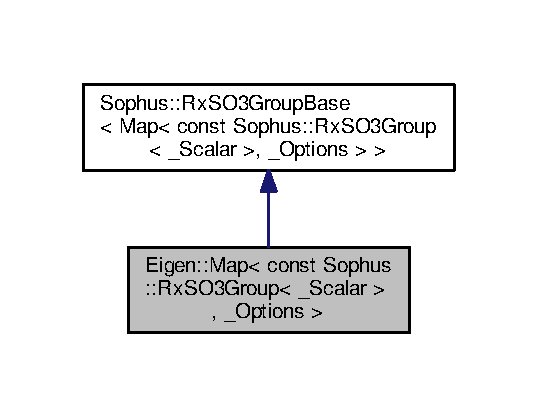
\includegraphics[width=258pt]{class_eigen_1_1_map_3_01const_01_sophus_1_1_rx_s_o3_group_3_01___scalar_01_4_00_01___options_01_4__inherit__graph}
\end{center}
\end{figure}


Collaboration diagram for Eigen\+:\+:Map$<$ const Sophus\+:\+:Rx\+S\+O3\+Group$<$ \+\_\+\+Scalar $>$, \+\_\+\+Options $>$\+:
\nopagebreak
\begin{figure}[H]
\begin{center}
\leavevmode
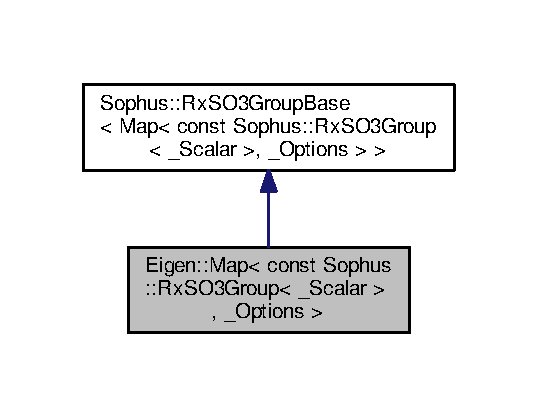
\includegraphics[width=258pt]{class_eigen_1_1_map_3_01const_01_sophus_1_1_rx_s_o3_group_3_01___scalar_01_4_00_01___options_01_4__coll__graph}
\end{center}
\end{figure}
\subsection*{Public Types}
\begin{DoxyCompactItemize}
\item 
typedef internal\+::traits$<$ Map $>$\+::\hyperlink{class_eigen_1_1_map_3_01const_01_sophus_1_1_rx_s_o3_group_3_01___scalar_01_4_00_01___options_01_4_a1d6dec9e4f7cd797ae48d46a7f99daba}{Scalar} \hyperlink{class_eigen_1_1_map_3_01const_01_sophus_1_1_rx_s_o3_group_3_01___scalar_01_4_00_01___options_01_4_a1d6dec9e4f7cd797ae48d46a7f99daba}{Scalar}\hypertarget{class_eigen_1_1_map_3_01const_01_sophus_1_1_rx_s_o3_group_3_01___scalar_01_4_00_01___options_01_4_a1d6dec9e4f7cd797ae48d46a7f99daba}{}\label{class_eigen_1_1_map_3_01const_01_sophus_1_1_rx_s_o3_group_3_01___scalar_01_4_00_01___options_01_4_a1d6dec9e4f7cd797ae48d46a7f99daba}

\begin{DoxyCompactList}\small\item\em scalar type \end{DoxyCompactList}\item 
typedef const internal\+::traits$<$ Map $>$\+::Quaternion\+Type \& \hyperlink{class_eigen_1_1_map_3_01const_01_sophus_1_1_rx_s_o3_group_3_01___scalar_01_4_00_01___options_01_4_a324fba2fcc38f7b982b29894da76b1b2}{Const\+Quaternion\+Reference}\hypertarget{class_eigen_1_1_map_3_01const_01_sophus_1_1_rx_s_o3_group_3_01___scalar_01_4_00_01___options_01_4_a324fba2fcc38f7b982b29894da76b1b2}{}\label{class_eigen_1_1_map_3_01const_01_sophus_1_1_rx_s_o3_group_3_01___scalar_01_4_00_01___options_01_4_a324fba2fcc38f7b982b29894da76b1b2}

\begin{DoxyCompactList}\small\item\em quaternion const reference type \end{DoxyCompactList}\item 
typedef \hyperlink{class_sophus_1_1_rx_s_o3_group_base_a60b2d8cd20692d3d39e5e7c729d95145}{Base\+::\+Transformation} \hyperlink{class_eigen_1_1_map_3_01const_01_sophus_1_1_rx_s_o3_group_3_01___scalar_01_4_00_01___options_01_4_abe8ad8f5cd048eb23577619dd44d146e}{Transformation}\hypertarget{class_eigen_1_1_map_3_01const_01_sophus_1_1_rx_s_o3_group_3_01___scalar_01_4_00_01___options_01_4_abe8ad8f5cd048eb23577619dd44d146e}{}\label{class_eigen_1_1_map_3_01const_01_sophus_1_1_rx_s_o3_group_3_01___scalar_01_4_00_01___options_01_4_abe8ad8f5cd048eb23577619dd44d146e}

\begin{DoxyCompactList}\small\item\em group transfomation type \end{DoxyCompactList}\item 
typedef \hyperlink{class_sophus_1_1_rx_s_o3_group_base_ad2d1b35ab03f6e91a80c2e78f07114a0}{Base\+::\+Point} \hyperlink{class_eigen_1_1_map_3_01const_01_sophus_1_1_rx_s_o3_group_3_01___scalar_01_4_00_01___options_01_4_a9f68fb8029377d4b33f4bafd4cb00159}{Point}\hypertarget{class_eigen_1_1_map_3_01const_01_sophus_1_1_rx_s_o3_group_3_01___scalar_01_4_00_01___options_01_4_a9f68fb8029377d4b33f4bafd4cb00159}{}\label{class_eigen_1_1_map_3_01const_01_sophus_1_1_rx_s_o3_group_3_01___scalar_01_4_00_01___options_01_4_a9f68fb8029377d4b33f4bafd4cb00159}

\begin{DoxyCompactList}\small\item\em point type \end{DoxyCompactList}\item 
typedef \hyperlink{class_sophus_1_1_rx_s_o3_group_base_aa1c4034b0a69496b28f1e81fdc7510c5}{Base\+::\+Tangent} \hyperlink{class_eigen_1_1_map_3_01const_01_sophus_1_1_rx_s_o3_group_3_01___scalar_01_4_00_01___options_01_4_a756f916a830202b1f69efb3765b60ba3}{Tangent}\hypertarget{class_eigen_1_1_map_3_01const_01_sophus_1_1_rx_s_o3_group_3_01___scalar_01_4_00_01___options_01_4_a756f916a830202b1f69efb3765b60ba3}{}\label{class_eigen_1_1_map_3_01const_01_sophus_1_1_rx_s_o3_group_3_01___scalar_01_4_00_01___options_01_4_a756f916a830202b1f69efb3765b60ba3}

\begin{DoxyCompactList}\small\item\em tangent vector type \end{DoxyCompactList}\item 
typedef \hyperlink{class_sophus_1_1_rx_s_o3_group_base_a3f7cc9982043bf0082b7946f566a8179}{Base\+::\+Adjoint} \hyperlink{class_eigen_1_1_map_3_01const_01_sophus_1_1_rx_s_o3_group_3_01___scalar_01_4_00_01___options_01_4_a251b274bca8cbf7d39ceb06714c488d9}{Adjoint}\hypertarget{class_eigen_1_1_map_3_01const_01_sophus_1_1_rx_s_o3_group_3_01___scalar_01_4_00_01___options_01_4_a251b274bca8cbf7d39ceb06714c488d9}{}\label{class_eigen_1_1_map_3_01const_01_sophus_1_1_rx_s_o3_group_3_01___scalar_01_4_00_01___options_01_4_a251b274bca8cbf7d39ceb06714c488d9}

\begin{DoxyCompactList}\small\item\em adjoint transformation type \end{DoxyCompactList}\end{DoxyCompactItemize}
\subsection*{Public Member Functions}
\begin{DoxyCompactItemize}
\item 
E\+I\+G\+E\+N\+\_\+\+S\+T\+R\+O\+N\+G\+\_\+\+I\+N\+L\+I\+NE {\bfseries Map} (const \hyperlink{class_eigen_1_1_map_3_01const_01_sophus_1_1_rx_s_o3_group_3_01___scalar_01_4_00_01___options_01_4_a1d6dec9e4f7cd797ae48d46a7f99daba}{Scalar} $\ast$coeffs)\hypertarget{class_eigen_1_1_map_3_01const_01_sophus_1_1_rx_s_o3_group_3_01___scalar_01_4_00_01___options_01_4_ad97a1ded3dc832e906ce893a08fa2270}{}\label{class_eigen_1_1_map_3_01const_01_sophus_1_1_rx_s_o3_group_3_01___scalar_01_4_00_01___options_01_4_ad97a1ded3dc832e906ce893a08fa2270}

\item 
E\+I\+G\+E\+N\+\_\+\+S\+T\+R\+O\+N\+G\+\_\+\+I\+N\+L\+I\+NE \hyperlink{class_eigen_1_1_map_3_01const_01_sophus_1_1_rx_s_o3_group_3_01___scalar_01_4_00_01___options_01_4_a324fba2fcc38f7b982b29894da76b1b2}{Const\+Quaternion\+Reference} \hyperlink{class_eigen_1_1_map_3_01const_01_sophus_1_1_rx_s_o3_group_3_01___scalar_01_4_00_01___options_01_4_a60393dbd35314cd4838d140fefd69604}{quaternion} () const 
\begin{DoxyCompactList}\small\item\em Accessor of unit quaternion. \end{DoxyCompactList}\end{DoxyCompactItemize}
\subsection*{Static Public Attributes}
\begin{DoxyCompactItemize}
\item 
static const int \hyperlink{class_eigen_1_1_map_3_01const_01_sophus_1_1_rx_s_o3_group_3_01___scalar_01_4_00_01___options_01_4_a18297cfca5b1edf54fa8cc3aef8fe731}{DoF} = Base\+::\+DoF\hypertarget{class_eigen_1_1_map_3_01const_01_sophus_1_1_rx_s_o3_group_3_01___scalar_01_4_00_01___options_01_4_a18297cfca5b1edf54fa8cc3aef8fe731}{}\label{class_eigen_1_1_map_3_01const_01_sophus_1_1_rx_s_o3_group_3_01___scalar_01_4_00_01___options_01_4_a18297cfca5b1edf54fa8cc3aef8fe731}

\begin{DoxyCompactList}\small\item\em degree of freedom of group \end{DoxyCompactList}\item 
static const int \hyperlink{class_eigen_1_1_map_3_01const_01_sophus_1_1_rx_s_o3_group_3_01___scalar_01_4_00_01___options_01_4_afd48c0e838cd85b833f5f0c3586b33d5}{num\+\_\+parameters} = Base\+::num\+\_\+parameters\hypertarget{class_eigen_1_1_map_3_01const_01_sophus_1_1_rx_s_o3_group_3_01___scalar_01_4_00_01___options_01_4_afd48c0e838cd85b833f5f0c3586b33d5}{}\label{class_eigen_1_1_map_3_01const_01_sophus_1_1_rx_s_o3_group_3_01___scalar_01_4_00_01___options_01_4_afd48c0e838cd85b833f5f0c3586b33d5}

\begin{DoxyCompactList}\small\item\em number of internal parameters used \end{DoxyCompactList}\item 
static const int \hyperlink{class_eigen_1_1_map_3_01const_01_sophus_1_1_rx_s_o3_group_3_01___scalar_01_4_00_01___options_01_4_aa20bc32d5308a278b2006974a2776b44}{N} = Base\+::N\hypertarget{class_eigen_1_1_map_3_01const_01_sophus_1_1_rx_s_o3_group_3_01___scalar_01_4_00_01___options_01_4_aa20bc32d5308a278b2006974a2776b44}{}\label{class_eigen_1_1_map_3_01const_01_sophus_1_1_rx_s_o3_group_3_01___scalar_01_4_00_01___options_01_4_aa20bc32d5308a278b2006974a2776b44}

\begin{DoxyCompactList}\small\item\em group transformations are NxN matrices \end{DoxyCompactList}\end{DoxyCompactItemize}
\subsection*{Protected Attributes}
\begin{DoxyCompactItemize}
\item 
const Map$<$ const Quaternion$<$ \hyperlink{class_eigen_1_1_map_3_01const_01_sophus_1_1_rx_s_o3_group_3_01___scalar_01_4_00_01___options_01_4_a1d6dec9e4f7cd797ae48d46a7f99daba}{Scalar} $>$, \+\_\+\+Options $>$ {\bfseries quaternion\+\_\+}\hypertarget{class_eigen_1_1_map_3_01const_01_sophus_1_1_rx_s_o3_group_3_01___scalar_01_4_00_01___options_01_4_aa5eb74879caa618f4c0c2e7d32a24f01}{}\label{class_eigen_1_1_map_3_01const_01_sophus_1_1_rx_s_o3_group_3_01___scalar_01_4_00_01___options_01_4_aa5eb74879caa618f4c0c2e7d32a24f01}

\end{DoxyCompactItemize}
\subsection*{Additional Inherited Members}


\subsection{Detailed Description}
\subsubsection*{template$<$typename \+\_\+\+Scalar, int \+\_\+\+Options$>$\\*
class Eigen\+::\+Map$<$ const Sophus\+::\+Rx\+S\+O3\+Group$<$ \+\_\+\+Scalar $>$, \+\_\+\+Options $>$}

Specialisation of Eigen\+::\+Map for const Rx\+S\+O3\+Group\+Base. 

Allows us to wrap Rx\+S\+O3 Objects around P\+OD array (e.\+g. external c style quaternion) 

Definition at line 786 of file rxso3.\+hpp.



\subsection{Member Function Documentation}
\index{Eigen\+::\+Map$<$ const Sophus\+::\+Rx\+S\+O3\+Group$<$ \+\_\+\+Scalar $>$, \+\_\+\+Options $>$@{Eigen\+::\+Map$<$ const Sophus\+::\+Rx\+S\+O3\+Group$<$ \+\_\+\+Scalar $>$, \+\_\+\+Options $>$}!quaternion@{quaternion}}
\index{quaternion@{quaternion}!Eigen\+::\+Map$<$ const Sophus\+::\+Rx\+S\+O3\+Group$<$ \+\_\+\+Scalar $>$, \+\_\+\+Options $>$@{Eigen\+::\+Map$<$ const Sophus\+::\+Rx\+S\+O3\+Group$<$ \+\_\+\+Scalar $>$, \+\_\+\+Options $>$}}
\subsubsection[{\texorpdfstring{quaternion() const }{quaternion() const }}]{\setlength{\rightskip}{0pt plus 5cm}template$<$typename \+\_\+\+Scalar , int \+\_\+\+Options$>$ E\+I\+G\+E\+N\+\_\+\+S\+T\+R\+O\+N\+G\+\_\+\+I\+N\+L\+I\+NE {\bf Const\+Quaternion\+Reference} Eigen\+::\+Map$<$ const {\bf Sophus\+::\+Rx\+S\+O3\+Group}$<$ \+\_\+\+Scalar $>$, \+\_\+\+Options $>$\+::quaternion (
\begin{DoxyParamCaption}
{}
\end{DoxyParamCaption}
) const\hspace{0.3cm}{\ttfamily [inline]}}\hypertarget{class_eigen_1_1_map_3_01const_01_sophus_1_1_rx_s_o3_group_3_01___scalar_01_4_00_01___options_01_4_a60393dbd35314cd4838d140fefd69604}{}\label{class_eigen_1_1_map_3_01const_01_sophus_1_1_rx_s_o3_group_3_01___scalar_01_4_00_01___options_01_4_a60393dbd35314cd4838d140fefd69604}


Accessor of unit quaternion. 

No direct write access is given to ensure the quaternion stays normalized. 

Definition at line 828 of file rxso3.\+hpp.



The documentation for this class was generated from the following file\+:\begin{DoxyCompactItemize}
\item 
include/\+Sophus/sophus/rxso3.\+hpp\end{DoxyCompactItemize}

\hypertarget{class_eigen_1_1_map_3_01const_01_sophus_1_1_s_e2_group_3_01___scalar_01_4_00_01___options_01_4}{}\section{Eigen\+:\+:Map$<$ const Sophus\+:\+:S\+E2\+Group$<$ \+\_\+\+Scalar $>$, \+\_\+\+Options $>$ Class Template Reference}
\label{class_eigen_1_1_map_3_01const_01_sophus_1_1_s_e2_group_3_01___scalar_01_4_00_01___options_01_4}\index{Eigen\+::\+Map$<$ const Sophus\+::\+S\+E2\+Group$<$ \+\_\+\+Scalar $>$, \+\_\+\+Options $>$@{Eigen\+::\+Map$<$ const Sophus\+::\+S\+E2\+Group$<$ \+\_\+\+Scalar $>$, \+\_\+\+Options $>$}}


Specialisation of Eigen\+::\+Map for const S\+E2\+Group\+Base.  




{\ttfamily \#include $<$se2.\+hpp$>$}



Inheritance diagram for Eigen\+:\+:Map$<$ const Sophus\+:\+:S\+E2\+Group$<$ \+\_\+\+Scalar $>$, \+\_\+\+Options $>$\+:
\nopagebreak
\begin{figure}[H]
\begin{center}
\leavevmode
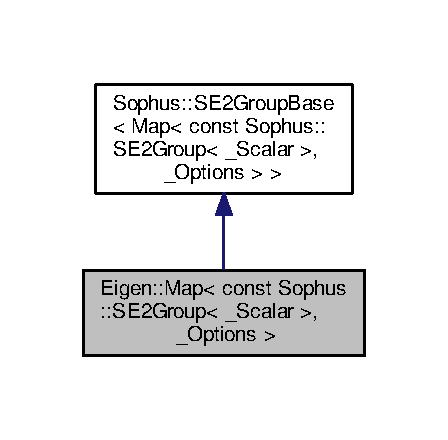
\includegraphics[width=215pt]{class_eigen_1_1_map_3_01const_01_sophus_1_1_s_e2_group_3_01___scalar_01_4_00_01___options_01_4__inherit__graph}
\end{center}
\end{figure}


Collaboration diagram for Eigen\+:\+:Map$<$ const Sophus\+:\+:S\+E2\+Group$<$ \+\_\+\+Scalar $>$, \+\_\+\+Options $>$\+:
\nopagebreak
\begin{figure}[H]
\begin{center}
\leavevmode
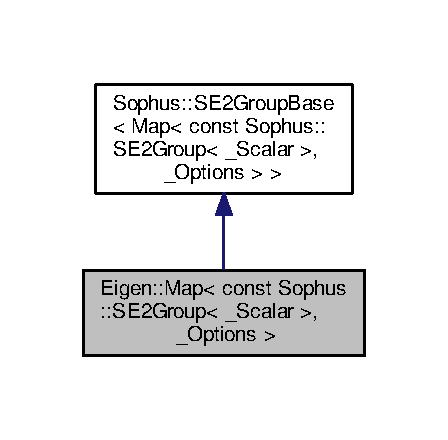
\includegraphics[width=215pt]{class_eigen_1_1_map_3_01const_01_sophus_1_1_s_e2_group_3_01___scalar_01_4_00_01___options_01_4__coll__graph}
\end{center}
\end{figure}
\subsection*{Public Types}
\begin{DoxyCompactItemize}
\item 
typedef internal\+::traits$<$ Map $>$\+::\hyperlink{class_eigen_1_1_map_3_01const_01_sophus_1_1_s_e2_group_3_01___scalar_01_4_00_01___options_01_4_a650e0e4b02a9d2374857c53ff39f5649}{Scalar} \hyperlink{class_eigen_1_1_map_3_01const_01_sophus_1_1_s_e2_group_3_01___scalar_01_4_00_01___options_01_4_a650e0e4b02a9d2374857c53ff39f5649}{Scalar}\hypertarget{class_eigen_1_1_map_3_01const_01_sophus_1_1_s_e2_group_3_01___scalar_01_4_00_01___options_01_4_a650e0e4b02a9d2374857c53ff39f5649}{}\label{class_eigen_1_1_map_3_01const_01_sophus_1_1_s_e2_group_3_01___scalar_01_4_00_01___options_01_4_a650e0e4b02a9d2374857c53ff39f5649}

\begin{DoxyCompactList}\small\item\em scalar type \end{DoxyCompactList}\item 
typedef const internal\+::traits$<$ Map $>$\+::Translation\+Type \& \hyperlink{class_eigen_1_1_map_3_01const_01_sophus_1_1_s_e2_group_3_01___scalar_01_4_00_01___options_01_4_a1f66099d992183637c4ac5bb1792f02d}{Const\+Translation\+Reference}\hypertarget{class_eigen_1_1_map_3_01const_01_sophus_1_1_s_e2_group_3_01___scalar_01_4_00_01___options_01_4_a1f66099d992183637c4ac5bb1792f02d}{}\label{class_eigen_1_1_map_3_01const_01_sophus_1_1_s_e2_group_3_01___scalar_01_4_00_01___options_01_4_a1f66099d992183637c4ac5bb1792f02d}

\begin{DoxyCompactList}\small\item\em translation reference type \end{DoxyCompactList}\item 
typedef const internal\+::traits$<$ Map $>$\+::S\+O2\+Type \& \hyperlink{class_eigen_1_1_map_3_01const_01_sophus_1_1_s_e2_group_3_01___scalar_01_4_00_01___options_01_4_a82e98c7b87974f4673520af28fd36576}{Const\+S\+O2\+Reference}\hypertarget{class_eigen_1_1_map_3_01const_01_sophus_1_1_s_e2_group_3_01___scalar_01_4_00_01___options_01_4_a82e98c7b87974f4673520af28fd36576}{}\label{class_eigen_1_1_map_3_01const_01_sophus_1_1_s_e2_group_3_01___scalar_01_4_00_01___options_01_4_a82e98c7b87974f4673520af28fd36576}

\begin{DoxyCompactList}\small\item\em S\+O2 const reference type. \end{DoxyCompactList}\item 
typedef \hyperlink{class_sophus_1_1_s_e2_group_base_a82fe531d4b64813525d4ebd131da9bcd}{Base\+::\+Transformation} \hyperlink{class_eigen_1_1_map_3_01const_01_sophus_1_1_s_e2_group_3_01___scalar_01_4_00_01___options_01_4_a87ef59de1f0625b721f67841156c50cd}{Transformation}\hypertarget{class_eigen_1_1_map_3_01const_01_sophus_1_1_s_e2_group_3_01___scalar_01_4_00_01___options_01_4_a87ef59de1f0625b721f67841156c50cd}{}\label{class_eigen_1_1_map_3_01const_01_sophus_1_1_s_e2_group_3_01___scalar_01_4_00_01___options_01_4_a87ef59de1f0625b721f67841156c50cd}

\begin{DoxyCompactList}\small\item\em group transfomation type \end{DoxyCompactList}\item 
typedef \hyperlink{class_sophus_1_1_s_e2_group_base_add8b024098bc6fcecdefb42229fa881b}{Base\+::\+Point} \hyperlink{class_eigen_1_1_map_3_01const_01_sophus_1_1_s_e2_group_3_01___scalar_01_4_00_01___options_01_4_a611e19a05a728ff1dc6f4c6840e17f96}{Point}\hypertarget{class_eigen_1_1_map_3_01const_01_sophus_1_1_s_e2_group_3_01___scalar_01_4_00_01___options_01_4_a611e19a05a728ff1dc6f4c6840e17f96}{}\label{class_eigen_1_1_map_3_01const_01_sophus_1_1_s_e2_group_3_01___scalar_01_4_00_01___options_01_4_a611e19a05a728ff1dc6f4c6840e17f96}

\begin{DoxyCompactList}\small\item\em point type \end{DoxyCompactList}\item 
typedef \hyperlink{class_sophus_1_1_s_e2_group_base_a71b41e6cde48514241c7bffcbe34923f}{Base\+::\+Tangent} \hyperlink{class_eigen_1_1_map_3_01const_01_sophus_1_1_s_e2_group_3_01___scalar_01_4_00_01___options_01_4_a22fd2f27e57cac3634e24ca75a0a964d}{Tangent}\hypertarget{class_eigen_1_1_map_3_01const_01_sophus_1_1_s_e2_group_3_01___scalar_01_4_00_01___options_01_4_a22fd2f27e57cac3634e24ca75a0a964d}{}\label{class_eigen_1_1_map_3_01const_01_sophus_1_1_s_e2_group_3_01___scalar_01_4_00_01___options_01_4_a22fd2f27e57cac3634e24ca75a0a964d}

\begin{DoxyCompactList}\small\item\em tangent vector type \end{DoxyCompactList}\item 
typedef \hyperlink{class_sophus_1_1_s_e2_group_base_a6e0785a6f8399456a8bd0b057bae02ee}{Base\+::\+Adjoint} \hyperlink{class_eigen_1_1_map_3_01const_01_sophus_1_1_s_e2_group_3_01___scalar_01_4_00_01___options_01_4_abeebe6c7e688393dc67227e681d788c8}{Adjoint}\hypertarget{class_eigen_1_1_map_3_01const_01_sophus_1_1_s_e2_group_3_01___scalar_01_4_00_01___options_01_4_abeebe6c7e688393dc67227e681d788c8}{}\label{class_eigen_1_1_map_3_01const_01_sophus_1_1_s_e2_group_3_01___scalar_01_4_00_01___options_01_4_abeebe6c7e688393dc67227e681d788c8}

\begin{DoxyCompactList}\small\item\em adjoint transformation type \end{DoxyCompactList}\end{DoxyCompactItemize}
\subsection*{Public Member Functions}
\begin{DoxyCompactItemize}
\item 
E\+I\+G\+E\+N\+\_\+\+S\+T\+R\+O\+N\+G\+\_\+\+I\+N\+L\+I\+NE {\bfseries Map} (const \hyperlink{class_eigen_1_1_map_3_01const_01_sophus_1_1_s_e2_group_3_01___scalar_01_4_00_01___options_01_4_a650e0e4b02a9d2374857c53ff39f5649}{Scalar} $\ast$coeffs)\hypertarget{class_eigen_1_1_map_3_01const_01_sophus_1_1_s_e2_group_3_01___scalar_01_4_00_01___options_01_4_a2f1e39f89bd464ffe5d3cf2a57d94993}{}\label{class_eigen_1_1_map_3_01const_01_sophus_1_1_s_e2_group_3_01___scalar_01_4_00_01___options_01_4_a2f1e39f89bd464ffe5d3cf2a57d94993}

\item 
E\+I\+G\+E\+N\+\_\+\+S\+T\+R\+O\+N\+G\+\_\+\+I\+N\+L\+I\+NE {\bfseries Map} (const \hyperlink{class_eigen_1_1_map_3_01const_01_sophus_1_1_s_e2_group_3_01___scalar_01_4_00_01___options_01_4_a650e0e4b02a9d2374857c53ff39f5649}{Scalar} $\ast$trans\+\_\+coeffs, const \hyperlink{class_eigen_1_1_map_3_01const_01_sophus_1_1_s_e2_group_3_01___scalar_01_4_00_01___options_01_4_a650e0e4b02a9d2374857c53ff39f5649}{Scalar} $\ast$rot\+\_\+coeffs)\hypertarget{class_eigen_1_1_map_3_01const_01_sophus_1_1_s_e2_group_3_01___scalar_01_4_00_01___options_01_4_ab0275ba559b39e37052675338fbfdb93}{}\label{class_eigen_1_1_map_3_01const_01_sophus_1_1_s_e2_group_3_01___scalar_01_4_00_01___options_01_4_ab0275ba559b39e37052675338fbfdb93}

\item 
E\+I\+G\+E\+N\+\_\+\+S\+T\+R\+O\+N\+G\+\_\+\+I\+N\+L\+I\+NE \hyperlink{class_eigen_1_1_map_3_01const_01_sophus_1_1_s_e2_group_3_01___scalar_01_4_00_01___options_01_4_a82e98c7b87974f4673520af28fd36576}{Const\+S\+O2\+Reference} \hyperlink{class_eigen_1_1_map_3_01const_01_sophus_1_1_s_e2_group_3_01___scalar_01_4_00_01___options_01_4_a6244c172ef46455ad6e6c5a8d2817b11}{so2} () const \hypertarget{class_eigen_1_1_map_3_01const_01_sophus_1_1_s_e2_group_3_01___scalar_01_4_00_01___options_01_4_a6244c172ef46455ad6e6c5a8d2817b11}{}\label{class_eigen_1_1_map_3_01const_01_sophus_1_1_s_e2_group_3_01___scalar_01_4_00_01___options_01_4_a6244c172ef46455ad6e6c5a8d2817b11}

\begin{DoxyCompactList}\small\item\em Accessor of S\+O2. \end{DoxyCompactList}\item 
E\+I\+G\+E\+N\+\_\+\+S\+T\+R\+O\+N\+G\+\_\+\+I\+N\+L\+I\+NE \hyperlink{class_eigen_1_1_map_3_01const_01_sophus_1_1_s_e2_group_3_01___scalar_01_4_00_01___options_01_4_a1f66099d992183637c4ac5bb1792f02d}{Const\+Translation\+Reference} \hyperlink{class_eigen_1_1_map_3_01const_01_sophus_1_1_s_e2_group_3_01___scalar_01_4_00_01___options_01_4_a55ae0805a31a76a51d78f9ce33eb299a}{translation} () const \hypertarget{class_eigen_1_1_map_3_01const_01_sophus_1_1_s_e2_group_3_01___scalar_01_4_00_01___options_01_4_a55ae0805a31a76a51d78f9ce33eb299a}{}\label{class_eigen_1_1_map_3_01const_01_sophus_1_1_s_e2_group_3_01___scalar_01_4_00_01___options_01_4_a55ae0805a31a76a51d78f9ce33eb299a}

\begin{DoxyCompactList}\small\item\em Accessor of translation vector. \end{DoxyCompactList}\end{DoxyCompactItemize}
\subsection*{Static Public Attributes}
\begin{DoxyCompactItemize}
\item 
static const int \hyperlink{class_eigen_1_1_map_3_01const_01_sophus_1_1_s_e2_group_3_01___scalar_01_4_00_01___options_01_4_a98b98a8b69f5fc4ea213ced179d66e55}{DoF} = Base\+::\+DoF\hypertarget{class_eigen_1_1_map_3_01const_01_sophus_1_1_s_e2_group_3_01___scalar_01_4_00_01___options_01_4_a98b98a8b69f5fc4ea213ced179d66e55}{}\label{class_eigen_1_1_map_3_01const_01_sophus_1_1_s_e2_group_3_01___scalar_01_4_00_01___options_01_4_a98b98a8b69f5fc4ea213ced179d66e55}

\begin{DoxyCompactList}\small\item\em degree of freedom of group \end{DoxyCompactList}\item 
static const int \hyperlink{class_eigen_1_1_map_3_01const_01_sophus_1_1_s_e2_group_3_01___scalar_01_4_00_01___options_01_4_af73c0d37c33c14364723647c543f5dde}{num\+\_\+parameters} = Base\+::num\+\_\+parameters\hypertarget{class_eigen_1_1_map_3_01const_01_sophus_1_1_s_e2_group_3_01___scalar_01_4_00_01___options_01_4_af73c0d37c33c14364723647c543f5dde}{}\label{class_eigen_1_1_map_3_01const_01_sophus_1_1_s_e2_group_3_01___scalar_01_4_00_01___options_01_4_af73c0d37c33c14364723647c543f5dde}

\begin{DoxyCompactList}\small\item\em number of internal parameters used \end{DoxyCompactList}\item 
static const int \hyperlink{class_eigen_1_1_map_3_01const_01_sophus_1_1_s_e2_group_3_01___scalar_01_4_00_01___options_01_4_a15d00955ee636a4f92c3becade1b2786}{N} = Base\+::N\hypertarget{class_eigen_1_1_map_3_01const_01_sophus_1_1_s_e2_group_3_01___scalar_01_4_00_01___options_01_4_a15d00955ee636a4f92c3becade1b2786}{}\label{class_eigen_1_1_map_3_01const_01_sophus_1_1_s_e2_group_3_01___scalar_01_4_00_01___options_01_4_a15d00955ee636a4f92c3becade1b2786}

\begin{DoxyCompactList}\small\item\em group transformations are NxN matrices \end{DoxyCompactList}\end{DoxyCompactItemize}
\subsection*{Protected Attributes}
\begin{DoxyCompactItemize}
\item 
const Map$<$ const \hyperlink{class_sophus_1_1_s_o2_group}{Sophus\+::\+S\+O2\+Group}$<$ \hyperlink{class_eigen_1_1_map_3_01const_01_sophus_1_1_s_e2_group_3_01___scalar_01_4_00_01___options_01_4_a650e0e4b02a9d2374857c53ff39f5649}{Scalar} $>$, \+\_\+\+Options $>$ {\bfseries so2\+\_\+}\hypertarget{class_eigen_1_1_map_3_01const_01_sophus_1_1_s_e2_group_3_01___scalar_01_4_00_01___options_01_4_a3d635e50c759cabbed1ccb89e0a59b1d}{}\label{class_eigen_1_1_map_3_01const_01_sophus_1_1_s_e2_group_3_01___scalar_01_4_00_01___options_01_4_a3d635e50c759cabbed1ccb89e0a59b1d}

\item 
const Map$<$ const Matrix$<$ \hyperlink{class_eigen_1_1_map_3_01const_01_sophus_1_1_s_e2_group_3_01___scalar_01_4_00_01___options_01_4_a650e0e4b02a9d2374857c53ff39f5649}{Scalar}, 2, 1 $>$, \+\_\+\+Options $>$ {\bfseries translation\+\_\+}\hypertarget{class_eigen_1_1_map_3_01const_01_sophus_1_1_s_e2_group_3_01___scalar_01_4_00_01___options_01_4_ace013fbca399e772d6b6b58d0242bd8b}{}\label{class_eigen_1_1_map_3_01const_01_sophus_1_1_s_e2_group_3_01___scalar_01_4_00_01___options_01_4_ace013fbca399e772d6b6b58d0242bd8b}

\end{DoxyCompactItemize}
\subsection*{Additional Inherited Members}


\subsection{Detailed Description}
\subsubsection*{template$<$typename \+\_\+\+Scalar, int \+\_\+\+Options$>$\\*
class Eigen\+::\+Map$<$ const Sophus\+::\+S\+E2\+Group$<$ \+\_\+\+Scalar $>$, \+\_\+\+Options $>$}

Specialisation of Eigen\+::\+Map for const S\+E2\+Group\+Base. 

Allows us to wrap S\+E2 Objects around P\+OD array (e.\+g. external c style complex) 

Definition at line 839 of file se2.\+hpp.



The documentation for this class was generated from the following file\+:\begin{DoxyCompactItemize}
\item 
include/\+Sophus/sophus/se2.\+hpp\end{DoxyCompactItemize}

\hypertarget{class_eigen_1_1_map_3_01const_01_sophus_1_1_s_e3_group_3_01___scalar_01_4_00_01___options_01_4}{}\section{Eigen\+:\+:Map$<$ const Sophus\+:\+:S\+E3\+Group$<$ \+\_\+\+Scalar $>$, \+\_\+\+Options $>$ Class Template Reference}
\label{class_eigen_1_1_map_3_01const_01_sophus_1_1_s_e3_group_3_01___scalar_01_4_00_01___options_01_4}\index{Eigen\+::\+Map$<$ const Sophus\+::\+S\+E3\+Group$<$ \+\_\+\+Scalar $>$, \+\_\+\+Options $>$@{Eigen\+::\+Map$<$ const Sophus\+::\+S\+E3\+Group$<$ \+\_\+\+Scalar $>$, \+\_\+\+Options $>$}}


Specialisation of Eigen\+::\+Map for const S\+E3\+Group\+Base.  




{\ttfamily \#include $<$se3.\+hpp$>$}



Inheritance diagram for Eigen\+:\+:Map$<$ const Sophus\+:\+:S\+E3\+Group$<$ \+\_\+\+Scalar $>$, \+\_\+\+Options $>$\+:
\nopagebreak
\begin{figure}[H]
\begin{center}
\leavevmode
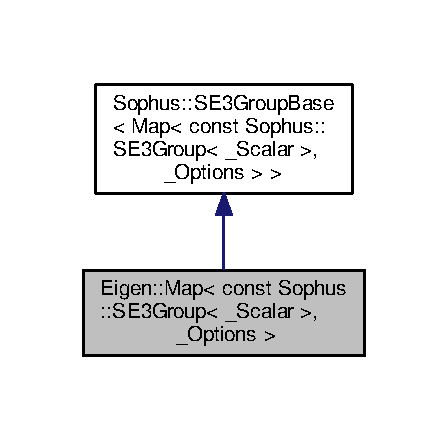
\includegraphics[width=215pt]{class_eigen_1_1_map_3_01const_01_sophus_1_1_s_e3_group_3_01___scalar_01_4_00_01___options_01_4__inherit__graph}
\end{center}
\end{figure}


Collaboration diagram for Eigen\+:\+:Map$<$ const Sophus\+:\+:S\+E3\+Group$<$ \+\_\+\+Scalar $>$, \+\_\+\+Options $>$\+:
\nopagebreak
\begin{figure}[H]
\begin{center}
\leavevmode
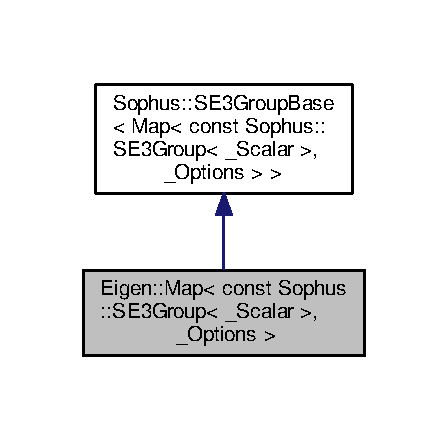
\includegraphics[width=215pt]{class_eigen_1_1_map_3_01const_01_sophus_1_1_s_e3_group_3_01___scalar_01_4_00_01___options_01_4__coll__graph}
\end{center}
\end{figure}
\subsection*{Public Types}
\begin{DoxyCompactItemize}
\item 
typedef internal\+::traits$<$ Map $>$\+::\hyperlink{class_eigen_1_1_map_3_01const_01_sophus_1_1_s_e3_group_3_01___scalar_01_4_00_01___options_01_4_a24b7cfd38fbe43026ced1fab3cc19584}{Scalar} \hyperlink{class_eigen_1_1_map_3_01const_01_sophus_1_1_s_e3_group_3_01___scalar_01_4_00_01___options_01_4_a24b7cfd38fbe43026ced1fab3cc19584}{Scalar}\hypertarget{class_eigen_1_1_map_3_01const_01_sophus_1_1_s_e3_group_3_01___scalar_01_4_00_01___options_01_4_a24b7cfd38fbe43026ced1fab3cc19584}{}\label{class_eigen_1_1_map_3_01const_01_sophus_1_1_s_e3_group_3_01___scalar_01_4_00_01___options_01_4_a24b7cfd38fbe43026ced1fab3cc19584}

\begin{DoxyCompactList}\small\item\em scalar type \end{DoxyCompactList}\item 
typedef const internal\+::traits$<$ Map $>$\+::Translation\+Type \& \hyperlink{class_eigen_1_1_map_3_01const_01_sophus_1_1_s_e3_group_3_01___scalar_01_4_00_01___options_01_4_a30dee589eb6520b39aaeabefb7685a98}{Const\+Translation\+Reference}\hypertarget{class_eigen_1_1_map_3_01const_01_sophus_1_1_s_e3_group_3_01___scalar_01_4_00_01___options_01_4_a30dee589eb6520b39aaeabefb7685a98}{}\label{class_eigen_1_1_map_3_01const_01_sophus_1_1_s_e3_group_3_01___scalar_01_4_00_01___options_01_4_a30dee589eb6520b39aaeabefb7685a98}

\begin{DoxyCompactList}\small\item\em translation const reference type \end{DoxyCompactList}\item 
typedef const internal\+::traits$<$ Map $>$\+::S\+O3\+Type \& \hyperlink{class_eigen_1_1_map_3_01const_01_sophus_1_1_s_e3_group_3_01___scalar_01_4_00_01___options_01_4_adfa2d5c638577360f8069013cc5059aa}{Const\+S\+O3\+Reference}\hypertarget{class_eigen_1_1_map_3_01const_01_sophus_1_1_s_e3_group_3_01___scalar_01_4_00_01___options_01_4_adfa2d5c638577360f8069013cc5059aa}{}\label{class_eigen_1_1_map_3_01const_01_sophus_1_1_s_e3_group_3_01___scalar_01_4_00_01___options_01_4_adfa2d5c638577360f8069013cc5059aa}

\begin{DoxyCompactList}\small\item\em S\+O3 const reference type. \end{DoxyCompactList}\item 
typedef \hyperlink{class_sophus_1_1_s_e3_group_base_a426ebd53f324a4fd6d36c28028f967f1}{Base\+::\+Transformation} \hyperlink{class_eigen_1_1_map_3_01const_01_sophus_1_1_s_e3_group_3_01___scalar_01_4_00_01___options_01_4_aee2efbe24d6a0891ff96d41c37c8d1e0}{Transformation}\hypertarget{class_eigen_1_1_map_3_01const_01_sophus_1_1_s_e3_group_3_01___scalar_01_4_00_01___options_01_4_aee2efbe24d6a0891ff96d41c37c8d1e0}{}\label{class_eigen_1_1_map_3_01const_01_sophus_1_1_s_e3_group_3_01___scalar_01_4_00_01___options_01_4_aee2efbe24d6a0891ff96d41c37c8d1e0}

\begin{DoxyCompactList}\small\item\em group transfomation type \end{DoxyCompactList}\item 
typedef \hyperlink{class_sophus_1_1_s_e3_group_base_aca2cf20e857567b74fb399c7ee76c744}{Base\+::\+Point} \hyperlink{class_eigen_1_1_map_3_01const_01_sophus_1_1_s_e3_group_3_01___scalar_01_4_00_01___options_01_4_a20a09e0d881c88d5f44c3139fe26b518}{Point}\hypertarget{class_eigen_1_1_map_3_01const_01_sophus_1_1_s_e3_group_3_01___scalar_01_4_00_01___options_01_4_a20a09e0d881c88d5f44c3139fe26b518}{}\label{class_eigen_1_1_map_3_01const_01_sophus_1_1_s_e3_group_3_01___scalar_01_4_00_01___options_01_4_a20a09e0d881c88d5f44c3139fe26b518}

\begin{DoxyCompactList}\small\item\em point type \end{DoxyCompactList}\item 
typedef \hyperlink{class_sophus_1_1_s_e3_group_base_a45f63b562f0614853cef2c04c4cd5f2b}{Base\+::\+Tangent} \hyperlink{class_eigen_1_1_map_3_01const_01_sophus_1_1_s_e3_group_3_01___scalar_01_4_00_01___options_01_4_a86a2a734aa756360254c0a48bcfccb81}{Tangent}\hypertarget{class_eigen_1_1_map_3_01const_01_sophus_1_1_s_e3_group_3_01___scalar_01_4_00_01___options_01_4_a86a2a734aa756360254c0a48bcfccb81}{}\label{class_eigen_1_1_map_3_01const_01_sophus_1_1_s_e3_group_3_01___scalar_01_4_00_01___options_01_4_a86a2a734aa756360254c0a48bcfccb81}

\begin{DoxyCompactList}\small\item\em tangent vector type \end{DoxyCompactList}\item 
typedef \hyperlink{class_sophus_1_1_s_e3_group_base_ac2e0179cb3e9490604c417d8e59a92d3}{Base\+::\+Adjoint} \hyperlink{class_eigen_1_1_map_3_01const_01_sophus_1_1_s_e3_group_3_01___scalar_01_4_00_01___options_01_4_ab4e354d68c235a9e4869cd4f59670981}{Adjoint}\hypertarget{class_eigen_1_1_map_3_01const_01_sophus_1_1_s_e3_group_3_01___scalar_01_4_00_01___options_01_4_ab4e354d68c235a9e4869cd4f59670981}{}\label{class_eigen_1_1_map_3_01const_01_sophus_1_1_s_e3_group_3_01___scalar_01_4_00_01___options_01_4_ab4e354d68c235a9e4869cd4f59670981}

\begin{DoxyCompactList}\small\item\em adjoint transformation type \end{DoxyCompactList}\end{DoxyCompactItemize}
\subsection*{Public Member Functions}
\begin{DoxyCompactItemize}
\item 
E\+I\+G\+E\+N\+\_\+\+S\+T\+R\+O\+N\+G\+\_\+\+I\+N\+L\+I\+NE {\bfseries Map} (const \hyperlink{class_eigen_1_1_map_3_01const_01_sophus_1_1_s_e3_group_3_01___scalar_01_4_00_01___options_01_4_a24b7cfd38fbe43026ced1fab3cc19584}{Scalar} $\ast$coeffs)\hypertarget{class_eigen_1_1_map_3_01const_01_sophus_1_1_s_e3_group_3_01___scalar_01_4_00_01___options_01_4_a5b85ade38803ccbcb43db362c799f1ac}{}\label{class_eigen_1_1_map_3_01const_01_sophus_1_1_s_e3_group_3_01___scalar_01_4_00_01___options_01_4_a5b85ade38803ccbcb43db362c799f1ac}

\item 
E\+I\+G\+E\+N\+\_\+\+S\+T\+R\+O\+N\+G\+\_\+\+I\+N\+L\+I\+NE {\bfseries Map} (const \hyperlink{class_eigen_1_1_map_3_01const_01_sophus_1_1_s_e3_group_3_01___scalar_01_4_00_01___options_01_4_a24b7cfd38fbe43026ced1fab3cc19584}{Scalar} $\ast$trans\+\_\+coeffs, const \hyperlink{class_eigen_1_1_map_3_01const_01_sophus_1_1_s_e3_group_3_01___scalar_01_4_00_01___options_01_4_a24b7cfd38fbe43026ced1fab3cc19584}{Scalar} $\ast$rot\+\_\+coeffs)\hypertarget{class_eigen_1_1_map_3_01const_01_sophus_1_1_s_e3_group_3_01___scalar_01_4_00_01___options_01_4_abacab3585fcd9458fec27e6b8f35c8ee}{}\label{class_eigen_1_1_map_3_01const_01_sophus_1_1_s_e3_group_3_01___scalar_01_4_00_01___options_01_4_abacab3585fcd9458fec27e6b8f35c8ee}

\item 
E\+I\+G\+E\+N\+\_\+\+S\+T\+R\+O\+N\+G\+\_\+\+I\+N\+L\+I\+NE \hyperlink{class_eigen_1_1_map_3_01const_01_sophus_1_1_s_e3_group_3_01___scalar_01_4_00_01___options_01_4_adfa2d5c638577360f8069013cc5059aa}{Const\+S\+O3\+Reference} \hyperlink{class_eigen_1_1_map_3_01const_01_sophus_1_1_s_e3_group_3_01___scalar_01_4_00_01___options_01_4_a921b87abc465b3242ed2481e58e695a0}{so3} () const \hypertarget{class_eigen_1_1_map_3_01const_01_sophus_1_1_s_e3_group_3_01___scalar_01_4_00_01___options_01_4_a921b87abc465b3242ed2481e58e695a0}{}\label{class_eigen_1_1_map_3_01const_01_sophus_1_1_s_e3_group_3_01___scalar_01_4_00_01___options_01_4_a921b87abc465b3242ed2481e58e695a0}

\begin{DoxyCompactList}\small\item\em Accessor of S\+O3. \end{DoxyCompactList}\item 
E\+I\+G\+E\+N\+\_\+\+S\+T\+R\+O\+N\+G\+\_\+\+I\+N\+L\+I\+NE \hyperlink{class_eigen_1_1_map_3_01const_01_sophus_1_1_s_e3_group_3_01___scalar_01_4_00_01___options_01_4_a30dee589eb6520b39aaeabefb7685a98}{Const\+Translation\+Reference} \hyperlink{class_eigen_1_1_map_3_01const_01_sophus_1_1_s_e3_group_3_01___scalar_01_4_00_01___options_01_4_afb907b6cd2c8119952bb7f58a7f7b189}{translation} () const \hypertarget{class_eigen_1_1_map_3_01const_01_sophus_1_1_s_e3_group_3_01___scalar_01_4_00_01___options_01_4_afb907b6cd2c8119952bb7f58a7f7b189}{}\label{class_eigen_1_1_map_3_01const_01_sophus_1_1_s_e3_group_3_01___scalar_01_4_00_01___options_01_4_afb907b6cd2c8119952bb7f58a7f7b189}

\begin{DoxyCompactList}\small\item\em Accessor of translation vector. \end{DoxyCompactList}\end{DoxyCompactItemize}
\subsection*{Static Public Attributes}
\begin{DoxyCompactItemize}
\item 
static const int \hyperlink{class_eigen_1_1_map_3_01const_01_sophus_1_1_s_e3_group_3_01___scalar_01_4_00_01___options_01_4_a2044d22d524b14e440498d1c7a1af8ad}{DoF} = Base\+::\+DoF\hypertarget{class_eigen_1_1_map_3_01const_01_sophus_1_1_s_e3_group_3_01___scalar_01_4_00_01___options_01_4_a2044d22d524b14e440498d1c7a1af8ad}{}\label{class_eigen_1_1_map_3_01const_01_sophus_1_1_s_e3_group_3_01___scalar_01_4_00_01___options_01_4_a2044d22d524b14e440498d1c7a1af8ad}

\begin{DoxyCompactList}\small\item\em degree of freedom of group \end{DoxyCompactList}\item 
static const int \hyperlink{class_eigen_1_1_map_3_01const_01_sophus_1_1_s_e3_group_3_01___scalar_01_4_00_01___options_01_4_aec41bcc240ff5eb4f2c61428d6b52b36}{num\+\_\+parameters} = Base\+::num\+\_\+parameters\hypertarget{class_eigen_1_1_map_3_01const_01_sophus_1_1_s_e3_group_3_01___scalar_01_4_00_01___options_01_4_aec41bcc240ff5eb4f2c61428d6b52b36}{}\label{class_eigen_1_1_map_3_01const_01_sophus_1_1_s_e3_group_3_01___scalar_01_4_00_01___options_01_4_aec41bcc240ff5eb4f2c61428d6b52b36}

\begin{DoxyCompactList}\small\item\em number of internal parameters used \end{DoxyCompactList}\item 
static const int \hyperlink{class_eigen_1_1_map_3_01const_01_sophus_1_1_s_e3_group_3_01___scalar_01_4_00_01___options_01_4_a6e19d03e06d07e12dbcb0a790af72718}{N} = Base\+::N\hypertarget{class_eigen_1_1_map_3_01const_01_sophus_1_1_s_e3_group_3_01___scalar_01_4_00_01___options_01_4_a6e19d03e06d07e12dbcb0a790af72718}{}\label{class_eigen_1_1_map_3_01const_01_sophus_1_1_s_e3_group_3_01___scalar_01_4_00_01___options_01_4_a6e19d03e06d07e12dbcb0a790af72718}

\begin{DoxyCompactList}\small\item\em group transformations are NxN matrices \end{DoxyCompactList}\end{DoxyCompactItemize}
\subsection*{Protected Attributes}
\begin{DoxyCompactItemize}
\item 
const Map$<$ const \hyperlink{class_sophus_1_1_s_o3_group}{Sophus\+::\+S\+O3\+Group}$<$ \hyperlink{class_eigen_1_1_map_3_01const_01_sophus_1_1_s_e3_group_3_01___scalar_01_4_00_01___options_01_4_a24b7cfd38fbe43026ced1fab3cc19584}{Scalar} $>$, \+\_\+\+Options $>$ {\bfseries so3\+\_\+}\hypertarget{class_eigen_1_1_map_3_01const_01_sophus_1_1_s_e3_group_3_01___scalar_01_4_00_01___options_01_4_afb6011ed06d79247c95c5af8cdce23ce}{}\label{class_eigen_1_1_map_3_01const_01_sophus_1_1_s_e3_group_3_01___scalar_01_4_00_01___options_01_4_afb6011ed06d79247c95c5af8cdce23ce}

\item 
const Map$<$ const Matrix$<$ \hyperlink{class_eigen_1_1_map_3_01const_01_sophus_1_1_s_e3_group_3_01___scalar_01_4_00_01___options_01_4_a24b7cfd38fbe43026ced1fab3cc19584}{Scalar}, 3, 1 $>$, \+\_\+\+Options $>$ {\bfseries translation\+\_\+}\hypertarget{class_eigen_1_1_map_3_01const_01_sophus_1_1_s_e3_group_3_01___scalar_01_4_00_01___options_01_4_a01fbfadf1de3692aeef4fa4f7a41fb56}{}\label{class_eigen_1_1_map_3_01const_01_sophus_1_1_s_e3_group_3_01___scalar_01_4_00_01___options_01_4_a01fbfadf1de3692aeef4fa4f7a41fb56}

\end{DoxyCompactItemize}
\subsection*{Additional Inherited Members}


\subsection{Detailed Description}
\subsubsection*{template$<$typename \+\_\+\+Scalar, int \+\_\+\+Options$>$\\*
class Eigen\+::\+Map$<$ const Sophus\+::\+S\+E3\+Group$<$ \+\_\+\+Scalar $>$, \+\_\+\+Options $>$}

Specialisation of Eigen\+::\+Map for const S\+E3\+Group\+Base. 

Allows us to wrap S\+E3 Objects around P\+OD array (e.\+g. external c style quaternion) 

Definition at line 878 of file se3.\+hpp.



The documentation for this class was generated from the following file\+:\begin{DoxyCompactItemize}
\item 
include/\+Sophus/sophus/se3.\+hpp\end{DoxyCompactItemize}

\hypertarget{class_eigen_1_1_map_3_01const_01_sophus_1_1_sim3_group_3_01___scalar_01_4_00_01___options_01_4}{}\section{Eigen\+:\+:Map$<$ const Sophus\+:\+:Sim3\+Group$<$ \+\_\+\+Scalar $>$, \+\_\+\+Options $>$ Class Template Reference}
\label{class_eigen_1_1_map_3_01const_01_sophus_1_1_sim3_group_3_01___scalar_01_4_00_01___options_01_4}\index{Eigen\+::\+Map$<$ const Sophus\+::\+Sim3\+Group$<$ \+\_\+\+Scalar $>$, \+\_\+\+Options $>$@{Eigen\+::\+Map$<$ const Sophus\+::\+Sim3\+Group$<$ \+\_\+\+Scalar $>$, \+\_\+\+Options $>$}}


Specialisation of Eigen\+::\+Map for const Sim3\+Group\+Base.  




{\ttfamily \#include $<$sim3.\+hpp$>$}



Inheritance diagram for Eigen\+:\+:Map$<$ const Sophus\+:\+:Sim3\+Group$<$ \+\_\+\+Scalar $>$, \+\_\+\+Options $>$\+:
\nopagebreak
\begin{figure}[H]
\begin{center}
\leavevmode
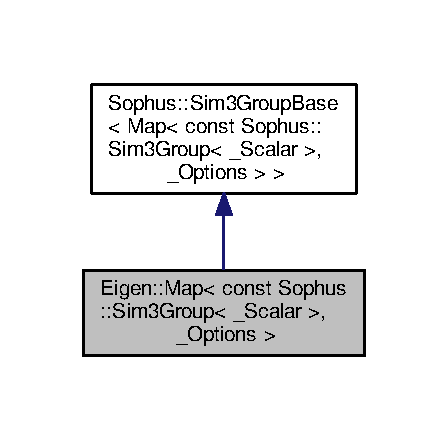
\includegraphics[width=215pt]{class_eigen_1_1_map_3_01const_01_sophus_1_1_sim3_group_3_01___scalar_01_4_00_01___options_01_4__inherit__graph}
\end{center}
\end{figure}


Collaboration diagram for Eigen\+:\+:Map$<$ const Sophus\+:\+:Sim3\+Group$<$ \+\_\+\+Scalar $>$, \+\_\+\+Options $>$\+:
\nopagebreak
\begin{figure}[H]
\begin{center}
\leavevmode
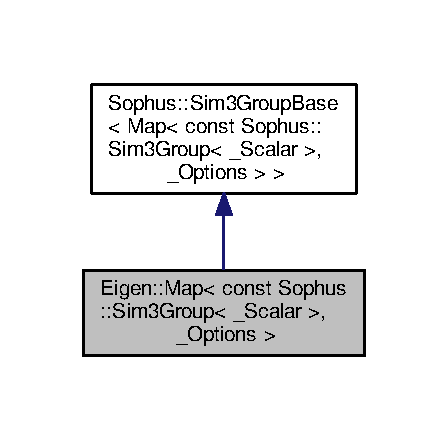
\includegraphics[width=215pt]{class_eigen_1_1_map_3_01const_01_sophus_1_1_sim3_group_3_01___scalar_01_4_00_01___options_01_4__coll__graph}
\end{center}
\end{figure}
\subsection*{Public Types}
\begin{DoxyCompactItemize}
\item 
typedef internal\+::traits$<$ Map $>$\+::\hyperlink{class_eigen_1_1_map_3_01const_01_sophus_1_1_sim3_group_3_01___scalar_01_4_00_01___options_01_4_af8769c2970043ae3c4a88ced33b421a9}{Scalar} \hyperlink{class_eigen_1_1_map_3_01const_01_sophus_1_1_sim3_group_3_01___scalar_01_4_00_01___options_01_4_af8769c2970043ae3c4a88ced33b421a9}{Scalar}\hypertarget{class_eigen_1_1_map_3_01const_01_sophus_1_1_sim3_group_3_01___scalar_01_4_00_01___options_01_4_af8769c2970043ae3c4a88ced33b421a9}{}\label{class_eigen_1_1_map_3_01const_01_sophus_1_1_sim3_group_3_01___scalar_01_4_00_01___options_01_4_af8769c2970043ae3c4a88ced33b421a9}

\begin{DoxyCompactList}\small\item\em scalar type \end{DoxyCompactList}\item 
typedef const internal\+::traits$<$ Map $>$\+::Translation\+Type \& \hyperlink{class_eigen_1_1_map_3_01const_01_sophus_1_1_sim3_group_3_01___scalar_01_4_00_01___options_01_4_a1b5c44cd51659f195655a0a20e506289}{Const\+Translation\+Reference}\hypertarget{class_eigen_1_1_map_3_01const_01_sophus_1_1_sim3_group_3_01___scalar_01_4_00_01___options_01_4_a1b5c44cd51659f195655a0a20e506289}{}\label{class_eigen_1_1_map_3_01const_01_sophus_1_1_sim3_group_3_01___scalar_01_4_00_01___options_01_4_a1b5c44cd51659f195655a0a20e506289}

\begin{DoxyCompactList}\small\item\em translation type \end{DoxyCompactList}\item 
typedef const internal\+::traits$<$ Map $>$\+::Rx\+S\+O3\+Type \& \hyperlink{class_eigen_1_1_map_3_01const_01_sophus_1_1_sim3_group_3_01___scalar_01_4_00_01___options_01_4_a486ddf84534c6214b62fa62540883248}{Const\+Rx\+S\+O3\+Reference}\hypertarget{class_eigen_1_1_map_3_01const_01_sophus_1_1_sim3_group_3_01___scalar_01_4_00_01___options_01_4_a486ddf84534c6214b62fa62540883248}{}\label{class_eigen_1_1_map_3_01const_01_sophus_1_1_sim3_group_3_01___scalar_01_4_00_01___options_01_4_a486ddf84534c6214b62fa62540883248}

\begin{DoxyCompactList}\small\item\em Rx\+S\+O3 const reference type. \end{DoxyCompactList}\item 
typedef \hyperlink{class_sophus_1_1_sim3_group_base_a93c8c564e3386709dc4cb2fc6d451dd8}{Base\+::\+Transformation} \hyperlink{class_eigen_1_1_map_3_01const_01_sophus_1_1_sim3_group_3_01___scalar_01_4_00_01___options_01_4_af0731324b4f87bdc1319578bb5ca66d8}{Transformation}\hypertarget{class_eigen_1_1_map_3_01const_01_sophus_1_1_sim3_group_3_01___scalar_01_4_00_01___options_01_4_af0731324b4f87bdc1319578bb5ca66d8}{}\label{class_eigen_1_1_map_3_01const_01_sophus_1_1_sim3_group_3_01___scalar_01_4_00_01___options_01_4_af0731324b4f87bdc1319578bb5ca66d8}

\begin{DoxyCompactList}\small\item\em group transfomation type \end{DoxyCompactList}\item 
typedef \hyperlink{class_sophus_1_1_sim3_group_base_a4b50c6b94e402746e50076305781dc9d}{Base\+::\+Point} \hyperlink{class_eigen_1_1_map_3_01const_01_sophus_1_1_sim3_group_3_01___scalar_01_4_00_01___options_01_4_aa65a3a9194d830594c4270e802ed7081}{Point}\hypertarget{class_eigen_1_1_map_3_01const_01_sophus_1_1_sim3_group_3_01___scalar_01_4_00_01___options_01_4_aa65a3a9194d830594c4270e802ed7081}{}\label{class_eigen_1_1_map_3_01const_01_sophus_1_1_sim3_group_3_01___scalar_01_4_00_01___options_01_4_aa65a3a9194d830594c4270e802ed7081}

\begin{DoxyCompactList}\small\item\em point type \end{DoxyCompactList}\item 
typedef \hyperlink{class_sophus_1_1_sim3_group_base_a0f61582b6d8fa46ecbb40d70c87b632c}{Base\+::\+Tangent} \hyperlink{class_eigen_1_1_map_3_01const_01_sophus_1_1_sim3_group_3_01___scalar_01_4_00_01___options_01_4_ad62dd21ea3767ee340cea881297a9be9}{Tangent}\hypertarget{class_eigen_1_1_map_3_01const_01_sophus_1_1_sim3_group_3_01___scalar_01_4_00_01___options_01_4_ad62dd21ea3767ee340cea881297a9be9}{}\label{class_eigen_1_1_map_3_01const_01_sophus_1_1_sim3_group_3_01___scalar_01_4_00_01___options_01_4_ad62dd21ea3767ee340cea881297a9be9}

\begin{DoxyCompactList}\small\item\em tangent vector type \end{DoxyCompactList}\item 
typedef \hyperlink{class_sophus_1_1_sim3_group_base_a7aa93f325ac7b811db77652f488e8f03}{Base\+::\+Adjoint} \hyperlink{class_eigen_1_1_map_3_01const_01_sophus_1_1_sim3_group_3_01___scalar_01_4_00_01___options_01_4_a85f83127420b7335dbac6a9d35cd9b72}{Adjoint}\hypertarget{class_eigen_1_1_map_3_01const_01_sophus_1_1_sim3_group_3_01___scalar_01_4_00_01___options_01_4_a85f83127420b7335dbac6a9d35cd9b72}{}\label{class_eigen_1_1_map_3_01const_01_sophus_1_1_sim3_group_3_01___scalar_01_4_00_01___options_01_4_a85f83127420b7335dbac6a9d35cd9b72}

\begin{DoxyCompactList}\small\item\em adjoint transformation type \end{DoxyCompactList}\end{DoxyCompactItemize}
\subsection*{Public Member Functions}
\begin{DoxyCompactItemize}
\item 
E\+I\+G\+E\+N\+\_\+\+S\+T\+R\+O\+N\+G\+\_\+\+I\+N\+L\+I\+NE {\bfseries Map} (const \hyperlink{class_eigen_1_1_map_3_01const_01_sophus_1_1_sim3_group_3_01___scalar_01_4_00_01___options_01_4_af8769c2970043ae3c4a88ced33b421a9}{Scalar} $\ast$coeffs)\hypertarget{class_eigen_1_1_map_3_01const_01_sophus_1_1_sim3_group_3_01___scalar_01_4_00_01___options_01_4_af08dcceecb9adf3b91ac39652bc9392c}{}\label{class_eigen_1_1_map_3_01const_01_sophus_1_1_sim3_group_3_01___scalar_01_4_00_01___options_01_4_af08dcceecb9adf3b91ac39652bc9392c}

\item 
E\+I\+G\+E\+N\+\_\+\+S\+T\+R\+O\+N\+G\+\_\+\+I\+N\+L\+I\+NE {\bfseries Map} (const \hyperlink{class_eigen_1_1_map_3_01const_01_sophus_1_1_sim3_group_3_01___scalar_01_4_00_01___options_01_4_af8769c2970043ae3c4a88ced33b421a9}{Scalar} $\ast$trans\+\_\+coeffs, const \hyperlink{class_eigen_1_1_map_3_01const_01_sophus_1_1_sim3_group_3_01___scalar_01_4_00_01___options_01_4_af8769c2970043ae3c4a88ced33b421a9}{Scalar} $\ast$rot\+\_\+coeffs)\hypertarget{class_eigen_1_1_map_3_01const_01_sophus_1_1_sim3_group_3_01___scalar_01_4_00_01___options_01_4_ac57395062f5344a9c75ab856eae26dc2}{}\label{class_eigen_1_1_map_3_01const_01_sophus_1_1_sim3_group_3_01___scalar_01_4_00_01___options_01_4_ac57395062f5344a9c75ab856eae26dc2}

\item 
E\+I\+G\+E\+N\+\_\+\+S\+T\+R\+O\+N\+G\+\_\+\+I\+N\+L\+I\+NE \hyperlink{class_eigen_1_1_map_3_01const_01_sophus_1_1_sim3_group_3_01___scalar_01_4_00_01___options_01_4_a486ddf84534c6214b62fa62540883248}{Const\+Rx\+S\+O3\+Reference} \hyperlink{class_eigen_1_1_map_3_01const_01_sophus_1_1_sim3_group_3_01___scalar_01_4_00_01___options_01_4_a7c2afd35051a3406d96d01b59f169775}{rxso3} () const \hypertarget{class_eigen_1_1_map_3_01const_01_sophus_1_1_sim3_group_3_01___scalar_01_4_00_01___options_01_4_a7c2afd35051a3406d96d01b59f169775}{}\label{class_eigen_1_1_map_3_01const_01_sophus_1_1_sim3_group_3_01___scalar_01_4_00_01___options_01_4_a7c2afd35051a3406d96d01b59f169775}

\begin{DoxyCompactList}\small\item\em Accessor of Rx\+S\+O3. \end{DoxyCompactList}\item 
E\+I\+G\+E\+N\+\_\+\+S\+T\+R\+O\+N\+G\+\_\+\+I\+N\+L\+I\+NE \hyperlink{class_eigen_1_1_map_3_01const_01_sophus_1_1_sim3_group_3_01___scalar_01_4_00_01___options_01_4_a1b5c44cd51659f195655a0a20e506289}{Const\+Translation\+Reference} \hyperlink{class_eigen_1_1_map_3_01const_01_sophus_1_1_sim3_group_3_01___scalar_01_4_00_01___options_01_4_ae765cb6532155da714a0580912c3285b}{translation} () const \hypertarget{class_eigen_1_1_map_3_01const_01_sophus_1_1_sim3_group_3_01___scalar_01_4_00_01___options_01_4_ae765cb6532155da714a0580912c3285b}{}\label{class_eigen_1_1_map_3_01const_01_sophus_1_1_sim3_group_3_01___scalar_01_4_00_01___options_01_4_ae765cb6532155da714a0580912c3285b}

\begin{DoxyCompactList}\small\item\em Accessor of translation vector. \end{DoxyCompactList}\end{DoxyCompactItemize}
\subsection*{Static Public Attributes}
\begin{DoxyCompactItemize}
\item 
static const int \hyperlink{class_eigen_1_1_map_3_01const_01_sophus_1_1_sim3_group_3_01___scalar_01_4_00_01___options_01_4_af4ea6f060b5c831d8a14cd39e63f7afa}{DoF} = Base\+::\+DoF\hypertarget{class_eigen_1_1_map_3_01const_01_sophus_1_1_sim3_group_3_01___scalar_01_4_00_01___options_01_4_af4ea6f060b5c831d8a14cd39e63f7afa}{}\label{class_eigen_1_1_map_3_01const_01_sophus_1_1_sim3_group_3_01___scalar_01_4_00_01___options_01_4_af4ea6f060b5c831d8a14cd39e63f7afa}

\begin{DoxyCompactList}\small\item\em degree of freedom of group \end{DoxyCompactList}\item 
static const int \hyperlink{class_eigen_1_1_map_3_01const_01_sophus_1_1_sim3_group_3_01___scalar_01_4_00_01___options_01_4_a9d593284d70a3cfc600947428226c764}{num\+\_\+parameters} = Base\+::num\+\_\+parameters\hypertarget{class_eigen_1_1_map_3_01const_01_sophus_1_1_sim3_group_3_01___scalar_01_4_00_01___options_01_4_a9d593284d70a3cfc600947428226c764}{}\label{class_eigen_1_1_map_3_01const_01_sophus_1_1_sim3_group_3_01___scalar_01_4_00_01___options_01_4_a9d593284d70a3cfc600947428226c764}

\begin{DoxyCompactList}\small\item\em number of internal parameters used \end{DoxyCompactList}\item 
static const int \hyperlink{class_eigen_1_1_map_3_01const_01_sophus_1_1_sim3_group_3_01___scalar_01_4_00_01___options_01_4_a19f718d241c90ff4639378f178f4d78e}{N} = Base\+::N\hypertarget{class_eigen_1_1_map_3_01const_01_sophus_1_1_sim3_group_3_01___scalar_01_4_00_01___options_01_4_a19f718d241c90ff4639378f178f4d78e}{}\label{class_eigen_1_1_map_3_01const_01_sophus_1_1_sim3_group_3_01___scalar_01_4_00_01___options_01_4_a19f718d241c90ff4639378f178f4d78e}

\begin{DoxyCompactList}\small\item\em group transformations are NxN matrices \end{DoxyCompactList}\end{DoxyCompactItemize}
\subsection*{Protected Attributes}
\begin{DoxyCompactItemize}
\item 
const Map$<$ const \hyperlink{class_sophus_1_1_rx_s_o3_group}{Sophus\+::\+Rx\+S\+O3\+Group}$<$ \hyperlink{class_eigen_1_1_map_3_01const_01_sophus_1_1_sim3_group_3_01___scalar_01_4_00_01___options_01_4_af8769c2970043ae3c4a88ced33b421a9}{Scalar} $>$, \+\_\+\+Options $>$ {\bfseries rxso3\+\_\+}\hypertarget{class_eigen_1_1_map_3_01const_01_sophus_1_1_sim3_group_3_01___scalar_01_4_00_01___options_01_4_a3e94c69dc33346a9a192a0eb61bae25b}{}\label{class_eigen_1_1_map_3_01const_01_sophus_1_1_sim3_group_3_01___scalar_01_4_00_01___options_01_4_a3e94c69dc33346a9a192a0eb61bae25b}

\item 
const Map$<$ const Matrix$<$ \hyperlink{class_eigen_1_1_map_3_01const_01_sophus_1_1_sim3_group_3_01___scalar_01_4_00_01___options_01_4_af8769c2970043ae3c4a88ced33b421a9}{Scalar}, 3, 1 $>$, \+\_\+\+Options $>$ {\bfseries translation\+\_\+}\hypertarget{class_eigen_1_1_map_3_01const_01_sophus_1_1_sim3_group_3_01___scalar_01_4_00_01___options_01_4_afb007fc2f029429b11758fc8b4ae078a}{}\label{class_eigen_1_1_map_3_01const_01_sophus_1_1_sim3_group_3_01___scalar_01_4_00_01___options_01_4_afb007fc2f029429b11758fc8b4ae078a}

\end{DoxyCompactItemize}
\subsection*{Additional Inherited Members}


\subsection{Detailed Description}
\subsubsection*{template$<$typename \+\_\+\+Scalar, int \+\_\+\+Options$>$\\*
class Eigen\+::\+Map$<$ const Sophus\+::\+Sim3\+Group$<$ \+\_\+\+Scalar $>$, \+\_\+\+Options $>$}

Specialisation of Eigen\+::\+Map for const Sim3\+Group\+Base. 

Allows us to wrap Sim3 Objects around P\+OD array (e.\+g. external c style quaternion) 

Definition at line 907 of file sim3.\+hpp.



The documentation for this class was generated from the following file\+:\begin{DoxyCompactItemize}
\item 
include/\+Sophus/sophus/sim3.\+hpp\end{DoxyCompactItemize}

\hypertarget{class_eigen_1_1_map_3_01const_01_sophus_1_1_s_o2_group_3_01___scalar_01_4_00_01___options_01_4}{}\section{Eigen\+:\+:Map$<$ const Sophus\+:\+:S\+O2\+Group$<$ \+\_\+\+Scalar $>$, \+\_\+\+Options $>$ Class Template Reference}
\label{class_eigen_1_1_map_3_01const_01_sophus_1_1_s_o2_group_3_01___scalar_01_4_00_01___options_01_4}\index{Eigen\+::\+Map$<$ const Sophus\+::\+S\+O2\+Group$<$ \+\_\+\+Scalar $>$, \+\_\+\+Options $>$@{Eigen\+::\+Map$<$ const Sophus\+::\+S\+O2\+Group$<$ \+\_\+\+Scalar $>$, \+\_\+\+Options $>$}}


Specialisation of Eigen\+::\+Map for const S\+O2\+Group\+Base.  




{\ttfamily \#include $<$so2.\+hpp$>$}



Inheritance diagram for Eigen\+:\+:Map$<$ const Sophus\+:\+:S\+O2\+Group$<$ \+\_\+\+Scalar $>$, \+\_\+\+Options $>$\+:
\nopagebreak
\begin{figure}[H]
\begin{center}
\leavevmode
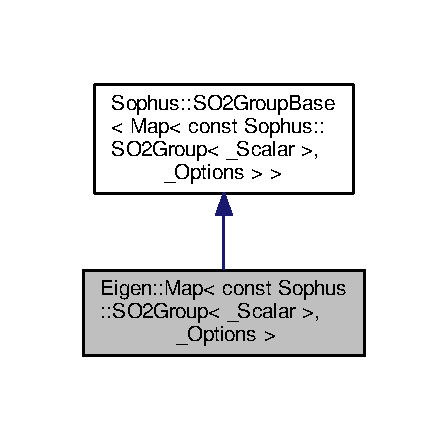
\includegraphics[width=215pt]{class_eigen_1_1_map_3_01const_01_sophus_1_1_s_o2_group_3_01___scalar_01_4_00_01___options_01_4__inherit__graph}
\end{center}
\end{figure}


Collaboration diagram for Eigen\+:\+:Map$<$ const Sophus\+:\+:S\+O2\+Group$<$ \+\_\+\+Scalar $>$, \+\_\+\+Options $>$\+:
\nopagebreak
\begin{figure}[H]
\begin{center}
\leavevmode
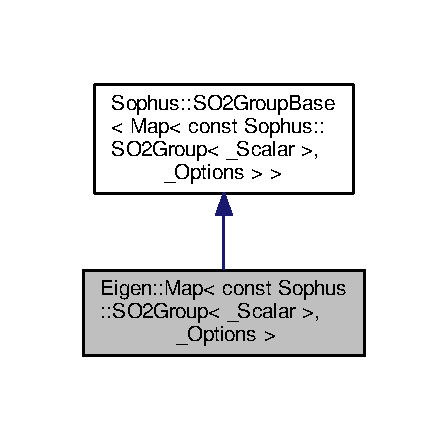
\includegraphics[width=215pt]{class_eigen_1_1_map_3_01const_01_sophus_1_1_s_o2_group_3_01___scalar_01_4_00_01___options_01_4__coll__graph}
\end{center}
\end{figure}
\subsection*{Public Types}
\begin{DoxyCompactItemize}
\item 
typedef internal\+::traits$<$ Map $>$\+::\hyperlink{class_eigen_1_1_map_3_01const_01_sophus_1_1_s_o2_group_3_01___scalar_01_4_00_01___options_01_4_a437464266d5d506a72bca93371ba33f1}{Scalar} \hyperlink{class_eigen_1_1_map_3_01const_01_sophus_1_1_s_o2_group_3_01___scalar_01_4_00_01___options_01_4_a437464266d5d506a72bca93371ba33f1}{Scalar}\hypertarget{class_eigen_1_1_map_3_01const_01_sophus_1_1_s_o2_group_3_01___scalar_01_4_00_01___options_01_4_a437464266d5d506a72bca93371ba33f1}{}\label{class_eigen_1_1_map_3_01const_01_sophus_1_1_s_o2_group_3_01___scalar_01_4_00_01___options_01_4_a437464266d5d506a72bca93371ba33f1}

\begin{DoxyCompactList}\small\item\em scalar type \end{DoxyCompactList}\item 
typedef const internal\+::traits$<$ Map $>$\+::Complex\+Type \& \hyperlink{class_eigen_1_1_map_3_01const_01_sophus_1_1_s_o2_group_3_01___scalar_01_4_00_01___options_01_4_ae8150799b694d2530765a9f8be6a3429}{Const\+Complex\+Reference}\hypertarget{class_eigen_1_1_map_3_01const_01_sophus_1_1_s_o2_group_3_01___scalar_01_4_00_01___options_01_4_ae8150799b694d2530765a9f8be6a3429}{}\label{class_eigen_1_1_map_3_01const_01_sophus_1_1_s_o2_group_3_01___scalar_01_4_00_01___options_01_4_ae8150799b694d2530765a9f8be6a3429}

\begin{DoxyCompactList}\small\item\em complex number const reference type \end{DoxyCompactList}\item 
typedef \hyperlink{class_sophus_1_1_s_o2_group_base_a8981dccaf65802191e989815046b6a82}{Base\+::\+Transformation} \hyperlink{class_eigen_1_1_map_3_01const_01_sophus_1_1_s_o2_group_3_01___scalar_01_4_00_01___options_01_4_a009de720e40e09f2f3e48893f6c7365b}{Transformation}\hypertarget{class_eigen_1_1_map_3_01const_01_sophus_1_1_s_o2_group_3_01___scalar_01_4_00_01___options_01_4_a009de720e40e09f2f3e48893f6c7365b}{}\label{class_eigen_1_1_map_3_01const_01_sophus_1_1_s_o2_group_3_01___scalar_01_4_00_01___options_01_4_a009de720e40e09f2f3e48893f6c7365b}

\begin{DoxyCompactList}\small\item\em group transfomation type \end{DoxyCompactList}\item 
typedef \hyperlink{class_sophus_1_1_s_o2_group_base_acdbb4a45d5f3d826b6bf8462c92c7f54}{Base\+::\+Point} \hyperlink{class_eigen_1_1_map_3_01const_01_sophus_1_1_s_o2_group_3_01___scalar_01_4_00_01___options_01_4_a700eec5bd71bd63cbcd708592dfed726}{Point}\hypertarget{class_eigen_1_1_map_3_01const_01_sophus_1_1_s_o2_group_3_01___scalar_01_4_00_01___options_01_4_a700eec5bd71bd63cbcd708592dfed726}{}\label{class_eigen_1_1_map_3_01const_01_sophus_1_1_s_o2_group_3_01___scalar_01_4_00_01___options_01_4_a700eec5bd71bd63cbcd708592dfed726}

\begin{DoxyCompactList}\small\item\em point type \end{DoxyCompactList}\item 
typedef \hyperlink{class_sophus_1_1_s_o2_group_base_a3701d07bf2791675518a0ceb33ce653b}{Base\+::\+Tangent} \hyperlink{class_eigen_1_1_map_3_01const_01_sophus_1_1_s_o2_group_3_01___scalar_01_4_00_01___options_01_4_a8ec98e2333ee46d7b481aa1046062f46}{Tangent}\hypertarget{class_eigen_1_1_map_3_01const_01_sophus_1_1_s_o2_group_3_01___scalar_01_4_00_01___options_01_4_a8ec98e2333ee46d7b481aa1046062f46}{}\label{class_eigen_1_1_map_3_01const_01_sophus_1_1_s_o2_group_3_01___scalar_01_4_00_01___options_01_4_a8ec98e2333ee46d7b481aa1046062f46}

\begin{DoxyCompactList}\small\item\em tangent vector type \end{DoxyCompactList}\item 
typedef \hyperlink{class_sophus_1_1_s_o2_group_base_a02b4843e52df827cf466eacd288697fa}{Base\+::\+Adjoint} \hyperlink{class_eigen_1_1_map_3_01const_01_sophus_1_1_s_o2_group_3_01___scalar_01_4_00_01___options_01_4_a5e9526d4904397780e06f7d155e08d9c}{Adjoint}\hypertarget{class_eigen_1_1_map_3_01const_01_sophus_1_1_s_o2_group_3_01___scalar_01_4_00_01___options_01_4_a5e9526d4904397780e06f7d155e08d9c}{}\label{class_eigen_1_1_map_3_01const_01_sophus_1_1_s_o2_group_3_01___scalar_01_4_00_01___options_01_4_a5e9526d4904397780e06f7d155e08d9c}

\begin{DoxyCompactList}\small\item\em adjoint transformation type \end{DoxyCompactList}\end{DoxyCompactItemize}
\subsection*{Public Member Functions}
\begin{DoxyCompactItemize}
\item 
E\+I\+G\+E\+N\+\_\+\+S\+T\+R\+O\+N\+G\+\_\+\+I\+N\+L\+I\+NE {\bfseries Map} (const \hyperlink{class_eigen_1_1_map_3_01const_01_sophus_1_1_s_o2_group_3_01___scalar_01_4_00_01___options_01_4_a437464266d5d506a72bca93371ba33f1}{Scalar} $\ast$coeffs)\hypertarget{class_eigen_1_1_map_3_01const_01_sophus_1_1_s_o2_group_3_01___scalar_01_4_00_01___options_01_4_aa42e4d99217223b3ac603c0bc2e45ca1}{}\label{class_eigen_1_1_map_3_01const_01_sophus_1_1_s_o2_group_3_01___scalar_01_4_00_01___options_01_4_aa42e4d99217223b3ac603c0bc2e45ca1}

\item 
E\+I\+G\+E\+N\+\_\+\+S\+T\+R\+O\+N\+G\+\_\+\+I\+N\+L\+I\+NE \hyperlink{class_eigen_1_1_map_3_01const_01_sophus_1_1_s_o2_group_3_01___scalar_01_4_00_01___options_01_4_ae8150799b694d2530765a9f8be6a3429}{Const\+Complex\+Reference} \hyperlink{class_eigen_1_1_map_3_01const_01_sophus_1_1_s_o2_group_3_01___scalar_01_4_00_01___options_01_4_a7ba2acb9c4e8dc4df2f7eaf6ec07e5c0}{unit\+\_\+complex} () const 
\begin{DoxyCompactList}\small\item\em Accessor of unit complex number. \end{DoxyCompactList}\end{DoxyCompactItemize}
\subsection*{Static Public Attributes}
\begin{DoxyCompactItemize}
\item 
static const int \hyperlink{class_eigen_1_1_map_3_01const_01_sophus_1_1_s_o2_group_3_01___scalar_01_4_00_01___options_01_4_ad7931bdb93522d05b5570356f7d8e9a2}{DoF} = Base\+::\+DoF\hypertarget{class_eigen_1_1_map_3_01const_01_sophus_1_1_s_o2_group_3_01___scalar_01_4_00_01___options_01_4_ad7931bdb93522d05b5570356f7d8e9a2}{}\label{class_eigen_1_1_map_3_01const_01_sophus_1_1_s_o2_group_3_01___scalar_01_4_00_01___options_01_4_ad7931bdb93522d05b5570356f7d8e9a2}

\begin{DoxyCompactList}\small\item\em degree of freedom of group \end{DoxyCompactList}\item 
static const int \hyperlink{class_eigen_1_1_map_3_01const_01_sophus_1_1_s_o2_group_3_01___scalar_01_4_00_01___options_01_4_a6fbe2bf93dc0e0f23c3d43ee90bd5857}{num\+\_\+parameters} = Base\+::num\+\_\+parameters\hypertarget{class_eigen_1_1_map_3_01const_01_sophus_1_1_s_o2_group_3_01___scalar_01_4_00_01___options_01_4_a6fbe2bf93dc0e0f23c3d43ee90bd5857}{}\label{class_eigen_1_1_map_3_01const_01_sophus_1_1_s_o2_group_3_01___scalar_01_4_00_01___options_01_4_a6fbe2bf93dc0e0f23c3d43ee90bd5857}

\begin{DoxyCompactList}\small\item\em number of internal parameters used \end{DoxyCompactList}\item 
static const int \hyperlink{class_eigen_1_1_map_3_01const_01_sophus_1_1_s_o2_group_3_01___scalar_01_4_00_01___options_01_4_ae4b28f5a9ab60eac2b58fd99e2b1d72e}{N} = Base\+::N\hypertarget{class_eigen_1_1_map_3_01const_01_sophus_1_1_s_o2_group_3_01___scalar_01_4_00_01___options_01_4_ae4b28f5a9ab60eac2b58fd99e2b1d72e}{}\label{class_eigen_1_1_map_3_01const_01_sophus_1_1_s_o2_group_3_01___scalar_01_4_00_01___options_01_4_ae4b28f5a9ab60eac2b58fd99e2b1d72e}

\begin{DoxyCompactList}\small\item\em group transformations are NxN matrices \end{DoxyCompactList}\end{DoxyCompactItemize}
\subsection*{Protected Attributes}
\begin{DoxyCompactItemize}
\item 
const Map$<$ const Matrix$<$ \hyperlink{class_eigen_1_1_map_3_01const_01_sophus_1_1_s_o2_group_3_01___scalar_01_4_00_01___options_01_4_a437464266d5d506a72bca93371ba33f1}{Scalar}, 2, 1 $>$, \+\_\+\+Options $>$ {\bfseries unit\+\_\+complex\+\_\+}\hypertarget{class_eigen_1_1_map_3_01const_01_sophus_1_1_s_o2_group_3_01___scalar_01_4_00_01___options_01_4_a0b3c442abbf51b6271fe44655c41fc1c}{}\label{class_eigen_1_1_map_3_01const_01_sophus_1_1_s_o2_group_3_01___scalar_01_4_00_01___options_01_4_a0b3c442abbf51b6271fe44655c41fc1c}

\end{DoxyCompactItemize}
\subsection*{Additional Inherited Members}


\subsection{Detailed Description}
\subsubsection*{template$<$typename \+\_\+\+Scalar, int \+\_\+\+Options$>$\\*
class Eigen\+::\+Map$<$ const Sophus\+::\+S\+O2\+Group$<$ \+\_\+\+Scalar $>$, \+\_\+\+Options $>$}

Specialisation of Eigen\+::\+Map for const S\+O2\+Group\+Base. 

Allows us to wrap S\+O2 Objects around P\+OD array (e.\+g. external c style complex number) 

Definition at line 646 of file so2.\+hpp.



\subsection{Member Function Documentation}
\index{Eigen\+::\+Map$<$ const Sophus\+::\+S\+O2\+Group$<$ \+\_\+\+Scalar $>$, \+\_\+\+Options $>$@{Eigen\+::\+Map$<$ const Sophus\+::\+S\+O2\+Group$<$ \+\_\+\+Scalar $>$, \+\_\+\+Options $>$}!unit\+\_\+complex@{unit\+\_\+complex}}
\index{unit\+\_\+complex@{unit\+\_\+complex}!Eigen\+::\+Map$<$ const Sophus\+::\+S\+O2\+Group$<$ \+\_\+\+Scalar $>$, \+\_\+\+Options $>$@{Eigen\+::\+Map$<$ const Sophus\+::\+S\+O2\+Group$<$ \+\_\+\+Scalar $>$, \+\_\+\+Options $>$}}
\subsubsection[{\texorpdfstring{unit\+\_\+complex() const }{unit_complex() const }}]{\setlength{\rightskip}{0pt plus 5cm}template$<$typename \+\_\+\+Scalar , int \+\_\+\+Options$>$ E\+I\+G\+E\+N\+\_\+\+S\+T\+R\+O\+N\+G\+\_\+\+I\+N\+L\+I\+NE {\bf Const\+Complex\+Reference} Eigen\+::\+Map$<$ const {\bf Sophus\+::\+S\+O2\+Group}$<$ \+\_\+\+Scalar $>$, \+\_\+\+Options $>$\+::unit\+\_\+complex (
\begin{DoxyParamCaption}
{}
\end{DoxyParamCaption}
) const\hspace{0.3cm}{\ttfamily [inline]}}\hypertarget{class_eigen_1_1_map_3_01const_01_sophus_1_1_s_o2_group_3_01___scalar_01_4_00_01___options_01_4_a7ba2acb9c4e8dc4df2f7eaf6ec07e5c0}{}\label{class_eigen_1_1_map_3_01const_01_sophus_1_1_s_o2_group_3_01___scalar_01_4_00_01___options_01_4_a7ba2acb9c4e8dc4df2f7eaf6ec07e5c0}


Accessor of unit complex number. 

No direct write access is given to ensure the complex number stays normalized. 

Definition at line 690 of file so2.\+hpp.



The documentation for this class was generated from the following file\+:\begin{DoxyCompactItemize}
\item 
include/\+Sophus/sophus/so2.\+hpp\end{DoxyCompactItemize}

\hypertarget{class_eigen_1_1_map_3_01const_01_sophus_1_1_s_o3_group_3_01___scalar_01_4_00_01___options_01_4}{}\section{Eigen\+:\+:Map$<$ const Sophus\+:\+:S\+O3\+Group$<$ \+\_\+\+Scalar $>$, \+\_\+\+Options $>$ Class Template Reference}
\label{class_eigen_1_1_map_3_01const_01_sophus_1_1_s_o3_group_3_01___scalar_01_4_00_01___options_01_4}\index{Eigen\+::\+Map$<$ const Sophus\+::\+S\+O3\+Group$<$ \+\_\+\+Scalar $>$, \+\_\+\+Options $>$@{Eigen\+::\+Map$<$ const Sophus\+::\+S\+O3\+Group$<$ \+\_\+\+Scalar $>$, \+\_\+\+Options $>$}}


Specialisation of Eigen\+::\+Map for const S\+O3\+Group\+Base.  




{\ttfamily \#include $<$so3.\+hpp$>$}



Inheritance diagram for Eigen\+:\+:Map$<$ const Sophus\+:\+:S\+O3\+Group$<$ \+\_\+\+Scalar $>$, \+\_\+\+Options $>$\+:
\nopagebreak
\begin{figure}[H]
\begin{center}
\leavevmode
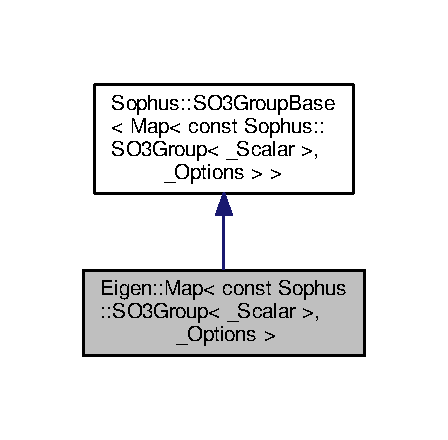
\includegraphics[width=215pt]{class_eigen_1_1_map_3_01const_01_sophus_1_1_s_o3_group_3_01___scalar_01_4_00_01___options_01_4__inherit__graph}
\end{center}
\end{figure}


Collaboration diagram for Eigen\+:\+:Map$<$ const Sophus\+:\+:S\+O3\+Group$<$ \+\_\+\+Scalar $>$, \+\_\+\+Options $>$\+:
\nopagebreak
\begin{figure}[H]
\begin{center}
\leavevmode
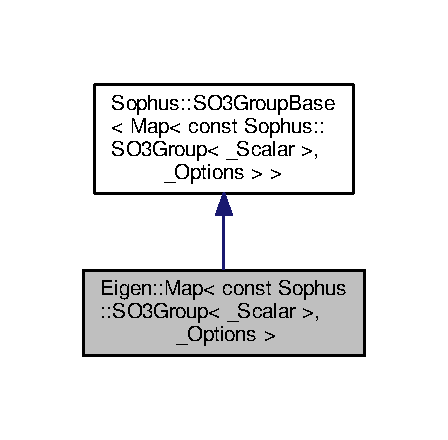
\includegraphics[width=215pt]{class_eigen_1_1_map_3_01const_01_sophus_1_1_s_o3_group_3_01___scalar_01_4_00_01___options_01_4__coll__graph}
\end{center}
\end{figure}
\subsection*{Public Types}
\begin{DoxyCompactItemize}
\item 
typedef internal\+::traits$<$ Map $>$\+::\hyperlink{class_eigen_1_1_map_3_01const_01_sophus_1_1_s_o3_group_3_01___scalar_01_4_00_01___options_01_4_ab140bd002784cc47ef5472ddc8932d9d}{Scalar} \hyperlink{class_eigen_1_1_map_3_01const_01_sophus_1_1_s_o3_group_3_01___scalar_01_4_00_01___options_01_4_ab140bd002784cc47ef5472ddc8932d9d}{Scalar}\hypertarget{class_eigen_1_1_map_3_01const_01_sophus_1_1_s_o3_group_3_01___scalar_01_4_00_01___options_01_4_ab140bd002784cc47ef5472ddc8932d9d}{}\label{class_eigen_1_1_map_3_01const_01_sophus_1_1_s_o3_group_3_01___scalar_01_4_00_01___options_01_4_ab140bd002784cc47ef5472ddc8932d9d}

\begin{DoxyCompactList}\small\item\em scalar type \end{DoxyCompactList}\item 
typedef const internal\+::traits$<$ Map $>$\+::Quaternion\+Type \& \hyperlink{class_eigen_1_1_map_3_01const_01_sophus_1_1_s_o3_group_3_01___scalar_01_4_00_01___options_01_4_af1bc918543cb6466e63a8e6ba82b5d20}{Const\+Quaternion\+Reference}\hypertarget{class_eigen_1_1_map_3_01const_01_sophus_1_1_s_o3_group_3_01___scalar_01_4_00_01___options_01_4_af1bc918543cb6466e63a8e6ba82b5d20}{}\label{class_eigen_1_1_map_3_01const_01_sophus_1_1_s_o3_group_3_01___scalar_01_4_00_01___options_01_4_af1bc918543cb6466e63a8e6ba82b5d20}

\begin{DoxyCompactList}\small\item\em quaternion const reference type \end{DoxyCompactList}\item 
typedef \hyperlink{class_sophus_1_1_s_o3_group_base_aa20fc57bf1b355a6616f5c4b785f1fc5}{Base\+::\+Transformation} \hyperlink{class_eigen_1_1_map_3_01const_01_sophus_1_1_s_o3_group_3_01___scalar_01_4_00_01___options_01_4_a0d788906471a760d74c8323bdcee0e41}{Transformation}\hypertarget{class_eigen_1_1_map_3_01const_01_sophus_1_1_s_o3_group_3_01___scalar_01_4_00_01___options_01_4_a0d788906471a760d74c8323bdcee0e41}{}\label{class_eigen_1_1_map_3_01const_01_sophus_1_1_s_o3_group_3_01___scalar_01_4_00_01___options_01_4_a0d788906471a760d74c8323bdcee0e41}

\begin{DoxyCompactList}\small\item\em group transfomation type \end{DoxyCompactList}\item 
typedef \hyperlink{class_sophus_1_1_s_o3_group_base_a1cfbc3b3a28e1f70b3e1845716db0a1b}{Base\+::\+Point} \hyperlink{class_eigen_1_1_map_3_01const_01_sophus_1_1_s_o3_group_3_01___scalar_01_4_00_01___options_01_4_a4e9ae6a91bf1a0de1e0744c178e91dfb}{Point}\hypertarget{class_eigen_1_1_map_3_01const_01_sophus_1_1_s_o3_group_3_01___scalar_01_4_00_01___options_01_4_a4e9ae6a91bf1a0de1e0744c178e91dfb}{}\label{class_eigen_1_1_map_3_01const_01_sophus_1_1_s_o3_group_3_01___scalar_01_4_00_01___options_01_4_a4e9ae6a91bf1a0de1e0744c178e91dfb}

\begin{DoxyCompactList}\small\item\em point type \end{DoxyCompactList}\item 
typedef \hyperlink{class_sophus_1_1_s_o3_group_base_a11150229b6a471ae96cde974ece5ec7c}{Base\+::\+Tangent} \hyperlink{class_eigen_1_1_map_3_01const_01_sophus_1_1_s_o3_group_3_01___scalar_01_4_00_01___options_01_4_a0821c862738406ea58baeeb7b4dbb1dc}{Tangent}\hypertarget{class_eigen_1_1_map_3_01const_01_sophus_1_1_s_o3_group_3_01___scalar_01_4_00_01___options_01_4_a0821c862738406ea58baeeb7b4dbb1dc}{}\label{class_eigen_1_1_map_3_01const_01_sophus_1_1_s_o3_group_3_01___scalar_01_4_00_01___options_01_4_a0821c862738406ea58baeeb7b4dbb1dc}

\begin{DoxyCompactList}\small\item\em tangent vector type \end{DoxyCompactList}\item 
typedef \hyperlink{class_sophus_1_1_s_o3_group_base_a51c46f75563c21fbd223b4a444923306}{Base\+::\+Adjoint} \hyperlink{class_eigen_1_1_map_3_01const_01_sophus_1_1_s_o3_group_3_01___scalar_01_4_00_01___options_01_4_a926b5e5a3b504d28a12a418a9878e3a8}{Adjoint}\hypertarget{class_eigen_1_1_map_3_01const_01_sophus_1_1_s_o3_group_3_01___scalar_01_4_00_01___options_01_4_a926b5e5a3b504d28a12a418a9878e3a8}{}\label{class_eigen_1_1_map_3_01const_01_sophus_1_1_s_o3_group_3_01___scalar_01_4_00_01___options_01_4_a926b5e5a3b504d28a12a418a9878e3a8}

\begin{DoxyCompactList}\small\item\em adjoint transformation type \end{DoxyCompactList}\end{DoxyCompactItemize}
\subsection*{Public Member Functions}
\begin{DoxyCompactItemize}
\item 
E\+I\+G\+E\+N\+\_\+\+S\+T\+R\+O\+N\+G\+\_\+\+I\+N\+L\+I\+NE {\bfseries Map} (const \hyperlink{class_eigen_1_1_map_3_01const_01_sophus_1_1_s_o3_group_3_01___scalar_01_4_00_01___options_01_4_ab140bd002784cc47ef5472ddc8932d9d}{Scalar} $\ast$coeffs)\hypertarget{class_eigen_1_1_map_3_01const_01_sophus_1_1_s_o3_group_3_01___scalar_01_4_00_01___options_01_4_abf676f1c2ceed3d55429a323a3870eb2}{}\label{class_eigen_1_1_map_3_01const_01_sophus_1_1_s_o3_group_3_01___scalar_01_4_00_01___options_01_4_abf676f1c2ceed3d55429a323a3870eb2}

\item 
E\+I\+G\+E\+N\+\_\+\+S\+T\+R\+O\+N\+G\+\_\+\+I\+N\+L\+I\+NE const \hyperlink{class_eigen_1_1_map_3_01const_01_sophus_1_1_s_o3_group_3_01___scalar_01_4_00_01___options_01_4_af1bc918543cb6466e63a8e6ba82b5d20}{Const\+Quaternion\+Reference} \hyperlink{class_eigen_1_1_map_3_01const_01_sophus_1_1_s_o3_group_3_01___scalar_01_4_00_01___options_01_4_aad2d9300025120be8f92b75cd800d6f6}{unit\+\_\+quaternion} () const 
\begin{DoxyCompactList}\small\item\em Accessor of unit quaternion. \end{DoxyCompactList}\end{DoxyCompactItemize}
\subsection*{Static Public Attributes}
\begin{DoxyCompactItemize}
\item 
static const int \hyperlink{class_eigen_1_1_map_3_01const_01_sophus_1_1_s_o3_group_3_01___scalar_01_4_00_01___options_01_4_a9709869f77f5a10e5f2d7e178feac52b}{DoF} = Base\+::\+DoF\hypertarget{class_eigen_1_1_map_3_01const_01_sophus_1_1_s_o3_group_3_01___scalar_01_4_00_01___options_01_4_a9709869f77f5a10e5f2d7e178feac52b}{}\label{class_eigen_1_1_map_3_01const_01_sophus_1_1_s_o3_group_3_01___scalar_01_4_00_01___options_01_4_a9709869f77f5a10e5f2d7e178feac52b}

\begin{DoxyCompactList}\small\item\em degree of freedom of group \end{DoxyCompactList}\item 
static const int \hyperlink{class_eigen_1_1_map_3_01const_01_sophus_1_1_s_o3_group_3_01___scalar_01_4_00_01___options_01_4_ad3dd5d64fcfa02f2dd7255d6c4f17236}{num\+\_\+parameters} = Base\+::num\+\_\+parameters\hypertarget{class_eigen_1_1_map_3_01const_01_sophus_1_1_s_o3_group_3_01___scalar_01_4_00_01___options_01_4_ad3dd5d64fcfa02f2dd7255d6c4f17236}{}\label{class_eigen_1_1_map_3_01const_01_sophus_1_1_s_o3_group_3_01___scalar_01_4_00_01___options_01_4_ad3dd5d64fcfa02f2dd7255d6c4f17236}

\begin{DoxyCompactList}\small\item\em number of internal parameters used \end{DoxyCompactList}\item 
static const int \hyperlink{class_eigen_1_1_map_3_01const_01_sophus_1_1_s_o3_group_3_01___scalar_01_4_00_01___options_01_4_a1327da79c13c6ce5b97b20f74825e546}{N} = Base\+::N\hypertarget{class_eigen_1_1_map_3_01const_01_sophus_1_1_s_o3_group_3_01___scalar_01_4_00_01___options_01_4_a1327da79c13c6ce5b97b20f74825e546}{}\label{class_eigen_1_1_map_3_01const_01_sophus_1_1_s_o3_group_3_01___scalar_01_4_00_01___options_01_4_a1327da79c13c6ce5b97b20f74825e546}

\begin{DoxyCompactList}\small\item\em group transformations are NxN matrices \end{DoxyCompactList}\end{DoxyCompactItemize}
\subsection*{Protected Attributes}
\begin{DoxyCompactItemize}
\item 
const Map$<$ const Quaternion$<$ \hyperlink{class_eigen_1_1_map_3_01const_01_sophus_1_1_s_o3_group_3_01___scalar_01_4_00_01___options_01_4_ab140bd002784cc47ef5472ddc8932d9d}{Scalar} $>$, \+\_\+\+Options $>$ {\bfseries unit\+\_\+quaternion\+\_\+}\hypertarget{class_eigen_1_1_map_3_01const_01_sophus_1_1_s_o3_group_3_01___scalar_01_4_00_01___options_01_4_a02b78b9c0d1c4f37f0cf74f267adbe46}{}\label{class_eigen_1_1_map_3_01const_01_sophus_1_1_s_o3_group_3_01___scalar_01_4_00_01___options_01_4_a02b78b9c0d1c4f37f0cf74f267adbe46}

\end{DoxyCompactItemize}
\subsection*{Additional Inherited Members}


\subsection{Detailed Description}
\subsubsection*{template$<$typename \+\_\+\+Scalar, int \+\_\+\+Options$>$\\*
class Eigen\+::\+Map$<$ const Sophus\+::\+S\+O3\+Group$<$ \+\_\+\+Scalar $>$, \+\_\+\+Options $>$}

Specialisation of Eigen\+::\+Map for const S\+O3\+Group\+Base. 

Allows us to wrap S\+O3 Objects around P\+OD array (e.\+g. external c style quaternion) 

Definition at line 759 of file so3.\+hpp.



\subsection{Member Function Documentation}
\index{Eigen\+::\+Map$<$ const Sophus\+::\+S\+O3\+Group$<$ \+\_\+\+Scalar $>$, \+\_\+\+Options $>$@{Eigen\+::\+Map$<$ const Sophus\+::\+S\+O3\+Group$<$ \+\_\+\+Scalar $>$, \+\_\+\+Options $>$}!unit\+\_\+quaternion@{unit\+\_\+quaternion}}
\index{unit\+\_\+quaternion@{unit\+\_\+quaternion}!Eigen\+::\+Map$<$ const Sophus\+::\+S\+O3\+Group$<$ \+\_\+\+Scalar $>$, \+\_\+\+Options $>$@{Eigen\+::\+Map$<$ const Sophus\+::\+S\+O3\+Group$<$ \+\_\+\+Scalar $>$, \+\_\+\+Options $>$}}
\subsubsection[{\texorpdfstring{unit\+\_\+quaternion() const }{unit_quaternion() const }}]{\setlength{\rightskip}{0pt plus 5cm}template$<$typename \+\_\+\+Scalar , int \+\_\+\+Options$>$ E\+I\+G\+E\+N\+\_\+\+S\+T\+R\+O\+N\+G\+\_\+\+I\+N\+L\+I\+NE const {\bf Const\+Quaternion\+Reference} Eigen\+::\+Map$<$ const {\bf Sophus\+::\+S\+O3\+Group}$<$ \+\_\+\+Scalar $>$, \+\_\+\+Options $>$\+::unit\+\_\+quaternion (
\begin{DoxyParamCaption}
{}
\end{DoxyParamCaption}
) const\hspace{0.3cm}{\ttfamily [inline]}}\hypertarget{class_eigen_1_1_map_3_01const_01_sophus_1_1_s_o3_group_3_01___scalar_01_4_00_01___options_01_4_aad2d9300025120be8f92b75cd800d6f6}{}\label{class_eigen_1_1_map_3_01const_01_sophus_1_1_s_o3_group_3_01___scalar_01_4_00_01___options_01_4_aad2d9300025120be8f92b75cd800d6f6}


Accessor of unit quaternion. 

No direct write access is given to ensure the quaternion stays normalized. 

Definition at line 801 of file so3.\+hpp.



The documentation for this class was generated from the following file\+:\begin{DoxyCompactItemize}
\item 
include/\+Sophus/sophus/so3.\+hpp\end{DoxyCompactItemize}

\hypertarget{class_eigen_1_1_map_3_01_sophus_1_1_rx_s_o3_group_3_01___scalar_01_4_00_01___options_01_4}{}\section{Eigen\+:\+:Map$<$ Sophus\+:\+:Rx\+S\+O3\+Group$<$ \+\_\+\+Scalar $>$, \+\_\+\+Options $>$ Class Template Reference}
\label{class_eigen_1_1_map_3_01_sophus_1_1_rx_s_o3_group_3_01___scalar_01_4_00_01___options_01_4}\index{Eigen\+::\+Map$<$ Sophus\+::\+Rx\+S\+O3\+Group$<$ \+\_\+\+Scalar $>$, \+\_\+\+Options $>$@{Eigen\+::\+Map$<$ Sophus\+::\+Rx\+S\+O3\+Group$<$ \+\_\+\+Scalar $>$, \+\_\+\+Options $>$}}


Specialisation of Eigen\+::\+Map for Rx\+S\+O3\+Group\+Base.  




{\ttfamily \#include $<$rxso3.\+hpp$>$}



Inheritance diagram for Eigen\+:\+:Map$<$ Sophus\+:\+:Rx\+S\+O3\+Group$<$ \+\_\+\+Scalar $>$, \+\_\+\+Options $>$\+:
\nopagebreak
\begin{figure}[H]
\begin{center}
\leavevmode
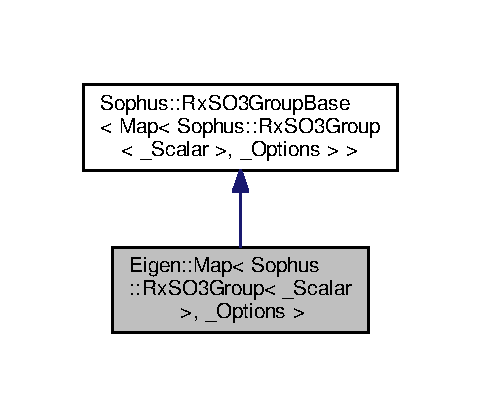
\includegraphics[width=231pt]{class_eigen_1_1_map_3_01_sophus_1_1_rx_s_o3_group_3_01___scalar_01_4_00_01___options_01_4__inherit__graph}
\end{center}
\end{figure}


Collaboration diagram for Eigen\+:\+:Map$<$ Sophus\+:\+:Rx\+S\+O3\+Group$<$ \+\_\+\+Scalar $>$, \+\_\+\+Options $>$\+:
\nopagebreak
\begin{figure}[H]
\begin{center}
\leavevmode
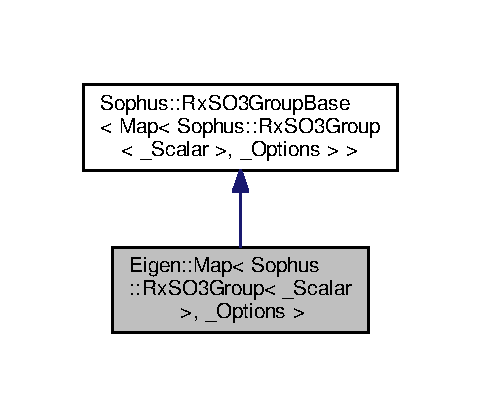
\includegraphics[width=231pt]{class_eigen_1_1_map_3_01_sophus_1_1_rx_s_o3_group_3_01___scalar_01_4_00_01___options_01_4__coll__graph}
\end{center}
\end{figure}
\subsection*{Public Types}
\begin{DoxyCompactItemize}
\item 
typedef internal\+::traits$<$ Map $>$\+::\hyperlink{class_eigen_1_1_map_3_01_sophus_1_1_rx_s_o3_group_3_01___scalar_01_4_00_01___options_01_4_a7810f1290abcedb01ffc558ddef2484f}{Scalar} \hyperlink{class_eigen_1_1_map_3_01_sophus_1_1_rx_s_o3_group_3_01___scalar_01_4_00_01___options_01_4_a7810f1290abcedb01ffc558ddef2484f}{Scalar}\hypertarget{class_eigen_1_1_map_3_01_sophus_1_1_rx_s_o3_group_3_01___scalar_01_4_00_01___options_01_4_a7810f1290abcedb01ffc558ddef2484f}{}\label{class_eigen_1_1_map_3_01_sophus_1_1_rx_s_o3_group_3_01___scalar_01_4_00_01___options_01_4_a7810f1290abcedb01ffc558ddef2484f}

\begin{DoxyCompactList}\small\item\em scalar type \end{DoxyCompactList}\item 
typedef internal\+::traits$<$ Map $>$\+::Quaternion\+Type \& \hyperlink{class_eigen_1_1_map_3_01_sophus_1_1_rx_s_o3_group_3_01___scalar_01_4_00_01___options_01_4_a01177f5e76c76c682e092fa794a5ae15}{Quaternion\+Reference}\hypertarget{class_eigen_1_1_map_3_01_sophus_1_1_rx_s_o3_group_3_01___scalar_01_4_00_01___options_01_4_a01177f5e76c76c682e092fa794a5ae15}{}\label{class_eigen_1_1_map_3_01_sophus_1_1_rx_s_o3_group_3_01___scalar_01_4_00_01___options_01_4_a01177f5e76c76c682e092fa794a5ae15}

\begin{DoxyCompactList}\small\item\em quaternion reference type \end{DoxyCompactList}\item 
typedef const internal\+::traits$<$ Map $>$\+::Quaternion\+Type \& \hyperlink{class_eigen_1_1_map_3_01_sophus_1_1_rx_s_o3_group_3_01___scalar_01_4_00_01___options_01_4_a02c1dbb3516a5492fab49f7aeb74b264}{Const\+Quaternion\+Reference}\hypertarget{class_eigen_1_1_map_3_01_sophus_1_1_rx_s_o3_group_3_01___scalar_01_4_00_01___options_01_4_a02c1dbb3516a5492fab49f7aeb74b264}{}\label{class_eigen_1_1_map_3_01_sophus_1_1_rx_s_o3_group_3_01___scalar_01_4_00_01___options_01_4_a02c1dbb3516a5492fab49f7aeb74b264}

\begin{DoxyCompactList}\small\item\em quaternion const reference type \end{DoxyCompactList}\item 
typedef \hyperlink{class_sophus_1_1_rx_s_o3_group_base_a60b2d8cd20692d3d39e5e7c729d95145}{Base\+::\+Transformation} \hyperlink{class_eigen_1_1_map_3_01_sophus_1_1_rx_s_o3_group_3_01___scalar_01_4_00_01___options_01_4_a2647ff9bb47ba1f5c7e4d15c3c9a298e}{Transformation}\hypertarget{class_eigen_1_1_map_3_01_sophus_1_1_rx_s_o3_group_3_01___scalar_01_4_00_01___options_01_4_a2647ff9bb47ba1f5c7e4d15c3c9a298e}{}\label{class_eigen_1_1_map_3_01_sophus_1_1_rx_s_o3_group_3_01___scalar_01_4_00_01___options_01_4_a2647ff9bb47ba1f5c7e4d15c3c9a298e}

\begin{DoxyCompactList}\small\item\em group transfomation type \end{DoxyCompactList}\item 
typedef \hyperlink{class_sophus_1_1_rx_s_o3_group_base_ad2d1b35ab03f6e91a80c2e78f07114a0}{Base\+::\+Point} \hyperlink{class_eigen_1_1_map_3_01_sophus_1_1_rx_s_o3_group_3_01___scalar_01_4_00_01___options_01_4_a75b1794b709e6fd66e27881ebb0a1f66}{Point}\hypertarget{class_eigen_1_1_map_3_01_sophus_1_1_rx_s_o3_group_3_01___scalar_01_4_00_01___options_01_4_a75b1794b709e6fd66e27881ebb0a1f66}{}\label{class_eigen_1_1_map_3_01_sophus_1_1_rx_s_o3_group_3_01___scalar_01_4_00_01___options_01_4_a75b1794b709e6fd66e27881ebb0a1f66}

\begin{DoxyCompactList}\small\item\em point type \end{DoxyCompactList}\item 
typedef \hyperlink{class_sophus_1_1_rx_s_o3_group_base_aa1c4034b0a69496b28f1e81fdc7510c5}{Base\+::\+Tangent} \hyperlink{class_eigen_1_1_map_3_01_sophus_1_1_rx_s_o3_group_3_01___scalar_01_4_00_01___options_01_4_aae5c72083e9b65ff5afc09b5a3336437}{Tangent}\hypertarget{class_eigen_1_1_map_3_01_sophus_1_1_rx_s_o3_group_3_01___scalar_01_4_00_01___options_01_4_aae5c72083e9b65ff5afc09b5a3336437}{}\label{class_eigen_1_1_map_3_01_sophus_1_1_rx_s_o3_group_3_01___scalar_01_4_00_01___options_01_4_aae5c72083e9b65ff5afc09b5a3336437}

\begin{DoxyCompactList}\small\item\em tangent vector type \end{DoxyCompactList}\item 
typedef \hyperlink{class_sophus_1_1_rx_s_o3_group_base_a3f7cc9982043bf0082b7946f566a8179}{Base\+::\+Adjoint} \hyperlink{class_eigen_1_1_map_3_01_sophus_1_1_rx_s_o3_group_3_01___scalar_01_4_00_01___options_01_4_a60ddaa5d46f64469fa28e625917fde1c}{Adjoint}\hypertarget{class_eigen_1_1_map_3_01_sophus_1_1_rx_s_o3_group_3_01___scalar_01_4_00_01___options_01_4_a60ddaa5d46f64469fa28e625917fde1c}{}\label{class_eigen_1_1_map_3_01_sophus_1_1_rx_s_o3_group_3_01___scalar_01_4_00_01___options_01_4_a60ddaa5d46f64469fa28e625917fde1c}

\begin{DoxyCompactList}\small\item\em adjoint transformation type \end{DoxyCompactList}\end{DoxyCompactItemize}
\subsection*{Public Member Functions}
\begin{DoxyCompactItemize}
\item 
E\+I\+G\+E\+N\+\_\+\+S\+T\+R\+O\+N\+G\+\_\+\+I\+N\+L\+I\+NE {\bfseries Map} (\hyperlink{class_eigen_1_1_map_3_01_sophus_1_1_rx_s_o3_group_3_01___scalar_01_4_00_01___options_01_4_a7810f1290abcedb01ffc558ddef2484f}{Scalar} $\ast$coeffs)\hypertarget{class_eigen_1_1_map_3_01_sophus_1_1_rx_s_o3_group_3_01___scalar_01_4_00_01___options_01_4_a927226af907a202897f12382a5cde67e}{}\label{class_eigen_1_1_map_3_01_sophus_1_1_rx_s_o3_group_3_01___scalar_01_4_00_01___options_01_4_a927226af907a202897f12382a5cde67e}

\item 
E\+I\+G\+E\+N\+\_\+\+S\+T\+R\+O\+N\+G\+\_\+\+I\+N\+L\+I\+NE \hyperlink{class_eigen_1_1_map_3_01_sophus_1_1_rx_s_o3_group_3_01___scalar_01_4_00_01___options_01_4_a01177f5e76c76c682e092fa794a5ae15}{Quaternion\+Reference} \hyperlink{class_eigen_1_1_map_3_01_sophus_1_1_rx_s_o3_group_3_01___scalar_01_4_00_01___options_01_4_ae78ec49b1edafe71ccf199f24a9e251b}{quaternion} ()\hypertarget{class_eigen_1_1_map_3_01_sophus_1_1_rx_s_o3_group_3_01___scalar_01_4_00_01___options_01_4_ae78ec49b1edafe71ccf199f24a9e251b}{}\label{class_eigen_1_1_map_3_01_sophus_1_1_rx_s_o3_group_3_01___scalar_01_4_00_01___options_01_4_ae78ec49b1edafe71ccf199f24a9e251b}

\begin{DoxyCompactList}\small\item\em Mutator of quaternion. \end{DoxyCompactList}\item 
E\+I\+G\+E\+N\+\_\+\+S\+T\+R\+O\+N\+G\+\_\+\+I\+N\+L\+I\+NE \hyperlink{class_eigen_1_1_map_3_01_sophus_1_1_rx_s_o3_group_3_01___scalar_01_4_00_01___options_01_4_a02c1dbb3516a5492fab49f7aeb74b264}{Const\+Quaternion\+Reference} \hyperlink{class_eigen_1_1_map_3_01_sophus_1_1_rx_s_o3_group_3_01___scalar_01_4_00_01___options_01_4_a4c5dcaf4155bcdc964ea8bd8b461d8f2}{quaternion} () const \hypertarget{class_eigen_1_1_map_3_01_sophus_1_1_rx_s_o3_group_3_01___scalar_01_4_00_01___options_01_4_a4c5dcaf4155bcdc964ea8bd8b461d8f2}{}\label{class_eigen_1_1_map_3_01_sophus_1_1_rx_s_o3_group_3_01___scalar_01_4_00_01___options_01_4_a4c5dcaf4155bcdc964ea8bd8b461d8f2}

\begin{DoxyCompactList}\small\item\em Accessor of quaternion. \end{DoxyCompactList}\end{DoxyCompactItemize}
\subsection*{Static Public Attributes}
\begin{DoxyCompactItemize}
\item 
static const int \hyperlink{class_eigen_1_1_map_3_01_sophus_1_1_rx_s_o3_group_3_01___scalar_01_4_00_01___options_01_4_a6953c55e948ee44bd05acc150caefd90}{DoF} = Base\+::\+DoF\hypertarget{class_eigen_1_1_map_3_01_sophus_1_1_rx_s_o3_group_3_01___scalar_01_4_00_01___options_01_4_a6953c55e948ee44bd05acc150caefd90}{}\label{class_eigen_1_1_map_3_01_sophus_1_1_rx_s_o3_group_3_01___scalar_01_4_00_01___options_01_4_a6953c55e948ee44bd05acc150caefd90}

\begin{DoxyCompactList}\small\item\em degree of freedom of group \end{DoxyCompactList}\item 
static const int \hyperlink{class_eigen_1_1_map_3_01_sophus_1_1_rx_s_o3_group_3_01___scalar_01_4_00_01___options_01_4_ad4a0815abf66577dc103a9fa652e88a6}{num\+\_\+parameters} = Base\+::num\+\_\+parameters\hypertarget{class_eigen_1_1_map_3_01_sophus_1_1_rx_s_o3_group_3_01___scalar_01_4_00_01___options_01_4_ad4a0815abf66577dc103a9fa652e88a6}{}\label{class_eigen_1_1_map_3_01_sophus_1_1_rx_s_o3_group_3_01___scalar_01_4_00_01___options_01_4_ad4a0815abf66577dc103a9fa652e88a6}

\begin{DoxyCompactList}\small\item\em number of internal parameters used \end{DoxyCompactList}\item 
static const int \hyperlink{class_eigen_1_1_map_3_01_sophus_1_1_rx_s_o3_group_3_01___scalar_01_4_00_01___options_01_4_a61464d6593d4fdd5dbd8a6591b8d9686}{N} = Base\+::N\hypertarget{class_eigen_1_1_map_3_01_sophus_1_1_rx_s_o3_group_3_01___scalar_01_4_00_01___options_01_4_a61464d6593d4fdd5dbd8a6591b8d9686}{}\label{class_eigen_1_1_map_3_01_sophus_1_1_rx_s_o3_group_3_01___scalar_01_4_00_01___options_01_4_a61464d6593d4fdd5dbd8a6591b8d9686}

\begin{DoxyCompactList}\small\item\em group transformations are NxN matrices \end{DoxyCompactList}\end{DoxyCompactItemize}
\subsection*{Protected Attributes}
\begin{DoxyCompactItemize}
\item 
Map$<$ Quaternion$<$ \hyperlink{class_eigen_1_1_map_3_01_sophus_1_1_rx_s_o3_group_3_01___scalar_01_4_00_01___options_01_4_a7810f1290abcedb01ffc558ddef2484f}{Scalar} $>$, \+\_\+\+Options $>$ {\bfseries quaternion\+\_\+}\hypertarget{class_eigen_1_1_map_3_01_sophus_1_1_rx_s_o3_group_3_01___scalar_01_4_00_01___options_01_4_a39dc0a1f07c9aa8f4ac51dc4c5ae9634}{}\label{class_eigen_1_1_map_3_01_sophus_1_1_rx_s_o3_group_3_01___scalar_01_4_00_01___options_01_4_a39dc0a1f07c9aa8f4ac51dc4c5ae9634}

\end{DoxyCompactItemize}
\subsection*{Additional Inherited Members}


\subsection{Detailed Description}
\subsubsection*{template$<$typename \+\_\+\+Scalar, int \+\_\+\+Options$>$\\*
class Eigen\+::\+Map$<$ Sophus\+::\+Rx\+S\+O3\+Group$<$ \+\_\+\+Scalar $>$, \+\_\+\+Options $>$}

Specialisation of Eigen\+::\+Map for Rx\+S\+O3\+Group\+Base. 

Allows us to wrap Rx\+S\+O3 Objects around P\+OD array (e.\+g. external c style quaternion) 

Definition at line 720 of file rxso3.\+hpp.



The documentation for this class was generated from the following file\+:\begin{DoxyCompactItemize}
\item 
include/\+Sophus/sophus/rxso3.\+hpp\end{DoxyCompactItemize}

\hypertarget{class_eigen_1_1_map_3_01_sophus_1_1_s_e2_group_3_01___scalar_01_4_00_01___options_01_4}{}\section{Eigen\+:\+:Map$<$ Sophus\+:\+:S\+E2\+Group$<$ \+\_\+\+Scalar $>$, \+\_\+\+Options $>$ Class Template Reference}
\label{class_eigen_1_1_map_3_01_sophus_1_1_s_e2_group_3_01___scalar_01_4_00_01___options_01_4}\index{Eigen\+::\+Map$<$ Sophus\+::\+S\+E2\+Group$<$ \+\_\+\+Scalar $>$, \+\_\+\+Options $>$@{Eigen\+::\+Map$<$ Sophus\+::\+S\+E2\+Group$<$ \+\_\+\+Scalar $>$, \+\_\+\+Options $>$}}


Specialisation of Eigen\+::\+Map for S\+E2\+Group\+Base.  




{\ttfamily \#include $<$se2.\+hpp$>$}



Inheritance diagram for Eigen\+:\+:Map$<$ Sophus\+:\+:S\+E2\+Group$<$ \+\_\+\+Scalar $>$, \+\_\+\+Options $>$\+:
\nopagebreak
\begin{figure}[H]
\begin{center}
\leavevmode
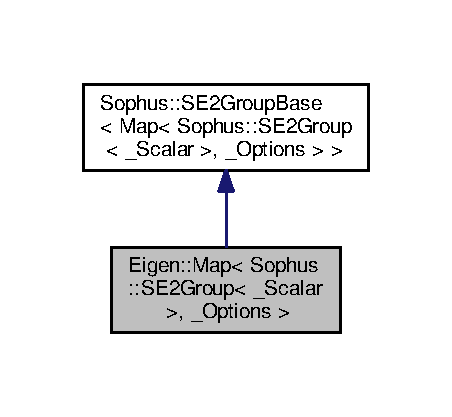
\includegraphics[width=217pt]{class_eigen_1_1_map_3_01_sophus_1_1_s_e2_group_3_01___scalar_01_4_00_01___options_01_4__inherit__graph}
\end{center}
\end{figure}


Collaboration diagram for Eigen\+:\+:Map$<$ Sophus\+:\+:S\+E2\+Group$<$ \+\_\+\+Scalar $>$, \+\_\+\+Options $>$\+:
\nopagebreak
\begin{figure}[H]
\begin{center}
\leavevmode
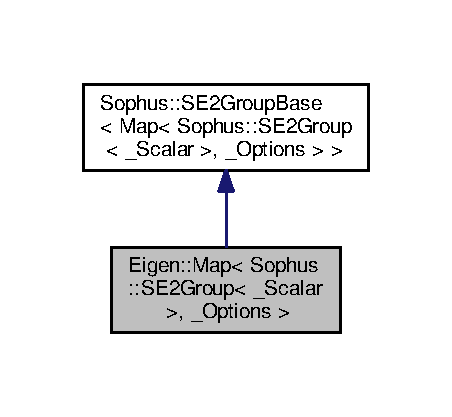
\includegraphics[width=217pt]{class_eigen_1_1_map_3_01_sophus_1_1_s_e2_group_3_01___scalar_01_4_00_01___options_01_4__coll__graph}
\end{center}
\end{figure}
\subsection*{Public Types}
\begin{DoxyCompactItemize}
\item 
typedef internal\+::traits$<$ Map $>$\+::\hyperlink{class_eigen_1_1_map_3_01_sophus_1_1_s_e2_group_3_01___scalar_01_4_00_01___options_01_4_a786250298fc0362636d913ce5b96894c}{Scalar} \hyperlink{class_eigen_1_1_map_3_01_sophus_1_1_s_e2_group_3_01___scalar_01_4_00_01___options_01_4_a786250298fc0362636d913ce5b96894c}{Scalar}\hypertarget{class_eigen_1_1_map_3_01_sophus_1_1_s_e2_group_3_01___scalar_01_4_00_01___options_01_4_a786250298fc0362636d913ce5b96894c}{}\label{class_eigen_1_1_map_3_01_sophus_1_1_s_e2_group_3_01___scalar_01_4_00_01___options_01_4_a786250298fc0362636d913ce5b96894c}

\begin{DoxyCompactList}\small\item\em scalar type \end{DoxyCompactList}\item 
typedef internal\+::traits$<$ Map $>$\+::Translation\+Type \& \hyperlink{class_eigen_1_1_map_3_01_sophus_1_1_s_e2_group_3_01___scalar_01_4_00_01___options_01_4_a7d845300d37b519b0730cc5ac098f2f2}{Translation\+Reference}\hypertarget{class_eigen_1_1_map_3_01_sophus_1_1_s_e2_group_3_01___scalar_01_4_00_01___options_01_4_a7d845300d37b519b0730cc5ac098f2f2}{}\label{class_eigen_1_1_map_3_01_sophus_1_1_s_e2_group_3_01___scalar_01_4_00_01___options_01_4_a7d845300d37b519b0730cc5ac098f2f2}

\begin{DoxyCompactList}\small\item\em translation reference type \end{DoxyCompactList}\item 
typedef const internal\+::traits$<$ Map $>$\+::Translation\+Type \& \hyperlink{class_eigen_1_1_map_3_01_sophus_1_1_s_e2_group_3_01___scalar_01_4_00_01___options_01_4_ab7bffb4711a188629b17ae3cb3c03a49}{Const\+Translation\+Reference}\hypertarget{class_eigen_1_1_map_3_01_sophus_1_1_s_e2_group_3_01___scalar_01_4_00_01___options_01_4_ab7bffb4711a188629b17ae3cb3c03a49}{}\label{class_eigen_1_1_map_3_01_sophus_1_1_s_e2_group_3_01___scalar_01_4_00_01___options_01_4_ab7bffb4711a188629b17ae3cb3c03a49}

\begin{DoxyCompactList}\small\item\em translation reference type \end{DoxyCompactList}\item 
typedef internal\+::traits$<$ Map $>$\+::S\+O2\+Type \& \hyperlink{class_eigen_1_1_map_3_01_sophus_1_1_s_e2_group_3_01___scalar_01_4_00_01___options_01_4_aa02197afddb3c3f212fa6f89b19aea6c}{S\+O2\+Reference}\hypertarget{class_eigen_1_1_map_3_01_sophus_1_1_s_e2_group_3_01___scalar_01_4_00_01___options_01_4_aa02197afddb3c3f212fa6f89b19aea6c}{}\label{class_eigen_1_1_map_3_01_sophus_1_1_s_e2_group_3_01___scalar_01_4_00_01___options_01_4_aa02197afddb3c3f212fa6f89b19aea6c}

\begin{DoxyCompactList}\small\item\em S\+O2 reference type. \end{DoxyCompactList}\item 
typedef const internal\+::traits$<$ Map $>$\+::S\+O2\+Type \& \hyperlink{class_eigen_1_1_map_3_01_sophus_1_1_s_e2_group_3_01___scalar_01_4_00_01___options_01_4_a95a0f0d5cfa5b98c73129061e9f895eb}{Const\+S\+O2\+Reference}\hypertarget{class_eigen_1_1_map_3_01_sophus_1_1_s_e2_group_3_01___scalar_01_4_00_01___options_01_4_a95a0f0d5cfa5b98c73129061e9f895eb}{}\label{class_eigen_1_1_map_3_01_sophus_1_1_s_e2_group_3_01___scalar_01_4_00_01___options_01_4_a95a0f0d5cfa5b98c73129061e9f895eb}

\begin{DoxyCompactList}\small\item\em S\+O2 const reference type. \end{DoxyCompactList}\item 
typedef \hyperlink{class_sophus_1_1_s_e2_group_base_a82fe531d4b64813525d4ebd131da9bcd}{Base\+::\+Transformation} \hyperlink{class_eigen_1_1_map_3_01_sophus_1_1_s_e2_group_3_01___scalar_01_4_00_01___options_01_4_aa0679ea66e90d4b033fb6f8ee39353d3}{Transformation}\hypertarget{class_eigen_1_1_map_3_01_sophus_1_1_s_e2_group_3_01___scalar_01_4_00_01___options_01_4_aa0679ea66e90d4b033fb6f8ee39353d3}{}\label{class_eigen_1_1_map_3_01_sophus_1_1_s_e2_group_3_01___scalar_01_4_00_01___options_01_4_aa0679ea66e90d4b033fb6f8ee39353d3}

\begin{DoxyCompactList}\small\item\em group transfomation type \end{DoxyCompactList}\item 
typedef \hyperlink{class_sophus_1_1_s_e2_group_base_add8b024098bc6fcecdefb42229fa881b}{Base\+::\+Point} \hyperlink{class_eigen_1_1_map_3_01_sophus_1_1_s_e2_group_3_01___scalar_01_4_00_01___options_01_4_aad5a573c1e69585f2d5b54a404d83053}{Point}\hypertarget{class_eigen_1_1_map_3_01_sophus_1_1_s_e2_group_3_01___scalar_01_4_00_01___options_01_4_aad5a573c1e69585f2d5b54a404d83053}{}\label{class_eigen_1_1_map_3_01_sophus_1_1_s_e2_group_3_01___scalar_01_4_00_01___options_01_4_aad5a573c1e69585f2d5b54a404d83053}

\begin{DoxyCompactList}\small\item\em point type \end{DoxyCompactList}\item 
typedef \hyperlink{class_sophus_1_1_s_e2_group_base_a71b41e6cde48514241c7bffcbe34923f}{Base\+::\+Tangent} \hyperlink{class_eigen_1_1_map_3_01_sophus_1_1_s_e2_group_3_01___scalar_01_4_00_01___options_01_4_a0e620eca865271b3b9bcb2c75dfbf2fa}{Tangent}\hypertarget{class_eigen_1_1_map_3_01_sophus_1_1_s_e2_group_3_01___scalar_01_4_00_01___options_01_4_a0e620eca865271b3b9bcb2c75dfbf2fa}{}\label{class_eigen_1_1_map_3_01_sophus_1_1_s_e2_group_3_01___scalar_01_4_00_01___options_01_4_a0e620eca865271b3b9bcb2c75dfbf2fa}

\begin{DoxyCompactList}\small\item\em tangent vector type \end{DoxyCompactList}\item 
typedef \hyperlink{class_sophus_1_1_s_e2_group_base_a6e0785a6f8399456a8bd0b057bae02ee}{Base\+::\+Adjoint} \hyperlink{class_eigen_1_1_map_3_01_sophus_1_1_s_e2_group_3_01___scalar_01_4_00_01___options_01_4_aee9a710042c2e2fd28765f533b76811c}{Adjoint}\hypertarget{class_eigen_1_1_map_3_01_sophus_1_1_s_e2_group_3_01___scalar_01_4_00_01___options_01_4_aee9a710042c2e2fd28765f533b76811c}{}\label{class_eigen_1_1_map_3_01_sophus_1_1_s_e2_group_3_01___scalar_01_4_00_01___options_01_4_aee9a710042c2e2fd28765f533b76811c}

\begin{DoxyCompactList}\small\item\em adjoint transformation type \end{DoxyCompactList}\end{DoxyCompactItemize}
\subsection*{Public Member Functions}
\begin{DoxyCompactItemize}
\item 
E\+I\+G\+E\+N\+\_\+\+S\+T\+R\+O\+N\+G\+\_\+\+I\+N\+L\+I\+NE {\bfseries Map} (\hyperlink{class_eigen_1_1_map_3_01_sophus_1_1_s_e2_group_3_01___scalar_01_4_00_01___options_01_4_a786250298fc0362636d913ce5b96894c}{Scalar} $\ast$coeffs)\hypertarget{class_eigen_1_1_map_3_01_sophus_1_1_s_e2_group_3_01___scalar_01_4_00_01___options_01_4_a80fb5caf699f9d3b702beb74305850db}{}\label{class_eigen_1_1_map_3_01_sophus_1_1_s_e2_group_3_01___scalar_01_4_00_01___options_01_4_a80fb5caf699f9d3b702beb74305850db}

\item 
E\+I\+G\+E\+N\+\_\+\+S\+T\+R\+O\+N\+G\+\_\+\+I\+N\+L\+I\+NE \hyperlink{class_eigen_1_1_map_3_01_sophus_1_1_s_e2_group_3_01___scalar_01_4_00_01___options_01_4_aa02197afddb3c3f212fa6f89b19aea6c}{S\+O2\+Reference} \hyperlink{class_eigen_1_1_map_3_01_sophus_1_1_s_e2_group_3_01___scalar_01_4_00_01___options_01_4_a314b3a4f182ea1d0c7d0008c01dedc82}{so2} ()\hypertarget{class_eigen_1_1_map_3_01_sophus_1_1_s_e2_group_3_01___scalar_01_4_00_01___options_01_4_a314b3a4f182ea1d0c7d0008c01dedc82}{}\label{class_eigen_1_1_map_3_01_sophus_1_1_s_e2_group_3_01___scalar_01_4_00_01___options_01_4_a314b3a4f182ea1d0c7d0008c01dedc82}

\begin{DoxyCompactList}\small\item\em Mutator of S\+O2. \end{DoxyCompactList}\item 
E\+I\+G\+E\+N\+\_\+\+S\+T\+R\+O\+N\+G\+\_\+\+I\+N\+L\+I\+NE \hyperlink{class_eigen_1_1_map_3_01_sophus_1_1_s_e2_group_3_01___scalar_01_4_00_01___options_01_4_a95a0f0d5cfa5b98c73129061e9f895eb}{Const\+S\+O2\+Reference} \hyperlink{class_eigen_1_1_map_3_01_sophus_1_1_s_e2_group_3_01___scalar_01_4_00_01___options_01_4_a156fff192dd64054612fc525dc86b57d}{so2} () const \hypertarget{class_eigen_1_1_map_3_01_sophus_1_1_s_e2_group_3_01___scalar_01_4_00_01___options_01_4_a156fff192dd64054612fc525dc86b57d}{}\label{class_eigen_1_1_map_3_01_sophus_1_1_s_e2_group_3_01___scalar_01_4_00_01___options_01_4_a156fff192dd64054612fc525dc86b57d}

\begin{DoxyCompactList}\small\item\em Accessor of S\+O2. \end{DoxyCompactList}\item 
E\+I\+G\+E\+N\+\_\+\+S\+T\+R\+O\+N\+G\+\_\+\+I\+N\+L\+I\+NE \hyperlink{class_eigen_1_1_map_3_01_sophus_1_1_s_e2_group_3_01___scalar_01_4_00_01___options_01_4_a7d845300d37b519b0730cc5ac098f2f2}{Translation\+Reference} \hyperlink{class_eigen_1_1_map_3_01_sophus_1_1_s_e2_group_3_01___scalar_01_4_00_01___options_01_4_a72a936f1dc0808e14b2cbb21ae3835ef}{translation} ()\hypertarget{class_eigen_1_1_map_3_01_sophus_1_1_s_e2_group_3_01___scalar_01_4_00_01___options_01_4_a72a936f1dc0808e14b2cbb21ae3835ef}{}\label{class_eigen_1_1_map_3_01_sophus_1_1_s_e2_group_3_01___scalar_01_4_00_01___options_01_4_a72a936f1dc0808e14b2cbb21ae3835ef}

\begin{DoxyCompactList}\small\item\em Mutator of translation vector. \end{DoxyCompactList}\item 
E\+I\+G\+E\+N\+\_\+\+S\+T\+R\+O\+N\+G\+\_\+\+I\+N\+L\+I\+NE \hyperlink{class_eigen_1_1_map_3_01_sophus_1_1_s_e2_group_3_01___scalar_01_4_00_01___options_01_4_ab7bffb4711a188629b17ae3cb3c03a49}{Const\+Translation\+Reference} \hyperlink{class_eigen_1_1_map_3_01_sophus_1_1_s_e2_group_3_01___scalar_01_4_00_01___options_01_4_a7619bfeaf0e0c601d84b8fcb2f584569}{translation} () const \hypertarget{class_eigen_1_1_map_3_01_sophus_1_1_s_e2_group_3_01___scalar_01_4_00_01___options_01_4_a7619bfeaf0e0c601d84b8fcb2f584569}{}\label{class_eigen_1_1_map_3_01_sophus_1_1_s_e2_group_3_01___scalar_01_4_00_01___options_01_4_a7619bfeaf0e0c601d84b8fcb2f584569}

\begin{DoxyCompactList}\small\item\em Accessor of translation vector. \end{DoxyCompactList}\end{DoxyCompactItemize}
\subsection*{Static Public Attributes}
\begin{DoxyCompactItemize}
\item 
static const int \hyperlink{class_eigen_1_1_map_3_01_sophus_1_1_s_e2_group_3_01___scalar_01_4_00_01___options_01_4_a6a6cdf931e55ebedbd290bea11d4a8a6}{DoF} = Base\+::\+DoF\hypertarget{class_eigen_1_1_map_3_01_sophus_1_1_s_e2_group_3_01___scalar_01_4_00_01___options_01_4_a6a6cdf931e55ebedbd290bea11d4a8a6}{}\label{class_eigen_1_1_map_3_01_sophus_1_1_s_e2_group_3_01___scalar_01_4_00_01___options_01_4_a6a6cdf931e55ebedbd290bea11d4a8a6}

\begin{DoxyCompactList}\small\item\em degree of freedom of group \end{DoxyCompactList}\item 
static const int \hyperlink{class_eigen_1_1_map_3_01_sophus_1_1_s_e2_group_3_01___scalar_01_4_00_01___options_01_4_a3862446f8d422244b8a1ac11871184fc}{num\+\_\+parameters} = Base\+::num\+\_\+parameters\hypertarget{class_eigen_1_1_map_3_01_sophus_1_1_s_e2_group_3_01___scalar_01_4_00_01___options_01_4_a3862446f8d422244b8a1ac11871184fc}{}\label{class_eigen_1_1_map_3_01_sophus_1_1_s_e2_group_3_01___scalar_01_4_00_01___options_01_4_a3862446f8d422244b8a1ac11871184fc}

\begin{DoxyCompactList}\small\item\em number of internal parameters used \end{DoxyCompactList}\item 
static const int \hyperlink{class_eigen_1_1_map_3_01_sophus_1_1_s_e2_group_3_01___scalar_01_4_00_01___options_01_4_aa94644b24bd2c93bdc532852b86a338c}{N} = Base\+::N\hypertarget{class_eigen_1_1_map_3_01_sophus_1_1_s_e2_group_3_01___scalar_01_4_00_01___options_01_4_aa94644b24bd2c93bdc532852b86a338c}{}\label{class_eigen_1_1_map_3_01_sophus_1_1_s_e2_group_3_01___scalar_01_4_00_01___options_01_4_aa94644b24bd2c93bdc532852b86a338c}

\begin{DoxyCompactList}\small\item\em group transformations are NxN matrices \end{DoxyCompactList}\end{DoxyCompactItemize}
\subsection*{Protected Attributes}
\begin{DoxyCompactItemize}
\item 
Map$<$ \hyperlink{class_sophus_1_1_s_o2_group}{Sophus\+::\+S\+O2\+Group}$<$ \hyperlink{class_eigen_1_1_map_3_01_sophus_1_1_s_e2_group_3_01___scalar_01_4_00_01___options_01_4_a786250298fc0362636d913ce5b96894c}{Scalar} $>$, \+\_\+\+Options $>$ {\bfseries so2\+\_\+}\hypertarget{class_eigen_1_1_map_3_01_sophus_1_1_s_e2_group_3_01___scalar_01_4_00_01___options_01_4_a97405ec3cd86e6d5eab7af7cc2bb537e}{}\label{class_eigen_1_1_map_3_01_sophus_1_1_s_e2_group_3_01___scalar_01_4_00_01___options_01_4_a97405ec3cd86e6d5eab7af7cc2bb537e}

\item 
Map$<$ Matrix$<$ \hyperlink{class_eigen_1_1_map_3_01_sophus_1_1_s_e2_group_3_01___scalar_01_4_00_01___options_01_4_a786250298fc0362636d913ce5b96894c}{Scalar}, 2, 1 $>$, \+\_\+\+Options $>$ {\bfseries translation\+\_\+}\hypertarget{class_eigen_1_1_map_3_01_sophus_1_1_s_e2_group_3_01___scalar_01_4_00_01___options_01_4_ab015eab7c1800ae8fb80790caf547481}{}\label{class_eigen_1_1_map_3_01_sophus_1_1_s_e2_group_3_01___scalar_01_4_00_01___options_01_4_ab015eab7c1800ae8fb80790caf547481}

\end{DoxyCompactItemize}
\subsection*{Additional Inherited Members}


\subsection{Detailed Description}
\subsubsection*{template$<$typename \+\_\+\+Scalar, int \+\_\+\+Options$>$\\*
class Eigen\+::\+Map$<$ Sophus\+::\+S\+E2\+Group$<$ \+\_\+\+Scalar $>$, \+\_\+\+Options $>$}

Specialisation of Eigen\+::\+Map for S\+E2\+Group\+Base. 

Allows us to wrap S\+E2 Objects around P\+OD array (e.\+g. external c style complex) 

Definition at line 751 of file se2.\+hpp.



The documentation for this class was generated from the following file\+:\begin{DoxyCompactItemize}
\item 
include/\+Sophus/sophus/se2.\+hpp\end{DoxyCompactItemize}

\hypertarget{class_eigen_1_1_map_3_01_sophus_1_1_s_e3_group_3_01___scalar_01_4_00_01___options_01_4}{}\section{Eigen\+:\+:Map$<$ Sophus\+:\+:S\+E3\+Group$<$ \+\_\+\+Scalar $>$, \+\_\+\+Options $>$ Class Template Reference}
\label{class_eigen_1_1_map_3_01_sophus_1_1_s_e3_group_3_01___scalar_01_4_00_01___options_01_4}\index{Eigen\+::\+Map$<$ Sophus\+::\+S\+E3\+Group$<$ \+\_\+\+Scalar $>$, \+\_\+\+Options $>$@{Eigen\+::\+Map$<$ Sophus\+::\+S\+E3\+Group$<$ \+\_\+\+Scalar $>$, \+\_\+\+Options $>$}}


Specialisation of Eigen\+::\+Map for S\+E3\+Group\+Base.  




{\ttfamily \#include $<$se3.\+hpp$>$}



Inheritance diagram for Eigen\+:\+:Map$<$ Sophus\+:\+:S\+E3\+Group$<$ \+\_\+\+Scalar $>$, \+\_\+\+Options $>$\+:
\nopagebreak
\begin{figure}[H]
\begin{center}
\leavevmode
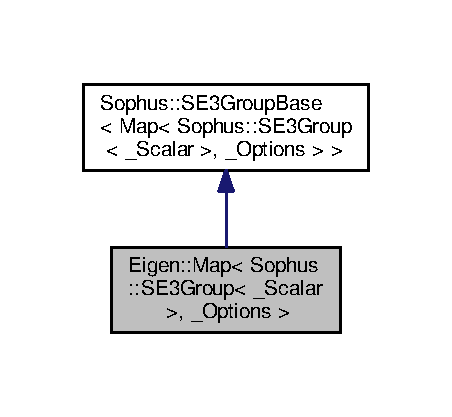
\includegraphics[width=217pt]{class_eigen_1_1_map_3_01_sophus_1_1_s_e3_group_3_01___scalar_01_4_00_01___options_01_4__inherit__graph}
\end{center}
\end{figure}


Collaboration diagram for Eigen\+:\+:Map$<$ Sophus\+:\+:S\+E3\+Group$<$ \+\_\+\+Scalar $>$, \+\_\+\+Options $>$\+:
\nopagebreak
\begin{figure}[H]
\begin{center}
\leavevmode
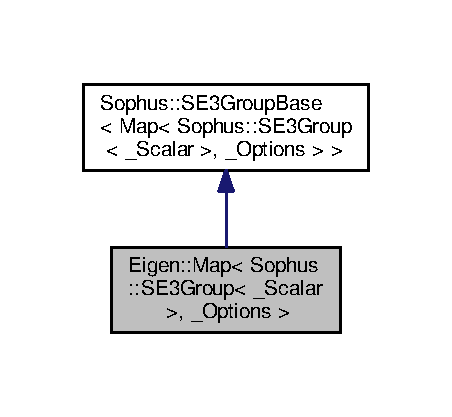
\includegraphics[width=217pt]{class_eigen_1_1_map_3_01_sophus_1_1_s_e3_group_3_01___scalar_01_4_00_01___options_01_4__coll__graph}
\end{center}
\end{figure}
\subsection*{Public Types}
\begin{DoxyCompactItemize}
\item 
typedef internal\+::traits$<$ Map $>$\+::\hyperlink{class_eigen_1_1_map_3_01_sophus_1_1_s_e3_group_3_01___scalar_01_4_00_01___options_01_4_a09d0d1676e19353b9b474da1e5e9df2c}{Scalar} \hyperlink{class_eigen_1_1_map_3_01_sophus_1_1_s_e3_group_3_01___scalar_01_4_00_01___options_01_4_a09d0d1676e19353b9b474da1e5e9df2c}{Scalar}\hypertarget{class_eigen_1_1_map_3_01_sophus_1_1_s_e3_group_3_01___scalar_01_4_00_01___options_01_4_a09d0d1676e19353b9b474da1e5e9df2c}{}\label{class_eigen_1_1_map_3_01_sophus_1_1_s_e3_group_3_01___scalar_01_4_00_01___options_01_4_a09d0d1676e19353b9b474da1e5e9df2c}

\begin{DoxyCompactList}\small\item\em scalar type \end{DoxyCompactList}\item 
typedef internal\+::traits$<$ Map $>$\+::Translation\+Type \& \hyperlink{class_eigen_1_1_map_3_01_sophus_1_1_s_e3_group_3_01___scalar_01_4_00_01___options_01_4_a02744f35b5be16827bff99971a171e02}{Translation\+Reference}\hypertarget{class_eigen_1_1_map_3_01_sophus_1_1_s_e3_group_3_01___scalar_01_4_00_01___options_01_4_a02744f35b5be16827bff99971a171e02}{}\label{class_eigen_1_1_map_3_01_sophus_1_1_s_e3_group_3_01___scalar_01_4_00_01___options_01_4_a02744f35b5be16827bff99971a171e02}

\begin{DoxyCompactList}\small\item\em translation reference type \end{DoxyCompactList}\item 
typedef const internal\+::traits$<$ Map $>$\+::Translation\+Type \& \hyperlink{class_eigen_1_1_map_3_01_sophus_1_1_s_e3_group_3_01___scalar_01_4_00_01___options_01_4_af4ec7e66b89c09a78c6290b0f3fbd747}{Const\+Translation\+Reference}\hypertarget{class_eigen_1_1_map_3_01_sophus_1_1_s_e3_group_3_01___scalar_01_4_00_01___options_01_4_af4ec7e66b89c09a78c6290b0f3fbd747}{}\label{class_eigen_1_1_map_3_01_sophus_1_1_s_e3_group_3_01___scalar_01_4_00_01___options_01_4_af4ec7e66b89c09a78c6290b0f3fbd747}

\begin{DoxyCompactList}\small\item\em translation const reference type \end{DoxyCompactList}\item 
typedef internal\+::traits$<$ Map $>$\+::S\+O3\+Type \& \hyperlink{class_eigen_1_1_map_3_01_sophus_1_1_s_e3_group_3_01___scalar_01_4_00_01___options_01_4_a8847044218603f949618d62e714481e0}{S\+O3\+Reference}\hypertarget{class_eigen_1_1_map_3_01_sophus_1_1_s_e3_group_3_01___scalar_01_4_00_01___options_01_4_a8847044218603f949618d62e714481e0}{}\label{class_eigen_1_1_map_3_01_sophus_1_1_s_e3_group_3_01___scalar_01_4_00_01___options_01_4_a8847044218603f949618d62e714481e0}

\begin{DoxyCompactList}\small\item\em S\+O3 reference type. \end{DoxyCompactList}\item 
typedef const internal\+::traits$<$ Map $>$\+::S\+O3\+Type \& \hyperlink{class_eigen_1_1_map_3_01_sophus_1_1_s_e3_group_3_01___scalar_01_4_00_01___options_01_4_ae5d42a314a260ccc1240218a47b99f94}{Const\+S\+O3\+Reference}\hypertarget{class_eigen_1_1_map_3_01_sophus_1_1_s_e3_group_3_01___scalar_01_4_00_01___options_01_4_ae5d42a314a260ccc1240218a47b99f94}{}\label{class_eigen_1_1_map_3_01_sophus_1_1_s_e3_group_3_01___scalar_01_4_00_01___options_01_4_ae5d42a314a260ccc1240218a47b99f94}

\begin{DoxyCompactList}\small\item\em S\+O3 const reference type. \end{DoxyCompactList}\item 
typedef \hyperlink{class_sophus_1_1_s_e3_group_base_a426ebd53f324a4fd6d36c28028f967f1}{Base\+::\+Transformation} \hyperlink{class_eigen_1_1_map_3_01_sophus_1_1_s_e3_group_3_01___scalar_01_4_00_01___options_01_4_a3554c03dc5a569a9c8af6068f427af46}{Transformation}\hypertarget{class_eigen_1_1_map_3_01_sophus_1_1_s_e3_group_3_01___scalar_01_4_00_01___options_01_4_a3554c03dc5a569a9c8af6068f427af46}{}\label{class_eigen_1_1_map_3_01_sophus_1_1_s_e3_group_3_01___scalar_01_4_00_01___options_01_4_a3554c03dc5a569a9c8af6068f427af46}

\begin{DoxyCompactList}\small\item\em group transfomation type \end{DoxyCompactList}\item 
typedef \hyperlink{class_sophus_1_1_s_e3_group_base_aca2cf20e857567b74fb399c7ee76c744}{Base\+::\+Point} \hyperlink{class_eigen_1_1_map_3_01_sophus_1_1_s_e3_group_3_01___scalar_01_4_00_01___options_01_4_a7d268c6f8843b33556e7d34ee013862c}{Point}\hypertarget{class_eigen_1_1_map_3_01_sophus_1_1_s_e3_group_3_01___scalar_01_4_00_01___options_01_4_a7d268c6f8843b33556e7d34ee013862c}{}\label{class_eigen_1_1_map_3_01_sophus_1_1_s_e3_group_3_01___scalar_01_4_00_01___options_01_4_a7d268c6f8843b33556e7d34ee013862c}

\begin{DoxyCompactList}\small\item\em point type \end{DoxyCompactList}\item 
typedef \hyperlink{class_sophus_1_1_s_e3_group_base_a45f63b562f0614853cef2c04c4cd5f2b}{Base\+::\+Tangent} \hyperlink{class_eigen_1_1_map_3_01_sophus_1_1_s_e3_group_3_01___scalar_01_4_00_01___options_01_4_a8d68bc2d6d32babafa95546194c60301}{Tangent}\hypertarget{class_eigen_1_1_map_3_01_sophus_1_1_s_e3_group_3_01___scalar_01_4_00_01___options_01_4_a8d68bc2d6d32babafa95546194c60301}{}\label{class_eigen_1_1_map_3_01_sophus_1_1_s_e3_group_3_01___scalar_01_4_00_01___options_01_4_a8d68bc2d6d32babafa95546194c60301}

\begin{DoxyCompactList}\small\item\em tangent vector type \end{DoxyCompactList}\item 
typedef \hyperlink{class_sophus_1_1_s_e3_group_base_ac2e0179cb3e9490604c417d8e59a92d3}{Base\+::\+Adjoint} \hyperlink{class_eigen_1_1_map_3_01_sophus_1_1_s_e3_group_3_01___scalar_01_4_00_01___options_01_4_a32b7d1f821b82cb8c9f20a676efa286e}{Adjoint}\hypertarget{class_eigen_1_1_map_3_01_sophus_1_1_s_e3_group_3_01___scalar_01_4_00_01___options_01_4_a32b7d1f821b82cb8c9f20a676efa286e}{}\label{class_eigen_1_1_map_3_01_sophus_1_1_s_e3_group_3_01___scalar_01_4_00_01___options_01_4_a32b7d1f821b82cb8c9f20a676efa286e}

\begin{DoxyCompactList}\small\item\em adjoint transformation type \end{DoxyCompactList}\end{DoxyCompactItemize}
\subsection*{Public Member Functions}
\begin{DoxyCompactItemize}
\item 
E\+I\+G\+E\+N\+\_\+\+S\+T\+R\+O\+N\+G\+\_\+\+I\+N\+L\+I\+NE {\bfseries Map} (\hyperlink{class_eigen_1_1_map_3_01_sophus_1_1_s_e3_group_3_01___scalar_01_4_00_01___options_01_4_a09d0d1676e19353b9b474da1e5e9df2c}{Scalar} $\ast$coeffs)\hypertarget{class_eigen_1_1_map_3_01_sophus_1_1_s_e3_group_3_01___scalar_01_4_00_01___options_01_4_a0663ce4dbae45e298bc1db8ef5b9e7e5}{}\label{class_eigen_1_1_map_3_01_sophus_1_1_s_e3_group_3_01___scalar_01_4_00_01___options_01_4_a0663ce4dbae45e298bc1db8ef5b9e7e5}

\item 
E\+I\+G\+E\+N\+\_\+\+S\+T\+R\+O\+N\+G\+\_\+\+I\+N\+L\+I\+NE \hyperlink{class_eigen_1_1_map_3_01_sophus_1_1_s_e3_group_3_01___scalar_01_4_00_01___options_01_4_a8847044218603f949618d62e714481e0}{S\+O3\+Reference} \hyperlink{class_eigen_1_1_map_3_01_sophus_1_1_s_e3_group_3_01___scalar_01_4_00_01___options_01_4_a038b595cb6f92dd55b4c3bbb7ce66478}{so3} ()\hypertarget{class_eigen_1_1_map_3_01_sophus_1_1_s_e3_group_3_01___scalar_01_4_00_01___options_01_4_a038b595cb6f92dd55b4c3bbb7ce66478}{}\label{class_eigen_1_1_map_3_01_sophus_1_1_s_e3_group_3_01___scalar_01_4_00_01___options_01_4_a038b595cb6f92dd55b4c3bbb7ce66478}

\begin{DoxyCompactList}\small\item\em Mutator of S\+O3. \end{DoxyCompactList}\item 
E\+I\+G\+E\+N\+\_\+\+S\+T\+R\+O\+N\+G\+\_\+\+I\+N\+L\+I\+NE \hyperlink{class_eigen_1_1_map_3_01_sophus_1_1_s_e3_group_3_01___scalar_01_4_00_01___options_01_4_ae5d42a314a260ccc1240218a47b99f94}{Const\+S\+O3\+Reference} \hyperlink{class_eigen_1_1_map_3_01_sophus_1_1_s_e3_group_3_01___scalar_01_4_00_01___options_01_4_a54f67081d2d8b68df21a338e9aa28ed1}{so3} () const \hypertarget{class_eigen_1_1_map_3_01_sophus_1_1_s_e3_group_3_01___scalar_01_4_00_01___options_01_4_a54f67081d2d8b68df21a338e9aa28ed1}{}\label{class_eigen_1_1_map_3_01_sophus_1_1_s_e3_group_3_01___scalar_01_4_00_01___options_01_4_a54f67081d2d8b68df21a338e9aa28ed1}

\begin{DoxyCompactList}\small\item\em Accessor of S\+O3. \end{DoxyCompactList}\item 
E\+I\+G\+E\+N\+\_\+\+S\+T\+R\+O\+N\+G\+\_\+\+I\+N\+L\+I\+NE \hyperlink{class_eigen_1_1_map_3_01_sophus_1_1_s_e3_group_3_01___scalar_01_4_00_01___options_01_4_a02744f35b5be16827bff99971a171e02}{Translation\+Reference} \hyperlink{class_eigen_1_1_map_3_01_sophus_1_1_s_e3_group_3_01___scalar_01_4_00_01___options_01_4_a1479b99ef82f66adca91aa58a816d13d}{translation} ()\hypertarget{class_eigen_1_1_map_3_01_sophus_1_1_s_e3_group_3_01___scalar_01_4_00_01___options_01_4_a1479b99ef82f66adca91aa58a816d13d}{}\label{class_eigen_1_1_map_3_01_sophus_1_1_s_e3_group_3_01___scalar_01_4_00_01___options_01_4_a1479b99ef82f66adca91aa58a816d13d}

\begin{DoxyCompactList}\small\item\em Mutator of translation vector. \end{DoxyCompactList}\item 
E\+I\+G\+E\+N\+\_\+\+S\+T\+R\+O\+N\+G\+\_\+\+I\+N\+L\+I\+NE \hyperlink{class_eigen_1_1_map_3_01_sophus_1_1_s_e3_group_3_01___scalar_01_4_00_01___options_01_4_af4ec7e66b89c09a78c6290b0f3fbd747}{Const\+Translation\+Reference} \hyperlink{class_eigen_1_1_map_3_01_sophus_1_1_s_e3_group_3_01___scalar_01_4_00_01___options_01_4_adbc6745037801db5c08e6aca94219d51}{translation} () const \hypertarget{class_eigen_1_1_map_3_01_sophus_1_1_s_e3_group_3_01___scalar_01_4_00_01___options_01_4_adbc6745037801db5c08e6aca94219d51}{}\label{class_eigen_1_1_map_3_01_sophus_1_1_s_e3_group_3_01___scalar_01_4_00_01___options_01_4_adbc6745037801db5c08e6aca94219d51}

\begin{DoxyCompactList}\small\item\em Accessor of translation vector. \end{DoxyCompactList}\end{DoxyCompactItemize}
\subsection*{Static Public Attributes}
\begin{DoxyCompactItemize}
\item 
static const int \hyperlink{class_eigen_1_1_map_3_01_sophus_1_1_s_e3_group_3_01___scalar_01_4_00_01___options_01_4_af94d472cdbc3ba100d2a73739f943f6e}{DoF} = Base\+::\+DoF\hypertarget{class_eigen_1_1_map_3_01_sophus_1_1_s_e3_group_3_01___scalar_01_4_00_01___options_01_4_af94d472cdbc3ba100d2a73739f943f6e}{}\label{class_eigen_1_1_map_3_01_sophus_1_1_s_e3_group_3_01___scalar_01_4_00_01___options_01_4_af94d472cdbc3ba100d2a73739f943f6e}

\begin{DoxyCompactList}\small\item\em degree of freedom of group \end{DoxyCompactList}\item 
static const int \hyperlink{class_eigen_1_1_map_3_01_sophus_1_1_s_e3_group_3_01___scalar_01_4_00_01___options_01_4_adc73f744fa6d4e795588d59257061cdd}{num\+\_\+parameters} = Base\+::num\+\_\+parameters\hypertarget{class_eigen_1_1_map_3_01_sophus_1_1_s_e3_group_3_01___scalar_01_4_00_01___options_01_4_adc73f744fa6d4e795588d59257061cdd}{}\label{class_eigen_1_1_map_3_01_sophus_1_1_s_e3_group_3_01___scalar_01_4_00_01___options_01_4_adc73f744fa6d4e795588d59257061cdd}

\begin{DoxyCompactList}\small\item\em number of internal parameters used \end{DoxyCompactList}\item 
static const int \hyperlink{class_eigen_1_1_map_3_01_sophus_1_1_s_e3_group_3_01___scalar_01_4_00_01___options_01_4_a88d897082b913c664a126bb4b61d9646}{N} = Base\+::N\hypertarget{class_eigen_1_1_map_3_01_sophus_1_1_s_e3_group_3_01___scalar_01_4_00_01___options_01_4_a88d897082b913c664a126bb4b61d9646}{}\label{class_eigen_1_1_map_3_01_sophus_1_1_s_e3_group_3_01___scalar_01_4_00_01___options_01_4_a88d897082b913c664a126bb4b61d9646}

\begin{DoxyCompactList}\small\item\em group transformations are NxN matrices \end{DoxyCompactList}\end{DoxyCompactItemize}
\subsection*{Protected Attributes}
\begin{DoxyCompactItemize}
\item 
Map$<$ \hyperlink{class_sophus_1_1_s_o3_group}{Sophus\+::\+S\+O3\+Group}$<$ \hyperlink{class_eigen_1_1_map_3_01_sophus_1_1_s_e3_group_3_01___scalar_01_4_00_01___options_01_4_a09d0d1676e19353b9b474da1e5e9df2c}{Scalar} $>$, \+\_\+\+Options $>$ {\bfseries so3\+\_\+}\hypertarget{class_eigen_1_1_map_3_01_sophus_1_1_s_e3_group_3_01___scalar_01_4_00_01___options_01_4_a74d509f06b4a92ad1476935855b2625d}{}\label{class_eigen_1_1_map_3_01_sophus_1_1_s_e3_group_3_01___scalar_01_4_00_01___options_01_4_a74d509f06b4a92ad1476935855b2625d}

\item 
Map$<$ Matrix$<$ \hyperlink{class_eigen_1_1_map_3_01_sophus_1_1_s_e3_group_3_01___scalar_01_4_00_01___options_01_4_a09d0d1676e19353b9b474da1e5e9df2c}{Scalar}, 3, 1 $>$, \+\_\+\+Options $>$ {\bfseries translation\+\_\+}\hypertarget{class_eigen_1_1_map_3_01_sophus_1_1_s_e3_group_3_01___scalar_01_4_00_01___options_01_4_ad13dd0a01748672ac55bf791f386d6a9}{}\label{class_eigen_1_1_map_3_01_sophus_1_1_s_e3_group_3_01___scalar_01_4_00_01___options_01_4_ad13dd0a01748672ac55bf791f386d6a9}

\end{DoxyCompactItemize}
\subsection*{Additional Inherited Members}


\subsection{Detailed Description}
\subsubsection*{template$<$typename \+\_\+\+Scalar, int \+\_\+\+Options$>$\\*
class Eigen\+::\+Map$<$ Sophus\+::\+S\+E3\+Group$<$ \+\_\+\+Scalar $>$, \+\_\+\+Options $>$}

Specialisation of Eigen\+::\+Map for S\+E3\+Group\+Base. 

Allows us to wrap S\+E3 Objects around P\+OD array (e.\+g. external c style quaternion) 

Definition at line 789 of file se3.\+hpp.



The documentation for this class was generated from the following file\+:\begin{DoxyCompactItemize}
\item 
include/\+Sophus/sophus/se3.\+hpp\end{DoxyCompactItemize}

\hypertarget{class_eigen_1_1_map_3_01_sophus_1_1_sim3_group_3_01___scalar_01_4_00_01___options_01_4}{}\section{Eigen\+:\+:Map$<$ Sophus\+:\+:Sim3\+Group$<$ \+\_\+\+Scalar $>$, \+\_\+\+Options $>$ Class Template Reference}
\label{class_eigen_1_1_map_3_01_sophus_1_1_sim3_group_3_01___scalar_01_4_00_01___options_01_4}\index{Eigen\+::\+Map$<$ Sophus\+::\+Sim3\+Group$<$ \+\_\+\+Scalar $>$, \+\_\+\+Options $>$@{Eigen\+::\+Map$<$ Sophus\+::\+Sim3\+Group$<$ \+\_\+\+Scalar $>$, \+\_\+\+Options $>$}}


Specialisation of Eigen\+::\+Map for Sim3\+Group\+Base.  




{\ttfamily \#include $<$sim3.\+hpp$>$}



Inheritance diagram for Eigen\+:\+:Map$<$ Sophus\+:\+:Sim3\+Group$<$ \+\_\+\+Scalar $>$, \+\_\+\+Options $>$\+:
\nopagebreak
\begin{figure}[H]
\begin{center}
\leavevmode
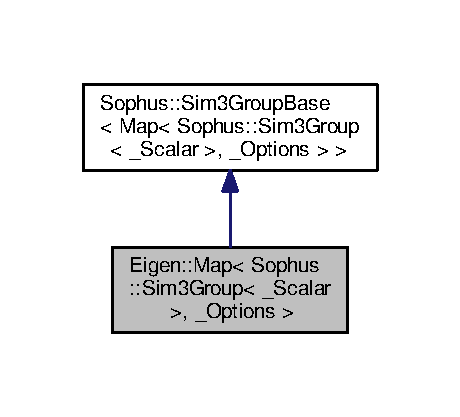
\includegraphics[width=221pt]{class_eigen_1_1_map_3_01_sophus_1_1_sim3_group_3_01___scalar_01_4_00_01___options_01_4__inherit__graph}
\end{center}
\end{figure}


Collaboration diagram for Eigen\+:\+:Map$<$ Sophus\+:\+:Sim3\+Group$<$ \+\_\+\+Scalar $>$, \+\_\+\+Options $>$\+:
\nopagebreak
\begin{figure}[H]
\begin{center}
\leavevmode
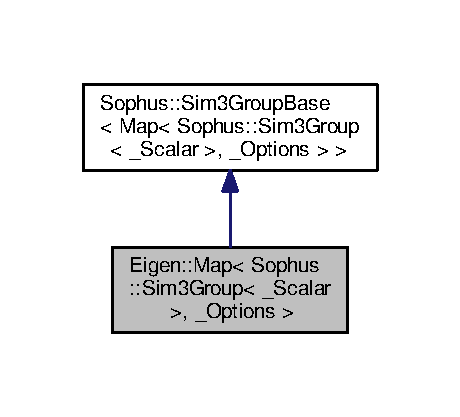
\includegraphics[width=221pt]{class_eigen_1_1_map_3_01_sophus_1_1_sim3_group_3_01___scalar_01_4_00_01___options_01_4__coll__graph}
\end{center}
\end{figure}
\subsection*{Public Types}
\begin{DoxyCompactItemize}
\item 
typedef internal\+::traits$<$ Map $>$\+::\hyperlink{class_eigen_1_1_map_3_01_sophus_1_1_sim3_group_3_01___scalar_01_4_00_01___options_01_4_a86a161ee4ef7691f50a6de409dda5a3e}{Scalar} \hyperlink{class_eigen_1_1_map_3_01_sophus_1_1_sim3_group_3_01___scalar_01_4_00_01___options_01_4_a86a161ee4ef7691f50a6de409dda5a3e}{Scalar}\hypertarget{class_eigen_1_1_map_3_01_sophus_1_1_sim3_group_3_01___scalar_01_4_00_01___options_01_4_a86a161ee4ef7691f50a6de409dda5a3e}{}\label{class_eigen_1_1_map_3_01_sophus_1_1_sim3_group_3_01___scalar_01_4_00_01___options_01_4_a86a161ee4ef7691f50a6de409dda5a3e}

\begin{DoxyCompactList}\small\item\em scalar type \end{DoxyCompactList}\item 
typedef internal\+::traits$<$ Map $>$\+::Translation\+Type \& \hyperlink{class_eigen_1_1_map_3_01_sophus_1_1_sim3_group_3_01___scalar_01_4_00_01___options_01_4_ac20dcaba9f5cca24de324bbd62cb6024}{Translation\+Reference}\hypertarget{class_eigen_1_1_map_3_01_sophus_1_1_sim3_group_3_01___scalar_01_4_00_01___options_01_4_ac20dcaba9f5cca24de324bbd62cb6024}{}\label{class_eigen_1_1_map_3_01_sophus_1_1_sim3_group_3_01___scalar_01_4_00_01___options_01_4_ac20dcaba9f5cca24de324bbd62cb6024}

\begin{DoxyCompactList}\small\item\em translation reference type \end{DoxyCompactList}\item 
typedef const internal\+::traits$<$ Map $>$\+::Translation\+Type \& \hyperlink{class_eigen_1_1_map_3_01_sophus_1_1_sim3_group_3_01___scalar_01_4_00_01___options_01_4_a922a4d47116d43b66cc711cbe71b2b29}{Const\+Translation\+Reference}\hypertarget{class_eigen_1_1_map_3_01_sophus_1_1_sim3_group_3_01___scalar_01_4_00_01___options_01_4_a922a4d47116d43b66cc711cbe71b2b29}{}\label{class_eigen_1_1_map_3_01_sophus_1_1_sim3_group_3_01___scalar_01_4_00_01___options_01_4_a922a4d47116d43b66cc711cbe71b2b29}

\begin{DoxyCompactList}\small\item\em translation const reference type \end{DoxyCompactList}\item 
typedef internal\+::traits$<$ Map $>$\+::Rx\+S\+O3\+Type \& \hyperlink{class_eigen_1_1_map_3_01_sophus_1_1_sim3_group_3_01___scalar_01_4_00_01___options_01_4_a1125dae9dde0a4f3394e10bd952808e1}{Rx\+S\+O3\+Reference}\hypertarget{class_eigen_1_1_map_3_01_sophus_1_1_sim3_group_3_01___scalar_01_4_00_01___options_01_4_a1125dae9dde0a4f3394e10bd952808e1}{}\label{class_eigen_1_1_map_3_01_sophus_1_1_sim3_group_3_01___scalar_01_4_00_01___options_01_4_a1125dae9dde0a4f3394e10bd952808e1}

\begin{DoxyCompactList}\small\item\em Rx\+S\+O3 reference type. \end{DoxyCompactList}\item 
typedef const internal\+::traits$<$ Map $>$\+::Rx\+S\+O3\+Type \& \hyperlink{class_eigen_1_1_map_3_01_sophus_1_1_sim3_group_3_01___scalar_01_4_00_01___options_01_4_a5b6f2c0d97bc193687b853f2e73c557a}{Const\+Rx\+S\+O3\+Reference}\hypertarget{class_eigen_1_1_map_3_01_sophus_1_1_sim3_group_3_01___scalar_01_4_00_01___options_01_4_a5b6f2c0d97bc193687b853f2e73c557a}{}\label{class_eigen_1_1_map_3_01_sophus_1_1_sim3_group_3_01___scalar_01_4_00_01___options_01_4_a5b6f2c0d97bc193687b853f2e73c557a}

\begin{DoxyCompactList}\small\item\em Rx\+S\+O3 const reference type. \end{DoxyCompactList}\item 
typedef \hyperlink{class_sophus_1_1_sim3_group_base_a93c8c564e3386709dc4cb2fc6d451dd8}{Base\+::\+Transformation} \hyperlink{class_eigen_1_1_map_3_01_sophus_1_1_sim3_group_3_01___scalar_01_4_00_01___options_01_4_ae5c102ed7c31df2b28d05f110decf0c1}{Transformation}\hypertarget{class_eigen_1_1_map_3_01_sophus_1_1_sim3_group_3_01___scalar_01_4_00_01___options_01_4_ae5c102ed7c31df2b28d05f110decf0c1}{}\label{class_eigen_1_1_map_3_01_sophus_1_1_sim3_group_3_01___scalar_01_4_00_01___options_01_4_ae5c102ed7c31df2b28d05f110decf0c1}

\begin{DoxyCompactList}\small\item\em group transfomation type \end{DoxyCompactList}\item 
typedef \hyperlink{class_sophus_1_1_sim3_group_base_a4b50c6b94e402746e50076305781dc9d}{Base\+::\+Point} \hyperlink{class_eigen_1_1_map_3_01_sophus_1_1_sim3_group_3_01___scalar_01_4_00_01___options_01_4_ab2164ab2258180c0a48da013cb8d7c05}{Point}\hypertarget{class_eigen_1_1_map_3_01_sophus_1_1_sim3_group_3_01___scalar_01_4_00_01___options_01_4_ab2164ab2258180c0a48da013cb8d7c05}{}\label{class_eigen_1_1_map_3_01_sophus_1_1_sim3_group_3_01___scalar_01_4_00_01___options_01_4_ab2164ab2258180c0a48da013cb8d7c05}

\begin{DoxyCompactList}\small\item\em point type \end{DoxyCompactList}\item 
typedef \hyperlink{class_sophus_1_1_sim3_group_base_a0f61582b6d8fa46ecbb40d70c87b632c}{Base\+::\+Tangent} \hyperlink{class_eigen_1_1_map_3_01_sophus_1_1_sim3_group_3_01___scalar_01_4_00_01___options_01_4_a26dec0e9d8bc51e5398437d6c02e5d6c}{Tangent}\hypertarget{class_eigen_1_1_map_3_01_sophus_1_1_sim3_group_3_01___scalar_01_4_00_01___options_01_4_a26dec0e9d8bc51e5398437d6c02e5d6c}{}\label{class_eigen_1_1_map_3_01_sophus_1_1_sim3_group_3_01___scalar_01_4_00_01___options_01_4_a26dec0e9d8bc51e5398437d6c02e5d6c}

\begin{DoxyCompactList}\small\item\em tangent vector type \end{DoxyCompactList}\item 
typedef \hyperlink{class_sophus_1_1_sim3_group_base_a7aa93f325ac7b811db77652f488e8f03}{Base\+::\+Adjoint} \hyperlink{class_eigen_1_1_map_3_01_sophus_1_1_sim3_group_3_01___scalar_01_4_00_01___options_01_4_aff53f7e3714d4655d559f076aafd0d20}{Adjoint}\hypertarget{class_eigen_1_1_map_3_01_sophus_1_1_sim3_group_3_01___scalar_01_4_00_01___options_01_4_aff53f7e3714d4655d559f076aafd0d20}{}\label{class_eigen_1_1_map_3_01_sophus_1_1_sim3_group_3_01___scalar_01_4_00_01___options_01_4_aff53f7e3714d4655d559f076aafd0d20}

\begin{DoxyCompactList}\small\item\em adjoint transformation type \end{DoxyCompactList}\end{DoxyCompactItemize}
\subsection*{Public Member Functions}
\begin{DoxyCompactItemize}
\item 
E\+I\+G\+E\+N\+\_\+\+S\+T\+R\+O\+N\+G\+\_\+\+I\+N\+L\+I\+NE {\bfseries Map} (\hyperlink{class_eigen_1_1_map_3_01_sophus_1_1_sim3_group_3_01___scalar_01_4_00_01___options_01_4_a86a161ee4ef7691f50a6de409dda5a3e}{Scalar} $\ast$coeffs)\hypertarget{class_eigen_1_1_map_3_01_sophus_1_1_sim3_group_3_01___scalar_01_4_00_01___options_01_4_ae2e87cbe54da01155ccfeda5d71ca9ee}{}\label{class_eigen_1_1_map_3_01_sophus_1_1_sim3_group_3_01___scalar_01_4_00_01___options_01_4_ae2e87cbe54da01155ccfeda5d71ca9ee}

\item 
E\+I\+G\+E\+N\+\_\+\+S\+T\+R\+O\+N\+G\+\_\+\+I\+N\+L\+I\+NE \hyperlink{class_eigen_1_1_map_3_01_sophus_1_1_sim3_group_3_01___scalar_01_4_00_01___options_01_4_a1125dae9dde0a4f3394e10bd952808e1}{Rx\+S\+O3\+Reference} \hyperlink{class_eigen_1_1_map_3_01_sophus_1_1_sim3_group_3_01___scalar_01_4_00_01___options_01_4_ae31b45e7edf7795b3e4097770c120f9f}{rxso3} ()\hypertarget{class_eigen_1_1_map_3_01_sophus_1_1_sim3_group_3_01___scalar_01_4_00_01___options_01_4_ae31b45e7edf7795b3e4097770c120f9f}{}\label{class_eigen_1_1_map_3_01_sophus_1_1_sim3_group_3_01___scalar_01_4_00_01___options_01_4_ae31b45e7edf7795b3e4097770c120f9f}

\begin{DoxyCompactList}\small\item\em Mutator of Rx\+S\+O3. \end{DoxyCompactList}\item 
E\+I\+G\+E\+N\+\_\+\+S\+T\+R\+O\+N\+G\+\_\+\+I\+N\+L\+I\+NE \hyperlink{class_eigen_1_1_map_3_01_sophus_1_1_sim3_group_3_01___scalar_01_4_00_01___options_01_4_a5b6f2c0d97bc193687b853f2e73c557a}{Const\+Rx\+S\+O3\+Reference} \hyperlink{class_eigen_1_1_map_3_01_sophus_1_1_sim3_group_3_01___scalar_01_4_00_01___options_01_4_a412fb76a0d495b3c940a9c84a5a14f89}{rxso3} () const \hypertarget{class_eigen_1_1_map_3_01_sophus_1_1_sim3_group_3_01___scalar_01_4_00_01___options_01_4_a412fb76a0d495b3c940a9c84a5a14f89}{}\label{class_eigen_1_1_map_3_01_sophus_1_1_sim3_group_3_01___scalar_01_4_00_01___options_01_4_a412fb76a0d495b3c940a9c84a5a14f89}

\begin{DoxyCompactList}\small\item\em Accessor of Rx\+S\+O3. \end{DoxyCompactList}\item 
E\+I\+G\+E\+N\+\_\+\+S\+T\+R\+O\+N\+G\+\_\+\+I\+N\+L\+I\+NE \hyperlink{class_eigen_1_1_map_3_01_sophus_1_1_sim3_group_3_01___scalar_01_4_00_01___options_01_4_ac20dcaba9f5cca24de324bbd62cb6024}{Translation\+Reference} \hyperlink{class_eigen_1_1_map_3_01_sophus_1_1_sim3_group_3_01___scalar_01_4_00_01___options_01_4_a5c3730af1c036d3dd13b8158fb0a10fa}{translation} ()\hypertarget{class_eigen_1_1_map_3_01_sophus_1_1_sim3_group_3_01___scalar_01_4_00_01___options_01_4_a5c3730af1c036d3dd13b8158fb0a10fa}{}\label{class_eigen_1_1_map_3_01_sophus_1_1_sim3_group_3_01___scalar_01_4_00_01___options_01_4_a5c3730af1c036d3dd13b8158fb0a10fa}

\begin{DoxyCompactList}\small\item\em Mutator of translation vector. \end{DoxyCompactList}\item 
E\+I\+G\+E\+N\+\_\+\+S\+T\+R\+O\+N\+G\+\_\+\+I\+N\+L\+I\+NE \hyperlink{class_eigen_1_1_map_3_01_sophus_1_1_sim3_group_3_01___scalar_01_4_00_01___options_01_4_a922a4d47116d43b66cc711cbe71b2b29}{Const\+Translation\+Reference} \hyperlink{class_eigen_1_1_map_3_01_sophus_1_1_sim3_group_3_01___scalar_01_4_00_01___options_01_4_a076e842c0bdc2ee23efd660bb53720d6}{translation} () const \hypertarget{class_eigen_1_1_map_3_01_sophus_1_1_sim3_group_3_01___scalar_01_4_00_01___options_01_4_a076e842c0bdc2ee23efd660bb53720d6}{}\label{class_eigen_1_1_map_3_01_sophus_1_1_sim3_group_3_01___scalar_01_4_00_01___options_01_4_a076e842c0bdc2ee23efd660bb53720d6}

\begin{DoxyCompactList}\small\item\em Accessor of translation vector. \end{DoxyCompactList}\end{DoxyCompactItemize}
\subsection*{Static Public Attributes}
\begin{DoxyCompactItemize}
\item 
static const int \hyperlink{class_eigen_1_1_map_3_01_sophus_1_1_sim3_group_3_01___scalar_01_4_00_01___options_01_4_acbea93953d7630022c328a3a974422d8}{DoF} = Base\+::\+DoF\hypertarget{class_eigen_1_1_map_3_01_sophus_1_1_sim3_group_3_01___scalar_01_4_00_01___options_01_4_acbea93953d7630022c328a3a974422d8}{}\label{class_eigen_1_1_map_3_01_sophus_1_1_sim3_group_3_01___scalar_01_4_00_01___options_01_4_acbea93953d7630022c328a3a974422d8}

\begin{DoxyCompactList}\small\item\em degree of freedom of group \end{DoxyCompactList}\item 
static const int \hyperlink{class_eigen_1_1_map_3_01_sophus_1_1_sim3_group_3_01___scalar_01_4_00_01___options_01_4_a3af1d812541af8ccdf105d78b99c0590}{num\+\_\+parameters} = Base\+::num\+\_\+parameters\hypertarget{class_eigen_1_1_map_3_01_sophus_1_1_sim3_group_3_01___scalar_01_4_00_01___options_01_4_a3af1d812541af8ccdf105d78b99c0590}{}\label{class_eigen_1_1_map_3_01_sophus_1_1_sim3_group_3_01___scalar_01_4_00_01___options_01_4_a3af1d812541af8ccdf105d78b99c0590}

\begin{DoxyCompactList}\small\item\em number of internal parameters used \end{DoxyCompactList}\item 
static const int \hyperlink{class_eigen_1_1_map_3_01_sophus_1_1_sim3_group_3_01___scalar_01_4_00_01___options_01_4_a2574f0a81a3968ef5461686bb1c2d6e4}{N} = Base\+::N\hypertarget{class_eigen_1_1_map_3_01_sophus_1_1_sim3_group_3_01___scalar_01_4_00_01___options_01_4_a2574f0a81a3968ef5461686bb1c2d6e4}{}\label{class_eigen_1_1_map_3_01_sophus_1_1_sim3_group_3_01___scalar_01_4_00_01___options_01_4_a2574f0a81a3968ef5461686bb1c2d6e4}

\begin{DoxyCompactList}\small\item\em group transformations are NxN matrices \end{DoxyCompactList}\end{DoxyCompactItemize}
\subsection*{Protected Attributes}
\begin{DoxyCompactItemize}
\item 
Map$<$ \hyperlink{class_sophus_1_1_rx_s_o3_group}{Sophus\+::\+Rx\+S\+O3\+Group}$<$ \hyperlink{class_eigen_1_1_map_3_01_sophus_1_1_sim3_group_3_01___scalar_01_4_00_01___options_01_4_a86a161ee4ef7691f50a6de409dda5a3e}{Scalar} $>$, \+\_\+\+Options $>$ {\bfseries rxso3\+\_\+}\hypertarget{class_eigen_1_1_map_3_01_sophus_1_1_sim3_group_3_01___scalar_01_4_00_01___options_01_4_aaf4c1d4c7fb13868556c6620a7ef3c64}{}\label{class_eigen_1_1_map_3_01_sophus_1_1_sim3_group_3_01___scalar_01_4_00_01___options_01_4_aaf4c1d4c7fb13868556c6620a7ef3c64}

\item 
Map$<$ Matrix$<$ \hyperlink{class_eigen_1_1_map_3_01_sophus_1_1_sim3_group_3_01___scalar_01_4_00_01___options_01_4_a86a161ee4ef7691f50a6de409dda5a3e}{Scalar}, 3, 1 $>$, \+\_\+\+Options $>$ {\bfseries translation\+\_\+}\hypertarget{class_eigen_1_1_map_3_01_sophus_1_1_sim3_group_3_01___scalar_01_4_00_01___options_01_4_ad6bee375a3a2f9f7c05c7cd91bc81d7d}{}\label{class_eigen_1_1_map_3_01_sophus_1_1_sim3_group_3_01___scalar_01_4_00_01___options_01_4_ad6bee375a3a2f9f7c05c7cd91bc81d7d}

\end{DoxyCompactItemize}
\subsection*{Additional Inherited Members}


\subsection{Detailed Description}
\subsubsection*{template$<$typename \+\_\+\+Scalar, int \+\_\+\+Options$>$\\*
class Eigen\+::\+Map$<$ Sophus\+::\+Sim3\+Group$<$ \+\_\+\+Scalar $>$, \+\_\+\+Options $>$}

Specialisation of Eigen\+::\+Map for Sim3\+Group\+Base. 

Allows us to wrap Sim3 Objects around P\+OD array (e.\+g. external c style quaternion) 

Definition at line 816 of file sim3.\+hpp.



The documentation for this class was generated from the following file\+:\begin{DoxyCompactItemize}
\item 
include/\+Sophus/sophus/sim3.\+hpp\end{DoxyCompactItemize}

\hypertarget{class_eigen_1_1_map_3_01_sophus_1_1_s_o2_group_3_01___scalar_01_4_00_01___options_01_4}{}\section{Eigen\+:\+:Map$<$ Sophus\+:\+:S\+O2\+Group$<$ \+\_\+\+Scalar $>$, \+\_\+\+Options $>$ Class Template Reference}
\label{class_eigen_1_1_map_3_01_sophus_1_1_s_o2_group_3_01___scalar_01_4_00_01___options_01_4}\index{Eigen\+::\+Map$<$ Sophus\+::\+S\+O2\+Group$<$ \+\_\+\+Scalar $>$, \+\_\+\+Options $>$@{Eigen\+::\+Map$<$ Sophus\+::\+S\+O2\+Group$<$ \+\_\+\+Scalar $>$, \+\_\+\+Options $>$}}


Specialisation of Eigen\+::\+Map for S\+O2\+Group\+Base.  




{\ttfamily \#include $<$so2.\+hpp$>$}



Inheritance diagram for Eigen\+:\+:Map$<$ Sophus\+:\+:S\+O2\+Group$<$ \+\_\+\+Scalar $>$, \+\_\+\+Options $>$\+:
\nopagebreak
\begin{figure}[H]
\begin{center}
\leavevmode
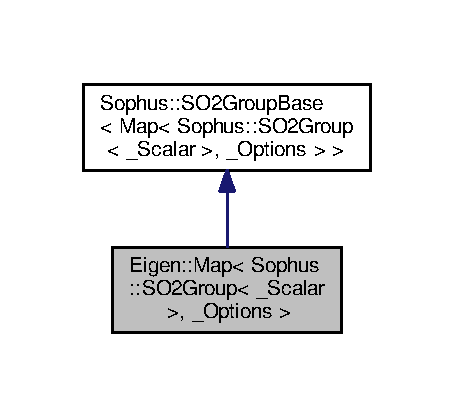
\includegraphics[width=218pt]{class_eigen_1_1_map_3_01_sophus_1_1_s_o2_group_3_01___scalar_01_4_00_01___options_01_4__inherit__graph}
\end{center}
\end{figure}


Collaboration diagram for Eigen\+:\+:Map$<$ Sophus\+:\+:S\+O2\+Group$<$ \+\_\+\+Scalar $>$, \+\_\+\+Options $>$\+:
\nopagebreak
\begin{figure}[H]
\begin{center}
\leavevmode
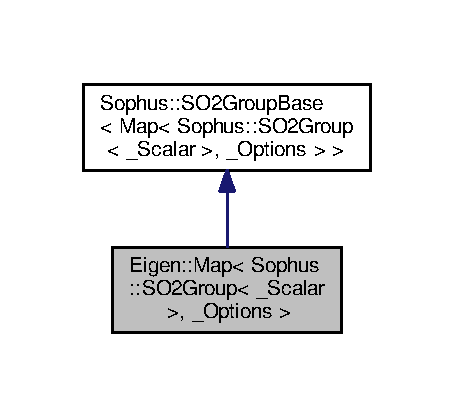
\includegraphics[width=218pt]{class_eigen_1_1_map_3_01_sophus_1_1_s_o2_group_3_01___scalar_01_4_00_01___options_01_4__coll__graph}
\end{center}
\end{figure}
\subsection*{Public Types}
\begin{DoxyCompactItemize}
\item 
typedef internal\+::traits$<$ Map $>$\+::\hyperlink{class_sophus_1_1_s_o2_group_base_a075b701502715aecf0bdb3464963d36c}{Scalar} \hyperlink{class_eigen_1_1_map_3_01_sophus_1_1_s_o2_group_3_01___scalar_01_4_00_01___options_01_4_ae6b0bc4f4e453419df11bcc15bf88ed8}{Scalar}\hypertarget{class_eigen_1_1_map_3_01_sophus_1_1_s_o2_group_3_01___scalar_01_4_00_01___options_01_4_ae6b0bc4f4e453419df11bcc15bf88ed8}{}\label{class_eigen_1_1_map_3_01_sophus_1_1_s_o2_group_3_01___scalar_01_4_00_01___options_01_4_ae6b0bc4f4e453419df11bcc15bf88ed8}

\begin{DoxyCompactList}\small\item\em scalar type \end{DoxyCompactList}\item 
typedef internal\+::traits$<$ Map $>$\+::Complex\+Type \& \hyperlink{class_eigen_1_1_map_3_01_sophus_1_1_s_o2_group_3_01___scalar_01_4_00_01___options_01_4_ac0a405be5117be77329dbc1498a1000c}{Complex\+Reference}\hypertarget{class_eigen_1_1_map_3_01_sophus_1_1_s_o2_group_3_01___scalar_01_4_00_01___options_01_4_ac0a405be5117be77329dbc1498a1000c}{}\label{class_eigen_1_1_map_3_01_sophus_1_1_s_o2_group_3_01___scalar_01_4_00_01___options_01_4_ac0a405be5117be77329dbc1498a1000c}

\begin{DoxyCompactList}\small\item\em complex number reference type \end{DoxyCompactList}\item 
typedef const internal\+::traits$<$ Map $>$\+::Complex\+Type \& \hyperlink{class_eigen_1_1_map_3_01_sophus_1_1_s_o2_group_3_01___scalar_01_4_00_01___options_01_4_a403f27ed222fae083641a79d9c4629c0}{Const\+Complex\+Reference}\hypertarget{class_eigen_1_1_map_3_01_sophus_1_1_s_o2_group_3_01___scalar_01_4_00_01___options_01_4_a403f27ed222fae083641a79d9c4629c0}{}\label{class_eigen_1_1_map_3_01_sophus_1_1_s_o2_group_3_01___scalar_01_4_00_01___options_01_4_a403f27ed222fae083641a79d9c4629c0}

\begin{DoxyCompactList}\small\item\em complex number const reference type \end{DoxyCompactList}\item 
typedef \hyperlink{class_sophus_1_1_s_o2_group_base_a8981dccaf65802191e989815046b6a82}{Base\+::\+Transformation} \hyperlink{class_eigen_1_1_map_3_01_sophus_1_1_s_o2_group_3_01___scalar_01_4_00_01___options_01_4_ad04ccbc06289dabfca623828588c55d8}{Transformation}\hypertarget{class_eigen_1_1_map_3_01_sophus_1_1_s_o2_group_3_01___scalar_01_4_00_01___options_01_4_ad04ccbc06289dabfca623828588c55d8}{}\label{class_eigen_1_1_map_3_01_sophus_1_1_s_o2_group_3_01___scalar_01_4_00_01___options_01_4_ad04ccbc06289dabfca623828588c55d8}

\begin{DoxyCompactList}\small\item\em group transfomation type \end{DoxyCompactList}\item 
typedef \hyperlink{class_sophus_1_1_s_o2_group_base_acdbb4a45d5f3d826b6bf8462c92c7f54}{Base\+::\+Point} \hyperlink{class_eigen_1_1_map_3_01_sophus_1_1_s_o2_group_3_01___scalar_01_4_00_01___options_01_4_a1f48433957fb63625e7b5d4f3e534b90}{Point}\hypertarget{class_eigen_1_1_map_3_01_sophus_1_1_s_o2_group_3_01___scalar_01_4_00_01___options_01_4_a1f48433957fb63625e7b5d4f3e534b90}{}\label{class_eigen_1_1_map_3_01_sophus_1_1_s_o2_group_3_01___scalar_01_4_00_01___options_01_4_a1f48433957fb63625e7b5d4f3e534b90}

\begin{DoxyCompactList}\small\item\em point type \end{DoxyCompactList}\item 
typedef \hyperlink{class_sophus_1_1_s_o2_group_base_a3701d07bf2791675518a0ceb33ce653b}{Base\+::\+Tangent} \hyperlink{class_eigen_1_1_map_3_01_sophus_1_1_s_o2_group_3_01___scalar_01_4_00_01___options_01_4_a091c581b154445b71d48300ea784c575}{Tangent}\hypertarget{class_eigen_1_1_map_3_01_sophus_1_1_s_o2_group_3_01___scalar_01_4_00_01___options_01_4_a091c581b154445b71d48300ea784c575}{}\label{class_eigen_1_1_map_3_01_sophus_1_1_s_o2_group_3_01___scalar_01_4_00_01___options_01_4_a091c581b154445b71d48300ea784c575}

\begin{DoxyCompactList}\small\item\em tangent vector type \end{DoxyCompactList}\item 
typedef \hyperlink{class_sophus_1_1_s_o2_group_base_a02b4843e52df827cf466eacd288697fa}{Base\+::\+Adjoint} \hyperlink{class_eigen_1_1_map_3_01_sophus_1_1_s_o2_group_3_01___scalar_01_4_00_01___options_01_4_aec8f621c2f2c765107717d456707eccb}{Adjoint}\hypertarget{class_eigen_1_1_map_3_01_sophus_1_1_s_o2_group_3_01___scalar_01_4_00_01___options_01_4_aec8f621c2f2c765107717d456707eccb}{}\label{class_eigen_1_1_map_3_01_sophus_1_1_s_o2_group_3_01___scalar_01_4_00_01___options_01_4_aec8f621c2f2c765107717d456707eccb}

\begin{DoxyCompactList}\small\item\em adjoint transformation type \end{DoxyCompactList}\end{DoxyCompactItemize}
\subsection*{Public Member Functions}
\begin{DoxyCompactItemize}
\item 
E\+I\+G\+E\+N\+\_\+\+S\+T\+R\+O\+N\+G\+\_\+\+I\+N\+L\+I\+NE {\bfseries Map} (\hyperlink{class_sophus_1_1_s_o2_group_base_a075b701502715aecf0bdb3464963d36c}{Scalar} $\ast$coeffs)\hypertarget{class_eigen_1_1_map_3_01_sophus_1_1_s_o2_group_3_01___scalar_01_4_00_01___options_01_4_a8d91e157d048d775c835066cd8ebbc3c}{}\label{class_eigen_1_1_map_3_01_sophus_1_1_s_o2_group_3_01___scalar_01_4_00_01___options_01_4_a8d91e157d048d775c835066cd8ebbc3c}

\item 
E\+I\+G\+E\+N\+\_\+\+S\+T\+R\+O\+N\+G\+\_\+\+I\+N\+L\+I\+NE \hyperlink{class_sophus_1_1_s_o2_group_base_a077856f95a5c02933efd03aa1393825f}{Const\+Complex\+Reference} \hyperlink{class_eigen_1_1_map_3_01_sophus_1_1_s_o2_group_3_01___scalar_01_4_00_01___options_01_4_af4497aa46d2216a58be7e674109c8b30}{unit\+\_\+complex} () const 
\begin{DoxyCompactList}\small\item\em Accessor of unit complex number. \end{DoxyCompactList}\end{DoxyCompactItemize}
\subsection*{Static Public Attributes}
\begin{DoxyCompactItemize}
\item 
static const int \hyperlink{class_eigen_1_1_map_3_01_sophus_1_1_s_o2_group_3_01___scalar_01_4_00_01___options_01_4_aca2d5e70b128b11ad03cf07452827fc0}{DoF} = Base\+::\+DoF\hypertarget{class_eigen_1_1_map_3_01_sophus_1_1_s_o2_group_3_01___scalar_01_4_00_01___options_01_4_aca2d5e70b128b11ad03cf07452827fc0}{}\label{class_eigen_1_1_map_3_01_sophus_1_1_s_o2_group_3_01___scalar_01_4_00_01___options_01_4_aca2d5e70b128b11ad03cf07452827fc0}

\begin{DoxyCompactList}\small\item\em degree of freedom of group \end{DoxyCompactList}\item 
static const int \hyperlink{class_eigen_1_1_map_3_01_sophus_1_1_s_o2_group_3_01___scalar_01_4_00_01___options_01_4_aa0dc4364c71cc0dc34f47b1f2442fc38}{num\+\_\+parameters} = Base\+::num\+\_\+parameters\hypertarget{class_eigen_1_1_map_3_01_sophus_1_1_s_o2_group_3_01___scalar_01_4_00_01___options_01_4_aa0dc4364c71cc0dc34f47b1f2442fc38}{}\label{class_eigen_1_1_map_3_01_sophus_1_1_s_o2_group_3_01___scalar_01_4_00_01___options_01_4_aa0dc4364c71cc0dc34f47b1f2442fc38}

\begin{DoxyCompactList}\small\item\em number of internal parameters used \end{DoxyCompactList}\item 
static const int \hyperlink{class_eigen_1_1_map_3_01_sophus_1_1_s_o2_group_3_01___scalar_01_4_00_01___options_01_4_a49b4012e6e4d2cca28682a304d41ab0e}{N} = Base\+::N\hypertarget{class_eigen_1_1_map_3_01_sophus_1_1_s_o2_group_3_01___scalar_01_4_00_01___options_01_4_a49b4012e6e4d2cca28682a304d41ab0e}{}\label{class_eigen_1_1_map_3_01_sophus_1_1_s_o2_group_3_01___scalar_01_4_00_01___options_01_4_a49b4012e6e4d2cca28682a304d41ab0e}

\begin{DoxyCompactList}\small\item\em group transformations are NxN matrices \end{DoxyCompactList}\end{DoxyCompactItemize}
\subsection*{Protected Member Functions}
\begin{DoxyCompactItemize}
\item 
E\+I\+G\+E\+N\+\_\+\+S\+T\+R\+O\+N\+G\+\_\+\+I\+N\+L\+I\+NE \hyperlink{class_sophus_1_1_s_o2_group_base_adad5730f4c0387415b8dfc3c5aa8b8f2}{Complex\+Reference} {\bfseries unit\+\_\+complex\+\_\+nonconst} ()\hypertarget{class_eigen_1_1_map_3_01_sophus_1_1_s_o2_group_3_01___scalar_01_4_00_01___options_01_4_ad637c564d4e231a16f971791309ed864}{}\label{class_eigen_1_1_map_3_01_sophus_1_1_s_o2_group_3_01___scalar_01_4_00_01___options_01_4_ad637c564d4e231a16f971791309ed864}

\end{DoxyCompactItemize}
\subsection*{Protected Attributes}
\begin{DoxyCompactItemize}
\item 
Map$<$ Matrix$<$ \hyperlink{class_sophus_1_1_s_o2_group_base_a075b701502715aecf0bdb3464963d36c}{Scalar}, 2, 1 $>$, \+\_\+\+Options $>$ {\bfseries unit\+\_\+complex\+\_\+}\hypertarget{class_eigen_1_1_map_3_01_sophus_1_1_s_o2_group_3_01___scalar_01_4_00_01___options_01_4_a2318aec787c38165fb7fecfbcd3a7351}{}\label{class_eigen_1_1_map_3_01_sophus_1_1_s_o2_group_3_01___scalar_01_4_00_01___options_01_4_a2318aec787c38165fb7fecfbcd3a7351}

\end{DoxyCompactItemize}
\subsection*{Friends}
\begin{DoxyCompactItemize}
\item 
class {\bfseries Sophus\+::\+S\+O2\+Group\+Base$<$ Map$<$ Sophus\+::\+S\+O2\+Group$<$ \+\_\+\+Scalar $>$, \+\_\+\+Options $>$ $>$}\hypertarget{class_eigen_1_1_map_3_01_sophus_1_1_s_o2_group_3_01___scalar_01_4_00_01___options_01_4_aea5acf253f378df2d3e992e737e6245f}{}\label{class_eigen_1_1_map_3_01_sophus_1_1_s_o2_group_3_01___scalar_01_4_00_01___options_01_4_aea5acf253f378df2d3e992e737e6245f}

\end{DoxyCompactItemize}
\subsection*{Additional Inherited Members}


\subsection{Detailed Description}
\subsubsection*{template$<$typename \+\_\+\+Scalar, int \+\_\+\+Options$>$\\*
class Eigen\+::\+Map$<$ Sophus\+::\+S\+O2\+Group$<$ \+\_\+\+Scalar $>$, \+\_\+\+Options $>$}

Specialisation of Eigen\+::\+Map for S\+O2\+Group\+Base. 

Allows us to wrap S\+O2 Objects around P\+OD array (e.\+g. external c style complex number) 

Definition at line 578 of file so2.\+hpp.



\subsection{Member Function Documentation}
\index{Eigen\+::\+Map$<$ Sophus\+::\+S\+O2\+Group$<$ \+\_\+\+Scalar $>$, \+\_\+\+Options $>$@{Eigen\+::\+Map$<$ Sophus\+::\+S\+O2\+Group$<$ \+\_\+\+Scalar $>$, \+\_\+\+Options $>$}!unit\+\_\+complex@{unit\+\_\+complex}}
\index{unit\+\_\+complex@{unit\+\_\+complex}!Eigen\+::\+Map$<$ Sophus\+::\+S\+O2\+Group$<$ \+\_\+\+Scalar $>$, \+\_\+\+Options $>$@{Eigen\+::\+Map$<$ Sophus\+::\+S\+O2\+Group$<$ \+\_\+\+Scalar $>$, \+\_\+\+Options $>$}}
\subsubsection[{\texorpdfstring{unit\+\_\+complex() const }{unit_complex() const }}]{\setlength{\rightskip}{0pt plus 5cm}template$<$typename \+\_\+\+Scalar , int \+\_\+\+Options$>$ E\+I\+G\+E\+N\+\_\+\+S\+T\+R\+O\+N\+G\+\_\+\+I\+N\+L\+I\+NE {\bf Const\+Complex\+Reference} Eigen\+::\+Map$<$ {\bf Sophus\+::\+S\+O2\+Group}$<$ \+\_\+\+Scalar $>$, \+\_\+\+Options $>$\+::unit\+\_\+complex (
\begin{DoxyParamCaption}
{}
\end{DoxyParamCaption}
) const\hspace{0.3cm}{\ttfamily [inline]}}\hypertarget{class_eigen_1_1_map_3_01_sophus_1_1_s_o2_group_3_01___scalar_01_4_00_01___options_01_4_af4497aa46d2216a58be7e674109c8b30}{}\label{class_eigen_1_1_map_3_01_sophus_1_1_s_o2_group_3_01___scalar_01_4_00_01___options_01_4_af4497aa46d2216a58be7e674109c8b30}


Accessor of unit complex number. 

No direct write access is given to ensure the complex number stays normalized. 

Definition at line 624 of file so2.\+hpp.



The documentation for this class was generated from the following file\+:\begin{DoxyCompactItemize}
\item 
include/\+Sophus/sophus/so2.\+hpp\end{DoxyCompactItemize}

\hypertarget{class_eigen_1_1_map_3_01_sophus_1_1_s_o3_group_3_01___scalar_01_4_00_01___options_01_4}{}\section{Eigen\+:\+:Map$<$ Sophus\+:\+:S\+O3\+Group$<$ \+\_\+\+Scalar $>$, \+\_\+\+Options $>$ Class Template Reference}
\label{class_eigen_1_1_map_3_01_sophus_1_1_s_o3_group_3_01___scalar_01_4_00_01___options_01_4}\index{Eigen\+::\+Map$<$ Sophus\+::\+S\+O3\+Group$<$ \+\_\+\+Scalar $>$, \+\_\+\+Options $>$@{Eigen\+::\+Map$<$ Sophus\+::\+S\+O3\+Group$<$ \+\_\+\+Scalar $>$, \+\_\+\+Options $>$}}


Specialisation of Eigen\+::\+Map for S\+O3\+Group\+Base.  




{\ttfamily \#include $<$so3.\+hpp$>$}



Inheritance diagram for Eigen\+:\+:Map$<$ Sophus\+:\+:S\+O3\+Group$<$ \+\_\+\+Scalar $>$, \+\_\+\+Options $>$\+:
\nopagebreak
\begin{figure}[H]
\begin{center}
\leavevmode
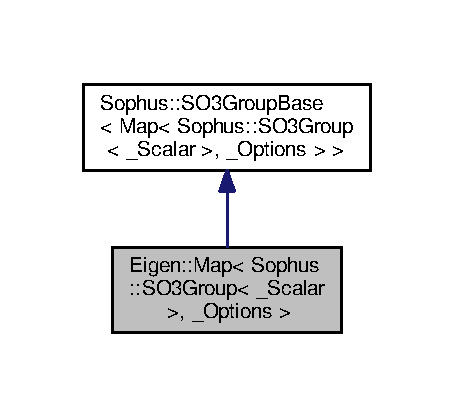
\includegraphics[width=218pt]{class_eigen_1_1_map_3_01_sophus_1_1_s_o3_group_3_01___scalar_01_4_00_01___options_01_4__inherit__graph}
\end{center}
\end{figure}


Collaboration diagram for Eigen\+:\+:Map$<$ Sophus\+:\+:S\+O3\+Group$<$ \+\_\+\+Scalar $>$, \+\_\+\+Options $>$\+:
\nopagebreak
\begin{figure}[H]
\begin{center}
\leavevmode
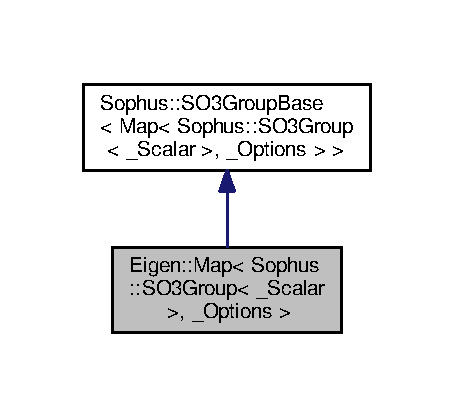
\includegraphics[width=218pt]{class_eigen_1_1_map_3_01_sophus_1_1_s_o3_group_3_01___scalar_01_4_00_01___options_01_4__coll__graph}
\end{center}
\end{figure}
\subsection*{Public Types}
\begin{DoxyCompactItemize}
\item 
typedef internal\+::traits$<$ Map $>$\+::\hyperlink{class_sophus_1_1_s_o3_group_base_a31bf31815c195b7150da8a8e8c6f0189}{Scalar} \hyperlink{class_eigen_1_1_map_3_01_sophus_1_1_s_o3_group_3_01___scalar_01_4_00_01___options_01_4_a3847af0a5bb7bf1ae0d47c57b7aed2a5}{Scalar}\hypertarget{class_eigen_1_1_map_3_01_sophus_1_1_s_o3_group_3_01___scalar_01_4_00_01___options_01_4_a3847af0a5bb7bf1ae0d47c57b7aed2a5}{}\label{class_eigen_1_1_map_3_01_sophus_1_1_s_o3_group_3_01___scalar_01_4_00_01___options_01_4_a3847af0a5bb7bf1ae0d47c57b7aed2a5}

\begin{DoxyCompactList}\small\item\em scalar type \end{DoxyCompactList}\item 
typedef internal\+::traits$<$ Map $>$\+::Quaternion\+Type \& \hyperlink{class_eigen_1_1_map_3_01_sophus_1_1_s_o3_group_3_01___scalar_01_4_00_01___options_01_4_a86c67489696ba95023fc4c6ad5c616ef}{Quaternion\+Reference}\hypertarget{class_eigen_1_1_map_3_01_sophus_1_1_s_o3_group_3_01___scalar_01_4_00_01___options_01_4_a86c67489696ba95023fc4c6ad5c616ef}{}\label{class_eigen_1_1_map_3_01_sophus_1_1_s_o3_group_3_01___scalar_01_4_00_01___options_01_4_a86c67489696ba95023fc4c6ad5c616ef}

\begin{DoxyCompactList}\small\item\em quaternion reference type \end{DoxyCompactList}\item 
typedef const internal\+::traits$<$ Map $>$\+::Quaternion\+Type \& \hyperlink{class_eigen_1_1_map_3_01_sophus_1_1_s_o3_group_3_01___scalar_01_4_00_01___options_01_4_a164920d3a48953a81c8c0544bdeed46c}{Const\+Quaternion\+Reference}\hypertarget{class_eigen_1_1_map_3_01_sophus_1_1_s_o3_group_3_01___scalar_01_4_00_01___options_01_4_a164920d3a48953a81c8c0544bdeed46c}{}\label{class_eigen_1_1_map_3_01_sophus_1_1_s_o3_group_3_01___scalar_01_4_00_01___options_01_4_a164920d3a48953a81c8c0544bdeed46c}

\begin{DoxyCompactList}\small\item\em quaternion const reference type \end{DoxyCompactList}\item 
typedef \hyperlink{class_sophus_1_1_s_o3_group_base_aa20fc57bf1b355a6616f5c4b785f1fc5}{Base\+::\+Transformation} \hyperlink{class_eigen_1_1_map_3_01_sophus_1_1_s_o3_group_3_01___scalar_01_4_00_01___options_01_4_a34a03facbc8491b9ac83081eea2b369f}{Transformation}\hypertarget{class_eigen_1_1_map_3_01_sophus_1_1_s_o3_group_3_01___scalar_01_4_00_01___options_01_4_a34a03facbc8491b9ac83081eea2b369f}{}\label{class_eigen_1_1_map_3_01_sophus_1_1_s_o3_group_3_01___scalar_01_4_00_01___options_01_4_a34a03facbc8491b9ac83081eea2b369f}

\begin{DoxyCompactList}\small\item\em group transfomation type \end{DoxyCompactList}\item 
typedef \hyperlink{class_sophus_1_1_s_o3_group_base_a1cfbc3b3a28e1f70b3e1845716db0a1b}{Base\+::\+Point} \hyperlink{class_eigen_1_1_map_3_01_sophus_1_1_s_o3_group_3_01___scalar_01_4_00_01___options_01_4_aa8eab29f0854cdcfcb63afdb8a43661f}{Point}\hypertarget{class_eigen_1_1_map_3_01_sophus_1_1_s_o3_group_3_01___scalar_01_4_00_01___options_01_4_aa8eab29f0854cdcfcb63afdb8a43661f}{}\label{class_eigen_1_1_map_3_01_sophus_1_1_s_o3_group_3_01___scalar_01_4_00_01___options_01_4_aa8eab29f0854cdcfcb63afdb8a43661f}

\begin{DoxyCompactList}\small\item\em point type \end{DoxyCompactList}\item 
typedef \hyperlink{class_sophus_1_1_s_o3_group_base_a11150229b6a471ae96cde974ece5ec7c}{Base\+::\+Tangent} \hyperlink{class_eigen_1_1_map_3_01_sophus_1_1_s_o3_group_3_01___scalar_01_4_00_01___options_01_4_a44cf260ef409fd6f1af38dcdec25ffb4}{Tangent}\hypertarget{class_eigen_1_1_map_3_01_sophus_1_1_s_o3_group_3_01___scalar_01_4_00_01___options_01_4_a44cf260ef409fd6f1af38dcdec25ffb4}{}\label{class_eigen_1_1_map_3_01_sophus_1_1_s_o3_group_3_01___scalar_01_4_00_01___options_01_4_a44cf260ef409fd6f1af38dcdec25ffb4}

\begin{DoxyCompactList}\small\item\em tangent vector type \end{DoxyCompactList}\item 
typedef \hyperlink{class_sophus_1_1_s_o3_group_base_a51c46f75563c21fbd223b4a444923306}{Base\+::\+Adjoint} \hyperlink{class_eigen_1_1_map_3_01_sophus_1_1_s_o3_group_3_01___scalar_01_4_00_01___options_01_4_a69a485b4b0a819e22ebd5c78ce65c7f8}{Adjoint}\hypertarget{class_eigen_1_1_map_3_01_sophus_1_1_s_o3_group_3_01___scalar_01_4_00_01___options_01_4_a69a485b4b0a819e22ebd5c78ce65c7f8}{}\label{class_eigen_1_1_map_3_01_sophus_1_1_s_o3_group_3_01___scalar_01_4_00_01___options_01_4_a69a485b4b0a819e22ebd5c78ce65c7f8}

\begin{DoxyCompactList}\small\item\em adjoint transformation type \end{DoxyCompactList}\end{DoxyCompactItemize}
\subsection*{Public Member Functions}
\begin{DoxyCompactItemize}
\item 
E\+I\+G\+E\+N\+\_\+\+S\+T\+R\+O\+N\+G\+\_\+\+I\+N\+L\+I\+NE {\bfseries Map} (\hyperlink{class_sophus_1_1_s_o3_group_base_a31bf31815c195b7150da8a8e8c6f0189}{Scalar} $\ast$coeffs)\hypertarget{class_eigen_1_1_map_3_01_sophus_1_1_s_o3_group_3_01___scalar_01_4_00_01___options_01_4_a13c62e8dbdb994debb0ce6a7931a3a15}{}\label{class_eigen_1_1_map_3_01_sophus_1_1_s_o3_group_3_01___scalar_01_4_00_01___options_01_4_a13c62e8dbdb994debb0ce6a7931a3a15}

\item 
E\+I\+G\+E\+N\+\_\+\+S\+T\+R\+O\+N\+G\+\_\+\+I\+N\+L\+I\+NE \hyperlink{class_sophus_1_1_s_o3_group_base_a8a5a23aee10f2850a5894b7c1f5e6654}{Const\+Quaternion\+Reference} \hyperlink{class_eigen_1_1_map_3_01_sophus_1_1_s_o3_group_3_01___scalar_01_4_00_01___options_01_4_ae35daf5e45b340c471fac3f3d2b03c4d}{unit\+\_\+quaternion} () const 
\begin{DoxyCompactList}\small\item\em Accessor of unit quaternion. \end{DoxyCompactList}\end{DoxyCompactItemize}
\subsection*{Static Public Attributes}
\begin{DoxyCompactItemize}
\item 
static const int \hyperlink{class_eigen_1_1_map_3_01_sophus_1_1_s_o3_group_3_01___scalar_01_4_00_01___options_01_4_a07f8eea132e935274ff3c262a1abd073}{DoF} = Base\+::\+DoF\hypertarget{class_eigen_1_1_map_3_01_sophus_1_1_s_o3_group_3_01___scalar_01_4_00_01___options_01_4_a07f8eea132e935274ff3c262a1abd073}{}\label{class_eigen_1_1_map_3_01_sophus_1_1_s_o3_group_3_01___scalar_01_4_00_01___options_01_4_a07f8eea132e935274ff3c262a1abd073}

\begin{DoxyCompactList}\small\item\em degree of freedom of group \end{DoxyCompactList}\item 
static const int \hyperlink{class_eigen_1_1_map_3_01_sophus_1_1_s_o3_group_3_01___scalar_01_4_00_01___options_01_4_aec066d5fe30169cf4eb5d5adde1f8e5c}{num\+\_\+parameters} = Base\+::num\+\_\+parameters\hypertarget{class_eigen_1_1_map_3_01_sophus_1_1_s_o3_group_3_01___scalar_01_4_00_01___options_01_4_aec066d5fe30169cf4eb5d5adde1f8e5c}{}\label{class_eigen_1_1_map_3_01_sophus_1_1_s_o3_group_3_01___scalar_01_4_00_01___options_01_4_aec066d5fe30169cf4eb5d5adde1f8e5c}

\begin{DoxyCompactList}\small\item\em number of internal parameters used \end{DoxyCompactList}\item 
static const int \hyperlink{class_eigen_1_1_map_3_01_sophus_1_1_s_o3_group_3_01___scalar_01_4_00_01___options_01_4_ad0a289f6e0897657437c3720768e3053}{N} = Base\+::N\hypertarget{class_eigen_1_1_map_3_01_sophus_1_1_s_o3_group_3_01___scalar_01_4_00_01___options_01_4_ad0a289f6e0897657437c3720768e3053}{}\label{class_eigen_1_1_map_3_01_sophus_1_1_s_o3_group_3_01___scalar_01_4_00_01___options_01_4_ad0a289f6e0897657437c3720768e3053}

\begin{DoxyCompactList}\small\item\em group transformations are NxN matrices \end{DoxyCompactList}\end{DoxyCompactItemize}
\subsection*{Protected Member Functions}
\begin{DoxyCompactItemize}
\item 
E\+I\+G\+E\+N\+\_\+\+S\+T\+R\+O\+N\+G\+\_\+\+I\+N\+L\+I\+NE \hyperlink{class_sophus_1_1_s_o3_group_base_af58920cc70e59d58dcf427a22ebacaeb}{Quaternion\+Reference} {\bfseries unit\+\_\+quaternion\+\_\+nonconst} ()\hypertarget{class_eigen_1_1_map_3_01_sophus_1_1_s_o3_group_3_01___scalar_01_4_00_01___options_01_4_a27c57dd5e0495b6e9138b41be95f1ed3}{}\label{class_eigen_1_1_map_3_01_sophus_1_1_s_o3_group_3_01___scalar_01_4_00_01___options_01_4_a27c57dd5e0495b6e9138b41be95f1ed3}

\end{DoxyCompactItemize}
\subsection*{Protected Attributes}
\begin{DoxyCompactItemize}
\item 
Map$<$ Quaternion$<$ \hyperlink{class_sophus_1_1_s_o3_group_base_a31bf31815c195b7150da8a8e8c6f0189}{Scalar} $>$, \+\_\+\+Options $>$ {\bfseries unit\+\_\+quaternion\+\_\+}\hypertarget{class_eigen_1_1_map_3_01_sophus_1_1_s_o3_group_3_01___scalar_01_4_00_01___options_01_4_af3be4ecd04d8f9411af3267d79dee6a8}{}\label{class_eigen_1_1_map_3_01_sophus_1_1_s_o3_group_3_01___scalar_01_4_00_01___options_01_4_af3be4ecd04d8f9411af3267d79dee6a8}

\end{DoxyCompactItemize}
\subsection*{Friends}
\begin{DoxyCompactItemize}
\item 
class {\bfseries Sophus\+::\+S\+O3\+Group\+Base$<$ Map$<$ Sophus\+::\+S\+O3\+Group$<$ \+\_\+\+Scalar $>$, \+\_\+\+Options $>$ $>$}\hypertarget{class_eigen_1_1_map_3_01_sophus_1_1_s_o3_group_3_01___scalar_01_4_00_01___options_01_4_aead9ebd893d090c53f4da1322d9351d5}{}\label{class_eigen_1_1_map_3_01_sophus_1_1_s_o3_group_3_01___scalar_01_4_00_01___options_01_4_aead9ebd893d090c53f4da1322d9351d5}

\end{DoxyCompactItemize}
\subsection*{Additional Inherited Members}


\subsection{Detailed Description}
\subsubsection*{template$<$typename \+\_\+\+Scalar, int \+\_\+\+Options$>$\\*
class Eigen\+::\+Map$<$ Sophus\+::\+S\+O3\+Group$<$ \+\_\+\+Scalar $>$, \+\_\+\+Options $>$}

Specialisation of Eigen\+::\+Map for S\+O3\+Group\+Base. 

Allows us to wrap S\+O3 Objects around P\+OD array (e.\+g. external c style quaternion) 

Definition at line 691 of file so3.\+hpp.



\subsection{Member Function Documentation}
\index{Eigen\+::\+Map$<$ Sophus\+::\+S\+O3\+Group$<$ \+\_\+\+Scalar $>$, \+\_\+\+Options $>$@{Eigen\+::\+Map$<$ Sophus\+::\+S\+O3\+Group$<$ \+\_\+\+Scalar $>$, \+\_\+\+Options $>$}!unit\+\_\+quaternion@{unit\+\_\+quaternion}}
\index{unit\+\_\+quaternion@{unit\+\_\+quaternion}!Eigen\+::\+Map$<$ Sophus\+::\+S\+O3\+Group$<$ \+\_\+\+Scalar $>$, \+\_\+\+Options $>$@{Eigen\+::\+Map$<$ Sophus\+::\+S\+O3\+Group$<$ \+\_\+\+Scalar $>$, \+\_\+\+Options $>$}}
\subsubsection[{\texorpdfstring{unit\+\_\+quaternion() const }{unit_quaternion() const }}]{\setlength{\rightskip}{0pt plus 5cm}template$<$typename \+\_\+\+Scalar , int \+\_\+\+Options$>$ E\+I\+G\+E\+N\+\_\+\+S\+T\+R\+O\+N\+G\+\_\+\+I\+N\+L\+I\+NE {\bf Const\+Quaternion\+Reference} Eigen\+::\+Map$<$ {\bf Sophus\+::\+S\+O3\+Group}$<$ \+\_\+\+Scalar $>$, \+\_\+\+Options $>$\+::unit\+\_\+quaternion (
\begin{DoxyParamCaption}
{}
\end{DoxyParamCaption}
) const\hspace{0.3cm}{\ttfamily [inline]}}\hypertarget{class_eigen_1_1_map_3_01_sophus_1_1_s_o3_group_3_01___scalar_01_4_00_01___options_01_4_ae35daf5e45b340c471fac3f3d2b03c4d}{}\label{class_eigen_1_1_map_3_01_sophus_1_1_s_o3_group_3_01___scalar_01_4_00_01___options_01_4_ae35daf5e45b340c471fac3f3d2b03c4d}


Accessor of unit quaternion. 

No direct write access is given to ensure the quaternion stays normalized. 

Definition at line 737 of file so3.\+hpp.



The documentation for this class was generated from the following file\+:\begin{DoxyCompactItemize}
\item 
include/\+Sophus/sophus/so3.\+hpp\end{DoxyCompactItemize}

\hypertarget{class_object_detector}{}\section{Object\+Detector Class Reference}
\label{class_object_detector}\index{Object\+Detector@{Object\+Detector}}
\subsection*{Public Member Functions}
\begin{DoxyCompactItemize}
\item 
\hyperlink{class_object_detector_a604cad611c81493d4e376b3d1fe186f3}{Object\+Detector} ()
\begin{DoxyCompactList}\small\item\em Constructor. \end{DoxyCompactList}\item 
virtual \hyperlink{class_object_detector_abb6cdeb1969ccb681c424663fb687fe8}{$\sim$\+Object\+Detector} ()
\begin{DoxyCompactList}\small\item\em Destructor. \end{DoxyCompactList}\item 
void \hyperlink{class_object_detector_a9cd06c7452a78b43f5402d0abbe74ec0}{person\+Detector} (const sensor\+\_\+msgs\+::\+Image\+Const\+Ptr \&msg)
\begin{DoxyCompactList}\small\item\em Detects the person. \end{DoxyCompactList}\item 
intelli\+\_\+bot\+::\+Pedestrians \hyperlink{class_object_detector_ad421533951016a3b62469034bbdf6dbe}{get\+Ped\+Msg} ()
\begin{DoxyCompactList}\small\item\em gets the pedestrian location \end{DoxyCompactList}\item 
void \hyperlink{class_object_detector_a25d82371ea55a59380d3fdb0aead7c13}{get3d\+Marker} ()
\begin{DoxyCompactList}\small\item\em get the 3d marker \end{DoxyCompactList}\item 
void \hyperlink{class_object_detector_af5d1106f08a63d4531952d040c085d65}{cam\+Pose\+CB} (const intelli\+\_\+bot\+::keyframe\+Msg\+Const\+Ptr msg)
\begin{DoxyCompactList}\small\item\em Camera pose from topic. \end{DoxyCompactList}\item 
geometry\+\_\+msgs\+::\+Point \hyperlink{class_object_detector_aded1bf6bd0acb1f4116a7bd267dd7461}{transform\+Cam2\+World} (geometry\+\_\+msgs\+::\+Point \&g\+Pt)
\begin{DoxyCompactList}\small\item\em Transform pose to world from cam. \end{DoxyCompactList}\end{DoxyCompactItemize}


\subsection{Detailed Description}


Definition at line 55 of file Object\+Detector.\+h.



\subsection{Constructor \& Destructor Documentation}
\index{Object\+Detector@{Object\+Detector}!Object\+Detector@{Object\+Detector}}
\index{Object\+Detector@{Object\+Detector}!Object\+Detector@{Object\+Detector}}
\subsubsection[{\texorpdfstring{Object\+Detector()}{ObjectDetector()}}]{\setlength{\rightskip}{0pt plus 5cm}Object\+Detector\+::\+Object\+Detector (
\begin{DoxyParamCaption}
{}
\end{DoxyParamCaption}
)}\hypertarget{class_object_detector_a604cad611c81493d4e376b3d1fe186f3}{}\label{class_object_detector_a604cad611c81493d4e376b3d1fe186f3}


Constructor. 


\begin{DoxyParams}{Parameters}
{\em none} & \\
\hline
\end{DoxyParams}
\begin{DoxyReturn}{Returns}
none 
\end{DoxyReturn}


Definition at line 58 of file Object\+Detector.\+cpp.

\index{Object\+Detector@{Object\+Detector}!````~Object\+Detector@{$\sim$\+Object\+Detector}}
\index{````~Object\+Detector@{$\sim$\+Object\+Detector}!Object\+Detector@{Object\+Detector}}
\subsubsection[{\texorpdfstring{$\sim$\+Object\+Detector()}{~ObjectDetector()}}]{\setlength{\rightskip}{0pt plus 5cm}Object\+Detector\+::$\sim$\+Object\+Detector (
\begin{DoxyParamCaption}
{}
\end{DoxyParamCaption}
)\hspace{0.3cm}{\ttfamily [virtual]}}\hypertarget{class_object_detector_abb6cdeb1969ccb681c424663fb687fe8}{}\label{class_object_detector_abb6cdeb1969ccb681c424663fb687fe8}


Destructor. 


\begin{DoxyParams}{Parameters}
{\em none} & \\
\hline
\end{DoxyParams}
\begin{DoxyReturn}{Returns}
none 
\end{DoxyReturn}


Definition at line 86 of file Object\+Detector.\+cpp.



\subsection{Member Function Documentation}
\index{Object\+Detector@{Object\+Detector}!cam\+Pose\+CB@{cam\+Pose\+CB}}
\index{cam\+Pose\+CB@{cam\+Pose\+CB}!Object\+Detector@{Object\+Detector}}
\subsubsection[{\texorpdfstring{cam\+Pose\+C\+B(const intelli\+\_\+bot\+::keyframe\+Msg\+Const\+Ptr msg)}{camPoseCB(const intelli_bot::keyframeMsgConstPtr msg)}}]{\setlength{\rightskip}{0pt plus 5cm}void Object\+Detector\+::cam\+Pose\+CB (
\begin{DoxyParamCaption}
\item[{const intelli\+\_\+bot\+::keyframe\+Msg\+Const\+Ptr}]{msg}
\end{DoxyParamCaption}
)}\hypertarget{class_object_detector_af5d1106f08a63d4531952d040c085d65}{}\label{class_object_detector_af5d1106f08a63d4531952d040c085d65}


Camera pose from topic. 

Callback function for camera pose.


\begin{DoxyParams}{Parameters}
{\em keyframe\+Msg} & \\
\hline
\end{DoxyParams}
\begin{DoxyReturn}{Returns}
none
\end{DoxyReturn}

\begin{DoxyParams}{Parameters}
{\em message} & from topic \\
\hline
\end{DoxyParams}
\begin{DoxyReturn}{Returns}
none 
\end{DoxyReturn}


Definition at line 132 of file Object\+Detector.\+cpp.

\index{Object\+Detector@{Object\+Detector}!get3d\+Marker@{get3d\+Marker}}
\index{get3d\+Marker@{get3d\+Marker}!Object\+Detector@{Object\+Detector}}
\subsubsection[{\texorpdfstring{get3d\+Marker()}{get3dMarker()}}]{\setlength{\rightskip}{0pt plus 5cm}void Object\+Detector\+::get3d\+Marker (
\begin{DoxyParamCaption}
{}
\end{DoxyParamCaption}
)}\hypertarget{class_object_detector_a25d82371ea55a59380d3fdb0aead7c13}{}\label{class_object_detector_a25d82371ea55a59380d3fdb0aead7c13}


get the 3d marker 

gets the 3d marker and publishes to the required topic


\begin{DoxyParams}{Parameters}
{\em none} & \\
\hline
\end{DoxyParams}
\begin{DoxyReturn}{Returns}
none 
\end{DoxyReturn}


Definition at line 150 of file Object\+Detector.\+cpp.

\index{Object\+Detector@{Object\+Detector}!get\+Ped\+Msg@{get\+Ped\+Msg}}
\index{get\+Ped\+Msg@{get\+Ped\+Msg}!Object\+Detector@{Object\+Detector}}
\subsubsection[{\texorpdfstring{get\+Ped\+Msg()}{getPedMsg()}}]{\setlength{\rightskip}{0pt plus 5cm}intelli\+\_\+bot\+::\+Pedestrians Object\+Detector\+::get\+Ped\+Msg (
\begin{DoxyParamCaption}
{}
\end{DoxyParamCaption}
)}\hypertarget{class_object_detector_ad421533951016a3b62469034bbdf6dbe}{}\label{class_object_detector_ad421533951016a3b62469034bbdf6dbe}


gets the pedestrian location 

To get the pedestrian message.


\begin{DoxyParams}{Parameters}
{\em none} & \\
\hline
\end{DoxyParams}
\begin{DoxyReturn}{Returns}
return the pedestrian message
\end{DoxyReturn}

\begin{DoxyParams}{Parameters}
{\em none} & \\
\hline
\end{DoxyParams}
\begin{DoxyReturn}{Returns}
return the message stored 
\end{DoxyReturn}


Definition at line 123 of file Object\+Detector.\+cpp.

\index{Object\+Detector@{Object\+Detector}!person\+Detector@{person\+Detector}}
\index{person\+Detector@{person\+Detector}!Object\+Detector@{Object\+Detector}}
\subsubsection[{\texorpdfstring{person\+Detector(const sensor\+\_\+msgs\+::\+Image\+Const\+Ptr \&msg)}{personDetector(const sensor_msgs::ImageConstPtr &msg)}}]{\setlength{\rightskip}{0pt plus 5cm}void Object\+Detector\+::person\+Detector (
\begin{DoxyParamCaption}
\item[{const sensor\+\_\+msgs\+::\+Image\+Const\+Ptr \&}]{msg}
\end{DoxyParamCaption}
)}\hypertarget{class_object_detector_a9cd06c7452a78b43f5402d0abbe74ec0}{}\label{class_object_detector_a9cd06c7452a78b43f5402d0abbe74ec0}


Detects the person. 

Detection of the human object and publish location and image with bounding box.


\begin{DoxyParams}{Parameters}
{\em Image} & from sensor \\
\hline
\end{DoxyParams}
\begin{DoxyReturn}{Returns}
none
\end{DoxyReturn}

\begin{DoxyParams}{Parameters}
{\em Message} & from topic \\
\hline
\end{DoxyParams}
\begin{DoxyReturn}{Returns}
none 
\end{DoxyReturn}


Definition at line 96 of file Object\+Detector.\+cpp.

\index{Object\+Detector@{Object\+Detector}!transform\+Cam2\+World@{transform\+Cam2\+World}}
\index{transform\+Cam2\+World@{transform\+Cam2\+World}!Object\+Detector@{Object\+Detector}}
\subsubsection[{\texorpdfstring{transform\+Cam2\+World(geometry\+\_\+msgs\+::\+Point \&g\+Pt)}{transformCam2World(geometry_msgs::Point &gPt)}}]{\setlength{\rightskip}{0pt plus 5cm}geometry\+\_\+msgs\+::\+Point Object\+Detector\+::transform\+Cam2\+World (
\begin{DoxyParamCaption}
\item[{geometry\+\_\+msgs\+::\+Point \&}]{g\+Pt}
\end{DoxyParamCaption}
)}\hypertarget{class_object_detector_aded1bf6bd0acb1f4116a7bd267dd7461}{}\label{class_object_detector_aded1bf6bd0acb1f4116a7bd267dd7461}


Transform pose to world from cam. 

Tranform pose from cam to world.


\begin{DoxyParams}{Parameters}
{\em message} & from topic \\
\hline
\end{DoxyParams}
\begin{DoxyReturn}{Returns}
pose wrt to world
\end{DoxyReturn}

\begin{DoxyParams}{Parameters}
{\em pose} & in cam \\
\hline
\end{DoxyParams}
\begin{DoxyReturn}{Returns}
pose in world 
\end{DoxyReturn}


Definition at line 199 of file Object\+Detector.\+cpp.



The documentation for this class was generated from the following files\+:\begin{DoxyCompactItemize}
\item 
include/\hyperlink{_object_detector_8h}{Object\+Detector.\+h}\item 
src/\hyperlink{_object_detector_8cpp}{Object\+Detector.\+cpp}\end{DoxyCompactItemize}

\hypertarget{class_path_planning}{}\section{Path\+Planning Class Reference}
\label{class_path_planning}\index{Path\+Planning@{Path\+Planning}}
\subsection*{Classes}
\begin{DoxyCompactItemize}
\item 
struct \hyperlink{struct_path_planning_1_1point3d}{point3d}
\begin{DoxyCompactList}\small\item\em \hyperlink{struct_path_planning_1_1point3d}{point3d} structure used to define x,y,z position. \end{DoxyCompactList}\end{DoxyCompactItemize}
\subsection*{Public Member Functions}
\begin{DoxyCompactItemize}
\item 
\hyperlink{class_path_planning_a314735f239a01515a3450205dd144619}{Path\+Planning} ()
\begin{DoxyCompactList}\small\item\em Constructor. \end{DoxyCompactList}\item 
virtual \hyperlink{class_path_planning_ab1f231c8ce62aac1f2e9743aa85ba940}{$\sim$\+Path\+Planning} ()
\begin{DoxyCompactList}\small\item\em Destructor. \end{DoxyCompactList}\item 
void \hyperlink{class_path_planning_ad33a2b593856254514ecafd645f8fd22}{generate\+Path} ()
\begin{DoxyCompactList}\small\item\em Generates the vertices of rectangular area to be covered. \end{DoxyCompactList}\item 
void \hyperlink{class_path_planning_a53187b7b59c8f1b57202c1a041d94c39}{set\+Cov\+Area} (double \&length, double \&breadth)
\begin{DoxyCompactList}\small\item\em routine to set the desired rectangular coverage area of the drone \end{DoxyCompactList}\item 
std\+::vector$<$ geometry\+\_\+msgs\+::\+Pose $>$ \hyperlink{class_path_planning_a65bf5bc6d0a9e344a20593d6ecf8ca00}{get\+Path} ()
\begin{DoxyCompactList}\small\item\em retrieves the vector of path generated by the algorithm \end{DoxyCompactList}\end{DoxyCompactItemize}


\subsection{Detailed Description}


Definition at line 40 of file Path\+Planning.\+h.



\subsection{Constructor \& Destructor Documentation}
\index{Path\+Planning@{Path\+Planning}!Path\+Planning@{Path\+Planning}}
\index{Path\+Planning@{Path\+Planning}!Path\+Planning@{Path\+Planning}}
\subsubsection[{\texorpdfstring{Path\+Planning()}{PathPlanning()}}]{\setlength{\rightskip}{0pt plus 5cm}Path\+Planning\+::\+Path\+Planning (
\begin{DoxyParamCaption}
{}
\end{DoxyParamCaption}
)}\hypertarget{class_path_planning_a314735f239a01515a3450205dd144619}{}\label{class_path_planning_a314735f239a01515a3450205dd144619}


Constructor. 


\begin{DoxyParams}{Parameters}
{\em none} & \\
\hline
\end{DoxyParams}
\begin{DoxyReturn}{Returns}
none 
\end{DoxyReturn}


Definition at line 43 of file Path\+Planning.\+cpp.

\index{Path\+Planning@{Path\+Planning}!````~Path\+Planning@{$\sim$\+Path\+Planning}}
\index{````~Path\+Planning@{$\sim$\+Path\+Planning}!Path\+Planning@{Path\+Planning}}
\subsubsection[{\texorpdfstring{$\sim$\+Path\+Planning()}{~PathPlanning()}}]{\setlength{\rightskip}{0pt plus 5cm}Path\+Planning\+::$\sim$\+Path\+Planning (
\begin{DoxyParamCaption}
{}
\end{DoxyParamCaption}
)\hspace{0.3cm}{\ttfamily [virtual]}}\hypertarget{class_path_planning_ab1f231c8ce62aac1f2e9743aa85ba940}{}\label{class_path_planning_ab1f231c8ce62aac1f2e9743aa85ba940}


Destructor. 


\begin{DoxyParams}{Parameters}
{\em none} & \\
\hline
\end{DoxyParams}
\begin{DoxyReturn}{Returns}
none 
\end{DoxyReturn}


Definition at line 54 of file Path\+Planning.\+cpp.



\subsection{Member Function Documentation}
\index{Path\+Planning@{Path\+Planning}!generate\+Path@{generate\+Path}}
\index{generate\+Path@{generate\+Path}!Path\+Planning@{Path\+Planning}}
\subsubsection[{\texorpdfstring{generate\+Path()}{generatePath()}}]{\setlength{\rightskip}{0pt plus 5cm}void Path\+Planning\+::generate\+Path (
\begin{DoxyParamCaption}
{}
\end{DoxyParamCaption}
)}\hypertarget{class_path_planning_ad33a2b593856254514ecafd645f8fd22}{}\label{class_path_planning_ad33a2b593856254514ecafd645f8fd22}


Generates the vertices of rectangular area to be covered. 


\begin{DoxyParams}{Parameters}
{\em none} & \\
\hline
\end{DoxyParams}
\begin{DoxyReturn}{Returns}
none 
\end{DoxyReturn}


Definition at line 63 of file Path\+Planning.\+cpp.

\index{Path\+Planning@{Path\+Planning}!get\+Path@{get\+Path}}
\index{get\+Path@{get\+Path}!Path\+Planning@{Path\+Planning}}
\subsubsection[{\texorpdfstring{get\+Path()}{getPath()}}]{\setlength{\rightskip}{0pt plus 5cm}std\+::vector$<$ geometry\+\_\+msgs\+::\+Pose $>$ Path\+Planning\+::get\+Path (
\begin{DoxyParamCaption}
{}
\end{DoxyParamCaption}
)}\hypertarget{class_path_planning_a65bf5bc6d0a9e344a20593d6ecf8ca00}{}\label{class_path_planning_a65bf5bc6d0a9e344a20593d6ecf8ca00}


retrieves the vector of path generated by the algorithm 


\begin{DoxyParams}{Parameters}
{\em none} & \\
\hline
\end{DoxyParams}
\begin{DoxyReturn}{Returns}
generated\+Path -\/ path vector generated by the algorithm
\end{DoxyReturn}

\begin{DoxyParams}{Parameters}
{\em none} & \\
\hline
\end{DoxyParams}
\begin{DoxyReturn}{Returns}
generated\+Path -\/ path vector generated by algorithm 
\end{DoxyReturn}


Definition at line 154 of file Path\+Planning.\+cpp.

\index{Path\+Planning@{Path\+Planning}!set\+Cov\+Area@{set\+Cov\+Area}}
\index{set\+Cov\+Area@{set\+Cov\+Area}!Path\+Planning@{Path\+Planning}}
\subsubsection[{\texorpdfstring{set\+Cov\+Area(double \&length, double \&breadth)}{setCovArea(double &length, double &breadth)}}]{\setlength{\rightskip}{0pt plus 5cm}void Path\+Planning\+::set\+Cov\+Area (
\begin{DoxyParamCaption}
\item[{double \&}]{length, }
\item[{double \&}]{breadth}
\end{DoxyParamCaption}
)}\hypertarget{class_path_planning_a53187b7b59c8f1b57202c1a041d94c39}{}\label{class_path_planning_a53187b7b59c8f1b57202c1a041d94c39}


routine to set the desired rectangular coverage area of the drone 


\begin{DoxyParams}{Parameters}
{\em length} & -\/ length of rectangular coverage area breadth -\/ breadth of rectangular coverage area \\
\hline
\end{DoxyParams}
\begin{DoxyReturn}{Returns}
none 
\end{DoxyReturn}


Definition at line 142 of file Path\+Planning.\+cpp.



The documentation for this class was generated from the following files\+:\begin{DoxyCompactItemize}
\item 
include/\hyperlink{_path_planning_8h}{Path\+Planning.\+h}\item 
src/\hyperlink{_path_planning_8cpp}{Path\+Planning.\+cpp}\end{DoxyCompactItemize}

\hypertarget{class_p_i_d}{}\section{P\+ID Class Reference}
\label{class_p_i_d}\index{P\+ID@{P\+ID}}
\subsection*{Public Member Functions}
\begin{DoxyCompactItemize}
\item 
\hyperlink{class_p_i_d_a0311b6f7de348499ce24e53ba353514a}{P\+ID} ()
\begin{DoxyCompactList}\small\item\em Constructor. \end{DoxyCompactList}\item 
\hyperlink{class_p_i_d_ab7d389fc5b88d881bc25f5dafd360441}{$\sim$\+P\+ID} ()
\begin{DoxyCompactList}\small\item\em \hyperlink{class_p_i_d}{P\+ID} Destructor. \end{DoxyCompactList}\item 
double \hyperlink{class_p_i_d_a3e20a1cc8818522f48a66ad8482cb2d3}{compute} (const double \&set\+Point, const double \&current\+Vel)
\begin{DoxyCompactList}\small\item\em calculate new velocity using setpoint and current velocity \end{DoxyCompactList}\item 
void \hyperlink{class_p_i_d_a4655b871bfe018f4ea1c5607d91ee74b}{set\+Kp\+Ki\+Kd} (const double \&kp, const double \&ki, const double \&kd)
\begin{DoxyCompactList}\small\item\em set value of kp \end{DoxyCompactList}\item 
void \hyperlink{class_p_i_d_a116fdab357eaf0007c80fe2f65bbb7d9}{set\+Dt} (const double \&dt)
\begin{DoxyCompactList}\small\item\em set the dt value \end{DoxyCompactList}\item 
double \hyperlink{class_p_i_d_a89dedae29ef5a1359fd438824523bfc5}{get\+Ki} ()
\begin{DoxyCompactList}\small\item\em get value of ki \end{DoxyCompactList}\item 
double \hyperlink{class_p_i_d_a52625de61b1b2977b2c26ddb2698f14e}{get\+Kp} ()
\begin{DoxyCompactList}\small\item\em get value of kp \end{DoxyCompactList}\item 
double \hyperlink{class_p_i_d_a39997546e8d1025c6c867e31e8b8e916}{get\+Kd} ()
\begin{DoxyCompactList}\small\item\em get value of kd \end{DoxyCompactList}\item 
double \hyperlink{class_p_i_d_af8c9c5d64221b59cd56ac2543a33eb48}{get\+Dt} ()
\begin{DoxyCompactList}\small\item\em get the value of dt \end{DoxyCompactList}\end{DoxyCompactItemize}


\subsection{Detailed Description}


Definition at line 39 of file P\+I\+D.\+h.



\subsection{Constructor \& Destructor Documentation}
\index{P\+ID@{P\+ID}!P\+ID@{P\+ID}}
\index{P\+ID@{P\+ID}!P\+ID@{P\+ID}}
\subsubsection[{\texorpdfstring{P\+I\+D()}{PID()}}]{\setlength{\rightskip}{0pt plus 5cm}P\+I\+D\+::\+P\+ID (
\begin{DoxyParamCaption}
{}
\end{DoxyParamCaption}
)}\hypertarget{class_p_i_d_a0311b6f7de348499ce24e53ba353514a}{}\label{class_p_i_d_a0311b6f7de348499ce24e53ba353514a}


Constructor. 

Initialize all values to 0.\+0 if default constructor is called. 

Definition at line 40 of file P\+I\+D.\+cpp.

\index{P\+ID@{P\+ID}!````~P\+ID@{$\sim$\+P\+ID}}
\index{````~P\+ID@{$\sim$\+P\+ID}!P\+ID@{P\+ID}}
\subsubsection[{\texorpdfstring{$\sim$\+P\+I\+D()}{~PID()}}]{\setlength{\rightskip}{0pt plus 5cm}P\+I\+D\+::$\sim$\+P\+ID (
\begin{DoxyParamCaption}
{}
\end{DoxyParamCaption}
)}\hypertarget{class_p_i_d_ab7d389fc5b88d881bc25f5dafd360441}{}\label{class_p_i_d_ab7d389fc5b88d881bc25f5dafd360441}


\hyperlink{class_p_i_d}{P\+ID} Destructor. 

Default destructor. 

Definition at line 51 of file P\+I\+D.\+cpp.



\subsection{Member Function Documentation}
\index{P\+ID@{P\+ID}!compute@{compute}}
\index{compute@{compute}!P\+ID@{P\+ID}}
\subsubsection[{\texorpdfstring{compute(const double \&set\+Point, const double \&current\+Vel)}{compute(const double &setPoint, const double &currentVel)}}]{\setlength{\rightskip}{0pt plus 5cm}double P\+I\+D\+::compute (
\begin{DoxyParamCaption}
\item[{const double \&}]{set\+Point, }
\item[{const double \&}]{current\+Vel}
\end{DoxyParamCaption}
)}\hypertarget{class_p_i_d_a3e20a1cc8818522f48a66ad8482cb2d3}{}\label{class_p_i_d_a3e20a1cc8818522f48a66ad8482cb2d3}


calculate new velocity using setpoint and current velocity 

Compute method.


\begin{DoxyParams}{Parameters}
{\em set\+Point} & -\/ target velocity \\
\hline
{\em current\+Vel} & -\/ current velocity \\
\hline
\end{DoxyParams}
\begin{DoxyReturn}{Returns}
new velocity
\end{DoxyReturn}

\begin{DoxyParams}{Parameters}
{\em required} & setpoint \\
\hline
{\em current} & value \\
\hline
\end{DoxyParams}
\begin{DoxyReturn}{Returns}
control output 
\end{DoxyReturn}


Definition at line 60 of file P\+I\+D.\+cpp.

\index{P\+ID@{P\+ID}!get\+Dt@{get\+Dt}}
\index{get\+Dt@{get\+Dt}!P\+ID@{P\+ID}}
\subsubsection[{\texorpdfstring{get\+Dt()}{getDt()}}]{\setlength{\rightskip}{0pt plus 5cm}double P\+I\+D\+::get\+Dt (
\begin{DoxyParamCaption}
{}
\end{DoxyParamCaption}
)}\hypertarget{class_p_i_d_af8c9c5d64221b59cd56ac2543a33eb48}{}\label{class_p_i_d_af8c9c5d64221b59cd56ac2543a33eb48}


get the value of dt 

getting value of dt

\begin{DoxyReturn}{Returns}
dt value of \hyperlink{class_p_i_d}{P\+ID}
\end{DoxyReturn}

\begin{DoxyParams}{Parameters}
{\em none} & \\
\hline
\end{DoxyParams}
\begin{DoxyReturn}{Returns}
value of dt 
\end{DoxyReturn}


Definition at line 123 of file P\+I\+D.\+cpp.

\index{P\+ID@{P\+ID}!get\+Kd@{get\+Kd}}
\index{get\+Kd@{get\+Kd}!P\+ID@{P\+ID}}
\subsubsection[{\texorpdfstring{get\+Kd()}{getKd()}}]{\setlength{\rightskip}{0pt plus 5cm}double P\+I\+D\+::get\+Kd (
\begin{DoxyParamCaption}
{}
\end{DoxyParamCaption}
)}\hypertarget{class_p_i_d_a39997546e8d1025c6c867e31e8b8e916}{}\label{class_p_i_d_a39997546e8d1025c6c867e31e8b8e916}


get value of kd 

getting value of gain

\begin{DoxyReturn}{Returns}
kd value of \hyperlink{class_p_i_d}{P\+ID}
\end{DoxyReturn}

\begin{DoxyParams}{Parameters}
{\em none} & \\
\hline
\end{DoxyParams}
\begin{DoxyReturn}{Returns}
value of kd 
\end{DoxyReturn}


Definition at line 114 of file P\+I\+D.\+cpp.

\index{P\+ID@{P\+ID}!get\+Ki@{get\+Ki}}
\index{get\+Ki@{get\+Ki}!P\+ID@{P\+ID}}
\subsubsection[{\texorpdfstring{get\+Ki()}{getKi()}}]{\setlength{\rightskip}{0pt plus 5cm}double P\+I\+D\+::get\+Ki (
\begin{DoxyParamCaption}
{}
\end{DoxyParamCaption}
)}\hypertarget{class_p_i_d_a89dedae29ef5a1359fd438824523bfc5}{}\label{class_p_i_d_a89dedae29ef5a1359fd438824523bfc5}


get value of ki 

getting value of gain

\begin{DoxyReturn}{Returns}
Ki value of \hyperlink{class_p_i_d}{P\+ID}
\end{DoxyReturn}

\begin{DoxyParams}{Parameters}
{\em none} & \\
\hline
\end{DoxyParams}
\begin{DoxyReturn}{Returns}
value of ki 
\end{DoxyReturn}


Definition at line 96 of file P\+I\+D.\+cpp.

\index{P\+ID@{P\+ID}!get\+Kp@{get\+Kp}}
\index{get\+Kp@{get\+Kp}!P\+ID@{P\+ID}}
\subsubsection[{\texorpdfstring{get\+Kp()}{getKp()}}]{\setlength{\rightskip}{0pt plus 5cm}double P\+I\+D\+::get\+Kp (
\begin{DoxyParamCaption}
{}
\end{DoxyParamCaption}
)}\hypertarget{class_p_i_d_a52625de61b1b2977b2c26ddb2698f14e}{}\label{class_p_i_d_a52625de61b1b2977b2c26ddb2698f14e}


get value of kp 

getting value of gain

\begin{DoxyReturn}{Returns}
kp value of \hyperlink{class_p_i_d}{P\+ID}
\end{DoxyReturn}

\begin{DoxyParams}{Parameters}
{\em none} & \\
\hline
\end{DoxyParams}
\begin{DoxyReturn}{Returns}
value of kp 
\end{DoxyReturn}


Definition at line 105 of file P\+I\+D.\+cpp.

\index{P\+ID@{P\+ID}!set\+Dt@{set\+Dt}}
\index{set\+Dt@{set\+Dt}!P\+ID@{P\+ID}}
\subsubsection[{\texorpdfstring{set\+Dt(const double \&dt)}{setDt(const double &dt)}}]{\setlength{\rightskip}{0pt plus 5cm}void P\+I\+D\+::set\+Dt (
\begin{DoxyParamCaption}
\item[{const double \&}]{dt}
\end{DoxyParamCaption}
)}\hypertarget{class_p_i_d_a116fdab357eaf0007c80fe2f65bbb7d9}{}\label{class_p_i_d_a116fdab357eaf0007c80fe2f65bbb7d9}


set the dt value 

setting dt


\begin{DoxyParams}{Parameters}
{\em dt} & -\/ duration of each time step\\
\hline
{\em difference} & in time \\
\hline
\end{DoxyParams}
\begin{DoxyReturn}{Returns}
none 
\end{DoxyReturn}


Definition at line 87 of file P\+I\+D.\+cpp.

\index{P\+ID@{P\+ID}!set\+Kp\+Ki\+Kd@{set\+Kp\+Ki\+Kd}}
\index{set\+Kp\+Ki\+Kd@{set\+Kp\+Ki\+Kd}!P\+ID@{P\+ID}}
\subsubsection[{\texorpdfstring{set\+Kp\+Ki\+Kd(const double \&kp, const double \&ki, const double \&kd)}{setKpKiKd(const double &kp, const double &ki, const double &kd)}}]{\setlength{\rightskip}{0pt plus 5cm}void P\+I\+D\+::set\+Kp\+Ki\+Kd (
\begin{DoxyParamCaption}
\item[{const double \&}]{kp, }
\item[{const double \&}]{ki, }
\item[{const double \&}]{kd}
\end{DoxyParamCaption}
)}\hypertarget{class_p_i_d_a4655b871bfe018f4ea1c5607d91ee74b}{}\label{class_p_i_d_a4655b871bfe018f4ea1c5607d91ee74b}


set value of kp 

setting gains for \hyperlink{class_p_i_d}{P\+ID}


\begin{DoxyParams}{Parameters}
{\em Kp} & -\/ proportional gain\\
\hline
{\em proportional} & gain \\
\hline
{\em integral} & gain \\
\hline
{\em derivative} & gain \\
\hline
\end{DoxyParams}
\begin{DoxyReturn}{Returns}
none 
\end{DoxyReturn}


Definition at line 76 of file P\+I\+D.\+cpp.



The documentation for this class was generated from the following files\+:\begin{DoxyCompactItemize}
\item 
include/\hyperlink{_p_i_d_8h}{P\+I\+D.\+h}\item 
src/\hyperlink{_p_i_d_8cpp}{P\+I\+D.\+cpp}\end{DoxyCompactItemize}

\hypertarget{struct_path_planning_1_1point3d}{}\section{Path\+Planning\+:\+:point3d Struct Reference}
\label{struct_path_planning_1_1point3d}\index{Path\+Planning\+::point3d@{Path\+Planning\+::point3d}}


\hyperlink{struct_path_planning_1_1point3d}{point3d} structure used to define x,y,z position.  




{\ttfamily \#include $<$Path\+Planning.\+h$>$}

\subsection*{Public Attributes}
\begin{DoxyCompactItemize}
\item 
double {\bfseries x}\hypertarget{struct_path_planning_1_1point3d_ad466c1c14a0a9f46e4250232911c3a22}{}\label{struct_path_planning_1_1point3d_ad466c1c14a0a9f46e4250232911c3a22}

\item 
double {\bfseries y}\hypertarget{struct_path_planning_1_1point3d_ac982acce7e5e7e3e705085f9f54660a4}{}\label{struct_path_planning_1_1point3d_ac982acce7e5e7e3e705085f9f54660a4}

\item 
double {\bfseries z}\hypertarget{struct_path_planning_1_1point3d_a1d78cdea1838df4926c6a4f7eac63f39}{}\label{struct_path_planning_1_1point3d_a1d78cdea1838df4926c6a4f7eac63f39}

\end{DoxyCompactItemize}


\subsection{Detailed Description}
\hyperlink{struct_path_planning_1_1point3d}{point3d} structure used to define x,y,z position. 

Definition at line 87 of file Path\+Planning.\+h.



The documentation for this struct was generated from the following file\+:\begin{DoxyCompactItemize}
\item 
include/\hyperlink{_path_planning_8h}{Path\+Planning.\+h}\end{DoxyCompactItemize}

\hypertarget{classpoint3_d}{}\section{point3D Class Reference}
\label{classpoint3_d}\index{point3D@{point3D}}
\subsection*{Public Member Functions}
\begin{DoxyCompactItemize}
\item 
void \hyperlink{classpoint3_d_a0131393a383c7f08adbda22f2bd048b1}{point3d\+CB} (const visualization\+\_\+msgs\+::\+Marker points)
\begin{DoxyCompactList}\small\item\em callback function for checking marker placement \end{DoxyCompactList}\end{DoxyCompactItemize}
\subsection*{Public Attributes}
\begin{DoxyCompactItemize}
\item 
double {\bfseries markr\+PtsX}\hypertarget{classpoint3_d_a18eaedb9d52e9c544e4f0701b5060239}{}\label{classpoint3_d_a18eaedb9d52e9c544e4f0701b5060239}

\item 
double {\bfseries markr\+PtsY}\hypertarget{classpoint3_d_a46a138a2ec6169007b3a12fd03936cd1}{}\label{classpoint3_d_a46a138a2ec6169007b3a12fd03936cd1}

\item 
double {\bfseries markr\+PtsZ}\hypertarget{classpoint3_d_a54ee54a7f7fe0e1cf6a888f7f2497557}{}\label{classpoint3_d_a54ee54a7f7fe0e1cf6a888f7f2497557}

\end{DoxyCompactItemize}


\subsection{Detailed Description}


Definition at line 54 of file object\+Detector\+Test.\+cpp.



\subsection{Member Function Documentation}
\index{point3D@{point3D}!point3d\+CB@{point3d\+CB}}
\index{point3d\+CB@{point3d\+CB}!point3D@{point3D}}
\subsubsection[{\texorpdfstring{point3d\+C\+B(const visualization\+\_\+msgs\+::\+Marker points)}{point3dCB(const visualization_msgs::Marker points)}}]{\setlength{\rightskip}{0pt plus 5cm}void point3\+D\+::point3d\+CB (
\begin{DoxyParamCaption}
\item[{const visualization\+\_\+msgs\+::\+Marker}]{points}
\end{DoxyParamCaption}
)\hspace{0.3cm}{\ttfamily [inline]}}\hypertarget{classpoint3_d_a0131393a383c7f08adbda22f2bd048b1}{}\label{classpoint3_d_a0131393a383c7f08adbda22f2bd048b1}


callback function for checking marker placement 


\begin{DoxyParams}{Parameters}
{\em Marker} & points message \\
\hline
\end{DoxyParams}
\begin{DoxyReturn}{Returns}
None 
\end{DoxyReturn}


Definition at line 62 of file object\+Detector\+Test.\+cpp.



The documentation for this class was generated from the following file\+:\begin{DoxyCompactItemize}
\item 
test/\hyperlink{object_detector_test_8cpp}{object\+Detector\+Test.\+cpp}\end{DoxyCompactItemize}

\hypertarget{class_sophus_1_1_rx_s_o3_group}{}\section{Sophus\+:\+:Rx\+S\+O3\+Group$<$ \+\_\+\+Scalar, \+\_\+\+Options $>$ Class Template Reference}
\label{class_sophus_1_1_rx_s_o3_group}\index{Sophus\+::\+Rx\+S\+O3\+Group$<$ \+\_\+\+Scalar, \+\_\+\+Options $>$@{Sophus\+::\+Rx\+S\+O3\+Group$<$ \+\_\+\+Scalar, \+\_\+\+Options $>$}}


Rx\+S\+O3 default type -\/ Constructors and default storage for Rx\+S\+O3 Type.  




{\ttfamily \#include $<$rxso3.\+hpp$>$}



Inheritance diagram for Sophus\+:\+:Rx\+S\+O3\+Group$<$ \+\_\+\+Scalar, \+\_\+\+Options $>$\+:
\nopagebreak
\begin{figure}[H]
\begin{center}
\leavevmode
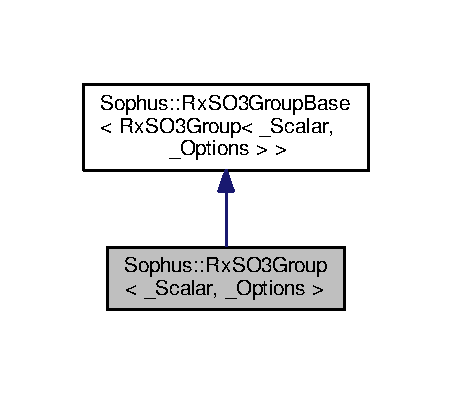
\includegraphics[width=217pt]{class_sophus_1_1_rx_s_o3_group__inherit__graph}
\end{center}
\end{figure}


Collaboration diagram for Sophus\+:\+:Rx\+S\+O3\+Group$<$ \+\_\+\+Scalar, \+\_\+\+Options $>$\+:
\nopagebreak
\begin{figure}[H]
\begin{center}
\leavevmode
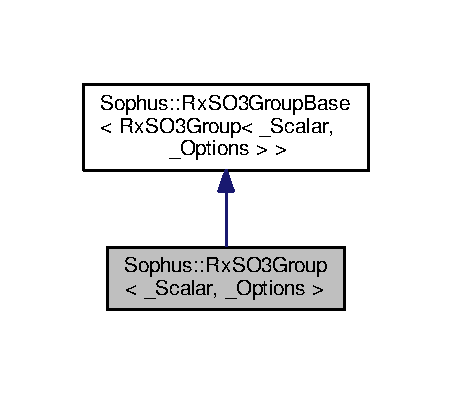
\includegraphics[width=217pt]{class_sophus_1_1_rx_s_o3_group__coll__graph}
\end{center}
\end{figure}
\subsection*{Public Types}
\begin{DoxyCompactItemize}
\item 
typedef internal\+::traits$<$ \hyperlink{class_sophus_1_1_s_o3_group}{S\+O3\+Group}$<$ \+\_\+\+Scalar, \+\_\+\+Options $>$ $>$\+::\hyperlink{class_sophus_1_1_rx_s_o3_group_a0c1248ba4deaab0ef231b74c60f77f87}{Scalar} \hyperlink{class_sophus_1_1_rx_s_o3_group_a0c1248ba4deaab0ef231b74c60f77f87}{Scalar}\hypertarget{class_sophus_1_1_rx_s_o3_group_a0c1248ba4deaab0ef231b74c60f77f87}{}\label{class_sophus_1_1_rx_s_o3_group_a0c1248ba4deaab0ef231b74c60f77f87}

\begin{DoxyCompactList}\small\item\em scalar type \end{DoxyCompactList}\item 
typedef internal\+::traits$<$ \hyperlink{class_sophus_1_1_s_o3_group}{S\+O3\+Group}$<$ \+\_\+\+Scalar, \+\_\+\+Options $>$ $>$\+::Quaternion\+Type \& \hyperlink{class_sophus_1_1_rx_s_o3_group_a01e579c31ebe7063ef5b737f53cd99cb}{Quaternion\+Reference}\hypertarget{class_sophus_1_1_rx_s_o3_group_a01e579c31ebe7063ef5b737f53cd99cb}{}\label{class_sophus_1_1_rx_s_o3_group_a01e579c31ebe7063ef5b737f53cd99cb}

\begin{DoxyCompactList}\small\item\em quaternion reference type \end{DoxyCompactList}\item 
typedef const internal\+::traits$<$ \hyperlink{class_sophus_1_1_s_o3_group}{S\+O3\+Group}$<$ \+\_\+\+Scalar, \+\_\+\+Options $>$ $>$\+::Quaternion\+Type \& \hyperlink{class_sophus_1_1_rx_s_o3_group_a03c34f6992514111a4fb03a1edce083f}{Const\+Quaternion\+Reference}\hypertarget{class_sophus_1_1_rx_s_o3_group_a03c34f6992514111a4fb03a1edce083f}{}\label{class_sophus_1_1_rx_s_o3_group_a03c34f6992514111a4fb03a1edce083f}

\begin{DoxyCompactList}\small\item\em quaternion const reference type \end{DoxyCompactList}\item 
typedef \hyperlink{class_sophus_1_1_rx_s_o3_group_base_a60b2d8cd20692d3d39e5e7c729d95145}{Base\+::\+Transformation} \hyperlink{class_sophus_1_1_rx_s_o3_group_ac8c43cedd9690622ff696fd1473fdfce}{Transformation}\hypertarget{class_sophus_1_1_rx_s_o3_group_ac8c43cedd9690622ff696fd1473fdfce}{}\label{class_sophus_1_1_rx_s_o3_group_ac8c43cedd9690622ff696fd1473fdfce}

\begin{DoxyCompactList}\small\item\em group transfomation type \end{DoxyCompactList}\item 
typedef \hyperlink{class_sophus_1_1_rx_s_o3_group_base_ad2d1b35ab03f6e91a80c2e78f07114a0}{Base\+::\+Point} \hyperlink{class_sophus_1_1_rx_s_o3_group_a9f4f8102f5db086c0bd7a5009fd6b611}{Point}\hypertarget{class_sophus_1_1_rx_s_o3_group_a9f4f8102f5db086c0bd7a5009fd6b611}{}\label{class_sophus_1_1_rx_s_o3_group_a9f4f8102f5db086c0bd7a5009fd6b611}

\begin{DoxyCompactList}\small\item\em point type \end{DoxyCompactList}\item 
typedef \hyperlink{class_sophus_1_1_rx_s_o3_group_base_aa1c4034b0a69496b28f1e81fdc7510c5}{Base\+::\+Tangent} \hyperlink{class_sophus_1_1_rx_s_o3_group_ad2e6135eac9eeebda0ef8909b974897d}{Tangent}\hypertarget{class_sophus_1_1_rx_s_o3_group_ad2e6135eac9eeebda0ef8909b974897d}{}\label{class_sophus_1_1_rx_s_o3_group_ad2e6135eac9eeebda0ef8909b974897d}

\begin{DoxyCompactList}\small\item\em tangent vector type \end{DoxyCompactList}\item 
typedef \hyperlink{class_sophus_1_1_rx_s_o3_group_base_a3f7cc9982043bf0082b7946f566a8179}{Base\+::\+Adjoint} \hyperlink{class_sophus_1_1_rx_s_o3_group_aa2a2e8f4047a33bb2ccf8a802878544f}{Adjoint}\hypertarget{class_sophus_1_1_rx_s_o3_group_aa2a2e8f4047a33bb2ccf8a802878544f}{}\label{class_sophus_1_1_rx_s_o3_group_aa2a2e8f4047a33bb2ccf8a802878544f}

\begin{DoxyCompactList}\small\item\em adjoint transformation type \end{DoxyCompactList}\end{DoxyCompactItemize}
\subsection*{Public Member Functions}
\begin{DoxyCompactItemize}
\item 
E\+I\+G\+E\+N\+\_\+\+M\+A\+K\+E\+\_\+\+A\+L\+I\+G\+N\+E\+D\+\_\+\+O\+P\+E\+R\+A\+T\+O\+R\+\_\+\+N\+EW \hyperlink{class_sophus_1_1_rx_s_o3_group_aa8b27095237070c5cae830e49bb9c196}{Rx\+S\+O3\+Group} ()
\begin{DoxyCompactList}\small\item\em Default constructor. \end{DoxyCompactList}\item 
{\footnotesize template$<$typename Other\+Derived $>$ }\\\hyperlink{class_sophus_1_1_rx_s_o3_group_a970f9fc29a915d8036887f2f5991420d}{Rx\+S\+O3\+Group} (const \hyperlink{class_sophus_1_1_rx_s_o3_group_base}{Rx\+S\+O3\+Group\+Base}$<$ Other\+Derived $>$ \&other)\hypertarget{class_sophus_1_1_rx_s_o3_group_a970f9fc29a915d8036887f2f5991420d}{}\label{class_sophus_1_1_rx_s_o3_group_a970f9fc29a915d8036887f2f5991420d}

\begin{DoxyCompactList}\small\item\em Copy constructor. \end{DoxyCompactList}\item 
\hyperlink{class_sophus_1_1_rx_s_o3_group_ad271361baf1d50722638870defc9e575}{Rx\+S\+O3\+Group} (const \hyperlink{class_sophus_1_1_rx_s_o3_group_ac8c43cedd9690622ff696fd1473fdfce}{Transformation} \&sR)
\begin{DoxyCompactList}\small\item\em Constructor from scaled rotation matrix. \end{DoxyCompactList}\item 
\hyperlink{class_sophus_1_1_rx_s_o3_group_a602f7551e896428c8241331ae075416a}{Rx\+S\+O3\+Group} (const \hyperlink{class_sophus_1_1_rx_s_o3_group_a0c1248ba4deaab0ef231b74c60f77f87}{Scalar} \&\hyperlink{class_sophus_1_1_rx_s_o3_group_base_a568f5cbdc1a40cd0f6237a91da65cf4a}{scale}, const \hyperlink{class_sophus_1_1_rx_s_o3_group_ac8c43cedd9690622ff696fd1473fdfce}{Transformation} \&R)
\begin{DoxyCompactList}\small\item\em Constructor from scale factor and rotation matrix. \end{DoxyCompactList}\item 
\hyperlink{class_sophus_1_1_rx_s_o3_group_a39635b4b1f03eb43bb506b17b1bfe353}{Rx\+S\+O3\+Group} (const \hyperlink{class_sophus_1_1_rx_s_o3_group_a0c1248ba4deaab0ef231b74c60f77f87}{Scalar} \&\hyperlink{class_sophus_1_1_rx_s_o3_group_base_a568f5cbdc1a40cd0f6237a91da65cf4a}{scale}, const \hyperlink{class_sophus_1_1_s_o3_group}{S\+O3\+Group}$<$ \hyperlink{class_sophus_1_1_rx_s_o3_group_a0c1248ba4deaab0ef231b74c60f77f87}{Scalar} $>$ \&so3)
\begin{DoxyCompactList}\small\item\em Constructor from scale factor and S\+O3. \end{DoxyCompactList}\item 
\hyperlink{class_sophus_1_1_rx_s_o3_group_a1c709c4ea5da483f12b968abfdbee68c}{Rx\+S\+O3\+Group} (const Quaternion$<$ \hyperlink{class_sophus_1_1_rx_s_o3_group_a0c1248ba4deaab0ef231b74c60f77f87}{Scalar} $>$ \&quat)
\begin{DoxyCompactList}\small\item\em Constructor from quaternion. \end{DoxyCompactList}\item 
E\+I\+G\+E\+N\+\_\+\+S\+T\+R\+O\+N\+G\+\_\+\+I\+N\+L\+I\+NE \hyperlink{class_sophus_1_1_rx_s_o3_group_a01e579c31ebe7063ef5b737f53cd99cb}{Quaternion\+Reference} \hyperlink{class_sophus_1_1_rx_s_o3_group_add7f349475c8b3c92ebe761b47d62b31}{quaternion} ()\hypertarget{class_sophus_1_1_rx_s_o3_group_add7f349475c8b3c92ebe761b47d62b31}{}\label{class_sophus_1_1_rx_s_o3_group_add7f349475c8b3c92ebe761b47d62b31}

\begin{DoxyCompactList}\small\item\em Mutator of quaternion. \end{DoxyCompactList}\item 
E\+I\+G\+E\+N\+\_\+\+S\+T\+R\+O\+N\+G\+\_\+\+I\+N\+L\+I\+NE \hyperlink{class_sophus_1_1_rx_s_o3_group_a03c34f6992514111a4fb03a1edce083f}{Const\+Quaternion\+Reference} \hyperlink{class_sophus_1_1_rx_s_o3_group_a59656a350e486b5375b1bc5dfae8333a}{quaternion} () const \hypertarget{class_sophus_1_1_rx_s_o3_group_a59656a350e486b5375b1bc5dfae8333a}{}\label{class_sophus_1_1_rx_s_o3_group_a59656a350e486b5375b1bc5dfae8333a}

\begin{DoxyCompactList}\small\item\em Accessor of quaternion. \end{DoxyCompactList}\end{DoxyCompactItemize}
\subsection*{Static Public Attributes}
\begin{DoxyCompactItemize}
\item 
static const int \hyperlink{class_sophus_1_1_rx_s_o3_group_a4080b614adcd54d45e835b155717f4e7}{DoF} = Base\+::\+DoF\hypertarget{class_sophus_1_1_rx_s_o3_group_a4080b614adcd54d45e835b155717f4e7}{}\label{class_sophus_1_1_rx_s_o3_group_a4080b614adcd54d45e835b155717f4e7}

\begin{DoxyCompactList}\small\item\em degree of freedom of group \end{DoxyCompactList}\item 
static const int \hyperlink{class_sophus_1_1_rx_s_o3_group_a2338a5de2ec08107613f52f325e8d83c}{num\+\_\+parameters} = Base\+::num\+\_\+parameters\hypertarget{class_sophus_1_1_rx_s_o3_group_a2338a5de2ec08107613f52f325e8d83c}{}\label{class_sophus_1_1_rx_s_o3_group_a2338a5de2ec08107613f52f325e8d83c}

\begin{DoxyCompactList}\small\item\em number of internal parameters used \end{DoxyCompactList}\item 
static const int \hyperlink{class_sophus_1_1_rx_s_o3_group_a277309f659efc31d66f52a6f04dafcc0}{N} = Base\+::N\hypertarget{class_sophus_1_1_rx_s_o3_group_a277309f659efc31d66f52a6f04dafcc0}{}\label{class_sophus_1_1_rx_s_o3_group_a277309f659efc31d66f52a6f04dafcc0}

\begin{DoxyCompactList}\small\item\em group transformations are NxN matrices \end{DoxyCompactList}\end{DoxyCompactItemize}
\subsection*{Protected Attributes}
\begin{DoxyCompactItemize}
\item 
Quaternion$<$ \hyperlink{class_sophus_1_1_rx_s_o3_group_a0c1248ba4deaab0ef231b74c60f77f87}{Scalar} $>$ {\bfseries quaternion\+\_\+}\hypertarget{class_sophus_1_1_rx_s_o3_group_adcb39c00a0db2de7289a16a4bdf00f44}{}\label{class_sophus_1_1_rx_s_o3_group_adcb39c00a0db2de7289a16a4bdf00f44}

\end{DoxyCompactItemize}
\subsection*{Additional Inherited Members}


\subsection{Detailed Description}
\subsubsection*{template$<$typename \+\_\+\+Scalar, int \+\_\+\+Options$>$\\*
class Sophus\+::\+Rx\+S\+O3\+Group$<$ \+\_\+\+Scalar, \+\_\+\+Options $>$}

Rx\+S\+O3 default type -\/ Constructors and default storage for Rx\+S\+O3 Type. 

Definition at line 34 of file rxso3.\+hpp.



\subsection{Constructor \& Destructor Documentation}
\index{Sophus\+::\+Rx\+S\+O3\+Group@{Sophus\+::\+Rx\+S\+O3\+Group}!Rx\+S\+O3\+Group@{Rx\+S\+O3\+Group}}
\index{Rx\+S\+O3\+Group@{Rx\+S\+O3\+Group}!Sophus\+::\+Rx\+S\+O3\+Group@{Sophus\+::\+Rx\+S\+O3\+Group}}
\subsubsection[{\texorpdfstring{Rx\+S\+O3\+Group()}{RxSO3Group()}}]{\setlength{\rightskip}{0pt plus 5cm}template$<$typename \+\_\+\+Scalar, int \+\_\+\+Options$>$ E\+I\+G\+E\+N\+\_\+\+M\+A\+K\+E\+\_\+\+A\+L\+I\+G\+N\+E\+D\+\_\+\+O\+P\+E\+R\+A\+T\+O\+R\+\_\+\+N\+EW {\bf Sophus\+::\+Rx\+S\+O3\+Group}$<$ \+\_\+\+Scalar, \+\_\+\+Options $>$\+::{\bf Rx\+S\+O3\+Group} (
\begin{DoxyParamCaption}
{}
\end{DoxyParamCaption}
)\hspace{0.3cm}{\ttfamily [inline]}}\hypertarget{class_sophus_1_1_rx_s_o3_group_aa8b27095237070c5cae830e49bb9c196}{}\label{class_sophus_1_1_rx_s_o3_group_aa8b27095237070c5cae830e49bb9c196}


Default constructor. 

Initialize Quaternion to identity rotation and scale. 

Definition at line 623 of file rxso3.\+hpp.

\index{Sophus\+::\+Rx\+S\+O3\+Group@{Sophus\+::\+Rx\+S\+O3\+Group}!Rx\+S\+O3\+Group@{Rx\+S\+O3\+Group}}
\index{Rx\+S\+O3\+Group@{Rx\+S\+O3\+Group}!Sophus\+::\+Rx\+S\+O3\+Group@{Sophus\+::\+Rx\+S\+O3\+Group}}
\subsubsection[{\texorpdfstring{Rx\+S\+O3\+Group(const Transformation \&s\+R)}{RxSO3Group(const Transformation &sR)}}]{\setlength{\rightskip}{0pt plus 5cm}template$<$typename \+\_\+\+Scalar, int \+\_\+\+Options$>$ {\bf Sophus\+::\+Rx\+S\+O3\+Group}$<$ \+\_\+\+Scalar, \+\_\+\+Options $>$\+::{\bf Rx\+S\+O3\+Group} (
\begin{DoxyParamCaption}
\item[{const {\bf Transformation} \&}]{sR}
\end{DoxyParamCaption}
)\hspace{0.3cm}{\ttfamily [inline]}, {\ttfamily [explicit]}}\hypertarget{class_sophus_1_1_rx_s_o3_group_ad271361baf1d50722638870defc9e575}{}\label{class_sophus_1_1_rx_s_o3_group_ad271361baf1d50722638870defc9e575}


Constructor from scaled rotation matrix. 

\begin{DoxyPrecond}{Precondition}
matrix need to be \char`\"{}scaled orthogonal\char`\"{} with positive determinant 
\end{DoxyPrecond}


Definition at line 642 of file rxso3.\+hpp.

\index{Sophus\+::\+Rx\+S\+O3\+Group@{Sophus\+::\+Rx\+S\+O3\+Group}!Rx\+S\+O3\+Group@{Rx\+S\+O3\+Group}}
\index{Rx\+S\+O3\+Group@{Rx\+S\+O3\+Group}!Sophus\+::\+Rx\+S\+O3\+Group@{Sophus\+::\+Rx\+S\+O3\+Group}}
\subsubsection[{\texorpdfstring{Rx\+S\+O3\+Group(const Scalar \&scale, const Transformation \&\+R)}{RxSO3Group(const Scalar &scale, const Transformation &R)}}]{\setlength{\rightskip}{0pt plus 5cm}template$<$typename \+\_\+\+Scalar, int \+\_\+\+Options$>$ {\bf Sophus\+::\+Rx\+S\+O3\+Group}$<$ \+\_\+\+Scalar, \+\_\+\+Options $>$\+::{\bf Rx\+S\+O3\+Group} (
\begin{DoxyParamCaption}
\item[{const {\bf Scalar} \&}]{scale, }
\item[{const {\bf Transformation} \&}]{R}
\end{DoxyParamCaption}
)\hspace{0.3cm}{\ttfamily [inline]}}\hypertarget{class_sophus_1_1_rx_s_o3_group_a602f7551e896428c8241331ae075416a}{}\label{class_sophus_1_1_rx_s_o3_group_a602f7551e896428c8241331ae075416a}


Constructor from scale factor and rotation matrix. 

\begin{DoxyPrecond}{Precondition}
rotation matrix need to be orthogonal with determinant of 1 

scale need to be not zero 
\end{DoxyPrecond}


Definition at line 653 of file rxso3.\+hpp.

\index{Sophus\+::\+Rx\+S\+O3\+Group@{Sophus\+::\+Rx\+S\+O3\+Group}!Rx\+S\+O3\+Group@{Rx\+S\+O3\+Group}}
\index{Rx\+S\+O3\+Group@{Rx\+S\+O3\+Group}!Sophus\+::\+Rx\+S\+O3\+Group@{Sophus\+::\+Rx\+S\+O3\+Group}}
\subsubsection[{\texorpdfstring{Rx\+S\+O3\+Group(const Scalar \&scale, const S\+O3\+Group$<$ Scalar $>$ \&so3)}{RxSO3Group(const Scalar &scale, const SO3Group< Scalar > &so3)}}]{\setlength{\rightskip}{0pt plus 5cm}template$<$typename \+\_\+\+Scalar, int \+\_\+\+Options$>$ {\bf Sophus\+::\+Rx\+S\+O3\+Group}$<$ \+\_\+\+Scalar, \+\_\+\+Options $>$\+::{\bf Rx\+S\+O3\+Group} (
\begin{DoxyParamCaption}
\item[{const {\bf Scalar} \&}]{scale, }
\item[{const {\bf S\+O3\+Group}$<$ {\bf Scalar} $>$ \&}]{so3}
\end{DoxyParamCaption}
)\hspace{0.3cm}{\ttfamily [inline]}}\hypertarget{class_sophus_1_1_rx_s_o3_group_a39635b4b1f03eb43bb506b17b1bfe353}{}\label{class_sophus_1_1_rx_s_o3_group_a39635b4b1f03eb43bb506b17b1bfe353}


Constructor from scale factor and S\+O3. 

\begin{DoxyPrecond}{Precondition}
scale need to be not zero 
\end{DoxyPrecond}


Definition at line 668 of file rxso3.\+hpp.

\index{Sophus\+::\+Rx\+S\+O3\+Group@{Sophus\+::\+Rx\+S\+O3\+Group}!Rx\+S\+O3\+Group@{Rx\+S\+O3\+Group}}
\index{Rx\+S\+O3\+Group@{Rx\+S\+O3\+Group}!Sophus\+::\+Rx\+S\+O3\+Group@{Sophus\+::\+Rx\+S\+O3\+Group}}
\subsubsection[{\texorpdfstring{Rx\+S\+O3\+Group(const Quaternion$<$ Scalar $>$ \&quat)}{RxSO3Group(const Quaternion< Scalar > &quat)}}]{\setlength{\rightskip}{0pt plus 5cm}template$<$typename \+\_\+\+Scalar, int \+\_\+\+Options$>$ {\bf Sophus\+::\+Rx\+S\+O3\+Group}$<$ \+\_\+\+Scalar, \+\_\+\+Options $>$\+::{\bf Rx\+S\+O3\+Group} (
\begin{DoxyParamCaption}
\item[{const Quaternion$<$ {\bf Scalar} $>$ \&}]{quat}
\end{DoxyParamCaption}
)\hspace{0.3cm}{\ttfamily [inline]}, {\ttfamily [explicit]}}\hypertarget{class_sophus_1_1_rx_s_o3_group_a1c709c4ea5da483f12b968abfdbee68c}{}\label{class_sophus_1_1_rx_s_o3_group_a1c709c4ea5da483f12b968abfdbee68c}


Constructor from quaternion. 

\begin{DoxyPrecond}{Precondition}
quaternion must not be zero 
\end{DoxyPrecond}


Definition at line 683 of file rxso3.\+hpp.



The documentation for this class was generated from the following file\+:\begin{DoxyCompactItemize}
\item 
include/\+Sophus/sophus/rxso3.\+hpp\end{DoxyCompactItemize}

\hypertarget{class_sophus_1_1_rx_s_o3_group_base}{}\section{Sophus\+:\+:Rx\+S\+O3\+Group\+Base$<$ Derived $>$ Class Template Reference}
\label{class_sophus_1_1_rx_s_o3_group_base}\index{Sophus\+::\+Rx\+S\+O3\+Group\+Base$<$ Derived $>$@{Sophus\+::\+Rx\+S\+O3\+Group\+Base$<$ Derived $>$}}


Rx\+S\+O3 base type -\/ implements Rx\+S\+O3 class but is storage agnostic.  




{\ttfamily \#include $<$rxso3.\+hpp$>$}

\subsection*{Public Types}
\begin{DoxyCompactItemize}
\item 
typedef internal\+::traits$<$ Derived $>$\+::\hyperlink{class_sophus_1_1_rx_s_o3_group_base_af4006e7d95216a7e50823a1cd9c9e265}{Scalar} \hyperlink{class_sophus_1_1_rx_s_o3_group_base_af4006e7d95216a7e50823a1cd9c9e265}{Scalar}\hypertarget{class_sophus_1_1_rx_s_o3_group_base_af4006e7d95216a7e50823a1cd9c9e265}{}\label{class_sophus_1_1_rx_s_o3_group_base_af4006e7d95216a7e50823a1cd9c9e265}

\begin{DoxyCompactList}\small\item\em scalar type, use with care since this might be a Map type \end{DoxyCompactList}\item 
typedef internal\+::traits$<$ Derived $>$\+::Quaternion\+Type \& \hyperlink{class_sophus_1_1_rx_s_o3_group_base_a3575bb8e7108073f73835ed59623d94a}{Quaternion\+Reference}\hypertarget{class_sophus_1_1_rx_s_o3_group_base_a3575bb8e7108073f73835ed59623d94a}{}\label{class_sophus_1_1_rx_s_o3_group_base_a3575bb8e7108073f73835ed59623d94a}

\begin{DoxyCompactList}\small\item\em quaternion reference type \end{DoxyCompactList}\item 
typedef const internal\+::traits$<$ Derived $>$\+::Quaternion\+Type \& \hyperlink{class_sophus_1_1_rx_s_o3_group_base_a3f2849c5a1cea4f295be3f149a4eee6d}{Const\+Quaternion\+Reference}\hypertarget{class_sophus_1_1_rx_s_o3_group_base_a3f2849c5a1cea4f295be3f149a4eee6d}{}\label{class_sophus_1_1_rx_s_o3_group_base_a3f2849c5a1cea4f295be3f149a4eee6d}

\begin{DoxyCompactList}\small\item\em quaternion const reference type \end{DoxyCompactList}\item 
typedef Matrix$<$ \hyperlink{class_sophus_1_1_rx_s_o3_group_base_af4006e7d95216a7e50823a1cd9c9e265}{Scalar}, \hyperlink{class_sophus_1_1_rx_s_o3_group_base_ab35c867a7781b1993f12ac6cb2fdf80b}{N}, \hyperlink{class_sophus_1_1_rx_s_o3_group_base_ab35c867a7781b1993f12ac6cb2fdf80b}{N} $>$ \hyperlink{class_sophus_1_1_rx_s_o3_group_base_a60b2d8cd20692d3d39e5e7c729d95145}{Transformation}\hypertarget{class_sophus_1_1_rx_s_o3_group_base_a60b2d8cd20692d3d39e5e7c729d95145}{}\label{class_sophus_1_1_rx_s_o3_group_base_a60b2d8cd20692d3d39e5e7c729d95145}

\begin{DoxyCompactList}\small\item\em group transfomation type \end{DoxyCompactList}\item 
typedef Matrix$<$ \hyperlink{class_sophus_1_1_rx_s_o3_group_base_af4006e7d95216a7e50823a1cd9c9e265}{Scalar}, 3, 1 $>$ \hyperlink{class_sophus_1_1_rx_s_o3_group_base_ad2d1b35ab03f6e91a80c2e78f07114a0}{Point}\hypertarget{class_sophus_1_1_rx_s_o3_group_base_ad2d1b35ab03f6e91a80c2e78f07114a0}{}\label{class_sophus_1_1_rx_s_o3_group_base_ad2d1b35ab03f6e91a80c2e78f07114a0}

\begin{DoxyCompactList}\small\item\em point type \end{DoxyCompactList}\item 
typedef Matrix$<$ \hyperlink{class_sophus_1_1_rx_s_o3_group_base_af4006e7d95216a7e50823a1cd9c9e265}{Scalar}, \hyperlink{class_sophus_1_1_rx_s_o3_group_base_a04536baf7b3670c95ccaef37d7105ba1}{DoF}, 1 $>$ \hyperlink{class_sophus_1_1_rx_s_o3_group_base_aa1c4034b0a69496b28f1e81fdc7510c5}{Tangent}\hypertarget{class_sophus_1_1_rx_s_o3_group_base_aa1c4034b0a69496b28f1e81fdc7510c5}{}\label{class_sophus_1_1_rx_s_o3_group_base_aa1c4034b0a69496b28f1e81fdc7510c5}

\begin{DoxyCompactList}\small\item\em tangent vector type \end{DoxyCompactList}\item 
typedef Matrix$<$ \hyperlink{class_sophus_1_1_rx_s_o3_group_base_af4006e7d95216a7e50823a1cd9c9e265}{Scalar}, \hyperlink{class_sophus_1_1_rx_s_o3_group_base_a04536baf7b3670c95ccaef37d7105ba1}{DoF}, \hyperlink{class_sophus_1_1_rx_s_o3_group_base_a04536baf7b3670c95ccaef37d7105ba1}{DoF} $>$ \hyperlink{class_sophus_1_1_rx_s_o3_group_base_a3f7cc9982043bf0082b7946f566a8179}{Adjoint}\hypertarget{class_sophus_1_1_rx_s_o3_group_base_a3f7cc9982043bf0082b7946f566a8179}{}\label{class_sophus_1_1_rx_s_o3_group_base_a3f7cc9982043bf0082b7946f566a8179}

\begin{DoxyCompactList}\small\item\em adjoint transformation type \end{DoxyCompactList}\end{DoxyCompactItemize}
\subsection*{Public Member Functions}
\begin{DoxyCompactItemize}
\item 
const \hyperlink{class_sophus_1_1_rx_s_o3_group_base_a3f7cc9982043bf0082b7946f566a8179}{Adjoint} \hyperlink{class_sophus_1_1_rx_s_o3_group_base_a905a15824f72eeae9fcba7d2eec00c4c}{Adj} () const 
\begin{DoxyCompactList}\small\item\em Adjoint transformation. \end{DoxyCompactList}\item 
{\footnotesize template$<$typename New\+Scalar\+Type $>$ }\\\hyperlink{class_sophus_1_1_rx_s_o3_group}{Rx\+S\+O3\+Group}$<$ New\+Scalar\+Type $>$ \hyperlink{class_sophus_1_1_rx_s_o3_group_base_abef15272073c5590bd914655b176874d}{cast} () const 
\item 
\hyperlink{class_sophus_1_1_rx_s_o3_group_base_af4006e7d95216a7e50823a1cd9c9e265}{Scalar} $\ast$ \hyperlink{class_sophus_1_1_rx_s_o3_group_base_a518457683a0b4b89ea6435579b3455f9}{data} ()
\item 
const \hyperlink{class_sophus_1_1_rx_s_o3_group_base_af4006e7d95216a7e50823a1cd9c9e265}{Scalar} $\ast$ \hyperlink{class_sophus_1_1_rx_s_o3_group_base_af9375223fdd4e0ac9b3866730800c0ba}{data} () const 
\item 
void \hyperlink{class_sophus_1_1_rx_s_o3_group_base_adc77a40831c4a064ef833e7697152e98}{fast\+Multiply} (const \hyperlink{class_sophus_1_1_rx_s_o3_group}{Rx\+S\+O3\+Group}$<$ \hyperlink{class_sophus_1_1_rx_s_o3_group_base_af4006e7d95216a7e50823a1cd9c9e265}{Scalar} $>$ \&other)
\begin{DoxyCompactList}\small\item\em In-\/place group multiplication. \end{DoxyCompactList}\item 
const \hyperlink{class_sophus_1_1_rx_s_o3_group}{Rx\+S\+O3\+Group}$<$ \hyperlink{class_sophus_1_1_rx_s_o3_group_base_af4006e7d95216a7e50823a1cd9c9e265}{Scalar} $>$ \hyperlink{class_sophus_1_1_rx_s_o3_group_base_a3b47ec202990b4bd08859feafdca1cef}{inverse} () const 
\item 
const \hyperlink{class_sophus_1_1_rx_s_o3_group_base_aa1c4034b0a69496b28f1e81fdc7510c5}{Tangent} \hyperlink{class_sophus_1_1_rx_s_o3_group_base_aa201b101217eb02366ae02d423a1ef0d}{log} () const 
\begin{DoxyCompactList}\small\item\em Logarithmic map. \end{DoxyCompactList}\item 
const \hyperlink{class_sophus_1_1_rx_s_o3_group_base_a60b2d8cd20692d3d39e5e7c729d95145}{Transformation} \hyperlink{class_sophus_1_1_rx_s_o3_group_base_ae2fcf316d587e4bedba18125149f4f14}{matrix} () const 
\item 
{\footnotesize template$<$typename Other\+Derived $>$ }\\\hyperlink{class_sophus_1_1_rx_s_o3_group_base}{Rx\+S\+O3\+Group\+Base}$<$ Derived $>$ \& \hyperlink{class_sophus_1_1_rx_s_o3_group_base_adaef92c98a49d7eeb559b531c58324e1}{operator=} (const \hyperlink{class_sophus_1_1_rx_s_o3_group_base}{Rx\+S\+O3\+Group\+Base}$<$ Other\+Derived $>$ \&other)\hypertarget{class_sophus_1_1_rx_s_o3_group_base_adaef92c98a49d7eeb559b531c58324e1}{}\label{class_sophus_1_1_rx_s_o3_group_base_adaef92c98a49d7eeb559b531c58324e1}

\begin{DoxyCompactList}\small\item\em Assignment operator. \end{DoxyCompactList}\item 
const \hyperlink{class_sophus_1_1_rx_s_o3_group}{Rx\+S\+O3\+Group}$<$ \hyperlink{class_sophus_1_1_rx_s_o3_group_base_af4006e7d95216a7e50823a1cd9c9e265}{Scalar} $>$ \hyperlink{class_sophus_1_1_rx_s_o3_group_base_a26b9ea82336b1857f4a9cd9c66b51b1e}{operator$\ast$} (const \hyperlink{class_sophus_1_1_rx_s_o3_group}{Rx\+S\+O3\+Group}$<$ \hyperlink{class_sophus_1_1_rx_s_o3_group_base_af4006e7d95216a7e50823a1cd9c9e265}{Scalar} $>$ \&other) const 
\begin{DoxyCompactList}\small\item\em Group multiplication. \end{DoxyCompactList}\item 
const \hyperlink{class_sophus_1_1_rx_s_o3_group_base_ad2d1b35ab03f6e91a80c2e78f07114a0}{Point} \hyperlink{class_sophus_1_1_rx_s_o3_group_base_a464df8f39a1f89f865ce7bb02e1154ec}{operator$\ast$} (const \hyperlink{class_sophus_1_1_rx_s_o3_group_base_ad2d1b35ab03f6e91a80c2e78f07114a0}{Point} \&p) const 
\begin{DoxyCompactList}\small\item\em Group action on $ \mathbf{R}^3 $. \end{DoxyCompactList}\item 
void \hyperlink{class_sophus_1_1_rx_s_o3_group_base_a91b5b4541313ce867db3b96dadf1cdb1}{operator$\ast$=} (const \hyperlink{class_sophus_1_1_rx_s_o3_group}{Rx\+S\+O3\+Group}$<$ \hyperlink{class_sophus_1_1_rx_s_o3_group_base_af4006e7d95216a7e50823a1cd9c9e265}{Scalar} $>$ \&other)
\begin{DoxyCompactList}\small\item\em In-\/place group multiplication. \end{DoxyCompactList}\item 
E\+I\+G\+E\+N\+\_\+\+S\+T\+R\+O\+N\+G\+\_\+\+I\+N\+L\+I\+NE \hyperlink{class_sophus_1_1_rx_s_o3_group_base_a3575bb8e7108073f73835ed59623d94a}{Quaternion\+Reference} \hyperlink{class_sophus_1_1_rx_s_o3_group_base_aec68e74ddebe953b41fc7ec597fde9ed}{quaternion} ()\hypertarget{class_sophus_1_1_rx_s_o3_group_base_aec68e74ddebe953b41fc7ec597fde9ed}{}\label{class_sophus_1_1_rx_s_o3_group_base_aec68e74ddebe953b41fc7ec597fde9ed}

\begin{DoxyCompactList}\small\item\em Mutator of quaternion. \end{DoxyCompactList}\item 
E\+I\+G\+E\+N\+\_\+\+S\+T\+R\+O\+N\+G\+\_\+\+I\+N\+L\+I\+NE \hyperlink{class_sophus_1_1_rx_s_o3_group_base_a3f2849c5a1cea4f295be3f149a4eee6d}{Const\+Quaternion\+Reference} \hyperlink{class_sophus_1_1_rx_s_o3_group_base_a1bd73e5ff76441f3f5321f8fa0d95f4d}{quaternion} () const \hypertarget{class_sophus_1_1_rx_s_o3_group_base_a1bd73e5ff76441f3f5321f8fa0d95f4d}{}\label{class_sophus_1_1_rx_s_o3_group_base_a1bd73e5ff76441f3f5321f8fa0d95f4d}

\begin{DoxyCompactList}\small\item\em Accessor of quaternion. \end{DoxyCompactList}\item 
\hyperlink{class_sophus_1_1_rx_s_o3_group_base_a60b2d8cd20692d3d39e5e7c729d95145}{Transformation} \hyperlink{class_sophus_1_1_rx_s_o3_group_base_a18c5fc6302987791964ba51371efa6be}{rotation\+Matrix} () const 
\item 
E\+I\+G\+E\+N\+\_\+\+S\+T\+R\+O\+N\+G\+\_\+\+I\+N\+L\+I\+NE const \hyperlink{class_sophus_1_1_rx_s_o3_group_base_af4006e7d95216a7e50823a1cd9c9e265}{Scalar} \hyperlink{class_sophus_1_1_rx_s_o3_group_base_a568f5cbdc1a40cd0f6237a91da65cf4a}{scale} () const 
\item 
void \hyperlink{class_sophus_1_1_rx_s_o3_group_base_a657f576a0239d2ce6aba46f48d904c1f}{set\+Rotation\+Matrix} (const \hyperlink{class_sophus_1_1_rx_s_o3_group_base_a60b2d8cd20692d3d39e5e7c729d95145}{Transformation} \&R)
\begin{DoxyCompactList}\small\item\em Setter of quaternion using rotation matrix, leaves scale untouched. \end{DoxyCompactList}\item 
E\+I\+G\+E\+N\+\_\+\+S\+T\+R\+O\+N\+G\+\_\+\+I\+N\+L\+I\+NE void \hyperlink{class_sophus_1_1_rx_s_o3_group_base_aa0481ad33d7fd4f8698c05bbfc62422e}{set\+Scale} (const \hyperlink{class_sophus_1_1_rx_s_o3_group_base_af4006e7d95216a7e50823a1cd9c9e265}{Scalar} \&\hyperlink{class_sophus_1_1_rx_s_o3_group_base_a568f5cbdc1a40cd0f6237a91da65cf4a}{scale})\hypertarget{class_sophus_1_1_rx_s_o3_group_base_aa0481ad33d7fd4f8698c05bbfc62422e}{}\label{class_sophus_1_1_rx_s_o3_group_base_aa0481ad33d7fd4f8698c05bbfc62422e}

\begin{DoxyCompactList}\small\item\em Scale setter. \end{DoxyCompactList}\item 
void \hyperlink{class_sophus_1_1_rx_s_o3_group_base_ae05c6ad0bd43144e8446b103bfcdbbfd}{set\+Scaled\+Rotation\+Matrix} (const \hyperlink{class_sophus_1_1_rx_s_o3_group_base_a60b2d8cd20692d3d39e5e7c729d95145}{Transformation} \&sR)
\begin{DoxyCompactList}\small\item\em Setter of quaternion using scaled rotation matrix. \end{DoxyCompactList}\end{DoxyCompactItemize}
\subsection*{Static Public Member Functions}
\begin{DoxyCompactItemize}
\item 
static const \hyperlink{class_sophus_1_1_rx_s_o3_group_base_a3f7cc9982043bf0082b7946f566a8179}{Adjoint} \hyperlink{class_sophus_1_1_rx_s_o3_group_base_a37ab5a127ff1e1520f9a5c2482ecb6ab}{d\+\_\+lie\+Bracketab\+\_\+by\+\_\+d\+\_\+a} (const \hyperlink{class_sophus_1_1_rx_s_o3_group_base_aa1c4034b0a69496b28f1e81fdc7510c5}{Tangent} \&b)
\item 
static const \hyperlink{class_sophus_1_1_rx_s_o3_group}{Rx\+S\+O3\+Group}$<$ \hyperlink{class_sophus_1_1_rx_s_o3_group_base_af4006e7d95216a7e50823a1cd9c9e265}{Scalar} $>$ \hyperlink{class_sophus_1_1_rx_s_o3_group_base_a74aa48955af3292059cdff7bec54480a}{exp} (const \hyperlink{class_sophus_1_1_rx_s_o3_group_base_aa1c4034b0a69496b28f1e81fdc7510c5}{Tangent} \&a)
\begin{DoxyCompactList}\small\item\em Group exponential. \end{DoxyCompactList}\item 
static const \hyperlink{class_sophus_1_1_rx_s_o3_group}{Rx\+S\+O3\+Group}$<$ \hyperlink{class_sophus_1_1_rx_s_o3_group_base_af4006e7d95216a7e50823a1cd9c9e265}{Scalar} $>$ \hyperlink{class_sophus_1_1_rx_s_o3_group_base_a64b2d932b458b49e01ffef1dfb789321}{exp\+And\+Theta} (const \hyperlink{class_sophus_1_1_rx_s_o3_group_base_aa1c4034b0a69496b28f1e81fdc7510c5}{Tangent} \&a, \hyperlink{class_sophus_1_1_rx_s_o3_group_base_af4006e7d95216a7e50823a1cd9c9e265}{Scalar} $\ast$theta)
\begin{DoxyCompactList}\small\item\em Group exponential and theta. \end{DoxyCompactList}\item 
static const \hyperlink{class_sophus_1_1_rx_s_o3_group_base_a60b2d8cd20692d3d39e5e7c729d95145}{Transformation} \hyperlink{class_sophus_1_1_rx_s_o3_group_base_ac6201edf006ea3b099317b6571a885fb}{generator} (int i)
\begin{DoxyCompactList}\small\item\em Generators. \end{DoxyCompactList}\item 
static const \hyperlink{class_sophus_1_1_rx_s_o3_group_base_a60b2d8cd20692d3d39e5e7c729d95145}{Transformation} \hyperlink{class_sophus_1_1_rx_s_o3_group_base_a0158a3e783122fa4ee7833db12f09ffd}{hat} (const \hyperlink{class_sophus_1_1_rx_s_o3_group_base_aa1c4034b0a69496b28f1e81fdc7510c5}{Tangent} \&a)
\begin{DoxyCompactList}\small\item\em hat-\/operator \end{DoxyCompactList}\item 
static const \hyperlink{class_sophus_1_1_rx_s_o3_group_base_aa1c4034b0a69496b28f1e81fdc7510c5}{Tangent} \hyperlink{class_sophus_1_1_rx_s_o3_group_base_a46710014c6234b7e4a6239dc985b2a6b}{lie\+Bracket} (const \hyperlink{class_sophus_1_1_rx_s_o3_group_base_aa1c4034b0a69496b28f1e81fdc7510c5}{Tangent} \&a, const \hyperlink{class_sophus_1_1_rx_s_o3_group_base_aa1c4034b0a69496b28f1e81fdc7510c5}{Tangent} \&b)
\begin{DoxyCompactList}\small\item\em Lie bracket. \end{DoxyCompactList}\item 
static const \hyperlink{class_sophus_1_1_rx_s_o3_group_base_aa1c4034b0a69496b28f1e81fdc7510c5}{Tangent} \hyperlink{class_sophus_1_1_rx_s_o3_group_base_ad6fa243f3fb9ca940f87dccae4b8e8d8}{log} (const \hyperlink{class_sophus_1_1_rx_s_o3_group}{Rx\+S\+O3\+Group}$<$ \hyperlink{class_sophus_1_1_rx_s_o3_group_base_af4006e7d95216a7e50823a1cd9c9e265}{Scalar} $>$ \&other)
\begin{DoxyCompactList}\small\item\em Logarithmic map. \end{DoxyCompactList}\item 
static const \hyperlink{class_sophus_1_1_rx_s_o3_group_base_aa1c4034b0a69496b28f1e81fdc7510c5}{Tangent} \hyperlink{class_sophus_1_1_rx_s_o3_group_base_a75f2cac71d286305b4e175db01b5bfc9}{log\+And\+Theta} (const \hyperlink{class_sophus_1_1_rx_s_o3_group}{Rx\+S\+O3\+Group}$<$ \hyperlink{class_sophus_1_1_rx_s_o3_group_base_af4006e7d95216a7e50823a1cd9c9e265}{Scalar} $>$ \&other, \hyperlink{class_sophus_1_1_rx_s_o3_group_base_af4006e7d95216a7e50823a1cd9c9e265}{Scalar} $\ast$theta)
\begin{DoxyCompactList}\small\item\em Logarithmic map and theta. \end{DoxyCompactList}\item 
static const \hyperlink{class_sophus_1_1_rx_s_o3_group_base_aa1c4034b0a69496b28f1e81fdc7510c5}{Tangent} \hyperlink{class_sophus_1_1_rx_s_o3_group_base_ab4f9270e3f4588bb1d848604b848a9fe}{vee} (const \hyperlink{class_sophus_1_1_rx_s_o3_group_base_a60b2d8cd20692d3d39e5e7c729d95145}{Transformation} \&Omega)
\begin{DoxyCompactList}\small\item\em vee-\/operator \end{DoxyCompactList}\end{DoxyCompactItemize}
\subsection*{Static Public Attributes}
\begin{DoxyCompactItemize}
\item 
static const int \hyperlink{class_sophus_1_1_rx_s_o3_group_base_a04536baf7b3670c95ccaef37d7105ba1}{DoF} = 4\hypertarget{class_sophus_1_1_rx_s_o3_group_base_a04536baf7b3670c95ccaef37d7105ba1}{}\label{class_sophus_1_1_rx_s_o3_group_base_a04536baf7b3670c95ccaef37d7105ba1}

\begin{DoxyCompactList}\small\item\em degree of freedom of group (three for rotation and one for scaling) \end{DoxyCompactList}\item 
static const int \hyperlink{class_sophus_1_1_rx_s_o3_group_base_a19a6866f0ec97d0abcc3fda1de37215d}{num\+\_\+parameters} = 4\hypertarget{class_sophus_1_1_rx_s_o3_group_base_a19a6866f0ec97d0abcc3fda1de37215d}{}\label{class_sophus_1_1_rx_s_o3_group_base_a19a6866f0ec97d0abcc3fda1de37215d}

\begin{DoxyCompactList}\small\item\em number of internal parameters used (quaternion for rotation and scaling) \end{DoxyCompactList}\item 
static const int \hyperlink{class_sophus_1_1_rx_s_o3_group_base_ab35c867a7781b1993f12ac6cb2fdf80b}{N} = 3\hypertarget{class_sophus_1_1_rx_s_o3_group_base_ab35c867a7781b1993f12ac6cb2fdf80b}{}\label{class_sophus_1_1_rx_s_o3_group_base_ab35c867a7781b1993f12ac6cb2fdf80b}

\begin{DoxyCompactList}\small\item\em group transformations are NxN matrices \end{DoxyCompactList}\end{DoxyCompactItemize}


\subsection{Detailed Description}
\subsubsection*{template$<$typename Derived$>$\\*
class Sophus\+::\+Rx\+S\+O3\+Group\+Base$<$ Derived $>$}

Rx\+S\+O3 base type -\/ implements Rx\+S\+O3 class but is storage agnostic. 

This class implements the group $ R^{+} \times SO3 $ (Rx\+S\+O3), the direct product of the group of positive scalar matrices (=isomorph to the positive real numbers) and the three-\/dimensional special orthogonal group S\+O3. Geometrically, it is the group of rotation and scaling in three dimensions. As a matrix groups, Rx\+S\+O3 consists of matrices of the form $ s\cdot R $ where $ R $ is an orthognal matrix with $ det(R)=1 $ and $ s>0 $ be a positive real number.

Internally, Rx\+S\+O3 is represented by the group of non-\/zero quaternions. This is a most compact representation since the degrees of freedom (DoF) of Rx\+S\+O3 (=4) equals the number of internal parameters (=4).

\mbox{[}add more detailed description/tutorial\mbox{]} 

Definition at line 98 of file rxso3.\+hpp.



\subsection{Member Function Documentation}
\index{Sophus\+::\+Rx\+S\+O3\+Group\+Base@{Sophus\+::\+Rx\+S\+O3\+Group\+Base}!Adj@{Adj}}
\index{Adj@{Adj}!Sophus\+::\+Rx\+S\+O3\+Group\+Base@{Sophus\+::\+Rx\+S\+O3\+Group\+Base}}
\subsubsection[{\texorpdfstring{Adj() const }{Adj() const }}]{\setlength{\rightskip}{0pt plus 5cm}template$<$typename Derived$>$ const {\bf Adjoint} {\bf Sophus\+::\+Rx\+S\+O3\+Group\+Base}$<$ Derived $>$\+::Adj (
\begin{DoxyParamCaption}
{}
\end{DoxyParamCaption}
) const\hspace{0.3cm}{\ttfamily [inline]}}\hypertarget{class_sophus_1_1_rx_s_o3_group_base_a905a15824f72eeae9fcba7d2eec00c4c}{}\label{class_sophus_1_1_rx_s_o3_group_base_a905a15824f72eeae9fcba7d2eec00c4c}


Adjoint transformation. 

This function return the adjoint transformation $ Ad $ of the group instance $ A $ such that for all $ x $ it holds that $ \widehat{Ad_A\cdot x} = A\widehat{x}A^{-1} $ with $\ \widehat{\cdot} $ being the \hyperlink{class_sophus_1_1_rx_s_o3_group_base_a0158a3e783122fa4ee7833db12f09ffd}{hat()}-\/operator.

For Rx\+S\+O3, it simply returns the rotation matrix corresponding to $ A $. 

Definition at line 140 of file rxso3.\+hpp.

\index{Sophus\+::\+Rx\+S\+O3\+Group\+Base@{Sophus\+::\+Rx\+S\+O3\+Group\+Base}!cast@{cast}}
\index{cast@{cast}!Sophus\+::\+Rx\+S\+O3\+Group\+Base@{Sophus\+::\+Rx\+S\+O3\+Group\+Base}}
\subsubsection[{\texorpdfstring{cast() const }{cast() const }}]{\setlength{\rightskip}{0pt plus 5cm}template$<$typename Derived$>$ template$<$typename New\+Scalar\+Type $>$ {\bf Rx\+S\+O3\+Group}$<$New\+Scalar\+Type$>$ {\bf Sophus\+::\+Rx\+S\+O3\+Group\+Base}$<$ Derived $>$\+::cast (
\begin{DoxyParamCaption}
{}
\end{DoxyParamCaption}
) const\hspace{0.3cm}{\ttfamily [inline]}}\hypertarget{class_sophus_1_1_rx_s_o3_group_base_abef15272073c5590bd914655b176874d}{}\label{class_sophus_1_1_rx_s_o3_group_base_abef15272073c5590bd914655b176874d}
\begin{DoxyReturn}{Returns}
copy of instance casted to New\+Scalar\+Type 
\end{DoxyReturn}


Definition at line 151 of file rxso3.\+hpp.

\index{Sophus\+::\+Rx\+S\+O3\+Group\+Base@{Sophus\+::\+Rx\+S\+O3\+Group\+Base}!d\+\_\+lie\+Bracketab\+\_\+by\+\_\+d\+\_\+a@{d\+\_\+lie\+Bracketab\+\_\+by\+\_\+d\+\_\+a}}
\index{d\+\_\+lie\+Bracketab\+\_\+by\+\_\+d\+\_\+a@{d\+\_\+lie\+Bracketab\+\_\+by\+\_\+d\+\_\+a}!Sophus\+::\+Rx\+S\+O3\+Group\+Base@{Sophus\+::\+Rx\+S\+O3\+Group\+Base}}
\subsubsection[{\texorpdfstring{d\+\_\+lie\+Bracketab\+\_\+by\+\_\+d\+\_\+a(const Tangent \&b)}{d_lieBracketab_by_d_a(const Tangent &b)}}]{\setlength{\rightskip}{0pt plus 5cm}template$<$typename Derived$>$ static const {\bf Adjoint} {\bf Sophus\+::\+Rx\+S\+O3\+Group\+Base}$<$ Derived $>$\+::d\+\_\+lie\+Bracketab\+\_\+by\+\_\+d\+\_\+a (
\begin{DoxyParamCaption}
\item[{const {\bf Tangent} \&}]{b}
\end{DoxyParamCaption}
)\hspace{0.3cm}{\ttfamily [inline]}, {\ttfamily [static]}}\hypertarget{class_sophus_1_1_rx_s_o3_group_base_a37ab5a127ff1e1520f9a5c2482ecb6ab}{}\label{class_sophus_1_1_rx_s_o3_group_base_a37ab5a127ff1e1520f9a5c2482ecb6ab}

\begin{DoxyParams}{Parameters}
{\em b} & 4-\/vector representation of Lie algebra element \\
\hline
\end{DoxyParams}
\begin{DoxyReturn}{Returns}
derivative of Lie bracket
\end{DoxyReturn}
This function returns $ \frac{\partial}{\partial a} [a, b]_{rxso3} $ with $ [a, b]_{rxso3} $ being the \hyperlink{class_sophus_1_1_rx_s_o3_group_base_a46710014c6234b7e4a6239dc985b2a6b}{lie\+Bracket()} of the Lie algebra rxso3.

\begin{DoxySeeAlso}{See also}
\hyperlink{class_sophus_1_1_rx_s_o3_group_base_a46710014c6234b7e4a6239dc985b2a6b}{lie\+Bracket()} 
\end{DoxySeeAlso}


Definition at line 377 of file rxso3.\+hpp.

\index{Sophus\+::\+Rx\+S\+O3\+Group\+Base@{Sophus\+::\+Rx\+S\+O3\+Group\+Base}!data@{data}}
\index{data@{data}!Sophus\+::\+Rx\+S\+O3\+Group\+Base@{Sophus\+::\+Rx\+S\+O3\+Group\+Base}}
\subsubsection[{\texorpdfstring{data()}{data()}}]{\setlength{\rightskip}{0pt plus 5cm}template$<$typename Derived$>$ {\bf Scalar}$\ast$ {\bf Sophus\+::\+Rx\+S\+O3\+Group\+Base}$<$ Derived $>$\+::data (
\begin{DoxyParamCaption}
{}
\end{DoxyParamCaption}
)\hspace{0.3cm}{\ttfamily [inline]}}\hypertarget{class_sophus_1_1_rx_s_o3_group_base_a518457683a0b4b89ea6435579b3455f9}{}\label{class_sophus_1_1_rx_s_o3_group_base_a518457683a0b4b89ea6435579b3455f9}
\begin{DoxyReturn}{Returns}
pointer to internal data
\end{DoxyReturn}
This provides direct read/write access to internal data. Rx\+S\+O3 is represented by an Eigen\+::\+Quaternion (four parameters).

Note\+: The first three Scalars represent the imaginary parts, while the forth Scalar represent the real part. 

Definition at line 165 of file rxso3.\+hpp.

\index{Sophus\+::\+Rx\+S\+O3\+Group\+Base@{Sophus\+::\+Rx\+S\+O3\+Group\+Base}!data@{data}}
\index{data@{data}!Sophus\+::\+Rx\+S\+O3\+Group\+Base@{Sophus\+::\+Rx\+S\+O3\+Group\+Base}}
\subsubsection[{\texorpdfstring{data() const }{data() const }}]{\setlength{\rightskip}{0pt plus 5cm}template$<$typename Derived$>$ const {\bf Scalar}$\ast$ {\bf Sophus\+::\+Rx\+S\+O3\+Group\+Base}$<$ Derived $>$\+::data (
\begin{DoxyParamCaption}
{}
\end{DoxyParamCaption}
) const\hspace{0.3cm}{\ttfamily [inline]}}\hypertarget{class_sophus_1_1_rx_s_o3_group_base_af9375223fdd4e0ac9b3866730800c0ba}{}\label{class_sophus_1_1_rx_s_o3_group_base_af9375223fdd4e0ac9b3866730800c0ba}
\begin{DoxyReturn}{Returns}
const pointer to internal data
\end{DoxyReturn}
Const version of \hyperlink{class_sophus_1_1_rx_s_o3_group_base_a518457683a0b4b89ea6435579b3455f9}{data()}. 

Definition at line 174 of file rxso3.\+hpp.

\index{Sophus\+::\+Rx\+S\+O3\+Group\+Base@{Sophus\+::\+Rx\+S\+O3\+Group\+Base}!exp@{exp}}
\index{exp@{exp}!Sophus\+::\+Rx\+S\+O3\+Group\+Base@{Sophus\+::\+Rx\+S\+O3\+Group\+Base}}
\subsubsection[{\texorpdfstring{exp(const Tangent \&a)}{exp(const Tangent &a)}}]{\setlength{\rightskip}{0pt plus 5cm}template$<$typename Derived$>$ static const {\bf Rx\+S\+O3\+Group}$<${\bf Scalar}$>$ {\bf Sophus\+::\+Rx\+S\+O3\+Group\+Base}$<$ Derived $>$\+::exp (
\begin{DoxyParamCaption}
\item[{const {\bf Tangent} \&}]{a}
\end{DoxyParamCaption}
)\hspace{0.3cm}{\ttfamily [inline]}, {\ttfamily [static]}}\hypertarget{class_sophus_1_1_rx_s_o3_group_base_a74aa48955af3292059cdff7bec54480a}{}\label{class_sophus_1_1_rx_s_o3_group_base_a74aa48955af3292059cdff7bec54480a}


Group exponential. 


\begin{DoxyParams}{Parameters}
{\em a} & tangent space element (rotation vector $ \omega $ and logarithm of scale) \\
\hline
\end{DoxyParams}
\begin{DoxyReturn}{Returns}
corresponding element of the group Rx\+S\+O3
\end{DoxyReturn}
To be more specific, this function computes $ \exp(\widehat{a}) $ with $ \exp(\cdot) $ being the matrix exponential and $ \widehat{\cdot} $ the \hyperlink{class_sophus_1_1_rx_s_o3_group_base_a0158a3e783122fa4ee7833db12f09ffd}{hat()}-\/operator of Rx\+S\+O3.

\begin{DoxySeeAlso}{See also}
\hyperlink{class_sophus_1_1_rx_s_o3_group_base_a64b2d932b458b49e01ffef1dfb789321}{exp\+And\+Theta()} 

\hyperlink{class_sophus_1_1_rx_s_o3_group_base_a0158a3e783122fa4ee7833db12f09ffd}{hat()} 

\hyperlink{class_sophus_1_1_rx_s_o3_group_base_aa201b101217eb02366ae02d423a1ef0d}{log()} 
\end{DoxySeeAlso}


Definition at line 400 of file rxso3.\+hpp.

\index{Sophus\+::\+Rx\+S\+O3\+Group\+Base@{Sophus\+::\+Rx\+S\+O3\+Group\+Base}!exp\+And\+Theta@{exp\+And\+Theta}}
\index{exp\+And\+Theta@{exp\+And\+Theta}!Sophus\+::\+Rx\+S\+O3\+Group\+Base@{Sophus\+::\+Rx\+S\+O3\+Group\+Base}}
\subsubsection[{\texorpdfstring{exp\+And\+Theta(const Tangent \&a, Scalar $\ast$theta)}{expAndTheta(const Tangent &a, Scalar *theta)}}]{\setlength{\rightskip}{0pt plus 5cm}template$<$typename Derived$>$ static const {\bf Rx\+S\+O3\+Group}$<${\bf Scalar}$>$ {\bf Sophus\+::\+Rx\+S\+O3\+Group\+Base}$<$ Derived $>$\+::exp\+And\+Theta (
\begin{DoxyParamCaption}
\item[{const {\bf Tangent} \&}]{a, }
\item[{{\bf Scalar} $\ast$}]{theta}
\end{DoxyParamCaption}
)\hspace{0.3cm}{\ttfamily [inline]}, {\ttfamily [static]}}\hypertarget{class_sophus_1_1_rx_s_o3_group_base_a64b2d932b458b49e01ffef1dfb789321}{}\label{class_sophus_1_1_rx_s_o3_group_base_a64b2d932b458b49e01ffef1dfb789321}


Group exponential and theta. 


\begin{DoxyParams}[1]{Parameters}
 & {\em a} & tangent space element (rotation vector $ \omega $ and logarithm of scale ) \\
\hline
\mbox{\tt out}  & {\em theta} & angle of rotation $ \theta = |\omega| $ \\
\hline
\end{DoxyParams}
\begin{DoxyReturn}{Returns}
corresponding element of the group Rx\+S\+O3
\end{DoxyReturn}
\begin{DoxySeeAlso}{See also}
\hyperlink{class_sophus_1_1_rx_s_o3_group_base_a74aa48955af3292059cdff7bec54480a}{exp()} for details 
\end{DoxySeeAlso}


Definition at line 416 of file rxso3.\+hpp.

\index{Sophus\+::\+Rx\+S\+O3\+Group\+Base@{Sophus\+::\+Rx\+S\+O3\+Group\+Base}!fast\+Multiply@{fast\+Multiply}}
\index{fast\+Multiply@{fast\+Multiply}!Sophus\+::\+Rx\+S\+O3\+Group\+Base@{Sophus\+::\+Rx\+S\+O3\+Group\+Base}}
\subsubsection[{\texorpdfstring{fast\+Multiply(const Rx\+S\+O3\+Group$<$ Scalar $>$ \&other)}{fastMultiply(const RxSO3Group< Scalar > &other)}}]{\setlength{\rightskip}{0pt plus 5cm}template$<$typename Derived$>$ void {\bf Sophus\+::\+Rx\+S\+O3\+Group\+Base}$<$ Derived $>$\+::fast\+Multiply (
\begin{DoxyParamCaption}
\item[{const {\bf Rx\+S\+O3\+Group}$<$ {\bf Scalar} $>$ \&}]{other}
\end{DoxyParamCaption}
)\hspace{0.3cm}{\ttfamily [inline]}}\hypertarget{class_sophus_1_1_rx_s_o3_group_base_adc77a40831c4a064ef833e7697152e98}{}\label{class_sophus_1_1_rx_s_o3_group_base_adc77a40831c4a064ef833e7697152e98}


In-\/place group multiplication. 

Same as \hyperlink{class_sophus_1_1_rx_s_o3_group_base_a91b5b4541313ce867db3b96dadf1cdb1}{operator$\ast$=()} for Rx\+S\+O3.

\begin{DoxySeeAlso}{See also}
\hyperlink{class_sophus_1_1_rx_s_o3_group_base_a91b5b4541313ce867db3b96dadf1cdb1}{operator$\ast$=()} 
\end{DoxySeeAlso}


Definition at line 186 of file rxso3.\+hpp.

\index{Sophus\+::\+Rx\+S\+O3\+Group\+Base@{Sophus\+::\+Rx\+S\+O3\+Group\+Base}!generator@{generator}}
\index{generator@{generator}!Sophus\+::\+Rx\+S\+O3\+Group\+Base@{Sophus\+::\+Rx\+S\+O3\+Group\+Base}}
\subsubsection[{\texorpdfstring{generator(int i)}{generator(int i)}}]{\setlength{\rightskip}{0pt plus 5cm}template$<$typename Derived$>$ static const {\bf Transformation} {\bf Sophus\+::\+Rx\+S\+O3\+Group\+Base}$<$ Derived $>$\+::generator (
\begin{DoxyParamCaption}
\item[{int}]{i}
\end{DoxyParamCaption}
)\hspace{0.3cm}{\ttfamily [inline]}, {\ttfamily [static]}}\hypertarget{class_sophus_1_1_rx_s_o3_group_base_ac6201edf006ea3b099317b6571a885fb}{}\label{class_sophus_1_1_rx_s_o3_group_base_ac6201edf006ea3b099317b6571a885fb}


Generators. 

\begin{DoxyPrecond}{Precondition}
$ i \in \{0,1,2,3\} $ 
\end{DoxyPrecond}
\begin{DoxyReturn}{Returns}
$ i $th generator $ G_i $ of Rx\+S\+O3
\end{DoxyReturn}
The infinitesimal generators of Rx\+S\+O3 are $ G_0 = \left( \begin{array}{ccc} 0& 0& 0& \\ 0& 0& -1& \\ 0& 1& 0& \end{array} \right), G_1 = \left( \begin{array}{ccc} 0& 0& 1& \\ 0& 0& 0& \\ -1& 0& 0& \end{array} \right), G_2 = \left( \begin{array}{ccc} 0& -1& 0& \\ 1& 0& 0& \\ 0& 0& 0& \end{array} \right), G_3 = \left( \begin{array}{ccc} 1& 0& 0& \\ 0& 1& 0& \\ 0& 0& 1& \end{array} \right). $ \begin{DoxySeeAlso}{See also}
\hyperlink{class_sophus_1_1_rx_s_o3_group_base_a0158a3e783122fa4ee7833db12f09ffd}{hat()} 
\end{DoxySeeAlso}


Definition at line 459 of file rxso3.\+hpp.

\index{Sophus\+::\+Rx\+S\+O3\+Group\+Base@{Sophus\+::\+Rx\+S\+O3\+Group\+Base}!hat@{hat}}
\index{hat@{hat}!Sophus\+::\+Rx\+S\+O3\+Group\+Base@{Sophus\+::\+Rx\+S\+O3\+Group\+Base}}
\subsubsection[{\texorpdfstring{hat(const Tangent \&a)}{hat(const Tangent &a)}}]{\setlength{\rightskip}{0pt plus 5cm}template$<$typename Derived$>$ static const {\bf Transformation} {\bf Sophus\+::\+Rx\+S\+O3\+Group\+Base}$<$ Derived $>$\+::hat (
\begin{DoxyParamCaption}
\item[{const {\bf Tangent} \&}]{a}
\end{DoxyParamCaption}
)\hspace{0.3cm}{\ttfamily [inline]}, {\ttfamily [static]}}\hypertarget{class_sophus_1_1_rx_s_o3_group_base_a0158a3e783122fa4ee7833db12f09ffd}{}\label{class_sophus_1_1_rx_s_o3_group_base_a0158a3e783122fa4ee7833db12f09ffd}


hat-\/operator 


\begin{DoxyParams}{Parameters}
{\em a} & 4-\/vector representation of Lie algebra element \\
\hline
\end{DoxyParams}
\begin{DoxyReturn}{Returns}
3x3-\/matrix representatin of Lie algebra element
\end{DoxyReturn}
Formally, the hat-\/operator of Rx\+S\+O3 is defined as $ \widehat{\cdot}: \mathbf{R}^4 \rightarrow \mathbf{R}^{3\times 3}, \quad \widehat{a} = \sum_{i=0}^3 G_i a_i $ with $ G_i $ being the ith infinitesial \hyperlink{class_sophus_1_1_rx_s_o3_group_base_ac6201edf006ea3b099317b6571a885fb}{generator()}.

\begin{DoxySeeAlso}{See also}
\hyperlink{class_sophus_1_1_rx_s_o3_group_base_ac6201edf006ea3b099317b6571a885fb}{generator()} 

\hyperlink{class_sophus_1_1_rx_s_o3_group_base_ab4f9270e3f4588bb1d848604b848a9fe}{vee()} 
\end{DoxySeeAlso}


Definition at line 484 of file rxso3.\+hpp.

\index{Sophus\+::\+Rx\+S\+O3\+Group\+Base@{Sophus\+::\+Rx\+S\+O3\+Group\+Base}!inverse@{inverse}}
\index{inverse@{inverse}!Sophus\+::\+Rx\+S\+O3\+Group\+Base@{Sophus\+::\+Rx\+S\+O3\+Group\+Base}}
\subsubsection[{\texorpdfstring{inverse() const }{inverse() const }}]{\setlength{\rightskip}{0pt plus 5cm}template$<$typename Derived$>$ const {\bf Rx\+S\+O3\+Group}$<${\bf Scalar}$>$ {\bf Sophus\+::\+Rx\+S\+O3\+Group\+Base}$<$ Derived $>$\+::inverse (
\begin{DoxyParamCaption}
{}
\end{DoxyParamCaption}
) const\hspace{0.3cm}{\ttfamily [inline]}}\hypertarget{class_sophus_1_1_rx_s_o3_group_base_a3b47ec202990b4bd08859feafdca1cef}{}\label{class_sophus_1_1_rx_s_o3_group_base_a3b47ec202990b4bd08859feafdca1cef}
\begin{DoxyReturn}{Returns}
group inverse of instance 
\end{DoxyReturn}


Definition at line 195 of file rxso3.\+hpp.

\index{Sophus\+::\+Rx\+S\+O3\+Group\+Base@{Sophus\+::\+Rx\+S\+O3\+Group\+Base}!lie\+Bracket@{lie\+Bracket}}
\index{lie\+Bracket@{lie\+Bracket}!Sophus\+::\+Rx\+S\+O3\+Group\+Base@{Sophus\+::\+Rx\+S\+O3\+Group\+Base}}
\subsubsection[{\texorpdfstring{lie\+Bracket(const Tangent \&a, const Tangent \&b)}{lieBracket(const Tangent &a, const Tangent &b)}}]{\setlength{\rightskip}{0pt plus 5cm}template$<$typename Derived$>$ static const {\bf Tangent} {\bf Sophus\+::\+Rx\+S\+O3\+Group\+Base}$<$ Derived $>$\+::lie\+Bracket (
\begin{DoxyParamCaption}
\item[{const {\bf Tangent} \&}]{a, }
\item[{const {\bf Tangent} \&}]{b}
\end{DoxyParamCaption}
)\hspace{0.3cm}{\ttfamily [inline]}, {\ttfamily [static]}}\hypertarget{class_sophus_1_1_rx_s_o3_group_base_a46710014c6234b7e4a6239dc985b2a6b}{}\label{class_sophus_1_1_rx_s_o3_group_base_a46710014c6234b7e4a6239dc985b2a6b}


Lie bracket. 


\begin{DoxyParams}{Parameters}
{\em a} & 4-\/vector representation of Lie algebra element \\
\hline
{\em b} & 4-\/vector representation of Lie algebra element \\
\hline
\end{DoxyParams}
\begin{DoxyReturn}{Returns}
4-\/vector representation of Lie algebra element
\end{DoxyReturn}
It computes the bracket of Rx\+S\+O3. To be more specific, it computes $ [a, 2]_{rxso3} := [\widehat{a}, \widehat{b}]^\vee $ with $ [A,B] = AB-BA $ being the matrix commutator, $ \widehat{\cdot} $ the \hyperlink{class_sophus_1_1_rx_s_o3_group_base_a0158a3e783122fa4ee7833db12f09ffd}{hat()}-\/operator and $ (\cdot)^\vee $ the \hyperlink{class_sophus_1_1_rx_s_o3_group_base_ab4f9270e3f4588bb1d848604b848a9fe}{vee()}-\/operator of Rx\+S\+O3.

\begin{DoxySeeAlso}{See also}
\hyperlink{class_sophus_1_1_rx_s_o3_group_base_a0158a3e783122fa4ee7833db12f09ffd}{hat()} 

\hyperlink{class_sophus_1_1_rx_s_o3_group_base_ab4f9270e3f4588bb1d848604b848a9fe}{vee()} 
\end{DoxySeeAlso}


Definition at line 510 of file rxso3.\+hpp.

\index{Sophus\+::\+Rx\+S\+O3\+Group\+Base@{Sophus\+::\+Rx\+S\+O3\+Group\+Base}!log@{log}}
\index{log@{log}!Sophus\+::\+Rx\+S\+O3\+Group\+Base@{Sophus\+::\+Rx\+S\+O3\+Group\+Base}}
\subsubsection[{\texorpdfstring{log() const }{log() const }}]{\setlength{\rightskip}{0pt plus 5cm}template$<$typename Derived$>$ const {\bf Tangent} {\bf Sophus\+::\+Rx\+S\+O3\+Group\+Base}$<$ Derived $>$\+::log (
\begin{DoxyParamCaption}
{}
\end{DoxyParamCaption}
) const\hspace{0.3cm}{\ttfamily [inline]}}\hypertarget{class_sophus_1_1_rx_s_o3_group_base_aa201b101217eb02366ae02d423a1ef0d}{}\label{class_sophus_1_1_rx_s_o3_group_base_aa201b101217eb02366ae02d423a1ef0d}


Logarithmic map. 

\begin{DoxyReturn}{Returns}
tangent space representation (=rotation vector) of instance
\end{DoxyReturn}
\begin{DoxySeeAlso}{See also}
\hyperlink{class_sophus_1_1_rx_s_o3_group_base_aa201b101217eb02366ae02d423a1ef0d}{log()}. 
\end{DoxySeeAlso}


Definition at line 210 of file rxso3.\+hpp.

\index{Sophus\+::\+Rx\+S\+O3\+Group\+Base@{Sophus\+::\+Rx\+S\+O3\+Group\+Base}!log@{log}}
\index{log@{log}!Sophus\+::\+Rx\+S\+O3\+Group\+Base@{Sophus\+::\+Rx\+S\+O3\+Group\+Base}}
\subsubsection[{\texorpdfstring{log(const Rx\+S\+O3\+Group$<$ Scalar $>$ \&other)}{log(const RxSO3Group< Scalar > &other)}}]{\setlength{\rightskip}{0pt plus 5cm}template$<$typename Derived$>$ static const {\bf Tangent} {\bf Sophus\+::\+Rx\+S\+O3\+Group\+Base}$<$ Derived $>$\+::log (
\begin{DoxyParamCaption}
\item[{const {\bf Rx\+S\+O3\+Group}$<$ {\bf Scalar} $>$ \&}]{other}
\end{DoxyParamCaption}
)\hspace{0.3cm}{\ttfamily [inline]}, {\ttfamily [static]}}\hypertarget{class_sophus_1_1_rx_s_o3_group_base_ad6fa243f3fb9ca940f87dccae4b8e8d8}{}\label{class_sophus_1_1_rx_s_o3_group_base_ad6fa243f3fb9ca940f87dccae4b8e8d8}


Logarithmic map. 


\begin{DoxyParams}{Parameters}
{\em other} & element of the group Rx\+S\+O3 \\
\hline
\end{DoxyParams}
\begin{DoxyReturn}{Returns}
corresponding tangent space element (rotation vector $ \omega $ and logarithm of scale)
\end{DoxyReturn}
Computes the logarithmic, the inverse of the group exponential. To be specific, this function computes $ \log({\cdot})^\vee $ with $ \vee(\cdot) $ being the matrix logarithm and $ \vee{\cdot} $ the \hyperlink{class_sophus_1_1_rx_s_o3_group_base_ab4f9270e3f4588bb1d848604b848a9fe}{vee()}-\/operator of Rx\+S\+O3.

\begin{DoxySeeAlso}{See also}
\hyperlink{class_sophus_1_1_rx_s_o3_group_base_a74aa48955af3292059cdff7bec54480a}{exp()} 

\hyperlink{class_sophus_1_1_rx_s_o3_group_base_a75f2cac71d286305b4e175db01b5bfc9}{log\+And\+Theta()} 

\hyperlink{class_sophus_1_1_rx_s_o3_group_base_ab4f9270e3f4588bb1d848604b848a9fe}{vee()} 
\end{DoxySeeAlso}


Definition at line 537 of file rxso3.\+hpp.

\index{Sophus\+::\+Rx\+S\+O3\+Group\+Base@{Sophus\+::\+Rx\+S\+O3\+Group\+Base}!log\+And\+Theta@{log\+And\+Theta}}
\index{log\+And\+Theta@{log\+And\+Theta}!Sophus\+::\+Rx\+S\+O3\+Group\+Base@{Sophus\+::\+Rx\+S\+O3\+Group\+Base}}
\subsubsection[{\texorpdfstring{log\+And\+Theta(const Rx\+S\+O3\+Group$<$ Scalar $>$ \&other, Scalar $\ast$theta)}{logAndTheta(const RxSO3Group< Scalar > &other, Scalar *theta)}}]{\setlength{\rightskip}{0pt plus 5cm}template$<$typename Derived$>$ static const {\bf Tangent} {\bf Sophus\+::\+Rx\+S\+O3\+Group\+Base}$<$ Derived $>$\+::log\+And\+Theta (
\begin{DoxyParamCaption}
\item[{const {\bf Rx\+S\+O3\+Group}$<$ {\bf Scalar} $>$ \&}]{other, }
\item[{{\bf Scalar} $\ast$}]{theta}
\end{DoxyParamCaption}
)\hspace{0.3cm}{\ttfamily [inline]}, {\ttfamily [static]}}\hypertarget{class_sophus_1_1_rx_s_o3_group_base_a75f2cac71d286305b4e175db01b5bfc9}{}\label{class_sophus_1_1_rx_s_o3_group_base_a75f2cac71d286305b4e175db01b5bfc9}


Logarithmic map and theta. 


\begin{DoxyParams}[1]{Parameters}
 & {\em other} & element of the group Rx\+S\+O3 \\
\hline
\mbox{\tt out}  & {\em theta} & angle of rotation $ \theta = |\omega| $ \\
\hline
\end{DoxyParams}
\begin{DoxyReturn}{Returns}
corresponding tangent space element (rotation vector $ \omega $ and logarithm of scale)
\end{DoxyReturn}
\begin{DoxySeeAlso}{See also}
\hyperlink{class_sophus_1_1_rx_s_o3_group_base_aa201b101217eb02366ae02d423a1ef0d}{log()} for details 
\end{DoxySeeAlso}


Definition at line 553 of file rxso3.\+hpp.

\index{Sophus\+::\+Rx\+S\+O3\+Group\+Base@{Sophus\+::\+Rx\+S\+O3\+Group\+Base}!matrix@{matrix}}
\index{matrix@{matrix}!Sophus\+::\+Rx\+S\+O3\+Group\+Base@{Sophus\+::\+Rx\+S\+O3\+Group\+Base}}
\subsubsection[{\texorpdfstring{matrix() const }{matrix() const }}]{\setlength{\rightskip}{0pt plus 5cm}template$<$typename Derived$>$ const {\bf Transformation} {\bf Sophus\+::\+Rx\+S\+O3\+Group\+Base}$<$ Derived $>$\+::matrix (
\begin{DoxyParamCaption}
{}
\end{DoxyParamCaption}
) const\hspace{0.3cm}{\ttfamily [inline]}}\hypertarget{class_sophus_1_1_rx_s_o3_group_base_ae2fcf316d587e4bedba18125149f4f14}{}\label{class_sophus_1_1_rx_s_o3_group_base_ae2fcf316d587e4bedba18125149f4f14}
\begin{DoxyReturn}{Returns}
3x3 matrix representation of instance
\end{DoxyReturn}
For Rx\+S\+O3, the matrix representation is a scaled orthogonal matrix $ sR $ with $ det(sR)=s^3 $, thus a scaled rotation matrix $ R $ with scale s. 

Definition at line 222 of file rxso3.\+hpp.

\index{Sophus\+::\+Rx\+S\+O3\+Group\+Base@{Sophus\+::\+Rx\+S\+O3\+Group\+Base}!operator$\ast$@{operator$\ast$}}
\index{operator$\ast$@{operator$\ast$}!Sophus\+::\+Rx\+S\+O3\+Group\+Base@{Sophus\+::\+Rx\+S\+O3\+Group\+Base}}
\subsubsection[{\texorpdfstring{operator$\ast$(const Rx\+S\+O3\+Group$<$ Scalar $>$ \&other) const }{operator*(const RxSO3Group< Scalar > &other) const }}]{\setlength{\rightskip}{0pt plus 5cm}template$<$typename Derived$>$ const {\bf Rx\+S\+O3\+Group}$<${\bf Scalar}$>$ {\bf Sophus\+::\+Rx\+S\+O3\+Group\+Base}$<$ Derived $>$\+::operator$\ast$ (
\begin{DoxyParamCaption}
\item[{const {\bf Rx\+S\+O3\+Group}$<$ {\bf Scalar} $>$ \&}]{other}
\end{DoxyParamCaption}
) const\hspace{0.3cm}{\ttfamily [inline]}}\hypertarget{class_sophus_1_1_rx_s_o3_group_base_a26b9ea82336b1857f4a9cd9c66b51b1e}{}\label{class_sophus_1_1_rx_s_o3_group_base_a26b9ea82336b1857f4a9cd9c66b51b1e}


Group multiplication. 

\begin{DoxySeeAlso}{See also}
\hyperlink{class_sophus_1_1_rx_s_o3_group_base_a91b5b4541313ce867db3b96dadf1cdb1}{operator$\ast$=()} 
\end{DoxySeeAlso}


Definition at line 245 of file rxso3.\+hpp.

\index{Sophus\+::\+Rx\+S\+O3\+Group\+Base@{Sophus\+::\+Rx\+S\+O3\+Group\+Base}!operator$\ast$@{operator$\ast$}}
\index{operator$\ast$@{operator$\ast$}!Sophus\+::\+Rx\+S\+O3\+Group\+Base@{Sophus\+::\+Rx\+S\+O3\+Group\+Base}}
\subsubsection[{\texorpdfstring{operator$\ast$(const Point \&p) const }{operator*(const Point &p) const }}]{\setlength{\rightskip}{0pt plus 5cm}template$<$typename Derived$>$ const {\bf Point} {\bf Sophus\+::\+Rx\+S\+O3\+Group\+Base}$<$ Derived $>$\+::operator$\ast$ (
\begin{DoxyParamCaption}
\item[{const {\bf Point} \&}]{p}
\end{DoxyParamCaption}
) const\hspace{0.3cm}{\ttfamily [inline]}}\hypertarget{class_sophus_1_1_rx_s_o3_group_base_a464df8f39a1f89f865ce7bb02e1154ec}{}\label{class_sophus_1_1_rx_s_o3_group_base_a464df8f39a1f89f865ce7bb02e1154ec}


Group action on $ \mathbf{R}^3 $. 


\begin{DoxyParams}{Parameters}
{\em p} & point $p \in \mathbf{R}^3 $ \\
\hline
\end{DoxyParams}
\begin{DoxyReturn}{Returns}
point $p' \in \mathbf{R}^3 $, rotated and scaled version of $p$
\end{DoxyReturn}
This function rotates and scales a point $ p $ in $ \mathbf{R}^3 $ by the Rx\+S\+O3 transformation $sR$ (=rotation matrix) \+: $ p' = sR\cdot p $. 

Definition at line 263 of file rxso3.\+hpp.

\index{Sophus\+::\+Rx\+S\+O3\+Group\+Base@{Sophus\+::\+Rx\+S\+O3\+Group\+Base}!operator$\ast$=@{operator$\ast$=}}
\index{operator$\ast$=@{operator$\ast$=}!Sophus\+::\+Rx\+S\+O3\+Group\+Base@{Sophus\+::\+Rx\+S\+O3\+Group\+Base}}
\subsubsection[{\texorpdfstring{operator$\ast$=(const Rx\+S\+O3\+Group$<$ Scalar $>$ \&other)}{operator*=(const RxSO3Group< Scalar > &other)}}]{\setlength{\rightskip}{0pt plus 5cm}template$<$typename Derived$>$ void {\bf Sophus\+::\+Rx\+S\+O3\+Group\+Base}$<$ Derived $>$\+::operator$\ast$= (
\begin{DoxyParamCaption}
\item[{const {\bf Rx\+S\+O3\+Group}$<$ {\bf Scalar} $>$ \&}]{other}
\end{DoxyParamCaption}
)\hspace{0.3cm}{\ttfamily [inline]}}\hypertarget{class_sophus_1_1_rx_s_o3_group_base_a91b5b4541313ce867db3b96dadf1cdb1}{}\label{class_sophus_1_1_rx_s_o3_group_base_a91b5b4541313ce867db3b96dadf1cdb1}


In-\/place group multiplication. 

\begin{DoxySeeAlso}{See also}
\hyperlink{class_sophus_1_1_rx_s_o3_group_base_a91b5b4541313ce867db3b96dadf1cdb1}{operator$\ast$=()} 
\end{DoxySeeAlso}


Definition at line 276 of file rxso3.\+hpp.

\index{Sophus\+::\+Rx\+S\+O3\+Group\+Base@{Sophus\+::\+Rx\+S\+O3\+Group\+Base}!rotation\+Matrix@{rotation\+Matrix}}
\index{rotation\+Matrix@{rotation\+Matrix}!Sophus\+::\+Rx\+S\+O3\+Group\+Base@{Sophus\+::\+Rx\+S\+O3\+Group\+Base}}
\subsubsection[{\texorpdfstring{rotation\+Matrix() const }{rotationMatrix() const }}]{\setlength{\rightskip}{0pt plus 5cm}template$<$typename Derived$>$ {\bf Transformation} {\bf Sophus\+::\+Rx\+S\+O3\+Group\+Base}$<$ Derived $>$\+::rotation\+Matrix (
\begin{DoxyParamCaption}
{}
\end{DoxyParamCaption}
) const\hspace{0.3cm}{\ttfamily [inline]}}\hypertarget{class_sophus_1_1_rx_s_o3_group_base_a18c5fc6302987791964ba51371efa6be}{}\label{class_sophus_1_1_rx_s_o3_group_base_a18c5fc6302987791964ba51371efa6be}
\begin{DoxyReturn}{Returns}
rotation matrix 
\end{DoxyReturn}


Definition at line 300 of file rxso3.\+hpp.

\index{Sophus\+::\+Rx\+S\+O3\+Group\+Base@{Sophus\+::\+Rx\+S\+O3\+Group\+Base}!scale@{scale}}
\index{scale@{scale}!Sophus\+::\+Rx\+S\+O3\+Group\+Base@{Sophus\+::\+Rx\+S\+O3\+Group\+Base}}
\subsubsection[{\texorpdfstring{scale() const }{scale() const }}]{\setlength{\rightskip}{0pt plus 5cm}template$<$typename Derived$>$ E\+I\+G\+E\+N\+\_\+\+S\+T\+R\+O\+N\+G\+\_\+\+I\+N\+L\+I\+NE const {\bf Scalar} {\bf Sophus\+::\+Rx\+S\+O3\+Group\+Base}$<$ Derived $>$\+::scale (
\begin{DoxyParamCaption}
{}
\end{DoxyParamCaption}
) const\hspace{0.3cm}{\ttfamily [inline]}}\hypertarget{class_sophus_1_1_rx_s_o3_group_base_a568f5cbdc1a40cd0f6237a91da65cf4a}{}\label{class_sophus_1_1_rx_s_o3_group_base_a568f5cbdc1a40cd0f6237a91da65cf4a}
\begin{DoxyReturn}{Returns}
scale 
\end{DoxyReturn}


Definition at line 311 of file rxso3.\+hpp.

\index{Sophus\+::\+Rx\+S\+O3\+Group\+Base@{Sophus\+::\+Rx\+S\+O3\+Group\+Base}!set\+Rotation\+Matrix@{set\+Rotation\+Matrix}}
\index{set\+Rotation\+Matrix@{set\+Rotation\+Matrix}!Sophus\+::\+Rx\+S\+O3\+Group\+Base@{Sophus\+::\+Rx\+S\+O3\+Group\+Base}}
\subsubsection[{\texorpdfstring{set\+Rotation\+Matrix(const Transformation \&\+R)}{setRotationMatrix(const Transformation &R)}}]{\setlength{\rightskip}{0pt plus 5cm}template$<$typename Derived$>$ void {\bf Sophus\+::\+Rx\+S\+O3\+Group\+Base}$<$ Derived $>$\+::set\+Rotation\+Matrix (
\begin{DoxyParamCaption}
\item[{const {\bf Transformation} \&}]{R}
\end{DoxyParamCaption}
)\hspace{0.3cm}{\ttfamily [inline]}}\hypertarget{class_sophus_1_1_rx_s_o3_group_base_a657f576a0239d2ce6aba46f48d904c1f}{}\label{class_sophus_1_1_rx_s_o3_group_base_a657f576a0239d2ce6aba46f48d904c1f}


Setter of quaternion using rotation matrix, leaves scale untouched. 


\begin{DoxyParams}{Parameters}
{\em R} & a 3x3 rotation matrix \\
\hline
\end{DoxyParams}
\begin{DoxyPrecond}{Precondition}
the 3x3 matrix should be orthogonal and have a determinant of 1 
\end{DoxyPrecond}


Definition at line 322 of file rxso3.\+hpp.

\index{Sophus\+::\+Rx\+S\+O3\+Group\+Base@{Sophus\+::\+Rx\+S\+O3\+Group\+Base}!set\+Scaled\+Rotation\+Matrix@{set\+Scaled\+Rotation\+Matrix}}
\index{set\+Scaled\+Rotation\+Matrix@{set\+Scaled\+Rotation\+Matrix}!Sophus\+::\+Rx\+S\+O3\+Group\+Base@{Sophus\+::\+Rx\+S\+O3\+Group\+Base}}
\subsubsection[{\texorpdfstring{set\+Scaled\+Rotation\+Matrix(const Transformation \&s\+R)}{setScaledRotationMatrix(const Transformation &sR)}}]{\setlength{\rightskip}{0pt plus 5cm}template$<$typename Derived$>$ void {\bf Sophus\+::\+Rx\+S\+O3\+Group\+Base}$<$ Derived $>$\+::set\+Scaled\+Rotation\+Matrix (
\begin{DoxyParamCaption}
\item[{const {\bf Transformation} \&}]{sR}
\end{DoxyParamCaption}
)\hspace{0.3cm}{\ttfamily [inline]}}\hypertarget{class_sophus_1_1_rx_s_o3_group_base_ae05c6ad0bd43144e8446b103bfcdbbfd}{}\label{class_sophus_1_1_rx_s_o3_group_base_ae05c6ad0bd43144e8446b103bfcdbbfd}


Setter of quaternion using scaled rotation matrix. 


\begin{DoxyParams}{Parameters}
{\em sR} & a 3x3 scaled rotation matrix \\
\hline
\end{DoxyParams}
\begin{DoxyPrecond}{Precondition}
the 3x3 matrix should be \char`\"{}scaled orthogonal\char`\"{} and have a positive determinant 
\end{DoxyPrecond}


Definition at line 346 of file rxso3.\+hpp.

\index{Sophus\+::\+Rx\+S\+O3\+Group\+Base@{Sophus\+::\+Rx\+S\+O3\+Group\+Base}!vee@{vee}}
\index{vee@{vee}!Sophus\+::\+Rx\+S\+O3\+Group\+Base@{Sophus\+::\+Rx\+S\+O3\+Group\+Base}}
\subsubsection[{\texorpdfstring{vee(const Transformation \&\+Omega)}{vee(const Transformation &Omega)}}]{\setlength{\rightskip}{0pt plus 5cm}template$<$typename Derived$>$ static const {\bf Tangent} {\bf Sophus\+::\+Rx\+S\+O3\+Group\+Base}$<$ Derived $>$\+::vee (
\begin{DoxyParamCaption}
\item[{const {\bf Transformation} \&}]{Omega}
\end{DoxyParamCaption}
)\hspace{0.3cm}{\ttfamily [inline]}, {\ttfamily [static]}}\hypertarget{class_sophus_1_1_rx_s_o3_group_base_ab4f9270e3f4588bb1d848604b848a9fe}{}\label{class_sophus_1_1_rx_s_o3_group_base_ab4f9270e3f4588bb1d848604b848a9fe}


vee-\/operator 


\begin{DoxyParams}{Parameters}
{\em Omega} & 3x3-\/matrix representation of Lie algebra element \\
\hline
\end{DoxyParams}
\begin{DoxyReturn}{Returns}
4-\/vector representatin of Lie algebra element
\end{DoxyReturn}
This is the inverse of the \hyperlink{class_sophus_1_1_rx_s_o3_group_base_a0158a3e783122fa4ee7833db12f09ffd}{hat()}-\/operator.

\begin{DoxySeeAlso}{See also}
\hyperlink{class_sophus_1_1_rx_s_o3_group_base_a0158a3e783122fa4ee7833db12f09ffd}{hat()} 
\end{DoxySeeAlso}


Definition at line 575 of file rxso3.\+hpp.



The documentation for this class was generated from the following file\+:\begin{DoxyCompactItemize}
\item 
include/\+Sophus/sophus/rxso3.\+hpp\end{DoxyCompactItemize}

\hypertarget{class_sophus_1_1_scale_not_positive}{}\section{Sophus\+:\+:Scale\+Not\+Positive Class Reference}
\label{class_sophus_1_1_scale_not_positive}\index{Sophus\+::\+Scale\+Not\+Positive@{Sophus\+::\+Scale\+Not\+Positive}}


Inheritance diagram for Sophus\+:\+:Scale\+Not\+Positive\+:
\nopagebreak
\begin{figure}[H]
\begin{center}
\leavevmode
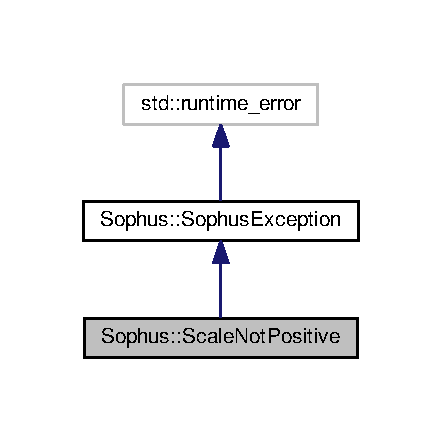
\includegraphics[width=212pt]{class_sophus_1_1_scale_not_positive__inherit__graph}
\end{center}
\end{figure}


Collaboration diagram for Sophus\+:\+:Scale\+Not\+Positive\+:
\nopagebreak
\begin{figure}[H]
\begin{center}
\leavevmode
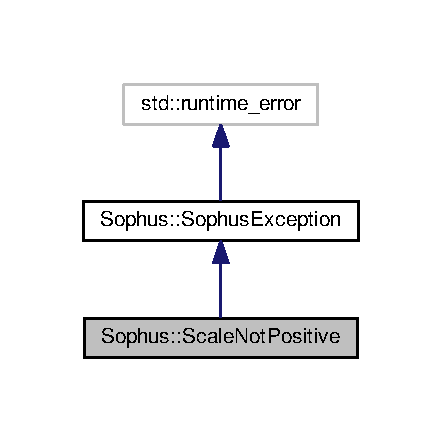
\includegraphics[width=212pt]{class_sophus_1_1_scale_not_positive__coll__graph}
\end{center}
\end{figure}
\subsection*{Additional Inherited Members}


\subsection{Detailed Description}


Definition at line 73 of file rxso3.\+hpp.



The documentation for this class was generated from the following file\+:\begin{DoxyCompactItemize}
\item 
include/\+Sophus/sophus/rxso3.\+hpp\end{DoxyCompactItemize}

\hypertarget{class_sophus_1_1_s_e2_group}{}\section{Sophus\+:\+:S\+E2\+Group$<$ \+\_\+\+Scalar, \+\_\+\+Options $>$ Class Template Reference}
\label{class_sophus_1_1_s_e2_group}\index{Sophus\+::\+S\+E2\+Group$<$ \+\_\+\+Scalar, \+\_\+\+Options $>$@{Sophus\+::\+S\+E2\+Group$<$ \+\_\+\+Scalar, \+\_\+\+Options $>$}}


S\+E2 default type -\/ Constructors and default storage for S\+E2 Type.  




{\ttfamily \#include $<$se2.\+hpp$>$}



Inheritance diagram for Sophus\+:\+:S\+E2\+Group$<$ \+\_\+\+Scalar, \+\_\+\+Options $>$\+:
\nopagebreak
\begin{figure}[H]
\begin{center}
\leavevmode
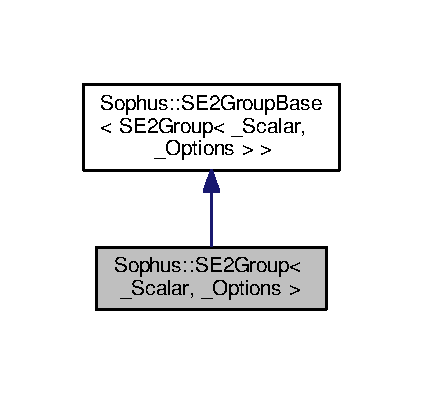
\includegraphics[width=203pt]{class_sophus_1_1_s_e2_group__inherit__graph}
\end{center}
\end{figure}


Collaboration diagram for Sophus\+:\+:S\+E2\+Group$<$ \+\_\+\+Scalar, \+\_\+\+Options $>$\+:
\nopagebreak
\begin{figure}[H]
\begin{center}
\leavevmode
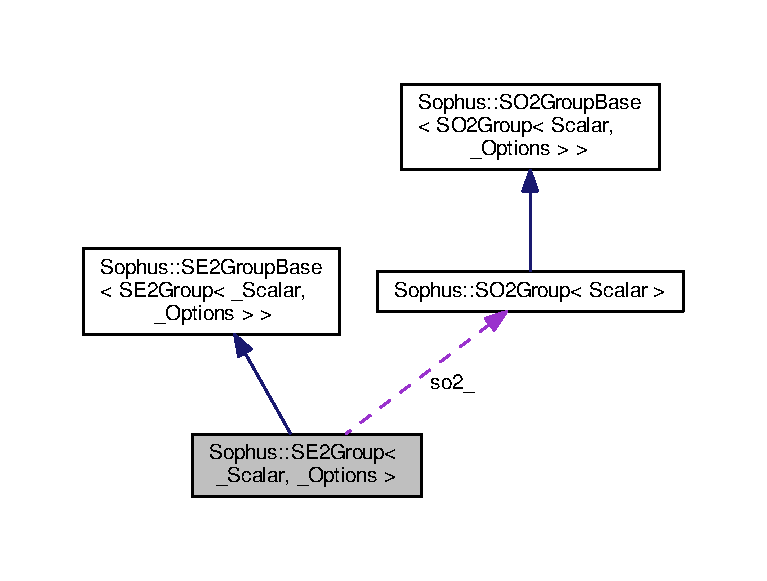
\includegraphics[width=350pt]{class_sophus_1_1_s_e2_group__coll__graph}
\end{center}
\end{figure}
\subsection*{Public Types}
\begin{DoxyCompactItemize}
\item 
typedef internal\+::traits$<$ \hyperlink{class_sophus_1_1_s_e2_group}{S\+E2\+Group}$<$ \+\_\+\+Scalar, \+\_\+\+Options $>$ $>$\+::\hyperlink{class_sophus_1_1_s_e2_group_a2c3f69904c79825984774d78a107ab35}{Scalar} \hyperlink{class_sophus_1_1_s_e2_group_a2c3f69904c79825984774d78a107ab35}{Scalar}\hypertarget{class_sophus_1_1_s_e2_group_a2c3f69904c79825984774d78a107ab35}{}\label{class_sophus_1_1_s_e2_group_a2c3f69904c79825984774d78a107ab35}

\begin{DoxyCompactList}\small\item\em scalar type \end{DoxyCompactList}\item 
typedef internal\+::traits$<$ \hyperlink{class_sophus_1_1_s_e2_group}{S\+E2\+Group}$<$ \+\_\+\+Scalar, \+\_\+\+Options $>$ $>$\+::Translation\+Type \& \hyperlink{class_sophus_1_1_s_e2_group_afa2e2598cfa5844e7d6a57b5c0b6a38a}{Translation\+Reference}\hypertarget{class_sophus_1_1_s_e2_group_afa2e2598cfa5844e7d6a57b5c0b6a38a}{}\label{class_sophus_1_1_s_e2_group_afa2e2598cfa5844e7d6a57b5c0b6a38a}

\begin{DoxyCompactList}\small\item\em translation reference type \end{DoxyCompactList}\item 
typedef const internal\+::traits$<$ \hyperlink{class_sophus_1_1_s_e2_group}{S\+E2\+Group}$<$ \+\_\+\+Scalar, \+\_\+\+Options $>$ $>$\+::Translation\+Type \& {\bfseries Const\+Translation\+Reference}\hypertarget{class_sophus_1_1_s_e2_group_aa74333930e3caebf50564bc2a40a6eff}{}\label{class_sophus_1_1_s_e2_group_aa74333930e3caebf50564bc2a40a6eff}

\item 
typedef internal\+::traits$<$ \hyperlink{class_sophus_1_1_s_e2_group}{S\+E2\+Group}$<$ \+\_\+\+Scalar, \+\_\+\+Options $>$ $>$\+::S\+O2\+Type \& \hyperlink{class_sophus_1_1_s_e2_group_a053aa9fd3ee6259f817472e7e4c46a06}{S\+O2\+Reference}\hypertarget{class_sophus_1_1_s_e2_group_a053aa9fd3ee6259f817472e7e4c46a06}{}\label{class_sophus_1_1_s_e2_group_a053aa9fd3ee6259f817472e7e4c46a06}

\begin{DoxyCompactList}\small\item\em S\+O2 reference type. \end{DoxyCompactList}\item 
typedef const internal\+::traits$<$ \hyperlink{class_sophus_1_1_s_e2_group}{S\+E2\+Group}$<$ \+\_\+\+Scalar, \+\_\+\+Options $>$ $>$\+::S\+O2\+Type \& \hyperlink{class_sophus_1_1_s_e2_group_a370e66451d1133612595dc3fb30e07cf}{Const\+S\+O2\+Reference}\hypertarget{class_sophus_1_1_s_e2_group_a370e66451d1133612595dc3fb30e07cf}{}\label{class_sophus_1_1_s_e2_group_a370e66451d1133612595dc3fb30e07cf}

\begin{DoxyCompactList}\small\item\em S\+O2 const reference type. \end{DoxyCompactList}\item 
typedef \hyperlink{class_sophus_1_1_s_e2_group_base_a82fe531d4b64813525d4ebd131da9bcd}{Base\+::\+Transformation} \hyperlink{class_sophus_1_1_s_e2_group_a53519178925a6384fbffa13451e6011d}{Transformation}\hypertarget{class_sophus_1_1_s_e2_group_a53519178925a6384fbffa13451e6011d}{}\label{class_sophus_1_1_s_e2_group_a53519178925a6384fbffa13451e6011d}

\begin{DoxyCompactList}\small\item\em group transfomation type \end{DoxyCompactList}\item 
typedef \hyperlink{class_sophus_1_1_s_e2_group_base_add8b024098bc6fcecdefb42229fa881b}{Base\+::\+Point} \hyperlink{class_sophus_1_1_s_e2_group_a2c5e73ee0291af22e7cf6194caee546b}{Point}\hypertarget{class_sophus_1_1_s_e2_group_a2c5e73ee0291af22e7cf6194caee546b}{}\label{class_sophus_1_1_s_e2_group_a2c5e73ee0291af22e7cf6194caee546b}

\begin{DoxyCompactList}\small\item\em point type \end{DoxyCompactList}\item 
typedef \hyperlink{class_sophus_1_1_s_e2_group_base_a71b41e6cde48514241c7bffcbe34923f}{Base\+::\+Tangent} \hyperlink{class_sophus_1_1_s_e2_group_a6e7d63930d03ddbd8c29cbb57de288e9}{Tangent}\hypertarget{class_sophus_1_1_s_e2_group_a6e7d63930d03ddbd8c29cbb57de288e9}{}\label{class_sophus_1_1_s_e2_group_a6e7d63930d03ddbd8c29cbb57de288e9}

\begin{DoxyCompactList}\small\item\em tangent vector type \end{DoxyCompactList}\item 
typedef \hyperlink{class_sophus_1_1_s_e2_group_base_a6e0785a6f8399456a8bd0b057bae02ee}{Base\+::\+Adjoint} \hyperlink{class_sophus_1_1_s_e2_group_a1ab5bbc31d258dc1999f221e3013a45c}{Adjoint}\hypertarget{class_sophus_1_1_s_e2_group_a1ab5bbc31d258dc1999f221e3013a45c}{}\label{class_sophus_1_1_s_e2_group_a1ab5bbc31d258dc1999f221e3013a45c}

\begin{DoxyCompactList}\small\item\em adjoint transformation type \end{DoxyCompactList}\end{DoxyCompactItemize}
\subsection*{Public Member Functions}
\begin{DoxyCompactItemize}
\item 
E\+I\+G\+E\+N\+\_\+\+M\+A\+K\+E\+\_\+\+A\+L\+I\+G\+N\+E\+D\+\_\+\+O\+P\+E\+R\+A\+T\+O\+R\+\_\+\+N\+EW \hyperlink{class_sophus_1_1_s_e2_group_acc6ff82594e8782f87206fe56368b843}{S\+E2\+Group} ()
\begin{DoxyCompactList}\small\item\em Default constructor. \end{DoxyCompactList}\item 
{\footnotesize template$<$typename Other\+Derived $>$ }\\\hyperlink{class_sophus_1_1_s_e2_group_ac28c38a52364c13b35294e4bf393c564}{S\+E2\+Group} (const \hyperlink{class_sophus_1_1_s_e2_group_base}{S\+E2\+Group\+Base}$<$ Other\+Derived $>$ \&other)\hypertarget{class_sophus_1_1_s_e2_group_ac28c38a52364c13b35294e4bf393c564}{}\label{class_sophus_1_1_s_e2_group_ac28c38a52364c13b35294e4bf393c564}

\begin{DoxyCompactList}\small\item\em Copy constructor. \end{DoxyCompactList}\item 
{\footnotesize template$<$typename Other\+Derived $>$ }\\\hyperlink{class_sophus_1_1_s_e2_group_aff6488a201f733b1742c81b4e8148c75}{S\+E2\+Group} (const \hyperlink{class_sophus_1_1_s_o2_group_base}{S\+O2\+Group\+Base}$<$ Other\+Derived $>$ \&\hyperlink{class_sophus_1_1_s_e2_group_a6f3c739ac63f076ce266409558ede468}{so2}, const \hyperlink{class_sophus_1_1_s_e2_group_a2c5e73ee0291af22e7cf6194caee546b}{Point} \&\hyperlink{class_sophus_1_1_s_e2_group_a6e63c40c66f69c7b363570a532b90aab}{translation})\hypertarget{class_sophus_1_1_s_e2_group_aff6488a201f733b1742c81b4e8148c75}{}\label{class_sophus_1_1_s_e2_group_aff6488a201f733b1742c81b4e8148c75}

\begin{DoxyCompactList}\small\item\em Constructor from S\+O2 and translation vector. \end{DoxyCompactList}\item 
\hyperlink{class_sophus_1_1_s_e2_group_a515c3ca29d9e8cff0394f93dd891720a}{S\+E2\+Group} (const typename \hyperlink{class_sophus_1_1_s_o2_group}{S\+O2\+Group}$<$ \hyperlink{class_sophus_1_1_s_e2_group_a2c3f69904c79825984774d78a107ab35}{Scalar} $>$\+::\hyperlink{class_sophus_1_1_s_e2_group_a53519178925a6384fbffa13451e6011d}{Transformation} \&rotation\+\_\+matrix, const \hyperlink{class_sophus_1_1_s_e2_group_a2c5e73ee0291af22e7cf6194caee546b}{Point} \&\hyperlink{class_sophus_1_1_s_e2_group_a6e63c40c66f69c7b363570a532b90aab}{translation})
\begin{DoxyCompactList}\small\item\em Constructor from rotation matrix and translation vector. \end{DoxyCompactList}\item 
\hyperlink{class_sophus_1_1_s_e2_group_a4b803331ce9cc6b86768594b4647dd85}{S\+E2\+Group} (const \hyperlink{class_sophus_1_1_s_e2_group_a2c3f69904c79825984774d78a107ab35}{Scalar} \&theta, const \hyperlink{class_sophus_1_1_s_e2_group_a2c5e73ee0291af22e7cf6194caee546b}{Point} \&\hyperlink{class_sophus_1_1_s_e2_group_a6e63c40c66f69c7b363570a532b90aab}{translation})\hypertarget{class_sophus_1_1_s_e2_group_a4b803331ce9cc6b86768594b4647dd85}{}\label{class_sophus_1_1_s_e2_group_a4b803331ce9cc6b86768594b4647dd85}

\begin{DoxyCompactList}\small\item\em Constructor from rotation angle and translation vector. \end{DoxyCompactList}\item 
\hyperlink{class_sophus_1_1_s_e2_group_ae04e1102f0aa8cd87345a777e43533c6}{S\+E2\+Group} (const std\+::complex$<$ \hyperlink{class_sophus_1_1_s_e2_group_a2c3f69904c79825984774d78a107ab35}{Scalar} $>$ \&complex, const \hyperlink{class_sophus_1_1_s_e2_group_a2c5e73ee0291af22e7cf6194caee546b}{Point} \&\hyperlink{class_sophus_1_1_s_e2_group_a6e63c40c66f69c7b363570a532b90aab}{translation})
\begin{DoxyCompactList}\small\item\em Constructor from complex number and translation vector. \end{DoxyCompactList}\item 
\hyperlink{class_sophus_1_1_s_e2_group_ac1f39ff125e3e2be151e9dcb0c555706}{S\+E2\+Group} (const \hyperlink{class_sophus_1_1_s_e2_group_a53519178925a6384fbffa13451e6011d}{Transformation} \&T)
\begin{DoxyCompactList}\small\item\em Constructor from 3x3 matrix. \end{DoxyCompactList}\item 
E\+I\+G\+E\+N\+\_\+\+S\+T\+R\+O\+N\+G\+\_\+\+I\+N\+L\+I\+NE \hyperlink{class_sophus_1_1_s_e2_group_a2c3f69904c79825984774d78a107ab35}{Scalar} $\ast$ \hyperlink{class_sophus_1_1_s_e2_group_a748b0248723a888eb712349027eeb123}{data} ()
\item 
E\+I\+G\+E\+N\+\_\+\+S\+T\+R\+O\+N\+G\+\_\+\+I\+N\+L\+I\+NE const \hyperlink{class_sophus_1_1_s_e2_group_a2c3f69904c79825984774d78a107ab35}{Scalar} $\ast$ \hyperlink{class_sophus_1_1_s_e2_group_a76dbc3478e64eaebce1972ce3eadcf43}{data} () const 
\item 
E\+I\+G\+E\+N\+\_\+\+S\+T\+R\+O\+N\+G\+\_\+\+I\+N\+L\+I\+NE \hyperlink{class_sophus_1_1_s_e2_group_a053aa9fd3ee6259f817472e7e4c46a06}{S\+O2\+Reference} \hyperlink{class_sophus_1_1_s_e2_group_a6f3c739ac63f076ce266409558ede468}{so2} ()\hypertarget{class_sophus_1_1_s_e2_group_a6f3c739ac63f076ce266409558ede468}{}\label{class_sophus_1_1_s_e2_group_a6f3c739ac63f076ce266409558ede468}

\begin{DoxyCompactList}\small\item\em Accessor of S\+O2. \end{DoxyCompactList}\item 
E\+I\+G\+E\+N\+\_\+\+S\+T\+R\+O\+N\+G\+\_\+\+I\+N\+L\+I\+NE \hyperlink{class_sophus_1_1_s_e2_group_a370e66451d1133612595dc3fb30e07cf}{Const\+S\+O2\+Reference} \hyperlink{class_sophus_1_1_s_e2_group_afc84a8f7f21ef10e729160dd20ebf81e}{so2} () const \hypertarget{class_sophus_1_1_s_e2_group_afc84a8f7f21ef10e729160dd20ebf81e}{}\label{class_sophus_1_1_s_e2_group_afc84a8f7f21ef10e729160dd20ebf81e}

\begin{DoxyCompactList}\small\item\em Mutator of S\+O2. \end{DoxyCompactList}\item 
E\+I\+G\+E\+N\+\_\+\+S\+T\+R\+O\+N\+G\+\_\+\+I\+N\+L\+I\+NE \hyperlink{class_sophus_1_1_s_e2_group_afa2e2598cfa5844e7d6a57b5c0b6a38a}{Translation\+Reference} \hyperlink{class_sophus_1_1_s_e2_group_a6e63c40c66f69c7b363570a532b90aab}{translation} ()\hypertarget{class_sophus_1_1_s_e2_group_a6e63c40c66f69c7b363570a532b90aab}{}\label{class_sophus_1_1_s_e2_group_a6e63c40c66f69c7b363570a532b90aab}

\begin{DoxyCompactList}\small\item\em Mutator of translation vector. \end{DoxyCompactList}\item 
E\+I\+G\+E\+N\+\_\+\+S\+T\+R\+O\+N\+G\+\_\+\+I\+N\+L\+I\+NE Const\+Translation\+Reference \hyperlink{class_sophus_1_1_s_e2_group_ae6096a12944c7c6b92b74609a84a6888}{translation} () const \hypertarget{class_sophus_1_1_s_e2_group_ae6096a12944c7c6b92b74609a84a6888}{}\label{class_sophus_1_1_s_e2_group_ae6096a12944c7c6b92b74609a84a6888}

\begin{DoxyCompactList}\small\item\em Accessor of translation vector. \end{DoxyCompactList}\end{DoxyCompactItemize}
\subsection*{Static Public Attributes}
\begin{DoxyCompactItemize}
\item 
static const int \hyperlink{class_sophus_1_1_s_e2_group_a4c578d8a3dd37d860b45db0497759098}{DoF} = Base\+::\+DoF\hypertarget{class_sophus_1_1_s_e2_group_a4c578d8a3dd37d860b45db0497759098}{}\label{class_sophus_1_1_s_e2_group_a4c578d8a3dd37d860b45db0497759098}

\begin{DoxyCompactList}\small\item\em degree of freedom of group \end{DoxyCompactList}\item 
static const int \hyperlink{class_sophus_1_1_s_e2_group_a98c89f88343958bb3c65c1b3240cf295}{num\+\_\+parameters} = Base\+::num\+\_\+parameters\hypertarget{class_sophus_1_1_s_e2_group_a98c89f88343958bb3c65c1b3240cf295}{}\label{class_sophus_1_1_s_e2_group_a98c89f88343958bb3c65c1b3240cf295}

\begin{DoxyCompactList}\small\item\em number of internal parameters used \end{DoxyCompactList}\item 
static const int \hyperlink{class_sophus_1_1_s_e2_group_abbe9d16d13ed2351b7e0589f89e9d502}{N} = Base\+::N\hypertarget{class_sophus_1_1_s_e2_group_abbe9d16d13ed2351b7e0589f89e9d502}{}\label{class_sophus_1_1_s_e2_group_abbe9d16d13ed2351b7e0589f89e9d502}

\begin{DoxyCompactList}\small\item\em group transformations are NxN matrices \end{DoxyCompactList}\end{DoxyCompactItemize}
\subsection*{Protected Attributes}
\begin{DoxyCompactItemize}
\item 
\hyperlink{class_sophus_1_1_s_o2_group}{Sophus\+::\+S\+O2\+Group}$<$ \hyperlink{class_sophus_1_1_s_e2_group_a2c3f69904c79825984774d78a107ab35}{Scalar} $>$ {\bfseries so2\+\_\+}\hypertarget{class_sophus_1_1_s_e2_group_a5e02fb49e86a4a4adb230850ecb9a96a}{}\label{class_sophus_1_1_s_e2_group_a5e02fb49e86a4a4adb230850ecb9a96a}

\item 
Matrix$<$ \hyperlink{class_sophus_1_1_s_e2_group_a2c3f69904c79825984774d78a107ab35}{Scalar}, 2, 1 $>$ {\bfseries translation\+\_\+}\hypertarget{class_sophus_1_1_s_e2_group_ab99e569e0d4765534f595f4243cf0e33}{}\label{class_sophus_1_1_s_e2_group_ab99e569e0d4765534f595f4243cf0e33}

\end{DoxyCompactItemize}
\subsection*{Additional Inherited Members}


\subsection{Detailed Description}
\subsubsection*{template$<$typename \+\_\+\+Scalar, int \+\_\+\+Options$>$\\*
class Sophus\+::\+S\+E2\+Group$<$ \+\_\+\+Scalar, \+\_\+\+Options $>$}

S\+E2 default type -\/ Constructors and default storage for S\+E2 Type. 

Definition at line 33 of file se2.\+hpp.



\subsection{Constructor \& Destructor Documentation}
\index{Sophus\+::\+S\+E2\+Group@{Sophus\+::\+S\+E2\+Group}!S\+E2\+Group@{S\+E2\+Group}}
\index{S\+E2\+Group@{S\+E2\+Group}!Sophus\+::\+S\+E2\+Group@{Sophus\+::\+S\+E2\+Group}}
\subsubsection[{\texorpdfstring{S\+E2\+Group()}{SE2Group()}}]{\setlength{\rightskip}{0pt plus 5cm}template$<$typename \+\_\+\+Scalar, int \+\_\+\+Options$>$ E\+I\+G\+E\+N\+\_\+\+M\+A\+K\+E\+\_\+\+A\+L\+I\+G\+N\+E\+D\+\_\+\+O\+P\+E\+R\+A\+T\+O\+R\+\_\+\+N\+EW {\bf Sophus\+::\+S\+E2\+Group}$<$ \+\_\+\+Scalar, \+\_\+\+Options $>$\+::{\bf S\+E2\+Group} (
\begin{DoxyParamCaption}
{}
\end{DoxyParamCaption}
)\hspace{0.3cm}{\ttfamily [inline]}}\hypertarget{class_sophus_1_1_s_e2_group_acc6ff82594e8782f87206fe56368b843}{}\label{class_sophus_1_1_s_e2_group_acc6ff82594e8782f87206fe56368b843}


Default constructor. 

Initialize Complex to identity rotation and translation to zero. 

Definition at line 611 of file se2.\+hpp.

\index{Sophus\+::\+S\+E2\+Group@{Sophus\+::\+S\+E2\+Group}!S\+E2\+Group@{S\+E2\+Group}}
\index{S\+E2\+Group@{S\+E2\+Group}!Sophus\+::\+S\+E2\+Group@{Sophus\+::\+S\+E2\+Group}}
\subsubsection[{\texorpdfstring{S\+E2\+Group(const typename S\+O2\+Group$<$ Scalar $>$\+::\+Transformation \&rotation\+\_\+matrix, const Point \&translation)}{SE2Group(const typename SO2Group< Scalar >::Transformation &rotation_matrix, const Point &translation)}}]{\setlength{\rightskip}{0pt plus 5cm}template$<$typename \+\_\+\+Scalar, int \+\_\+\+Options$>$ {\bf Sophus\+::\+S\+E2\+Group}$<$ \+\_\+\+Scalar, \+\_\+\+Options $>$\+::{\bf S\+E2\+Group} (
\begin{DoxyParamCaption}
\item[{const typename {\bf S\+O2\+Group}$<$ {\bf Scalar} $>$\+::{\bf Transformation} \&}]{rotation\+\_\+matrix, }
\item[{const {\bf Point} \&}]{translation}
\end{DoxyParamCaption}
)\hspace{0.3cm}{\ttfamily [inline]}}\hypertarget{class_sophus_1_1_s_e2_group_a515c3ca29d9e8cff0394f93dd891720a}{}\label{class_sophus_1_1_s_e2_group_a515c3ca29d9e8cff0394f93dd891720a}


Constructor from rotation matrix and translation vector. 

\begin{DoxyPrecond}{Precondition}
rotation matrix need to be orthogonal with determinant of 1 
\end{DoxyPrecond}


Definition at line 639 of file se2.\+hpp.

\index{Sophus\+::\+S\+E2\+Group@{Sophus\+::\+S\+E2\+Group}!S\+E2\+Group@{S\+E2\+Group}}
\index{S\+E2\+Group@{S\+E2\+Group}!Sophus\+::\+S\+E2\+Group@{Sophus\+::\+S\+E2\+Group}}
\subsubsection[{\texorpdfstring{S\+E2\+Group(const std\+::complex$<$ Scalar $>$ \&complex, const Point \&translation)}{SE2Group(const std::complex< Scalar > &complex, const Point &translation)}}]{\setlength{\rightskip}{0pt plus 5cm}template$<$typename \+\_\+\+Scalar, int \+\_\+\+Options$>$ {\bf Sophus\+::\+S\+E2\+Group}$<$ \+\_\+\+Scalar, \+\_\+\+Options $>$\+::{\bf S\+E2\+Group} (
\begin{DoxyParamCaption}
\item[{const std\+::complex$<$ {\bf Scalar} $>$ \&}]{complex, }
\item[{const {\bf Point} \&}]{translation}
\end{DoxyParamCaption}
)\hspace{0.3cm}{\ttfamily [inline]}}\hypertarget{class_sophus_1_1_s_e2_group_ae04e1102f0aa8cd87345a777e43533c6}{}\label{class_sophus_1_1_s_e2_group_ae04e1102f0aa8cd87345a777e43533c6}


Constructor from complex number and translation vector. 

\begin{DoxyPrecond}{Precondition}
complex must not be zero 
\end{DoxyPrecond}


Definition at line 659 of file se2.\+hpp.

\index{Sophus\+::\+S\+E2\+Group@{Sophus\+::\+S\+E2\+Group}!S\+E2\+Group@{S\+E2\+Group}}
\index{S\+E2\+Group@{S\+E2\+Group}!Sophus\+::\+S\+E2\+Group@{Sophus\+::\+S\+E2\+Group}}
\subsubsection[{\texorpdfstring{S\+E2\+Group(const Transformation \&\+T)}{SE2Group(const Transformation &T)}}]{\setlength{\rightskip}{0pt plus 5cm}template$<$typename \+\_\+\+Scalar, int \+\_\+\+Options$>$ {\bf Sophus\+::\+S\+E2\+Group}$<$ \+\_\+\+Scalar, \+\_\+\+Options $>$\+::{\bf S\+E2\+Group} (
\begin{DoxyParamCaption}
\item[{const {\bf Transformation} \&}]{T}
\end{DoxyParamCaption}
)\hspace{0.3cm}{\ttfamily [inline]}, {\ttfamily [explicit]}}\hypertarget{class_sophus_1_1_s_e2_group_ac1f39ff125e3e2be151e9dcb0c555706}{}\label{class_sophus_1_1_s_e2_group_ac1f39ff125e3e2be151e9dcb0c555706}


Constructor from 3x3 matrix. 

\begin{DoxyPrecond}{Precondition}
2x2 sub-\/matrix need to be orthogonal with determinant of 1 
\end{DoxyPrecond}


Definition at line 670 of file se2.\+hpp.



\subsection{Member Function Documentation}
\index{Sophus\+::\+S\+E2\+Group@{Sophus\+::\+S\+E2\+Group}!data@{data}}
\index{data@{data}!Sophus\+::\+S\+E2\+Group@{Sophus\+::\+S\+E2\+Group}}
\subsubsection[{\texorpdfstring{data()}{data()}}]{\setlength{\rightskip}{0pt plus 5cm}template$<$typename \+\_\+\+Scalar, int \+\_\+\+Options$>$ E\+I\+G\+E\+N\+\_\+\+S\+T\+R\+O\+N\+G\+\_\+\+I\+N\+L\+I\+NE {\bf Scalar}$\ast$ {\bf Sophus\+::\+S\+E2\+Group}$<$ \+\_\+\+Scalar, \+\_\+\+Options $>$\+::data (
\begin{DoxyParamCaption}
{}
\end{DoxyParamCaption}
)\hspace{0.3cm}{\ttfamily [inline]}}\hypertarget{class_sophus_1_1_s_e2_group_a748b0248723a888eb712349027eeb123}{}\label{class_sophus_1_1_s_e2_group_a748b0248723a888eb712349027eeb123}
\begin{DoxyReturn}{Returns}
pointer to internal data
\end{DoxyReturn}
This provides unsafe read/write access to internal data. S\+E2 is represented by a pair of an S\+O2 element (two parameters) and a translation vector (two parameters). The user needs to take care of that the complex stays normalized.

/see \hyperlink{class_sophus_1_1_s_e2_group_base_aa53b166d7053572efeb5b77a08834156}{normalize()} 

Definition at line 686 of file se2.\+hpp.

\index{Sophus\+::\+S\+E2\+Group@{Sophus\+::\+S\+E2\+Group}!data@{data}}
\index{data@{data}!Sophus\+::\+S\+E2\+Group@{Sophus\+::\+S\+E2\+Group}}
\subsubsection[{\texorpdfstring{data() const }{data() const }}]{\setlength{\rightskip}{0pt plus 5cm}template$<$typename \+\_\+\+Scalar, int \+\_\+\+Options$>$ E\+I\+G\+E\+N\+\_\+\+S\+T\+R\+O\+N\+G\+\_\+\+I\+N\+L\+I\+NE const {\bf Scalar}$\ast$ {\bf Sophus\+::\+S\+E2\+Group}$<$ \+\_\+\+Scalar, \+\_\+\+Options $>$\+::data (
\begin{DoxyParamCaption}
{}
\end{DoxyParamCaption}
) const\hspace{0.3cm}{\ttfamily [inline]}}\hypertarget{class_sophus_1_1_s_e2_group_a76dbc3478e64eaebce1972ce3eadcf43}{}\label{class_sophus_1_1_s_e2_group_a76dbc3478e64eaebce1972ce3eadcf43}
\begin{DoxyReturn}{Returns}
const pointer to internal data
\end{DoxyReturn}
Const version of \hyperlink{class_sophus_1_1_s_e2_group_a748b0248723a888eb712349027eeb123}{data()}. 

Definition at line 697 of file se2.\+hpp.



The documentation for this class was generated from the following file\+:\begin{DoxyCompactItemize}
\item 
include/\+Sophus/sophus/se2.\+hpp\end{DoxyCompactItemize}

\hypertarget{class_sophus_1_1_s_e2_group_base}{}\section{Sophus\+:\+:S\+E2\+Group\+Base$<$ Derived $>$ Class Template Reference}
\label{class_sophus_1_1_s_e2_group_base}\index{Sophus\+::\+S\+E2\+Group\+Base$<$ Derived $>$@{Sophus\+::\+S\+E2\+Group\+Base$<$ Derived $>$}}


S\+E2 base type -\/ implements S\+E2 class but is storage agnostic.  




{\ttfamily \#include $<$se2.\+hpp$>$}

\subsection*{Public Types}
\begin{DoxyCompactItemize}
\item 
typedef internal\+::traits$<$ Derived $>$\+::\hyperlink{class_sophus_1_1_s_e2_group_base_a1bad7970c24437df7f4a34281ff147fe}{Scalar} \hyperlink{class_sophus_1_1_s_e2_group_base_a1bad7970c24437df7f4a34281ff147fe}{Scalar}\hypertarget{class_sophus_1_1_s_e2_group_base_a1bad7970c24437df7f4a34281ff147fe}{}\label{class_sophus_1_1_s_e2_group_base_a1bad7970c24437df7f4a34281ff147fe}

\begin{DoxyCompactList}\small\item\em scalar type \end{DoxyCompactList}\item 
typedef internal\+::traits$<$ Derived $>$\+::Translation\+Type \& \hyperlink{class_sophus_1_1_s_e2_group_base_a971b396ee82cd53a8518bd7d6f216102}{Translation\+Reference}\hypertarget{class_sophus_1_1_s_e2_group_base_a971b396ee82cd53a8518bd7d6f216102}{}\label{class_sophus_1_1_s_e2_group_base_a971b396ee82cd53a8518bd7d6f216102}

\begin{DoxyCompactList}\small\item\em translation reference type \end{DoxyCompactList}\item 
typedef const internal\+::traits$<$ Derived $>$\+::Translation\+Type \& \hyperlink{class_sophus_1_1_s_e2_group_base_a5fbd917de2097049af437e580f3163a3}{Const\+Translation\+Reference}\hypertarget{class_sophus_1_1_s_e2_group_base_a5fbd917de2097049af437e580f3163a3}{}\label{class_sophus_1_1_s_e2_group_base_a5fbd917de2097049af437e580f3163a3}

\begin{DoxyCompactList}\small\item\em translation const reference type \end{DoxyCompactList}\item 
typedef internal\+::traits$<$ Derived $>$\+::S\+O2\+Type \& \hyperlink{class_sophus_1_1_s_e2_group_base_a057dc5e957e17fa3357cf1d2ae800c77}{S\+O2\+Reference}\hypertarget{class_sophus_1_1_s_e2_group_base_a057dc5e957e17fa3357cf1d2ae800c77}{}\label{class_sophus_1_1_s_e2_group_base_a057dc5e957e17fa3357cf1d2ae800c77}

\begin{DoxyCompactList}\small\item\em S\+O2 reference type. \end{DoxyCompactList}\item 
typedef const internal\+::traits$<$ Derived $>$\+::S\+O2\+Type \& \hyperlink{class_sophus_1_1_s_e2_group_base_a261f36c0d0c957dc49ca5f586c32e3a2}{Const\+S\+O2\+Reference}\hypertarget{class_sophus_1_1_s_e2_group_base_a261f36c0d0c957dc49ca5f586c32e3a2}{}\label{class_sophus_1_1_s_e2_group_base_a261f36c0d0c957dc49ca5f586c32e3a2}

\begin{DoxyCompactList}\small\item\em S\+O2 type. \end{DoxyCompactList}\item 
typedef Matrix$<$ \hyperlink{class_sophus_1_1_s_e2_group_base_a1bad7970c24437df7f4a34281ff147fe}{Scalar}, \hyperlink{class_sophus_1_1_s_e2_group_base_a07b0f26b806ad9cd07184d817bc462a1}{N}, \hyperlink{class_sophus_1_1_s_e2_group_base_a07b0f26b806ad9cd07184d817bc462a1}{N} $>$ \hyperlink{class_sophus_1_1_s_e2_group_base_a82fe531d4b64813525d4ebd131da9bcd}{Transformation}\hypertarget{class_sophus_1_1_s_e2_group_base_a82fe531d4b64813525d4ebd131da9bcd}{}\label{class_sophus_1_1_s_e2_group_base_a82fe531d4b64813525d4ebd131da9bcd}

\begin{DoxyCompactList}\small\item\em group transfomation type \end{DoxyCompactList}\item 
typedef Matrix$<$ \hyperlink{class_sophus_1_1_s_e2_group_base_a1bad7970c24437df7f4a34281ff147fe}{Scalar}, 2, 1 $>$ \hyperlink{class_sophus_1_1_s_e2_group_base_add8b024098bc6fcecdefb42229fa881b}{Point}\hypertarget{class_sophus_1_1_s_e2_group_base_add8b024098bc6fcecdefb42229fa881b}{}\label{class_sophus_1_1_s_e2_group_base_add8b024098bc6fcecdefb42229fa881b}

\begin{DoxyCompactList}\small\item\em point type \end{DoxyCompactList}\item 
typedef Matrix$<$ \hyperlink{class_sophus_1_1_s_e2_group_base_a1bad7970c24437df7f4a34281ff147fe}{Scalar}, \hyperlink{class_sophus_1_1_s_e2_group_base_ab94ffc7ab0cbd8986e6f2ab35c50dbb1}{DoF}, 1 $>$ \hyperlink{class_sophus_1_1_s_e2_group_base_a71b41e6cde48514241c7bffcbe34923f}{Tangent}\hypertarget{class_sophus_1_1_s_e2_group_base_a71b41e6cde48514241c7bffcbe34923f}{}\label{class_sophus_1_1_s_e2_group_base_a71b41e6cde48514241c7bffcbe34923f}

\begin{DoxyCompactList}\small\item\em tangent vector type \end{DoxyCompactList}\item 
typedef Matrix$<$ \hyperlink{class_sophus_1_1_s_e2_group_base_a1bad7970c24437df7f4a34281ff147fe}{Scalar}, \hyperlink{class_sophus_1_1_s_e2_group_base_ab94ffc7ab0cbd8986e6f2ab35c50dbb1}{DoF}, \hyperlink{class_sophus_1_1_s_e2_group_base_ab94ffc7ab0cbd8986e6f2ab35c50dbb1}{DoF} $>$ \hyperlink{class_sophus_1_1_s_e2_group_base_a6e0785a6f8399456a8bd0b057bae02ee}{Adjoint}\hypertarget{class_sophus_1_1_s_e2_group_base_a6e0785a6f8399456a8bd0b057bae02ee}{}\label{class_sophus_1_1_s_e2_group_base_a6e0785a6f8399456a8bd0b057bae02ee}

\begin{DoxyCompactList}\small\item\em adjoint transformation type \end{DoxyCompactList}\end{DoxyCompactItemize}
\subsection*{Public Member Functions}
\begin{DoxyCompactItemize}
\item 
const \hyperlink{class_sophus_1_1_s_e2_group_base_a6e0785a6f8399456a8bd0b057bae02ee}{Adjoint} \hyperlink{class_sophus_1_1_s_e2_group_base_a83dd17e9837363469bbe32ec202cebe5}{Adj} () const 
\begin{DoxyCompactList}\small\item\em Adjoint transformation. \end{DoxyCompactList}\item 
{\footnotesize template$<$typename New\+Scalar\+Type $>$ }\\\hyperlink{class_sophus_1_1_s_e2_group}{S\+E2\+Group}$<$ New\+Scalar\+Type $>$ \hyperlink{class_sophus_1_1_s_e2_group_base_a84e3ce985f4afb7982c2739e2284a276}{cast} () const 
\item 
void \hyperlink{class_sophus_1_1_s_e2_group_base_a51db3eccd7b70627974e9e0f4ba0e0b1}{fast\+Multiply} (const \hyperlink{class_sophus_1_1_s_e2_group}{S\+E2\+Group}$<$ \hyperlink{class_sophus_1_1_s_e2_group_base_a1bad7970c24437df7f4a34281ff147fe}{Scalar} $>$ \&other)
\begin{DoxyCompactList}\small\item\em Fast group multiplication. \end{DoxyCompactList}\item 
const \hyperlink{class_sophus_1_1_s_e2_group}{S\+E2\+Group}$<$ \hyperlink{class_sophus_1_1_s_e2_group_base_a1bad7970c24437df7f4a34281ff147fe}{Scalar} $>$ \hyperlink{class_sophus_1_1_s_e2_group_base_a5c9d9485f696396266bd7932d38d7c90}{inverse} () const 
\item 
const \hyperlink{class_sophus_1_1_s_e2_group_base_a71b41e6cde48514241c7bffcbe34923f}{Tangent} \hyperlink{class_sophus_1_1_s_e2_group_base_a32855c8b44ed62a108281a99b7589007}{log} () const 
\begin{DoxyCompactList}\small\item\em Logarithmic map. \end{DoxyCompactList}\item 
void \hyperlink{class_sophus_1_1_s_e2_group_base_aa53b166d7053572efeb5b77a08834156}{normalize} ()
\begin{DoxyCompactList}\small\item\em Normalize S\+O2 element. \end{DoxyCompactList}\item 
const \hyperlink{class_sophus_1_1_s_e2_group_base_a82fe531d4b64813525d4ebd131da9bcd}{Transformation} \hyperlink{class_sophus_1_1_s_e2_group_base_a3d752d2ffd35f2e7eec1466fa451e774}{matrix} () const 
\item 
const Matrix$<$ \hyperlink{class_sophus_1_1_s_e2_group_base_a1bad7970c24437df7f4a34281ff147fe}{Scalar}, 2, 3 $>$ \hyperlink{class_sophus_1_1_s_e2_group_base_a9b312701ec4194c2db4febb83b90c828}{matrix2x3} () const 
\item 
{\footnotesize template$<$typename Other\+Derived $>$ }\\\hyperlink{class_sophus_1_1_s_e2_group_base}{S\+E2\+Group\+Base}$<$ Derived $>$ \& \hyperlink{class_sophus_1_1_s_e2_group_base_abd50c1bef40dc37ac2bc3b707d74d3fc}{operator=} (const \hyperlink{class_sophus_1_1_s_e2_group_base}{S\+E2\+Group\+Base}$<$ Other\+Derived $>$ \&other)\hypertarget{class_sophus_1_1_s_e2_group_base_abd50c1bef40dc37ac2bc3b707d74d3fc}{}\label{class_sophus_1_1_s_e2_group_base_abd50c1bef40dc37ac2bc3b707d74d3fc}

\begin{DoxyCompactList}\small\item\em Assignment operator. \end{DoxyCompactList}\item 
const \hyperlink{class_sophus_1_1_s_e2_group}{S\+E2\+Group}$<$ \hyperlink{class_sophus_1_1_s_e2_group_base_a1bad7970c24437df7f4a34281ff147fe}{Scalar} $>$ \hyperlink{class_sophus_1_1_s_e2_group_base_a36f68c8a9630eed4405f1b89210d421e}{operator$\ast$} (const \hyperlink{class_sophus_1_1_s_e2_group}{S\+E2\+Group}$<$ \hyperlink{class_sophus_1_1_s_e2_group_base_a1bad7970c24437df7f4a34281ff147fe}{Scalar} $>$ \&other) const 
\begin{DoxyCompactList}\small\item\em Group multiplication. \end{DoxyCompactList}\item 
const \hyperlink{class_sophus_1_1_s_e2_group_base_add8b024098bc6fcecdefb42229fa881b}{Point} \hyperlink{class_sophus_1_1_s_e2_group_base_aa1313016f17d4ed280446ad3fef35fff}{operator$\ast$} (const \hyperlink{class_sophus_1_1_s_e2_group_base_add8b024098bc6fcecdefb42229fa881b}{Point} \&p) const 
\begin{DoxyCompactList}\small\item\em Group action on $ \mathbf{R}^2 $. \end{DoxyCompactList}\item 
void \hyperlink{class_sophus_1_1_s_e2_group_base_a5016208d6f5b02464cb4553984e37f29}{operator$\ast$=} (const \hyperlink{class_sophus_1_1_s_e2_group}{S\+E2\+Group}$<$ \hyperlink{class_sophus_1_1_s_e2_group_base_a1bad7970c24437df7f4a34281ff147fe}{Scalar} $>$ \&other)
\begin{DoxyCompactList}\small\item\em In-\/place group multiplication. \end{DoxyCompactList}\item 
const Matrix$<$ \hyperlink{class_sophus_1_1_s_e2_group_base_a1bad7970c24437df7f4a34281ff147fe}{Scalar}, 2, 2 $>$ \hyperlink{class_sophus_1_1_s_e2_group_base_ae70df20893171b2b96a98fae351d1916}{rotation\+Matrix} () const 
\item 
void \hyperlink{class_sophus_1_1_s_e2_group_base_a643d4629d8331be7492b3db74b2bb084}{set\+Complex} (const Matrix$<$ \hyperlink{class_sophus_1_1_s_e2_group_base_a1bad7970c24437df7f4a34281ff147fe}{Scalar}, 2, 1 $>$ \&complex)
\begin{DoxyCompactList}\small\item\em Setter of internal unit complex number representation. \end{DoxyCompactList}\item 
void \hyperlink{class_sophus_1_1_s_e2_group_base_a1d428f01714ff3e3f3df348913645c9b}{set\+Rotation\+Matrix} (const Matrix$<$ \hyperlink{class_sophus_1_1_s_e2_group_base_a1bad7970c24437df7f4a34281ff147fe}{Scalar}, 2, 2 $>$ \&R)
\begin{DoxyCompactList}\small\item\em Setter of unit complex number using rotation matrix. \end{DoxyCompactList}\item 
E\+I\+G\+E\+N\+\_\+\+S\+T\+R\+O\+N\+G\+\_\+\+I\+N\+L\+I\+NE \hyperlink{class_sophus_1_1_s_e2_group_base_a057dc5e957e17fa3357cf1d2ae800c77}{S\+O2\+Reference} \hyperlink{class_sophus_1_1_s_e2_group_base_a7c687ab374c54c578857e3ed03d64e94}{so2} ()\hypertarget{class_sophus_1_1_s_e2_group_base_a7c687ab374c54c578857e3ed03d64e94}{}\label{class_sophus_1_1_s_e2_group_base_a7c687ab374c54c578857e3ed03d64e94}

\begin{DoxyCompactList}\small\item\em Mutator of S\+O2 group. \end{DoxyCompactList}\item 
E\+I\+G\+E\+N\+\_\+\+S\+T\+R\+O\+N\+G\+\_\+\+I\+N\+L\+I\+NE \hyperlink{class_sophus_1_1_s_e2_group_base_a261f36c0d0c957dc49ca5f586c32e3a2}{Const\+S\+O2\+Reference} \hyperlink{class_sophus_1_1_s_e2_group_base_ac644101eacda42115dfb3fecd5bc5eca}{so2} () const \hypertarget{class_sophus_1_1_s_e2_group_base_ac644101eacda42115dfb3fecd5bc5eca}{}\label{class_sophus_1_1_s_e2_group_base_ac644101eacda42115dfb3fecd5bc5eca}

\begin{DoxyCompactList}\small\item\em Accessor of S\+O2 group. \end{DoxyCompactList}\item 
E\+I\+G\+E\+N\+\_\+\+S\+T\+R\+O\+N\+G\+\_\+\+I\+N\+L\+I\+NE \hyperlink{class_sophus_1_1_s_e2_group_base_a971b396ee82cd53a8518bd7d6f216102}{Translation\+Reference} \hyperlink{class_sophus_1_1_s_e2_group_base_aebf12d78f613797ebfbefdd475ca0c6d}{translation} ()\hypertarget{class_sophus_1_1_s_e2_group_base_aebf12d78f613797ebfbefdd475ca0c6d}{}\label{class_sophus_1_1_s_e2_group_base_aebf12d78f613797ebfbefdd475ca0c6d}

\begin{DoxyCompactList}\small\item\em Mutator of translation vector. \end{DoxyCompactList}\item 
E\+I\+G\+E\+N\+\_\+\+S\+T\+R\+O\+N\+G\+\_\+\+I\+N\+L\+I\+NE \hyperlink{class_sophus_1_1_s_e2_group_base_a5fbd917de2097049af437e580f3163a3}{Const\+Translation\+Reference} \hyperlink{class_sophus_1_1_s_e2_group_base_a5a17942302897237f35657a7133fe8de}{translation} () const \hypertarget{class_sophus_1_1_s_e2_group_base_a5a17942302897237f35657a7133fe8de}{}\label{class_sophus_1_1_s_e2_group_base_a5a17942302897237f35657a7133fe8de}

\begin{DoxyCompactList}\small\item\em Accessor of translation vector. \end{DoxyCompactList}\item 
internal\+::traits$<$ Derived $>$\+::S\+O2\+Type\+::\+Const\+Complex\+Reference \hyperlink{class_sophus_1_1_s_e2_group_base_ace841824d980bbe39f28241df52d646c}{unit\+\_\+complex} () const 
\begin{DoxyCompactList}\small\item\em Accessor of unit complex number. \end{DoxyCompactList}\end{DoxyCompactItemize}
\subsection*{Static Public Member Functions}
\begin{DoxyCompactItemize}
\item 
static const \hyperlink{class_sophus_1_1_s_e2_group_base_a82fe531d4b64813525d4ebd131da9bcd}{Transformation} \hyperlink{class_sophus_1_1_s_e2_group_base_abd82580529a773695f83e6768c865c5c}{d\+\_\+lie\+Bracketab\+\_\+by\+\_\+d\+\_\+a} (const \hyperlink{class_sophus_1_1_s_e2_group_base_a71b41e6cde48514241c7bffcbe34923f}{Tangent} \&b)
\item 
static const \hyperlink{class_sophus_1_1_s_e2_group}{S\+E2\+Group}$<$ \hyperlink{class_sophus_1_1_s_e2_group_base_a1bad7970c24437df7f4a34281ff147fe}{Scalar} $>$ \hyperlink{class_sophus_1_1_s_e2_group_base_ade77e270e09a1719b56e765ee7c8967f}{exp} (const \hyperlink{class_sophus_1_1_s_e2_group_base_a71b41e6cde48514241c7bffcbe34923f}{Tangent} \&a)
\begin{DoxyCompactList}\small\item\em Group exponential. \end{DoxyCompactList}\item 
static const \hyperlink{class_sophus_1_1_s_e2_group_base_a82fe531d4b64813525d4ebd131da9bcd}{Transformation} \hyperlink{class_sophus_1_1_s_e2_group_base_a3d255ebf6a3101e2e79ae3dd97af6cbc}{generator} (int i)
\begin{DoxyCompactList}\small\item\em Generators. \end{DoxyCompactList}\item 
static const \hyperlink{class_sophus_1_1_s_e2_group_base_a82fe531d4b64813525d4ebd131da9bcd}{Transformation} \hyperlink{class_sophus_1_1_s_e2_group_base_aa5d381596ee614e1b32a36515c67287a}{hat} (const \hyperlink{class_sophus_1_1_s_e2_group_base_a71b41e6cde48514241c7bffcbe34923f}{Tangent} \&v)
\begin{DoxyCompactList}\small\item\em hat-\/operator \end{DoxyCompactList}\item 
static const \hyperlink{class_sophus_1_1_s_e2_group_base_a71b41e6cde48514241c7bffcbe34923f}{Tangent} \hyperlink{class_sophus_1_1_s_e2_group_base_ab3de14df064c6d609d1f3855edc065a8}{lie\+Bracket} (const \hyperlink{class_sophus_1_1_s_e2_group_base_a71b41e6cde48514241c7bffcbe34923f}{Tangent} \&a, const \hyperlink{class_sophus_1_1_s_e2_group_base_a71b41e6cde48514241c7bffcbe34923f}{Tangent} \&b)
\begin{DoxyCompactList}\small\item\em Lie bracket. \end{DoxyCompactList}\item 
static const \hyperlink{class_sophus_1_1_s_e2_group_base_a71b41e6cde48514241c7bffcbe34923f}{Tangent} \hyperlink{class_sophus_1_1_s_e2_group_base_aecc7909b366aa35b033f6c704441ac70}{log} (const \hyperlink{class_sophus_1_1_s_e2_group}{S\+E2\+Group}$<$ \hyperlink{class_sophus_1_1_s_e2_group_base_a1bad7970c24437df7f4a34281ff147fe}{Scalar} $>$ \&other)
\begin{DoxyCompactList}\small\item\em Logarithmic map. \end{DoxyCompactList}\item 
static const \hyperlink{class_sophus_1_1_s_e2_group_base_a71b41e6cde48514241c7bffcbe34923f}{Tangent} \hyperlink{class_sophus_1_1_s_e2_group_base_a7d4d4cab49ee63e2e2592f3637cdac34}{vee} (const \hyperlink{class_sophus_1_1_s_e2_group_base_a82fe531d4b64813525d4ebd131da9bcd}{Transformation} \&Omega)
\begin{DoxyCompactList}\small\item\em vee-\/operator \end{DoxyCompactList}\end{DoxyCompactItemize}
\subsection*{Static Public Attributes}
\begin{DoxyCompactItemize}
\item 
static const int \hyperlink{class_sophus_1_1_s_e2_group_base_ab94ffc7ab0cbd8986e6f2ab35c50dbb1}{DoF} = 3\hypertarget{class_sophus_1_1_s_e2_group_base_ab94ffc7ab0cbd8986e6f2ab35c50dbb1}{}\label{class_sophus_1_1_s_e2_group_base_ab94ffc7ab0cbd8986e6f2ab35c50dbb1}

\begin{DoxyCompactList}\small\item\em degree of freedom of group (two for translation, one for in-\/plane rotation) \end{DoxyCompactList}\item 
static const int \hyperlink{class_sophus_1_1_s_e2_group_base_a304bd88bbf7f60bb7f8982d84fdb9653}{num\+\_\+parameters} = 4\hypertarget{class_sophus_1_1_s_e2_group_base_a304bd88bbf7f60bb7f8982d84fdb9653}{}\label{class_sophus_1_1_s_e2_group_base_a304bd88bbf7f60bb7f8982d84fdb9653}

\begin{DoxyCompactList}\small\item\em number of internal parameters used (unit complex number for rotation + translation 2-\/vector) \end{DoxyCompactList}\item 
static const int \hyperlink{class_sophus_1_1_s_e2_group_base_a07b0f26b806ad9cd07184d817bc462a1}{N} = 3\hypertarget{class_sophus_1_1_s_e2_group_base_a07b0f26b806ad9cd07184d817bc462a1}{}\label{class_sophus_1_1_s_e2_group_base_a07b0f26b806ad9cd07184d817bc462a1}

\begin{DoxyCompactList}\small\item\em group transformations are NxN matrices \end{DoxyCompactList}\end{DoxyCompactItemize}


\subsection{Detailed Description}
\subsubsection*{template$<$typename Derived$>$\\*
class Sophus\+::\+S\+E2\+Group\+Base$<$ Derived $>$}

S\+E2 base type -\/ implements S\+E2 class but is storage agnostic. 

\mbox{[}add more detailed description/tutorial\mbox{]} 

Definition at line 82 of file se2.\+hpp.



\subsection{Member Function Documentation}
\index{Sophus\+::\+S\+E2\+Group\+Base@{Sophus\+::\+S\+E2\+Group\+Base}!Adj@{Adj}}
\index{Adj@{Adj}!Sophus\+::\+S\+E2\+Group\+Base@{Sophus\+::\+S\+E2\+Group\+Base}}
\subsubsection[{\texorpdfstring{Adj() const }{Adj() const }}]{\setlength{\rightskip}{0pt plus 5cm}template$<$typename Derived$>$ const {\bf Adjoint} {\bf Sophus\+::\+S\+E2\+Group\+Base}$<$ Derived $>$\+::Adj (
\begin{DoxyParamCaption}
{}
\end{DoxyParamCaption}
) const\hspace{0.3cm}{\ttfamily [inline]}}\hypertarget{class_sophus_1_1_s_e2_group_base_a83dd17e9837363469bbe32ec202cebe5}{}\label{class_sophus_1_1_s_e2_group_base_a83dd17e9837363469bbe32ec202cebe5}


Adjoint transformation. 

This function return the adjoint transformation $ Ad $ of the group instance $ A $ such that for all $ x $ it holds that $ \widehat{Ad_A\cdot x} = A\widehat{x}A^{-1} $ with $\ \widehat{\cdot} $ being the \hyperlink{class_sophus_1_1_s_e2_group_base_aa5d381596ee614e1b32a36515c67287a}{hat()}-\/operator. 

Definition at line 125 of file se2.\+hpp.

\index{Sophus\+::\+S\+E2\+Group\+Base@{Sophus\+::\+S\+E2\+Group\+Base}!cast@{cast}}
\index{cast@{cast}!Sophus\+::\+S\+E2\+Group\+Base@{Sophus\+::\+S\+E2\+Group\+Base}}
\subsubsection[{\texorpdfstring{cast() const }{cast() const }}]{\setlength{\rightskip}{0pt plus 5cm}template$<$typename Derived$>$ template$<$typename New\+Scalar\+Type $>$ {\bf S\+E2\+Group}$<$New\+Scalar\+Type$>$ {\bf Sophus\+::\+S\+E2\+Group\+Base}$<$ Derived $>$\+::cast (
\begin{DoxyParamCaption}
{}
\end{DoxyParamCaption}
) const\hspace{0.3cm}{\ttfamily [inline]}}\hypertarget{class_sophus_1_1_s_e2_group_base_a84e3ce985f4afb7982c2739e2284a276}{}\label{class_sophus_1_1_s_e2_group_base_a84e3ce985f4afb7982c2739e2284a276}
\begin{DoxyReturn}{Returns}
copy of instance casted to New\+Scalar\+Type 
\end{DoxyReturn}


Definition at line 139 of file se2.\+hpp.

\index{Sophus\+::\+S\+E2\+Group\+Base@{Sophus\+::\+S\+E2\+Group\+Base}!d\+\_\+lie\+Bracketab\+\_\+by\+\_\+d\+\_\+a@{d\+\_\+lie\+Bracketab\+\_\+by\+\_\+d\+\_\+a}}
\index{d\+\_\+lie\+Bracketab\+\_\+by\+\_\+d\+\_\+a@{d\+\_\+lie\+Bracketab\+\_\+by\+\_\+d\+\_\+a}!Sophus\+::\+S\+E2\+Group\+Base@{Sophus\+::\+S\+E2\+Group\+Base}}
\subsubsection[{\texorpdfstring{d\+\_\+lie\+Bracketab\+\_\+by\+\_\+d\+\_\+a(const Tangent \&b)}{d_lieBracketab_by_d_a(const Tangent &b)}}]{\setlength{\rightskip}{0pt plus 5cm}template$<$typename Derived$>$ static const {\bf Transformation} {\bf Sophus\+::\+S\+E2\+Group\+Base}$<$ Derived $>$\+::d\+\_\+lie\+Bracketab\+\_\+by\+\_\+d\+\_\+a (
\begin{DoxyParamCaption}
\item[{const {\bf Tangent} \&}]{b}
\end{DoxyParamCaption}
)\hspace{0.3cm}{\ttfamily [inline]}, {\ttfamily [static]}}\hypertarget{class_sophus_1_1_s_e2_group_base_abd82580529a773695f83e6768c865c5c}{}\label{class_sophus_1_1_s_e2_group_base_abd82580529a773695f83e6768c865c5c}

\begin{DoxyParams}{Parameters}
{\em b} & 3-\/vector representation of Lie algebra element \\
\hline
\end{DoxyParams}
\begin{DoxyReturn}{Returns}
derivative of Lie bracket
\end{DoxyReturn}
This function returns $ \frac{\partial}{\partial a} [a, b]_{se2} $ with $ [a, b]_{se2} $ being the \hyperlink{class_sophus_1_1_s_e2_group_base_ab3de14df064c6d609d1f3855edc065a8}{lie\+Bracket()} of the Lie algebra se2.

\begin{DoxySeeAlso}{See also}
\hyperlink{class_sophus_1_1_s_e2_group_base_ab3de14df064c6d609d1f3855edc065a8}{lie\+Bracket()} 
\end{DoxySeeAlso}


Definition at line 359 of file se2.\+hpp.

\index{Sophus\+::\+S\+E2\+Group\+Base@{Sophus\+::\+S\+E2\+Group\+Base}!exp@{exp}}
\index{exp@{exp}!Sophus\+::\+S\+E2\+Group\+Base@{Sophus\+::\+S\+E2\+Group\+Base}}
\subsubsection[{\texorpdfstring{exp(const Tangent \&a)}{exp(const Tangent &a)}}]{\setlength{\rightskip}{0pt plus 5cm}template$<$typename Derived$>$ static const {\bf S\+E2\+Group}$<${\bf Scalar}$>$ {\bf Sophus\+::\+S\+E2\+Group\+Base}$<$ Derived $>$\+::exp (
\begin{DoxyParamCaption}
\item[{const {\bf Tangent} \&}]{a}
\end{DoxyParamCaption}
)\hspace{0.3cm}{\ttfamily [inline]}, {\ttfamily [static]}}\hypertarget{class_sophus_1_1_s_e2_group_base_ade77e270e09a1719b56e765ee7c8967f}{}\label{class_sophus_1_1_s_e2_group_base_ade77e270e09a1719b56e765ee7c8967f}


Group exponential. 


\begin{DoxyParams}{Parameters}
{\em a} & tangent space element (3-\/vector) \\
\hline
\end{DoxyParams}
\begin{DoxyReturn}{Returns}
corresponding element of the group S\+E2
\end{DoxyReturn}
The first two components of $ a $ represent the translational part $ \upsilon $ in the tangent space of S\+E2, while the last components of $ a $ is the rotation angle $ \theta $.

To be more specific, this function computes $ \exp(\widehat{a}) $ with $ \exp(\cdot) $ being the matrix exponential and $ \widehat{\cdot} $ the \hyperlink{class_sophus_1_1_s_e2_group_base_aa5d381596ee614e1b32a36515c67287a}{hat()}-\/operator of S\+E2.

\begin{DoxySeeAlso}{See also}
\hyperlink{class_sophus_1_1_s_e2_group_base_aa5d381596ee614e1b32a36515c67287a}{hat()} 

\hyperlink{class_sophus_1_1_s_e2_group_base_a32855c8b44ed62a108281a99b7589007}{log()} 
\end{DoxySeeAlso}


Definition at line 389 of file se2.\+hpp.

\index{Sophus\+::\+S\+E2\+Group\+Base@{Sophus\+::\+S\+E2\+Group\+Base}!fast\+Multiply@{fast\+Multiply}}
\index{fast\+Multiply@{fast\+Multiply}!Sophus\+::\+S\+E2\+Group\+Base@{Sophus\+::\+S\+E2\+Group\+Base}}
\subsubsection[{\texorpdfstring{fast\+Multiply(const S\+E2\+Group$<$ Scalar $>$ \&other)}{fastMultiply(const SE2Group< Scalar > &other)}}]{\setlength{\rightskip}{0pt plus 5cm}template$<$typename Derived$>$ void {\bf Sophus\+::\+S\+E2\+Group\+Base}$<$ Derived $>$\+::fast\+Multiply (
\begin{DoxyParamCaption}
\item[{const {\bf S\+E2\+Group}$<$ {\bf Scalar} $>$ \&}]{other}
\end{DoxyParamCaption}
)\hspace{0.3cm}{\ttfamily [inline]}}\hypertarget{class_sophus_1_1_s_e2_group_base_a51db3eccd7b70627974e9e0f4ba0e0b1}{}\label{class_sophus_1_1_s_e2_group_base_a51db3eccd7b70627974e9e0f4ba0e0b1}


Fast group multiplication. 

This method is a fast version of \hyperlink{class_sophus_1_1_s_e2_group_base_a5016208d6f5b02464cb4553984e37f29}{operator$\ast$=()}, since it does not perform normalization. It is up to the user to call \hyperlink{class_sophus_1_1_s_e2_group_base_aa53b166d7053572efeb5b77a08834156}{normalize()} once in a while.

\begin{DoxySeeAlso}{See also}
\hyperlink{class_sophus_1_1_s_e2_group_base_a5016208d6f5b02464cb4553984e37f29}{operator$\ast$=()} 
\end{DoxySeeAlso}


Definition at line 154 of file se2.\+hpp.

\index{Sophus\+::\+S\+E2\+Group\+Base@{Sophus\+::\+S\+E2\+Group\+Base}!generator@{generator}}
\index{generator@{generator}!Sophus\+::\+S\+E2\+Group\+Base@{Sophus\+::\+S\+E2\+Group\+Base}}
\subsubsection[{\texorpdfstring{generator(int i)}{generator(int i)}}]{\setlength{\rightskip}{0pt plus 5cm}template$<$typename Derived$>$ static const {\bf Transformation} {\bf Sophus\+::\+S\+E2\+Group\+Base}$<$ Derived $>$\+::generator (
\begin{DoxyParamCaption}
\item[{int}]{i}
\end{DoxyParamCaption}
)\hspace{0.3cm}{\ttfamily [inline]}, {\ttfamily [static]}}\hypertarget{class_sophus_1_1_s_e2_group_base_a3d255ebf6a3101e2e79ae3dd97af6cbc}{}\label{class_sophus_1_1_s_e2_group_base_a3d255ebf6a3101e2e79ae3dd97af6cbc}


Generators. 

\begin{DoxyPrecond}{Precondition}
$ i \in \{0,1,2\} $ 
\end{DoxyPrecond}
\begin{DoxyReturn}{Returns}
$ i $th generator $ G_i $ of S\+E2
\end{DoxyReturn}
The infinitesimal generators of S\+E2 are\+: \[ G_0 = \left( \begin{array}{ccc} 0& 0& 1\\ 0& 0& 0\\ 0& 0& 0\\ \end{array} \right), G_1 = \left( \begin{array}{cccc} 0& 0& 0\\ 0& 0& 1\\ 0& 0& 0\\ \end{array} \right), G_2 = \left( \begin{array}{cccc} 0& 0& 0&\\ 0& 0& -1&\\ 0& 1& 0&\\ \end{array} \right), \] \begin{DoxySeeAlso}{See also}
\hyperlink{class_sophus_1_1_s_e2_group_base_aa5d381596ee614e1b32a36515c67287a}{hat()} 
\end{DoxySeeAlso}


Definition at line 439 of file se2.\+hpp.

\index{Sophus\+::\+S\+E2\+Group\+Base@{Sophus\+::\+S\+E2\+Group\+Base}!hat@{hat}}
\index{hat@{hat}!Sophus\+::\+S\+E2\+Group\+Base@{Sophus\+::\+S\+E2\+Group\+Base}}
\subsubsection[{\texorpdfstring{hat(const Tangent \&v)}{hat(const Tangent &v)}}]{\setlength{\rightskip}{0pt plus 5cm}template$<$typename Derived$>$ static const {\bf Transformation} {\bf Sophus\+::\+S\+E2\+Group\+Base}$<$ Derived $>$\+::hat (
\begin{DoxyParamCaption}
\item[{const {\bf Tangent} \&}]{v}
\end{DoxyParamCaption}
)\hspace{0.3cm}{\ttfamily [inline]}, {\ttfamily [static]}}\hypertarget{class_sophus_1_1_s_e2_group_base_aa5d381596ee614e1b32a36515c67287a}{}\label{class_sophus_1_1_s_e2_group_base_aa5d381596ee614e1b32a36515c67287a}


hat-\/operator 


\begin{DoxyParams}{Parameters}
{\em omega} & 3-\/vector representation of Lie algebra element \\
\hline
\end{DoxyParams}
\begin{DoxyReturn}{Returns}
3x3-\/matrix representatin of Lie algebra element
\end{DoxyReturn}
Formally, the hat-\/operator of S\+E2 is defined as $ \widehat{\cdot}: \mathbf{R}^3 \rightarrow \mathbf{R}^{2\times 2}, \quad \widehat{\omega} = \sum_{i=0}^2 G_i \omega_i $ with $ G_i $ being the ith infinitesial \hyperlink{class_sophus_1_1_s_e2_group_base_a3d255ebf6a3101e2e79ae3dd97af6cbc}{generator()}.

\begin{DoxySeeAlso}{See also}
\hyperlink{class_sophus_1_1_s_e2_group_base_a3d255ebf6a3101e2e79ae3dd97af6cbc}{generator()} 

\hyperlink{class_sophus_1_1_s_e2_group_base_a7d4d4cab49ee63e2e2592f3637cdac34}{vee()} 
\end{DoxySeeAlso}


Definition at line 464 of file se2.\+hpp.

\index{Sophus\+::\+S\+E2\+Group\+Base@{Sophus\+::\+S\+E2\+Group\+Base}!inverse@{inverse}}
\index{inverse@{inverse}!Sophus\+::\+S\+E2\+Group\+Base@{Sophus\+::\+S\+E2\+Group\+Base}}
\subsubsection[{\texorpdfstring{inverse() const }{inverse() const }}]{\setlength{\rightskip}{0pt plus 5cm}template$<$typename Derived$>$ const {\bf S\+E2\+Group}$<${\bf Scalar}$>$ {\bf Sophus\+::\+S\+E2\+Group\+Base}$<$ Derived $>$\+::inverse (
\begin{DoxyParamCaption}
{}
\end{DoxyParamCaption}
) const\hspace{0.3cm}{\ttfamily [inline]}}\hypertarget{class_sophus_1_1_s_e2_group_base_a5c9d9485f696396266bd7932d38d7c90}{}\label{class_sophus_1_1_s_e2_group_base_a5c9d9485f696396266bd7932d38d7c90}
\begin{DoxyReturn}{Returns}
Group inverse of instance 
\end{DoxyReturn}


Definition at line 163 of file se2.\+hpp.

\index{Sophus\+::\+S\+E2\+Group\+Base@{Sophus\+::\+S\+E2\+Group\+Base}!lie\+Bracket@{lie\+Bracket}}
\index{lie\+Bracket@{lie\+Bracket}!Sophus\+::\+S\+E2\+Group\+Base@{Sophus\+::\+S\+E2\+Group\+Base}}
\subsubsection[{\texorpdfstring{lie\+Bracket(const Tangent \&a, const Tangent \&b)}{lieBracket(const Tangent &a, const Tangent &b)}}]{\setlength{\rightskip}{0pt plus 5cm}template$<$typename Derived$>$ static const {\bf Tangent} {\bf Sophus\+::\+S\+E2\+Group\+Base}$<$ Derived $>$\+::lie\+Bracket (
\begin{DoxyParamCaption}
\item[{const {\bf Tangent} \&}]{a, }
\item[{const {\bf Tangent} \&}]{b}
\end{DoxyParamCaption}
)\hspace{0.3cm}{\ttfamily [inline]}, {\ttfamily [static]}}\hypertarget{class_sophus_1_1_s_e2_group_base_ab3de14df064c6d609d1f3855edc065a8}{}\label{class_sophus_1_1_s_e2_group_base_ab3de14df064c6d609d1f3855edc065a8}


Lie bracket. 


\begin{DoxyParams}{Parameters}
{\em a} & 3-\/vector representation of Lie algebra element \\
\hline
{\em b} & 3-\/vector representation of Lie algebra element \\
\hline
\end{DoxyParams}
\begin{DoxyReturn}{Returns}
3-\/vector representation of Lie algebra element
\end{DoxyReturn}
It computes the bracket of S\+E2. To be more specific, it computes $ [a, b]_{se2} := [\widehat{a_1}, \widehat{b_2}]^\vee $ with $ [A,B] = AB-BA $ being the matrix commutator, $ \widehat{\cdot} $ the \hyperlink{class_sophus_1_1_s_e2_group_base_aa5d381596ee614e1b32a36515c67287a}{hat()}-\/operator and $ (\cdot)^\vee $ the \hyperlink{class_sophus_1_1_s_e2_group_base_a7d4d4cab49ee63e2e2592f3637cdac34}{vee()}-\/operator of S\+E2.

\begin{DoxySeeAlso}{See also}
\hyperlink{class_sophus_1_1_s_e2_group_base_aa5d381596ee614e1b32a36515c67287a}{hat()} 

\hyperlink{class_sophus_1_1_s_e2_group_base_a7d4d4cab49ee63e2e2592f3637cdac34}{vee()} 
\end{DoxySeeAlso}


Definition at line 490 of file se2.\+hpp.

\index{Sophus\+::\+S\+E2\+Group\+Base@{Sophus\+::\+S\+E2\+Group\+Base}!log@{log}}
\index{log@{log}!Sophus\+::\+S\+E2\+Group\+Base@{Sophus\+::\+S\+E2\+Group\+Base}}
\subsubsection[{\texorpdfstring{log() const }{log() const }}]{\setlength{\rightskip}{0pt plus 5cm}template$<$typename Derived$>$ const {\bf Tangent} {\bf Sophus\+::\+S\+E2\+Group\+Base}$<$ Derived $>$\+::log (
\begin{DoxyParamCaption}
{}
\end{DoxyParamCaption}
) const\hspace{0.3cm}{\ttfamily [inline]}}\hypertarget{class_sophus_1_1_s_e2_group_base_a32855c8b44ed62a108281a99b7589007}{}\label{class_sophus_1_1_s_e2_group_base_a32855c8b44ed62a108281a99b7589007}


Logarithmic map. 

\begin{DoxyReturn}{Returns}
tangent space representation (translational part and rotation angle) of instance
\end{DoxyReturn}
\begin{DoxySeeAlso}{See also}
\hyperlink{class_sophus_1_1_s_e2_group_base_a32855c8b44ed62a108281a99b7589007}{log()}. 
\end{DoxySeeAlso}


Definition at line 178 of file se2.\+hpp.

\index{Sophus\+::\+S\+E2\+Group\+Base@{Sophus\+::\+S\+E2\+Group\+Base}!log@{log}}
\index{log@{log}!Sophus\+::\+S\+E2\+Group\+Base@{Sophus\+::\+S\+E2\+Group\+Base}}
\subsubsection[{\texorpdfstring{log(const S\+E2\+Group$<$ Scalar $>$ \&other)}{log(const SE2Group< Scalar > &other)}}]{\setlength{\rightskip}{0pt plus 5cm}template$<$typename Derived$>$ static const {\bf Tangent} {\bf Sophus\+::\+S\+E2\+Group\+Base}$<$ Derived $>$\+::log (
\begin{DoxyParamCaption}
\item[{const {\bf S\+E2\+Group}$<$ {\bf Scalar} $>$ \&}]{other}
\end{DoxyParamCaption}
)\hspace{0.3cm}{\ttfamily [inline]}, {\ttfamily [static]}}\hypertarget{class_sophus_1_1_s_e2_group_base_aecc7909b366aa35b033f6c704441ac70}{}\label{class_sophus_1_1_s_e2_group_base_aecc7909b366aa35b033f6c704441ac70}


Logarithmic map. 


\begin{DoxyParams}{Parameters}
{\em other} & element of the group S\+E2 \\
\hline
\end{DoxyParams}
\begin{DoxyReturn}{Returns}
corresponding tangent space element (translational part $ \upsilon $ and rotation vector $ \omega $)
\end{DoxyReturn}
Computes the logarithmic, the inverse of the group exponential. To be specific, this function computes $ \log({\cdot})^\vee $ with $ \vee(\cdot) $ being the matrix logarithm and $ \vee{\cdot} $ the \hyperlink{class_sophus_1_1_s_e2_group_base_a7d4d4cab49ee63e2e2592f3637cdac34}{vee()}-\/operator of S\+E2.

\begin{DoxySeeAlso}{See also}
\hyperlink{class_sophus_1_1_s_e2_group_base_ade77e270e09a1719b56e765ee7c8967f}{exp()} 

\hyperlink{class_sophus_1_1_s_e2_group_base_a7d4d4cab49ee63e2e2592f3637cdac34}{vee()} 
\end{DoxySeeAlso}


Definition at line 519 of file se2.\+hpp.

\index{Sophus\+::\+S\+E2\+Group\+Base@{Sophus\+::\+S\+E2\+Group\+Base}!matrix@{matrix}}
\index{matrix@{matrix}!Sophus\+::\+S\+E2\+Group\+Base@{Sophus\+::\+S\+E2\+Group\+Base}}
\subsubsection[{\texorpdfstring{matrix() const }{matrix() const }}]{\setlength{\rightskip}{0pt plus 5cm}template$<$typename Derived$>$ const {\bf Transformation} {\bf Sophus\+::\+S\+E2\+Group\+Base}$<$ Derived $>$\+::matrix (
\begin{DoxyParamCaption}
{}
\end{DoxyParamCaption}
) const\hspace{0.3cm}{\ttfamily [inline]}}\hypertarget{class_sophus_1_1_s_e2_group_base_a3d752d2ffd35f2e7eec1466fa451e774}{}\label{class_sophus_1_1_s_e2_group_base_a3d752d2ffd35f2e7eec1466fa451e774}
\begin{DoxyReturn}{Returns}
3x3 matrix representation of instance 
\end{DoxyReturn}


Definition at line 197 of file se2.\+hpp.

\index{Sophus\+::\+S\+E2\+Group\+Base@{Sophus\+::\+S\+E2\+Group\+Base}!matrix2x3@{matrix2x3}}
\index{matrix2x3@{matrix2x3}!Sophus\+::\+S\+E2\+Group\+Base@{Sophus\+::\+S\+E2\+Group\+Base}}
\subsubsection[{\texorpdfstring{matrix2x3() const }{matrix2x3() const }}]{\setlength{\rightskip}{0pt plus 5cm}template$<$typename Derived$>$ const Matrix$<${\bf Scalar},2,3$>$ {\bf Sophus\+::\+S\+E2\+Group\+Base}$<$ Derived $>$\+::matrix2x3 (
\begin{DoxyParamCaption}
{}
\end{DoxyParamCaption}
) const\hspace{0.3cm}{\ttfamily [inline]}}\hypertarget{class_sophus_1_1_s_e2_group_base_a9b312701ec4194c2db4febb83b90c828}{}\label{class_sophus_1_1_s_e2_group_base_a9b312701ec4194c2db4febb83b90c828}
\begin{DoxyReturn}{Returns}
2x3 matrix representation of instance
\end{DoxyReturn}
It returns the three first row of \hyperlink{class_sophus_1_1_s_e2_group_base_a3d752d2ffd35f2e7eec1466fa451e774}{matrix()}. 

Definition at line 211 of file se2.\+hpp.

\index{Sophus\+::\+S\+E2\+Group\+Base@{Sophus\+::\+S\+E2\+Group\+Base}!normalize@{normalize}}
\index{normalize@{normalize}!Sophus\+::\+S\+E2\+Group\+Base@{Sophus\+::\+S\+E2\+Group\+Base}}
\subsubsection[{\texorpdfstring{normalize()}{normalize()}}]{\setlength{\rightskip}{0pt plus 5cm}template$<$typename Derived$>$ void {\bf Sophus\+::\+S\+E2\+Group\+Base}$<$ Derived $>$\+::normalize (
\begin{DoxyParamCaption}
{}
\end{DoxyParamCaption}
)\hspace{0.3cm}{\ttfamily [inline]}}\hypertarget{class_sophus_1_1_s_e2_group_base_aa53b166d7053572efeb5b77a08834156}{}\label{class_sophus_1_1_s_e2_group_base_aa53b166d7053572efeb5b77a08834156}


Normalize S\+O2 element. 

It re-\/normalizes the S\+O2 element. This method only needs to be called in conjunction with \hyperlink{class_sophus_1_1_s_e2_group_base_a51db3eccd7b70627974e9e0f4ba0e0b1}{fast\+Multiply()} or data() write access. 

Definition at line 189 of file se2.\+hpp.

\index{Sophus\+::\+S\+E2\+Group\+Base@{Sophus\+::\+S\+E2\+Group\+Base}!operator$\ast$@{operator$\ast$}}
\index{operator$\ast$@{operator$\ast$}!Sophus\+::\+S\+E2\+Group\+Base@{Sophus\+::\+S\+E2\+Group\+Base}}
\subsubsection[{\texorpdfstring{operator$\ast$(const S\+E2\+Group$<$ Scalar $>$ \&other) const }{operator*(const SE2Group< Scalar > &other) const }}]{\setlength{\rightskip}{0pt plus 5cm}template$<$typename Derived$>$ const {\bf S\+E2\+Group}$<${\bf Scalar}$>$ {\bf Sophus\+::\+S\+E2\+Group\+Base}$<$ Derived $>$\+::operator$\ast$ (
\begin{DoxyParamCaption}
\item[{const {\bf S\+E2\+Group}$<$ {\bf Scalar} $>$ \&}]{other}
\end{DoxyParamCaption}
) const\hspace{0.3cm}{\ttfamily [inline]}}\hypertarget{class_sophus_1_1_s_e2_group_base_a36f68c8a9630eed4405f1b89210d421e}{}\label{class_sophus_1_1_s_e2_group_base_a36f68c8a9630eed4405f1b89210d421e}


Group multiplication. 

\begin{DoxySeeAlso}{See also}
\hyperlink{class_sophus_1_1_s_e2_group_base_a5016208d6f5b02464cb4553984e37f29}{operator$\ast$=()} 
\end{DoxySeeAlso}


Definition at line 233 of file se2.\+hpp.

\index{Sophus\+::\+S\+E2\+Group\+Base@{Sophus\+::\+S\+E2\+Group\+Base}!operator$\ast$@{operator$\ast$}}
\index{operator$\ast$@{operator$\ast$}!Sophus\+::\+S\+E2\+Group\+Base@{Sophus\+::\+S\+E2\+Group\+Base}}
\subsubsection[{\texorpdfstring{operator$\ast$(const Point \&p) const }{operator*(const Point &p) const }}]{\setlength{\rightskip}{0pt plus 5cm}template$<$typename Derived$>$ const {\bf Point} {\bf Sophus\+::\+S\+E2\+Group\+Base}$<$ Derived $>$\+::operator$\ast$ (
\begin{DoxyParamCaption}
\item[{const {\bf Point} \&}]{p}
\end{DoxyParamCaption}
) const\hspace{0.3cm}{\ttfamily [inline]}}\hypertarget{class_sophus_1_1_s_e2_group_base_aa1313016f17d4ed280446ad3fef35fff}{}\label{class_sophus_1_1_s_e2_group_base_aa1313016f17d4ed280446ad3fef35fff}


Group action on $ \mathbf{R}^2 $. 


\begin{DoxyParams}{Parameters}
{\em p} & point $p \in \mathbf{R}^2 $ \\
\hline
\end{DoxyParams}
\begin{DoxyReturn}{Returns}
point $p' \in \mathbf{R}^2 $, rotated and translated version of $p$
\end{DoxyReturn}
This function rotates and translates point $ p $ in $ \mathbf{R}^2 $ by the S\+E2 transformation $R,t$ (=rotation matrix, translation vector)\+: $ p' = R\cdot p + t $. 

Definition at line 251 of file se2.\+hpp.

\index{Sophus\+::\+S\+E2\+Group\+Base@{Sophus\+::\+S\+E2\+Group\+Base}!operator$\ast$=@{operator$\ast$=}}
\index{operator$\ast$=@{operator$\ast$=}!Sophus\+::\+S\+E2\+Group\+Base@{Sophus\+::\+S\+E2\+Group\+Base}}
\subsubsection[{\texorpdfstring{operator$\ast$=(const S\+E2\+Group$<$ Scalar $>$ \&other)}{operator*=(const SE2Group< Scalar > &other)}}]{\setlength{\rightskip}{0pt plus 5cm}template$<$typename Derived$>$ void {\bf Sophus\+::\+S\+E2\+Group\+Base}$<$ Derived $>$\+::operator$\ast$= (
\begin{DoxyParamCaption}
\item[{const {\bf S\+E2\+Group}$<$ {\bf Scalar} $>$ \&}]{other}
\end{DoxyParamCaption}
)\hspace{0.3cm}{\ttfamily [inline]}}\hypertarget{class_sophus_1_1_s_e2_group_base_a5016208d6f5b02464cb4553984e37f29}{}\label{class_sophus_1_1_s_e2_group_base_a5016208d6f5b02464cb4553984e37f29}


In-\/place group multiplication. 

\begin{DoxySeeAlso}{See also}
\hyperlink{class_sophus_1_1_s_e2_group_base_a51db3eccd7b70627974e9e0f4ba0e0b1}{fast\+Multiply()} 

\hyperlink{class_sophus_1_1_s_e2_group_base_a36f68c8a9630eed4405f1b89210d421e}{operator$\ast$()} 
\end{DoxySeeAlso}


Definition at line 262 of file se2.\+hpp.

\index{Sophus\+::\+S\+E2\+Group\+Base@{Sophus\+::\+S\+E2\+Group\+Base}!rotation\+Matrix@{rotation\+Matrix}}
\index{rotation\+Matrix@{rotation\+Matrix}!Sophus\+::\+S\+E2\+Group\+Base@{Sophus\+::\+S\+E2\+Group\+Base}}
\subsubsection[{\texorpdfstring{rotation\+Matrix() const }{rotationMatrix() const }}]{\setlength{\rightskip}{0pt plus 5cm}template$<$typename Derived$>$ const Matrix$<${\bf Scalar},2,2$>$ {\bf Sophus\+::\+S\+E2\+Group\+Base}$<$ Derived $>$\+::rotation\+Matrix (
\begin{DoxyParamCaption}
{}
\end{DoxyParamCaption}
) const\hspace{0.3cm}{\ttfamily [inline]}}\hypertarget{class_sophus_1_1_s_e2_group_base_ae70df20893171b2b96a98fae351d1916}{}\label{class_sophus_1_1_s_e2_group_base_ae70df20893171b2b96a98fae351d1916}
\begin{DoxyReturn}{Returns}
Rotation matrix 
\end{DoxyReturn}


Definition at line 272 of file se2.\+hpp.

\index{Sophus\+::\+S\+E2\+Group\+Base@{Sophus\+::\+S\+E2\+Group\+Base}!set\+Complex@{set\+Complex}}
\index{set\+Complex@{set\+Complex}!Sophus\+::\+S\+E2\+Group\+Base@{Sophus\+::\+S\+E2\+Group\+Base}}
\subsubsection[{\texorpdfstring{set\+Complex(const Matrix$<$ Scalar, 2, 1 $>$ \&complex)}{setComplex(const Matrix< Scalar, 2, 1 > &complex)}}]{\setlength{\rightskip}{0pt plus 5cm}template$<$typename Derived$>$ void {\bf Sophus\+::\+S\+E2\+Group\+Base}$<$ Derived $>$\+::set\+Complex (
\begin{DoxyParamCaption}
\item[{const Matrix$<$ {\bf Scalar}, 2, 1 $>$ \&}]{complex}
\end{DoxyParamCaption}
)\hspace{0.3cm}{\ttfamily [inline]}}\hypertarget{class_sophus_1_1_s_e2_group_base_a643d4629d8331be7492b3db74b2bb084}{}\label{class_sophus_1_1_s_e2_group_base_a643d4629d8331be7492b3db74b2bb084}


Setter of internal unit complex number representation. 


\begin{DoxyParams}{Parameters}
{\em complex} & \\
\hline
\end{DoxyParams}
\begin{DoxyPrecond}{Precondition}
the complex number must not be zero
\end{DoxyPrecond}
The complex number is normalized to unit length. 

Definition at line 285 of file se2.\+hpp.

\index{Sophus\+::\+S\+E2\+Group\+Base@{Sophus\+::\+S\+E2\+Group\+Base}!set\+Rotation\+Matrix@{set\+Rotation\+Matrix}}
\index{set\+Rotation\+Matrix@{set\+Rotation\+Matrix}!Sophus\+::\+S\+E2\+Group\+Base@{Sophus\+::\+S\+E2\+Group\+Base}}
\subsubsection[{\texorpdfstring{set\+Rotation\+Matrix(const Matrix$<$ Scalar, 2, 2 $>$ \&\+R)}{setRotationMatrix(const Matrix< Scalar, 2, 2 > &R)}}]{\setlength{\rightskip}{0pt plus 5cm}template$<$typename Derived$>$ void {\bf Sophus\+::\+S\+E2\+Group\+Base}$<$ Derived $>$\+::set\+Rotation\+Matrix (
\begin{DoxyParamCaption}
\item[{const Matrix$<$ {\bf Scalar}, 2, 2 $>$ \&}]{R}
\end{DoxyParamCaption}
)\hspace{0.3cm}{\ttfamily [inline]}}\hypertarget{class_sophus_1_1_s_e2_group_base_a1d428f01714ff3e3f3df348913645c9b}{}\label{class_sophus_1_1_s_e2_group_base_a1d428f01714ff3e3f3df348913645c9b}


Setter of unit complex number using rotation matrix. 


\begin{DoxyParams}{Parameters}
{\em R} & a 2x2 matrix \\
\hline
\end{DoxyParams}
\begin{DoxyPrecond}{Precondition}
the 2x2 matrix should be orthogonal and have a determinant of 1 
\end{DoxyPrecond}


Definition at line 296 of file se2.\+hpp.

\index{Sophus\+::\+S\+E2\+Group\+Base@{Sophus\+::\+S\+E2\+Group\+Base}!unit\+\_\+complex@{unit\+\_\+complex}}
\index{unit\+\_\+complex@{unit\+\_\+complex}!Sophus\+::\+S\+E2\+Group\+Base@{Sophus\+::\+S\+E2\+Group\+Base}}
\subsubsection[{\texorpdfstring{unit\+\_\+complex() const }{unit_complex() const }}]{\setlength{\rightskip}{0pt plus 5cm}template$<$typename Derived$>$ internal\+::traits$<$Derived$>$\+::S\+O2\+Type\+::\+Const\+Complex\+Reference {\bf Sophus\+::\+S\+E2\+Group\+Base}$<$ Derived $>$\+::unit\+\_\+complex (
\begin{DoxyParamCaption}
{}
\end{DoxyParamCaption}
) const\hspace{0.3cm}{\ttfamily [inline]}}\hypertarget{class_sophus_1_1_s_e2_group_base_ace841824d980bbe39f28241df52d646c}{}\label{class_sophus_1_1_s_e2_group_base_ace841824d980bbe39f28241df52d646c}


Accessor of unit complex number. 

No direct write access is given to ensure the complex number stays normalized. 

Definition at line 341 of file se2.\+hpp.

\index{Sophus\+::\+S\+E2\+Group\+Base@{Sophus\+::\+S\+E2\+Group\+Base}!vee@{vee}}
\index{vee@{vee}!Sophus\+::\+S\+E2\+Group\+Base@{Sophus\+::\+S\+E2\+Group\+Base}}
\subsubsection[{\texorpdfstring{vee(const Transformation \&\+Omega)}{vee(const Transformation &Omega)}}]{\setlength{\rightskip}{0pt plus 5cm}template$<$typename Derived$>$ static const {\bf Tangent} {\bf Sophus\+::\+S\+E2\+Group\+Base}$<$ Derived $>$\+::vee (
\begin{DoxyParamCaption}
\item[{const {\bf Transformation} \&}]{Omega}
\end{DoxyParamCaption}
)\hspace{0.3cm}{\ttfamily [inline]}, {\ttfamily [static]}}\hypertarget{class_sophus_1_1_s_e2_group_base_a7d4d4cab49ee63e2e2592f3637cdac34}{}\label{class_sophus_1_1_s_e2_group_base_a7d4d4cab49ee63e2e2592f3637cdac34}


vee-\/operator 


\begin{DoxyParams}{Parameters}
{\em Omega} & 3x3-\/matrix representation of Lie algebra element \\
\hline
\end{DoxyParams}
\begin{DoxyReturn}{Returns}
3-\/vector representatin of Lie algebra element
\end{DoxyReturn}
This is the inverse of the \hyperlink{class_sophus_1_1_s_e2_group_base_aa5d381596ee614e1b32a36515c67287a}{hat()}-\/operator.

\begin{DoxySeeAlso}{See also}
\hyperlink{class_sophus_1_1_s_e2_group_base_aa5d381596ee614e1b32a36515c67287a}{hat()} 
\end{DoxySeeAlso}


Definition at line 555 of file se2.\+hpp.



The documentation for this class was generated from the following file\+:\begin{DoxyCompactItemize}
\item 
include/\+Sophus/sophus/se2.\+hpp\end{DoxyCompactItemize}

\hypertarget{class_sophus_1_1_s_e3_group}{}\section{Sophus\+:\+:S\+E3\+Group$<$ \+\_\+\+Scalar, \+\_\+\+Options $>$ Class Template Reference}
\label{class_sophus_1_1_s_e3_group}\index{Sophus\+::\+S\+E3\+Group$<$ \+\_\+\+Scalar, \+\_\+\+Options $>$@{Sophus\+::\+S\+E3\+Group$<$ \+\_\+\+Scalar, \+\_\+\+Options $>$}}


S\+E3 default type -\/ Constructors and default storage for S\+E3 Type.  




{\ttfamily \#include $<$se3.\+hpp$>$}



Inheritance diagram for Sophus\+:\+:S\+E3\+Group$<$ \+\_\+\+Scalar, \+\_\+\+Options $>$\+:
\nopagebreak
\begin{figure}[H]
\begin{center}
\leavevmode
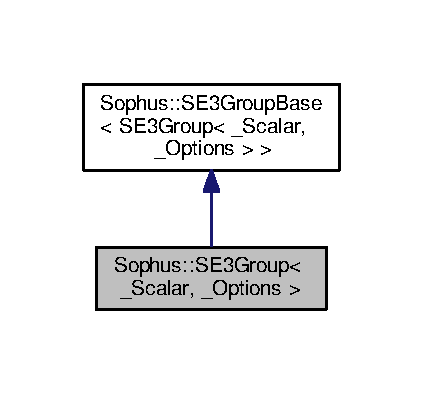
\includegraphics[width=203pt]{class_sophus_1_1_s_e3_group__inherit__graph}
\end{center}
\end{figure}


Collaboration diagram for Sophus\+:\+:S\+E3\+Group$<$ \+\_\+\+Scalar, \+\_\+\+Options $>$\+:
\nopagebreak
\begin{figure}[H]
\begin{center}
\leavevmode
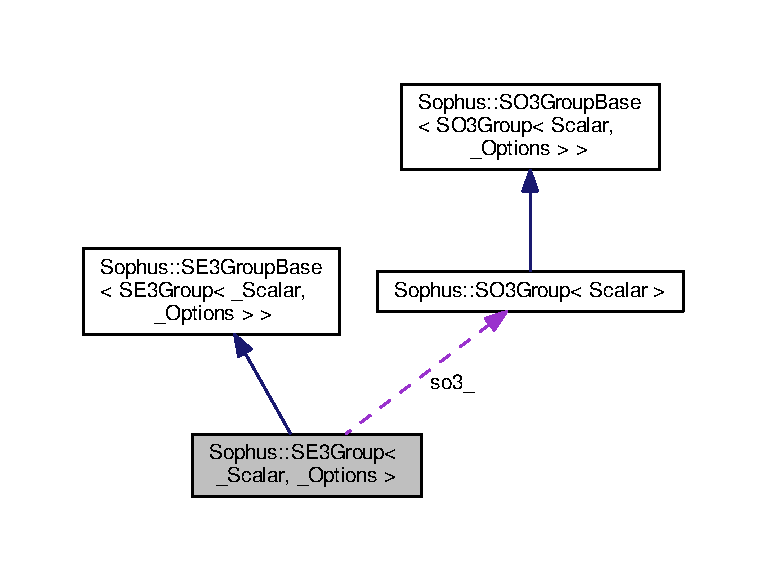
\includegraphics[width=350pt]{class_sophus_1_1_s_e3_group__coll__graph}
\end{center}
\end{figure}
\subsection*{Public Types}
\begin{DoxyCompactItemize}
\item 
typedef internal\+::traits$<$ \hyperlink{class_sophus_1_1_s_e3_group}{S\+E3\+Group}$<$ \+\_\+\+Scalar, \+\_\+\+Options $>$ $>$\+::\hyperlink{class_sophus_1_1_s_e3_group_a8b19ef5ffe83465341b619047581219e}{Scalar} \hyperlink{class_sophus_1_1_s_e3_group_a8b19ef5ffe83465341b619047581219e}{Scalar}\hypertarget{class_sophus_1_1_s_e3_group_a8b19ef5ffe83465341b619047581219e}{}\label{class_sophus_1_1_s_e3_group_a8b19ef5ffe83465341b619047581219e}

\begin{DoxyCompactList}\small\item\em scalar type \end{DoxyCompactList}\item 
typedef internal\+::traits$<$ \hyperlink{class_sophus_1_1_s_e3_group}{S\+E3\+Group}$<$ \+\_\+\+Scalar, \+\_\+\+Options $>$ $>$\+::S\+O3\+Type \& \hyperlink{class_sophus_1_1_s_e3_group_ab9e4d2988d5437bca541db659c76e1a1}{S\+O3\+Reference}\hypertarget{class_sophus_1_1_s_e3_group_ab9e4d2988d5437bca541db659c76e1a1}{}\label{class_sophus_1_1_s_e3_group_ab9e4d2988d5437bca541db659c76e1a1}

\begin{DoxyCompactList}\small\item\em S\+O3 reference type. \end{DoxyCompactList}\item 
typedef const internal\+::traits$<$ \hyperlink{class_sophus_1_1_s_e3_group}{S\+E3\+Group}$<$ \+\_\+\+Scalar, \+\_\+\+Options $>$ $>$\+::S\+O3\+Type \& \hyperlink{class_sophus_1_1_s_e3_group_a448cfe0c4de4a21fe0993472dfc4b981}{Const\+S\+O3\+Reference}\hypertarget{class_sophus_1_1_s_e3_group_a448cfe0c4de4a21fe0993472dfc4b981}{}\label{class_sophus_1_1_s_e3_group_a448cfe0c4de4a21fe0993472dfc4b981}

\begin{DoxyCompactList}\small\item\em S\+O3 const reference type. \end{DoxyCompactList}\item 
typedef internal\+::traits$<$ \hyperlink{class_sophus_1_1_s_e3_group}{S\+E3\+Group}$<$ \+\_\+\+Scalar, \+\_\+\+Options $>$ $>$\+::Translation\+Type \& \hyperlink{class_sophus_1_1_s_e3_group_aecdd5e06df99e50282dbef24632ec622}{Translation\+Reference}\hypertarget{class_sophus_1_1_s_e3_group_aecdd5e06df99e50282dbef24632ec622}{}\label{class_sophus_1_1_s_e3_group_aecdd5e06df99e50282dbef24632ec622}

\begin{DoxyCompactList}\small\item\em translation reference type \end{DoxyCompactList}\item 
typedef const internal\+::traits$<$ \hyperlink{class_sophus_1_1_s_e3_group}{S\+E3\+Group}$<$ \+\_\+\+Scalar, \+\_\+\+Options $>$ $>$\+::Translation\+Type \& \hyperlink{class_sophus_1_1_s_e3_group_a285d764bd862286f24c8fcde6063b30f}{Const\+Translation\+Reference}\hypertarget{class_sophus_1_1_s_e3_group_a285d764bd862286f24c8fcde6063b30f}{}\label{class_sophus_1_1_s_e3_group_a285d764bd862286f24c8fcde6063b30f}

\begin{DoxyCompactList}\small\item\em translation const reference type \end{DoxyCompactList}\item 
typedef \hyperlink{class_sophus_1_1_s_e3_group_base_a426ebd53f324a4fd6d36c28028f967f1}{Base\+::\+Transformation} \hyperlink{class_sophus_1_1_s_e3_group_a1e2ab900cbb05a8740f6174c57ad0861}{Transformation}\hypertarget{class_sophus_1_1_s_e3_group_a1e2ab900cbb05a8740f6174c57ad0861}{}\label{class_sophus_1_1_s_e3_group_a1e2ab900cbb05a8740f6174c57ad0861}

\begin{DoxyCompactList}\small\item\em group transfomation type \end{DoxyCompactList}\item 
typedef \hyperlink{class_sophus_1_1_s_e3_group_base_aca2cf20e857567b74fb399c7ee76c744}{Base\+::\+Point} \hyperlink{class_sophus_1_1_s_e3_group_ab2257f9298559ef83bbeffd386a50e1d}{Point}\hypertarget{class_sophus_1_1_s_e3_group_ab2257f9298559ef83bbeffd386a50e1d}{}\label{class_sophus_1_1_s_e3_group_ab2257f9298559ef83bbeffd386a50e1d}

\begin{DoxyCompactList}\small\item\em point type \end{DoxyCompactList}\item 
typedef \hyperlink{class_sophus_1_1_s_e3_group_base_a45f63b562f0614853cef2c04c4cd5f2b}{Base\+::\+Tangent} \hyperlink{class_sophus_1_1_s_e3_group_a9c2c8a80c34481adfd749d9e0375f56d}{Tangent}\hypertarget{class_sophus_1_1_s_e3_group_a9c2c8a80c34481adfd749d9e0375f56d}{}\label{class_sophus_1_1_s_e3_group_a9c2c8a80c34481adfd749d9e0375f56d}

\begin{DoxyCompactList}\small\item\em tangent vector type \end{DoxyCompactList}\item 
typedef \hyperlink{class_sophus_1_1_s_e3_group_base_ac2e0179cb3e9490604c417d8e59a92d3}{Base\+::\+Adjoint} \hyperlink{class_sophus_1_1_s_e3_group_a4408133c044df81f3d59397874894a6c}{Adjoint}\hypertarget{class_sophus_1_1_s_e3_group_a4408133c044df81f3d59397874894a6c}{}\label{class_sophus_1_1_s_e3_group_a4408133c044df81f3d59397874894a6c}

\begin{DoxyCompactList}\small\item\em adjoint transformation type \end{DoxyCompactList}\end{DoxyCompactItemize}
\subsection*{Public Member Functions}
\begin{DoxyCompactItemize}
\item 
E\+I\+G\+E\+N\+\_\+\+M\+A\+K\+E\+\_\+\+A\+L\+I\+G\+N\+E\+D\+\_\+\+O\+P\+E\+R\+A\+T\+O\+R\+\_\+\+N\+EW \hyperlink{class_sophus_1_1_s_e3_group_a80bb686e6bac8f4cc61b77997b0a6f14}{S\+E3\+Group} ()
\begin{DoxyCompactList}\small\item\em Default constructor. \end{DoxyCompactList}\item 
{\footnotesize template$<$typename Other\+Derived $>$ }\\\hyperlink{class_sophus_1_1_s_e3_group_a5d0436f003940eb003e7c4c2e93b0fbb}{S\+E3\+Group} (const \hyperlink{class_sophus_1_1_s_e3_group_base}{S\+E3\+Group\+Base}$<$ Other\+Derived $>$ \&other)\hypertarget{class_sophus_1_1_s_e3_group_a5d0436f003940eb003e7c4c2e93b0fbb}{}\label{class_sophus_1_1_s_e3_group_a5d0436f003940eb003e7c4c2e93b0fbb}

\begin{DoxyCompactList}\small\item\em Copy constructor. \end{DoxyCompactList}\item 
{\footnotesize template$<$typename Other\+Derived $>$ }\\\hyperlink{class_sophus_1_1_s_e3_group_a45e971f2159032ba8019a1e082e0ce01}{S\+E3\+Group} (const \hyperlink{class_sophus_1_1_s_o3_group_base}{S\+O3\+Group\+Base}$<$ Other\+Derived $>$ \&\hyperlink{class_sophus_1_1_s_e3_group_a7c397c3a78893feeba4ec2034943b522}{so3}, const \hyperlink{class_sophus_1_1_s_e3_group_ab2257f9298559ef83bbeffd386a50e1d}{Point} \&\hyperlink{class_sophus_1_1_s_e3_group_a1bfd300de4529a2f6ba0ff5baecea98e}{translation})\hypertarget{class_sophus_1_1_s_e3_group_a45e971f2159032ba8019a1e082e0ce01}{}\label{class_sophus_1_1_s_e3_group_a45e971f2159032ba8019a1e082e0ce01}

\begin{DoxyCompactList}\small\item\em Constructor from S\+O3 and translation vector. \end{DoxyCompactList}\item 
\hyperlink{class_sophus_1_1_s_e3_group_a42189335d07e84cee3cd11edd0be3f51}{S\+E3\+Group} (const Matrix$<$ \hyperlink{class_sophus_1_1_s_e3_group_a8b19ef5ffe83465341b619047581219e}{Scalar}, 3, 3 $>$ \&rotation\+\_\+matrix, const \hyperlink{class_sophus_1_1_s_e3_group_ab2257f9298559ef83bbeffd386a50e1d}{Point} \&\hyperlink{class_sophus_1_1_s_e3_group_a1bfd300de4529a2f6ba0ff5baecea98e}{translation})
\begin{DoxyCompactList}\small\item\em Constructor from rotation matrix and translation vector. \end{DoxyCompactList}\item 
\hyperlink{class_sophus_1_1_s_e3_group_a6e7a59c8c3a5c6e03cad11523e24f324}{S\+E3\+Group} (const Quaternion$<$ \hyperlink{class_sophus_1_1_s_e3_group_a8b19ef5ffe83465341b619047581219e}{Scalar} $>$ \&quaternion, const \hyperlink{class_sophus_1_1_s_e3_group_ab2257f9298559ef83bbeffd386a50e1d}{Point} \&\hyperlink{class_sophus_1_1_s_e3_group_a1bfd300de4529a2f6ba0ff5baecea98e}{translation})
\begin{DoxyCompactList}\small\item\em Constructor from quaternion and translation vector. \end{DoxyCompactList}\item 
\hyperlink{class_sophus_1_1_s_e3_group_ac9e36fa0ac86157d295eab03fef14cb1}{S\+E3\+Group} (const Eigen\+::\+Matrix$<$ \hyperlink{class_sophus_1_1_s_e3_group_a8b19ef5ffe83465341b619047581219e}{Scalar}, 4, 4 $>$ \&T)
\begin{DoxyCompactList}\small\item\em Constructor from 4x4 matrix. \end{DoxyCompactList}\item 
E\+I\+G\+E\+N\+\_\+\+S\+T\+R\+O\+N\+G\+\_\+\+I\+N\+L\+I\+NE \hyperlink{class_sophus_1_1_s_e3_group_a8b19ef5ffe83465341b619047581219e}{Scalar} $\ast$ \hyperlink{class_sophus_1_1_s_e3_group_a52ddbe0bf8383170aeb3eef194f75b73}{data} ()
\item 
E\+I\+G\+E\+N\+\_\+\+S\+T\+R\+O\+N\+G\+\_\+\+I\+N\+L\+I\+NE const \hyperlink{class_sophus_1_1_s_e3_group_a8b19ef5ffe83465341b619047581219e}{Scalar} $\ast$ \hyperlink{class_sophus_1_1_s_e3_group_a9906f360399d0a02780008d25939a544}{data} () const 
\item 
E\+I\+G\+E\+N\+\_\+\+S\+T\+R\+O\+N\+G\+\_\+\+I\+N\+L\+I\+NE \hyperlink{class_sophus_1_1_s_e3_group_ab9e4d2988d5437bca541db659c76e1a1}{S\+O3\+Reference} \hyperlink{class_sophus_1_1_s_e3_group_a7c397c3a78893feeba4ec2034943b522}{so3} ()\hypertarget{class_sophus_1_1_s_e3_group_a7c397c3a78893feeba4ec2034943b522}{}\label{class_sophus_1_1_s_e3_group_a7c397c3a78893feeba4ec2034943b522}

\begin{DoxyCompactList}\small\item\em Accessor of S\+O3. \end{DoxyCompactList}\item 
E\+I\+G\+E\+N\+\_\+\+S\+T\+R\+O\+N\+G\+\_\+\+I\+N\+L\+I\+NE \hyperlink{class_sophus_1_1_s_e3_group_a448cfe0c4de4a21fe0993472dfc4b981}{Const\+S\+O3\+Reference} \hyperlink{class_sophus_1_1_s_e3_group_a3bc39feddabf5114bacfe1198786422a}{so3} () const \hypertarget{class_sophus_1_1_s_e3_group_a3bc39feddabf5114bacfe1198786422a}{}\label{class_sophus_1_1_s_e3_group_a3bc39feddabf5114bacfe1198786422a}

\begin{DoxyCompactList}\small\item\em Mutator of S\+O3. \end{DoxyCompactList}\item 
E\+I\+G\+E\+N\+\_\+\+S\+T\+R\+O\+N\+G\+\_\+\+I\+N\+L\+I\+NE \hyperlink{class_sophus_1_1_s_e3_group_aecdd5e06df99e50282dbef24632ec622}{Translation\+Reference} \hyperlink{class_sophus_1_1_s_e3_group_a1bfd300de4529a2f6ba0ff5baecea98e}{translation} ()\hypertarget{class_sophus_1_1_s_e3_group_a1bfd300de4529a2f6ba0ff5baecea98e}{}\label{class_sophus_1_1_s_e3_group_a1bfd300de4529a2f6ba0ff5baecea98e}

\begin{DoxyCompactList}\small\item\em Mutator of translation vector. \end{DoxyCompactList}\item 
E\+I\+G\+E\+N\+\_\+\+S\+T\+R\+O\+N\+G\+\_\+\+I\+N\+L\+I\+NE \hyperlink{class_sophus_1_1_s_e3_group_a285d764bd862286f24c8fcde6063b30f}{Const\+Translation\+Reference} \hyperlink{class_sophus_1_1_s_e3_group_a73c63d84058cb4b7d4fc4f35d35f9ce7}{translation} () const \hypertarget{class_sophus_1_1_s_e3_group_a73c63d84058cb4b7d4fc4f35d35f9ce7}{}\label{class_sophus_1_1_s_e3_group_a73c63d84058cb4b7d4fc4f35d35f9ce7}

\begin{DoxyCompactList}\small\item\em Accessor of translation vector. \end{DoxyCompactList}\end{DoxyCompactItemize}
\subsection*{Static Public Attributes}
\begin{DoxyCompactItemize}
\item 
static const int \hyperlink{class_sophus_1_1_s_e3_group_a57fa2346b323fb65e4197b4b5740dbed}{DoF} = Base\+::\+DoF\hypertarget{class_sophus_1_1_s_e3_group_a57fa2346b323fb65e4197b4b5740dbed}{}\label{class_sophus_1_1_s_e3_group_a57fa2346b323fb65e4197b4b5740dbed}

\begin{DoxyCompactList}\small\item\em degree of freedom of group \end{DoxyCompactList}\item 
static const int \hyperlink{class_sophus_1_1_s_e3_group_ad16cb89b7103f0e38b2aa6d61a417eff}{num\+\_\+parameters} = Base\+::num\+\_\+parameters\hypertarget{class_sophus_1_1_s_e3_group_ad16cb89b7103f0e38b2aa6d61a417eff}{}\label{class_sophus_1_1_s_e3_group_ad16cb89b7103f0e38b2aa6d61a417eff}

\begin{DoxyCompactList}\small\item\em number of internal parameters used \end{DoxyCompactList}\item 
static const int \hyperlink{class_sophus_1_1_s_e3_group_a534097cb22269028a650e47ef1045041}{N} = Base\+::N\hypertarget{class_sophus_1_1_s_e3_group_a534097cb22269028a650e47ef1045041}{}\label{class_sophus_1_1_s_e3_group_a534097cb22269028a650e47ef1045041}

\begin{DoxyCompactList}\small\item\em group transformations are NxN matrices \end{DoxyCompactList}\end{DoxyCompactItemize}
\subsection*{Protected Attributes}
\begin{DoxyCompactItemize}
\item 
\hyperlink{class_sophus_1_1_s_o3_group}{Sophus\+::\+S\+O3\+Group}$<$ \hyperlink{class_sophus_1_1_s_e3_group_a8b19ef5ffe83465341b619047581219e}{Scalar} $>$ {\bfseries so3\+\_\+}\hypertarget{class_sophus_1_1_s_e3_group_aa976a598db1641b2a0edc43004096b69}{}\label{class_sophus_1_1_s_e3_group_aa976a598db1641b2a0edc43004096b69}

\item 
Matrix$<$ \hyperlink{class_sophus_1_1_s_e3_group_a8b19ef5ffe83465341b619047581219e}{Scalar}, 3, 1 $>$ {\bfseries translation\+\_\+}\hypertarget{class_sophus_1_1_s_e3_group_a0c439486ac1add8f98a28ec908a594b1}{}\label{class_sophus_1_1_s_e3_group_a0c439486ac1add8f98a28ec908a594b1}

\end{DoxyCompactItemize}
\subsection*{Additional Inherited Members}


\subsection{Detailed Description}
\subsubsection*{template$<$typename \+\_\+\+Scalar, int \+\_\+\+Options$>$\\*
class Sophus\+::\+S\+E3\+Group$<$ \+\_\+\+Scalar, \+\_\+\+Options $>$}

S\+E3 default type -\/ Constructors and default storage for S\+E3 Type. 

Definition at line 34 of file se3.\+hpp.



\subsection{Constructor \& Destructor Documentation}
\index{Sophus\+::\+S\+E3\+Group@{Sophus\+::\+S\+E3\+Group}!S\+E3\+Group@{S\+E3\+Group}}
\index{S\+E3\+Group@{S\+E3\+Group}!Sophus\+::\+S\+E3\+Group@{Sophus\+::\+S\+E3\+Group}}
\subsubsection[{\texorpdfstring{S\+E3\+Group()}{SE3Group()}}]{\setlength{\rightskip}{0pt plus 5cm}template$<$typename \+\_\+\+Scalar, int \+\_\+\+Options$>$ E\+I\+G\+E\+N\+\_\+\+M\+A\+K\+E\+\_\+\+A\+L\+I\+G\+N\+E\+D\+\_\+\+O\+P\+E\+R\+A\+T\+O\+R\+\_\+\+N\+EW {\bf Sophus\+::\+S\+E3\+Group}$<$ \+\_\+\+Scalar, \+\_\+\+Options $>$\+::{\bf S\+E3\+Group} (
\begin{DoxyParamCaption}
{}
\end{DoxyParamCaption}
)\hspace{0.3cm}{\ttfamily [inline]}}\hypertarget{class_sophus_1_1_s_e3_group_a80bb686e6bac8f4cc61b77997b0a6f14}{}\label{class_sophus_1_1_s_e3_group_a80bb686e6bac8f4cc61b77997b0a6f14}


Default constructor. 

Initialize Quaternion to identity rotation and translation to zero. 

Definition at line 655 of file se3.\+hpp.

\index{Sophus\+::\+S\+E3\+Group@{Sophus\+::\+S\+E3\+Group}!S\+E3\+Group@{S\+E3\+Group}}
\index{S\+E3\+Group@{S\+E3\+Group}!Sophus\+::\+S\+E3\+Group@{Sophus\+::\+S\+E3\+Group}}
\subsubsection[{\texorpdfstring{S\+E3\+Group(const Matrix$<$ Scalar, 3, 3 $>$ \&rotation\+\_\+matrix, const Point \&translation)}{SE3Group(const Matrix< Scalar, 3, 3 > &rotation_matrix, const Point &translation)}}]{\setlength{\rightskip}{0pt plus 5cm}template$<$typename \+\_\+\+Scalar, int \+\_\+\+Options$>$ {\bf Sophus\+::\+S\+E3\+Group}$<$ \+\_\+\+Scalar, \+\_\+\+Options $>$\+::{\bf S\+E3\+Group} (
\begin{DoxyParamCaption}
\item[{const Matrix$<$ {\bf Scalar}, 3, 3 $>$ \&}]{rotation\+\_\+matrix, }
\item[{const {\bf Point} \&}]{translation}
\end{DoxyParamCaption}
)\hspace{0.3cm}{\ttfamily [inline]}}\hypertarget{class_sophus_1_1_s_e3_group_a42189335d07e84cee3cd11edd0be3f51}{}\label{class_sophus_1_1_s_e3_group_a42189335d07e84cee3cd11edd0be3f51}


Constructor from rotation matrix and translation vector. 

\begin{DoxyPrecond}{Precondition}
rotation matrix need to be orthogonal with determinant of 1 
\end{DoxyPrecond}


Definition at line 683 of file se3.\+hpp.

\index{Sophus\+::\+S\+E3\+Group@{Sophus\+::\+S\+E3\+Group}!S\+E3\+Group@{S\+E3\+Group}}
\index{S\+E3\+Group@{S\+E3\+Group}!Sophus\+::\+S\+E3\+Group@{Sophus\+::\+S\+E3\+Group}}
\subsubsection[{\texorpdfstring{S\+E3\+Group(const Quaternion$<$ Scalar $>$ \&quaternion, const Point \&translation)}{SE3Group(const Quaternion< Scalar > &quaternion, const Point &translation)}}]{\setlength{\rightskip}{0pt plus 5cm}template$<$typename \+\_\+\+Scalar, int \+\_\+\+Options$>$ {\bf Sophus\+::\+S\+E3\+Group}$<$ \+\_\+\+Scalar, \+\_\+\+Options $>$\+::{\bf S\+E3\+Group} (
\begin{DoxyParamCaption}
\item[{const Quaternion$<$ {\bf Scalar} $>$ \&}]{quaternion, }
\item[{const {\bf Point} \&}]{translation}
\end{DoxyParamCaption}
)\hspace{0.3cm}{\ttfamily [inline]}}\hypertarget{class_sophus_1_1_s_e3_group_a6e7a59c8c3a5c6e03cad11523e24f324}{}\label{class_sophus_1_1_s_e3_group_a6e7a59c8c3a5c6e03cad11523e24f324}


Constructor from quaternion and translation vector. 

\begin{DoxyPrecond}{Precondition}
quaternion must not be zero 
\end{DoxyPrecond}


Definition at line 694 of file se3.\+hpp.

\index{Sophus\+::\+S\+E3\+Group@{Sophus\+::\+S\+E3\+Group}!S\+E3\+Group@{S\+E3\+Group}}
\index{S\+E3\+Group@{S\+E3\+Group}!Sophus\+::\+S\+E3\+Group@{Sophus\+::\+S\+E3\+Group}}
\subsubsection[{\texorpdfstring{S\+E3\+Group(const Eigen\+::\+Matrix$<$ Scalar, 4, 4 $>$ \&\+T)}{SE3Group(const Eigen::Matrix< Scalar, 4, 4 > &T)}}]{\setlength{\rightskip}{0pt plus 5cm}template$<$typename \+\_\+\+Scalar, int \+\_\+\+Options$>$ {\bf Sophus\+::\+S\+E3\+Group}$<$ \+\_\+\+Scalar, \+\_\+\+Options $>$\+::{\bf S\+E3\+Group} (
\begin{DoxyParamCaption}
\item[{const Eigen\+::\+Matrix$<$ {\bf Scalar}, 4, 4 $>$ \&}]{T}
\end{DoxyParamCaption}
)\hspace{0.3cm}{\ttfamily [inline]}, {\ttfamily [explicit]}}\hypertarget{class_sophus_1_1_s_e3_group_ac9e36fa0ac86157d295eab03fef14cb1}{}\label{class_sophus_1_1_s_e3_group_ac9e36fa0ac86157d295eab03fef14cb1}


Constructor from 4x4 matrix. 

\begin{DoxyPrecond}{Precondition}
top-\/left 3x3 sub-\/matrix need to be orthogonal with determinant of 1 
\end{DoxyPrecond}


Definition at line 705 of file se3.\+hpp.



\subsection{Member Function Documentation}
\index{Sophus\+::\+S\+E3\+Group@{Sophus\+::\+S\+E3\+Group}!data@{data}}
\index{data@{data}!Sophus\+::\+S\+E3\+Group@{Sophus\+::\+S\+E3\+Group}}
\subsubsection[{\texorpdfstring{data()}{data()}}]{\setlength{\rightskip}{0pt plus 5cm}template$<$typename \+\_\+\+Scalar, int \+\_\+\+Options$>$ E\+I\+G\+E\+N\+\_\+\+S\+T\+R\+O\+N\+G\+\_\+\+I\+N\+L\+I\+NE {\bf Scalar}$\ast$ {\bf Sophus\+::\+S\+E3\+Group}$<$ \+\_\+\+Scalar, \+\_\+\+Options $>$\+::data (
\begin{DoxyParamCaption}
{}
\end{DoxyParamCaption}
)\hspace{0.3cm}{\ttfamily [inline]}}\hypertarget{class_sophus_1_1_s_e3_group_a52ddbe0bf8383170aeb3eef194f75b73}{}\label{class_sophus_1_1_s_e3_group_a52ddbe0bf8383170aeb3eef194f75b73}
\begin{DoxyReturn}{Returns}
pointer to internal data
\end{DoxyReturn}
This provides unsafe read/write access to internal data. S\+E3 is represented by a pair of an S\+O3 element (4 parameters) and translation vector (three parameters). The user needs to take care of that the quaternion stays normalized.

Note\+: The first three Scalars represent the imaginary parts, while the forth Scalar represent the real part.

/see \hyperlink{class_sophus_1_1_s_e3_group_base_a14e27b432193b7406753a610ffca6584}{normalize()} 

Definition at line 724 of file se3.\+hpp.

\index{Sophus\+::\+S\+E3\+Group@{Sophus\+::\+S\+E3\+Group}!data@{data}}
\index{data@{data}!Sophus\+::\+S\+E3\+Group@{Sophus\+::\+S\+E3\+Group}}
\subsubsection[{\texorpdfstring{data() const }{data() const }}]{\setlength{\rightskip}{0pt plus 5cm}template$<$typename \+\_\+\+Scalar, int \+\_\+\+Options$>$ E\+I\+G\+E\+N\+\_\+\+S\+T\+R\+O\+N\+G\+\_\+\+I\+N\+L\+I\+NE const {\bf Scalar}$\ast$ {\bf Sophus\+::\+S\+E3\+Group}$<$ \+\_\+\+Scalar, \+\_\+\+Options $>$\+::data (
\begin{DoxyParamCaption}
{}
\end{DoxyParamCaption}
) const\hspace{0.3cm}{\ttfamily [inline]}}\hypertarget{class_sophus_1_1_s_e3_group_a9906f360399d0a02780008d25939a544}{}\label{class_sophus_1_1_s_e3_group_a9906f360399d0a02780008d25939a544}
\begin{DoxyReturn}{Returns}
const pointer to internal data
\end{DoxyReturn}
Const version of \hyperlink{class_sophus_1_1_s_e3_group_a52ddbe0bf8383170aeb3eef194f75b73}{data()}. 

Definition at line 735 of file se3.\+hpp.



The documentation for this class was generated from the following file\+:\begin{DoxyCompactItemize}
\item 
include/\+Sophus/sophus/se3.\+hpp\end{DoxyCompactItemize}

\hypertarget{class_sophus_1_1_s_e3_group_base}{}\section{Sophus\+:\+:S\+E3\+Group\+Base$<$ Derived $>$ Class Template Reference}
\label{class_sophus_1_1_s_e3_group_base}\index{Sophus\+::\+S\+E3\+Group\+Base$<$ Derived $>$@{Sophus\+::\+S\+E3\+Group\+Base$<$ Derived $>$}}


S\+E3 base type -\/ implements S\+E3 class but is storage agnostic.  




{\ttfamily \#include $<$se3.\+hpp$>$}

\subsection*{Public Types}
\begin{DoxyCompactItemize}
\item 
typedef internal\+::traits$<$ Derived $>$\+::\hyperlink{class_sophus_1_1_s_e3_group_base_aa3db86a2cabe32d3c299dda41af181cc}{Scalar} \hyperlink{class_sophus_1_1_s_e3_group_base_aa3db86a2cabe32d3c299dda41af181cc}{Scalar}\hypertarget{class_sophus_1_1_s_e3_group_base_aa3db86a2cabe32d3c299dda41af181cc}{}\label{class_sophus_1_1_s_e3_group_base_aa3db86a2cabe32d3c299dda41af181cc}

\begin{DoxyCompactList}\small\item\em scalar type \end{DoxyCompactList}\item 
typedef internal\+::traits$<$ Derived $>$\+::Translation\+Type \& \hyperlink{class_sophus_1_1_s_e3_group_base_a132e7fc1322c47cedd1f1bbed592e64e}{Translation\+Reference}\hypertarget{class_sophus_1_1_s_e3_group_base_a132e7fc1322c47cedd1f1bbed592e64e}{}\label{class_sophus_1_1_s_e3_group_base_a132e7fc1322c47cedd1f1bbed592e64e}

\begin{DoxyCompactList}\small\item\em translation reference type \end{DoxyCompactList}\item 
typedef const internal\+::traits$<$ Derived $>$\+::Translation\+Type \& \hyperlink{class_sophus_1_1_s_e3_group_base_a0244af65402395137db21fe8ce013097}{Const\+Translation\+Reference}\hypertarget{class_sophus_1_1_s_e3_group_base_a0244af65402395137db21fe8ce013097}{}\label{class_sophus_1_1_s_e3_group_base_a0244af65402395137db21fe8ce013097}

\begin{DoxyCompactList}\small\item\em translation const reference type \end{DoxyCompactList}\item 
typedef internal\+::traits$<$ Derived $>$\+::S\+O3\+Type \& \hyperlink{class_sophus_1_1_s_e3_group_base_a33db661528fe06afc4d597c5c3c1f85d}{S\+O3\+Reference}\hypertarget{class_sophus_1_1_s_e3_group_base_a33db661528fe06afc4d597c5c3c1f85d}{}\label{class_sophus_1_1_s_e3_group_base_a33db661528fe06afc4d597c5c3c1f85d}

\begin{DoxyCompactList}\small\item\em S\+O3 reference type. \end{DoxyCompactList}\item 
typedef const internal\+::traits$<$ Derived $>$\+::S\+O3\+Type \& \hyperlink{class_sophus_1_1_s_e3_group_base_ad2e613f34fbfff912b6b0ccf1fb5f987}{Const\+S\+O3\+Reference}\hypertarget{class_sophus_1_1_s_e3_group_base_ad2e613f34fbfff912b6b0ccf1fb5f987}{}\label{class_sophus_1_1_s_e3_group_base_ad2e613f34fbfff912b6b0ccf1fb5f987}

\begin{DoxyCompactList}\small\item\em S\+O3 const reference type. \end{DoxyCompactList}\item 
typedef Matrix$<$ \hyperlink{class_sophus_1_1_s_e3_group_base_aa3db86a2cabe32d3c299dda41af181cc}{Scalar}, \hyperlink{class_sophus_1_1_s_e3_group_base_a8dabd43a5742a8ea12b23b9b9272cd36}{N}, \hyperlink{class_sophus_1_1_s_e3_group_base_a8dabd43a5742a8ea12b23b9b9272cd36}{N} $>$ \hyperlink{class_sophus_1_1_s_e3_group_base_a426ebd53f324a4fd6d36c28028f967f1}{Transformation}\hypertarget{class_sophus_1_1_s_e3_group_base_a426ebd53f324a4fd6d36c28028f967f1}{}\label{class_sophus_1_1_s_e3_group_base_a426ebd53f324a4fd6d36c28028f967f1}

\begin{DoxyCompactList}\small\item\em group transfomation type \end{DoxyCompactList}\item 
typedef Matrix$<$ \hyperlink{class_sophus_1_1_s_e3_group_base_aa3db86a2cabe32d3c299dda41af181cc}{Scalar}, 3, 1 $>$ \hyperlink{class_sophus_1_1_s_e3_group_base_aca2cf20e857567b74fb399c7ee76c744}{Point}\hypertarget{class_sophus_1_1_s_e3_group_base_aca2cf20e857567b74fb399c7ee76c744}{}\label{class_sophus_1_1_s_e3_group_base_aca2cf20e857567b74fb399c7ee76c744}

\begin{DoxyCompactList}\small\item\em point type \end{DoxyCompactList}\item 
typedef Matrix$<$ \hyperlink{class_sophus_1_1_s_e3_group_base_aa3db86a2cabe32d3c299dda41af181cc}{Scalar}, \hyperlink{class_sophus_1_1_s_e3_group_base_a987f60dc0458e4cc0db2a81f02a09c4c}{DoF}, 1 $>$ \hyperlink{class_sophus_1_1_s_e3_group_base_a45f63b562f0614853cef2c04c4cd5f2b}{Tangent}\hypertarget{class_sophus_1_1_s_e3_group_base_a45f63b562f0614853cef2c04c4cd5f2b}{}\label{class_sophus_1_1_s_e3_group_base_a45f63b562f0614853cef2c04c4cd5f2b}

\begin{DoxyCompactList}\small\item\em tangent vector type \end{DoxyCompactList}\item 
typedef Matrix$<$ \hyperlink{class_sophus_1_1_s_e3_group_base_aa3db86a2cabe32d3c299dda41af181cc}{Scalar}, \hyperlink{class_sophus_1_1_s_e3_group_base_a987f60dc0458e4cc0db2a81f02a09c4c}{DoF}, \hyperlink{class_sophus_1_1_s_e3_group_base_a987f60dc0458e4cc0db2a81f02a09c4c}{DoF} $>$ \hyperlink{class_sophus_1_1_s_e3_group_base_ac2e0179cb3e9490604c417d8e59a92d3}{Adjoint}\hypertarget{class_sophus_1_1_s_e3_group_base_ac2e0179cb3e9490604c417d8e59a92d3}{}\label{class_sophus_1_1_s_e3_group_base_ac2e0179cb3e9490604c417d8e59a92d3}

\begin{DoxyCompactList}\small\item\em adjoint transformation type \end{DoxyCompactList}\item 
typedef \hyperlink{class_sophus_1_1_s_e3_group_base_a426ebd53f324a4fd6d36c28028f967f1}{Transformation} \hyperlink{class_sophus_1_1_s_e3_group_base_a4a50d722144fb9350ef4beaa975e45b4}{M3\+\_\+marcos\+\_\+dont\+\_\+like\+\_\+commas}
\end{DoxyCompactItemize}
\subsection*{Public Member Functions}
\begin{DoxyCompactItemize}
\item 
const \hyperlink{class_sophus_1_1_s_e3_group_base_ac2e0179cb3e9490604c417d8e59a92d3}{Adjoint} \hyperlink{class_sophus_1_1_s_e3_group_base_a91e42ad94f6afcfec6784cb081d4e7c6}{Adj} () const 
\begin{DoxyCompactList}\small\item\em Adjoint transformation. \end{DoxyCompactList}\item 
{\footnotesize template$<$typename New\+Scalar\+Type $>$ }\\\hyperlink{class_sophus_1_1_s_e3_group}{S\+E3\+Group}$<$ New\+Scalar\+Type $>$ \hyperlink{class_sophus_1_1_s_e3_group_base_abb7b5dbc57317547710d3c6fb6fd8484}{cast} () const 
\item 
void \hyperlink{class_sophus_1_1_s_e3_group_base_a8edad34d74f5dd68800601e71be7bc4c}{fast\+Multiply} (const \hyperlink{class_sophus_1_1_s_e3_group}{S\+E3\+Group}$<$ \hyperlink{class_sophus_1_1_s_e3_group_base_aa3db86a2cabe32d3c299dda41af181cc}{Scalar} $>$ \&other)
\begin{DoxyCompactList}\small\item\em Fast group multiplication. \end{DoxyCompactList}\item 
const \hyperlink{class_sophus_1_1_s_e3_group}{S\+E3\+Group}$<$ \hyperlink{class_sophus_1_1_s_e3_group_base_aa3db86a2cabe32d3c299dda41af181cc}{Scalar} $>$ \hyperlink{class_sophus_1_1_s_e3_group_base_a1b47e7c7329fecdc289f95094248ccfe}{inverse} () const 
\item 
const \hyperlink{class_sophus_1_1_s_e3_group_base_a45f63b562f0614853cef2c04c4cd5f2b}{Tangent} \hyperlink{class_sophus_1_1_s_e3_group_base_a5a93392e6c30368a9e8540b2cabf02e8}{log} () const 
\begin{DoxyCompactList}\small\item\em Logarithmic map. \end{DoxyCompactList}\item 
void \hyperlink{class_sophus_1_1_s_e3_group_base_a14e27b432193b7406753a610ffca6584}{normalize} ()
\begin{DoxyCompactList}\small\item\em Normalize S\+O3 element. \end{DoxyCompactList}\item 
const \hyperlink{class_sophus_1_1_s_e3_group_base_a426ebd53f324a4fd6d36c28028f967f1}{Transformation} \hyperlink{class_sophus_1_1_s_e3_group_base_a89227c0f5a9243d1fd04affc9f729d71}{matrix} () const 
\item 
const Matrix$<$ \hyperlink{class_sophus_1_1_s_e3_group_base_aa3db86a2cabe32d3c299dda41af181cc}{Scalar}, 3, 4 $>$ \hyperlink{class_sophus_1_1_s_e3_group_base_afdc9737824ea728d141604df6768cb74}{matrix3x4} () const 
\item 
{\footnotesize template$<$typename Other\+Derived $>$ }\\\hyperlink{class_sophus_1_1_s_e3_group_base}{S\+E3\+Group\+Base}$<$ Derived $>$ \& \hyperlink{class_sophus_1_1_s_e3_group_base_aa78587ba4e5047dd50235502aa60f452}{operator=} (const \hyperlink{class_sophus_1_1_s_e3_group_base}{S\+E3\+Group\+Base}$<$ Other\+Derived $>$ \&other)\hypertarget{class_sophus_1_1_s_e3_group_base_aa78587ba4e5047dd50235502aa60f452}{}\label{class_sophus_1_1_s_e3_group_base_aa78587ba4e5047dd50235502aa60f452}

\begin{DoxyCompactList}\small\item\em Assignment operator. \end{DoxyCompactList}\item 
const \hyperlink{class_sophus_1_1_s_e3_group}{S\+E3\+Group}$<$ \hyperlink{class_sophus_1_1_s_e3_group_base_aa3db86a2cabe32d3c299dda41af181cc}{Scalar} $>$ \hyperlink{class_sophus_1_1_s_e3_group_base_a9a21f334a8d85478cc063b1cc8bd883c}{operator$\ast$} (const \hyperlink{class_sophus_1_1_s_e3_group}{S\+E3\+Group}$<$ \hyperlink{class_sophus_1_1_s_e3_group_base_aa3db86a2cabe32d3c299dda41af181cc}{Scalar} $>$ \&other) const 
\begin{DoxyCompactList}\small\item\em Group multiplication. \end{DoxyCompactList}\item 
const \hyperlink{class_sophus_1_1_s_e3_group_base_aca2cf20e857567b74fb399c7ee76c744}{Point} \hyperlink{class_sophus_1_1_s_e3_group_base_a0fdcdb6c6b858e4e9b8e4c9f4f06aeca}{operator$\ast$} (const \hyperlink{class_sophus_1_1_s_e3_group_base_aca2cf20e857567b74fb399c7ee76c744}{Point} \&p) const 
\begin{DoxyCompactList}\small\item\em Group action on $ \mathbf{R}^3 $. \end{DoxyCompactList}\item 
void \hyperlink{class_sophus_1_1_s_e3_group_base_a897562fa40e2e552b701d6be43d8ee4c}{operator$\ast$=} (const \hyperlink{class_sophus_1_1_s_e3_group}{S\+E3\+Group}$<$ \hyperlink{class_sophus_1_1_s_e3_group_base_aa3db86a2cabe32d3c299dda41af181cc}{Scalar} $>$ \&other)
\begin{DoxyCompactList}\small\item\em In-\/place group multiplication. \end{DoxyCompactList}\item 
\hyperlink{class_sophus_1_1_rx_s_o3_group}{E\+I\+G\+E\+N\+\_\+\+D\+E\+P\+R\+E\+C\+A\+T\+ED} const \hyperlink{class_sophus_1_1_s_e3_group_base_a4a50d722144fb9350ef4beaa975e45b4}{M3\+\_\+marcos\+\_\+dont\+\_\+like\+\_\+commas} {\bfseries rotation\+\_\+matrix} () const \hypertarget{class_sophus_1_1_s_e3_group_base_af12195a50684095057079c829f5752f9}{}\label{class_sophus_1_1_s_e3_group_base_af12195a50684095057079c829f5752f9}

\item 
const Matrix$<$ \hyperlink{class_sophus_1_1_s_e3_group_base_aa3db86a2cabe32d3c299dda41af181cc}{Scalar}, 3, 3 $>$ \hyperlink{class_sophus_1_1_s_e3_group_base_adbfc9d61a4a27f9b5e73fa22519e61de}{rotation\+Matrix} () const 
\item 
E\+I\+G\+E\+N\+\_\+\+S\+T\+R\+O\+N\+G\+\_\+\+I\+N\+L\+I\+NE \hyperlink{class_sophus_1_1_s_e3_group_base_a33db661528fe06afc4d597c5c3c1f85d}{S\+O3\+Reference} \hyperlink{class_sophus_1_1_s_e3_group_base_aed7500122c419580853f85c83630e2f2}{so3} ()\hypertarget{class_sophus_1_1_s_e3_group_base_aed7500122c419580853f85c83630e2f2}{}\label{class_sophus_1_1_s_e3_group_base_aed7500122c419580853f85c83630e2f2}

\begin{DoxyCompactList}\small\item\em Mutator of S\+O3 group. \end{DoxyCompactList}\item 
E\+I\+G\+E\+N\+\_\+\+S\+T\+R\+O\+N\+G\+\_\+\+I\+N\+L\+I\+NE \hyperlink{class_sophus_1_1_s_e3_group_base_ad2e613f34fbfff912b6b0ccf1fb5f987}{Const\+S\+O3\+Reference} \hyperlink{class_sophus_1_1_s_e3_group_base_a04ef4ad388a72dbbbd97bb6fa893d468}{so3} () const \hypertarget{class_sophus_1_1_s_e3_group_base_a04ef4ad388a72dbbbd97bb6fa893d468}{}\label{class_sophus_1_1_s_e3_group_base_a04ef4ad388a72dbbbd97bb6fa893d468}

\begin{DoxyCompactList}\small\item\em Accessor of S\+O3 group. \end{DoxyCompactList}\item 
void \hyperlink{class_sophus_1_1_s_e3_group_base_a20989a37e6346b012f16ff545d808751}{set\+Quaternion} (const Quaternion$<$ \hyperlink{class_sophus_1_1_s_e3_group_base_aa3db86a2cabe32d3c299dda41af181cc}{Scalar} $>$ \&quat)
\begin{DoxyCompactList}\small\item\em Setter of internal unit quaternion representation. \end{DoxyCompactList}\item 
void \hyperlink{class_sophus_1_1_s_e3_group_base_a8cd9978eb14b416efd6cbb6664900d4d}{set\+Rotation\+Matrix} (const Matrix$<$ \hyperlink{class_sophus_1_1_s_e3_group_base_aa3db86a2cabe32d3c299dda41af181cc}{Scalar}, 3, 3 $>$ \&rotation\+\_\+matrix)
\begin{DoxyCompactList}\small\item\em Setter of unit quaternion using rotation matrix. \end{DoxyCompactList}\item 
E\+I\+G\+E\+N\+\_\+\+S\+T\+R\+O\+N\+G\+\_\+\+I\+N\+L\+I\+NE \hyperlink{class_sophus_1_1_s_e3_group_base_a132e7fc1322c47cedd1f1bbed592e64e}{Translation\+Reference} \hyperlink{class_sophus_1_1_s_e3_group_base_a0b51bdc366409559d527d6af0e244091}{translation} ()\hypertarget{class_sophus_1_1_s_e3_group_base_a0b51bdc366409559d527d6af0e244091}{}\label{class_sophus_1_1_s_e3_group_base_a0b51bdc366409559d527d6af0e244091}

\begin{DoxyCompactList}\small\item\em Mutator of translation vector. \end{DoxyCompactList}\item 
E\+I\+G\+E\+N\+\_\+\+S\+T\+R\+O\+N\+G\+\_\+\+I\+N\+L\+I\+NE \hyperlink{class_sophus_1_1_s_e3_group_base_a0244af65402395137db21fe8ce013097}{Const\+Translation\+Reference} \hyperlink{class_sophus_1_1_s_e3_group_base_ab55db679a6b48a53e1d35773bbf1679b}{translation} () const \hypertarget{class_sophus_1_1_s_e3_group_base_ab55db679a6b48a53e1d35773bbf1679b}{}\label{class_sophus_1_1_s_e3_group_base_ab55db679a6b48a53e1d35773bbf1679b}

\begin{DoxyCompactList}\small\item\em Accessor of translation vector. \end{DoxyCompactList}\item 
internal\+::traits$<$ Derived $>$\+::S\+O3\+Type\+::\+Const\+Quaternion\+Reference \hyperlink{class_sophus_1_1_s_e3_group_base_a4ca1572cb93cddcc95db981fc1f861b2}{unit\+\_\+quaternion} () const 
\begin{DoxyCompactList}\small\item\em Accessor of unit quaternion. \end{DoxyCompactList}\end{DoxyCompactItemize}
\subsection*{Static Public Member Functions}
\begin{DoxyCompactItemize}
\item 
static const \hyperlink{class_sophus_1_1_s_e3_group_base_ac2e0179cb3e9490604c417d8e59a92d3}{Adjoint} \hyperlink{class_sophus_1_1_s_e3_group_base_acc169d84df086c8d5f73495a18fd66bd}{d\+\_\+lie\+Bracketab\+\_\+by\+\_\+d\+\_\+a} (const \hyperlink{class_sophus_1_1_s_e3_group_base_a45f63b562f0614853cef2c04c4cd5f2b}{Tangent} \&b)
\item 
static const \hyperlink{class_sophus_1_1_s_e3_group}{S\+E3\+Group}$<$ \hyperlink{class_sophus_1_1_s_e3_group_base_aa3db86a2cabe32d3c299dda41af181cc}{Scalar} $>$ \hyperlink{class_sophus_1_1_s_e3_group_base_ad9e943a9cb045a10374675f29a1d41e5}{exp} (const \hyperlink{class_sophus_1_1_s_e3_group_base_a45f63b562f0614853cef2c04c4cd5f2b}{Tangent} \&a)
\begin{DoxyCompactList}\small\item\em Group exponential. \end{DoxyCompactList}\item 
static const \hyperlink{class_sophus_1_1_s_e3_group_base_a426ebd53f324a4fd6d36c28028f967f1}{Transformation} \hyperlink{class_sophus_1_1_s_e3_group_base_a72c23eacff9654ba3f2910768ed6d763}{generator} (int i)
\begin{DoxyCompactList}\small\item\em Generators. \end{DoxyCompactList}\item 
static const \hyperlink{class_sophus_1_1_s_e3_group_base_a426ebd53f324a4fd6d36c28028f967f1}{Transformation} \hyperlink{class_sophus_1_1_s_e3_group_base_a763d7ccf6abe0a5de2d460176e6c3a3a}{hat} (const \hyperlink{class_sophus_1_1_s_e3_group_base_a45f63b562f0614853cef2c04c4cd5f2b}{Tangent} \&v)
\begin{DoxyCompactList}\small\item\em hat-\/operator \end{DoxyCompactList}\item 
static const \hyperlink{class_sophus_1_1_s_e3_group_base_a45f63b562f0614853cef2c04c4cd5f2b}{Tangent} \hyperlink{class_sophus_1_1_s_e3_group_base_a25c744576c6065bc06ba07ceda58a61c}{lie\+Bracket} (const \hyperlink{class_sophus_1_1_s_e3_group_base_a45f63b562f0614853cef2c04c4cd5f2b}{Tangent} \&a, const \hyperlink{class_sophus_1_1_s_e3_group_base_a45f63b562f0614853cef2c04c4cd5f2b}{Tangent} \&b)
\begin{DoxyCompactList}\small\item\em Lie bracket. \end{DoxyCompactList}\item 
static const \hyperlink{class_sophus_1_1_s_e3_group_base_a45f63b562f0614853cef2c04c4cd5f2b}{Tangent} \hyperlink{class_sophus_1_1_s_e3_group_base_a72dbbc415aacf31de17c3390c1b3ca6a}{log} (const \hyperlink{class_sophus_1_1_s_e3_group}{S\+E3\+Group}$<$ \hyperlink{class_sophus_1_1_s_e3_group_base_aa3db86a2cabe32d3c299dda41af181cc}{Scalar} $>$ \&se3)
\begin{DoxyCompactList}\small\item\em Logarithmic map. \end{DoxyCompactList}\item 
static const \hyperlink{class_sophus_1_1_s_e3_group_base_a45f63b562f0614853cef2c04c4cd5f2b}{Tangent} \hyperlink{class_sophus_1_1_s_e3_group_base_ab528f1cbb8bb3cc657d295d94fc6049e}{vee} (const \hyperlink{class_sophus_1_1_s_e3_group_base_a426ebd53f324a4fd6d36c28028f967f1}{Transformation} \&Omega)
\begin{DoxyCompactList}\small\item\em vee-\/operator \end{DoxyCompactList}\end{DoxyCompactItemize}
\subsection*{Static Public Attributes}
\begin{DoxyCompactItemize}
\item 
static const int \hyperlink{class_sophus_1_1_s_e3_group_base_a987f60dc0458e4cc0db2a81f02a09c4c}{DoF} = 6\hypertarget{class_sophus_1_1_s_e3_group_base_a987f60dc0458e4cc0db2a81f02a09c4c}{}\label{class_sophus_1_1_s_e3_group_base_a987f60dc0458e4cc0db2a81f02a09c4c}

\begin{DoxyCompactList}\small\item\em degree of freedom of group (three for translation, three for rotation) \end{DoxyCompactList}\item 
static const int \hyperlink{class_sophus_1_1_s_e3_group_base_ab0ddff1c417a469e12a4d620245ee079}{num\+\_\+parameters} = 7\hypertarget{class_sophus_1_1_s_e3_group_base_ab0ddff1c417a469e12a4d620245ee079}{}\label{class_sophus_1_1_s_e3_group_base_ab0ddff1c417a469e12a4d620245ee079}

\begin{DoxyCompactList}\small\item\em number of internal parameters used (unit quaternion for rotation + translation 3-\/vector) \end{DoxyCompactList}\item 
static const int \hyperlink{class_sophus_1_1_s_e3_group_base_a8dabd43a5742a8ea12b23b9b9272cd36}{N} = 4\hypertarget{class_sophus_1_1_s_e3_group_base_a8dabd43a5742a8ea12b23b9b9272cd36}{}\label{class_sophus_1_1_s_e3_group_base_a8dabd43a5742a8ea12b23b9b9272cd36}

\begin{DoxyCompactList}\small\item\em group transformations are NxN matrices \end{DoxyCompactList}\end{DoxyCompactItemize}


\subsection{Detailed Description}
\subsubsection*{template$<$typename Derived$>$\\*
class Sophus\+::\+S\+E3\+Group\+Base$<$ Derived $>$}

S\+E3 base type -\/ implements S\+E3 class but is storage agnostic. 

\mbox{[}add more detailed description/tutorial\mbox{]} 

Definition at line 87 of file se3.\+hpp.



\subsection{Member Typedef Documentation}
\index{Sophus\+::\+S\+E3\+Group\+Base@{Sophus\+::\+S\+E3\+Group\+Base}!M3\+\_\+marcos\+\_\+dont\+\_\+like\+\_\+commas@{M3\+\_\+marcos\+\_\+dont\+\_\+like\+\_\+commas}}
\index{M3\+\_\+marcos\+\_\+dont\+\_\+like\+\_\+commas@{M3\+\_\+marcos\+\_\+dont\+\_\+like\+\_\+commas}!Sophus\+::\+S\+E3\+Group\+Base@{Sophus\+::\+S\+E3\+Group\+Base}}
\subsubsection[{\texorpdfstring{M3\+\_\+marcos\+\_\+dont\+\_\+like\+\_\+commas}{M3_marcos_dont_like_commas}}]{\setlength{\rightskip}{0pt plus 5cm}template$<$typename Derived$>$ typedef {\bf Transformation} {\bf Sophus\+::\+S\+E3\+Group\+Base}$<$ Derived $>$\+::{\bf M3\+\_\+marcos\+\_\+dont\+\_\+like\+\_\+commas}}\hypertarget{class_sophus_1_1_s_e3_group_base_a4a50d722144fb9350ef4beaa975e45b4}{}\label{class_sophus_1_1_s_e3_group_base_a4a50d722144fb9350ef4beaa975e45b4}
\begin{DoxyReturn}{Returns}
Rotation matrix
\end{DoxyReturn}
deprecated\+: use \hyperlink{class_sophus_1_1_s_e3_group_base_adbfc9d61a4a27f9b5e73fa22519e61de}{rotation\+Matrix()} instead. 

Definition at line 279 of file se3.\+hpp.



\subsection{Member Function Documentation}
\index{Sophus\+::\+S\+E3\+Group\+Base@{Sophus\+::\+S\+E3\+Group\+Base}!Adj@{Adj}}
\index{Adj@{Adj}!Sophus\+::\+S\+E3\+Group\+Base@{Sophus\+::\+S\+E3\+Group\+Base}}
\subsubsection[{\texorpdfstring{Adj() const }{Adj() const }}]{\setlength{\rightskip}{0pt plus 5cm}template$<$typename Derived$>$ const {\bf Adjoint} {\bf Sophus\+::\+S\+E3\+Group\+Base}$<$ Derived $>$\+::Adj (
\begin{DoxyParamCaption}
{}
\end{DoxyParamCaption}
) const\hspace{0.3cm}{\ttfamily [inline]}}\hypertarget{class_sophus_1_1_s_e3_group_base_a91e42ad94f6afcfec6784cb081d4e7c6}{}\label{class_sophus_1_1_s_e3_group_base_a91e42ad94f6afcfec6784cb081d4e7c6}


Adjoint transformation. 

This function return the adjoint transformation $ Ad $ of the group instance $ A $ such that for all $ x $ it holds that $ \widehat{Ad_A\cdot x} = A\widehat{x}A^{-1} $ with $\ \widehat{\cdot} $ being the \hyperlink{class_sophus_1_1_s_e3_group_base_a763d7ccf6abe0a5de2d460176e6c3a3a}{hat()}-\/operator. 

Definition at line 131 of file se3.\+hpp.

\index{Sophus\+::\+S\+E3\+Group\+Base@{Sophus\+::\+S\+E3\+Group\+Base}!cast@{cast}}
\index{cast@{cast}!Sophus\+::\+S\+E3\+Group\+Base@{Sophus\+::\+S\+E3\+Group\+Base}}
\subsubsection[{\texorpdfstring{cast() const }{cast() const }}]{\setlength{\rightskip}{0pt plus 5cm}template$<$typename Derived$>$ template$<$typename New\+Scalar\+Type $>$ {\bf S\+E3\+Group}$<$New\+Scalar\+Type$>$ {\bf Sophus\+::\+S\+E3\+Group\+Base}$<$ Derived $>$\+::cast (
\begin{DoxyParamCaption}
{}
\end{DoxyParamCaption}
) const\hspace{0.3cm}{\ttfamily [inline]}}\hypertarget{class_sophus_1_1_s_e3_group_base_abb7b5dbc57317547710d3c6fb6fd8484}{}\label{class_sophus_1_1_s_e3_group_base_abb7b5dbc57317547710d3c6fb6fd8484}
\begin{DoxyReturn}{Returns}
copy of instance casted to New\+Scalar\+Type 
\end{DoxyReturn}


Definition at line 145 of file se3.\+hpp.

\index{Sophus\+::\+S\+E3\+Group\+Base@{Sophus\+::\+S\+E3\+Group\+Base}!d\+\_\+lie\+Bracketab\+\_\+by\+\_\+d\+\_\+a@{d\+\_\+lie\+Bracketab\+\_\+by\+\_\+d\+\_\+a}}
\index{d\+\_\+lie\+Bracketab\+\_\+by\+\_\+d\+\_\+a@{d\+\_\+lie\+Bracketab\+\_\+by\+\_\+d\+\_\+a}!Sophus\+::\+S\+E3\+Group\+Base@{Sophus\+::\+S\+E3\+Group\+Base}}
\subsubsection[{\texorpdfstring{d\+\_\+lie\+Bracketab\+\_\+by\+\_\+d\+\_\+a(const Tangent \&b)}{d_lieBracketab_by_d_a(const Tangent &b)}}]{\setlength{\rightskip}{0pt plus 5cm}template$<$typename Derived$>$ static const {\bf Adjoint} {\bf Sophus\+::\+S\+E3\+Group\+Base}$<$ Derived $>$\+::d\+\_\+lie\+Bracketab\+\_\+by\+\_\+d\+\_\+a (
\begin{DoxyParamCaption}
\item[{const {\bf Tangent} \&}]{b}
\end{DoxyParamCaption}
)\hspace{0.3cm}{\ttfamily [inline]}, {\ttfamily [static]}}\hypertarget{class_sophus_1_1_s_e3_group_base_acc169d84df086c8d5f73495a18fd66bd}{}\label{class_sophus_1_1_s_e3_group_base_acc169d84df086c8d5f73495a18fd66bd}

\begin{DoxyParams}{Parameters}
{\em b} & 6-\/vector representation of Lie algebra element \\
\hline
\end{DoxyParams}
\begin{DoxyReturn}{Returns}
derivative of Lie bracket
\end{DoxyReturn}
This function returns $ \frac{\partial}{\partial a} [a, b]_{se3} $ with $ [a, b]_{se3} $ being the \hyperlink{class_sophus_1_1_s_e3_group_base_a25c744576c6065bc06ba07ceda58a61c}{lie\+Bracket()} of the Lie algebra se3.

\begin{DoxySeeAlso}{See also}
\hyperlink{class_sophus_1_1_s_e3_group_base_a25c744576c6065bc06ba07ceda58a61c}{lie\+Bracket()} 
\end{DoxySeeAlso}


Definition at line 376 of file se3.\+hpp.

\index{Sophus\+::\+S\+E3\+Group\+Base@{Sophus\+::\+S\+E3\+Group\+Base}!exp@{exp}}
\index{exp@{exp}!Sophus\+::\+S\+E3\+Group\+Base@{Sophus\+::\+S\+E3\+Group\+Base}}
\subsubsection[{\texorpdfstring{exp(const Tangent \&a)}{exp(const Tangent &a)}}]{\setlength{\rightskip}{0pt plus 5cm}template$<$typename Derived$>$ static const {\bf S\+E3\+Group}$<${\bf Scalar}$>$ {\bf Sophus\+::\+S\+E3\+Group\+Base}$<$ Derived $>$\+::exp (
\begin{DoxyParamCaption}
\item[{const {\bf Tangent} \&}]{a}
\end{DoxyParamCaption}
)\hspace{0.3cm}{\ttfamily [inline]}, {\ttfamily [static]}}\hypertarget{class_sophus_1_1_s_e3_group_base_ad9e943a9cb045a10374675f29a1d41e5}{}\label{class_sophus_1_1_s_e3_group_base_ad9e943a9cb045a10374675f29a1d41e5}


Group exponential. 


\begin{DoxyParams}{Parameters}
{\em a} & tangent space element (6-\/vector) \\
\hline
\end{DoxyParams}
\begin{DoxyReturn}{Returns}
corresponding element of the group S\+E3
\end{DoxyReturn}
The first three components of $ a $ represent the translational part $ \upsilon $ in the tangent space of S\+E3, while the last three components of $ a $ represents the rotation vector $ \omega $.

To be more specific, this function computes $ \exp(\widehat{a}) $ with $ \exp(\cdot) $ being the matrix exponential and $ \widehat{\cdot} $ the \hyperlink{class_sophus_1_1_s_e3_group_base_a763d7ccf6abe0a5de2d460176e6c3a3a}{hat()}-\/operator of S\+E3.

\begin{DoxySeeAlso}{See also}
\hyperlink{class_sophus_1_1_s_e3_group_base_a763d7ccf6abe0a5de2d460176e6c3a3a}{hat()} 

\hyperlink{class_sophus_1_1_s_e3_group_base_a5a93392e6c30368a9e8540b2cabf02e8}{log()} 
\end{DoxySeeAlso}


Definition at line 407 of file se3.\+hpp.

\index{Sophus\+::\+S\+E3\+Group\+Base@{Sophus\+::\+S\+E3\+Group\+Base}!fast\+Multiply@{fast\+Multiply}}
\index{fast\+Multiply@{fast\+Multiply}!Sophus\+::\+S\+E3\+Group\+Base@{Sophus\+::\+S\+E3\+Group\+Base}}
\subsubsection[{\texorpdfstring{fast\+Multiply(const S\+E3\+Group$<$ Scalar $>$ \&other)}{fastMultiply(const SE3Group< Scalar > &other)}}]{\setlength{\rightskip}{0pt plus 5cm}template$<$typename Derived$>$ void {\bf Sophus\+::\+S\+E3\+Group\+Base}$<$ Derived $>$\+::fast\+Multiply (
\begin{DoxyParamCaption}
\item[{const {\bf S\+E3\+Group}$<$ {\bf Scalar} $>$ \&}]{other}
\end{DoxyParamCaption}
)\hspace{0.3cm}{\ttfamily [inline]}}\hypertarget{class_sophus_1_1_s_e3_group_base_a8edad34d74f5dd68800601e71be7bc4c}{}\label{class_sophus_1_1_s_e3_group_base_a8edad34d74f5dd68800601e71be7bc4c}


Fast group multiplication. 

This method is a fast version of \hyperlink{class_sophus_1_1_s_e3_group_base_a897562fa40e2e552b701d6be43d8ee4c}{operator$\ast$=()}, since it does not perform normalization. It is up to the user to call \hyperlink{class_sophus_1_1_s_e3_group_base_a14e27b432193b7406753a610ffca6584}{normalize()} once in a while.

\begin{DoxySeeAlso}{See also}
\hyperlink{class_sophus_1_1_s_e3_group_base_a897562fa40e2e552b701d6be43d8ee4c}{operator$\ast$=()} 
\end{DoxySeeAlso}


Definition at line 160 of file se3.\+hpp.

\index{Sophus\+::\+S\+E3\+Group\+Base@{Sophus\+::\+S\+E3\+Group\+Base}!generator@{generator}}
\index{generator@{generator}!Sophus\+::\+S\+E3\+Group\+Base@{Sophus\+::\+S\+E3\+Group\+Base}}
\subsubsection[{\texorpdfstring{generator(int i)}{generator(int i)}}]{\setlength{\rightskip}{0pt plus 5cm}template$<$typename Derived$>$ static const {\bf Transformation} {\bf Sophus\+::\+S\+E3\+Group\+Base}$<$ Derived $>$\+::generator (
\begin{DoxyParamCaption}
\item[{int}]{i}
\end{DoxyParamCaption}
)\hspace{0.3cm}{\ttfamily [inline]}, {\ttfamily [static]}}\hypertarget{class_sophus_1_1_s_e3_group_base_a72c23eacff9654ba3f2910768ed6d763}{}\label{class_sophus_1_1_s_e3_group_base_a72c23eacff9654ba3f2910768ed6d763}


Generators. 

\begin{DoxyPrecond}{Precondition}
$ i \in \{0,1,2,3,4,5\} $ 
\end{DoxyPrecond}
\begin{DoxyReturn}{Returns}
$ i $th generator $ G_i $ of S\+E3
\end{DoxyReturn}
The infinitesimal generators of S\+E3 are\+: \[ G_0 = \left( \begin{array}{cccc} 0& 0& 0& 1\\ 0& 0& 0& 0\\ 0& 0& 0& 0\\ 0& 0& 0& 0\\ \end{array} \right), G_1 = \left( \begin{array}{cccc} 0& 0& 0& 0\\ 0& 0& 0& 1\\ 0& 0& 0& 0\\ 0& 0& 0& 0\\ \end{array} \right), G_2 = \left( \begin{array}{cccc} 0& 0& 0& 0\\ 0& 0& 0& 0\\ 0& 0& 0& 1\\ 0& 0& 0& 0\\ \end{array} \right). G_3 = \left( \begin{array}{cccc} 0& 0& 0& 0\\ 0& 0& -1& 0\\ 0& 1& 0& 0\\ 0& 0& 0& 0\\ \end{array} \right), G_4 = \left( \begin{array}{cccc} 0& 0& 1& 0\\ 0& 0& 0& 0\\ -1& 0& 0& 0\\ 0& 0& 0& 0\\ \end{array} \right), G_5 = \left( \begin{array}{cccc} 0& -1& 0& 0\\ 1& 0& 0& 0\\ 0& 0& 0& 0\\ 0& 0& 0& 0\\ \end{array} \right). \] \begin{DoxySeeAlso}{See also}
\hyperlink{class_sophus_1_1_s_e3_group_base_a763d7ccf6abe0a5de2d460176e6c3a3a}{hat()} 
\end{DoxySeeAlso}


Definition at line 477 of file se3.\+hpp.

\index{Sophus\+::\+S\+E3\+Group\+Base@{Sophus\+::\+S\+E3\+Group\+Base}!hat@{hat}}
\index{hat@{hat}!Sophus\+::\+S\+E3\+Group\+Base@{Sophus\+::\+S\+E3\+Group\+Base}}
\subsubsection[{\texorpdfstring{hat(const Tangent \&v)}{hat(const Tangent &v)}}]{\setlength{\rightskip}{0pt plus 5cm}template$<$typename Derived$>$ static const {\bf Transformation} {\bf Sophus\+::\+S\+E3\+Group\+Base}$<$ Derived $>$\+::hat (
\begin{DoxyParamCaption}
\item[{const {\bf Tangent} \&}]{v}
\end{DoxyParamCaption}
)\hspace{0.3cm}{\ttfamily [inline]}, {\ttfamily [static]}}\hypertarget{class_sophus_1_1_s_e3_group_base_a763d7ccf6abe0a5de2d460176e6c3a3a}{}\label{class_sophus_1_1_s_e3_group_base_a763d7ccf6abe0a5de2d460176e6c3a3a}


hat-\/operator 


\begin{DoxyParams}{Parameters}
{\em omega} & 6-\/vector representation of Lie algebra element \\
\hline
\end{DoxyParams}
\begin{DoxyReturn}{Returns}
4x4-\/matrix representatin of Lie algebra element
\end{DoxyReturn}
Formally, the hat-\/operator of S\+E3 is defined as $ \widehat{\cdot}: \mathbf{R}^6 \rightarrow \mathbf{R}^{4\times 4}, \quad \widehat{\omega} = \sum_{i=0}^5 G_i \omega_i $ with $ G_i $ being the ith infinitesial \hyperlink{class_sophus_1_1_s_e3_group_base_a72c23eacff9654ba3f2910768ed6d763}{generator()}.

\begin{DoxySeeAlso}{See also}
\hyperlink{class_sophus_1_1_s_e3_group_base_a72c23eacff9654ba3f2910768ed6d763}{generator()} 

\hyperlink{class_sophus_1_1_s_e3_group_base_ab528f1cbb8bb3cc657d295d94fc6049e}{vee()} 
\end{DoxySeeAlso}


Definition at line 502 of file se3.\+hpp.

\index{Sophus\+::\+S\+E3\+Group\+Base@{Sophus\+::\+S\+E3\+Group\+Base}!inverse@{inverse}}
\index{inverse@{inverse}!Sophus\+::\+S\+E3\+Group\+Base@{Sophus\+::\+S\+E3\+Group\+Base}}
\subsubsection[{\texorpdfstring{inverse() const }{inverse() const }}]{\setlength{\rightskip}{0pt plus 5cm}template$<$typename Derived$>$ const {\bf S\+E3\+Group}$<${\bf Scalar}$>$ {\bf Sophus\+::\+S\+E3\+Group\+Base}$<$ Derived $>$\+::inverse (
\begin{DoxyParamCaption}
{}
\end{DoxyParamCaption}
) const\hspace{0.3cm}{\ttfamily [inline]}}\hypertarget{class_sophus_1_1_s_e3_group_base_a1b47e7c7329fecdc289f95094248ccfe}{}\label{class_sophus_1_1_s_e3_group_base_a1b47e7c7329fecdc289f95094248ccfe}
\begin{DoxyReturn}{Returns}
Group inverse of instance 
\end{DoxyReturn}


Definition at line 169 of file se3.\+hpp.

\index{Sophus\+::\+S\+E3\+Group\+Base@{Sophus\+::\+S\+E3\+Group\+Base}!lie\+Bracket@{lie\+Bracket}}
\index{lie\+Bracket@{lie\+Bracket}!Sophus\+::\+S\+E3\+Group\+Base@{Sophus\+::\+S\+E3\+Group\+Base}}
\subsubsection[{\texorpdfstring{lie\+Bracket(const Tangent \&a, const Tangent \&b)}{lieBracket(const Tangent &a, const Tangent &b)}}]{\setlength{\rightskip}{0pt plus 5cm}template$<$typename Derived$>$ static const {\bf Tangent} {\bf Sophus\+::\+S\+E3\+Group\+Base}$<$ Derived $>$\+::lie\+Bracket (
\begin{DoxyParamCaption}
\item[{const {\bf Tangent} \&}]{a, }
\item[{const {\bf Tangent} \&}]{b}
\end{DoxyParamCaption}
)\hspace{0.3cm}{\ttfamily [inline]}, {\ttfamily [static]}}\hypertarget{class_sophus_1_1_s_e3_group_base_a25c744576c6065bc06ba07ceda58a61c}{}\label{class_sophus_1_1_s_e3_group_base_a25c744576c6065bc06ba07ceda58a61c}


Lie bracket. 


\begin{DoxyParams}{Parameters}
{\em a} & 6-\/vector representation of Lie algebra element \\
\hline
{\em b} & 6-\/vector representation of Lie algebra element \\
\hline
\end{DoxyParams}
\begin{DoxyReturn}{Returns}
6-\/vector representation of Lie algebra element
\end{DoxyReturn}
It computes the bracket of S\+E3. To be more specific, it computes $ [a, b]_{se3} := [\widehat{a}, \widehat{b}]^\vee $ with $ [A,B] = AB-BA $ being the matrix commutator, $ \widehat{\cdot} $ the \hyperlink{class_sophus_1_1_s_e3_group_base_a763d7ccf6abe0a5de2d460176e6c3a3a}{hat()}-\/operator and $ (\cdot)^\vee $ the \hyperlink{class_sophus_1_1_s_e3_group_base_ab528f1cbb8bb3cc657d295d94fc6049e}{vee()}-\/operator of S\+E3.

\begin{DoxySeeAlso}{See also}
\hyperlink{class_sophus_1_1_s_e3_group_base_a763d7ccf6abe0a5de2d460176e6c3a3a}{hat()} 

\hyperlink{class_sophus_1_1_s_e3_group_base_ab528f1cbb8bb3cc657d295d94fc6049e}{vee()} 
\end{DoxySeeAlso}


Definition at line 529 of file se3.\+hpp.

\index{Sophus\+::\+S\+E3\+Group\+Base@{Sophus\+::\+S\+E3\+Group\+Base}!log@{log}}
\index{log@{log}!Sophus\+::\+S\+E3\+Group\+Base@{Sophus\+::\+S\+E3\+Group\+Base}}
\subsubsection[{\texorpdfstring{log() const }{log() const }}]{\setlength{\rightskip}{0pt plus 5cm}template$<$typename Derived$>$ const {\bf Tangent} {\bf Sophus\+::\+S\+E3\+Group\+Base}$<$ Derived $>$\+::log (
\begin{DoxyParamCaption}
{}
\end{DoxyParamCaption}
) const\hspace{0.3cm}{\ttfamily [inline]}}\hypertarget{class_sophus_1_1_s_e3_group_base_a5a93392e6c30368a9e8540b2cabf02e8}{}\label{class_sophus_1_1_s_e3_group_base_a5a93392e6c30368a9e8540b2cabf02e8}


Logarithmic map. 

\begin{DoxyReturn}{Returns}
tangent space representation (translational part and rotation vector) of instance
\end{DoxyReturn}
\begin{DoxySeeAlso}{See also}
\hyperlink{class_sophus_1_1_s_e3_group_base_a5a93392e6c30368a9e8540b2cabf02e8}{log()}. 
\end{DoxySeeAlso}


Definition at line 184 of file se3.\+hpp.

\index{Sophus\+::\+S\+E3\+Group\+Base@{Sophus\+::\+S\+E3\+Group\+Base}!log@{log}}
\index{log@{log}!Sophus\+::\+S\+E3\+Group\+Base@{Sophus\+::\+S\+E3\+Group\+Base}}
\subsubsection[{\texorpdfstring{log(const S\+E3\+Group$<$ Scalar $>$ \&se3)}{log(const SE3Group< Scalar > &se3)}}]{\setlength{\rightskip}{0pt plus 5cm}template$<$typename Derived$>$ static const {\bf Tangent} {\bf Sophus\+::\+S\+E3\+Group\+Base}$<$ Derived $>$\+::log (
\begin{DoxyParamCaption}
\item[{const {\bf S\+E3\+Group}$<$ {\bf Scalar} $>$ \&}]{se3}
\end{DoxyParamCaption}
)\hspace{0.3cm}{\ttfamily [inline]}, {\ttfamily [static]}}\hypertarget{class_sophus_1_1_s_e3_group_base_a72dbbc415aacf31de17c3390c1b3ca6a}{}\label{class_sophus_1_1_s_e3_group_base_a72dbbc415aacf31de17c3390c1b3ca6a}


Logarithmic map. 


\begin{DoxyParams}{Parameters}
{\em other} & element of the group S\+E3 \\
\hline
\end{DoxyParams}
\begin{DoxyReturn}{Returns}
corresponding tangent space element (translational part $ \upsilon $ and rotation vector $ \omega $)
\end{DoxyReturn}
Computes the logarithmic, the inverse of the group exponential. To be specific, this function computes $ \log({\cdot})^\vee $ with $ \vee(\cdot) $ being the matrix logarithm and $ \vee{\cdot} $ the \hyperlink{class_sophus_1_1_s_e3_group_base_ab528f1cbb8bb3cc657d295d94fc6049e}{vee()}-\/operator of S\+E3.

\begin{DoxySeeAlso}{See also}
\hyperlink{class_sophus_1_1_s_e3_group_base_ad9e943a9cb045a10374675f29a1d41e5}{exp()} 

\hyperlink{class_sophus_1_1_s_e3_group_base_ab528f1cbb8bb3cc657d295d94fc6049e}{vee()} 
\end{DoxySeeAlso}


Definition at line 560 of file se3.\+hpp.

\index{Sophus\+::\+S\+E3\+Group\+Base@{Sophus\+::\+S\+E3\+Group\+Base}!matrix@{matrix}}
\index{matrix@{matrix}!Sophus\+::\+S\+E3\+Group\+Base@{Sophus\+::\+S\+E3\+Group\+Base}}
\subsubsection[{\texorpdfstring{matrix() const }{matrix() const }}]{\setlength{\rightskip}{0pt plus 5cm}template$<$typename Derived$>$ const {\bf Transformation} {\bf Sophus\+::\+S\+E3\+Group\+Base}$<$ Derived $>$\+::matrix (
\begin{DoxyParamCaption}
{}
\end{DoxyParamCaption}
) const\hspace{0.3cm}{\ttfamily [inline]}}\hypertarget{class_sophus_1_1_s_e3_group_base_a89227c0f5a9243d1fd04affc9f729d71}{}\label{class_sophus_1_1_s_e3_group_base_a89227c0f5a9243d1fd04affc9f729d71}
\begin{DoxyReturn}{Returns}
4x4 matrix representation of instance 
\end{DoxyReturn}


Definition at line 203 of file se3.\+hpp.

\index{Sophus\+::\+S\+E3\+Group\+Base@{Sophus\+::\+S\+E3\+Group\+Base}!matrix3x4@{matrix3x4}}
\index{matrix3x4@{matrix3x4}!Sophus\+::\+S\+E3\+Group\+Base@{Sophus\+::\+S\+E3\+Group\+Base}}
\subsubsection[{\texorpdfstring{matrix3x4() const }{matrix3x4() const }}]{\setlength{\rightskip}{0pt plus 5cm}template$<$typename Derived$>$ const Matrix$<${\bf Scalar},3,4$>$ {\bf Sophus\+::\+S\+E3\+Group\+Base}$<$ Derived $>$\+::matrix3x4 (
\begin{DoxyParamCaption}
{}
\end{DoxyParamCaption}
) const\hspace{0.3cm}{\ttfamily [inline]}}\hypertarget{class_sophus_1_1_s_e3_group_base_afdc9737824ea728d141604df6768cb74}{}\label{class_sophus_1_1_s_e3_group_base_afdc9737824ea728d141604df6768cb74}
\begin{DoxyReturn}{Returns}
3x4 matrix representation of instance
\end{DoxyReturn}
It returns the three first row of \hyperlink{class_sophus_1_1_s_e3_group_base_a89227c0f5a9243d1fd04affc9f729d71}{matrix()}. 

Definition at line 217 of file se3.\+hpp.

\index{Sophus\+::\+S\+E3\+Group\+Base@{Sophus\+::\+S\+E3\+Group\+Base}!normalize@{normalize}}
\index{normalize@{normalize}!Sophus\+::\+S\+E3\+Group\+Base@{Sophus\+::\+S\+E3\+Group\+Base}}
\subsubsection[{\texorpdfstring{normalize()}{normalize()}}]{\setlength{\rightskip}{0pt plus 5cm}template$<$typename Derived$>$ void {\bf Sophus\+::\+S\+E3\+Group\+Base}$<$ Derived $>$\+::normalize (
\begin{DoxyParamCaption}
{}
\end{DoxyParamCaption}
)\hspace{0.3cm}{\ttfamily [inline]}}\hypertarget{class_sophus_1_1_s_e3_group_base_a14e27b432193b7406753a610ffca6584}{}\label{class_sophus_1_1_s_e3_group_base_a14e27b432193b7406753a610ffca6584}


Normalize S\+O3 element. 

It re-\/normalizes the S\+O3 element. This method only needs to be called in conjunction with \hyperlink{class_sophus_1_1_s_e3_group_base_a8edad34d74f5dd68800601e71be7bc4c}{fast\+Multiply()} or data() write access. 

Definition at line 195 of file se3.\+hpp.

\index{Sophus\+::\+S\+E3\+Group\+Base@{Sophus\+::\+S\+E3\+Group\+Base}!operator$\ast$@{operator$\ast$}}
\index{operator$\ast$@{operator$\ast$}!Sophus\+::\+S\+E3\+Group\+Base@{Sophus\+::\+S\+E3\+Group\+Base}}
\subsubsection[{\texorpdfstring{operator$\ast$(const S\+E3\+Group$<$ Scalar $>$ \&other) const }{operator*(const SE3Group< Scalar > &other) const }}]{\setlength{\rightskip}{0pt plus 5cm}template$<$typename Derived$>$ const {\bf S\+E3\+Group}$<${\bf Scalar}$>$ {\bf Sophus\+::\+S\+E3\+Group\+Base}$<$ Derived $>$\+::operator$\ast$ (
\begin{DoxyParamCaption}
\item[{const {\bf S\+E3\+Group}$<$ {\bf Scalar} $>$ \&}]{other}
\end{DoxyParamCaption}
) const\hspace{0.3cm}{\ttfamily [inline]}}\hypertarget{class_sophus_1_1_s_e3_group_base_a9a21f334a8d85478cc063b1cc8bd883c}{}\label{class_sophus_1_1_s_e3_group_base_a9a21f334a8d85478cc063b1cc8bd883c}


Group multiplication. 

\begin{DoxySeeAlso}{See also}
\hyperlink{class_sophus_1_1_s_e3_group_base_a897562fa40e2e552b701d6be43d8ee4c}{operator$\ast$=()} 
\end{DoxySeeAlso}


Definition at line 239 of file se3.\+hpp.

\index{Sophus\+::\+S\+E3\+Group\+Base@{Sophus\+::\+S\+E3\+Group\+Base}!operator$\ast$@{operator$\ast$}}
\index{operator$\ast$@{operator$\ast$}!Sophus\+::\+S\+E3\+Group\+Base@{Sophus\+::\+S\+E3\+Group\+Base}}
\subsubsection[{\texorpdfstring{operator$\ast$(const Point \&p) const }{operator*(const Point &p) const }}]{\setlength{\rightskip}{0pt plus 5cm}template$<$typename Derived$>$ const {\bf Point} {\bf Sophus\+::\+S\+E3\+Group\+Base}$<$ Derived $>$\+::operator$\ast$ (
\begin{DoxyParamCaption}
\item[{const {\bf Point} \&}]{p}
\end{DoxyParamCaption}
) const\hspace{0.3cm}{\ttfamily [inline]}}\hypertarget{class_sophus_1_1_s_e3_group_base_a0fdcdb6c6b858e4e9b8e4c9f4f06aeca}{}\label{class_sophus_1_1_s_e3_group_base_a0fdcdb6c6b858e4e9b8e4c9f4f06aeca}


Group action on $ \mathbf{R}^3 $. 


\begin{DoxyParams}{Parameters}
{\em p} & point $p \in \mathbf{R}^3 $ \\
\hline
\end{DoxyParams}
\begin{DoxyReturn}{Returns}
point $p' \in \mathbf{R}^3 $, rotated and translated version of $p$
\end{DoxyReturn}
This function rotates and translates point $ p $ in $ \mathbf{R}^3 $ by the S\+E3 transformation $R,t$ (=rotation matrix, translation vector)\+: $ p' = R\cdot p + t $. 

Definition at line 257 of file se3.\+hpp.

\index{Sophus\+::\+S\+E3\+Group\+Base@{Sophus\+::\+S\+E3\+Group\+Base}!operator$\ast$=@{operator$\ast$=}}
\index{operator$\ast$=@{operator$\ast$=}!Sophus\+::\+S\+E3\+Group\+Base@{Sophus\+::\+S\+E3\+Group\+Base}}
\subsubsection[{\texorpdfstring{operator$\ast$=(const S\+E3\+Group$<$ Scalar $>$ \&other)}{operator*=(const SE3Group< Scalar > &other)}}]{\setlength{\rightskip}{0pt plus 5cm}template$<$typename Derived$>$ void {\bf Sophus\+::\+S\+E3\+Group\+Base}$<$ Derived $>$\+::operator$\ast$= (
\begin{DoxyParamCaption}
\item[{const {\bf S\+E3\+Group}$<$ {\bf Scalar} $>$ \&}]{other}
\end{DoxyParamCaption}
)\hspace{0.3cm}{\ttfamily [inline]}}\hypertarget{class_sophus_1_1_s_e3_group_base_a897562fa40e2e552b701d6be43d8ee4c}{}\label{class_sophus_1_1_s_e3_group_base_a897562fa40e2e552b701d6be43d8ee4c}


In-\/place group multiplication. 

\begin{DoxySeeAlso}{See also}
\hyperlink{class_sophus_1_1_s_e3_group_base_a8edad34d74f5dd68800601e71be7bc4c}{fast\+Multiply()} 

\hyperlink{class_sophus_1_1_s_e3_group_base_a9a21f334a8d85478cc063b1cc8bd883c}{operator$\ast$()} 
\end{DoxySeeAlso}


Definition at line 268 of file se3.\+hpp.

\index{Sophus\+::\+S\+E3\+Group\+Base@{Sophus\+::\+S\+E3\+Group\+Base}!rotation\+Matrix@{rotation\+Matrix}}
\index{rotation\+Matrix@{rotation\+Matrix}!Sophus\+::\+S\+E3\+Group\+Base@{Sophus\+::\+S\+E3\+Group\+Base}}
\subsubsection[{\texorpdfstring{rotation\+Matrix() const }{rotationMatrix() const }}]{\setlength{\rightskip}{0pt plus 5cm}template$<$typename Derived$>$ const Matrix$<${\bf Scalar},3,3$>$ {\bf Sophus\+::\+S\+E3\+Group\+Base}$<$ Derived $>$\+::rotation\+Matrix (
\begin{DoxyParamCaption}
{}
\end{DoxyParamCaption}
) const\hspace{0.3cm}{\ttfamily [inline]}}\hypertarget{class_sophus_1_1_s_e3_group_base_adbfc9d61a4a27f9b5e73fa22519e61de}{}\label{class_sophus_1_1_s_e3_group_base_adbfc9d61a4a27f9b5e73fa22519e61de}
\begin{DoxyReturn}{Returns}
Rotation matrix 
\end{DoxyReturn}


Definition at line 289 of file se3.\+hpp.

\index{Sophus\+::\+S\+E3\+Group\+Base@{Sophus\+::\+S\+E3\+Group\+Base}!set\+Quaternion@{set\+Quaternion}}
\index{set\+Quaternion@{set\+Quaternion}!Sophus\+::\+S\+E3\+Group\+Base@{Sophus\+::\+S\+E3\+Group\+Base}}
\subsubsection[{\texorpdfstring{set\+Quaternion(const Quaternion$<$ Scalar $>$ \&quat)}{setQuaternion(const Quaternion< Scalar > &quat)}}]{\setlength{\rightskip}{0pt plus 5cm}template$<$typename Derived$>$ void {\bf Sophus\+::\+S\+E3\+Group\+Base}$<$ Derived $>$\+::set\+Quaternion (
\begin{DoxyParamCaption}
\item[{const Quaternion$<$ {\bf Scalar} $>$ \&}]{quat}
\end{DoxyParamCaption}
)\hspace{0.3cm}{\ttfamily [inline]}}\hypertarget{class_sophus_1_1_s_e3_group_base_a20989a37e6346b012f16ff545d808751}{}\label{class_sophus_1_1_s_e3_group_base_a20989a37e6346b012f16ff545d808751}


Setter of internal unit quaternion representation. 


\begin{DoxyParams}{Parameters}
{\em quaternion} & \\
\hline
\end{DoxyParams}
\begin{DoxyPrecond}{Precondition}
the quaternion must not be zero
\end{DoxyPrecond}
The quaternion is normalized to unit length. 

Definition at line 319 of file se3.\+hpp.

\index{Sophus\+::\+S\+E3\+Group\+Base@{Sophus\+::\+S\+E3\+Group\+Base}!set\+Rotation\+Matrix@{set\+Rotation\+Matrix}}
\index{set\+Rotation\+Matrix@{set\+Rotation\+Matrix}!Sophus\+::\+S\+E3\+Group\+Base@{Sophus\+::\+S\+E3\+Group\+Base}}
\subsubsection[{\texorpdfstring{set\+Rotation\+Matrix(const Matrix$<$ Scalar, 3, 3 $>$ \&rotation\+\_\+matrix)}{setRotationMatrix(const Matrix< Scalar, 3, 3 > &rotation_matrix)}}]{\setlength{\rightskip}{0pt plus 5cm}template$<$typename Derived$>$ void {\bf Sophus\+::\+S\+E3\+Group\+Base}$<$ Derived $>$\+::set\+Rotation\+Matrix (
\begin{DoxyParamCaption}
\item[{const Matrix$<$ {\bf Scalar}, 3, 3 $>$ \&}]{rotation\+\_\+matrix}
\end{DoxyParamCaption}
)\hspace{0.3cm}{\ttfamily [inline]}}\hypertarget{class_sophus_1_1_s_e3_group_base_a8cd9978eb14b416efd6cbb6664900d4d}{}\label{class_sophus_1_1_s_e3_group_base_a8cd9978eb14b416efd6cbb6664900d4d}


Setter of unit quaternion using rotation matrix. 


\begin{DoxyParams}{Parameters}
{\em rotation\+\_\+matrix} & a 3x3 rotation matrix \\
\hline
\end{DoxyParams}
\begin{DoxyPrecond}{Precondition}
the 3x3 matrix should be orthogonal and have a determinant of 1 
\end{DoxyPrecond}


Definition at line 331 of file se3.\+hpp.

\index{Sophus\+::\+S\+E3\+Group\+Base@{Sophus\+::\+S\+E3\+Group\+Base}!unit\+\_\+quaternion@{unit\+\_\+quaternion}}
\index{unit\+\_\+quaternion@{unit\+\_\+quaternion}!Sophus\+::\+S\+E3\+Group\+Base@{Sophus\+::\+S\+E3\+Group\+Base}}
\subsubsection[{\texorpdfstring{unit\+\_\+quaternion() const }{unit_quaternion() const }}]{\setlength{\rightskip}{0pt plus 5cm}template$<$typename Derived$>$ internal\+::traits$<$Derived$>$\+::S\+O3\+Type\+::\+Const\+Quaternion\+Reference {\bf Sophus\+::\+S\+E3\+Group\+Base}$<$ Derived $>$\+::unit\+\_\+quaternion (
\begin{DoxyParamCaption}
{}
\end{DoxyParamCaption}
) const\hspace{0.3cm}{\ttfamily [inline]}}\hypertarget{class_sophus_1_1_s_e3_group_base_a4ca1572cb93cddcc95db981fc1f861b2}{}\label{class_sophus_1_1_s_e3_group_base_a4ca1572cb93cddcc95db981fc1f861b2}


Accessor of unit quaternion. 

No direct write access is given to ensure the quaternion stays normalized. 

Definition at line 358 of file se3.\+hpp.

\index{Sophus\+::\+S\+E3\+Group\+Base@{Sophus\+::\+S\+E3\+Group\+Base}!vee@{vee}}
\index{vee@{vee}!Sophus\+::\+S\+E3\+Group\+Base@{Sophus\+::\+S\+E3\+Group\+Base}}
\subsubsection[{\texorpdfstring{vee(const Transformation \&\+Omega)}{vee(const Transformation &Omega)}}]{\setlength{\rightskip}{0pt plus 5cm}template$<$typename Derived$>$ static const {\bf Tangent} {\bf Sophus\+::\+S\+E3\+Group\+Base}$<$ Derived $>$\+::vee (
\begin{DoxyParamCaption}
\item[{const {\bf Transformation} \&}]{Omega}
\end{DoxyParamCaption}
)\hspace{0.3cm}{\ttfamily [inline]}, {\ttfamily [static]}}\hypertarget{class_sophus_1_1_s_e3_group_base_ab528f1cbb8bb3cc657d295d94fc6049e}{}\label{class_sophus_1_1_s_e3_group_base_ab528f1cbb8bb3cc657d295d94fc6049e}


vee-\/operator 


\begin{DoxyParams}{Parameters}
{\em Omega} & 4x4-\/matrix representation of Lie algebra element \\
\hline
\end{DoxyParams}
\begin{DoxyReturn}{Returns}
6-\/vector representatin of Lie algebra element
\end{DoxyReturn}
This is the inverse of the \hyperlink{class_sophus_1_1_s_e3_group_base_a763d7ccf6abe0a5de2d460176e6c3a3a}{hat()}-\/operator.

\begin{DoxySeeAlso}{See also}
\hyperlink{class_sophus_1_1_s_e3_group_base_a763d7ccf6abe0a5de2d460176e6c3a3a}{hat()} 
\end{DoxySeeAlso}


Definition at line 599 of file se3.\+hpp.



The documentation for this class was generated from the following file\+:\begin{DoxyCompactItemize}
\item 
include/\+Sophus/sophus/se3.\+hpp\end{DoxyCompactItemize}

\hypertarget{class_sophus_1_1_sim3_group}{}\section{Sophus\+:\+:Sim3\+Group$<$ \+\_\+\+Scalar, \+\_\+\+Options $>$ Class Template Reference}
\label{class_sophus_1_1_sim3_group}\index{Sophus\+::\+Sim3\+Group$<$ \+\_\+\+Scalar, \+\_\+\+Options $>$@{Sophus\+::\+Sim3\+Group$<$ \+\_\+\+Scalar, \+\_\+\+Options $>$}}


Sim3 default type -\/ Constructors and default storage for Sim3 Type.  




{\ttfamily \#include $<$sim3.\+hpp$>$}



Inheritance diagram for Sophus\+:\+:Sim3\+Group$<$ \+\_\+\+Scalar, \+\_\+\+Options $>$\+:
\nopagebreak
\begin{figure}[H]
\begin{center}
\leavevmode
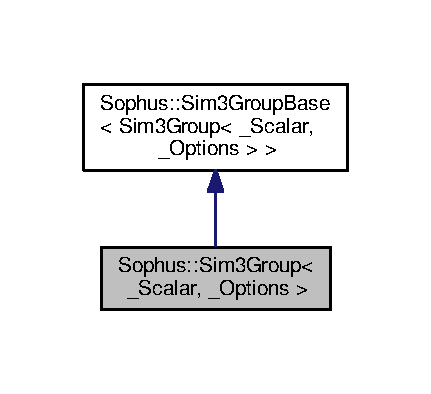
\includegraphics[width=207pt]{class_sophus_1_1_sim3_group__inherit__graph}
\end{center}
\end{figure}


Collaboration diagram for Sophus\+:\+:Sim3\+Group$<$ \+\_\+\+Scalar, \+\_\+\+Options $>$\+:
\nopagebreak
\begin{figure}[H]
\begin{center}
\leavevmode
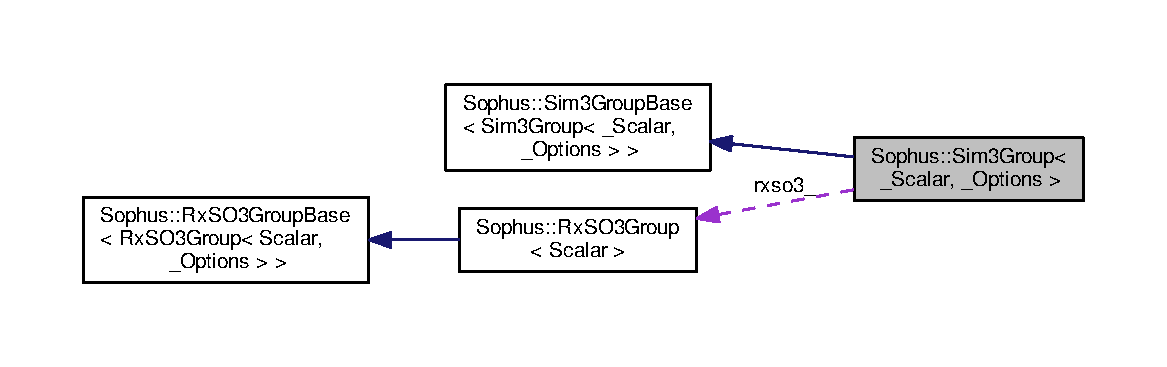
\includegraphics[width=350pt]{class_sophus_1_1_sim3_group__coll__graph}
\end{center}
\end{figure}
\subsection*{Public Types}
\begin{DoxyCompactItemize}
\item 
typedef internal\+::traits$<$ \hyperlink{class_sophus_1_1_sim3_group}{Sim3\+Group}$<$ \+\_\+\+Scalar, \+\_\+\+Options $>$ $>$\+::\hyperlink{class_sophus_1_1_sim3_group_a5db0ba2bb3fe2471006c9f366077c5bb}{Scalar} \hyperlink{class_sophus_1_1_sim3_group_a5db0ba2bb3fe2471006c9f366077c5bb}{Scalar}\hypertarget{class_sophus_1_1_sim3_group_a5db0ba2bb3fe2471006c9f366077c5bb}{}\label{class_sophus_1_1_sim3_group_a5db0ba2bb3fe2471006c9f366077c5bb}

\begin{DoxyCompactList}\small\item\em scalar type \end{DoxyCompactList}\item 
typedef internal\+::traits$<$ \hyperlink{class_sophus_1_1_sim3_group}{Sim3\+Group}$<$ \+\_\+\+Scalar, \+\_\+\+Options $>$ $>$\+::Rx\+S\+O3\+Type \& \hyperlink{class_sophus_1_1_sim3_group_a0010f4f99876a2165913382fa69117d8}{Rx\+S\+O3\+Reference}\hypertarget{class_sophus_1_1_sim3_group_a0010f4f99876a2165913382fa69117d8}{}\label{class_sophus_1_1_sim3_group_a0010f4f99876a2165913382fa69117d8}

\begin{DoxyCompactList}\small\item\em Rx\+S\+O3 reference type. \end{DoxyCompactList}\item 
typedef const internal\+::traits$<$ \hyperlink{class_sophus_1_1_sim3_group}{Sim3\+Group}$<$ \+\_\+\+Scalar, \+\_\+\+Options $>$ $>$\+::Rx\+S\+O3\+Type \& \hyperlink{class_sophus_1_1_sim3_group_a47e81f13e85164a1372395d978ab86fe}{Const\+Rx\+S\+O3\+Reference}\hypertarget{class_sophus_1_1_sim3_group_a47e81f13e85164a1372395d978ab86fe}{}\label{class_sophus_1_1_sim3_group_a47e81f13e85164a1372395d978ab86fe}

\begin{DoxyCompactList}\small\item\em Rx\+S\+O3 const reference type. \end{DoxyCompactList}\item 
typedef internal\+::traits$<$ \hyperlink{class_sophus_1_1_sim3_group}{Sim3\+Group}$<$ \+\_\+\+Scalar, \+\_\+\+Options $>$ $>$\+::Translation\+Type \& \hyperlink{class_sophus_1_1_sim3_group_a56c24566b7aed53015817b59e86989ce}{Translation\+Reference}\hypertarget{class_sophus_1_1_sim3_group_a56c24566b7aed53015817b59e86989ce}{}\label{class_sophus_1_1_sim3_group_a56c24566b7aed53015817b59e86989ce}

\begin{DoxyCompactList}\small\item\em translation reference type \end{DoxyCompactList}\item 
typedef const internal\+::traits$<$ \hyperlink{class_sophus_1_1_sim3_group}{Sim3\+Group}$<$ \+\_\+\+Scalar, \+\_\+\+Options $>$ $>$\+::Translation\+Type \& \hyperlink{class_sophus_1_1_sim3_group_a11a3c75cf3bdad1f730722cf1767e012}{Const\+Translation\+Reference}\hypertarget{class_sophus_1_1_sim3_group_a11a3c75cf3bdad1f730722cf1767e012}{}\label{class_sophus_1_1_sim3_group_a11a3c75cf3bdad1f730722cf1767e012}

\begin{DoxyCompactList}\small\item\em translation const reference type \end{DoxyCompactList}\item 
typedef \hyperlink{class_sophus_1_1_sim3_group_base_a93c8c564e3386709dc4cb2fc6d451dd8}{Base\+::\+Transformation} \hyperlink{class_sophus_1_1_sim3_group_a0b3a5b31501e1358aa760c91e128db9f}{Transformation}\hypertarget{class_sophus_1_1_sim3_group_a0b3a5b31501e1358aa760c91e128db9f}{}\label{class_sophus_1_1_sim3_group_a0b3a5b31501e1358aa760c91e128db9f}

\begin{DoxyCompactList}\small\item\em group transfomation type \end{DoxyCompactList}\item 
typedef \hyperlink{class_sophus_1_1_sim3_group_base_a4b50c6b94e402746e50076305781dc9d}{Base\+::\+Point} \hyperlink{class_sophus_1_1_sim3_group_a1848018ed54875cbfe8fc437cb02237d}{Point}\hypertarget{class_sophus_1_1_sim3_group_a1848018ed54875cbfe8fc437cb02237d}{}\label{class_sophus_1_1_sim3_group_a1848018ed54875cbfe8fc437cb02237d}

\begin{DoxyCompactList}\small\item\em point type \end{DoxyCompactList}\item 
typedef \hyperlink{class_sophus_1_1_sim3_group_base_a0f61582b6d8fa46ecbb40d70c87b632c}{Base\+::\+Tangent} \hyperlink{class_sophus_1_1_sim3_group_a4988923bd1230999bb6a9eef6439810b}{Tangent}\hypertarget{class_sophus_1_1_sim3_group_a4988923bd1230999bb6a9eef6439810b}{}\label{class_sophus_1_1_sim3_group_a4988923bd1230999bb6a9eef6439810b}

\begin{DoxyCompactList}\small\item\em tangent vector type \end{DoxyCompactList}\item 
typedef \hyperlink{class_sophus_1_1_sim3_group_base_a7aa93f325ac7b811db77652f488e8f03}{Base\+::\+Adjoint} \hyperlink{class_sophus_1_1_sim3_group_a0fd8d9f8b06a3996a404c5dc2208fe63}{Adjoint}\hypertarget{class_sophus_1_1_sim3_group_a0fd8d9f8b06a3996a404c5dc2208fe63}{}\label{class_sophus_1_1_sim3_group_a0fd8d9f8b06a3996a404c5dc2208fe63}

\begin{DoxyCompactList}\small\item\em adjoint transformation type \end{DoxyCompactList}\end{DoxyCompactItemize}
\subsection*{Public Member Functions}
\begin{DoxyCompactItemize}
\item 
E\+I\+G\+E\+N\+\_\+\+M\+A\+K\+E\+\_\+\+A\+L\+I\+G\+N\+E\+D\+\_\+\+O\+P\+E\+R\+A\+T\+O\+R\+\_\+\+N\+EW \hyperlink{class_sophus_1_1_sim3_group_a61cd6b6dd6a6700f56f3c1ed976ccf5a}{Sim3\+Group} ()
\begin{DoxyCompactList}\small\item\em Default constructor. \end{DoxyCompactList}\item 
{\footnotesize template$<$typename Other\+Derived $>$ }\\\hyperlink{class_sophus_1_1_sim3_group_a6cc33ac145da6d0597ceebb4f96b79c8}{Sim3\+Group} (const \hyperlink{class_sophus_1_1_sim3_group_base}{Sim3\+Group\+Base}$<$ Other\+Derived $>$ \&other)\hypertarget{class_sophus_1_1_sim3_group_a6cc33ac145da6d0597ceebb4f96b79c8}{}\label{class_sophus_1_1_sim3_group_a6cc33ac145da6d0597ceebb4f96b79c8}

\begin{DoxyCompactList}\small\item\em Copy constructor. \end{DoxyCompactList}\item 
{\footnotesize template$<$typename Other\+Derived $>$ }\\\hyperlink{class_sophus_1_1_sim3_group_aa6ffffa0d01b174133e8ab5dd53d4e96}{Sim3\+Group} (const \hyperlink{class_sophus_1_1_rx_s_o3_group_base}{Rx\+S\+O3\+Group\+Base}$<$ Other\+Derived $>$ \&\hyperlink{class_sophus_1_1_sim3_group_a4f8602d647961667444f0cb19fb553b1}{rxso3}, const \hyperlink{class_sophus_1_1_sim3_group_a1848018ed54875cbfe8fc437cb02237d}{Point} \&\hyperlink{class_sophus_1_1_sim3_group_ace8b98b369832930e647675b8c005d64}{translation})\hypertarget{class_sophus_1_1_sim3_group_aa6ffffa0d01b174133e8ab5dd53d4e96}{}\label{class_sophus_1_1_sim3_group_aa6ffffa0d01b174133e8ab5dd53d4e96}

\begin{DoxyCompactList}\small\item\em Constructor from Rx\+S\+O3 and translation vector. \end{DoxyCompactList}\item 
\hyperlink{class_sophus_1_1_sim3_group_a24b507674b877686c6dbd40a959abb09}{Sim3\+Group} (const Quaternion$<$ \hyperlink{class_sophus_1_1_sim3_group_a5db0ba2bb3fe2471006c9f366077c5bb}{Scalar} $>$ \&\hyperlink{class_sophus_1_1_sim3_group_base_a3629f9f036df49823d478e3692d23e82}{quaternion}, const \hyperlink{class_sophus_1_1_sim3_group_a1848018ed54875cbfe8fc437cb02237d}{Point} \&\hyperlink{class_sophus_1_1_sim3_group_ace8b98b369832930e647675b8c005d64}{translation})
\begin{DoxyCompactList}\small\item\em Constructor from quaternion and translation vector. \end{DoxyCompactList}\item 
\hyperlink{class_sophus_1_1_sim3_group_a178767e5571ad9e2f602e1c00fb28b61}{Sim3\+Group} (const Eigen\+::\+Matrix$<$ \hyperlink{class_sophus_1_1_sim3_group_a5db0ba2bb3fe2471006c9f366077c5bb}{Scalar}, 4, 4 $>$ \&T)
\begin{DoxyCompactList}\small\item\em Constructor from 4x4 matrix. \end{DoxyCompactList}\item 
E\+I\+G\+E\+N\+\_\+\+S\+T\+R\+O\+N\+G\+\_\+\+I\+N\+L\+I\+NE \hyperlink{class_sophus_1_1_sim3_group_a5db0ba2bb3fe2471006c9f366077c5bb}{Scalar} $\ast$ \hyperlink{class_sophus_1_1_sim3_group_ac422c2e56354fbf07e12e333345c6bd0}{data} ()
\item 
E\+I\+G\+E\+N\+\_\+\+S\+T\+R\+O\+N\+G\+\_\+\+I\+N\+L\+I\+NE const \hyperlink{class_sophus_1_1_sim3_group_a5db0ba2bb3fe2471006c9f366077c5bb}{Scalar} $\ast$ \hyperlink{class_sophus_1_1_sim3_group_a7b7c2858ddacde4c2a53d97d70d98ee3}{data} () const 
\item 
E\+I\+G\+E\+N\+\_\+\+S\+T\+R\+O\+N\+G\+\_\+\+I\+N\+L\+I\+NE \hyperlink{class_sophus_1_1_sim3_group_a0010f4f99876a2165913382fa69117d8}{Rx\+S\+O3\+Reference} \hyperlink{class_sophus_1_1_sim3_group_a4f8602d647961667444f0cb19fb553b1}{rxso3} ()\hypertarget{class_sophus_1_1_sim3_group_a4f8602d647961667444f0cb19fb553b1}{}\label{class_sophus_1_1_sim3_group_a4f8602d647961667444f0cb19fb553b1}

\begin{DoxyCompactList}\small\item\em Accessor of Rx\+S\+O3. \end{DoxyCompactList}\item 
E\+I\+G\+E\+N\+\_\+\+S\+T\+R\+O\+N\+G\+\_\+\+I\+N\+L\+I\+NE \hyperlink{class_sophus_1_1_sim3_group_a47e81f13e85164a1372395d978ab86fe}{Const\+Rx\+S\+O3\+Reference} \hyperlink{class_sophus_1_1_sim3_group_a54af37f660dccf8c687d7c714fb46234}{rxso3} () const \hypertarget{class_sophus_1_1_sim3_group_a54af37f660dccf8c687d7c714fb46234}{}\label{class_sophus_1_1_sim3_group_a54af37f660dccf8c687d7c714fb46234}

\begin{DoxyCompactList}\small\item\em Mutator of Rx\+S\+O3. \end{DoxyCompactList}\item 
E\+I\+G\+E\+N\+\_\+\+S\+T\+R\+O\+N\+G\+\_\+\+I\+N\+L\+I\+NE \hyperlink{class_sophus_1_1_sim3_group_a56c24566b7aed53015817b59e86989ce}{Translation\+Reference} \hyperlink{class_sophus_1_1_sim3_group_ace8b98b369832930e647675b8c005d64}{translation} ()\hypertarget{class_sophus_1_1_sim3_group_ace8b98b369832930e647675b8c005d64}{}\label{class_sophus_1_1_sim3_group_ace8b98b369832930e647675b8c005d64}

\begin{DoxyCompactList}\small\item\em Mutator of translation vector. \end{DoxyCompactList}\item 
E\+I\+G\+E\+N\+\_\+\+S\+T\+R\+O\+N\+G\+\_\+\+I\+N\+L\+I\+NE \hyperlink{class_sophus_1_1_sim3_group_a11a3c75cf3bdad1f730722cf1767e012}{Const\+Translation\+Reference} \hyperlink{class_sophus_1_1_sim3_group_a7e82e871f647e2620020782e3b1ca503}{translation} () const \hypertarget{class_sophus_1_1_sim3_group_a7e82e871f647e2620020782e3b1ca503}{}\label{class_sophus_1_1_sim3_group_a7e82e871f647e2620020782e3b1ca503}

\begin{DoxyCompactList}\small\item\em Accessor of translation vector. \end{DoxyCompactList}\end{DoxyCompactItemize}
\subsection*{Static Public Attributes}
\begin{DoxyCompactItemize}
\item 
static const int \hyperlink{class_sophus_1_1_sim3_group_ac073510c872e1fbbf0e0cf1ec0828f58}{DoF} = Base\+::\+DoF\hypertarget{class_sophus_1_1_sim3_group_ac073510c872e1fbbf0e0cf1ec0828f58}{}\label{class_sophus_1_1_sim3_group_ac073510c872e1fbbf0e0cf1ec0828f58}

\begin{DoxyCompactList}\small\item\em degree of freedom of group \end{DoxyCompactList}\item 
static const int \hyperlink{class_sophus_1_1_sim3_group_a00e6e0e97d7f40825215292fea37e9c4}{num\+\_\+parameters} = Base\+::num\+\_\+parameters\hypertarget{class_sophus_1_1_sim3_group_a00e6e0e97d7f40825215292fea37e9c4}{}\label{class_sophus_1_1_sim3_group_a00e6e0e97d7f40825215292fea37e9c4}

\begin{DoxyCompactList}\small\item\em number of internal parameters used \end{DoxyCompactList}\item 
static const int \hyperlink{class_sophus_1_1_sim3_group_ac7127f3be157379ee4c3e89030964791}{N} = Base\+::N\hypertarget{class_sophus_1_1_sim3_group_ac7127f3be157379ee4c3e89030964791}{}\label{class_sophus_1_1_sim3_group_ac7127f3be157379ee4c3e89030964791}

\begin{DoxyCompactList}\small\item\em group transformations are NxN matrices \end{DoxyCompactList}\end{DoxyCompactItemize}
\subsection*{Protected Attributes}
\begin{DoxyCompactItemize}
\item 
\hyperlink{class_sophus_1_1_rx_s_o3_group}{Sophus\+::\+Rx\+S\+O3\+Group}$<$ \hyperlink{class_sophus_1_1_sim3_group_a5db0ba2bb3fe2471006c9f366077c5bb}{Scalar} $>$ {\bfseries rxso3\+\_\+}\hypertarget{class_sophus_1_1_sim3_group_a5f13e46bdd9b164eb2922bab66f826ad}{}\label{class_sophus_1_1_sim3_group_a5f13e46bdd9b164eb2922bab66f826ad}

\item 
Matrix$<$ \hyperlink{class_sophus_1_1_sim3_group_a5db0ba2bb3fe2471006c9f366077c5bb}{Scalar}, 3, 1 $>$ {\bfseries translation\+\_\+}\hypertarget{class_sophus_1_1_sim3_group_a93fd08a5b0a4a2c3ecec7990c0c7c51c}{}\label{class_sophus_1_1_sim3_group_a93fd08a5b0a4a2c3ecec7990c0c7c51c}

\end{DoxyCompactItemize}
\subsection*{Additional Inherited Members}


\subsection{Detailed Description}
\subsubsection*{template$<$typename \+\_\+\+Scalar, int \+\_\+\+Options$>$\\*
class Sophus\+::\+Sim3\+Group$<$ \+\_\+\+Scalar, \+\_\+\+Options $>$}

Sim3 default type -\/ Constructors and default storage for Sim3 Type. 

Definition at line 33 of file sim3.\+hpp.



\subsection{Constructor \& Destructor Documentation}
\index{Sophus\+::\+Sim3\+Group@{Sophus\+::\+Sim3\+Group}!Sim3\+Group@{Sim3\+Group}}
\index{Sim3\+Group@{Sim3\+Group}!Sophus\+::\+Sim3\+Group@{Sophus\+::\+Sim3\+Group}}
\subsubsection[{\texorpdfstring{Sim3\+Group()}{Sim3Group()}}]{\setlength{\rightskip}{0pt plus 5cm}template$<$typename \+\_\+\+Scalar, int \+\_\+\+Options$>$ E\+I\+G\+E\+N\+\_\+\+M\+A\+K\+E\+\_\+\+A\+L\+I\+G\+N\+E\+D\+\_\+\+O\+P\+E\+R\+A\+T\+O\+R\+\_\+\+N\+EW {\bf Sophus\+::\+Sim3\+Group}$<$ \+\_\+\+Scalar, \+\_\+\+Options $>$\+::{\bf Sim3\+Group} (
\begin{DoxyParamCaption}
{}
\end{DoxyParamCaption}
)\hspace{0.3cm}{\ttfamily [inline]}}\hypertarget{class_sophus_1_1_sim3_group_a61cd6b6dd6a6700f56f3c1ed976ccf5a}{}\label{class_sophus_1_1_sim3_group_a61cd6b6dd6a6700f56f3c1ed976ccf5a}


Default constructor. 

Initialize Quaternion to identity rotation and translation to zero. 

Definition at line 696 of file sim3.\+hpp.

\index{Sophus\+::\+Sim3\+Group@{Sophus\+::\+Sim3\+Group}!Sim3\+Group@{Sim3\+Group}}
\index{Sim3\+Group@{Sim3\+Group}!Sophus\+::\+Sim3\+Group@{Sophus\+::\+Sim3\+Group}}
\subsubsection[{\texorpdfstring{Sim3\+Group(const Quaternion$<$ Scalar $>$ \&quaternion, const Point \&translation)}{Sim3Group(const Quaternion< Scalar > &quaternion, const Point &translation)}}]{\setlength{\rightskip}{0pt plus 5cm}template$<$typename \+\_\+\+Scalar, int \+\_\+\+Options$>$ {\bf Sophus\+::\+Sim3\+Group}$<$ \+\_\+\+Scalar, \+\_\+\+Options $>$\+::{\bf Sim3\+Group} (
\begin{DoxyParamCaption}
\item[{const Quaternion$<$ {\bf Scalar} $>$ \&}]{quaternion, }
\item[{const {\bf Point} \&}]{translation}
\end{DoxyParamCaption}
)\hspace{0.3cm}{\ttfamily [inline]}}\hypertarget{class_sophus_1_1_sim3_group_a24b507674b877686c6dbd40a959abb09}{}\label{class_sophus_1_1_sim3_group_a24b507674b877686c6dbd40a959abb09}


Constructor from quaternion and translation vector. 

\begin{DoxyPrecond}{Precondition}
quaternion must not be zero 
\end{DoxyPrecond}


Definition at line 724 of file sim3.\+hpp.

\index{Sophus\+::\+Sim3\+Group@{Sophus\+::\+Sim3\+Group}!Sim3\+Group@{Sim3\+Group}}
\index{Sim3\+Group@{Sim3\+Group}!Sophus\+::\+Sim3\+Group@{Sophus\+::\+Sim3\+Group}}
\subsubsection[{\texorpdfstring{Sim3\+Group(const Eigen\+::\+Matrix$<$ Scalar, 4, 4 $>$ \&\+T)}{Sim3Group(const Eigen::Matrix< Scalar, 4, 4 > &T)}}]{\setlength{\rightskip}{0pt plus 5cm}template$<$typename \+\_\+\+Scalar, int \+\_\+\+Options$>$ {\bf Sophus\+::\+Sim3\+Group}$<$ \+\_\+\+Scalar, \+\_\+\+Options $>$\+::{\bf Sim3\+Group} (
\begin{DoxyParamCaption}
\item[{const Eigen\+::\+Matrix$<$ {\bf Scalar}, 4, 4 $>$ \&}]{T}
\end{DoxyParamCaption}
)\hspace{0.3cm}{\ttfamily [inline]}, {\ttfamily [explicit]}}\hypertarget{class_sophus_1_1_sim3_group_a178767e5571ad9e2f602e1c00fb28b61}{}\label{class_sophus_1_1_sim3_group_a178767e5571ad9e2f602e1c00fb28b61}


Constructor from 4x4 matrix. 

\begin{DoxyPrecond}{Precondition}
top-\/left 3x3 sub-\/matrix need to be \char`\"{}scaled orthogonal\char`\"{} with positive determinant of 
\end{DoxyPrecond}


Definition at line 736 of file sim3.\+hpp.



\subsection{Member Function Documentation}
\index{Sophus\+::\+Sim3\+Group@{Sophus\+::\+Sim3\+Group}!data@{data}}
\index{data@{data}!Sophus\+::\+Sim3\+Group@{Sophus\+::\+Sim3\+Group}}
\subsubsection[{\texorpdfstring{data()}{data()}}]{\setlength{\rightskip}{0pt plus 5cm}template$<$typename \+\_\+\+Scalar, int \+\_\+\+Options$>$ E\+I\+G\+E\+N\+\_\+\+S\+T\+R\+O\+N\+G\+\_\+\+I\+N\+L\+I\+NE {\bf Scalar}$\ast$ {\bf Sophus\+::\+Sim3\+Group}$<$ \+\_\+\+Scalar, \+\_\+\+Options $>$\+::data (
\begin{DoxyParamCaption}
{}
\end{DoxyParamCaption}
)\hspace{0.3cm}{\ttfamily [inline]}}\hypertarget{class_sophus_1_1_sim3_group_ac422c2e56354fbf07e12e333345c6bd0}{}\label{class_sophus_1_1_sim3_group_ac422c2e56354fbf07e12e333345c6bd0}
\begin{DoxyReturn}{Returns}
pointer to internal data
\end{DoxyReturn}
This provides unsafe read/write access to internal data. Sim3 is represented by a pair of an Rx\+S\+O3 element (4 parameters) and translation vector (three parameters).

Note\+: The first three Scalars represent the imaginary parts, while the 

Definition at line 751 of file sim3.\+hpp.

\index{Sophus\+::\+Sim3\+Group@{Sophus\+::\+Sim3\+Group}!data@{data}}
\index{data@{data}!Sophus\+::\+Sim3\+Group@{Sophus\+::\+Sim3\+Group}}
\subsubsection[{\texorpdfstring{data() const }{data() const }}]{\setlength{\rightskip}{0pt plus 5cm}template$<$typename \+\_\+\+Scalar, int \+\_\+\+Options$>$ E\+I\+G\+E\+N\+\_\+\+S\+T\+R\+O\+N\+G\+\_\+\+I\+N\+L\+I\+NE const {\bf Scalar}$\ast$ {\bf Sophus\+::\+Sim3\+Group}$<$ \+\_\+\+Scalar, \+\_\+\+Options $>$\+::data (
\begin{DoxyParamCaption}
{}
\end{DoxyParamCaption}
) const\hspace{0.3cm}{\ttfamily [inline]}}\hypertarget{class_sophus_1_1_sim3_group_a7b7c2858ddacde4c2a53d97d70d98ee3}{}\label{class_sophus_1_1_sim3_group_a7b7c2858ddacde4c2a53d97d70d98ee3}
\begin{DoxyReturn}{Returns}
const pointer to internal data
\end{DoxyReturn}
Const version of \hyperlink{class_sophus_1_1_sim3_group_ac422c2e56354fbf07e12e333345c6bd0}{data()}. 

Definition at line 762 of file sim3.\+hpp.



The documentation for this class was generated from the following file\+:\begin{DoxyCompactItemize}
\item 
include/\+Sophus/sophus/sim3.\+hpp\end{DoxyCompactItemize}

\hypertarget{class_sophus_1_1_sim3_group_base}{}\section{Sophus\+:\+:Sim3\+Group\+Base$<$ Derived $>$ Class Template Reference}
\label{class_sophus_1_1_sim3_group_base}\index{Sophus\+::\+Sim3\+Group\+Base$<$ Derived $>$@{Sophus\+::\+Sim3\+Group\+Base$<$ Derived $>$}}


Sim3 base type -\/ implements Sim3 class but is storage agnostic.  




{\ttfamily \#include $<$sim3.\+hpp$>$}

\subsection*{Public Types}
\begin{DoxyCompactItemize}
\item 
typedef internal\+::traits$<$ Derived $>$\+::\hyperlink{class_sophus_1_1_sim3_group_base_abcf3d57b9fcc425bbc367a85a45a8092}{Scalar} \hyperlink{class_sophus_1_1_sim3_group_base_abcf3d57b9fcc425bbc367a85a45a8092}{Scalar}\hypertarget{class_sophus_1_1_sim3_group_base_abcf3d57b9fcc425bbc367a85a45a8092}{}\label{class_sophus_1_1_sim3_group_base_abcf3d57b9fcc425bbc367a85a45a8092}

\begin{DoxyCompactList}\small\item\em scalar type \end{DoxyCompactList}\item 
typedef internal\+::traits$<$ Derived $>$\+::Translation\+Type \& \hyperlink{class_sophus_1_1_sim3_group_base_a0491010ffcd9971dea880f7bce6910e5}{Translation\+Reference}\hypertarget{class_sophus_1_1_sim3_group_base_a0491010ffcd9971dea880f7bce6910e5}{}\label{class_sophus_1_1_sim3_group_base_a0491010ffcd9971dea880f7bce6910e5}

\begin{DoxyCompactList}\small\item\em translation reference type \end{DoxyCompactList}\item 
typedef const internal\+::traits$<$ Derived $>$\+::Translation\+Type \& \hyperlink{class_sophus_1_1_sim3_group_base_aee08d851899efe59011fb1b58dbf1139}{Const\+Translation\+Reference}\hypertarget{class_sophus_1_1_sim3_group_base_aee08d851899efe59011fb1b58dbf1139}{}\label{class_sophus_1_1_sim3_group_base_aee08d851899efe59011fb1b58dbf1139}

\begin{DoxyCompactList}\small\item\em translation const reference type \end{DoxyCompactList}\item 
typedef internal\+::traits$<$ Derived $>$\+::Rx\+S\+O3\+Type \& \hyperlink{class_sophus_1_1_sim3_group_base_a12827cf23c0ef3b94adbb088e8be891e}{Rx\+S\+O3\+Reference}\hypertarget{class_sophus_1_1_sim3_group_base_a12827cf23c0ef3b94adbb088e8be891e}{}\label{class_sophus_1_1_sim3_group_base_a12827cf23c0ef3b94adbb088e8be891e}

\begin{DoxyCompactList}\small\item\em Rx\+S\+O3 reference type. \end{DoxyCompactList}\item 
typedef const internal\+::traits$<$ Derived $>$\+::Rx\+S\+O3\+Type \& \hyperlink{class_sophus_1_1_sim3_group_base_ae170af2cf9301830de6fac478b322498}{Const\+Rx\+S\+O3\+Reference}\hypertarget{class_sophus_1_1_sim3_group_base_ae170af2cf9301830de6fac478b322498}{}\label{class_sophus_1_1_sim3_group_base_ae170af2cf9301830de6fac478b322498}

\begin{DoxyCompactList}\small\item\em Rx\+S\+O3 const reference type. \end{DoxyCompactList}\item 
typedef Matrix$<$ \hyperlink{class_sophus_1_1_sim3_group_base_abcf3d57b9fcc425bbc367a85a45a8092}{Scalar}, \hyperlink{class_sophus_1_1_sim3_group_base_a255dcef6539b58cd1b78ab90fa5899fb}{N}, \hyperlink{class_sophus_1_1_sim3_group_base_a255dcef6539b58cd1b78ab90fa5899fb}{N} $>$ \hyperlink{class_sophus_1_1_sim3_group_base_a93c8c564e3386709dc4cb2fc6d451dd8}{Transformation}\hypertarget{class_sophus_1_1_sim3_group_base_a93c8c564e3386709dc4cb2fc6d451dd8}{}\label{class_sophus_1_1_sim3_group_base_a93c8c564e3386709dc4cb2fc6d451dd8}

\begin{DoxyCompactList}\small\item\em group transfomation type \end{DoxyCompactList}\item 
typedef Matrix$<$ \hyperlink{class_sophus_1_1_sim3_group_base_abcf3d57b9fcc425bbc367a85a45a8092}{Scalar}, 3, 1 $>$ \hyperlink{class_sophus_1_1_sim3_group_base_a4b50c6b94e402746e50076305781dc9d}{Point}\hypertarget{class_sophus_1_1_sim3_group_base_a4b50c6b94e402746e50076305781dc9d}{}\label{class_sophus_1_1_sim3_group_base_a4b50c6b94e402746e50076305781dc9d}

\begin{DoxyCompactList}\small\item\em point type \end{DoxyCompactList}\item 
typedef Matrix$<$ \hyperlink{class_sophus_1_1_sim3_group_base_abcf3d57b9fcc425bbc367a85a45a8092}{Scalar}, \hyperlink{class_sophus_1_1_sim3_group_base_a15603751ad5a1018653b7e33480c7325}{DoF}, 1 $>$ \hyperlink{class_sophus_1_1_sim3_group_base_a0f61582b6d8fa46ecbb40d70c87b632c}{Tangent}\hypertarget{class_sophus_1_1_sim3_group_base_a0f61582b6d8fa46ecbb40d70c87b632c}{}\label{class_sophus_1_1_sim3_group_base_a0f61582b6d8fa46ecbb40d70c87b632c}

\begin{DoxyCompactList}\small\item\em tangent vector type \end{DoxyCompactList}\item 
typedef Matrix$<$ \hyperlink{class_sophus_1_1_sim3_group_base_abcf3d57b9fcc425bbc367a85a45a8092}{Scalar}, \hyperlink{class_sophus_1_1_sim3_group_base_a15603751ad5a1018653b7e33480c7325}{DoF}, \hyperlink{class_sophus_1_1_sim3_group_base_a15603751ad5a1018653b7e33480c7325}{DoF} $>$ \hyperlink{class_sophus_1_1_sim3_group_base_a7aa93f325ac7b811db77652f488e8f03}{Adjoint}\hypertarget{class_sophus_1_1_sim3_group_base_a7aa93f325ac7b811db77652f488e8f03}{}\label{class_sophus_1_1_sim3_group_base_a7aa93f325ac7b811db77652f488e8f03}

\begin{DoxyCompactList}\small\item\em adjoint transformation type \end{DoxyCompactList}\end{DoxyCompactItemize}
\subsection*{Public Member Functions}
\begin{DoxyCompactItemize}
\item 
const \hyperlink{class_sophus_1_1_sim3_group_base_a7aa93f325ac7b811db77652f488e8f03}{Adjoint} \hyperlink{class_sophus_1_1_sim3_group_base_ab68ea48a89f018d3d298001a51cd6b95}{Adj} () const 
\begin{DoxyCompactList}\small\item\em Adjoint transformation. \end{DoxyCompactList}\item 
{\footnotesize template$<$typename New\+Scalar\+Type $>$ }\\\hyperlink{class_sophus_1_1_sim3_group}{Sim3\+Group}$<$ New\+Scalar\+Type $>$ \hyperlink{class_sophus_1_1_sim3_group_base_afb710f8ef8ee6f6168dea80fe119d131}{cast} () const 
\item 
void \hyperlink{class_sophus_1_1_sim3_group_base_a83dfde5b319dc9055f5723d29a45ed89}{fast\+Multiply} (const \hyperlink{class_sophus_1_1_sim3_group}{Sim3\+Group}$<$ \hyperlink{class_sophus_1_1_sim3_group_base_abcf3d57b9fcc425bbc367a85a45a8092}{Scalar} $>$ \&other)
\begin{DoxyCompactList}\small\item\em In-\/place group multiplication. \end{DoxyCompactList}\item 
const \hyperlink{class_sophus_1_1_sim3_group}{Sim3\+Group}$<$ \hyperlink{class_sophus_1_1_sim3_group_base_abcf3d57b9fcc425bbc367a85a45a8092}{Scalar} $>$ \hyperlink{class_sophus_1_1_sim3_group_base_a21debb906ffbeda23394fbddea8f3acd}{inverse} () const 
\item 
const \hyperlink{class_sophus_1_1_sim3_group_base_a0f61582b6d8fa46ecbb40d70c87b632c}{Tangent} \hyperlink{class_sophus_1_1_sim3_group_base_ae8417db9c9a27c4a99955561062d48fc}{log} () const 
\begin{DoxyCompactList}\small\item\em Logarithmic map. \end{DoxyCompactList}\item 
const \hyperlink{class_sophus_1_1_sim3_group_base_a93c8c564e3386709dc4cb2fc6d451dd8}{Transformation} \hyperlink{class_sophus_1_1_sim3_group_base_a4cce2bd5ded85614bedd1e13b7efe494}{matrix} () const 
\item 
const Matrix$<$ \hyperlink{class_sophus_1_1_sim3_group_base_abcf3d57b9fcc425bbc367a85a45a8092}{Scalar}, 3, 4 $>$ \hyperlink{class_sophus_1_1_sim3_group_base_a7894ea86d497e4dee880e669817e3146}{matrix3x4} () const 
\item 
{\footnotesize template$<$typename Other\+Derived $>$ }\\\hyperlink{class_sophus_1_1_sim3_group_base}{Sim3\+Group\+Base}$<$ Derived $>$ \& \hyperlink{class_sophus_1_1_sim3_group_base_a05c83b534686d7e048307ca962c3d3b3}{operator=} (const \hyperlink{class_sophus_1_1_sim3_group_base}{Sim3\+Group\+Base}$<$ Other\+Derived $>$ \&other)\hypertarget{class_sophus_1_1_sim3_group_base_a05c83b534686d7e048307ca962c3d3b3}{}\label{class_sophus_1_1_sim3_group_base_a05c83b534686d7e048307ca962c3d3b3}

\begin{DoxyCompactList}\small\item\em Assignment operator. \end{DoxyCompactList}\item 
const \hyperlink{class_sophus_1_1_sim3_group}{Sim3\+Group}$<$ \hyperlink{class_sophus_1_1_sim3_group_base_abcf3d57b9fcc425bbc367a85a45a8092}{Scalar} $>$ \hyperlink{class_sophus_1_1_sim3_group_base_a2870e3d6011b9a8a9b89b9ad21a2c00f}{operator$\ast$} (const \hyperlink{class_sophus_1_1_sim3_group}{Sim3\+Group}$<$ \hyperlink{class_sophus_1_1_sim3_group_base_abcf3d57b9fcc425bbc367a85a45a8092}{Scalar} $>$ \&other) const 
\begin{DoxyCompactList}\small\item\em Group multiplication. \end{DoxyCompactList}\item 
const \hyperlink{class_sophus_1_1_sim3_group_base_a4b50c6b94e402746e50076305781dc9d}{Point} \hyperlink{class_sophus_1_1_sim3_group_base_a39e689b5b3709c2fbfeda9a4485fc173}{operator$\ast$} (const \hyperlink{class_sophus_1_1_sim3_group_base_a4b50c6b94e402746e50076305781dc9d}{Point} \&p) const 
\begin{DoxyCompactList}\small\item\em Group action on $ \mathbf{R}^3 $. \end{DoxyCompactList}\item 
void \hyperlink{class_sophus_1_1_sim3_group_base_abd2cea80fd7e2216e1ca9f1fa8681b67}{operator$\ast$=} (const \hyperlink{class_sophus_1_1_sim3_group}{Sim3\+Group}$<$ \hyperlink{class_sophus_1_1_sim3_group_base_abcf3d57b9fcc425bbc367a85a45a8092}{Scalar} $>$ \&other)
\begin{DoxyCompactList}\small\item\em In-\/place group multiplication. \end{DoxyCompactList}\item 
internal\+::traits$<$ Derived $>$\+::Rx\+S\+O3\+Type\+::\+Quaternion\+Reference \hyperlink{class_sophus_1_1_sim3_group_base_a3629f9f036df49823d478e3692d23e82}{quaternion} ()\hypertarget{class_sophus_1_1_sim3_group_base_a3629f9f036df49823d478e3692d23e82}{}\label{class_sophus_1_1_sim3_group_base_a3629f9f036df49823d478e3692d23e82}

\begin{DoxyCompactList}\small\item\em Mutator of quaternion. \end{DoxyCompactList}\item 
internal\+::traits$<$ Derived $>$\+::Rx\+S\+O3\+Type\+::\+Const\+Quaternion\+Reference \hyperlink{class_sophus_1_1_sim3_group_base_a1c9089b2ac5d29261b1665f8e5c19876}{quaternion} () const \hypertarget{class_sophus_1_1_sim3_group_base_a1c9089b2ac5d29261b1665f8e5c19876}{}\label{class_sophus_1_1_sim3_group_base_a1c9089b2ac5d29261b1665f8e5c19876}

\begin{DoxyCompactList}\small\item\em Accessor of quaternion. \end{DoxyCompactList}\item 
\hyperlink{class_sophus_1_1_rx_s_o3_group}{E\+I\+G\+E\+N\+\_\+\+D\+E\+P\+R\+E\+C\+A\+T\+ED} const \hyperlink{class_sophus_1_1_sim3_group_base_a93c8c564e3386709dc4cb2fc6d451dd8}{Transformation} \hyperlink{class_sophus_1_1_sim3_group_base_a89e95392c0cd09d50c6035acd7101677}{rotation\+\_\+matrix} () const 
\item 
const Matrix$<$ \hyperlink{class_sophus_1_1_sim3_group_base_abcf3d57b9fcc425bbc367a85a45a8092}{Scalar}, 3, 3 $>$ \hyperlink{class_sophus_1_1_sim3_group_base_aa65d0a5e41074a979e574bf6aac62694}{rotation\+Matrix} () const 
\item 
E\+I\+G\+E\+N\+\_\+\+S\+T\+R\+O\+N\+G\+\_\+\+I\+N\+L\+I\+NE \hyperlink{class_sophus_1_1_sim3_group_base_a12827cf23c0ef3b94adbb088e8be891e}{Rx\+S\+O3\+Reference} \hyperlink{class_sophus_1_1_sim3_group_base_a352ae52574d5686aa113e008d95ebb64}{rxso3} ()\hypertarget{class_sophus_1_1_sim3_group_base_a352ae52574d5686aa113e008d95ebb64}{}\label{class_sophus_1_1_sim3_group_base_a352ae52574d5686aa113e008d95ebb64}

\begin{DoxyCompactList}\small\item\em Mutator of Rx\+S\+O3 group. \end{DoxyCompactList}\item 
E\+I\+G\+E\+N\+\_\+\+S\+T\+R\+O\+N\+G\+\_\+\+I\+N\+L\+I\+NE \hyperlink{class_sophus_1_1_sim3_group_base_ae170af2cf9301830de6fac478b322498}{Const\+Rx\+S\+O3\+Reference} \hyperlink{class_sophus_1_1_sim3_group_base_a45c09e43e821147ec1a33efda4d92b7b}{rxso3} () const \hypertarget{class_sophus_1_1_sim3_group_base_a45c09e43e821147ec1a33efda4d92b7b}{}\label{class_sophus_1_1_sim3_group_base_a45c09e43e821147ec1a33efda4d92b7b}

\begin{DoxyCompactList}\small\item\em Accessor of Rx\+S\+O3 group. \end{DoxyCompactList}\item 
E\+I\+G\+E\+N\+\_\+\+S\+T\+R\+O\+N\+G\+\_\+\+I\+N\+L\+I\+NE const \hyperlink{class_sophus_1_1_sim3_group_base_abcf3d57b9fcc425bbc367a85a45a8092}{Scalar} \hyperlink{class_sophus_1_1_sim3_group_base_a31cf579b7bc4d3b3358921f3501700cd}{scale} () const 
\item 
void \hyperlink{class_sophus_1_1_sim3_group_base_a5af76b731517484c70bff80ea9c3357f}{set\+Rotation\+Matrix} (const Matrix$<$ \hyperlink{class_sophus_1_1_sim3_group_base_abcf3d57b9fcc425bbc367a85a45a8092}{Scalar}, 3, 3 $>$ \&R)
\begin{DoxyCompactList}\small\item\em Setter of quaternion using rotation matrix, leaves scale untouched. \end{DoxyCompactList}\item 
E\+I\+G\+E\+N\+\_\+\+S\+T\+R\+O\+N\+G\+\_\+\+I\+N\+L\+I\+NE void \hyperlink{class_sophus_1_1_sim3_group_base_a04b97a30687ff11cd2c1192902b495e0}{set\+Scale} (const \hyperlink{class_sophus_1_1_sim3_group_base_abcf3d57b9fcc425bbc367a85a45a8092}{Scalar} \&\hyperlink{class_sophus_1_1_sim3_group_base_a31cf579b7bc4d3b3358921f3501700cd}{scale})\hypertarget{class_sophus_1_1_sim3_group_base_a04b97a30687ff11cd2c1192902b495e0}{}\label{class_sophus_1_1_sim3_group_base_a04b97a30687ff11cd2c1192902b495e0}

\begin{DoxyCompactList}\small\item\em Scale setter. \end{DoxyCompactList}\item 
void \hyperlink{class_sophus_1_1_sim3_group_base_ad5f6f6386cae4ad0af6c13825a4eca78}{set\+Scaled\+Rotation\+Matrix} (const Matrix$<$ \hyperlink{class_sophus_1_1_sim3_group_base_abcf3d57b9fcc425bbc367a85a45a8092}{Scalar}, 3, 3 $>$ \&sR)
\begin{DoxyCompactList}\small\item\em Setter of quaternion using scaled rotation matrix. \end{DoxyCompactList}\item 
E\+I\+G\+E\+N\+\_\+\+S\+T\+R\+O\+N\+G\+\_\+\+I\+N\+L\+I\+NE \hyperlink{class_sophus_1_1_sim3_group_base_a0491010ffcd9971dea880f7bce6910e5}{Translation\+Reference} \hyperlink{class_sophus_1_1_sim3_group_base_ae0a27d16e3c355fcf6977f1875f82ba6}{translation} ()\hypertarget{class_sophus_1_1_sim3_group_base_ae0a27d16e3c355fcf6977f1875f82ba6}{}\label{class_sophus_1_1_sim3_group_base_ae0a27d16e3c355fcf6977f1875f82ba6}

\begin{DoxyCompactList}\small\item\em Mutator of translation vector. \end{DoxyCompactList}\item 
E\+I\+G\+E\+N\+\_\+\+S\+T\+R\+O\+N\+G\+\_\+\+I\+N\+L\+I\+NE \hyperlink{class_sophus_1_1_sim3_group_base_aee08d851899efe59011fb1b58dbf1139}{Const\+Translation\+Reference} \hyperlink{class_sophus_1_1_sim3_group_base_a5a6f1907abc5a581e4fca69dbb09687c}{translation} () const \hypertarget{class_sophus_1_1_sim3_group_base_a5a6f1907abc5a581e4fca69dbb09687c}{}\label{class_sophus_1_1_sim3_group_base_a5a6f1907abc5a581e4fca69dbb09687c}

\begin{DoxyCompactList}\small\item\em Accessor of translation vector. \end{DoxyCompactList}\end{DoxyCompactItemize}
\subsection*{Static Public Member Functions}
\begin{DoxyCompactItemize}
\item 
static const \hyperlink{class_sophus_1_1_sim3_group_base_a7aa93f325ac7b811db77652f488e8f03}{Adjoint} \hyperlink{class_sophus_1_1_sim3_group_base_a75d815e06f09b40f27f19cb8d91e4b11}{d\+\_\+lie\+Bracketab\+\_\+by\+\_\+d\+\_\+a} (const \hyperlink{class_sophus_1_1_sim3_group_base_a0f61582b6d8fa46ecbb40d70c87b632c}{Tangent} \&b)
\item 
static const \hyperlink{class_sophus_1_1_sim3_group}{Sim3\+Group}$<$ \hyperlink{class_sophus_1_1_sim3_group_base_abcf3d57b9fcc425bbc367a85a45a8092}{Scalar} $>$ \hyperlink{class_sophus_1_1_sim3_group_base_ac39ec02a41087c306c333e7104def94c}{exp} (const \hyperlink{class_sophus_1_1_sim3_group_base_a0f61582b6d8fa46ecbb40d70c87b632c}{Tangent} \&a)
\begin{DoxyCompactList}\small\item\em Group exponential. \end{DoxyCompactList}\item 
static const \hyperlink{class_sophus_1_1_sim3_group_base_a93c8c564e3386709dc4cb2fc6d451dd8}{Transformation} \hyperlink{class_sophus_1_1_sim3_group_base_a69f3e5315c09c13a1776c8cdde52bd99}{generator} (int i)
\begin{DoxyCompactList}\small\item\em Generators. \end{DoxyCompactList}\item 
static const \hyperlink{class_sophus_1_1_sim3_group_base_a93c8c564e3386709dc4cb2fc6d451dd8}{Transformation} \hyperlink{class_sophus_1_1_sim3_group_base_a4260919b9987a953c96f1e363e36550b}{hat} (const \hyperlink{class_sophus_1_1_sim3_group_base_a0f61582b6d8fa46ecbb40d70c87b632c}{Tangent} \&v)
\begin{DoxyCompactList}\small\item\em hat-\/operator \end{DoxyCompactList}\item 
static const \hyperlink{class_sophus_1_1_sim3_group_base_a0f61582b6d8fa46ecbb40d70c87b632c}{Tangent} \hyperlink{class_sophus_1_1_sim3_group_base_a2d00f2fe3d14bef278f9e858bec68b0b}{lie\+Bracket} (const \hyperlink{class_sophus_1_1_sim3_group_base_a0f61582b6d8fa46ecbb40d70c87b632c}{Tangent} \&a, const \hyperlink{class_sophus_1_1_sim3_group_base_a0f61582b6d8fa46ecbb40d70c87b632c}{Tangent} \&b)
\begin{DoxyCompactList}\small\item\em Lie bracket. \end{DoxyCompactList}\item 
static const \hyperlink{class_sophus_1_1_sim3_group_base_a0f61582b6d8fa46ecbb40d70c87b632c}{Tangent} \hyperlink{class_sophus_1_1_sim3_group_base_abfa0c8c65937d72a5de61ca77984229a}{log} (const \hyperlink{class_sophus_1_1_sim3_group}{Sim3\+Group}$<$ \hyperlink{class_sophus_1_1_sim3_group_base_abcf3d57b9fcc425bbc367a85a45a8092}{Scalar} $>$ \&other)
\begin{DoxyCompactList}\small\item\em Logarithmic map. \end{DoxyCompactList}\item 
static const \hyperlink{class_sophus_1_1_sim3_group_base_a0f61582b6d8fa46ecbb40d70c87b632c}{Tangent} \hyperlink{class_sophus_1_1_sim3_group_base_abbe5ee89ea9ffb584c5ee93ed61e42a3}{vee} (const \hyperlink{class_sophus_1_1_sim3_group_base_a93c8c564e3386709dc4cb2fc6d451dd8}{Transformation} \&Omega)
\begin{DoxyCompactList}\small\item\em vee-\/operator \end{DoxyCompactList}\end{DoxyCompactItemize}
\subsection*{Static Public Attributes}
\begin{DoxyCompactItemize}
\item 
static const int \hyperlink{class_sophus_1_1_sim3_group_base_a15603751ad5a1018653b7e33480c7325}{DoF} = 7\hypertarget{class_sophus_1_1_sim3_group_base_a15603751ad5a1018653b7e33480c7325}{}\label{class_sophus_1_1_sim3_group_base_a15603751ad5a1018653b7e33480c7325}

\begin{DoxyCompactList}\small\item\em degree of freedom of group (three for translation, three for rotation, one for scale) \end{DoxyCompactList}\item 
static const int \hyperlink{class_sophus_1_1_sim3_group_base_aefc3d24d00380466d815c254d299233a}{num\+\_\+parameters} = 7\hypertarget{class_sophus_1_1_sim3_group_base_aefc3d24d00380466d815c254d299233a}{}\label{class_sophus_1_1_sim3_group_base_aefc3d24d00380466d815c254d299233a}

\begin{DoxyCompactList}\small\item\em number of internal parameters used (quaternion for rotation and scale + translation 3-\/vector) \end{DoxyCompactList}\item 
static const int \hyperlink{class_sophus_1_1_sim3_group_base_a255dcef6539b58cd1b78ab90fa5899fb}{N} = 4\hypertarget{class_sophus_1_1_sim3_group_base_a255dcef6539b58cd1b78ab90fa5899fb}{}\label{class_sophus_1_1_sim3_group_base_a255dcef6539b58cd1b78ab90fa5899fb}

\begin{DoxyCompactList}\small\item\em group transformations are NxN matrices \end{DoxyCompactList}\end{DoxyCompactItemize}


\subsection{Detailed Description}
\subsubsection*{template$<$typename Derived$>$\\*
class Sophus\+::\+Sim3\+Group\+Base$<$ Derived $>$}

Sim3 base type -\/ implements Sim3 class but is storage agnostic. 

\mbox{[}add more detailed description/tutorial\mbox{]} 

Definition at line 86 of file sim3.\+hpp.



\subsection{Member Function Documentation}
\index{Sophus\+::\+Sim3\+Group\+Base@{Sophus\+::\+Sim3\+Group\+Base}!Adj@{Adj}}
\index{Adj@{Adj}!Sophus\+::\+Sim3\+Group\+Base@{Sophus\+::\+Sim3\+Group\+Base}}
\subsubsection[{\texorpdfstring{Adj() const }{Adj() const }}]{\setlength{\rightskip}{0pt plus 5cm}template$<$typename Derived$>$ const {\bf Adjoint} {\bf Sophus\+::\+Sim3\+Group\+Base}$<$ Derived $>$\+::Adj (
\begin{DoxyParamCaption}
{}
\end{DoxyParamCaption}
) const\hspace{0.3cm}{\ttfamily [inline]}}\hypertarget{class_sophus_1_1_sim3_group_base_ab68ea48a89f018d3d298001a51cd6b95}{}\label{class_sophus_1_1_sim3_group_base_ab68ea48a89f018d3d298001a51cd6b95}


Adjoint transformation. 

This function return the adjoint transformation $ Ad $ of the group instance $ A $ such that for all $ x $ it holds that $ \widehat{Ad_A\cdot x} = A\widehat{x}A^{-1} $ with $\ \widehat{\cdot} $ being the \hyperlink{class_sophus_1_1_sim3_group_base_a4260919b9987a953c96f1e363e36550b}{hat()}-\/operator. 

Definition at line 130 of file sim3.\+hpp.

\index{Sophus\+::\+Sim3\+Group\+Base@{Sophus\+::\+Sim3\+Group\+Base}!cast@{cast}}
\index{cast@{cast}!Sophus\+::\+Sim3\+Group\+Base@{Sophus\+::\+Sim3\+Group\+Base}}
\subsubsection[{\texorpdfstring{cast() const }{cast() const }}]{\setlength{\rightskip}{0pt plus 5cm}template$<$typename Derived$>$ template$<$typename New\+Scalar\+Type $>$ {\bf Sim3\+Group}$<$New\+Scalar\+Type$>$ {\bf Sophus\+::\+Sim3\+Group\+Base}$<$ Derived $>$\+::cast (
\begin{DoxyParamCaption}
{}
\end{DoxyParamCaption}
) const\hspace{0.3cm}{\ttfamily [inline]}}\hypertarget{class_sophus_1_1_sim3_group_base_afb710f8ef8ee6f6168dea80fe119d131}{}\label{class_sophus_1_1_sim3_group_base_afb710f8ef8ee6f6168dea80fe119d131}
\begin{DoxyReturn}{Returns}
copy of instance casted to New\+Scalar\+Type 
\end{DoxyReturn}


Definition at line 146 of file sim3.\+hpp.

\index{Sophus\+::\+Sim3\+Group\+Base@{Sophus\+::\+Sim3\+Group\+Base}!d\+\_\+lie\+Bracketab\+\_\+by\+\_\+d\+\_\+a@{d\+\_\+lie\+Bracketab\+\_\+by\+\_\+d\+\_\+a}}
\index{d\+\_\+lie\+Bracketab\+\_\+by\+\_\+d\+\_\+a@{d\+\_\+lie\+Bracketab\+\_\+by\+\_\+d\+\_\+a}!Sophus\+::\+Sim3\+Group\+Base@{Sophus\+::\+Sim3\+Group\+Base}}
\subsubsection[{\texorpdfstring{d\+\_\+lie\+Bracketab\+\_\+by\+\_\+d\+\_\+a(const Tangent \&b)}{d_lieBracketab_by_d_a(const Tangent &b)}}]{\setlength{\rightskip}{0pt plus 5cm}template$<$typename Derived$>$ static const {\bf Adjoint} {\bf Sophus\+::\+Sim3\+Group\+Base}$<$ Derived $>$\+::d\+\_\+lie\+Bracketab\+\_\+by\+\_\+d\+\_\+a (
\begin{DoxyParamCaption}
\item[{const {\bf Tangent} \&}]{b}
\end{DoxyParamCaption}
)\hspace{0.3cm}{\ttfamily [inline]}, {\ttfamily [static]}}\hypertarget{class_sophus_1_1_sim3_group_base_a75d815e06f09b40f27f19cb8d91e4b11}{}\label{class_sophus_1_1_sim3_group_base_a75d815e06f09b40f27f19cb8d91e4b11}

\begin{DoxyParams}{Parameters}
{\em b} & 7-\/vector representation of Lie algebra element \\
\hline
\end{DoxyParams}
\begin{DoxyReturn}{Returns}
derivative of Lie bracket
\end{DoxyReturn}
This function returns $ \frac{\partial}{\partial a} [a, b]_{sim3} $ with $ [a, b]_{sim3} $ being the \hyperlink{class_sophus_1_1_sim3_group_base_a2d00f2fe3d14bef278f9e858bec68b0b}{lie\+Bracket()} of the Lie algebra sim3.

\begin{DoxySeeAlso}{See also}
\hyperlink{class_sophus_1_1_sim3_group_base_a2d00f2fe3d14bef278f9e858bec68b0b}{lie\+Bracket()} 
\end{DoxySeeAlso}


Definition at line 385 of file sim3.\+hpp.

\index{Sophus\+::\+Sim3\+Group\+Base@{Sophus\+::\+Sim3\+Group\+Base}!exp@{exp}}
\index{exp@{exp}!Sophus\+::\+Sim3\+Group\+Base@{Sophus\+::\+Sim3\+Group\+Base}}
\subsubsection[{\texorpdfstring{exp(const Tangent \&a)}{exp(const Tangent &a)}}]{\setlength{\rightskip}{0pt plus 5cm}template$<$typename Derived$>$ static const {\bf Sim3\+Group}$<${\bf Scalar}$>$ {\bf Sophus\+::\+Sim3\+Group\+Base}$<$ Derived $>$\+::exp (
\begin{DoxyParamCaption}
\item[{const {\bf Tangent} \&}]{a}
\end{DoxyParamCaption}
)\hspace{0.3cm}{\ttfamily [inline]}, {\ttfamily [static]}}\hypertarget{class_sophus_1_1_sim3_group_base_ac39ec02a41087c306c333e7104def94c}{}\label{class_sophus_1_1_sim3_group_base_ac39ec02a41087c306c333e7104def94c}


Group exponential. 


\begin{DoxyParams}{Parameters}
{\em a} & tangent space element (7-\/vector) \\
\hline
\end{DoxyParams}
\begin{DoxyReturn}{Returns}
corresponding element of the group Sim3
\end{DoxyReturn}
The first three components of $ a $ represent the translational part $ \upsilon $ in the tangent space of Sim3, while the last three components of $ a $ represents the rotation vector $ \omega $.

To be more specific, this function computes $ \exp(\widehat{a}) $ with $ \exp(\cdot) $ being the matrix exponential and $ \widehat{\cdot} $ the \hyperlink{class_sophus_1_1_sim3_group_base_a4260919b9987a953c96f1e363e36550b}{hat()}-\/operator of Sim3.

\begin{DoxySeeAlso}{See also}
\hyperlink{class_sophus_1_1_sim3_group_base_a4260919b9987a953c96f1e363e36550b}{hat()} 

\hyperlink{class_sophus_1_1_sim3_group_base_ae8417db9c9a27c4a99955561062d48fc}{log()} 
\end{DoxySeeAlso}


Definition at line 418 of file sim3.\+hpp.

\index{Sophus\+::\+Sim3\+Group\+Base@{Sophus\+::\+Sim3\+Group\+Base}!fast\+Multiply@{fast\+Multiply}}
\index{fast\+Multiply@{fast\+Multiply}!Sophus\+::\+Sim3\+Group\+Base@{Sophus\+::\+Sim3\+Group\+Base}}
\subsubsection[{\texorpdfstring{fast\+Multiply(const Sim3\+Group$<$ Scalar $>$ \&other)}{fastMultiply(const Sim3Group< Scalar > &other)}}]{\setlength{\rightskip}{0pt plus 5cm}template$<$typename Derived$>$ void {\bf Sophus\+::\+Sim3\+Group\+Base}$<$ Derived $>$\+::fast\+Multiply (
\begin{DoxyParamCaption}
\item[{const {\bf Sim3\+Group}$<$ {\bf Scalar} $>$ \&}]{other}
\end{DoxyParamCaption}
)\hspace{0.3cm}{\ttfamily [inline]}}\hypertarget{class_sophus_1_1_sim3_group_base_a83dfde5b319dc9055f5723d29a45ed89}{}\label{class_sophus_1_1_sim3_group_base_a83dfde5b319dc9055f5723d29a45ed89}


In-\/place group multiplication. 

Same as \hyperlink{class_sophus_1_1_sim3_group_base_abd2cea80fd7e2216e1ca9f1fa8681b67}{operator$\ast$=()} for Sim3.

\begin{DoxySeeAlso}{See also}
\hyperlink{class_sophus_1_1_sim3_group_base_a2870e3d6011b9a8a9b89b9ad21a2c00f}{operator$\ast$()} 
\end{DoxySeeAlso}


Definition at line 160 of file sim3.\+hpp.

\index{Sophus\+::\+Sim3\+Group\+Base@{Sophus\+::\+Sim3\+Group\+Base}!generator@{generator}}
\index{generator@{generator}!Sophus\+::\+Sim3\+Group\+Base@{Sophus\+::\+Sim3\+Group\+Base}}
\subsubsection[{\texorpdfstring{generator(int i)}{generator(int i)}}]{\setlength{\rightskip}{0pt plus 5cm}template$<$typename Derived$>$ static const {\bf Transformation} {\bf Sophus\+::\+Sim3\+Group\+Base}$<$ Derived $>$\+::generator (
\begin{DoxyParamCaption}
\item[{int}]{i}
\end{DoxyParamCaption}
)\hspace{0.3cm}{\ttfamily [inline]}, {\ttfamily [static]}}\hypertarget{class_sophus_1_1_sim3_group_base_a69f3e5315c09c13a1776c8cdde52bd99}{}\label{class_sophus_1_1_sim3_group_base_a69f3e5315c09c13a1776c8cdde52bd99}


Generators. 

\begin{DoxyPrecond}{Precondition}
$ i \in \{0,1,2,3,4,5,6\} $ 
\end{DoxyPrecond}
\begin{DoxyReturn}{Returns}
$ i $th generator $ G_i $ of Sim3
\end{DoxyReturn}
The infinitesimal generators of Sim3 are\+: \[ G_0 = \left( \begin{array}{cccc} 0& 0& 0& 1\\ 0& 0& 0& 0\\ 0& 0& 0& 0\\ 0& 0& 0& 0\\ \end{array} \right), G_1 = \left( \begin{array}{cccc} 0& 0& 0& 0\\ 0& 0& 0& 1\\ 0& 0& 0& 0\\ 0& 0& 0& 0\\ \end{array} \right), G_2 = \left( \begin{array}{cccc} 0& 0& 0& 0\\ 0& 0& 0& 0\\ 0& 0& 0& 1\\ 0& 0& 0& 0\\ \end{array} \right). G_3 = \left( \begin{array}{cccc} 0& 0& 0& 0\\ 0& 0& -1& 0\\ 0& 1& 0& 0\\ 0& 0& 0& 0\\ \end{array} \right), G_4 = \left( \begin{array}{cccc} 0& 0& 1& 0\\ 0& 0& 0& 0\\ -1& 0& 0& 0\\ 0& 0& 0& 0\\ \end{array} \right), G_5 = \left( \begin{array}{cccc} 0& -1& 0& 0\\ 1& 0& 0& 0\\ 0& 0& 0& 0\\ 0& 0& 0& 0\\ \end{array} \right), G_6 = \left( \begin{array}{cccc} 1& 0& 0& 0\\ 0& 1& 0& 0\\ 0& 0& 1& 0\\ 0& 0& 0& 0\\ \end{array} \right). \] \begin{DoxySeeAlso}{See also}
\hyperlink{class_sophus_1_1_sim3_group_base_a4260919b9987a953c96f1e363e36550b}{hat()} 
\end{DoxySeeAlso}


Definition at line 483 of file sim3.\+hpp.

\index{Sophus\+::\+Sim3\+Group\+Base@{Sophus\+::\+Sim3\+Group\+Base}!hat@{hat}}
\index{hat@{hat}!Sophus\+::\+Sim3\+Group\+Base@{Sophus\+::\+Sim3\+Group\+Base}}
\subsubsection[{\texorpdfstring{hat(const Tangent \&v)}{hat(const Tangent &v)}}]{\setlength{\rightskip}{0pt plus 5cm}template$<$typename Derived$>$ static const {\bf Transformation} {\bf Sophus\+::\+Sim3\+Group\+Base}$<$ Derived $>$\+::hat (
\begin{DoxyParamCaption}
\item[{const {\bf Tangent} \&}]{v}
\end{DoxyParamCaption}
)\hspace{0.3cm}{\ttfamily [inline]}, {\ttfamily [static]}}\hypertarget{class_sophus_1_1_sim3_group_base_a4260919b9987a953c96f1e363e36550b}{}\label{class_sophus_1_1_sim3_group_base_a4260919b9987a953c96f1e363e36550b}


hat-\/operator 


\begin{DoxyParams}{Parameters}
{\em omega} & 7-\/vector representation of Lie algebra element \\
\hline
\end{DoxyParams}
\begin{DoxyReturn}{Returns}
4x4-\/matrix representatin of Lie algebra element
\end{DoxyReturn}
Formally, the hat-\/operator of Sim3 is defined as $ \widehat{\cdot}: \mathbf{R}^7 \rightarrow \mathbf{R}^{4\times 4}, \quad \widehat{\omega} = \sum_{i=0}^5 G_i \omega_i $ with $ G_i $ being the ith infinitesial \hyperlink{class_sophus_1_1_sim3_group_base_a69f3e5315c09c13a1776c8cdde52bd99}{generator()}.

\begin{DoxySeeAlso}{See also}
\hyperlink{class_sophus_1_1_sim3_group_base_a69f3e5315c09c13a1776c8cdde52bd99}{generator()} 

\hyperlink{class_sophus_1_1_sim3_group_base_abbe5ee89ea9ffb584c5ee93ed61e42a3}{vee()} 
\end{DoxySeeAlso}


Definition at line 508 of file sim3.\+hpp.

\index{Sophus\+::\+Sim3\+Group\+Base@{Sophus\+::\+Sim3\+Group\+Base}!inverse@{inverse}}
\index{inverse@{inverse}!Sophus\+::\+Sim3\+Group\+Base@{Sophus\+::\+Sim3\+Group\+Base}}
\subsubsection[{\texorpdfstring{inverse() const }{inverse() const }}]{\setlength{\rightskip}{0pt plus 5cm}template$<$typename Derived$>$ const {\bf Sim3\+Group}$<${\bf Scalar}$>$ {\bf Sophus\+::\+Sim3\+Group\+Base}$<$ Derived $>$\+::inverse (
\begin{DoxyParamCaption}
{}
\end{DoxyParamCaption}
) const\hspace{0.3cm}{\ttfamily [inline]}}\hypertarget{class_sophus_1_1_sim3_group_base_a21debb906ffbeda23394fbddea8f3acd}{}\label{class_sophus_1_1_sim3_group_base_a21debb906ffbeda23394fbddea8f3acd}
\begin{DoxyReturn}{Returns}
Group inverse of instance 
\end{DoxyReturn}


Definition at line 169 of file sim3.\+hpp.

\index{Sophus\+::\+Sim3\+Group\+Base@{Sophus\+::\+Sim3\+Group\+Base}!lie\+Bracket@{lie\+Bracket}}
\index{lie\+Bracket@{lie\+Bracket}!Sophus\+::\+Sim3\+Group\+Base@{Sophus\+::\+Sim3\+Group\+Base}}
\subsubsection[{\texorpdfstring{lie\+Bracket(const Tangent \&a, const Tangent \&b)}{lieBracket(const Tangent &a, const Tangent &b)}}]{\setlength{\rightskip}{0pt plus 5cm}template$<$typename Derived$>$ static const {\bf Tangent} {\bf Sophus\+::\+Sim3\+Group\+Base}$<$ Derived $>$\+::lie\+Bracket (
\begin{DoxyParamCaption}
\item[{const {\bf Tangent} \&}]{a, }
\item[{const {\bf Tangent} \&}]{b}
\end{DoxyParamCaption}
)\hspace{0.3cm}{\ttfamily [inline]}, {\ttfamily [static]}}\hypertarget{class_sophus_1_1_sim3_group_base_a2d00f2fe3d14bef278f9e858bec68b0b}{}\label{class_sophus_1_1_sim3_group_base_a2d00f2fe3d14bef278f9e858bec68b0b}


Lie bracket. 


\begin{DoxyParams}{Parameters}
{\em a} & 7-\/vector representation of Lie algebra element \\
\hline
{\em b} & 7-\/vector representation of Lie algebra element \\
\hline
\end{DoxyParams}
\begin{DoxyReturn}{Returns}
7-\/vector representation of Lie algebra element
\end{DoxyReturn}
It computes the bracket of Sim3. To be more specific, it computes $ [a, b]_{sim3} := [\widehat{a}, \widehat{b}]^\vee $ with $ [A,B] = AB-BA $ being the matrix commutator, $ \widehat{\cdot} $ the \hyperlink{class_sophus_1_1_sim3_group_base_a4260919b9987a953c96f1e363e36550b}{hat()}-\/operator and $ (\cdot)^\vee $ the \hyperlink{class_sophus_1_1_sim3_group_base_abbe5ee89ea9ffb584c5ee93ed61e42a3}{vee()}-\/operator of Sim3.

\begin{DoxySeeAlso}{See also}
\hyperlink{class_sophus_1_1_sim3_group_base_a4260919b9987a953c96f1e363e36550b}{hat()} 

\hyperlink{class_sophus_1_1_sim3_group_base_abbe5ee89ea9ffb584c5ee93ed61e42a3}{vee()} 
\end{DoxySeeAlso}


Definition at line 535 of file sim3.\+hpp.

\index{Sophus\+::\+Sim3\+Group\+Base@{Sophus\+::\+Sim3\+Group\+Base}!log@{log}}
\index{log@{log}!Sophus\+::\+Sim3\+Group\+Base@{Sophus\+::\+Sim3\+Group\+Base}}
\subsubsection[{\texorpdfstring{log() const }{log() const }}]{\setlength{\rightskip}{0pt plus 5cm}template$<$typename Derived$>$ const {\bf Tangent} {\bf Sophus\+::\+Sim3\+Group\+Base}$<$ Derived $>$\+::log (
\begin{DoxyParamCaption}
{}
\end{DoxyParamCaption}
) const\hspace{0.3cm}{\ttfamily [inline]}}\hypertarget{class_sophus_1_1_sim3_group_base_ae8417db9c9a27c4a99955561062d48fc}{}\label{class_sophus_1_1_sim3_group_base_ae8417db9c9a27c4a99955561062d48fc}


Logarithmic map. 

\begin{DoxyReturn}{Returns}
tangent space representation (translational part and rotation vector) of instance
\end{DoxyReturn}
\begin{DoxySeeAlso}{See also}
\hyperlink{class_sophus_1_1_sim3_group_base_ae8417db9c9a27c4a99955561062d48fc}{log()}. 
\end{DoxySeeAlso}


Definition at line 184 of file sim3.\+hpp.

\index{Sophus\+::\+Sim3\+Group\+Base@{Sophus\+::\+Sim3\+Group\+Base}!log@{log}}
\index{log@{log}!Sophus\+::\+Sim3\+Group\+Base@{Sophus\+::\+Sim3\+Group\+Base}}
\subsubsection[{\texorpdfstring{log(const Sim3\+Group$<$ Scalar $>$ \&other)}{log(const Sim3Group< Scalar > &other)}}]{\setlength{\rightskip}{0pt plus 5cm}template$<$typename Derived$>$ static const {\bf Tangent} {\bf Sophus\+::\+Sim3\+Group\+Base}$<$ Derived $>$\+::log (
\begin{DoxyParamCaption}
\item[{const {\bf Sim3\+Group}$<$ {\bf Scalar} $>$ \&}]{other}
\end{DoxyParamCaption}
)\hspace{0.3cm}{\ttfamily [inline]}, {\ttfamily [static]}}\hypertarget{class_sophus_1_1_sim3_group_base_abfa0c8c65937d72a5de61ca77984229a}{}\label{class_sophus_1_1_sim3_group_base_abfa0c8c65937d72a5de61ca77984229a}


Logarithmic map. 


\begin{DoxyParams}{Parameters}
{\em other} & element of the group Sim3 \\
\hline
\end{DoxyParams}
\begin{DoxyReturn}{Returns}
corresponding tangent space element (translational part $ \upsilon $ and rotation vector $ \omega $)
\end{DoxyReturn}
Computes the logarithmic, the inverse of the group exponential. To be specific, this function computes $ \log({\cdot})^\vee $ with $ \vee(\cdot) $ being the matrix logarithm and $ \vee{\cdot} $ the \hyperlink{class_sophus_1_1_sim3_group_base_abbe5ee89ea9ffb584c5ee93ed61e42a3}{vee()}-\/operator of Sim3.

\begin{DoxySeeAlso}{See also}
\hyperlink{class_sophus_1_1_sim3_group_base_ac39ec02a41087c306c333e7104def94c}{exp()} 

\hyperlink{class_sophus_1_1_sim3_group_base_abbe5ee89ea9ffb584c5ee93ed61e42a3}{vee()} 
\end{DoxySeeAlso}


Definition at line 572 of file sim3.\+hpp.

\index{Sophus\+::\+Sim3\+Group\+Base@{Sophus\+::\+Sim3\+Group\+Base}!matrix@{matrix}}
\index{matrix@{matrix}!Sophus\+::\+Sim3\+Group\+Base@{Sophus\+::\+Sim3\+Group\+Base}}
\subsubsection[{\texorpdfstring{matrix() const }{matrix() const }}]{\setlength{\rightskip}{0pt plus 5cm}template$<$typename Derived$>$ const {\bf Transformation} {\bf Sophus\+::\+Sim3\+Group\+Base}$<$ Derived $>$\+::matrix (
\begin{DoxyParamCaption}
{}
\end{DoxyParamCaption}
) const\hspace{0.3cm}{\ttfamily [inline]}}\hypertarget{class_sophus_1_1_sim3_group_base_a4cce2bd5ded85614bedd1e13b7efe494}{}\label{class_sophus_1_1_sim3_group_base_a4cce2bd5ded85614bedd1e13b7efe494}
\begin{DoxyReturn}{Returns}
4x4 matrix representation of instance 
\end{DoxyReturn}


Definition at line 192 of file sim3.\+hpp.

\index{Sophus\+::\+Sim3\+Group\+Base@{Sophus\+::\+Sim3\+Group\+Base}!matrix3x4@{matrix3x4}}
\index{matrix3x4@{matrix3x4}!Sophus\+::\+Sim3\+Group\+Base@{Sophus\+::\+Sim3\+Group\+Base}}
\subsubsection[{\texorpdfstring{matrix3x4() const }{matrix3x4() const }}]{\setlength{\rightskip}{0pt plus 5cm}template$<$typename Derived$>$ const Matrix$<${\bf Scalar},3,4$>$ {\bf Sophus\+::\+Sim3\+Group\+Base}$<$ Derived $>$\+::matrix3x4 (
\begin{DoxyParamCaption}
{}
\end{DoxyParamCaption}
) const\hspace{0.3cm}{\ttfamily [inline]}}\hypertarget{class_sophus_1_1_sim3_group_base_a7894ea86d497e4dee880e669817e3146}{}\label{class_sophus_1_1_sim3_group_base_a7894ea86d497e4dee880e669817e3146}
\begin{DoxyReturn}{Returns}
3x4 matrix representation of instance
\end{DoxyReturn}
It returns the three first row of \hyperlink{class_sophus_1_1_sim3_group_base_a4cce2bd5ded85614bedd1e13b7efe494}{matrix()}. 

Definition at line 206 of file sim3.\+hpp.

\index{Sophus\+::\+Sim3\+Group\+Base@{Sophus\+::\+Sim3\+Group\+Base}!operator$\ast$@{operator$\ast$}}
\index{operator$\ast$@{operator$\ast$}!Sophus\+::\+Sim3\+Group\+Base@{Sophus\+::\+Sim3\+Group\+Base}}
\subsubsection[{\texorpdfstring{operator$\ast$(const Sim3\+Group$<$ Scalar $>$ \&other) const }{operator*(const Sim3Group< Scalar > &other) const }}]{\setlength{\rightskip}{0pt plus 5cm}template$<$typename Derived$>$ const {\bf Sim3\+Group}$<${\bf Scalar}$>$ {\bf Sophus\+::\+Sim3\+Group\+Base}$<$ Derived $>$\+::operator$\ast$ (
\begin{DoxyParamCaption}
\item[{const {\bf Sim3\+Group}$<$ {\bf Scalar} $>$ \&}]{other}
\end{DoxyParamCaption}
) const\hspace{0.3cm}{\ttfamily [inline]}}\hypertarget{class_sophus_1_1_sim3_group_base_a2870e3d6011b9a8a9b89b9ad21a2c00f}{}\label{class_sophus_1_1_sim3_group_base_a2870e3d6011b9a8a9b89b9ad21a2c00f}


Group multiplication. 

\begin{DoxySeeAlso}{See also}
\hyperlink{class_sophus_1_1_sim3_group_base_abd2cea80fd7e2216e1ca9f1fa8681b67}{operator$\ast$=()} 
\end{DoxySeeAlso}


Definition at line 229 of file sim3.\+hpp.

\index{Sophus\+::\+Sim3\+Group\+Base@{Sophus\+::\+Sim3\+Group\+Base}!operator$\ast$@{operator$\ast$}}
\index{operator$\ast$@{operator$\ast$}!Sophus\+::\+Sim3\+Group\+Base@{Sophus\+::\+Sim3\+Group\+Base}}
\subsubsection[{\texorpdfstring{operator$\ast$(const Point \&p) const }{operator*(const Point &p) const }}]{\setlength{\rightskip}{0pt plus 5cm}template$<$typename Derived$>$ const {\bf Point} {\bf Sophus\+::\+Sim3\+Group\+Base}$<$ Derived $>$\+::operator$\ast$ (
\begin{DoxyParamCaption}
\item[{const {\bf Point} \&}]{p}
\end{DoxyParamCaption}
) const\hspace{0.3cm}{\ttfamily [inline]}}\hypertarget{class_sophus_1_1_sim3_group_base_a39e689b5b3709c2fbfeda9a4485fc173}{}\label{class_sophus_1_1_sim3_group_base_a39e689b5b3709c2fbfeda9a4485fc173}


Group action on $ \mathbf{R}^3 $. 


\begin{DoxyParams}{Parameters}
{\em p} & point $p \in \mathbf{R}^3 $ \\
\hline
\end{DoxyParams}
\begin{DoxyReturn}{Returns}
point $p' \in \mathbf{R}^3 $, rotated, scaled and translated version of $p$
\end{DoxyReturn}
This function scales, rotates and translates point $ p $ in $ \mathbf{R}^3 $ by the Sim3 transformation $sR,t$ (=scaled rotation matrix, translation vector)\+: $ p' = sR\cdot p + t $. 

Definition at line 247 of file sim3.\+hpp.

\index{Sophus\+::\+Sim3\+Group\+Base@{Sophus\+::\+Sim3\+Group\+Base}!operator$\ast$=@{operator$\ast$=}}
\index{operator$\ast$=@{operator$\ast$=}!Sophus\+::\+Sim3\+Group\+Base@{Sophus\+::\+Sim3\+Group\+Base}}
\subsubsection[{\texorpdfstring{operator$\ast$=(const Sim3\+Group$<$ Scalar $>$ \&other)}{operator*=(const Sim3Group< Scalar > &other)}}]{\setlength{\rightskip}{0pt plus 5cm}template$<$typename Derived$>$ void {\bf Sophus\+::\+Sim3\+Group\+Base}$<$ Derived $>$\+::operator$\ast$= (
\begin{DoxyParamCaption}
\item[{const {\bf Sim3\+Group}$<$ {\bf Scalar} $>$ \&}]{other}
\end{DoxyParamCaption}
)\hspace{0.3cm}{\ttfamily [inline]}}\hypertarget{class_sophus_1_1_sim3_group_base_abd2cea80fd7e2216e1ca9f1fa8681b67}{}\label{class_sophus_1_1_sim3_group_base_abd2cea80fd7e2216e1ca9f1fa8681b67}


In-\/place group multiplication. 

\begin{DoxySeeAlso}{See also}
\hyperlink{class_sophus_1_1_sim3_group_base_a2870e3d6011b9a8a9b89b9ad21a2c00f}{operator$\ast$()} 
\end{DoxySeeAlso}


Definition at line 257 of file sim3.\+hpp.

\index{Sophus\+::\+Sim3\+Group\+Base@{Sophus\+::\+Sim3\+Group\+Base}!rotation\+\_\+matrix@{rotation\+\_\+matrix}}
\index{rotation\+\_\+matrix@{rotation\+\_\+matrix}!Sophus\+::\+Sim3\+Group\+Base@{Sophus\+::\+Sim3\+Group\+Base}}
\subsubsection[{\texorpdfstring{rotation\+\_\+matrix() const }{rotation_matrix() const }}]{\setlength{\rightskip}{0pt plus 5cm}template$<$typename Derived$>$ {\bf E\+I\+G\+E\+N\+\_\+\+D\+E\+P\+R\+E\+C\+A\+T\+ED} const {\bf Transformation} {\bf Sophus\+::\+Sim3\+Group\+Base}$<$ Derived $>$\+::rotation\+\_\+matrix (
\begin{DoxyParamCaption}
{}
\end{DoxyParamCaption}
) const\hspace{0.3cm}{\ttfamily [inline]}}\hypertarget{class_sophus_1_1_sim3_group_base_a89e95392c0cd09d50c6035acd7101677}{}\label{class_sophus_1_1_sim3_group_base_a89e95392c0cd09d50c6035acd7101677}
\begin{DoxyReturn}{Returns}
Rotation matrix
\end{DoxyReturn}
deprecated\+: use \hyperlink{class_sophus_1_1_sim3_group_base_aa65d0a5e41074a979e574bf6aac62694}{rotation\+Matrix()} instead. 

Definition at line 286 of file sim3.\+hpp.

\index{Sophus\+::\+Sim3\+Group\+Base@{Sophus\+::\+Sim3\+Group\+Base}!rotation\+Matrix@{rotation\+Matrix}}
\index{rotation\+Matrix@{rotation\+Matrix}!Sophus\+::\+Sim3\+Group\+Base@{Sophus\+::\+Sim3\+Group\+Base}}
\subsubsection[{\texorpdfstring{rotation\+Matrix() const }{rotationMatrix() const }}]{\setlength{\rightskip}{0pt plus 5cm}template$<$typename Derived$>$ const Matrix$<${\bf Scalar},3,3$>$ {\bf Sophus\+::\+Sim3\+Group\+Base}$<$ Derived $>$\+::rotation\+Matrix (
\begin{DoxyParamCaption}
{}
\end{DoxyParamCaption}
) const\hspace{0.3cm}{\ttfamily [inline]}}\hypertarget{class_sophus_1_1_sim3_group_base_aa65d0a5e41074a979e574bf6aac62694}{}\label{class_sophus_1_1_sim3_group_base_aa65d0a5e41074a979e574bf6aac62694}
\begin{DoxyReturn}{Returns}
Rotation matrix 
\end{DoxyReturn}


Definition at line 294 of file sim3.\+hpp.

\index{Sophus\+::\+Sim3\+Group\+Base@{Sophus\+::\+Sim3\+Group\+Base}!scale@{scale}}
\index{scale@{scale}!Sophus\+::\+Sim3\+Group\+Base@{Sophus\+::\+Sim3\+Group\+Base}}
\subsubsection[{\texorpdfstring{scale() const }{scale() const }}]{\setlength{\rightskip}{0pt plus 5cm}template$<$typename Derived$>$ E\+I\+G\+E\+N\+\_\+\+S\+T\+R\+O\+N\+G\+\_\+\+I\+N\+L\+I\+NE const {\bf Scalar} {\bf Sophus\+::\+Sim3\+Group\+Base}$<$ Derived $>$\+::scale (
\begin{DoxyParamCaption}
{}
\end{DoxyParamCaption}
) const\hspace{0.3cm}{\ttfamily [inline]}}\hypertarget{class_sophus_1_1_sim3_group_base_a31cf579b7bc4d3b3358921f3501700cd}{}\label{class_sophus_1_1_sim3_group_base_a31cf579b7bc4d3b3358921f3501700cd}
\begin{DoxyReturn}{Returns}
scale 
\end{DoxyReturn}


Definition at line 318 of file sim3.\+hpp.

\index{Sophus\+::\+Sim3\+Group\+Base@{Sophus\+::\+Sim3\+Group\+Base}!set\+Rotation\+Matrix@{set\+Rotation\+Matrix}}
\index{set\+Rotation\+Matrix@{set\+Rotation\+Matrix}!Sophus\+::\+Sim3\+Group\+Base@{Sophus\+::\+Sim3\+Group\+Base}}
\subsubsection[{\texorpdfstring{set\+Rotation\+Matrix(const Matrix$<$ Scalar, 3, 3 $>$ \&\+R)}{setRotationMatrix(const Matrix< Scalar, 3, 3 > &R)}}]{\setlength{\rightskip}{0pt plus 5cm}template$<$typename Derived$>$ void {\bf Sophus\+::\+Sim3\+Group\+Base}$<$ Derived $>$\+::set\+Rotation\+Matrix (
\begin{DoxyParamCaption}
\item[{const Matrix$<$ {\bf Scalar}, 3, 3 $>$ \&}]{R}
\end{DoxyParamCaption}
)\hspace{0.3cm}{\ttfamily [inline]}}\hypertarget{class_sophus_1_1_sim3_group_base_a5af76b731517484c70bff80ea9c3357f}{}\label{class_sophus_1_1_sim3_group_base_a5af76b731517484c70bff80ea9c3357f}


Setter of quaternion using rotation matrix, leaves scale untouched. 


\begin{DoxyParams}{Parameters}
{\em R} & a 3x3 rotation matrix \\
\hline
\end{DoxyParams}
\begin{DoxyPrecond}{Precondition}
the 3x3 matrix should be orthogonal and have a determinant of 1 
\end{DoxyPrecond}


Definition at line 330 of file sim3.\+hpp.

\index{Sophus\+::\+Sim3\+Group\+Base@{Sophus\+::\+Sim3\+Group\+Base}!set\+Scaled\+Rotation\+Matrix@{set\+Scaled\+Rotation\+Matrix}}
\index{set\+Scaled\+Rotation\+Matrix@{set\+Scaled\+Rotation\+Matrix}!Sophus\+::\+Sim3\+Group\+Base@{Sophus\+::\+Sim3\+Group\+Base}}
\subsubsection[{\texorpdfstring{set\+Scaled\+Rotation\+Matrix(const Matrix$<$ Scalar, 3, 3 $>$ \&s\+R)}{setScaledRotationMatrix(const Matrix< Scalar, 3, 3 > &sR)}}]{\setlength{\rightskip}{0pt plus 5cm}template$<$typename Derived$>$ void {\bf Sophus\+::\+Sim3\+Group\+Base}$<$ Derived $>$\+::set\+Scaled\+Rotation\+Matrix (
\begin{DoxyParamCaption}
\item[{const Matrix$<$ {\bf Scalar}, 3, 3 $>$ \&}]{sR}
\end{DoxyParamCaption}
)\hspace{0.3cm}{\ttfamily [inline]}}\hypertarget{class_sophus_1_1_sim3_group_base_ad5f6f6386cae4ad0af6c13825a4eca78}{}\label{class_sophus_1_1_sim3_group_base_ad5f6f6386cae4ad0af6c13825a4eca78}


Setter of quaternion using scaled rotation matrix. 


\begin{DoxyParams}{Parameters}
{\em sR} & a 3x3 scaled rotation matrix \\
\hline
\end{DoxyParams}
\begin{DoxyPrecond}{Precondition}
the 3x3 matrix should be \char`\"{}scaled orthogonal\char`\"{} and have a positive determinant 
\end{DoxyPrecond}


Definition at line 351 of file sim3.\+hpp.

\index{Sophus\+::\+Sim3\+Group\+Base@{Sophus\+::\+Sim3\+Group\+Base}!vee@{vee}}
\index{vee@{vee}!Sophus\+::\+Sim3\+Group\+Base@{Sophus\+::\+Sim3\+Group\+Base}}
\subsubsection[{\texorpdfstring{vee(const Transformation \&\+Omega)}{vee(const Transformation &Omega)}}]{\setlength{\rightskip}{0pt plus 5cm}template$<$typename Derived$>$ static const {\bf Tangent} {\bf Sophus\+::\+Sim3\+Group\+Base}$<$ Derived $>$\+::vee (
\begin{DoxyParamCaption}
\item[{const {\bf Transformation} \&}]{Omega}
\end{DoxyParamCaption}
)\hspace{0.3cm}{\ttfamily [inline]}, {\ttfamily [static]}}\hypertarget{class_sophus_1_1_sim3_group_base_abbe5ee89ea9ffb584c5ee93ed61e42a3}{}\label{class_sophus_1_1_sim3_group_base_abbe5ee89ea9ffb584c5ee93ed61e42a3}


vee-\/operator 


\begin{DoxyParams}{Parameters}
{\em Omega} & 4x4-\/matrix representation of Lie algebra element \\
\hline
\end{DoxyParams}
\begin{DoxyReturn}{Returns}
7-\/vector representatin of Lie algebra element
\end{DoxyReturn}
This is the inverse of the \hyperlink{class_sophus_1_1_sim3_group_base_a4260919b9987a953c96f1e363e36550b}{hat()}-\/operator.

\begin{DoxySeeAlso}{See also}
\hyperlink{class_sophus_1_1_sim3_group_base_a4260919b9987a953c96f1e363e36550b}{hat()} 
\end{DoxySeeAlso}


Definition at line 598 of file sim3.\+hpp.



The documentation for this class was generated from the following file\+:\begin{DoxyCompactItemize}
\item 
include/\+Sophus/sophus/sim3.\+hpp\end{DoxyCompactItemize}

\hypertarget{class_sophus_1_1_s_o2_group}{}\section{Sophus\+:\+:S\+O2\+Group$<$ \+\_\+\+Scalar, \+\_\+\+Options $>$ Class Template Reference}
\label{class_sophus_1_1_s_o2_group}\index{Sophus\+::\+S\+O2\+Group$<$ \+\_\+\+Scalar, \+\_\+\+Options $>$@{Sophus\+::\+S\+O2\+Group$<$ \+\_\+\+Scalar, \+\_\+\+Options $>$}}


S\+O2 default type -\/ Constructors and default storage for S\+O2 Type.  




{\ttfamily \#include $<$so2.\+hpp$>$}



Inheritance diagram for Sophus\+:\+:S\+O2\+Group$<$ \+\_\+\+Scalar, \+\_\+\+Options $>$\+:
\nopagebreak
\begin{figure}[H]
\begin{center}
\leavevmode
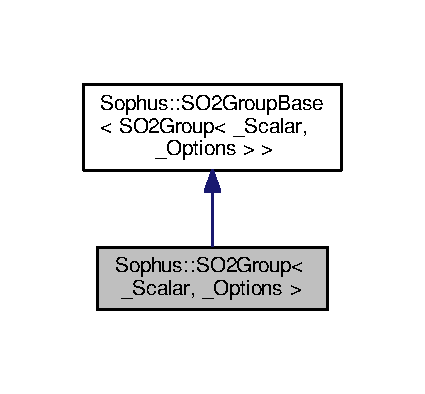
\includegraphics[width=204pt]{class_sophus_1_1_s_o2_group__inherit__graph}
\end{center}
\end{figure}


Collaboration diagram for Sophus\+:\+:S\+O2\+Group$<$ \+\_\+\+Scalar, \+\_\+\+Options $>$\+:
\nopagebreak
\begin{figure}[H]
\begin{center}
\leavevmode
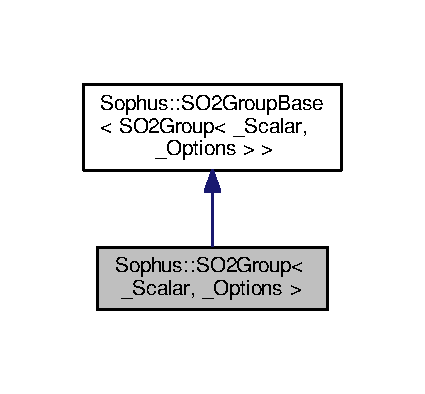
\includegraphics[width=204pt]{class_sophus_1_1_s_o2_group__coll__graph}
\end{center}
\end{figure}
\subsection*{Public Types}
\begin{DoxyCompactItemize}
\item 
typedef internal\+::traits$<$ \hyperlink{class_sophus_1_1_s_o2_group}{S\+O2\+Group}$<$ \+\_\+\+Scalar, \+\_\+\+Options $>$ $>$\+::\hyperlink{class_sophus_1_1_s_o2_group_a752943ea935a3007be93245ddd16bc74}{Scalar} \hyperlink{class_sophus_1_1_s_o2_group_a752943ea935a3007be93245ddd16bc74}{Scalar}\hypertarget{class_sophus_1_1_s_o2_group_a752943ea935a3007be93245ddd16bc74}{}\label{class_sophus_1_1_s_o2_group_a752943ea935a3007be93245ddd16bc74}

\begin{DoxyCompactList}\small\item\em scalar type \end{DoxyCompactList}\item 
typedef internal\+::traits$<$ \hyperlink{class_sophus_1_1_s_o2_group}{S\+O2\+Group}$<$ \+\_\+\+Scalar, \+\_\+\+Options $>$ $>$\+::Complex\+Type \& \hyperlink{class_sophus_1_1_s_o2_group_a2dc36b32ca3cec6727367d586d3263c6}{Complex\+Reference}\hypertarget{class_sophus_1_1_s_o2_group_a2dc36b32ca3cec6727367d586d3263c6}{}\label{class_sophus_1_1_s_o2_group_a2dc36b32ca3cec6727367d586d3263c6}

\begin{DoxyCompactList}\small\item\em complex number reference type \end{DoxyCompactList}\item 
typedef const internal\+::traits$<$ \hyperlink{class_sophus_1_1_s_o2_group}{S\+O2\+Group}$<$ \+\_\+\+Scalar, \+\_\+\+Options $>$ $>$\+::Complex\+Type \& \hyperlink{class_sophus_1_1_s_o2_group_a7d6e7964e8be6e4a79a6873382d2c996}{Const\+Complex\+Reference}\hypertarget{class_sophus_1_1_s_o2_group_a7d6e7964e8be6e4a79a6873382d2c996}{}\label{class_sophus_1_1_s_o2_group_a7d6e7964e8be6e4a79a6873382d2c996}

\begin{DoxyCompactList}\small\item\em complex number const reference type \end{DoxyCompactList}\item 
typedef \hyperlink{class_sophus_1_1_s_o2_group_base_a8981dccaf65802191e989815046b6a82}{Base\+::\+Transformation} \hyperlink{class_sophus_1_1_s_o2_group_a27d15c5fed370e583c258baf1abe8c62}{Transformation}\hypertarget{class_sophus_1_1_s_o2_group_a27d15c5fed370e583c258baf1abe8c62}{}\label{class_sophus_1_1_s_o2_group_a27d15c5fed370e583c258baf1abe8c62}

\begin{DoxyCompactList}\small\item\em group transfomation type \end{DoxyCompactList}\item 
typedef \hyperlink{class_sophus_1_1_s_o2_group_base_acdbb4a45d5f3d826b6bf8462c92c7f54}{Base\+::\+Point} \hyperlink{class_sophus_1_1_s_o2_group_ae27a57609394b29b56e4d2da2230262d}{Point}\hypertarget{class_sophus_1_1_s_o2_group_ae27a57609394b29b56e4d2da2230262d}{}\label{class_sophus_1_1_s_o2_group_ae27a57609394b29b56e4d2da2230262d}

\begin{DoxyCompactList}\small\item\em point type \end{DoxyCompactList}\item 
typedef \hyperlink{class_sophus_1_1_s_o2_group_base_a3701d07bf2791675518a0ceb33ce653b}{Base\+::\+Tangent} \hyperlink{class_sophus_1_1_s_o2_group_a1ae199a808bd3269e12061daddac3779}{Tangent}\hypertarget{class_sophus_1_1_s_o2_group_a1ae199a808bd3269e12061daddac3779}{}\label{class_sophus_1_1_s_o2_group_a1ae199a808bd3269e12061daddac3779}

\begin{DoxyCompactList}\small\item\em tangent vector type \end{DoxyCompactList}\item 
typedef \hyperlink{class_sophus_1_1_s_o2_group_base_a02b4843e52df827cf466eacd288697fa}{Base\+::\+Adjoint} \hyperlink{class_sophus_1_1_s_o2_group_abce282203ca280f7d1042f65040d29f3}{Adjoint}\hypertarget{class_sophus_1_1_s_o2_group_abce282203ca280f7d1042f65040d29f3}{}\label{class_sophus_1_1_s_o2_group_abce282203ca280f7d1042f65040d29f3}

\begin{DoxyCompactList}\small\item\em adjoint transformation type \end{DoxyCompactList}\end{DoxyCompactItemize}
\subsection*{Public Member Functions}
\begin{DoxyCompactItemize}
\item 
E\+I\+G\+E\+N\+\_\+\+M\+A\+K\+E\+\_\+\+A\+L\+I\+G\+N\+E\+D\+\_\+\+O\+P\+E\+R\+A\+T\+O\+R\+\_\+\+N\+EW \hyperlink{class_sophus_1_1_s_o2_group_a3d4158ae5cff1041b6b59822458d3936}{S\+O2\+Group} ()
\begin{DoxyCompactList}\small\item\em Default constructor. \end{DoxyCompactList}\item 
{\footnotesize template$<$typename Other\+Derived $>$ }\\\hyperlink{class_sophus_1_1_s_o2_group_a746020eda456033f97eec4df2068ed5e}{S\+O2\+Group} (const \hyperlink{class_sophus_1_1_s_o2_group_base}{S\+O2\+Group\+Base}$<$ Other\+Derived $>$ \&other)\hypertarget{class_sophus_1_1_s_o2_group_a746020eda456033f97eec4df2068ed5e}{}\label{class_sophus_1_1_s_o2_group_a746020eda456033f97eec4df2068ed5e}

\begin{DoxyCompactList}\small\item\em Copy constructor. \end{DoxyCompactList}\item 
\hyperlink{class_sophus_1_1_s_o2_group_a1f14c9f18b554399498515a7df008aa8}{S\+O2\+Group} (const \hyperlink{class_sophus_1_1_s_o2_group_a27d15c5fed370e583c258baf1abe8c62}{Transformation} \&R)
\begin{DoxyCompactList}\small\item\em Constructor from rotation matrix. \end{DoxyCompactList}\item 
\hyperlink{class_sophus_1_1_s_o2_group_a3c82efc2c592d1490ed150e1277bc59e}{S\+O2\+Group} (const \hyperlink{class_sophus_1_1_s_o2_group_a752943ea935a3007be93245ddd16bc74}{Scalar} \&real, const \hyperlink{class_sophus_1_1_s_o2_group_a752943ea935a3007be93245ddd16bc74}{Scalar} \&imag)
\begin{DoxyCompactList}\small\item\em Constructor from pair of real and imaginary number. \end{DoxyCompactList}\item 
\hyperlink{class_sophus_1_1_s_o2_group_a55aa0613418ec0e502308f8a7771008e}{S\+O2\+Group} (const Matrix$<$ \hyperlink{class_sophus_1_1_s_o2_group_a752943ea935a3007be93245ddd16bc74}{Scalar}, 2, 1 $>$ \&complex)
\begin{DoxyCompactList}\small\item\em Constructor from 2-\/vector. \end{DoxyCompactList}\item 
\hyperlink{class_sophus_1_1_s_o2_group_a44ebc87adef86623579747cf3cd24fa3}{S\+O2\+Group} (const std\+::complex$<$ \hyperlink{class_sophus_1_1_s_o2_group_a752943ea935a3007be93245ddd16bc74}{Scalar} $>$ \&complex)
\begin{DoxyCompactList}\small\item\em Constructor from std\+::complex. \end{DoxyCompactList}\item 
\hyperlink{class_sophus_1_1_s_o2_group_ad76cee9b273810bebc943494c5d6feed}{S\+O2\+Group} (\hyperlink{class_sophus_1_1_s_o2_group_a752943ea935a3007be93245ddd16bc74}{Scalar} theta)\hypertarget{class_sophus_1_1_s_o2_group_ad76cee9b273810bebc943494c5d6feed}{}\label{class_sophus_1_1_s_o2_group_ad76cee9b273810bebc943494c5d6feed}

\begin{DoxyCompactList}\small\item\em Constructor from an angle. \end{DoxyCompactList}\item 
E\+I\+G\+E\+N\+\_\+\+S\+T\+R\+O\+N\+G\+\_\+\+I\+N\+L\+I\+NE \hyperlink{class_sophus_1_1_s_o2_group_a7d6e7964e8be6e4a79a6873382d2c996}{Const\+Complex\+Reference} \hyperlink{class_sophus_1_1_s_o2_group_a96180bf3ec6c2935af72f94a6e8d700d}{unit\+\_\+complex} () const 
\begin{DoxyCompactList}\small\item\em Accessor of unit complex number. \end{DoxyCompactList}\end{DoxyCompactItemize}
\subsection*{Static Public Attributes}
\begin{DoxyCompactItemize}
\item 
static const int \hyperlink{class_sophus_1_1_s_o2_group_a849f639dd9eeb6a28f8c3b03f90ac4f4}{DoF} = Base\+::\+DoF\hypertarget{class_sophus_1_1_s_o2_group_a849f639dd9eeb6a28f8c3b03f90ac4f4}{}\label{class_sophus_1_1_s_o2_group_a849f639dd9eeb6a28f8c3b03f90ac4f4}

\begin{DoxyCompactList}\small\item\em degree of freedom of group \end{DoxyCompactList}\item 
static const int \hyperlink{class_sophus_1_1_s_o2_group_a80b788060cfccc5ae1cb3ff89abeb94e}{num\+\_\+parameters} = Base\+::num\+\_\+parameters\hypertarget{class_sophus_1_1_s_o2_group_a80b788060cfccc5ae1cb3ff89abeb94e}{}\label{class_sophus_1_1_s_o2_group_a80b788060cfccc5ae1cb3ff89abeb94e}

\begin{DoxyCompactList}\small\item\em number of internal parameters used \end{DoxyCompactList}\item 
static const int \hyperlink{class_sophus_1_1_s_o2_group_a356218141be974b71be760aa837caf11}{N} = Base\+::N\hypertarget{class_sophus_1_1_s_o2_group_a356218141be974b71be760aa837caf11}{}\label{class_sophus_1_1_s_o2_group_a356218141be974b71be760aa837caf11}

\begin{DoxyCompactList}\small\item\em group transformations are NxN matrices \end{DoxyCompactList}\end{DoxyCompactItemize}
\subsection*{Protected Member Functions}
\begin{DoxyCompactItemize}
\item 
E\+I\+G\+E\+N\+\_\+\+S\+T\+R\+O\+N\+G\+\_\+\+I\+N\+L\+I\+NE \hyperlink{class_sophus_1_1_s_o2_group_a2dc36b32ca3cec6727367d586d3263c6}{Complex\+Reference} {\bfseries unit\+\_\+complex\+\_\+nonconst} ()\hypertarget{class_sophus_1_1_s_o2_group_a3b44e6355030107733fc96cab4a31074}{}\label{class_sophus_1_1_s_o2_group_a3b44e6355030107733fc96cab4a31074}

\end{DoxyCompactItemize}
\subsection*{Static Protected Member Functions}
\begin{DoxyCompactItemize}
\item 
static bool {\bfseries is\+Near\+Zero} (const \hyperlink{class_sophus_1_1_s_o2_group_a752943ea935a3007be93245ddd16bc74}{Scalar} \&real, const \hyperlink{class_sophus_1_1_s_o2_group_a752943ea935a3007be93245ddd16bc74}{Scalar} \&imag)\hypertarget{class_sophus_1_1_s_o2_group_a92e753be12472d183b90e2723b199f3d}{}\label{class_sophus_1_1_s_o2_group_a92e753be12472d183b90e2723b199f3d}

\end{DoxyCompactItemize}
\subsection*{Protected Attributes}
\begin{DoxyCompactItemize}
\item 
Matrix$<$ \hyperlink{class_sophus_1_1_s_o2_group_a752943ea935a3007be93245ddd16bc74}{Scalar}, 2, 1 $>$ {\bfseries unit\+\_\+complex\+\_\+}\hypertarget{class_sophus_1_1_s_o2_group_ae1331f0c0cbe5b89b8ecec59f394204b}{}\label{class_sophus_1_1_s_o2_group_ae1331f0c0cbe5b89b8ecec59f394204b}

\end{DoxyCompactItemize}
\subsection*{Friends}
\begin{DoxyCompactItemize}
\item 
class {\bfseries S\+O2\+Group\+Base$<$ S\+O2\+Group$<$ \+\_\+\+Scalar, \+\_\+\+Options $>$ $>$}\hypertarget{class_sophus_1_1_s_o2_group_a6a116ef1b75da321cdd705e4e3e5e432}{}\label{class_sophus_1_1_s_o2_group_a6a116ef1b75da321cdd705e4e3e5e432}

\end{DoxyCompactItemize}
\subsection*{Additional Inherited Members}


\subsection{Detailed Description}
\subsubsection*{template$<$typename \+\_\+\+Scalar, int \+\_\+\+Options$>$\\*
class Sophus\+::\+S\+O2\+Group$<$ \+\_\+\+Scalar, \+\_\+\+Options $>$}

S\+O2 default type -\/ Constructors and default storage for S\+O2 Type. 

Definition at line 35 of file so2.\+hpp.



\subsection{Constructor \& Destructor Documentation}
\index{Sophus\+::\+S\+O2\+Group@{Sophus\+::\+S\+O2\+Group}!S\+O2\+Group@{S\+O2\+Group}}
\index{S\+O2\+Group@{S\+O2\+Group}!Sophus\+::\+S\+O2\+Group@{Sophus\+::\+S\+O2\+Group}}
\subsubsection[{\texorpdfstring{S\+O2\+Group()}{SO2Group()}}]{\setlength{\rightskip}{0pt plus 5cm}template$<$typename \+\_\+\+Scalar, int \+\_\+\+Options$>$ E\+I\+G\+E\+N\+\_\+\+M\+A\+K\+E\+\_\+\+A\+L\+I\+G\+N\+E\+D\+\_\+\+O\+P\+E\+R\+A\+T\+O\+R\+\_\+\+N\+EW {\bf Sophus\+::\+S\+O2\+Group}$<$ \+\_\+\+Scalar, \+\_\+\+Options $>$\+::{\bf S\+O2\+Group} (
\begin{DoxyParamCaption}
{}
\end{DoxyParamCaption}
)\hspace{0.3cm}{\ttfamily [inline]}}\hypertarget{class_sophus_1_1_s_o2_group_a3d4158ae5cff1041b6b59822458d3936}{}\label{class_sophus_1_1_s_o2_group_a3d4158ae5cff1041b6b59822458d3936}


Default constructor. 

Initialize complex number to identity rotation. 

Definition at line 474 of file so2.\+hpp.

\index{Sophus\+::\+S\+O2\+Group@{Sophus\+::\+S\+O2\+Group}!S\+O2\+Group@{S\+O2\+Group}}
\index{S\+O2\+Group@{S\+O2\+Group}!Sophus\+::\+S\+O2\+Group@{Sophus\+::\+S\+O2\+Group}}
\subsubsection[{\texorpdfstring{S\+O2\+Group(const Transformation \&\+R)}{SO2Group(const Transformation &R)}}]{\setlength{\rightskip}{0pt plus 5cm}template$<$typename \+\_\+\+Scalar, int \+\_\+\+Options$>$ {\bf Sophus\+::\+S\+O2\+Group}$<$ \+\_\+\+Scalar, \+\_\+\+Options $>$\+::{\bf S\+O2\+Group} (
\begin{DoxyParamCaption}
\item[{const {\bf Transformation} \&}]{R}
\end{DoxyParamCaption}
)\hspace{0.3cm}{\ttfamily [inline]}, {\ttfamily [explicit]}}\hypertarget{class_sophus_1_1_s_o2_group_a1f14c9f18b554399498515a7df008aa8}{}\label{class_sophus_1_1_s_o2_group_a1f14c9f18b554399498515a7df008aa8}


Constructor from rotation matrix. 

\begin{DoxyPrecond}{Precondition}
rotation matrix need to be orthogonal with determinant of 1 
\end{DoxyPrecond}


Definition at line 492 of file so2.\+hpp.

\index{Sophus\+::\+S\+O2\+Group@{Sophus\+::\+S\+O2\+Group}!S\+O2\+Group@{S\+O2\+Group}}
\index{S\+O2\+Group@{S\+O2\+Group}!Sophus\+::\+S\+O2\+Group@{Sophus\+::\+S\+O2\+Group}}
\subsubsection[{\texorpdfstring{S\+O2\+Group(const Scalar \&real, const Scalar \&imag)}{SO2Group(const Scalar &real, const Scalar &imag)}}]{\setlength{\rightskip}{0pt plus 5cm}template$<$typename \+\_\+\+Scalar, int \+\_\+\+Options$>$ {\bf Sophus\+::\+S\+O2\+Group}$<$ \+\_\+\+Scalar, \+\_\+\+Options $>$\+::{\bf S\+O2\+Group} (
\begin{DoxyParamCaption}
\item[{const {\bf Scalar} \&}]{real, }
\item[{const {\bf Scalar} \&}]{imag}
\end{DoxyParamCaption}
)\hspace{0.3cm}{\ttfamily [inline]}}\hypertarget{class_sophus_1_1_s_o2_group_a3c82efc2c592d1490ed150e1277bc59e}{}\label{class_sophus_1_1_s_o2_group_a3c82efc2c592d1490ed150e1277bc59e}


Constructor from pair of real and imaginary number. 

\begin{DoxyPrecond}{Precondition}
pair must not be zero 
\end{DoxyPrecond}


Definition at line 506 of file so2.\+hpp.

\index{Sophus\+::\+S\+O2\+Group@{Sophus\+::\+S\+O2\+Group}!S\+O2\+Group@{S\+O2\+Group}}
\index{S\+O2\+Group@{S\+O2\+Group}!Sophus\+::\+S\+O2\+Group@{Sophus\+::\+S\+O2\+Group}}
\subsubsection[{\texorpdfstring{S\+O2\+Group(const Matrix$<$ Scalar, 2, 1 $>$ \&complex)}{SO2Group(const Matrix< Scalar, 2, 1 > &complex)}}]{\setlength{\rightskip}{0pt plus 5cm}template$<$typename \+\_\+\+Scalar, int \+\_\+\+Options$>$ {\bf Sophus\+::\+S\+O2\+Group}$<$ \+\_\+\+Scalar, \+\_\+\+Options $>$\+::{\bf S\+O2\+Group} (
\begin{DoxyParamCaption}
\item[{const Matrix$<$ {\bf Scalar}, 2, 1 $>$ \&}]{complex}
\end{DoxyParamCaption}
)\hspace{0.3cm}{\ttfamily [inline]}, {\ttfamily [explicit]}}\hypertarget{class_sophus_1_1_s_o2_group_a55aa0613418ec0e502308f8a7771008e}{}\label{class_sophus_1_1_s_o2_group_a55aa0613418ec0e502308f8a7771008e}


Constructor from 2-\/vector. 

\begin{DoxyPrecond}{Precondition}
vector must not be zero 
\end{DoxyPrecond}


Definition at line 517 of file so2.\+hpp.

\index{Sophus\+::\+S\+O2\+Group@{Sophus\+::\+S\+O2\+Group}!S\+O2\+Group@{S\+O2\+Group}}
\index{S\+O2\+Group@{S\+O2\+Group}!Sophus\+::\+S\+O2\+Group@{Sophus\+::\+S\+O2\+Group}}
\subsubsection[{\texorpdfstring{S\+O2\+Group(const std\+::complex$<$ Scalar $>$ \&complex)}{SO2Group(const std::complex< Scalar > &complex)}}]{\setlength{\rightskip}{0pt plus 5cm}template$<$typename \+\_\+\+Scalar, int \+\_\+\+Options$>$ {\bf Sophus\+::\+S\+O2\+Group}$<$ \+\_\+\+Scalar, \+\_\+\+Options $>$\+::{\bf S\+O2\+Group} (
\begin{DoxyParamCaption}
\item[{const std\+::complex$<$ {\bf Scalar} $>$ \&}]{complex}
\end{DoxyParamCaption}
)\hspace{0.3cm}{\ttfamily [inline]}, {\ttfamily [explicit]}}\hypertarget{class_sophus_1_1_s_o2_group_a44ebc87adef86623579747cf3cd24fa3}{}\label{class_sophus_1_1_s_o2_group_a44ebc87adef86623579747cf3cd24fa3}


Constructor from std\+::complex. 

\begin{DoxyPrecond}{Precondition}
complex number must not be zero 
\end{DoxyPrecond}


Definition at line 528 of file so2.\+hpp.



\subsection{Member Function Documentation}
\index{Sophus\+::\+S\+O2\+Group@{Sophus\+::\+S\+O2\+Group}!unit\+\_\+complex@{unit\+\_\+complex}}
\index{unit\+\_\+complex@{unit\+\_\+complex}!Sophus\+::\+S\+O2\+Group@{Sophus\+::\+S\+O2\+Group}}
\subsubsection[{\texorpdfstring{unit\+\_\+complex() const }{unit_complex() const }}]{\setlength{\rightskip}{0pt plus 5cm}template$<$typename \+\_\+\+Scalar, int \+\_\+\+Options$>$ E\+I\+G\+E\+N\+\_\+\+S\+T\+R\+O\+N\+G\+\_\+\+I\+N\+L\+I\+NE {\bf Const\+Complex\+Reference} {\bf Sophus\+::\+S\+O2\+Group}$<$ \+\_\+\+Scalar, \+\_\+\+Options $>$\+::unit\+\_\+complex (
\begin{DoxyParamCaption}
{}
\end{DoxyParamCaption}
) const\hspace{0.3cm}{\ttfamily [inline]}}\hypertarget{class_sophus_1_1_s_o2_group_a96180bf3ec6c2935af72f94a6e8d700d}{}\label{class_sophus_1_1_s_o2_group_a96180bf3ec6c2935af72f94a6e8d700d}


Accessor of unit complex number. 

No direct write access is given to ensure the complex number stays normalized. 

Definition at line 548 of file so2.\+hpp.



The documentation for this class was generated from the following file\+:\begin{DoxyCompactItemize}
\item 
include/\+Sophus/sophus/so2.\+hpp\end{DoxyCompactItemize}

\hypertarget{class_sophus_1_1_s_o2_group_base}{}\section{Sophus\+:\+:S\+O2\+Group\+Base$<$ Derived $>$ Class Template Reference}
\label{class_sophus_1_1_s_o2_group_base}\index{Sophus\+::\+S\+O2\+Group\+Base$<$ Derived $>$@{Sophus\+::\+S\+O2\+Group\+Base$<$ Derived $>$}}


S\+O2 base type -\/ implements S\+O2 class but is storage agnostic.  




{\ttfamily \#include $<$so2.\+hpp$>$}



Inheritance diagram for Sophus\+:\+:S\+O2\+Group\+Base$<$ Derived $>$\+:
\nopagebreak
\begin{figure}[H]
\begin{center}
\leavevmode
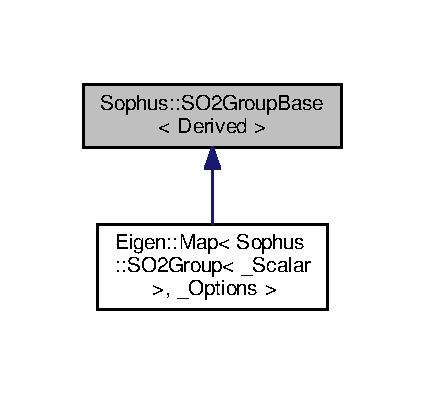
\includegraphics[width=204pt]{class_sophus_1_1_s_o2_group_base__inherit__graph}
\end{center}
\end{figure}
\subsection*{Public Types}
\begin{DoxyCompactItemize}
\item 
typedef internal\+::traits$<$ Derived $>$\+::\hyperlink{class_sophus_1_1_s_o2_group_base_a075b701502715aecf0bdb3464963d36c}{Scalar} \hyperlink{class_sophus_1_1_s_o2_group_base_a075b701502715aecf0bdb3464963d36c}{Scalar}\hypertarget{class_sophus_1_1_s_o2_group_base_a075b701502715aecf0bdb3464963d36c}{}\label{class_sophus_1_1_s_o2_group_base_a075b701502715aecf0bdb3464963d36c}

\begin{DoxyCompactList}\small\item\em scalar type \end{DoxyCompactList}\item 
typedef internal\+::traits$<$ Derived $>$\+::Complex\+Type \& \hyperlink{class_sophus_1_1_s_o2_group_base_adad5730f4c0387415b8dfc3c5aa8b8f2}{Complex\+Reference}\hypertarget{class_sophus_1_1_s_o2_group_base_adad5730f4c0387415b8dfc3c5aa8b8f2}{}\label{class_sophus_1_1_s_o2_group_base_adad5730f4c0387415b8dfc3c5aa8b8f2}

\begin{DoxyCompactList}\small\item\em complex number reference type \end{DoxyCompactList}\item 
typedef const internal\+::traits$<$ Derived $>$\+::Complex\+Type \& \hyperlink{class_sophus_1_1_s_o2_group_base_a077856f95a5c02933efd03aa1393825f}{Const\+Complex\+Reference}\hypertarget{class_sophus_1_1_s_o2_group_base_a077856f95a5c02933efd03aa1393825f}{}\label{class_sophus_1_1_s_o2_group_base_a077856f95a5c02933efd03aa1393825f}

\begin{DoxyCompactList}\small\item\em complex number const reference type \end{DoxyCompactList}\item 
typedef Matrix$<$ \hyperlink{class_sophus_1_1_s_o2_group_base_a075b701502715aecf0bdb3464963d36c}{Scalar}, \hyperlink{class_sophus_1_1_s_o2_group_base_ab6b062ff165cf8f3c3d8deb09ff4cf0e}{N}, \hyperlink{class_sophus_1_1_s_o2_group_base_ab6b062ff165cf8f3c3d8deb09ff4cf0e}{N} $>$ \hyperlink{class_sophus_1_1_s_o2_group_base_a8981dccaf65802191e989815046b6a82}{Transformation}\hypertarget{class_sophus_1_1_s_o2_group_base_a8981dccaf65802191e989815046b6a82}{}\label{class_sophus_1_1_s_o2_group_base_a8981dccaf65802191e989815046b6a82}

\begin{DoxyCompactList}\small\item\em group transfomation type \end{DoxyCompactList}\item 
typedef Matrix$<$ \hyperlink{class_sophus_1_1_s_o2_group_base_a075b701502715aecf0bdb3464963d36c}{Scalar}, 2, 1 $>$ \hyperlink{class_sophus_1_1_s_o2_group_base_acdbb4a45d5f3d826b6bf8462c92c7f54}{Point}\hypertarget{class_sophus_1_1_s_o2_group_base_acdbb4a45d5f3d826b6bf8462c92c7f54}{}\label{class_sophus_1_1_s_o2_group_base_acdbb4a45d5f3d826b6bf8462c92c7f54}

\begin{DoxyCompactList}\small\item\em point type \end{DoxyCompactList}\item 
typedef \hyperlink{class_sophus_1_1_s_o2_group_base_a075b701502715aecf0bdb3464963d36c}{Scalar} \hyperlink{class_sophus_1_1_s_o2_group_base_a3701d07bf2791675518a0ceb33ce653b}{Tangent}\hypertarget{class_sophus_1_1_s_o2_group_base_a3701d07bf2791675518a0ceb33ce653b}{}\label{class_sophus_1_1_s_o2_group_base_a3701d07bf2791675518a0ceb33ce653b}

\begin{DoxyCompactList}\small\item\em tangent vector type \end{DoxyCompactList}\item 
typedef \hyperlink{class_sophus_1_1_s_o2_group_base_a075b701502715aecf0bdb3464963d36c}{Scalar} \hyperlink{class_sophus_1_1_s_o2_group_base_a02b4843e52df827cf466eacd288697fa}{Adjoint}\hypertarget{class_sophus_1_1_s_o2_group_base_a02b4843e52df827cf466eacd288697fa}{}\label{class_sophus_1_1_s_o2_group_base_a02b4843e52df827cf466eacd288697fa}

\begin{DoxyCompactList}\small\item\em adjoint transformation type \end{DoxyCompactList}\end{DoxyCompactItemize}
\subsection*{Public Member Functions}
\begin{DoxyCompactItemize}
\item 
const \hyperlink{class_sophus_1_1_s_o2_group_base_a02b4843e52df827cf466eacd288697fa}{Adjoint} \hyperlink{class_sophus_1_1_s_o2_group_base_ada6ac17d59649f2c64ca5582c5e51d92}{Adj} () const 
\begin{DoxyCompactList}\small\item\em Adjoint transformation. \end{DoxyCompactList}\item 
{\footnotesize template$<$typename New\+Scalar\+Type $>$ }\\\hyperlink{class_sophus_1_1_s_o2_group}{S\+O2\+Group}$<$ New\+Scalar\+Type $>$ \hyperlink{class_sophus_1_1_s_o2_group_base_aa874d8841828cf62efd7e7c4a4f3b14b}{cast} () const 
\item 
\hyperlink{class_sophus_1_1_s_o2_group_base_a075b701502715aecf0bdb3464963d36c}{Scalar} $\ast$ \hyperlink{class_sophus_1_1_s_o2_group_base_ae9446146654e17b23bd9e0ec497461fb}{data} ()
\item 
const \hyperlink{class_sophus_1_1_s_o2_group_base_a075b701502715aecf0bdb3464963d36c}{Scalar} $\ast$ \hyperlink{class_sophus_1_1_s_o2_group_base_a2a86a713d9c6bce6aa285ec57d050249}{data} () const 
\item 
void \hyperlink{class_sophus_1_1_s_o2_group_base_ad00a8f66f8fc0814f395d92dcfb9943c}{fast\+Multiply} (const \hyperlink{class_sophus_1_1_s_o2_group}{S\+O2\+Group}$<$ \hyperlink{class_sophus_1_1_s_o2_group_base_a075b701502715aecf0bdb3464963d36c}{Scalar} $>$ \&other)
\begin{DoxyCompactList}\small\item\em Fast group multiplication. \end{DoxyCompactList}\item 
const \hyperlink{class_sophus_1_1_s_o2_group}{S\+O2\+Group}$<$ \hyperlink{class_sophus_1_1_s_o2_group_base_a075b701502715aecf0bdb3464963d36c}{Scalar} $>$ \hyperlink{class_sophus_1_1_s_o2_group_base_aa839d14832740111e954009345c9249b}{inverse} () const 
\item 
const \hyperlink{class_sophus_1_1_s_o2_group_base_a075b701502715aecf0bdb3464963d36c}{Scalar} \hyperlink{class_sophus_1_1_s_o2_group_base_a4663dc1acc7566b066125c900dc4beb1}{log} () const 
\begin{DoxyCompactList}\small\item\em Logarithmic map. \end{DoxyCompactList}\item 
void \hyperlink{class_sophus_1_1_s_o2_group_base_ab2012323b9b58e90e032ac4663225439}{normalize} ()
\begin{DoxyCompactList}\small\item\em Normalize complex number. \end{DoxyCompactList}\item 
const \hyperlink{class_sophus_1_1_s_o2_group_base_a8981dccaf65802191e989815046b6a82}{Transformation} \hyperlink{class_sophus_1_1_s_o2_group_base_a60e9726972a837a209cfcf6379ad17bf}{matrix} () const 
\item 
{\footnotesize template$<$typename Other\+Derived $>$ }\\\hyperlink{class_sophus_1_1_s_o2_group_base}{S\+O2\+Group\+Base}$<$ Derived $>$ \& \hyperlink{class_sophus_1_1_s_o2_group_base_a1fc0323f31179fb774417605b8296b3d}{operator=} (const \hyperlink{class_sophus_1_1_s_o2_group_base}{S\+O2\+Group\+Base}$<$ Other\+Derived $>$ \&other)\hypertarget{class_sophus_1_1_s_o2_group_base_a1fc0323f31179fb774417605b8296b3d}{}\label{class_sophus_1_1_s_o2_group_base_a1fc0323f31179fb774417605b8296b3d}

\begin{DoxyCompactList}\small\item\em Assignment operator. \end{DoxyCompactList}\item 
const \hyperlink{class_sophus_1_1_s_o2_group}{S\+O2\+Group}$<$ \hyperlink{class_sophus_1_1_s_o2_group_base_a075b701502715aecf0bdb3464963d36c}{Scalar} $>$ \hyperlink{class_sophus_1_1_s_o2_group_base_a7afe754a865b880bb6f3c69836512e3d}{operator$\ast$} (const \hyperlink{class_sophus_1_1_s_o2_group}{S\+O2\+Group}$<$ \hyperlink{class_sophus_1_1_s_o2_group_base_a075b701502715aecf0bdb3464963d36c}{Scalar} $>$ \&other) const 
\begin{DoxyCompactList}\small\item\em Group multiplication. \end{DoxyCompactList}\item 
const \hyperlink{class_sophus_1_1_s_o2_group_base_acdbb4a45d5f3d826b6bf8462c92c7f54}{Point} \hyperlink{class_sophus_1_1_s_o2_group_base_a414ff89adc6822ad330a0c9e2694c420}{operator$\ast$} (const \hyperlink{class_sophus_1_1_s_o2_group_base_acdbb4a45d5f3d826b6bf8462c92c7f54}{Point} \&p) const 
\begin{DoxyCompactList}\small\item\em Group action on $ \mathbf{R}^2 $. \end{DoxyCompactList}\item 
void \hyperlink{class_sophus_1_1_s_o2_group_base_a68b1cf84a0e585432508e5310df677db}{operator$\ast$=} (const \hyperlink{class_sophus_1_1_s_o2_group}{S\+O2\+Group}$<$ \hyperlink{class_sophus_1_1_s_o2_group_base_a075b701502715aecf0bdb3464963d36c}{Scalar} $>$ \&other)
\begin{DoxyCompactList}\small\item\em In-\/place group multiplication. \end{DoxyCompactList}\item 
void \hyperlink{class_sophus_1_1_s_o2_group_base_afc649b78e35d2a7504a88002a978b8b9}{set\+Complex} (const \hyperlink{class_sophus_1_1_s_o2_group_base_acdbb4a45d5f3d826b6bf8462c92c7f54}{Point} \&complex)
\begin{DoxyCompactList}\small\item\em Setter of internal unit complex number representation. \end{DoxyCompactList}\item 
E\+I\+G\+E\+N\+\_\+\+S\+T\+R\+O\+N\+G\+\_\+\+I\+N\+L\+I\+NE \hyperlink{class_sophus_1_1_s_o2_group_base_a077856f95a5c02933efd03aa1393825f}{Const\+Complex\+Reference} \hyperlink{class_sophus_1_1_s_o2_group_base_a36a0a9344d5639ddc85a40bc0f4fee8b}{unit\+\_\+complex} () const 
\begin{DoxyCompactList}\small\item\em Accessor of unit complex number. \end{DoxyCompactList}\end{DoxyCompactItemize}
\subsection*{Static Public Member Functions}
\begin{DoxyCompactItemize}
\item 
static const \hyperlink{class_sophus_1_1_s_o2_group}{S\+O2\+Group}$<$ \hyperlink{class_sophus_1_1_s_o2_group_base_a075b701502715aecf0bdb3464963d36c}{Scalar} $>$ \hyperlink{class_sophus_1_1_s_o2_group_base_ab2f306cce273dddb1dff74bc4156e0a8}{exp} (const \hyperlink{class_sophus_1_1_s_o2_group_base_a3701d07bf2791675518a0ceb33ce653b}{Tangent} \&theta)
\begin{DoxyCompactList}\small\item\em Group exponential. \end{DoxyCompactList}\item 
static const \hyperlink{class_sophus_1_1_s_o2_group_base_a8981dccaf65802191e989815046b6a82}{Transformation} \hyperlink{class_sophus_1_1_s_o2_group_base_ac843066964e2fd31ad1fa7fe07d6f256}{generator} ()
\begin{DoxyCompactList}\small\item\em Generator. \end{DoxyCompactList}\item 
static const \hyperlink{class_sophus_1_1_s_o2_group_base_a8981dccaf65802191e989815046b6a82}{Transformation} \hyperlink{class_sophus_1_1_s_o2_group_base_a9f87c5799f00e799f8087f786389cb13}{hat} (const \hyperlink{class_sophus_1_1_s_o2_group_base_a3701d07bf2791675518a0ceb33ce653b}{Tangent} \&theta)
\begin{DoxyCompactList}\small\item\em hat-\/operator \end{DoxyCompactList}\item 
static const \hyperlink{class_sophus_1_1_s_o2_group_base_a3701d07bf2791675518a0ceb33ce653b}{Tangent} \hyperlink{class_sophus_1_1_s_o2_group_base_a009f4077e6fc4db7e0e4e011e084ff12}{lie\+Bracket} (const \hyperlink{class_sophus_1_1_s_o2_group_base_a3701d07bf2791675518a0ceb33ce653b}{Tangent} \&theta1, const \hyperlink{class_sophus_1_1_s_o2_group_base_a3701d07bf2791675518a0ceb33ce653b}{Tangent} \&theta2)
\begin{DoxyCompactList}\small\item\em Lie bracket. \end{DoxyCompactList}\item 
static const \hyperlink{class_sophus_1_1_s_o2_group_base_a3701d07bf2791675518a0ceb33ce653b}{Tangent} \hyperlink{class_sophus_1_1_s_o2_group_base_a5a64721b7036cd64c6d64a1880b111e3}{log} (const \hyperlink{class_sophus_1_1_s_o2_group}{S\+O2\+Group}$<$ \hyperlink{class_sophus_1_1_s_o2_group_base_a075b701502715aecf0bdb3464963d36c}{Scalar} $>$ \&other)
\begin{DoxyCompactList}\small\item\em Logarithmic map. \end{DoxyCompactList}\item 
static const \hyperlink{class_sophus_1_1_s_o2_group_base_a3701d07bf2791675518a0ceb33ce653b}{Tangent} \hyperlink{class_sophus_1_1_s_o2_group_base_a08d1bf2d8cd13cd07734f67963d7fd16}{vee} (const \hyperlink{class_sophus_1_1_s_o2_group_base_a8981dccaf65802191e989815046b6a82}{Transformation} \&Omega)
\begin{DoxyCompactList}\small\item\em vee-\/operator \end{DoxyCompactList}\end{DoxyCompactItemize}
\subsection*{Static Public Attributes}
\begin{DoxyCompactItemize}
\item 
static const int \hyperlink{class_sophus_1_1_s_o2_group_base_aece4b1b66a60eee58224b3a89b8f47b1}{DoF} = 1\hypertarget{class_sophus_1_1_s_o2_group_base_aece4b1b66a60eee58224b3a89b8f47b1}{}\label{class_sophus_1_1_s_o2_group_base_aece4b1b66a60eee58224b3a89b8f47b1}

\begin{DoxyCompactList}\small\item\em degree of freedom of group (one for in-\/plane rotation) \end{DoxyCompactList}\item 
static const int \hyperlink{class_sophus_1_1_s_o2_group_base_a05f97013bff73cc09cdcaea0b2693664}{num\+\_\+parameters} = 2\hypertarget{class_sophus_1_1_s_o2_group_base_a05f97013bff73cc09cdcaea0b2693664}{}\label{class_sophus_1_1_s_o2_group_base_a05f97013bff73cc09cdcaea0b2693664}

\begin{DoxyCompactList}\small\item\em number of internal parameters used (unit complex number for rotation) \end{DoxyCompactList}\item 
static const int \hyperlink{class_sophus_1_1_s_o2_group_base_ab6b062ff165cf8f3c3d8deb09ff4cf0e}{N} = 2\hypertarget{class_sophus_1_1_s_o2_group_base_ab6b062ff165cf8f3c3d8deb09ff4cf0e}{}\label{class_sophus_1_1_s_o2_group_base_ab6b062ff165cf8f3c3d8deb09ff4cf0e}

\begin{DoxyCompactList}\small\item\em group transformations are NxN matrices \end{DoxyCompactList}\end{DoxyCompactItemize}


\subsection{Detailed Description}
\subsubsection*{template$<$typename Derived$>$\\*
class Sophus\+::\+S\+O2\+Group\+Base$<$ Derived $>$}

S\+O2 base type -\/ implements S\+O2 class but is storage agnostic. 

\mbox{[}add more detailed description/tutorial\mbox{]} 

Definition at line 84 of file so2.\+hpp.



\subsection{Member Function Documentation}
\index{Sophus\+::\+S\+O2\+Group\+Base@{Sophus\+::\+S\+O2\+Group\+Base}!Adj@{Adj}}
\index{Adj@{Adj}!Sophus\+::\+S\+O2\+Group\+Base@{Sophus\+::\+S\+O2\+Group\+Base}}
\subsubsection[{\texorpdfstring{Adj() const }{Adj() const }}]{\setlength{\rightskip}{0pt plus 5cm}template$<$typename Derived$>$ const {\bf Adjoint} {\bf Sophus\+::\+S\+O2\+Group\+Base}$<$ Derived $>$\+::Adj (
\begin{DoxyParamCaption}
{}
\end{DoxyParamCaption}
) const\hspace{0.3cm}{\ttfamily [inline]}}\hypertarget{class_sophus_1_1_s_o2_group_base_ada6ac17d59649f2c64ca5582c5e51d92}{}\label{class_sophus_1_1_s_o2_group_base_ada6ac17d59649f2c64ca5582c5e51d92}


Adjoint transformation. 

This function return the adjoint transformation $ Ad $ of the group instance $ A $ such that for all $ x $ it holds that $ \widehat{Ad_A\cdot x} = A\widehat{x}A^{-1} $ with $\ \widehat{\cdot} $ being the \hyperlink{class_sophus_1_1_s_o2_group_base_a9f87c5799f00e799f8087f786389cb13}{hat()}-\/operator.

For S\+O2, it simply returns 1. 

Definition at line 123 of file so2.\+hpp.

\index{Sophus\+::\+S\+O2\+Group\+Base@{Sophus\+::\+S\+O2\+Group\+Base}!cast@{cast}}
\index{cast@{cast}!Sophus\+::\+S\+O2\+Group\+Base@{Sophus\+::\+S\+O2\+Group\+Base}}
\subsubsection[{\texorpdfstring{cast() const }{cast() const }}]{\setlength{\rightskip}{0pt plus 5cm}template$<$typename Derived$>$ template$<$typename New\+Scalar\+Type $>$ {\bf S\+O2\+Group}$<$New\+Scalar\+Type$>$ {\bf Sophus\+::\+S\+O2\+Group\+Base}$<$ Derived $>$\+::cast (
\begin{DoxyParamCaption}
{}
\end{DoxyParamCaption}
) const\hspace{0.3cm}{\ttfamily [inline]}}\hypertarget{class_sophus_1_1_s_o2_group_base_aa874d8841828cf62efd7e7c4a4f3b14b}{}\label{class_sophus_1_1_s_o2_group_base_aa874d8841828cf62efd7e7c4a4f3b14b}
\begin{DoxyReturn}{Returns}
copy of instance casted to New\+Scalar\+Type 
\end{DoxyReturn}


Definition at line 131 of file so2.\+hpp.

\index{Sophus\+::\+S\+O2\+Group\+Base@{Sophus\+::\+S\+O2\+Group\+Base}!data@{data}}
\index{data@{data}!Sophus\+::\+S\+O2\+Group\+Base@{Sophus\+::\+S\+O2\+Group\+Base}}
\subsubsection[{\texorpdfstring{data()}{data()}}]{\setlength{\rightskip}{0pt plus 5cm}template$<$typename Derived$>$ {\bf Scalar}$\ast$ {\bf Sophus\+::\+S\+O2\+Group\+Base}$<$ Derived $>$\+::data (
\begin{DoxyParamCaption}
{}
\end{DoxyParamCaption}
)\hspace{0.3cm}{\ttfamily [inline]}}\hypertarget{class_sophus_1_1_s_o2_group_base_ae9446146654e17b23bd9e0ec497461fb}{}\label{class_sophus_1_1_s_o2_group_base_ae9446146654e17b23bd9e0ec497461fb}
\begin{DoxyReturn}{Returns}
pointer to internal data
\end{DoxyReturn}
This provides unsafe read/write access to internal data. S\+O2 is represented by a complex number with unit length (two parameters). When using direct write access, the user needs to take care of that the complex number stays normalized.

\begin{DoxySeeAlso}{See also}
\hyperlink{class_sophus_1_1_s_o2_group_base_ab2012323b9b58e90e032ac4663225439}{normalize()} 
\end{DoxySeeAlso}


Definition at line 146 of file so2.\+hpp.

\index{Sophus\+::\+S\+O2\+Group\+Base@{Sophus\+::\+S\+O2\+Group\+Base}!data@{data}}
\index{data@{data}!Sophus\+::\+S\+O2\+Group\+Base@{Sophus\+::\+S\+O2\+Group\+Base}}
\subsubsection[{\texorpdfstring{data() const }{data() const }}]{\setlength{\rightskip}{0pt plus 5cm}template$<$typename Derived$>$ const {\bf Scalar}$\ast$ {\bf Sophus\+::\+S\+O2\+Group\+Base}$<$ Derived $>$\+::data (
\begin{DoxyParamCaption}
{}
\end{DoxyParamCaption}
) const\hspace{0.3cm}{\ttfamily [inline]}}\hypertarget{class_sophus_1_1_s_o2_group_base_a2a86a713d9c6bce6aa285ec57d050249}{}\label{class_sophus_1_1_s_o2_group_base_a2a86a713d9c6bce6aa285ec57d050249}
\begin{DoxyReturn}{Returns}
const pointer to internal data
\end{DoxyReturn}
Const version of \hyperlink{class_sophus_1_1_s_o2_group_base_ae9446146654e17b23bd9e0ec497461fb}{data()}. 

Definition at line 155 of file so2.\+hpp.

\index{Sophus\+::\+S\+O2\+Group\+Base@{Sophus\+::\+S\+O2\+Group\+Base}!exp@{exp}}
\index{exp@{exp}!Sophus\+::\+S\+O2\+Group\+Base@{Sophus\+::\+S\+O2\+Group\+Base}}
\subsubsection[{\texorpdfstring{exp(const Tangent \&theta)}{exp(const Tangent &theta)}}]{\setlength{\rightskip}{0pt plus 5cm}template$<$typename Derived$>$ static const {\bf S\+O2\+Group}$<${\bf Scalar}$>$ {\bf Sophus\+::\+S\+O2\+Group\+Base}$<$ Derived $>$\+::exp (
\begin{DoxyParamCaption}
\item[{const {\bf Tangent} \&}]{theta}
\end{DoxyParamCaption}
)\hspace{0.3cm}{\ttfamily [inline]}, {\ttfamily [static]}}\hypertarget{class_sophus_1_1_s_o2_group_base_ab2f306cce273dddb1dff74bc4156e0a8}{}\label{class_sophus_1_1_s_o2_group_base_ab2f306cce273dddb1dff74bc4156e0a8}


Group exponential. 


\begin{DoxyParams}{Parameters}
{\em theta} & tangent space element (=rotation angle $ \theta $) \\
\hline
\end{DoxyParams}
\begin{DoxyReturn}{Returns}
corresponding element of the group S\+O2
\end{DoxyReturn}
To be more specific, this function computes $ \exp(\widehat{\theta}) $ with $ \exp(\cdot) $ being the matrix exponential and $ \widehat{\cdot} $ the \hyperlink{class_sophus_1_1_s_o2_group_base_a9f87c5799f00e799f8087f786389cb13}{hat()}-\/operator of S\+O2.

\begin{DoxySeeAlso}{See also}
\hyperlink{class_sophus_1_1_s_o2_group_base_a9f87c5799f00e799f8087f786389cb13}{hat()} 

\hyperlink{class_sophus_1_1_s_o2_group_base_a4663dc1acc7566b066125c900dc4beb1}{log()} 
\end{DoxySeeAlso}


Definition at line 322 of file so2.\+hpp.

\index{Sophus\+::\+S\+O2\+Group\+Base@{Sophus\+::\+S\+O2\+Group\+Base}!fast\+Multiply@{fast\+Multiply}}
\index{fast\+Multiply@{fast\+Multiply}!Sophus\+::\+S\+O2\+Group\+Base@{Sophus\+::\+S\+O2\+Group\+Base}}
\subsubsection[{\texorpdfstring{fast\+Multiply(const S\+O2\+Group$<$ Scalar $>$ \&other)}{fastMultiply(const SO2Group< Scalar > &other)}}]{\setlength{\rightskip}{0pt plus 5cm}template$<$typename Derived$>$ void {\bf Sophus\+::\+S\+O2\+Group\+Base}$<$ Derived $>$\+::fast\+Multiply (
\begin{DoxyParamCaption}
\item[{const {\bf S\+O2\+Group}$<$ {\bf Scalar} $>$ \&}]{other}
\end{DoxyParamCaption}
)\hspace{0.3cm}{\ttfamily [inline]}}\hypertarget{class_sophus_1_1_s_o2_group_base_ad00a8f66f8fc0814f395d92dcfb9943c}{}\label{class_sophus_1_1_s_o2_group_base_ad00a8f66f8fc0814f395d92dcfb9943c}


Fast group multiplication. 

This method is a fast version of \hyperlink{class_sophus_1_1_s_o2_group_base_a68b1cf84a0e585432508e5310df677db}{operator$\ast$=()}, since it does not perform normalization. It is up to the user to call \hyperlink{class_sophus_1_1_s_o2_group_base_ab2012323b9b58e90e032ac4663225439}{normalize()} once in a while.

\begin{DoxySeeAlso}{See also}
\hyperlink{class_sophus_1_1_s_o2_group_base_a68b1cf84a0e585432508e5310df677db}{operator$\ast$=()} 
\end{DoxySeeAlso}


Definition at line 168 of file so2.\+hpp.

\index{Sophus\+::\+S\+O2\+Group\+Base@{Sophus\+::\+S\+O2\+Group\+Base}!generator@{generator}}
\index{generator@{generator}!Sophus\+::\+S\+O2\+Group\+Base@{Sophus\+::\+S\+O2\+Group\+Base}}
\subsubsection[{\texorpdfstring{generator()}{generator()}}]{\setlength{\rightskip}{0pt plus 5cm}template$<$typename Derived$>$ static const {\bf Transformation} {\bf Sophus\+::\+S\+O2\+Group\+Base}$<$ Derived $>$\+::generator (
\begin{DoxyParamCaption}
{}
\end{DoxyParamCaption}
)\hspace{0.3cm}{\ttfamily [inline]}, {\ttfamily [static]}}\hypertarget{class_sophus_1_1_s_o2_group_base_ac843066964e2fd31ad1fa7fe07d6f256}{}\label{class_sophus_1_1_s_o2_group_base_ac843066964e2fd31ad1fa7fe07d6f256}


Generator. 

The infinitesimal generator of S\+O2 is $ G_0 = \left( \begin{array}{ccc} 0& -1& \\ 1& 0& \end{array} \right). $ \begin{DoxySeeAlso}{See also}
\hyperlink{class_sophus_1_1_s_o2_group_base_a9f87c5799f00e799f8087f786389cb13}{hat()} 
\end{DoxySeeAlso}


Definition at line 339 of file so2.\+hpp.

\index{Sophus\+::\+S\+O2\+Group\+Base@{Sophus\+::\+S\+O2\+Group\+Base}!hat@{hat}}
\index{hat@{hat}!Sophus\+::\+S\+O2\+Group\+Base@{Sophus\+::\+S\+O2\+Group\+Base}}
\subsubsection[{\texorpdfstring{hat(const Tangent \&theta)}{hat(const Tangent &theta)}}]{\setlength{\rightskip}{0pt plus 5cm}template$<$typename Derived$>$ static const {\bf Transformation} {\bf Sophus\+::\+S\+O2\+Group\+Base}$<$ Derived $>$\+::hat (
\begin{DoxyParamCaption}
\item[{const {\bf Tangent} \&}]{theta}
\end{DoxyParamCaption}
)\hspace{0.3cm}{\ttfamily [inline]}, {\ttfamily [static]}}\hypertarget{class_sophus_1_1_s_o2_group_base_a9f87c5799f00e799f8087f786389cb13}{}\label{class_sophus_1_1_s_o2_group_base_a9f87c5799f00e799f8087f786389cb13}


hat-\/operator 


\begin{DoxyParams}{Parameters}
{\em theta} & scalar representation of Lie algebra element \\
\hline
\end{DoxyParams}
\begin{DoxyReturn}{Returns}
2x2-\/matrix representatin of Lie algebra element
\end{DoxyReturn}
Formally, the hat-\/operator of S\+O2 is defined as $ \widehat{\cdot}: \mathbf{R}^2 \rightarrow \mathbf{R}^{2\times 2}, \quad \widehat{\theta} = G_0\cdot \theta $ with $ G_0 $ being the infinitesial \hyperlink{class_sophus_1_1_s_o2_group_base_ac843066964e2fd31ad1fa7fe07d6f256}{generator()}.

\begin{DoxySeeAlso}{See also}
\hyperlink{class_sophus_1_1_s_o2_group_base_ac843066964e2fd31ad1fa7fe07d6f256}{generator()} 

\hyperlink{class_sophus_1_1_s_o2_group_base_a08d1bf2d8cd13cd07734f67963d7fd16}{vee()} 
\end{DoxySeeAlso}


Definition at line 358 of file so2.\+hpp.

\index{Sophus\+::\+S\+O2\+Group\+Base@{Sophus\+::\+S\+O2\+Group\+Base}!inverse@{inverse}}
\index{inverse@{inverse}!Sophus\+::\+S\+O2\+Group\+Base@{Sophus\+::\+S\+O2\+Group\+Base}}
\subsubsection[{\texorpdfstring{inverse() const }{inverse() const }}]{\setlength{\rightskip}{0pt plus 5cm}template$<$typename Derived$>$ const {\bf S\+O2\+Group}$<${\bf Scalar}$>$ {\bf Sophus\+::\+S\+O2\+Group\+Base}$<$ Derived $>$\+::inverse (
\begin{DoxyParamCaption}
{}
\end{DoxyParamCaption}
) const\hspace{0.3cm}{\ttfamily [inline]}}\hypertarget{class_sophus_1_1_s_o2_group_base_aa839d14832740111e954009345c9249b}{}\label{class_sophus_1_1_s_o2_group_base_aa839d14832740111e954009345c9249b}
\begin{DoxyReturn}{Returns}
group inverse of instance 
\end{DoxyReturn}


Definition at line 182 of file so2.\+hpp.

\index{Sophus\+::\+S\+O2\+Group\+Base@{Sophus\+::\+S\+O2\+Group\+Base}!lie\+Bracket@{lie\+Bracket}}
\index{lie\+Bracket@{lie\+Bracket}!Sophus\+::\+S\+O2\+Group\+Base@{Sophus\+::\+S\+O2\+Group\+Base}}
\subsubsection[{\texorpdfstring{lie\+Bracket(const Tangent \&theta1, const Tangent \&theta2)}{lieBracket(const Tangent &theta1, const Tangent &theta2)}}]{\setlength{\rightskip}{0pt plus 5cm}template$<$typename Derived$>$ static const {\bf Tangent} {\bf Sophus\+::\+S\+O2\+Group\+Base}$<$ Derived $>$\+::lie\+Bracket (
\begin{DoxyParamCaption}
\item[{const {\bf Tangent} \&}]{theta1, }
\item[{const {\bf Tangent} \&}]{theta2}
\end{DoxyParamCaption}
)\hspace{0.3cm}{\ttfamily [inline]}, {\ttfamily [static]}}\hypertarget{class_sophus_1_1_s_o2_group_base_a009f4077e6fc4db7e0e4e011e084ff12}{}\label{class_sophus_1_1_s_o2_group_base_a009f4077e6fc4db7e0e4e011e084ff12}


Lie bracket. 


\begin{DoxyParams}{Parameters}
{\em theta1} & scalar representation of Lie algebra element \\
\hline
{\em theta2} & scalar representation of Lie algebra element \\
\hline
\end{DoxyParams}
\begin{DoxyReturn}{Returns}
zero
\end{DoxyReturn}
It computes the bracket. For the Lie algebra so2, the Lie bracket is simply $ [\theta_1, \theta_2]_{so2} = 0 $ since S\+O2 is a commutative group.

\begin{DoxySeeAlso}{See also}
\hyperlink{class_sophus_1_1_s_o2_group_base_a9f87c5799f00e799f8087f786389cb13}{hat()} 

\hyperlink{class_sophus_1_1_s_o2_group_base_a08d1bf2d8cd13cd07734f67963d7fd16}{vee()} 
\end{DoxySeeAlso}


Definition at line 380 of file so2.\+hpp.

\index{Sophus\+::\+S\+O2\+Group\+Base@{Sophus\+::\+S\+O2\+Group\+Base}!log@{log}}
\index{log@{log}!Sophus\+::\+S\+O2\+Group\+Base@{Sophus\+::\+S\+O2\+Group\+Base}}
\subsubsection[{\texorpdfstring{log() const }{log() const }}]{\setlength{\rightskip}{0pt plus 5cm}template$<$typename Derived$>$ const {\bf Scalar} {\bf Sophus\+::\+S\+O2\+Group\+Base}$<$ Derived $>$\+::log (
\begin{DoxyParamCaption}
{}
\end{DoxyParamCaption}
) const\hspace{0.3cm}{\ttfamily [inline]}}\hypertarget{class_sophus_1_1_s_o2_group_base_a4663dc1acc7566b066125c900dc4beb1}{}\label{class_sophus_1_1_s_o2_group_base_a4663dc1acc7566b066125c900dc4beb1}


Logarithmic map. 

\begin{DoxyReturn}{Returns}
tangent space representation (=rotation angle) of instance
\end{DoxyReturn}
\begin{DoxySeeAlso}{See also}
\hyperlink{class_sophus_1_1_s_o2_group_base_a4663dc1acc7566b066125c900dc4beb1}{log()}. 
\end{DoxySeeAlso}


Definition at line 194 of file so2.\+hpp.

\index{Sophus\+::\+S\+O2\+Group\+Base@{Sophus\+::\+S\+O2\+Group\+Base}!log@{log}}
\index{log@{log}!Sophus\+::\+S\+O2\+Group\+Base@{Sophus\+::\+S\+O2\+Group\+Base}}
\subsubsection[{\texorpdfstring{log(const S\+O2\+Group$<$ Scalar $>$ \&other)}{log(const SO2Group< Scalar > &other)}}]{\setlength{\rightskip}{0pt plus 5cm}template$<$typename Derived$>$ static const {\bf Tangent} {\bf Sophus\+::\+S\+O2\+Group\+Base}$<$ Derived $>$\+::log (
\begin{DoxyParamCaption}
\item[{const {\bf S\+O2\+Group}$<$ {\bf Scalar} $>$ \&}]{other}
\end{DoxyParamCaption}
)\hspace{0.3cm}{\ttfamily [inline]}, {\ttfamily [static]}}\hypertarget{class_sophus_1_1_s_o2_group_base_a5a64721b7036cd64c6d64a1880b111e3}{}\label{class_sophus_1_1_s_o2_group_base_a5a64721b7036cd64c6d64a1880b111e3}


Logarithmic map. 


\begin{DoxyParams}{Parameters}
{\em other} & element of the group S\+O2 \\
\hline
\end{DoxyParams}
\begin{DoxyReturn}{Returns}
corresponding tangent space element (=rotation angle $ \theta $)
\end{DoxyReturn}
Computes the logarithmic, the inverse of the group exponential. To be specific, this function computes $ \log({\cdot})^\vee $ with $ \vee(\cdot) $ being the matrix logarithm and $ \vee{\cdot} $ the \hyperlink{class_sophus_1_1_s_o2_group_base_a08d1bf2d8cd13cd07734f67963d7fd16}{vee()}-\/operator of S\+O2.

\begin{DoxySeeAlso}{See also}
\hyperlink{class_sophus_1_1_s_o2_group_base_ab2f306cce273dddb1dff74bc4156e0a8}{exp()} 

\hyperlink{class_sophus_1_1_s_o2_group_base_a08d1bf2d8cd13cd07734f67963d7fd16}{vee()} 
\end{DoxySeeAlso}


Definition at line 401 of file so2.\+hpp.

\index{Sophus\+::\+S\+O2\+Group\+Base@{Sophus\+::\+S\+O2\+Group\+Base}!matrix@{matrix}}
\index{matrix@{matrix}!Sophus\+::\+S\+O2\+Group\+Base@{Sophus\+::\+S\+O2\+Group\+Base}}
\subsubsection[{\texorpdfstring{matrix() const }{matrix() const }}]{\setlength{\rightskip}{0pt plus 5cm}template$<$typename Derived$>$ const {\bf Transformation} {\bf Sophus\+::\+S\+O2\+Group\+Base}$<$ Derived $>$\+::matrix (
\begin{DoxyParamCaption}
{}
\end{DoxyParamCaption}
) const\hspace{0.3cm}{\ttfamily [inline]}}\hypertarget{class_sophus_1_1_s_o2_group_base_a60e9726972a837a209cfcf6379ad17bf}{}\label{class_sophus_1_1_s_o2_group_base_a60e9726972a837a209cfcf6379ad17bf}
\begin{DoxyReturn}{Returns}
2x2 matrix representation of instance
\end{DoxyReturn}
For S\+O2, the matrix representation is an orthogonal matrix R with det(\+R)=1, thus the so-\/called rotation matrix. 

Definition at line 223 of file so2.\+hpp.

\index{Sophus\+::\+S\+O2\+Group\+Base@{Sophus\+::\+S\+O2\+Group\+Base}!normalize@{normalize}}
\index{normalize@{normalize}!Sophus\+::\+S\+O2\+Group\+Base@{Sophus\+::\+S\+O2\+Group\+Base}}
\subsubsection[{\texorpdfstring{normalize()}{normalize()}}]{\setlength{\rightskip}{0pt plus 5cm}template$<$typename Derived$>$ void {\bf Sophus\+::\+S\+O2\+Group\+Base}$<$ Derived $>$\+::normalize (
\begin{DoxyParamCaption}
{}
\end{DoxyParamCaption}
)\hspace{0.3cm}{\ttfamily [inline]}}\hypertarget{class_sophus_1_1_s_o2_group_base_ab2012323b9b58e90e032ac4663225439}{}\label{class_sophus_1_1_s_o2_group_base_ab2012323b9b58e90e032ac4663225439}


Normalize complex number. 

It re-\/normalizes complex number to unit length. This method only needs to be called in conjunction with \hyperlink{class_sophus_1_1_s_o2_group_base_ad00a8f66f8fc0814f395d92dcfb9943c}{fast\+Multiply()} or \hyperlink{class_sophus_1_1_s_o2_group_base_ae9446146654e17b23bd9e0ec497461fb}{data()} write access. 

Definition at line 205 of file so2.\+hpp.

\index{Sophus\+::\+S\+O2\+Group\+Base@{Sophus\+::\+S\+O2\+Group\+Base}!operator$\ast$@{operator$\ast$}}
\index{operator$\ast$@{operator$\ast$}!Sophus\+::\+S\+O2\+Group\+Base@{Sophus\+::\+S\+O2\+Group\+Base}}
\subsubsection[{\texorpdfstring{operator$\ast$(const S\+O2\+Group$<$ Scalar $>$ \&other) const }{operator*(const SO2Group< Scalar > &other) const }}]{\setlength{\rightskip}{0pt plus 5cm}template$<$typename Derived$>$ const {\bf S\+O2\+Group}$<${\bf Scalar}$>$ {\bf Sophus\+::\+S\+O2\+Group\+Base}$<$ Derived $>$\+::operator$\ast$ (
\begin{DoxyParamCaption}
\item[{const {\bf S\+O2\+Group}$<$ {\bf Scalar} $>$ \&}]{other}
\end{DoxyParamCaption}
) const\hspace{0.3cm}{\ttfamily [inline]}}\hypertarget{class_sophus_1_1_s_o2_group_base_a7afe754a865b880bb6f3c69836512e3d}{}\label{class_sophus_1_1_s_o2_group_base_a7afe754a865b880bb6f3c69836512e3d}


Group multiplication. 

\begin{DoxySeeAlso}{See also}
\hyperlink{class_sophus_1_1_s_o2_group_base_a68b1cf84a0e585432508e5310df677db}{operator$\ast$=()} 
\end{DoxySeeAlso}


Definition at line 246 of file so2.\+hpp.

\index{Sophus\+::\+S\+O2\+Group\+Base@{Sophus\+::\+S\+O2\+Group\+Base}!operator$\ast$@{operator$\ast$}}
\index{operator$\ast$@{operator$\ast$}!Sophus\+::\+S\+O2\+Group\+Base@{Sophus\+::\+S\+O2\+Group\+Base}}
\subsubsection[{\texorpdfstring{operator$\ast$(const Point \&p) const }{operator*(const Point &p) const }}]{\setlength{\rightskip}{0pt plus 5cm}template$<$typename Derived$>$ const {\bf Point} {\bf Sophus\+::\+S\+O2\+Group\+Base}$<$ Derived $>$\+::operator$\ast$ (
\begin{DoxyParamCaption}
\item[{const {\bf Point} \&}]{p}
\end{DoxyParamCaption}
) const\hspace{0.3cm}{\ttfamily [inline]}}\hypertarget{class_sophus_1_1_s_o2_group_base_a414ff89adc6822ad330a0c9e2694c420}{}\label{class_sophus_1_1_s_o2_group_base_a414ff89adc6822ad330a0c9e2694c420}


Group action on $ \mathbf{R}^2 $. 


\begin{DoxyParams}{Parameters}
{\em p} & point $p \in \mathbf{R}^2 $ \\
\hline
\end{DoxyParams}
\begin{DoxyReturn}{Returns}
point $p' \in \mathbf{R}^2 $, rotated version of $p$
\end{DoxyReturn}
This function rotates a point $ p $ in $ \mathbf{R}^2 $ by the S\+O2 transformation $R$ (=rotation matrix)\+: $ p' = R\cdot p $. 

Definition at line 262 of file so2.\+hpp.

\index{Sophus\+::\+S\+O2\+Group\+Base@{Sophus\+::\+S\+O2\+Group\+Base}!operator$\ast$=@{operator$\ast$=}}
\index{operator$\ast$=@{operator$\ast$=}!Sophus\+::\+S\+O2\+Group\+Base@{Sophus\+::\+S\+O2\+Group\+Base}}
\subsubsection[{\texorpdfstring{operator$\ast$=(const S\+O2\+Group$<$ Scalar $>$ \&other)}{operator*=(const SO2Group< Scalar > &other)}}]{\setlength{\rightskip}{0pt plus 5cm}template$<$typename Derived$>$ void {\bf Sophus\+::\+S\+O2\+Group\+Base}$<$ Derived $>$\+::operator$\ast$= (
\begin{DoxyParamCaption}
\item[{const {\bf S\+O2\+Group}$<$ {\bf Scalar} $>$ \&}]{other}
\end{DoxyParamCaption}
)\hspace{0.3cm}{\ttfamily [inline]}}\hypertarget{class_sophus_1_1_s_o2_group_base_a68b1cf84a0e585432508e5310df677db}{}\label{class_sophus_1_1_s_o2_group_base_a68b1cf84a0e585432508e5310df677db}


In-\/place group multiplication. 

\begin{DoxySeeAlso}{See also}
\hyperlink{class_sophus_1_1_s_o2_group_base_ad00a8f66f8fc0814f395d92dcfb9943c}{fast\+Multiply()} 

\hyperlink{class_sophus_1_1_s_o2_group_base_a7afe754a865b880bb6f3c69836512e3d}{operator$\ast$()} 
\end{DoxySeeAlso}


Definition at line 275 of file so2.\+hpp.

\index{Sophus\+::\+S\+O2\+Group\+Base@{Sophus\+::\+S\+O2\+Group\+Base}!set\+Complex@{set\+Complex}}
\index{set\+Complex@{set\+Complex}!Sophus\+::\+S\+O2\+Group\+Base@{Sophus\+::\+S\+O2\+Group\+Base}}
\subsubsection[{\texorpdfstring{set\+Complex(const Point \&complex)}{setComplex(const Point &complex)}}]{\setlength{\rightskip}{0pt plus 5cm}template$<$typename Derived$>$ void {\bf Sophus\+::\+S\+O2\+Group\+Base}$<$ Derived $>$\+::set\+Complex (
\begin{DoxyParamCaption}
\item[{const {\bf Point} \&}]{complex}
\end{DoxyParamCaption}
)\hspace{0.3cm}{\ttfamily [inline]}}\hypertarget{class_sophus_1_1_s_o2_group_base_afc649b78e35d2a7504a88002a978b8b9}{}\label{class_sophus_1_1_s_o2_group_base_afc649b78e35d2a7504a88002a978b8b9}


Setter of internal unit complex number representation. 


\begin{DoxyParams}{Parameters}
{\em complex} & \\
\hline
\end{DoxyParams}
\begin{DoxyPrecond}{Precondition}
the complex number must not be near zero
\end{DoxyPrecond}
The complex number is normalized to unit length. 

Definition at line 289 of file so2.\+hpp.

\index{Sophus\+::\+S\+O2\+Group\+Base@{Sophus\+::\+S\+O2\+Group\+Base}!unit\+\_\+complex@{unit\+\_\+complex}}
\index{unit\+\_\+complex@{unit\+\_\+complex}!Sophus\+::\+S\+O2\+Group\+Base@{Sophus\+::\+S\+O2\+Group\+Base}}
\subsubsection[{\texorpdfstring{unit\+\_\+complex() const }{unit_complex() const }}]{\setlength{\rightskip}{0pt plus 5cm}template$<$typename Derived$>$ E\+I\+G\+E\+N\+\_\+\+S\+T\+R\+O\+N\+G\+\_\+\+I\+N\+L\+I\+NE {\bf Const\+Complex\+Reference} {\bf Sophus\+::\+S\+O2\+Group\+Base}$<$ Derived $>$\+::unit\+\_\+complex (
\begin{DoxyParamCaption}
{}
\end{DoxyParamCaption}
) const\hspace{0.3cm}{\ttfamily [inline]}}\hypertarget{class_sophus_1_1_s_o2_group_base_a36a0a9344d5639ddc85a40bc0f4fee8b}{}\label{class_sophus_1_1_s_o2_group_base_a36a0a9344d5639ddc85a40bc0f4fee8b}


Accessor of unit complex number. 

No direct write access is given to ensure the complex stays normalized. 

Definition at line 300 of file so2.\+hpp.

\index{Sophus\+::\+S\+O2\+Group\+Base@{Sophus\+::\+S\+O2\+Group\+Base}!vee@{vee}}
\index{vee@{vee}!Sophus\+::\+S\+O2\+Group\+Base@{Sophus\+::\+S\+O2\+Group\+Base}}
\subsubsection[{\texorpdfstring{vee(const Transformation \&\+Omega)}{vee(const Transformation &Omega)}}]{\setlength{\rightskip}{0pt plus 5cm}template$<$typename Derived$>$ static const {\bf Tangent} {\bf Sophus\+::\+S\+O2\+Group\+Base}$<$ Derived $>$\+::vee (
\begin{DoxyParamCaption}
\item[{const {\bf Transformation} \&}]{Omega}
\end{DoxyParamCaption}
)\hspace{0.3cm}{\ttfamily [inline]}, {\ttfamily [static]}}\hypertarget{class_sophus_1_1_s_o2_group_base_a08d1bf2d8cd13cd07734f67963d7fd16}{}\label{class_sophus_1_1_s_o2_group_base_a08d1bf2d8cd13cd07734f67963d7fd16}


vee-\/operator 


\begin{DoxyParams}{Parameters}
{\em Omega} & 2x2-\/matrix representation of Lie algebra element \\
\hline
\end{DoxyParams}
\begin{DoxyPrecond}{Precondition}
Omega need to be a skew-\/symmetric matrix 
\end{DoxyPrecond}
\begin{DoxyReturn}{Returns}
scalar representatin of Lie algebra element s This is the inverse of the \hyperlink{class_sophus_1_1_s_o2_group_base_a9f87c5799f00e799f8087f786389cb13}{hat()}-\/operator.
\end{DoxyReturn}
\begin{DoxySeeAlso}{See also}
\hyperlink{class_sophus_1_1_s_o2_group_base_a9f87c5799f00e799f8087f786389cb13}{hat()} 
\end{DoxySeeAlso}


Definition at line 418 of file so2.\+hpp.



The documentation for this class was generated from the following file\+:\begin{DoxyCompactItemize}
\item 
include/\+Sophus/sophus/so2.\+hpp\end{DoxyCompactItemize}

\hypertarget{class_sophus_1_1_s_o3_group}{}\section{Sophus\+:\+:S\+O3\+Group$<$ \+\_\+\+Scalar, \+\_\+\+Options $>$ Class Template Reference}
\label{class_sophus_1_1_s_o3_group}\index{Sophus\+::\+S\+O3\+Group$<$ \+\_\+\+Scalar, \+\_\+\+Options $>$@{Sophus\+::\+S\+O3\+Group$<$ \+\_\+\+Scalar, \+\_\+\+Options $>$}}


S\+O3 default type -\/ Constructors and default storage for S\+O3 Type.  




{\ttfamily \#include $<$so3.\+hpp$>$}



Inheritance diagram for Sophus\+:\+:S\+O3\+Group$<$ \+\_\+\+Scalar, \+\_\+\+Options $>$\+:
\nopagebreak
\begin{figure}[H]
\begin{center}
\leavevmode
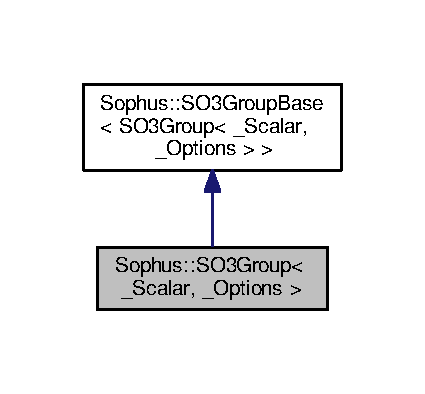
\includegraphics[width=204pt]{class_sophus_1_1_s_o3_group__inherit__graph}
\end{center}
\end{figure}


Collaboration diagram for Sophus\+:\+:S\+O3\+Group$<$ \+\_\+\+Scalar, \+\_\+\+Options $>$\+:
\nopagebreak
\begin{figure}[H]
\begin{center}
\leavevmode
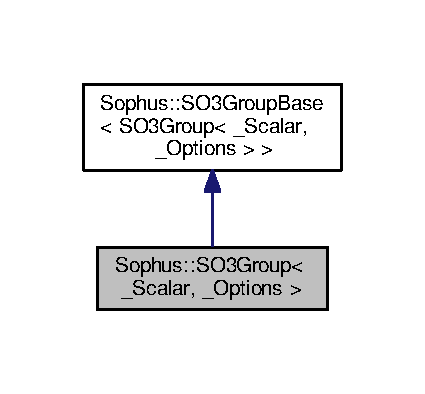
\includegraphics[width=204pt]{class_sophus_1_1_s_o3_group__coll__graph}
\end{center}
\end{figure}
\subsection*{Public Types}
\begin{DoxyCompactItemize}
\item 
typedef internal\+::traits$<$ \hyperlink{class_sophus_1_1_s_o3_group}{S\+O3\+Group}$<$ \+\_\+\+Scalar, \+\_\+\+Options $>$ $>$\+::\hyperlink{class_sophus_1_1_s_o3_group_a2b1432aa3eac9b174e41df7ce504cb06}{Scalar} \hyperlink{class_sophus_1_1_s_o3_group_a2b1432aa3eac9b174e41df7ce504cb06}{Scalar}\hypertarget{class_sophus_1_1_s_o3_group_a2b1432aa3eac9b174e41df7ce504cb06}{}\label{class_sophus_1_1_s_o3_group_a2b1432aa3eac9b174e41df7ce504cb06}

\begin{DoxyCompactList}\small\item\em scalar type \end{DoxyCompactList}\item 
typedef internal\+::traits$<$ \hyperlink{class_sophus_1_1_s_o3_group}{S\+O3\+Group}$<$ \+\_\+\+Scalar, \+\_\+\+Options $>$ $>$\+::Quaternion\+Type \& \hyperlink{class_sophus_1_1_s_o3_group_aaa65d0f058d31e972da558d6d909a2da}{Quaternion\+Reference}\hypertarget{class_sophus_1_1_s_o3_group_aaa65d0f058d31e972da558d6d909a2da}{}\label{class_sophus_1_1_s_o3_group_aaa65d0f058d31e972da558d6d909a2da}

\begin{DoxyCompactList}\small\item\em quaternion type \end{DoxyCompactList}\item 
typedef const internal\+::traits$<$ \hyperlink{class_sophus_1_1_s_o3_group}{S\+O3\+Group}$<$ \+\_\+\+Scalar, \+\_\+\+Options $>$ $>$\+::Quaternion\+Type \& {\bfseries Const\+Quaternion\+Reference}\hypertarget{class_sophus_1_1_s_o3_group_af8850e9ff5922a59ab5e6281fc2eaa89}{}\label{class_sophus_1_1_s_o3_group_af8850e9ff5922a59ab5e6281fc2eaa89}

\item 
typedef \hyperlink{class_sophus_1_1_s_o3_group_base_aa20fc57bf1b355a6616f5c4b785f1fc5}{Base\+::\+Transformation} \hyperlink{class_sophus_1_1_s_o3_group_a7fd4c61cae92c71a763d4f999c87fb9b}{Transformation}\hypertarget{class_sophus_1_1_s_o3_group_a7fd4c61cae92c71a763d4f999c87fb9b}{}\label{class_sophus_1_1_s_o3_group_a7fd4c61cae92c71a763d4f999c87fb9b}

\begin{DoxyCompactList}\small\item\em group transfomation type \end{DoxyCompactList}\item 
typedef \hyperlink{class_sophus_1_1_s_o3_group_base_a1cfbc3b3a28e1f70b3e1845716db0a1b}{Base\+::\+Point} \hyperlink{class_sophus_1_1_s_o3_group_aa56828c78f215b8c048304ae99d165c6}{Point}\hypertarget{class_sophus_1_1_s_o3_group_aa56828c78f215b8c048304ae99d165c6}{}\label{class_sophus_1_1_s_o3_group_aa56828c78f215b8c048304ae99d165c6}

\begin{DoxyCompactList}\small\item\em point type \end{DoxyCompactList}\item 
typedef \hyperlink{class_sophus_1_1_s_o3_group_base_a11150229b6a471ae96cde974ece5ec7c}{Base\+::\+Tangent} \hyperlink{class_sophus_1_1_s_o3_group_a313725e178a9d13c3cd38a78114a8e46}{Tangent}\hypertarget{class_sophus_1_1_s_o3_group_a313725e178a9d13c3cd38a78114a8e46}{}\label{class_sophus_1_1_s_o3_group_a313725e178a9d13c3cd38a78114a8e46}

\begin{DoxyCompactList}\small\item\em tangent vector type \end{DoxyCompactList}\item 
typedef \hyperlink{class_sophus_1_1_s_o3_group_base_a51c46f75563c21fbd223b4a444923306}{Base\+::\+Adjoint} \hyperlink{class_sophus_1_1_s_o3_group_aff34b2da7824cf564f4c6486eff961b4}{Adjoint}\hypertarget{class_sophus_1_1_s_o3_group_aff34b2da7824cf564f4c6486eff961b4}{}\label{class_sophus_1_1_s_o3_group_aff34b2da7824cf564f4c6486eff961b4}

\begin{DoxyCompactList}\small\item\em adjoint transformation type \end{DoxyCompactList}\end{DoxyCompactItemize}
\subsection*{Public Member Functions}
\begin{DoxyCompactItemize}
\item 
E\+I\+G\+E\+N\+\_\+\+M\+A\+K\+E\+\_\+\+A\+L\+I\+G\+N\+E\+D\+\_\+\+O\+P\+E\+R\+A\+T\+O\+R\+\_\+\+N\+EW \hyperlink{class_sophus_1_1_s_o3_group_a38ce610774b5a87bdb09260d0e8ee22b}{S\+O3\+Group} ()
\begin{DoxyCompactList}\small\item\em Default constructor. \end{DoxyCompactList}\item 
{\footnotesize template$<$typename Other\+Derived $>$ }\\\hyperlink{class_sophus_1_1_s_o3_group_a055e14e8c9ee93718c1570a7ef62447c}{S\+O3\+Group} (const \hyperlink{class_sophus_1_1_s_o3_group_base}{S\+O3\+Group\+Base}$<$ Other\+Derived $>$ \&other)\hypertarget{class_sophus_1_1_s_o3_group_a055e14e8c9ee93718c1570a7ef62447c}{}\label{class_sophus_1_1_s_o3_group_a055e14e8c9ee93718c1570a7ef62447c}

\begin{DoxyCompactList}\small\item\em Copy constructor. \end{DoxyCompactList}\item 
\hyperlink{class_sophus_1_1_s_o3_group_aca43c3b5f6a9f2376119c9d5e1b16f7f}{S\+O3\+Group} (const \hyperlink{class_sophus_1_1_s_o3_group_a7fd4c61cae92c71a763d4f999c87fb9b}{Transformation} \&R)
\begin{DoxyCompactList}\small\item\em Constructor from rotation matrix. \end{DoxyCompactList}\item 
\hyperlink{class_sophus_1_1_s_o3_group_a89369d9052724158090dfbaa96d803dd}{S\+O3\+Group} (const Quaternion$<$ \hyperlink{class_sophus_1_1_s_o3_group_a2b1432aa3eac9b174e41df7ce504cb06}{Scalar} $>$ \&quat)
\begin{DoxyCompactList}\small\item\em Constructor from quaternion. \end{DoxyCompactList}\item 
\hyperlink{class_sophus_1_1_s_o3_group_affa7204a5a51284edc7125eea9659014}{S\+O3\+Group} (\hyperlink{class_sophus_1_1_s_o3_group_a2b1432aa3eac9b174e41df7ce504cb06}{Scalar} alpha1, \hyperlink{class_sophus_1_1_s_o3_group_a2b1432aa3eac9b174e41df7ce504cb06}{Scalar} alpha2, \hyperlink{class_sophus_1_1_s_o3_group_a2b1432aa3eac9b174e41df7ce504cb06}{Scalar} alpha3)
\begin{DoxyCompactList}\small\item\em Constructor from Euler angles. \end{DoxyCompactList}\item 
E\+I\+G\+E\+N\+\_\+\+S\+T\+R\+O\+N\+G\+\_\+\+I\+N\+L\+I\+NE Const\+Quaternion\+Reference \hyperlink{class_sophus_1_1_s_o3_group_aa29eb341fa1c3a4b4addfe22e14e80a0}{unit\+\_\+quaternion} () const 
\begin{DoxyCompactList}\small\item\em Accessor of unit quaternion. \end{DoxyCompactList}\end{DoxyCompactItemize}
\subsection*{Static Public Attributes}
\begin{DoxyCompactItemize}
\item 
static const int \hyperlink{class_sophus_1_1_s_o3_group_a8a74ea9c68a0ffeca78fac87b1938a87}{DoF} = Base\+::\+DoF\hypertarget{class_sophus_1_1_s_o3_group_a8a74ea9c68a0ffeca78fac87b1938a87}{}\label{class_sophus_1_1_s_o3_group_a8a74ea9c68a0ffeca78fac87b1938a87}

\begin{DoxyCompactList}\small\item\em degree of freedom of group \end{DoxyCompactList}\item 
static const int \hyperlink{class_sophus_1_1_s_o3_group_a6406674167b756a348ac5bc61f58dc5d}{num\+\_\+parameters} = Base\+::num\+\_\+parameters\hypertarget{class_sophus_1_1_s_o3_group_a6406674167b756a348ac5bc61f58dc5d}{}\label{class_sophus_1_1_s_o3_group_a6406674167b756a348ac5bc61f58dc5d}

\begin{DoxyCompactList}\small\item\em number of internal parameters used \end{DoxyCompactList}\item 
static const int \hyperlink{class_sophus_1_1_s_o3_group_a8807fcc497570011e3b0bb419f17b84e}{N} = Base\+::N\hypertarget{class_sophus_1_1_s_o3_group_a8807fcc497570011e3b0bb419f17b84e}{}\label{class_sophus_1_1_s_o3_group_a8807fcc497570011e3b0bb419f17b84e}

\begin{DoxyCompactList}\small\item\em group transformations are NxN matrices \end{DoxyCompactList}\end{DoxyCompactItemize}
\subsection*{Protected Member Functions}
\begin{DoxyCompactItemize}
\item 
E\+I\+G\+E\+N\+\_\+\+S\+T\+R\+O\+N\+G\+\_\+\+I\+N\+L\+I\+NE \hyperlink{class_sophus_1_1_s_o3_group_aaa65d0f058d31e972da558d6d909a2da}{Quaternion\+Reference} {\bfseries unit\+\_\+quaternion\+\_\+nonconst} ()\hypertarget{class_sophus_1_1_s_o3_group_aacb9eb33c9157d0c77dfea2d35112b91}{}\label{class_sophus_1_1_s_o3_group_aacb9eb33c9157d0c77dfea2d35112b91}

\end{DoxyCompactItemize}
\subsection*{Protected Attributes}
\begin{DoxyCompactItemize}
\item 
Quaternion$<$ \hyperlink{class_sophus_1_1_s_o3_group_a2b1432aa3eac9b174e41df7ce504cb06}{Scalar} $>$ {\bfseries unit\+\_\+quaternion\+\_\+}\hypertarget{class_sophus_1_1_s_o3_group_ac5c0b33c11c656c72e9b631482c69327}{}\label{class_sophus_1_1_s_o3_group_ac5c0b33c11c656c72e9b631482c69327}

\end{DoxyCompactItemize}
\subsection*{Friends}
\begin{DoxyCompactItemize}
\item 
class {\bfseries S\+O3\+Group\+Base$<$ S\+O3\+Group$<$ \+\_\+\+Scalar, \+\_\+\+Options $>$ $>$}\hypertarget{class_sophus_1_1_s_o3_group_ab7750315d441a8277148bc479ef978d2}{}\label{class_sophus_1_1_s_o3_group_ab7750315d441a8277148bc479ef978d2}

\end{DoxyCompactItemize}
\subsection*{Additional Inherited Members}


\subsection{Detailed Description}
\subsubsection*{template$<$typename \+\_\+\+Scalar, int \+\_\+\+Options$>$\\*
class Sophus\+::\+S\+O3\+Group$<$ \+\_\+\+Scalar, \+\_\+\+Options $>$}

S\+O3 default type -\/ Constructors and default storage for S\+O3 Type. 

Definition at line 34 of file so3.\+hpp.



\subsection{Constructor \& Destructor Documentation}
\index{Sophus\+::\+S\+O3\+Group@{Sophus\+::\+S\+O3\+Group}!S\+O3\+Group@{S\+O3\+Group}}
\index{S\+O3\+Group@{S\+O3\+Group}!Sophus\+::\+S\+O3\+Group@{Sophus\+::\+S\+O3\+Group}}
\subsubsection[{\texorpdfstring{S\+O3\+Group()}{SO3Group()}}]{\setlength{\rightskip}{0pt plus 5cm}template$<$typename \+\_\+\+Scalar, int \+\_\+\+Options$>$ E\+I\+G\+E\+N\+\_\+\+M\+A\+K\+E\+\_\+\+A\+L\+I\+G\+N\+E\+D\+\_\+\+O\+P\+E\+R\+A\+T\+O\+R\+\_\+\+N\+EW {\bf Sophus\+::\+S\+O3\+Group}$<$ \+\_\+\+Scalar, \+\_\+\+Options $>$\+::{\bf S\+O3\+Group} (
\begin{DoxyParamCaption}
{}
\end{DoxyParamCaption}
)\hspace{0.3cm}{\ttfamily [inline]}}\hypertarget{class_sophus_1_1_s_o3_group_a38ce610774b5a87bdb09260d0e8ee22b}{}\label{class_sophus_1_1_s_o3_group_a38ce610774b5a87bdb09260d0e8ee22b}


Default constructor. 

Initialize Quaternion to identity rotation. 

Definition at line 603 of file so3.\+hpp.

\index{Sophus\+::\+S\+O3\+Group@{Sophus\+::\+S\+O3\+Group}!S\+O3\+Group@{S\+O3\+Group}}
\index{S\+O3\+Group@{S\+O3\+Group}!Sophus\+::\+S\+O3\+Group@{Sophus\+::\+S\+O3\+Group}}
\subsubsection[{\texorpdfstring{S\+O3\+Group(const Transformation \&\+R)}{SO3Group(const Transformation &R)}}]{\setlength{\rightskip}{0pt plus 5cm}template$<$typename \+\_\+\+Scalar, int \+\_\+\+Options$>$ {\bf Sophus\+::\+S\+O3\+Group}$<$ \+\_\+\+Scalar, \+\_\+\+Options $>$\+::{\bf S\+O3\+Group} (
\begin{DoxyParamCaption}
\item[{const {\bf Transformation} \&}]{R}
\end{DoxyParamCaption}
)\hspace{0.3cm}{\ttfamily [inline]}}\hypertarget{class_sophus_1_1_s_o3_group_aca43c3b5f6a9f2376119c9d5e1b16f7f}{}\label{class_sophus_1_1_s_o3_group_aca43c3b5f6a9f2376119c9d5e1b16f7f}


Constructor from rotation matrix. 

\begin{DoxyPrecond}{Precondition}
rotation matrix need to be orthogonal with determinant of 1 
\end{DoxyPrecond}


Definition at line 621 of file so3.\+hpp.

\index{Sophus\+::\+S\+O3\+Group@{Sophus\+::\+S\+O3\+Group}!S\+O3\+Group@{S\+O3\+Group}}
\index{S\+O3\+Group@{S\+O3\+Group}!Sophus\+::\+S\+O3\+Group@{Sophus\+::\+S\+O3\+Group}}
\subsubsection[{\texorpdfstring{S\+O3\+Group(const Quaternion$<$ Scalar $>$ \&quat)}{SO3Group(const Quaternion< Scalar > &quat)}}]{\setlength{\rightskip}{0pt plus 5cm}template$<$typename \+\_\+\+Scalar, int \+\_\+\+Options$>$ {\bf Sophus\+::\+S\+O3\+Group}$<$ \+\_\+\+Scalar, \+\_\+\+Options $>$\+::{\bf S\+O3\+Group} (
\begin{DoxyParamCaption}
\item[{const Quaternion$<$ {\bf Scalar} $>$ \&}]{quat}
\end{DoxyParamCaption}
)\hspace{0.3cm}{\ttfamily [inline]}, {\ttfamily [explicit]}}\hypertarget{class_sophus_1_1_s_o3_group_a89369d9052724158090dfbaa96d803dd}{}\label{class_sophus_1_1_s_o3_group_a89369d9052724158090dfbaa96d803dd}


Constructor from quaternion. 

\begin{DoxyPrecond}{Precondition}
quaternion must not be zero 
\end{DoxyPrecond}


Definition at line 631 of file so3.\+hpp.

\index{Sophus\+::\+S\+O3\+Group@{Sophus\+::\+S\+O3\+Group}!S\+O3\+Group@{S\+O3\+Group}}
\index{S\+O3\+Group@{S\+O3\+Group}!Sophus\+::\+S\+O3\+Group@{Sophus\+::\+S\+O3\+Group}}
\subsubsection[{\texorpdfstring{S\+O3\+Group(\+Scalar alpha1, Scalar alpha2, Scalar alpha3)}{SO3Group(Scalar alpha1, Scalar alpha2, Scalar alpha3)}}]{\setlength{\rightskip}{0pt plus 5cm}template$<$typename \+\_\+\+Scalar, int \+\_\+\+Options$>$ {\bf Sophus\+::\+S\+O3\+Group}$<$ \+\_\+\+Scalar, \+\_\+\+Options $>$\+::{\bf S\+O3\+Group} (
\begin{DoxyParamCaption}
\item[{{\bf Scalar}}]{alpha1, }
\item[{{\bf Scalar}}]{alpha2, }
\item[{{\bf Scalar}}]{alpha3}
\end{DoxyParamCaption}
)\hspace{0.3cm}{\ttfamily [inline]}}\hypertarget{class_sophus_1_1_s_o3_group_affa7204a5a51284edc7125eea9659014}{}\label{class_sophus_1_1_s_o3_group_affa7204a5a51284edc7125eea9659014}


Constructor from Euler angles. 


\begin{DoxyParams}{Parameters}
{\em alpha1} & rotation around x-\/axis \\
\hline
{\em alpha2} & rotation around y-\/axis \\
\hline
{\em alpha3} & rotation around z-\/axis\\
\hline
\end{DoxyParams}
Since rotations in 3D do not commute, the order of the individual rotations matter. Here, the following convention is used. We calculate a S\+O3 member corresponding to the rotation matrix $ R $ such that $ R=\exp\left(\begin{array}{c}\alpha_1\\ 0\\ 0\end{array}\right) \cdot \exp\left(\begin{array}{c}0\\ \alpha_2\\ 0\end{array}\right) \cdot \exp\left(\begin{array}{c}0\\ 0\\ \alpha_3\end{array}\right)$. 

Definition at line 650 of file so3.\+hpp.



\subsection{Member Function Documentation}
\index{Sophus\+::\+S\+O3\+Group@{Sophus\+::\+S\+O3\+Group}!unit\+\_\+quaternion@{unit\+\_\+quaternion}}
\index{unit\+\_\+quaternion@{unit\+\_\+quaternion}!Sophus\+::\+S\+O3\+Group@{Sophus\+::\+S\+O3\+Group}}
\subsubsection[{\texorpdfstring{unit\+\_\+quaternion() const }{unit_quaternion() const }}]{\setlength{\rightskip}{0pt plus 5cm}template$<$typename \+\_\+\+Scalar, int \+\_\+\+Options$>$ E\+I\+G\+E\+N\+\_\+\+S\+T\+R\+O\+N\+G\+\_\+\+I\+N\+L\+I\+NE Const\+Quaternion\+Reference {\bf Sophus\+::\+S\+O3\+Group}$<$ \+\_\+\+Scalar, \+\_\+\+Options $>$\+::unit\+\_\+quaternion (
\begin{DoxyParamCaption}
{}
\end{DoxyParamCaption}
) const\hspace{0.3cm}{\ttfamily [inline]}}\hypertarget{class_sophus_1_1_s_o3_group_aa29eb341fa1c3a4b4addfe22e14e80a0}{}\label{class_sophus_1_1_s_o3_group_aa29eb341fa1c3a4b4addfe22e14e80a0}


Accessor of unit quaternion. 

No direct write access is given to ensure the quaternion stays normalized. 

Definition at line 665 of file so3.\+hpp.



The documentation for this class was generated from the following file\+:\begin{DoxyCompactItemize}
\item 
include/\+Sophus/sophus/so3.\+hpp\end{DoxyCompactItemize}

\hypertarget{class_sophus_1_1_s_o3_group_base}{}\section{Sophus\+:\+:S\+O3\+Group\+Base$<$ Derived $>$ Class Template Reference}
\label{class_sophus_1_1_s_o3_group_base}\index{Sophus\+::\+S\+O3\+Group\+Base$<$ Derived $>$@{Sophus\+::\+S\+O3\+Group\+Base$<$ Derived $>$}}


S\+O3 base type -\/ implements S\+O3 class but is storage agnostic.  




{\ttfamily \#include $<$so3.\+hpp$>$}



Inheritance diagram for Sophus\+:\+:S\+O3\+Group\+Base$<$ Derived $>$\+:
\nopagebreak
\begin{figure}[H]
\begin{center}
\leavevmode
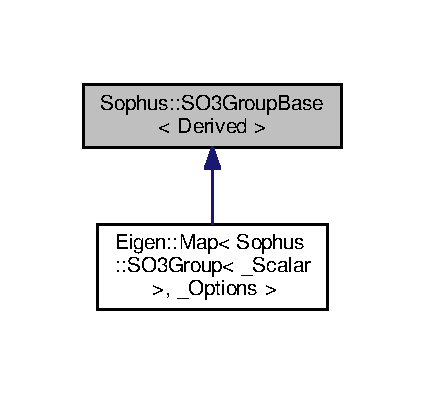
\includegraphics[width=204pt]{class_sophus_1_1_s_o3_group_base__inherit__graph}
\end{center}
\end{figure}
\subsection*{Public Types}
\begin{DoxyCompactItemize}
\item 
typedef internal\+::traits$<$ Derived $>$\+::\hyperlink{class_sophus_1_1_s_o3_group_base_a31bf31815c195b7150da8a8e8c6f0189}{Scalar} \hyperlink{class_sophus_1_1_s_o3_group_base_a31bf31815c195b7150da8a8e8c6f0189}{Scalar}\hypertarget{class_sophus_1_1_s_o3_group_base_a31bf31815c195b7150da8a8e8c6f0189}{}\label{class_sophus_1_1_s_o3_group_base_a31bf31815c195b7150da8a8e8c6f0189}

\begin{DoxyCompactList}\small\item\em scalar type \end{DoxyCompactList}\item 
typedef internal\+::traits$<$ Derived $>$\+::Quaternion\+Type \& \hyperlink{class_sophus_1_1_s_o3_group_base_af58920cc70e59d58dcf427a22ebacaeb}{Quaternion\+Reference}\hypertarget{class_sophus_1_1_s_o3_group_base_af58920cc70e59d58dcf427a22ebacaeb}{}\label{class_sophus_1_1_s_o3_group_base_af58920cc70e59d58dcf427a22ebacaeb}

\begin{DoxyCompactList}\small\item\em quaternion reference type \end{DoxyCompactList}\item 
typedef const internal\+::traits$<$ Derived $>$\+::Quaternion\+Type \& \hyperlink{class_sophus_1_1_s_o3_group_base_a8a5a23aee10f2850a5894b7c1f5e6654}{Const\+Quaternion\+Reference}\hypertarget{class_sophus_1_1_s_o3_group_base_a8a5a23aee10f2850a5894b7c1f5e6654}{}\label{class_sophus_1_1_s_o3_group_base_a8a5a23aee10f2850a5894b7c1f5e6654}

\begin{DoxyCompactList}\small\item\em quaternion const reference type \end{DoxyCompactList}\item 
typedef Matrix$<$ \hyperlink{class_sophus_1_1_s_o3_group_base_a31bf31815c195b7150da8a8e8c6f0189}{Scalar}, \hyperlink{class_sophus_1_1_s_o3_group_base_ad7937061e3b4eab530142d5e1a1921c2}{N}, \hyperlink{class_sophus_1_1_s_o3_group_base_ad7937061e3b4eab530142d5e1a1921c2}{N} $>$ \hyperlink{class_sophus_1_1_s_o3_group_base_aa20fc57bf1b355a6616f5c4b785f1fc5}{Transformation}\hypertarget{class_sophus_1_1_s_o3_group_base_aa20fc57bf1b355a6616f5c4b785f1fc5}{}\label{class_sophus_1_1_s_o3_group_base_aa20fc57bf1b355a6616f5c4b785f1fc5}

\begin{DoxyCompactList}\small\item\em group transfomation type \end{DoxyCompactList}\item 
typedef Matrix$<$ \hyperlink{class_sophus_1_1_s_o3_group_base_a31bf31815c195b7150da8a8e8c6f0189}{Scalar}, 3, 1 $>$ \hyperlink{class_sophus_1_1_s_o3_group_base_a1cfbc3b3a28e1f70b3e1845716db0a1b}{Point}\hypertarget{class_sophus_1_1_s_o3_group_base_a1cfbc3b3a28e1f70b3e1845716db0a1b}{}\label{class_sophus_1_1_s_o3_group_base_a1cfbc3b3a28e1f70b3e1845716db0a1b}

\begin{DoxyCompactList}\small\item\em point type \end{DoxyCompactList}\item 
typedef Matrix$<$ \hyperlink{class_sophus_1_1_s_o3_group_base_a31bf31815c195b7150da8a8e8c6f0189}{Scalar}, \hyperlink{class_sophus_1_1_s_o3_group_base_ad12ec6c47a2206217f337ea90884b4c1}{DoF}, 1 $>$ \hyperlink{class_sophus_1_1_s_o3_group_base_a11150229b6a471ae96cde974ece5ec7c}{Tangent}\hypertarget{class_sophus_1_1_s_o3_group_base_a11150229b6a471ae96cde974ece5ec7c}{}\label{class_sophus_1_1_s_o3_group_base_a11150229b6a471ae96cde974ece5ec7c}

\begin{DoxyCompactList}\small\item\em tangent vector type \end{DoxyCompactList}\item 
typedef Matrix$<$ \hyperlink{class_sophus_1_1_s_o3_group_base_a31bf31815c195b7150da8a8e8c6f0189}{Scalar}, \hyperlink{class_sophus_1_1_s_o3_group_base_ad12ec6c47a2206217f337ea90884b4c1}{DoF}, \hyperlink{class_sophus_1_1_s_o3_group_base_ad12ec6c47a2206217f337ea90884b4c1}{DoF} $>$ \hyperlink{class_sophus_1_1_s_o3_group_base_a51c46f75563c21fbd223b4a444923306}{Adjoint}\hypertarget{class_sophus_1_1_s_o3_group_base_a51c46f75563c21fbd223b4a444923306}{}\label{class_sophus_1_1_s_o3_group_base_a51c46f75563c21fbd223b4a444923306}

\begin{DoxyCompactList}\small\item\em adjoint transformation type \end{DoxyCompactList}\end{DoxyCompactItemize}
\subsection*{Public Member Functions}
\begin{DoxyCompactItemize}
\item 
const \hyperlink{class_sophus_1_1_s_o3_group_base_a51c46f75563c21fbd223b4a444923306}{Adjoint} \hyperlink{class_sophus_1_1_s_o3_group_base_a938f2e50857b65bac1babcee269b9d86}{Adj} () const 
\begin{DoxyCompactList}\small\item\em Adjoint transformation. \end{DoxyCompactList}\item 
{\footnotesize template$<$typename New\+Scalar\+Type $>$ }\\\hyperlink{class_sophus_1_1_s_o3_group}{S\+O3\+Group}$<$ New\+Scalar\+Type $>$ \hyperlink{class_sophus_1_1_s_o3_group_base_a2be02c8110c6d160603be88a88336d52}{cast} () const 
\item 
\hyperlink{class_sophus_1_1_s_o3_group_base_a31bf31815c195b7150da8a8e8c6f0189}{Scalar} $\ast$ \hyperlink{class_sophus_1_1_s_o3_group_base_a2fbf1faa2799543e1f42df71bafe3b80}{data} ()
\item 
const \hyperlink{class_sophus_1_1_s_o3_group_base_a31bf31815c195b7150da8a8e8c6f0189}{Scalar} $\ast$ \hyperlink{class_sophus_1_1_s_o3_group_base_afe2f2724f7df77160f63161c20a245f1}{data} () const 
\item 
void \hyperlink{class_sophus_1_1_s_o3_group_base_aa0ed45f31d37bb97c60c839f680bed44}{fast\+Multiply} (const \hyperlink{class_sophus_1_1_s_o3_group}{S\+O3\+Group}$<$ \hyperlink{class_sophus_1_1_s_o3_group_base_a31bf31815c195b7150da8a8e8c6f0189}{Scalar} $>$ \&other)
\begin{DoxyCompactList}\small\item\em Fast group multiplication. \end{DoxyCompactList}\item 
const \hyperlink{class_sophus_1_1_s_o3_group}{S\+O3\+Group}$<$ \hyperlink{class_sophus_1_1_s_o3_group_base_a31bf31815c195b7150da8a8e8c6f0189}{Scalar} $>$ \hyperlink{class_sophus_1_1_s_o3_group_base_a8b22195a0b01980b2656ed838c39cee9}{inverse} () const 
\item 
const \hyperlink{class_sophus_1_1_s_o3_group_base_a11150229b6a471ae96cde974ece5ec7c}{Tangent} \hyperlink{class_sophus_1_1_s_o3_group_base_ae4196d42fc37f6dddb987bfb726575a5}{log} () const 
\begin{DoxyCompactList}\small\item\em Logarithmic map. \end{DoxyCompactList}\item 
void \hyperlink{class_sophus_1_1_s_o3_group_base_a10c6863560f5bac15d13d1916c3cda95}{normalize} ()
\begin{DoxyCompactList}\small\item\em Normalize quaternion. \end{DoxyCompactList}\item 
const \hyperlink{class_sophus_1_1_s_o3_group_base_aa20fc57bf1b355a6616f5c4b785f1fc5}{Transformation} \hyperlink{class_sophus_1_1_s_o3_group_base_adc29d15481f673ccfcae77b065ea38be}{matrix} () const 
\item 
{\footnotesize template$<$typename Other\+Derived $>$ }\\\hyperlink{class_sophus_1_1_s_o3_group_base}{S\+O3\+Group\+Base}$<$ Derived $>$ \& \hyperlink{class_sophus_1_1_s_o3_group_base_a041893de9d3e7ddb5c0bd12add57319b}{operator=} (const \hyperlink{class_sophus_1_1_s_o3_group_base}{S\+O3\+Group\+Base}$<$ Other\+Derived $>$ \&other)\hypertarget{class_sophus_1_1_s_o3_group_base_a041893de9d3e7ddb5c0bd12add57319b}{}\label{class_sophus_1_1_s_o3_group_base_a041893de9d3e7ddb5c0bd12add57319b}

\begin{DoxyCompactList}\small\item\em Assignment operator. \end{DoxyCompactList}\item 
const \hyperlink{class_sophus_1_1_s_o3_group}{S\+O3\+Group}$<$ \hyperlink{class_sophus_1_1_s_o3_group_base_a31bf31815c195b7150da8a8e8c6f0189}{Scalar} $>$ \hyperlink{class_sophus_1_1_s_o3_group_base_af3924b64a1a6c45946f80f4e88f04a6d}{operator$\ast$} (const \hyperlink{class_sophus_1_1_s_o3_group}{S\+O3\+Group}$<$ \hyperlink{class_sophus_1_1_s_o3_group_base_a31bf31815c195b7150da8a8e8c6f0189}{Scalar} $>$ \&other) const 
\begin{DoxyCompactList}\small\item\em Group multiplication. \end{DoxyCompactList}\item 
const \hyperlink{class_sophus_1_1_s_o3_group_base_a1cfbc3b3a28e1f70b3e1845716db0a1b}{Point} \hyperlink{class_sophus_1_1_s_o3_group_base_ad627562967215f7bd4ba593925b871bd}{operator$\ast$} (const \hyperlink{class_sophus_1_1_s_o3_group_base_a1cfbc3b3a28e1f70b3e1845716db0a1b}{Point} \&p) const 
\begin{DoxyCompactList}\small\item\em Group action on $ \mathbf{R}^3 $. \end{DoxyCompactList}\item 
void \hyperlink{class_sophus_1_1_s_o3_group_base_aeb9fd0d8089a51a9a0a0ad08eba1a8a0}{operator$\ast$=} (const \hyperlink{class_sophus_1_1_s_o3_group}{S\+O3\+Group}$<$ \hyperlink{class_sophus_1_1_s_o3_group_base_a31bf31815c195b7150da8a8e8c6f0189}{Scalar} $>$ \&other)
\begin{DoxyCompactList}\small\item\em In-\/place group multiplication. \end{DoxyCompactList}\item 
void \hyperlink{class_sophus_1_1_s_o3_group_base_aacf1cdcbeb6ebff5ab5f86ad015c16f9}{set\+Quaternion} (const Quaternion$<$ \hyperlink{class_sophus_1_1_s_o3_group_base_a31bf31815c195b7150da8a8e8c6f0189}{Scalar} $>$ \&quaternion)
\begin{DoxyCompactList}\small\item\em Setter of internal unit quaternion representation. \end{DoxyCompactList}\item 
E\+I\+G\+E\+N\+\_\+\+S\+T\+R\+O\+N\+G\+\_\+\+I\+N\+L\+I\+NE \hyperlink{class_sophus_1_1_s_o3_group_base_a8a5a23aee10f2850a5894b7c1f5e6654}{Const\+Quaternion\+Reference} \hyperlink{class_sophus_1_1_s_o3_group_base_ab36e91f1f0ffce4be8a5f26902216832}{unit\+\_\+quaternion} () const 
\begin{DoxyCompactList}\small\item\em Accessor of unit quaternion. \end{DoxyCompactList}\end{DoxyCompactItemize}
\subsection*{Static Public Member Functions}
\begin{DoxyCompactItemize}
\item 
static const \hyperlink{class_sophus_1_1_s_o3_group_base_a51c46f75563c21fbd223b4a444923306}{Adjoint} \hyperlink{class_sophus_1_1_s_o3_group_base_a9b89eaf13ca40eb929ce3bc02b71f592}{d\+\_\+lie\+Bracketab\+\_\+by\+\_\+d\+\_\+a} (const \hyperlink{class_sophus_1_1_s_o3_group_base_a11150229b6a471ae96cde974ece5ec7c}{Tangent} \&b)
\item 
static const \hyperlink{class_sophus_1_1_s_o3_group}{S\+O3\+Group}$<$ \hyperlink{class_sophus_1_1_s_o3_group_base_a31bf31815c195b7150da8a8e8c6f0189}{Scalar} $>$ \hyperlink{class_sophus_1_1_s_o3_group_base_a7d224bfb20704608dc41e5a5f16ba9a4}{exp} (const \hyperlink{class_sophus_1_1_s_o3_group_base_a11150229b6a471ae96cde974ece5ec7c}{Tangent} \&omega)
\begin{DoxyCompactList}\small\item\em Group exponential. \end{DoxyCompactList}\item 
static const \hyperlink{class_sophus_1_1_s_o3_group}{S\+O3\+Group}$<$ \hyperlink{class_sophus_1_1_s_o3_group_base_a31bf31815c195b7150da8a8e8c6f0189}{Scalar} $>$ \hyperlink{class_sophus_1_1_s_o3_group_base_a79e8ae77c3461891a8eb2e2b4103c87c}{exp\+And\+Theta} (const \hyperlink{class_sophus_1_1_s_o3_group_base_a11150229b6a471ae96cde974ece5ec7c}{Tangent} \&omega, \hyperlink{class_sophus_1_1_s_o3_group_base_a31bf31815c195b7150da8a8e8c6f0189}{Scalar} $\ast$theta)
\begin{DoxyCompactList}\small\item\em Group exponential and theta. \end{DoxyCompactList}\item 
static const \hyperlink{class_sophus_1_1_s_o3_group_base_aa20fc57bf1b355a6616f5c4b785f1fc5}{Transformation} \hyperlink{class_sophus_1_1_s_o3_group_base_a06c9fd7d013a557fdc92e7983b1f75ac}{generator} (int i)
\begin{DoxyCompactList}\small\item\em Generators. \end{DoxyCompactList}\item 
static const \hyperlink{class_sophus_1_1_s_o3_group_base_aa20fc57bf1b355a6616f5c4b785f1fc5}{Transformation} \hyperlink{class_sophus_1_1_s_o3_group_base_a330c86d19073bb2d142d88078d92a513}{hat} (const \hyperlink{class_sophus_1_1_s_o3_group_base_a11150229b6a471ae96cde974ece5ec7c}{Tangent} \&omega)
\begin{DoxyCompactList}\small\item\em hat-\/operator \end{DoxyCompactList}\item 
static const \hyperlink{class_sophus_1_1_s_o3_group_base_a11150229b6a471ae96cde974ece5ec7c}{Tangent} \hyperlink{class_sophus_1_1_s_o3_group_base_a42bf7d9f6ddb6c3e71070df9f4f64f82}{lie\+Bracket} (const \hyperlink{class_sophus_1_1_s_o3_group_base_a11150229b6a471ae96cde974ece5ec7c}{Tangent} \&omega1, const \hyperlink{class_sophus_1_1_s_o3_group_base_a11150229b6a471ae96cde974ece5ec7c}{Tangent} \&omega2)
\begin{DoxyCompactList}\small\item\em Lie bracket. \end{DoxyCompactList}\item 
static const \hyperlink{class_sophus_1_1_s_o3_group_base_a11150229b6a471ae96cde974ece5ec7c}{Tangent} \hyperlink{class_sophus_1_1_s_o3_group_base_ad88c991746d629cefa056a44ed91f902}{log} (const \hyperlink{class_sophus_1_1_s_o3_group}{S\+O3\+Group}$<$ \hyperlink{class_sophus_1_1_s_o3_group_base_a31bf31815c195b7150da8a8e8c6f0189}{Scalar} $>$ \&other)
\begin{DoxyCompactList}\small\item\em Logarithmic map. \end{DoxyCompactList}\item 
static const \hyperlink{class_sophus_1_1_s_o3_group_base_a11150229b6a471ae96cde974ece5ec7c}{Tangent} \hyperlink{class_sophus_1_1_s_o3_group_base_a4d568828a5967d08364aa6a3439ccb79}{log\+And\+Theta} (const \hyperlink{class_sophus_1_1_s_o3_group}{S\+O3\+Group}$<$ \hyperlink{class_sophus_1_1_s_o3_group_base_a31bf31815c195b7150da8a8e8c6f0189}{Scalar} $>$ \&other, \hyperlink{class_sophus_1_1_s_o3_group_base_a31bf31815c195b7150da8a8e8c6f0189}{Scalar} $\ast$theta)
\begin{DoxyCompactList}\small\item\em Logarithmic map and theta. \end{DoxyCompactList}\item 
static const \hyperlink{class_sophus_1_1_s_o3_group_base_a11150229b6a471ae96cde974ece5ec7c}{Tangent} \hyperlink{class_sophus_1_1_s_o3_group_base_aee724215d80386327f000bb0c5cc376c}{vee} (const \hyperlink{class_sophus_1_1_s_o3_group_base_aa20fc57bf1b355a6616f5c4b785f1fc5}{Transformation} \&Omega)
\begin{DoxyCompactList}\small\item\em vee-\/operator \end{DoxyCompactList}\end{DoxyCompactItemize}
\subsection*{Static Public Attributes}
\begin{DoxyCompactItemize}
\item 
static const int \hyperlink{class_sophus_1_1_s_o3_group_base_ad12ec6c47a2206217f337ea90884b4c1}{DoF} = 3\hypertarget{class_sophus_1_1_s_o3_group_base_ad12ec6c47a2206217f337ea90884b4c1}{}\label{class_sophus_1_1_s_o3_group_base_ad12ec6c47a2206217f337ea90884b4c1}

\begin{DoxyCompactList}\small\item\em degree of freedom of group (three for rotation) \end{DoxyCompactList}\item 
static const int \hyperlink{class_sophus_1_1_s_o3_group_base_ae2da1635f11e6648cc869c458c6d4251}{num\+\_\+parameters} = 4\hypertarget{class_sophus_1_1_s_o3_group_base_ae2da1635f11e6648cc869c458c6d4251}{}\label{class_sophus_1_1_s_o3_group_base_ae2da1635f11e6648cc869c458c6d4251}

\begin{DoxyCompactList}\small\item\em number of internal parameters used (unit quaternion for rotation) \end{DoxyCompactList}\item 
static const int \hyperlink{class_sophus_1_1_s_o3_group_base_ad7937061e3b4eab530142d5e1a1921c2}{N} = 3\hypertarget{class_sophus_1_1_s_o3_group_base_ad7937061e3b4eab530142d5e1a1921c2}{}\label{class_sophus_1_1_s_o3_group_base_ad7937061e3b4eab530142d5e1a1921c2}

\begin{DoxyCompactList}\small\item\em group transformations are NxN matrices \end{DoxyCompactList}\end{DoxyCompactItemize}


\subsection{Detailed Description}
\subsubsection*{template$<$typename Derived$>$\\*
class Sophus\+::\+S\+O3\+Group\+Base$<$ Derived $>$}

S\+O3 base type -\/ implements S\+O3 class but is storage agnostic. 

\mbox{[}add more detailed description/tutorial\mbox{]} 

Definition at line 79 of file so3.\+hpp.



\subsection{Member Function Documentation}
\index{Sophus\+::\+S\+O3\+Group\+Base@{Sophus\+::\+S\+O3\+Group\+Base}!Adj@{Adj}}
\index{Adj@{Adj}!Sophus\+::\+S\+O3\+Group\+Base@{Sophus\+::\+S\+O3\+Group\+Base}}
\subsubsection[{\texorpdfstring{Adj() const }{Adj() const }}]{\setlength{\rightskip}{0pt plus 5cm}template$<$typename Derived$>$ const {\bf Adjoint} {\bf Sophus\+::\+S\+O3\+Group\+Base}$<$ Derived $>$\+::Adj (
\begin{DoxyParamCaption}
{}
\end{DoxyParamCaption}
) const\hspace{0.3cm}{\ttfamily [inline]}}\hypertarget{class_sophus_1_1_s_o3_group_base_a938f2e50857b65bac1babcee269b9d86}{}\label{class_sophus_1_1_s_o3_group_base_a938f2e50857b65bac1babcee269b9d86}


Adjoint transformation. 

This function return the adjoint transformation $ Ad $ of the group instance $ A $ such that for all $ x $ it holds that $ \widehat{Ad_A\cdot x} = A\widehat{x}A^{-1} $ with $\ \widehat{\cdot} $ being the \hyperlink{class_sophus_1_1_s_o3_group_base_a330c86d19073bb2d142d88078d92a513}{hat()}-\/\+Vector4\+Scalaror.

For S\+O3, it simply returns the rotation matrix corresponding to $ A $. 

Definition at line 118 of file so3.\+hpp.

\index{Sophus\+::\+S\+O3\+Group\+Base@{Sophus\+::\+S\+O3\+Group\+Base}!cast@{cast}}
\index{cast@{cast}!Sophus\+::\+S\+O3\+Group\+Base@{Sophus\+::\+S\+O3\+Group\+Base}}
\subsubsection[{\texorpdfstring{cast() const }{cast() const }}]{\setlength{\rightskip}{0pt plus 5cm}template$<$typename Derived$>$ template$<$typename New\+Scalar\+Type $>$ {\bf S\+O3\+Group}$<$New\+Scalar\+Type$>$ {\bf Sophus\+::\+S\+O3\+Group\+Base}$<$ Derived $>$\+::cast (
\begin{DoxyParamCaption}
{}
\end{DoxyParamCaption}
) const\hspace{0.3cm}{\ttfamily [inline]}}\hypertarget{class_sophus_1_1_s_o3_group_base_a2be02c8110c6d160603be88a88336d52}{}\label{class_sophus_1_1_s_o3_group_base_a2be02c8110c6d160603be88a88336d52}
\begin{DoxyReturn}{Returns}
copy of instance casted to New\+Scalar\+Type 
\end{DoxyReturn}


Definition at line 126 of file so3.\+hpp.

\index{Sophus\+::\+S\+O3\+Group\+Base@{Sophus\+::\+S\+O3\+Group\+Base}!d\+\_\+lie\+Bracketab\+\_\+by\+\_\+d\+\_\+a@{d\+\_\+lie\+Bracketab\+\_\+by\+\_\+d\+\_\+a}}
\index{d\+\_\+lie\+Bracketab\+\_\+by\+\_\+d\+\_\+a@{d\+\_\+lie\+Bracketab\+\_\+by\+\_\+d\+\_\+a}!Sophus\+::\+S\+O3\+Group\+Base@{Sophus\+::\+S\+O3\+Group\+Base}}
\subsubsection[{\texorpdfstring{d\+\_\+lie\+Bracketab\+\_\+by\+\_\+d\+\_\+a(const Tangent \&b)}{d_lieBracketab_by_d_a(const Tangent &b)}}]{\setlength{\rightskip}{0pt plus 5cm}template$<$typename Derived$>$ static const {\bf Adjoint} {\bf Sophus\+::\+S\+O3\+Group\+Base}$<$ Derived $>$\+::d\+\_\+lie\+Bracketab\+\_\+by\+\_\+d\+\_\+a (
\begin{DoxyParamCaption}
\item[{const {\bf Tangent} \&}]{b}
\end{DoxyParamCaption}
)\hspace{0.3cm}{\ttfamily [inline]}, {\ttfamily [static]}}\hypertarget{class_sophus_1_1_s_o3_group_base_a9b89eaf13ca40eb929ce3bc02b71f592}{}\label{class_sophus_1_1_s_o3_group_base_a9b89eaf13ca40eb929ce3bc02b71f592}

\begin{DoxyParams}{Parameters}
{\em b} & 3-\/vector representation of Lie algebra element \\
\hline
\end{DoxyParams}
\begin{DoxyReturn}{Returns}
derivative of Lie bracket
\end{DoxyReturn}
This function returns $ \frac{\partial}{\partial a} [a, b]_{so3} $ with $ [a, b]_{so3} $ being the \hyperlink{class_sophus_1_1_s_o3_group_base_a42bf7d9f6ddb6c3e71070df9f4f64f82}{lie\+Bracket()} of the Lie algebra so3.

\begin{DoxySeeAlso}{See also}
\hyperlink{class_sophus_1_1_s_o3_group_base_a42bf7d9f6ddb6c3e71070df9f4f64f82}{lie\+Bracket()} 
\end{DoxySeeAlso}


Definition at line 309 of file so3.\+hpp.

\index{Sophus\+::\+S\+O3\+Group\+Base@{Sophus\+::\+S\+O3\+Group\+Base}!data@{data}}
\index{data@{data}!Sophus\+::\+S\+O3\+Group\+Base@{Sophus\+::\+S\+O3\+Group\+Base}}
\subsubsection[{\texorpdfstring{data()}{data()}}]{\setlength{\rightskip}{0pt plus 5cm}template$<$typename Derived$>$ {\bf Scalar}$\ast$ {\bf Sophus\+::\+S\+O3\+Group\+Base}$<$ Derived $>$\+::data (
\begin{DoxyParamCaption}
{}
\end{DoxyParamCaption}
)\hspace{0.3cm}{\ttfamily [inline]}}\hypertarget{class_sophus_1_1_s_o3_group_base_a2fbf1faa2799543e1f42df71bafe3b80}{}\label{class_sophus_1_1_s_o3_group_base_a2fbf1faa2799543e1f42df71bafe3b80}
\begin{DoxyReturn}{Returns}
pointer to internal data
\end{DoxyReturn}
This provides unsafe read/write access to internal data. S\+O3 is represented by an Eigen\+::\+Quaternion (four parameters). When using direct write access, the user needs to take care of that the quaternion stays normalized.

Note\+: The first three Scalars represent the imaginary parts, while the forth Scalar represent the real part.

\begin{DoxySeeAlso}{See also}
\hyperlink{class_sophus_1_1_s_o3_group_base_a10c6863560f5bac15d13d1916c3cda95}{normalize()} 
\end{DoxySeeAlso}


Definition at line 143 of file so3.\+hpp.

\index{Sophus\+::\+S\+O3\+Group\+Base@{Sophus\+::\+S\+O3\+Group\+Base}!data@{data}}
\index{data@{data}!Sophus\+::\+S\+O3\+Group\+Base@{Sophus\+::\+S\+O3\+Group\+Base}}
\subsubsection[{\texorpdfstring{data() const }{data() const }}]{\setlength{\rightskip}{0pt plus 5cm}template$<$typename Derived$>$ const {\bf Scalar}$\ast$ {\bf Sophus\+::\+S\+O3\+Group\+Base}$<$ Derived $>$\+::data (
\begin{DoxyParamCaption}
{}
\end{DoxyParamCaption}
) const\hspace{0.3cm}{\ttfamily [inline]}}\hypertarget{class_sophus_1_1_s_o3_group_base_afe2f2724f7df77160f63161c20a245f1}{}\label{class_sophus_1_1_s_o3_group_base_afe2f2724f7df77160f63161c20a245f1}
\begin{DoxyReturn}{Returns}
const pointer to internal data
\end{DoxyReturn}
Const version of \hyperlink{class_sophus_1_1_s_o3_group_base_a2fbf1faa2799543e1f42df71bafe3b80}{data()}. 

Definition at line 152 of file so3.\+hpp.

\index{Sophus\+::\+S\+O3\+Group\+Base@{Sophus\+::\+S\+O3\+Group\+Base}!exp@{exp}}
\index{exp@{exp}!Sophus\+::\+S\+O3\+Group\+Base@{Sophus\+::\+S\+O3\+Group\+Base}}
\subsubsection[{\texorpdfstring{exp(const Tangent \&omega)}{exp(const Tangent &omega)}}]{\setlength{\rightskip}{0pt plus 5cm}template$<$typename Derived$>$ static const {\bf S\+O3\+Group}$<${\bf Scalar}$>$ {\bf Sophus\+::\+S\+O3\+Group\+Base}$<$ Derived $>$\+::exp (
\begin{DoxyParamCaption}
\item[{const {\bf Tangent} \&}]{omega}
\end{DoxyParamCaption}
)\hspace{0.3cm}{\ttfamily [inline]}, {\ttfamily [static]}}\hypertarget{class_sophus_1_1_s_o3_group_base_a7d224bfb20704608dc41e5a5f16ba9a4}{}\label{class_sophus_1_1_s_o3_group_base_a7d224bfb20704608dc41e5a5f16ba9a4}


Group exponential. 


\begin{DoxyParams}{Parameters}
{\em omega} & tangent space element (=rotation vector $ \omega $) \\
\hline
\end{DoxyParams}
\begin{DoxyReturn}{Returns}
corresponding element of the group S\+O3
\end{DoxyReturn}
To be more specific, this function computes $ \exp(\widehat{\omega}) $ with $ \exp(\cdot) $ being the matrix exponential and $ \widehat{\cdot} $ the \hyperlink{class_sophus_1_1_s_o3_group_base_a330c86d19073bb2d142d88078d92a513}{hat()}-\/operator of S\+O3.

\begin{DoxySeeAlso}{See also}
\hyperlink{class_sophus_1_1_s_o3_group_base_a79e8ae77c3461891a8eb2e2b4103c87c}{exp\+And\+Theta()} 

\hyperlink{class_sophus_1_1_s_o3_group_base_a330c86d19073bb2d142d88078d92a513}{hat()} 

\hyperlink{class_sophus_1_1_s_o3_group_base_ae4196d42fc37f6dddb987bfb726575a5}{log()} 
\end{DoxySeeAlso}


Definition at line 328 of file so3.\+hpp.

\index{Sophus\+::\+S\+O3\+Group\+Base@{Sophus\+::\+S\+O3\+Group\+Base}!exp\+And\+Theta@{exp\+And\+Theta}}
\index{exp\+And\+Theta@{exp\+And\+Theta}!Sophus\+::\+S\+O3\+Group\+Base@{Sophus\+::\+S\+O3\+Group\+Base}}
\subsubsection[{\texorpdfstring{exp\+And\+Theta(const Tangent \&omega, Scalar $\ast$theta)}{expAndTheta(const Tangent &omega, Scalar *theta)}}]{\setlength{\rightskip}{0pt plus 5cm}template$<$typename Derived$>$ static const {\bf S\+O3\+Group}$<${\bf Scalar}$>$ {\bf Sophus\+::\+S\+O3\+Group\+Base}$<$ Derived $>$\+::exp\+And\+Theta (
\begin{DoxyParamCaption}
\item[{const {\bf Tangent} \&}]{omega, }
\item[{{\bf Scalar} $\ast$}]{theta}
\end{DoxyParamCaption}
)\hspace{0.3cm}{\ttfamily [inline]}, {\ttfamily [static]}}\hypertarget{class_sophus_1_1_s_o3_group_base_a79e8ae77c3461891a8eb2e2b4103c87c}{}\label{class_sophus_1_1_s_o3_group_base_a79e8ae77c3461891a8eb2e2b4103c87c}


Group exponential and theta. 


\begin{DoxyParams}[1]{Parameters}
 & {\em omega} & tangent space element (=rotation vector $ \omega $) \\
\hline
\mbox{\tt out}  & {\em theta} & angle of rotation $ \theta = |\omega| $ \\
\hline
\end{DoxyParams}
\begin{DoxyReturn}{Returns}
corresponding element of the group S\+O3
\end{DoxyReturn}
\begin{DoxySeeAlso}{See also}
\hyperlink{class_sophus_1_1_s_o3_group_base_a7d224bfb20704608dc41e5a5f16ba9a4}{exp()} for details 
\end{DoxySeeAlso}


Definition at line 343 of file so3.\+hpp.

\index{Sophus\+::\+S\+O3\+Group\+Base@{Sophus\+::\+S\+O3\+Group\+Base}!fast\+Multiply@{fast\+Multiply}}
\index{fast\+Multiply@{fast\+Multiply}!Sophus\+::\+S\+O3\+Group\+Base@{Sophus\+::\+S\+O3\+Group\+Base}}
\subsubsection[{\texorpdfstring{fast\+Multiply(const S\+O3\+Group$<$ Scalar $>$ \&other)}{fastMultiply(const SO3Group< Scalar > &other)}}]{\setlength{\rightskip}{0pt plus 5cm}template$<$typename Derived$>$ void {\bf Sophus\+::\+S\+O3\+Group\+Base}$<$ Derived $>$\+::fast\+Multiply (
\begin{DoxyParamCaption}
\item[{const {\bf S\+O3\+Group}$<$ {\bf Scalar} $>$ \&}]{other}
\end{DoxyParamCaption}
)\hspace{0.3cm}{\ttfamily [inline]}}\hypertarget{class_sophus_1_1_s_o3_group_base_aa0ed45f31d37bb97c60c839f680bed44}{}\label{class_sophus_1_1_s_o3_group_base_aa0ed45f31d37bb97c60c839f680bed44}


Fast group multiplication. 

This method is a fast version of \hyperlink{class_sophus_1_1_s_o3_group_base_aeb9fd0d8089a51a9a0a0ad08eba1a8a0}{operator$\ast$=()}, since it does not perform normalization. It is up to the user to call \hyperlink{class_sophus_1_1_s_o3_group_base_a10c6863560f5bac15d13d1916c3cda95}{normalize()} once in a while.

\begin{DoxySeeAlso}{See also}
\hyperlink{class_sophus_1_1_s_o3_group_base_aeb9fd0d8089a51a9a0a0ad08eba1a8a0}{operator$\ast$=()} 
\end{DoxySeeAlso}


Definition at line 165 of file so3.\+hpp.

\index{Sophus\+::\+S\+O3\+Group\+Base@{Sophus\+::\+S\+O3\+Group\+Base}!generator@{generator}}
\index{generator@{generator}!Sophus\+::\+S\+O3\+Group\+Base@{Sophus\+::\+S\+O3\+Group\+Base}}
\subsubsection[{\texorpdfstring{generator(int i)}{generator(int i)}}]{\setlength{\rightskip}{0pt plus 5cm}template$<$typename Derived$>$ static const {\bf Transformation} {\bf Sophus\+::\+S\+O3\+Group\+Base}$<$ Derived $>$\+::generator (
\begin{DoxyParamCaption}
\item[{int}]{i}
\end{DoxyParamCaption}
)\hspace{0.3cm}{\ttfamily [inline]}, {\ttfamily [static]}}\hypertarget{class_sophus_1_1_s_o3_group_base_a06c9fd7d013a557fdc92e7983b1f75ac}{}\label{class_sophus_1_1_s_o3_group_base_a06c9fd7d013a557fdc92e7983b1f75ac}


Generators. 

\begin{DoxyPrecond}{Precondition}
$ i \in \{0,1,2\} $ 
\end{DoxyPrecond}
\begin{DoxyReturn}{Returns}
$ i $th generator $ G_i $ of S\+O3
\end{DoxyReturn}
The infinitesimal generators of S\+O3 are $ G_0 = \left( \begin{array}{ccc} 0& 0& 0& \\ 0& 0& -1& \\ 0& 1& 0& \end{array} \right), G_1 = \left( \begin{array}{ccc} 0& 0& 1& \\ 0& 0& 0& \\ -1& 0& 0& \end{array} \right), G_2 = \left( \begin{array}{ccc} 0& -1& 0& \\ 1& 0& 0& \\ 0& 0& 0& \end{array} \right). $ \begin{DoxySeeAlso}{See also}
\hyperlink{class_sophus_1_1_s_o3_group_base_a330c86d19073bb2d142d88078d92a513}{hat()} 
\end{DoxySeeAlso}


Definition at line 398 of file so3.\+hpp.

\index{Sophus\+::\+S\+O3\+Group\+Base@{Sophus\+::\+S\+O3\+Group\+Base}!hat@{hat}}
\index{hat@{hat}!Sophus\+::\+S\+O3\+Group\+Base@{Sophus\+::\+S\+O3\+Group\+Base}}
\subsubsection[{\texorpdfstring{hat(const Tangent \&omega)}{hat(const Tangent &omega)}}]{\setlength{\rightskip}{0pt plus 5cm}template$<$typename Derived$>$ static const {\bf Transformation} {\bf Sophus\+::\+S\+O3\+Group\+Base}$<$ Derived $>$\+::hat (
\begin{DoxyParamCaption}
\item[{const {\bf Tangent} \&}]{omega}
\end{DoxyParamCaption}
)\hspace{0.3cm}{\ttfamily [inline]}, {\ttfamily [static]}}\hypertarget{class_sophus_1_1_s_o3_group_base_a330c86d19073bb2d142d88078d92a513}{}\label{class_sophus_1_1_s_o3_group_base_a330c86d19073bb2d142d88078d92a513}


hat-\/operator 


\begin{DoxyParams}{Parameters}
{\em omega} & 3-\/vector representation of Lie algebra element \\
\hline
\end{DoxyParams}
\begin{DoxyReturn}{Returns}
3x3-\/matrix representatin of Lie algebra element
\end{DoxyReturn}
Formally, the hat-\/operator of S\+O3 is defined as $ \widehat{\cdot}: \mathbf{R}^3 \rightarrow \mathbf{R}^{3\times 3}, \quad \widehat{\omega} = \sum_{i=0}^2 G_i \omega_i $ with $ G_i $ being the ith infinitesial \hyperlink{class_sophus_1_1_s_o3_group_base_a06c9fd7d013a557fdc92e7983b1f75ac}{generator()}.

\begin{DoxySeeAlso}{See also}
\hyperlink{class_sophus_1_1_s_o3_group_base_a06c9fd7d013a557fdc92e7983b1f75ac}{generator()} 

\hyperlink{class_sophus_1_1_s_o3_group_base_aee724215d80386327f000bb0c5cc376c}{vee()} 
\end{DoxySeeAlso}


Definition at line 423 of file so3.\+hpp.

\index{Sophus\+::\+S\+O3\+Group\+Base@{Sophus\+::\+S\+O3\+Group\+Base}!inverse@{inverse}}
\index{inverse@{inverse}!Sophus\+::\+S\+O3\+Group\+Base@{Sophus\+::\+S\+O3\+Group\+Base}}
\subsubsection[{\texorpdfstring{inverse() const }{inverse() const }}]{\setlength{\rightskip}{0pt plus 5cm}template$<$typename Derived$>$ const {\bf S\+O3\+Group}$<${\bf Scalar}$>$ {\bf Sophus\+::\+S\+O3\+Group\+Base}$<$ Derived $>$\+::inverse (
\begin{DoxyParamCaption}
{}
\end{DoxyParamCaption}
) const\hspace{0.3cm}{\ttfamily [inline]}}\hypertarget{class_sophus_1_1_s_o3_group_base_a8b22195a0b01980b2656ed838c39cee9}{}\label{class_sophus_1_1_s_o3_group_base_a8b22195a0b01980b2656ed838c39cee9}
\begin{DoxyReturn}{Returns}
group inverse of instance 
\end{DoxyReturn}


Definition at line 173 of file so3.\+hpp.

\index{Sophus\+::\+S\+O3\+Group\+Base@{Sophus\+::\+S\+O3\+Group\+Base}!lie\+Bracket@{lie\+Bracket}}
\index{lie\+Bracket@{lie\+Bracket}!Sophus\+::\+S\+O3\+Group\+Base@{Sophus\+::\+S\+O3\+Group\+Base}}
\subsubsection[{\texorpdfstring{lie\+Bracket(const Tangent \&omega1, const Tangent \&omega2)}{lieBracket(const Tangent &omega1, const Tangent &omega2)}}]{\setlength{\rightskip}{0pt plus 5cm}template$<$typename Derived$>$ static const {\bf Tangent} {\bf Sophus\+::\+S\+O3\+Group\+Base}$<$ Derived $>$\+::lie\+Bracket (
\begin{DoxyParamCaption}
\item[{const {\bf Tangent} \&}]{omega1, }
\item[{const {\bf Tangent} \&}]{omega2}
\end{DoxyParamCaption}
)\hspace{0.3cm}{\ttfamily [inline]}, {\ttfamily [static]}}\hypertarget{class_sophus_1_1_s_o3_group_base_a42bf7d9f6ddb6c3e71070df9f4f64f82}{}\label{class_sophus_1_1_s_o3_group_base_a42bf7d9f6ddb6c3e71070df9f4f64f82}


Lie bracket. 


\begin{DoxyParams}{Parameters}
{\em omega1} & 3-\/vector representation of Lie algebra element \\
\hline
{\em omega2} & 3-\/vector representation of Lie algebra element \\
\hline
\end{DoxyParams}
\begin{DoxyReturn}{Returns}
3-\/vector representation of Lie algebra element
\end{DoxyReturn}
It computes the bracket of S\+O3. To be more specific, it computes $ [\omega_1, \omega_2]_{so3} := [\widehat{\omega_1}, \widehat{\omega_2}]^\vee $ with $ [A,B] = AB-BA $ being the matrix commutator, $ \widehat{\cdot} $ the \hyperlink{class_sophus_1_1_s_o3_group_base_a330c86d19073bb2d142d88078d92a513}{hat()}-\/operator and $ (\cdot)^\vee $ the \hyperlink{class_sophus_1_1_s_o3_group_base_aee724215d80386327f000bb0c5cc376c}{vee()}-\/operator of S\+O3.

For the Lie algebra so3, the Lie bracket is simply the cross product\+: $ [\omega_1, \omega_2]_{so3} = \omega_1 \times \omega_2 $.

\begin{DoxySeeAlso}{See also}
\hyperlink{class_sophus_1_1_s_o3_group_base_a330c86d19073bb2d142d88078d92a513}{hat()} 

\hyperlink{class_sophus_1_1_s_o3_group_base_aee724215d80386327f000bb0c5cc376c}{vee()} 
\end{DoxySeeAlso}


Definition at line 453 of file so3.\+hpp.

\index{Sophus\+::\+S\+O3\+Group\+Base@{Sophus\+::\+S\+O3\+Group\+Base}!log@{log}}
\index{log@{log}!Sophus\+::\+S\+O3\+Group\+Base@{Sophus\+::\+S\+O3\+Group\+Base}}
\subsubsection[{\texorpdfstring{log() const }{log() const }}]{\setlength{\rightskip}{0pt plus 5cm}template$<$typename Derived$>$ const {\bf Tangent} {\bf Sophus\+::\+S\+O3\+Group\+Base}$<$ Derived $>$\+::log (
\begin{DoxyParamCaption}
{}
\end{DoxyParamCaption}
) const\hspace{0.3cm}{\ttfamily [inline]}}\hypertarget{class_sophus_1_1_s_o3_group_base_ae4196d42fc37f6dddb987bfb726575a5}{}\label{class_sophus_1_1_s_o3_group_base_ae4196d42fc37f6dddb987bfb726575a5}


Logarithmic map. 

\begin{DoxyReturn}{Returns}
tangent space representation (=rotation vector) of instance
\end{DoxyReturn}
\begin{DoxySeeAlso}{See also}
\hyperlink{class_sophus_1_1_s_o3_group_base_ae4196d42fc37f6dddb987bfb726575a5}{log()}. 
\end{DoxySeeAlso}


Definition at line 185 of file so3.\+hpp.

\index{Sophus\+::\+S\+O3\+Group\+Base@{Sophus\+::\+S\+O3\+Group\+Base}!log@{log}}
\index{log@{log}!Sophus\+::\+S\+O3\+Group\+Base@{Sophus\+::\+S\+O3\+Group\+Base}}
\subsubsection[{\texorpdfstring{log(const S\+O3\+Group$<$ Scalar $>$ \&other)}{log(const SO3Group< Scalar > &other)}}]{\setlength{\rightskip}{0pt plus 5cm}template$<$typename Derived$>$ static const {\bf Tangent} {\bf Sophus\+::\+S\+O3\+Group\+Base}$<$ Derived $>$\+::log (
\begin{DoxyParamCaption}
\item[{const {\bf S\+O3\+Group}$<$ {\bf Scalar} $>$ \&}]{other}
\end{DoxyParamCaption}
)\hspace{0.3cm}{\ttfamily [inline]}, {\ttfamily [static]}}\hypertarget{class_sophus_1_1_s_o3_group_base_ad88c991746d629cefa056a44ed91f902}{}\label{class_sophus_1_1_s_o3_group_base_ad88c991746d629cefa056a44ed91f902}


Logarithmic map. 


\begin{DoxyParams}{Parameters}
{\em other} & element of the group S\+O3 \\
\hline
\end{DoxyParams}
\begin{DoxyReturn}{Returns}
corresponding tangent space element (=rotation vector $ \omega $)
\end{DoxyReturn}
Computes the logarithmic, the inverse of the group exponential. To be specific, this function computes $ \log({\cdot})^\vee $ with $ \vee(\cdot) $ being the matrix logarithm and $ \vee{\cdot} $ the \hyperlink{class_sophus_1_1_s_o3_group_base_aee724215d80386327f000bb0c5cc376c}{vee()}-\/operator of S\+O3.

\begin{DoxySeeAlso}{See also}
\hyperlink{class_sophus_1_1_s_o3_group_base_a7d224bfb20704608dc41e5a5f16ba9a4}{exp()} 

\hyperlink{class_sophus_1_1_s_o3_group_base_a4d568828a5967d08364aa6a3439ccb79}{log\+And\+Theta()} 

\hyperlink{class_sophus_1_1_s_o3_group_base_aee724215d80386327f000bb0c5cc376c}{vee()} 
\end{DoxySeeAlso}


Definition at line 475 of file so3.\+hpp.

\index{Sophus\+::\+S\+O3\+Group\+Base@{Sophus\+::\+S\+O3\+Group\+Base}!log\+And\+Theta@{log\+And\+Theta}}
\index{log\+And\+Theta@{log\+And\+Theta}!Sophus\+::\+S\+O3\+Group\+Base@{Sophus\+::\+S\+O3\+Group\+Base}}
\subsubsection[{\texorpdfstring{log\+And\+Theta(const S\+O3\+Group$<$ Scalar $>$ \&other, Scalar $\ast$theta)}{logAndTheta(const SO3Group< Scalar > &other, Scalar *theta)}}]{\setlength{\rightskip}{0pt plus 5cm}template$<$typename Derived$>$ static const {\bf Tangent} {\bf Sophus\+::\+S\+O3\+Group\+Base}$<$ Derived $>$\+::log\+And\+Theta (
\begin{DoxyParamCaption}
\item[{const {\bf S\+O3\+Group}$<$ {\bf Scalar} $>$ \&}]{other, }
\item[{{\bf Scalar} $\ast$}]{theta}
\end{DoxyParamCaption}
)\hspace{0.3cm}{\ttfamily [inline]}, {\ttfamily [static]}}\hypertarget{class_sophus_1_1_s_o3_group_base_a4d568828a5967d08364aa6a3439ccb79}{}\label{class_sophus_1_1_s_o3_group_base_a4d568828a5967d08364aa6a3439ccb79}


Logarithmic map and theta. 


\begin{DoxyParams}[1]{Parameters}
 & {\em other} & element of the group S\+O3 \\
\hline
\mbox{\tt out}  & {\em theta} & angle of rotation $ \theta = |\omega| $ \\
\hline
\end{DoxyParams}
\begin{DoxyReturn}{Returns}
corresponding tangent space element (=rotation vector $ \omega $)
\end{DoxyReturn}
\begin{DoxySeeAlso}{See also}
\hyperlink{class_sophus_1_1_s_o3_group_base_ae4196d42fc37f6dddb987bfb726575a5}{log()} for details 
\end{DoxySeeAlso}


Definition at line 491 of file so3.\+hpp.

\index{Sophus\+::\+S\+O3\+Group\+Base@{Sophus\+::\+S\+O3\+Group\+Base}!matrix@{matrix}}
\index{matrix@{matrix}!Sophus\+::\+S\+O3\+Group\+Base@{Sophus\+::\+S\+O3\+Group\+Base}}
\subsubsection[{\texorpdfstring{matrix() const }{matrix() const }}]{\setlength{\rightskip}{0pt plus 5cm}template$<$typename Derived$>$ const {\bf Transformation} {\bf Sophus\+::\+S\+O3\+Group\+Base}$<$ Derived $>$\+::matrix (
\begin{DoxyParamCaption}
{}
\end{DoxyParamCaption}
) const\hspace{0.3cm}{\ttfamily [inline]}}\hypertarget{class_sophus_1_1_s_o3_group_base_adc29d15481f673ccfcae77b065ea38be}{}\label{class_sophus_1_1_s_o3_group_base_adc29d15481f673ccfcae77b065ea38be}
\begin{DoxyReturn}{Returns}
3x3 matrix representation of instance
\end{DoxyReturn}
For S\+O3, the matrix representation is an orthogonal matrix R with det(\+R)=1, thus the so-\/called rotation matrix. 

Definition at line 211 of file so3.\+hpp.

\index{Sophus\+::\+S\+O3\+Group\+Base@{Sophus\+::\+S\+O3\+Group\+Base}!normalize@{normalize}}
\index{normalize@{normalize}!Sophus\+::\+S\+O3\+Group\+Base@{Sophus\+::\+S\+O3\+Group\+Base}}
\subsubsection[{\texorpdfstring{normalize()}{normalize()}}]{\setlength{\rightskip}{0pt plus 5cm}template$<$typename Derived$>$ void {\bf Sophus\+::\+S\+O3\+Group\+Base}$<$ Derived $>$\+::normalize (
\begin{DoxyParamCaption}
{}
\end{DoxyParamCaption}
)\hspace{0.3cm}{\ttfamily [inline]}}\hypertarget{class_sophus_1_1_s_o3_group_base_a10c6863560f5bac15d13d1916c3cda95}{}\label{class_sophus_1_1_s_o3_group_base_a10c6863560f5bac15d13d1916c3cda95}


Normalize quaternion. 

It re-\/normalizes unit\+\_\+quaternion to unit length. This method only needs to be called in conjunction with \hyperlink{class_sophus_1_1_s_o3_group_base_aa0ed45f31d37bb97c60c839f680bed44}{fast\+Multiply()} or \hyperlink{class_sophus_1_1_s_o3_group_base_a2fbf1faa2799543e1f42df71bafe3b80}{data()} write access. 

Definition at line 196 of file so3.\+hpp.

\index{Sophus\+::\+S\+O3\+Group\+Base@{Sophus\+::\+S\+O3\+Group\+Base}!operator$\ast$@{operator$\ast$}}
\index{operator$\ast$@{operator$\ast$}!Sophus\+::\+S\+O3\+Group\+Base@{Sophus\+::\+S\+O3\+Group\+Base}}
\subsubsection[{\texorpdfstring{operator$\ast$(const S\+O3\+Group$<$ Scalar $>$ \&other) const }{operator*(const SO3Group< Scalar > &other) const }}]{\setlength{\rightskip}{0pt plus 5cm}template$<$typename Derived$>$ const {\bf S\+O3\+Group}$<${\bf Scalar}$>$ {\bf Sophus\+::\+S\+O3\+Group\+Base}$<$ Derived $>$\+::operator$\ast$ (
\begin{DoxyParamCaption}
\item[{const {\bf S\+O3\+Group}$<$ {\bf Scalar} $>$ \&}]{other}
\end{DoxyParamCaption}
) const\hspace{0.3cm}{\ttfamily [inline]}}\hypertarget{class_sophus_1_1_s_o3_group_base_af3924b64a1a6c45946f80f4e88f04a6d}{}\label{class_sophus_1_1_s_o3_group_base_af3924b64a1a6c45946f80f4e88f04a6d}


Group multiplication. 

\begin{DoxySeeAlso}{See also}
\hyperlink{class_sophus_1_1_s_o3_group_base_aeb9fd0d8089a51a9a0a0ad08eba1a8a0}{operator$\ast$=()} 
\end{DoxySeeAlso}


Definition at line 229 of file so3.\+hpp.

\index{Sophus\+::\+S\+O3\+Group\+Base@{Sophus\+::\+S\+O3\+Group\+Base}!operator$\ast$@{operator$\ast$}}
\index{operator$\ast$@{operator$\ast$}!Sophus\+::\+S\+O3\+Group\+Base@{Sophus\+::\+S\+O3\+Group\+Base}}
\subsubsection[{\texorpdfstring{operator$\ast$(const Point \&p) const }{operator*(const Point &p) const }}]{\setlength{\rightskip}{0pt plus 5cm}template$<$typename Derived$>$ const {\bf Point} {\bf Sophus\+::\+S\+O3\+Group\+Base}$<$ Derived $>$\+::operator$\ast$ (
\begin{DoxyParamCaption}
\item[{const {\bf Point} \&}]{p}
\end{DoxyParamCaption}
) const\hspace{0.3cm}{\ttfamily [inline]}}\hypertarget{class_sophus_1_1_s_o3_group_base_ad627562967215f7bd4ba593925b871bd}{}\label{class_sophus_1_1_s_o3_group_base_ad627562967215f7bd4ba593925b871bd}


Group action on $ \mathbf{R}^3 $. 


\begin{DoxyParams}{Parameters}
{\em p} & point $p \in \mathbf{R}^3 $ \\
\hline
\end{DoxyParams}
\begin{DoxyReturn}{Returns}
point $p' \in \mathbf{R}^3 $, rotated version of $p$
\end{DoxyReturn}
This function rotates a point $ p $ in $ \mathbf{R}^3 $ by the S\+O3 transformation $R$ (=rotation matrix)\+: $ p' = R\cdot p $.

Since S\+O3 is intenally represented by a unit quaternion $q$, it is implemented as $ p' = q\cdot p \cdot q^{*} $ with $ q^{*} $ being the quaternion conjugate of $ q $.

Geometrically, $ p $ is rotated by angle $|\omega|$ around the axis $\frac{\omega}{|\omega|}$ with $ \omega = \log(R)^\vee $.

\begin{DoxySeeAlso}{See also}
\hyperlink{class_sophus_1_1_s_o3_group_base_ae4196d42fc37f6dddb987bfb726575a5}{log()} 
\end{DoxySeeAlso}


Definition at line 255 of file so3.\+hpp.

\index{Sophus\+::\+S\+O3\+Group\+Base@{Sophus\+::\+S\+O3\+Group\+Base}!operator$\ast$=@{operator$\ast$=}}
\index{operator$\ast$=@{operator$\ast$=}!Sophus\+::\+S\+O3\+Group\+Base@{Sophus\+::\+S\+O3\+Group\+Base}}
\subsubsection[{\texorpdfstring{operator$\ast$=(const S\+O3\+Group$<$ Scalar $>$ \&other)}{operator*=(const SO3Group< Scalar > &other)}}]{\setlength{\rightskip}{0pt plus 5cm}template$<$typename Derived$>$ void {\bf Sophus\+::\+S\+O3\+Group\+Base}$<$ Derived $>$\+::operator$\ast$= (
\begin{DoxyParamCaption}
\item[{const {\bf S\+O3\+Group}$<$ {\bf Scalar} $>$ \&}]{other}
\end{DoxyParamCaption}
)\hspace{0.3cm}{\ttfamily [inline]}}\hypertarget{class_sophus_1_1_s_o3_group_base_aeb9fd0d8089a51a9a0a0ad08eba1a8a0}{}\label{class_sophus_1_1_s_o3_group_base_aeb9fd0d8089a51a9a0a0ad08eba1a8a0}


In-\/place group multiplication. 

\begin{DoxySeeAlso}{See also}
\hyperlink{class_sophus_1_1_s_o3_group_base_aa0ed45f31d37bb97c60c839f680bed44}{fast\+Multiply()} 

\hyperlink{class_sophus_1_1_s_o3_group_base_af3924b64a1a6c45946f80f4e88f04a6d}{operator$\ast$()} 
\end{DoxySeeAlso}


Definition at line 266 of file so3.\+hpp.

\index{Sophus\+::\+S\+O3\+Group\+Base@{Sophus\+::\+S\+O3\+Group\+Base}!set\+Quaternion@{set\+Quaternion}}
\index{set\+Quaternion@{set\+Quaternion}!Sophus\+::\+S\+O3\+Group\+Base@{Sophus\+::\+S\+O3\+Group\+Base}}
\subsubsection[{\texorpdfstring{set\+Quaternion(const Quaternion$<$ Scalar $>$ \&quaternion)}{setQuaternion(const Quaternion< Scalar > &quaternion)}}]{\setlength{\rightskip}{0pt plus 5cm}template$<$typename Derived$>$ void {\bf Sophus\+::\+S\+O3\+Group\+Base}$<$ Derived $>$\+::set\+Quaternion (
\begin{DoxyParamCaption}
\item[{const Quaternion$<$ {\bf Scalar} $>$ \&}]{quaternion}
\end{DoxyParamCaption}
)\hspace{0.3cm}{\ttfamily [inline]}}\hypertarget{class_sophus_1_1_s_o3_group_base_aacf1cdcbeb6ebff5ab5f86ad015c16f9}{}\label{class_sophus_1_1_s_o3_group_base_aacf1cdcbeb6ebff5ab5f86ad015c16f9}


Setter of internal unit quaternion representation. 


\begin{DoxyParams}{Parameters}
{\em quaternion} & \\
\hline
\end{DoxyParams}
\begin{DoxyPrecond}{Precondition}
the quaternion must not be zero
\end{DoxyPrecond}
The quaternion is normalized to unit length. 

Definition at line 280 of file so3.\+hpp.

\index{Sophus\+::\+S\+O3\+Group\+Base@{Sophus\+::\+S\+O3\+Group\+Base}!unit\+\_\+quaternion@{unit\+\_\+quaternion}}
\index{unit\+\_\+quaternion@{unit\+\_\+quaternion}!Sophus\+::\+S\+O3\+Group\+Base@{Sophus\+::\+S\+O3\+Group\+Base}}
\subsubsection[{\texorpdfstring{unit\+\_\+quaternion() const }{unit_quaternion() const }}]{\setlength{\rightskip}{0pt plus 5cm}template$<$typename Derived$>$ E\+I\+G\+E\+N\+\_\+\+S\+T\+R\+O\+N\+G\+\_\+\+I\+N\+L\+I\+NE {\bf Const\+Quaternion\+Reference} {\bf Sophus\+::\+S\+O3\+Group\+Base}$<$ Derived $>$\+::unit\+\_\+quaternion (
\begin{DoxyParamCaption}
{}
\end{DoxyParamCaption}
) const\hspace{0.3cm}{\ttfamily [inline]}}\hypertarget{class_sophus_1_1_s_o3_group_base_ab36e91f1f0ffce4be8a5f26902216832}{}\label{class_sophus_1_1_s_o3_group_base_ab36e91f1f0ffce4be8a5f26902216832}


Accessor of unit quaternion. 

No direct write access is given to ensure the quaternion stays normalized. 

Definition at line 291 of file so3.\+hpp.

\index{Sophus\+::\+S\+O3\+Group\+Base@{Sophus\+::\+S\+O3\+Group\+Base}!vee@{vee}}
\index{vee@{vee}!Sophus\+::\+S\+O3\+Group\+Base@{Sophus\+::\+S\+O3\+Group\+Base}}
\subsubsection[{\texorpdfstring{vee(const Transformation \&\+Omega)}{vee(const Transformation &Omega)}}]{\setlength{\rightskip}{0pt plus 5cm}template$<$typename Derived$>$ static const {\bf Tangent} {\bf Sophus\+::\+S\+O3\+Group\+Base}$<$ Derived $>$\+::vee (
\begin{DoxyParamCaption}
\item[{const {\bf Transformation} \&}]{Omega}
\end{DoxyParamCaption}
)\hspace{0.3cm}{\ttfamily [inline]}, {\ttfamily [static]}}\hypertarget{class_sophus_1_1_s_o3_group_base_aee724215d80386327f000bb0c5cc376c}{}\label{class_sophus_1_1_s_o3_group_base_aee724215d80386327f000bb0c5cc376c}


vee-\/operator 


\begin{DoxyParams}{Parameters}
{\em Omega} & 3x3-\/matrix representation of Lie algebra element  Omega must be a skew-\/symmetric matrix \\
\hline
\end{DoxyParams}
\begin{DoxyReturn}{Returns}
3-\/vector representatin of Lie algebra element
\end{DoxyReturn}
This is the inverse of the \hyperlink{class_sophus_1_1_s_o3_group_base_a330c86d19073bb2d142d88078d92a513}{hat()}-\/operator.

\begin{DoxySeeAlso}{See also}
\hyperlink{class_sophus_1_1_s_o3_group_base_a330c86d19073bb2d142d88078d92a513}{hat()} 
\end{DoxySeeAlso}


Definition at line 545 of file so3.\+hpp.



The documentation for this class was generated from the following file\+:\begin{DoxyCompactItemize}
\item 
include/\+Sophus/sophus/so3.\+hpp\end{DoxyCompactItemize}

\hypertarget{struct_sophus_1_1_sophus_constants}{}\section{Sophus\+:\+:Sophus\+Constants$<$ Scalar $>$ Struct Template Reference}
\label{struct_sophus_1_1_sophus_constants}\index{Sophus\+::\+Sophus\+Constants$<$ Scalar $>$@{Sophus\+::\+Sophus\+Constants$<$ Scalar $>$}}
\subsection*{Static Public Member Functions}
\begin{DoxyCompactItemize}
\item 
static E\+I\+G\+E\+N\+\_\+\+A\+L\+W\+A\+Y\+S\+\_\+\+I\+N\+L\+I\+NE const Scalar {\bfseries epsilon} ()\hypertarget{struct_sophus_1_1_sophus_constants_a0c277e1fe3b69a10c26708e03c1eebc2}{}\label{struct_sophus_1_1_sophus_constants_a0c277e1fe3b69a10c26708e03c1eebc2}

\item 
static E\+I\+G\+E\+N\+\_\+\+A\+L\+W\+A\+Y\+S\+\_\+\+I\+N\+L\+I\+NE const Scalar {\bfseries pi} ()\hypertarget{struct_sophus_1_1_sophus_constants_a33e9635a1793a07a513057102a35b548}{}\label{struct_sophus_1_1_sophus_constants_a33e9635a1793a07a513057102a35b548}

\end{DoxyCompactItemize}


\subsection{Detailed Description}
\subsubsection*{template$<$typename Scalar$>$\\*
struct Sophus\+::\+Sophus\+Constants$<$ Scalar $>$}



Definition at line 43 of file sophus.\+hpp.



The documentation for this struct was generated from the following file\+:\begin{DoxyCompactItemize}
\item 
include/\+Sophus/sophus/sophus.\+hpp\end{DoxyCompactItemize}

\hypertarget{struct_sophus_1_1_sophus_constants_3_01float_01_4}{}\section{Sophus\+:\+:Sophus\+Constants$<$ float $>$ Struct Template Reference}
\label{struct_sophus_1_1_sophus_constants_3_01float_01_4}\index{Sophus\+::\+Sophus\+Constants$<$ float $>$@{Sophus\+::\+Sophus\+Constants$<$ float $>$}}
\subsection*{Static Public Member Functions}
\begin{DoxyCompactItemize}
\item 
static E\+I\+G\+E\+N\+\_\+\+A\+L\+W\+A\+Y\+S\+\_\+\+I\+N\+L\+I\+NE float {\bfseries epsilon} ()\hypertarget{struct_sophus_1_1_sophus_constants_3_01float_01_4_a6d7bc5c5d717c150ea3b1c45554008fb}{}\label{struct_sophus_1_1_sophus_constants_3_01float_01_4_a6d7bc5c5d717c150ea3b1c45554008fb}

\item 
static E\+I\+G\+E\+N\+\_\+\+A\+L\+W\+A\+Y\+S\+\_\+\+I\+N\+L\+I\+NE float {\bfseries pi} ()\hypertarget{struct_sophus_1_1_sophus_constants_3_01float_01_4_a695f77dcbc40d6c4a2236b53756f398c}{}\label{struct_sophus_1_1_sophus_constants_3_01float_01_4_a695f77dcbc40d6c4a2236b53756f398c}

\end{DoxyCompactItemize}


\subsection{Detailed Description}
\subsubsection*{template$<$$>$\\*
struct Sophus\+::\+Sophus\+Constants$<$ float $>$}



Definition at line 56 of file sophus.\+hpp.



The documentation for this struct was generated from the following file\+:\begin{DoxyCompactItemize}
\item 
include/\+Sophus/sophus/sophus.\+hpp\end{DoxyCompactItemize}

\hypertarget{class_sophus_1_1_sophus_exception}{}\section{Sophus\+:\+:Sophus\+Exception Class Reference}
\label{class_sophus_1_1_sophus_exception}\index{Sophus\+::\+Sophus\+Exception@{Sophus\+::\+Sophus\+Exception}}


Inheritance diagram for Sophus\+:\+:Sophus\+Exception\+:
\nopagebreak
\begin{figure}[H]
\begin{center}
\leavevmode
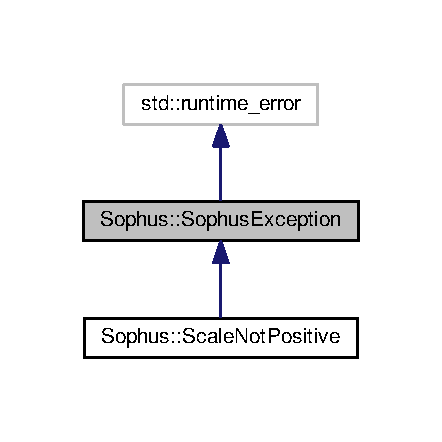
\includegraphics[width=212pt]{class_sophus_1_1_sophus_exception__inherit__graph}
\end{center}
\end{figure}


Collaboration diagram for Sophus\+:\+:Sophus\+Exception\+:
\nopagebreak
\begin{figure}[H]
\begin{center}
\leavevmode
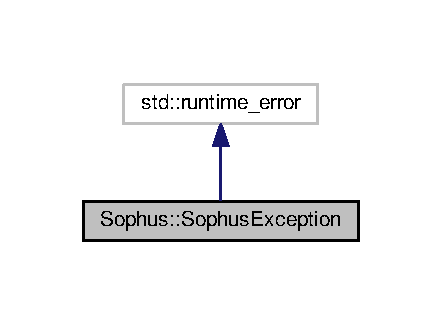
\includegraphics[width=212pt]{class_sophus_1_1_sophus_exception__coll__graph}
\end{center}
\end{figure}
\subsection*{Public Member Functions}
\begin{DoxyCompactItemize}
\item 
{\bfseries Sophus\+Exception} (const std\+::string \&str)\hypertarget{class_sophus_1_1_sophus_exception_a0be113e757a34e37428e52110f565abd}{}\label{class_sophus_1_1_sophus_exception_a0be113e757a34e37428e52110f565abd}

\end{DoxyCompactItemize}


\subsection{Detailed Description}


Definition at line 68 of file sophus.\+hpp.



The documentation for this class was generated from the following file\+:\begin{DoxyCompactItemize}
\item 
include/\+Sophus/sophus/sophus.\+hpp\end{DoxyCompactItemize}

\hypertarget{class_sophus_1_1_tests}{}\section{Sophus\+:\+:Tests$<$ Lie\+Group $>$ Class Template Reference}
\label{class_sophus_1_1_tests}\index{Sophus\+::\+Tests$<$ Lie\+Group $>$@{Sophus\+::\+Tests$<$ Lie\+Group $>$}}
\subsection*{Public Types}
\begin{DoxyCompactItemize}
\item 
typedef Lie\+Group\+::\+Scalar {\bfseries Scalar}\hypertarget{class_sophus_1_1_tests_af59d45a6ee78c8911bb7b4244eec9d86}{}\label{class_sophus_1_1_tests_af59d45a6ee78c8911bb7b4244eec9d86}

\item 
typedef Lie\+Group\+::\+Transformation {\bfseries Transformation}\hypertarget{class_sophus_1_1_tests_adc9997e7b1608b3061a0768bd967f6e3}{}\label{class_sophus_1_1_tests_adc9997e7b1608b3061a0768bd967f6e3}

\item 
typedef Lie\+Group\+::\+Tangent {\bfseries Tangent}\hypertarget{class_sophus_1_1_tests_aecfde8325b438503f13731e5082fdc67}{}\label{class_sophus_1_1_tests_aecfde8325b438503f13731e5082fdc67}

\item 
typedef Lie\+Group\+::\+Point {\bfseries Point}\hypertarget{class_sophus_1_1_tests_a51613730215d694f5c0ac97962131222}{}\label{class_sophus_1_1_tests_a51613730215d694f5c0ac97962131222}

\item 
typedef Lie\+Group\+::\+Adjoint {\bfseries Adjoint}\hypertarget{class_sophus_1_1_tests_aed4d7143d23352dbe8d453daf0316dde}{}\label{class_sophus_1_1_tests_aed4d7143d23352dbe8d453daf0316dde}

\end{DoxyCompactItemize}
\subsection*{Public Member Functions}
\begin{DoxyCompactItemize}
\item 
void {\bfseries set\+Group\+Elements} (const vector$<$ Lie\+Group $>$ \&group\+\_\+vec)\hypertarget{class_sophus_1_1_tests_aa556351b6ec42dbd798ccb2d89d25731}{}\label{class_sophus_1_1_tests_aa556351b6ec42dbd798ccb2d89d25731}

\item 
void {\bfseries set\+Tangent\+Vectors} (const vector$<$ Tangent $>$ \&tangent\+\_\+vec)\hypertarget{class_sophus_1_1_tests_ac56be32b9b622434bbb63daeba0d71f1}{}\label{class_sophus_1_1_tests_ac56be32b9b622434bbb63daeba0d71f1}

\item 
void {\bfseries set\+Points} (const vector$<$ Point $>$ \&point\+\_\+vec)\hypertarget{class_sophus_1_1_tests_a10e71031aad3a2b0f27f3c7e3910795d}{}\label{class_sophus_1_1_tests_a10e71031aad3a2b0f27f3c7e3910795d}

\item 
bool {\bfseries adjoint\+Test} ()\hypertarget{class_sophus_1_1_tests_a6ebb5699c186b1f8131328b61122b072}{}\label{class_sophus_1_1_tests_a6ebb5699c186b1f8131328b61122b072}

\item 
bool {\bfseries exp\+Log\+Test} ()\hypertarget{class_sophus_1_1_tests_adc3dd7283848ee5cb286c33b31555e27}{}\label{class_sophus_1_1_tests_adc3dd7283848ee5cb286c33b31555e27}

\item 
bool {\bfseries exp\+Map\+Test} ()\hypertarget{class_sophus_1_1_tests_a0aefd979ae1d238e5fa9cd0fbd6e8ca2}{}\label{class_sophus_1_1_tests_a0aefd979ae1d238e5fa9cd0fbd6e8ca2}

\item 
bool {\bfseries group\+Action\+Test} ()\hypertarget{class_sophus_1_1_tests_ad70372082f66ff29a4de6a8baec29fad}{}\label{class_sophus_1_1_tests_ad70372082f66ff29a4de6a8baec29fad}

\item 
bool {\bfseries lie\+Bracket\+Test} ()\hypertarget{class_sophus_1_1_tests_a7a2dcafc58820d3148785f90b5506e1b}{}\label{class_sophus_1_1_tests_a7a2dcafc58820d3148785f90b5506e1b}

\item 
bool {\bfseries map\+And\+Mult\+Test} ()\hypertarget{class_sophus_1_1_tests_af3b3f9c4af8180dba91900def4baafb4}{}\label{class_sophus_1_1_tests_af3b3f9c4af8180dba91900def4baafb4}

\item 
bool {\bfseries vee\+Hat\+Test} ()\hypertarget{class_sophus_1_1_tests_af49695637bd2a08bdd2583132c1b4399}{}\label{class_sophus_1_1_tests_af49695637bd2a08bdd2583132c1b4399}

\item 
void {\bfseries run\+All\+Tests} ()\hypertarget{class_sophus_1_1_tests_ae2f469f25d1a7478466480725be2cf97}{}\label{class_sophus_1_1_tests_ae2f469f25d1a7478466480725be2cf97}

\end{DoxyCompactItemize}
\subsection*{Public Attributes}
\begin{DoxyCompactItemize}
\item 
const Scalar {\bfseries S\+M\+A\+L\+L\+\_\+\+E\+PS}\hypertarget{class_sophus_1_1_tests_a439dcadb8477274a0b2ab20f0dbc08d4}{}\label{class_sophus_1_1_tests_a439dcadb8477274a0b2ab20f0dbc08d4}

\end{DoxyCompactItemize}
\subsection*{Static Public Attributes}
\begin{DoxyCompactItemize}
\item 
static const int {\bfseries N} = Lie\+Group\+::N\hypertarget{class_sophus_1_1_tests_a8645b889a8db98096449d75c4bd603a8}{}\label{class_sophus_1_1_tests_a8645b889a8db98096449d75c4bd603a8}

\item 
static const int {\bfseries DoF} = Lie\+Group\+::\+DoF\hypertarget{class_sophus_1_1_tests_adef1c1f22b34d22187aa6838a23bfa41}{}\label{class_sophus_1_1_tests_adef1c1f22b34d22187aa6838a23bfa41}

\end{DoxyCompactItemize}


\subsection{Detailed Description}
\subsubsection*{template$<$class Lie\+Group$>$\\*
class Sophus\+::\+Tests$<$ Lie\+Group $>$}



Definition at line 15 of file tests.\+hpp.



The documentation for this class was generated from the following file\+:\begin{DoxyCompactItemize}
\item 
include/\+Sophus/sophus/tests.\+hpp\end{DoxyCompactItemize}

\hypertarget{struct_eigen_1_1internal_1_1traits_3_01_map_3_01const_01_sophus_1_1_rx_s_o3_group_3_01___scalar_01_4_00_01___options_01_4_01_4}{}\section{Eigen\+:\+:internal\+:\+:traits$<$ Map$<$ const Sophus\+:\+:Rx\+S\+O3\+Group$<$ \+\_\+\+Scalar $>$, \+\_\+\+Options $>$ $>$ Struct Template Reference}
\label{struct_eigen_1_1internal_1_1traits_3_01_map_3_01const_01_sophus_1_1_rx_s_o3_group_3_01___scalar_01_4_00_01___options_01_4_01_4}\index{Eigen\+::internal\+::traits$<$ Map$<$ const Sophus\+::\+Rx\+S\+O3\+Group$<$ \+\_\+\+Scalar $>$, \+\_\+\+Options $>$ $>$@{Eigen\+::internal\+::traits$<$ Map$<$ const Sophus\+::\+Rx\+S\+O3\+Group$<$ \+\_\+\+Scalar $>$, \+\_\+\+Options $>$ $>$}}


Inheritance diagram for Eigen\+:\+:internal\+:\+:traits$<$ Map$<$ const Sophus\+:\+:Rx\+S\+O3\+Group$<$ \+\_\+\+Scalar $>$, \+\_\+\+Options $>$ $>$\+:
\nopagebreak
\begin{figure}[H]
\begin{center}
\leavevmode
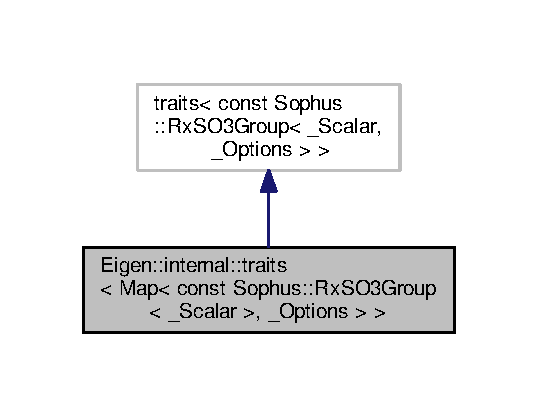
\includegraphics[width=258pt]{struct_eigen_1_1internal_1_1traits_3_01_map_3_01const_01_sophus_1_1_rx_s_o3_group_3_01___scalar_bc2b46e1e30a45ec4fb0b21e26a84111}
\end{center}
\end{figure}


Collaboration diagram for Eigen\+:\+:internal\+:\+:traits$<$ Map$<$ const Sophus\+:\+:Rx\+S\+O3\+Group$<$ \+\_\+\+Scalar $>$, \+\_\+\+Options $>$ $>$\+:
\nopagebreak
\begin{figure}[H]
\begin{center}
\leavevmode
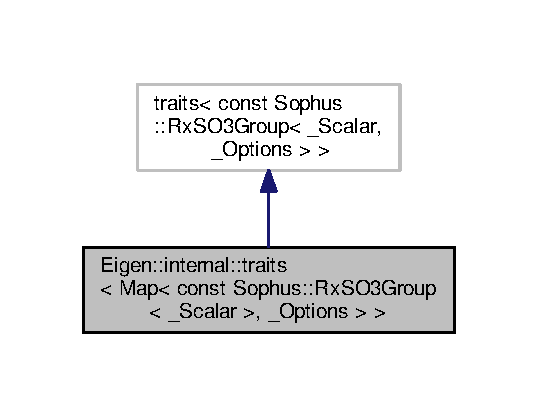
\includegraphics[width=258pt]{struct_eigen_1_1internal_1_1traits_3_01_map_3_01const_01_sophus_1_1_rx_s_o3_group_3_01___scalar_f2f83d8169f5097e8cb7b00197aa71f3}
\end{center}
\end{figure}
\subsection*{Public Types}
\begin{DoxyCompactItemize}
\item 
typedef \+\_\+\+Scalar {\bfseries Scalar}\hypertarget{struct_eigen_1_1internal_1_1traits_3_01_map_3_01const_01_sophus_1_1_rx_s_o3_group_3_01___scalar_01_4_00_01___options_01_4_01_4_a7ec59c13ad809a7568e5bbdef4a8819e}{}\label{struct_eigen_1_1internal_1_1traits_3_01_map_3_01const_01_sophus_1_1_rx_s_o3_group_3_01___scalar_01_4_00_01___options_01_4_01_4_a7ec59c13ad809a7568e5bbdef4a8819e}

\item 
typedef Map$<$ const Quaternion$<$ Scalar $>$, \+\_\+\+Options $>$ {\bfseries Quaternion\+Type}\hypertarget{struct_eigen_1_1internal_1_1traits_3_01_map_3_01const_01_sophus_1_1_rx_s_o3_group_3_01___scalar_01_4_00_01___options_01_4_01_4_af549201042034e5b5a51e8cce11e3bf2}{}\label{struct_eigen_1_1internal_1_1traits_3_01_map_3_01const_01_sophus_1_1_rx_s_o3_group_3_01___scalar_01_4_00_01___options_01_4_01_4_af549201042034e5b5a51e8cce11e3bf2}

\end{DoxyCompactItemize}


\subsection{Detailed Description}
\subsubsection*{template$<$typename \+\_\+\+Scalar, int \+\_\+\+Options$>$\\*
struct Eigen\+::internal\+::traits$<$ Map$<$ const Sophus\+::\+Rx\+S\+O3\+Group$<$ \+\_\+\+Scalar $>$, \+\_\+\+Options $>$ $>$}



Definition at line 61 of file rxso3.\+hpp.



The documentation for this struct was generated from the following file\+:\begin{DoxyCompactItemize}
\item 
include/\+Sophus/sophus/rxso3.\+hpp\end{DoxyCompactItemize}

\hypertarget{struct_eigen_1_1internal_1_1traits_3_01_map_3_01const_01_sophus_1_1_s_e2_group_3_01___scalar_01_4_00_01___options_01_4_01_4}{}\section{Eigen\+:\+:internal\+:\+:traits$<$ Map$<$ const Sophus\+:\+:S\+E2\+Group$<$ \+\_\+\+Scalar $>$, \+\_\+\+Options $>$ $>$ Struct Template Reference}
\label{struct_eigen_1_1internal_1_1traits_3_01_map_3_01const_01_sophus_1_1_s_e2_group_3_01___scalar_01_4_00_01___options_01_4_01_4}\index{Eigen\+::internal\+::traits$<$ Map$<$ const Sophus\+::\+S\+E2\+Group$<$ \+\_\+\+Scalar $>$, \+\_\+\+Options $>$ $>$@{Eigen\+::internal\+::traits$<$ Map$<$ const Sophus\+::\+S\+E2\+Group$<$ \+\_\+\+Scalar $>$, \+\_\+\+Options $>$ $>$}}


Inheritance diagram for Eigen\+:\+:internal\+:\+:traits$<$ Map$<$ const Sophus\+:\+:S\+E2\+Group$<$ \+\_\+\+Scalar $>$, \+\_\+\+Options $>$ $>$\+:
\nopagebreak
\begin{figure}[H]
\begin{center}
\leavevmode
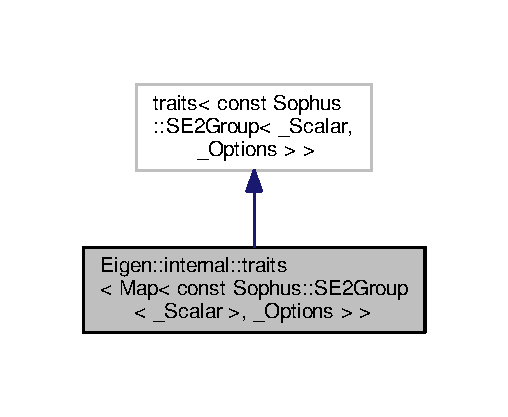
\includegraphics[width=244pt]{struct_eigen_1_1internal_1_1traits_3_01_map_3_01const_01_sophus_1_1_s_e2_group_3_01___scalar_01_9703b4c525ab7a8a6cea3c2724270eec}
\end{center}
\end{figure}


Collaboration diagram for Eigen\+:\+:internal\+:\+:traits$<$ Map$<$ const Sophus\+:\+:S\+E2\+Group$<$ \+\_\+\+Scalar $>$, \+\_\+\+Options $>$ $>$\+:
\nopagebreak
\begin{figure}[H]
\begin{center}
\leavevmode
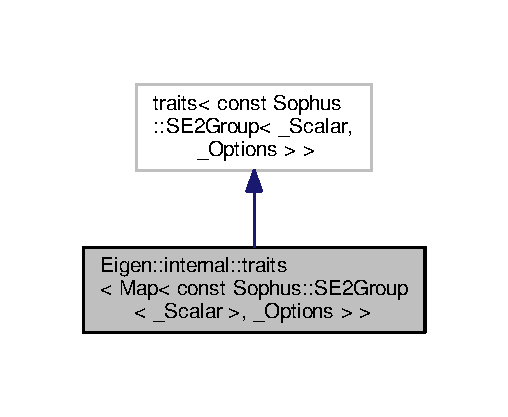
\includegraphics[width=244pt]{struct_eigen_1_1internal_1_1traits_3_01_map_3_01const_01_sophus_1_1_s_e2_group_3_01___scalar_01_ebb9a1e6d28965f31297e7018f0375a3}
\end{center}
\end{figure}
\subsection*{Public Types}
\begin{DoxyCompactItemize}
\item 
typedef \+\_\+\+Scalar {\bfseries Scalar}\hypertarget{struct_eigen_1_1internal_1_1traits_3_01_map_3_01const_01_sophus_1_1_s_e2_group_3_01___scalar_01_4_00_01___options_01_4_01_4_a196ce0a796f33f211b62a518d02bb2ad}{}\label{struct_eigen_1_1internal_1_1traits_3_01_map_3_01const_01_sophus_1_1_s_e2_group_3_01___scalar_01_4_00_01___options_01_4_01_4_a196ce0a796f33f211b62a518d02bb2ad}

\item 
typedef Map$<$ const Matrix$<$ Scalar, 2, 1 $>$, \+\_\+\+Options $>$ {\bfseries Translation\+Type}\hypertarget{struct_eigen_1_1internal_1_1traits_3_01_map_3_01const_01_sophus_1_1_s_e2_group_3_01___scalar_01_4_00_01___options_01_4_01_4_a89ec49a6ef16f42393fe25d22ce2fa43}{}\label{struct_eigen_1_1internal_1_1traits_3_01_map_3_01const_01_sophus_1_1_s_e2_group_3_01___scalar_01_4_00_01___options_01_4_01_4_a89ec49a6ef16f42393fe25d22ce2fa43}

\item 
typedef Map$<$ const \hyperlink{class_sophus_1_1_s_o2_group}{Sophus\+::\+S\+O2\+Group}$<$ Scalar $>$, \+\_\+\+Options $>$ {\bfseries S\+O2\+Type}\hypertarget{struct_eigen_1_1internal_1_1traits_3_01_map_3_01const_01_sophus_1_1_s_e2_group_3_01___scalar_01_4_00_01___options_01_4_01_4_a6712fbc007ed0d62e9bb115cba7e59aa}{}\label{struct_eigen_1_1internal_1_1traits_3_01_map_3_01const_01_sophus_1_1_s_e2_group_3_01___scalar_01_4_00_01___options_01_4_01_4_a6712fbc007ed0d62e9bb115cba7e59aa}

\end{DoxyCompactItemize}


\subsection{Detailed Description}
\subsubsection*{template$<$typename \+\_\+\+Scalar, int \+\_\+\+Options$>$\\*
struct Eigen\+::internal\+::traits$<$ Map$<$ const Sophus\+::\+S\+E2\+Group$<$ \+\_\+\+Scalar $>$, \+\_\+\+Options $>$ $>$}



Definition at line 62 of file se2.\+hpp.



The documentation for this struct was generated from the following file\+:\begin{DoxyCompactItemize}
\item 
include/\+Sophus/sophus/se2.\+hpp\end{DoxyCompactItemize}

\hypertarget{struct_eigen_1_1internal_1_1traits_3_01_map_3_01const_01_sophus_1_1_s_e3_group_3_01___scalar_01_4_00_01___options_01_4_01_4}{}\section{Eigen\+:\+:internal\+:\+:traits$<$ Map$<$ const Sophus\+:\+:S\+E3\+Group$<$ \+\_\+\+Scalar $>$, \+\_\+\+Options $>$ $>$ Struct Template Reference}
\label{struct_eigen_1_1internal_1_1traits_3_01_map_3_01const_01_sophus_1_1_s_e3_group_3_01___scalar_01_4_00_01___options_01_4_01_4}\index{Eigen\+::internal\+::traits$<$ Map$<$ const Sophus\+::\+S\+E3\+Group$<$ \+\_\+\+Scalar $>$, \+\_\+\+Options $>$ $>$@{Eigen\+::internal\+::traits$<$ Map$<$ const Sophus\+::\+S\+E3\+Group$<$ \+\_\+\+Scalar $>$, \+\_\+\+Options $>$ $>$}}


Inheritance diagram for Eigen\+:\+:internal\+:\+:traits$<$ Map$<$ const Sophus\+:\+:S\+E3\+Group$<$ \+\_\+\+Scalar $>$, \+\_\+\+Options $>$ $>$\+:
\nopagebreak
\begin{figure}[H]
\begin{center}
\leavevmode
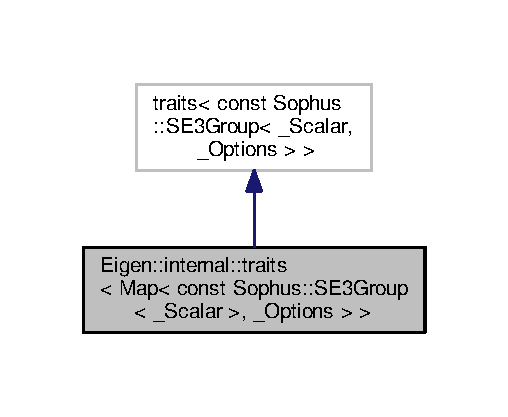
\includegraphics[width=244pt]{struct_eigen_1_1internal_1_1traits_3_01_map_3_01const_01_sophus_1_1_s_e3_group_3_01___scalar_01_52c0efe7410a24c8937f6ba1f1420d56}
\end{center}
\end{figure}


Collaboration diagram for Eigen\+:\+:internal\+:\+:traits$<$ Map$<$ const Sophus\+:\+:S\+E3\+Group$<$ \+\_\+\+Scalar $>$, \+\_\+\+Options $>$ $>$\+:
\nopagebreak
\begin{figure}[H]
\begin{center}
\leavevmode
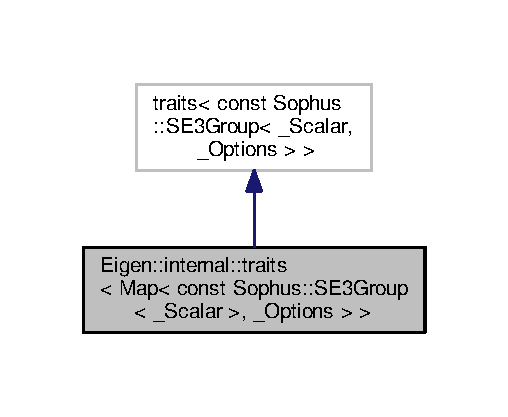
\includegraphics[width=244pt]{struct_eigen_1_1internal_1_1traits_3_01_map_3_01const_01_sophus_1_1_s_e3_group_3_01___scalar_01_b6851729b2a680ef7dff19309b07fdc6}
\end{center}
\end{figure}
\subsection*{Public Types}
\begin{DoxyCompactItemize}
\item 
typedef \+\_\+\+Scalar {\bfseries Scalar}\hypertarget{struct_eigen_1_1internal_1_1traits_3_01_map_3_01const_01_sophus_1_1_s_e3_group_3_01___scalar_01_4_00_01___options_01_4_01_4_a72eaf51cd2fb5a1b7f6bd76aa5ff4920}{}\label{struct_eigen_1_1internal_1_1traits_3_01_map_3_01const_01_sophus_1_1_s_e3_group_3_01___scalar_01_4_00_01___options_01_4_01_4_a72eaf51cd2fb5a1b7f6bd76aa5ff4920}

\item 
typedef Map$<$ const Matrix$<$ Scalar, 3, 1 $>$, \+\_\+\+Options $>$ {\bfseries Translation\+Type}\hypertarget{struct_eigen_1_1internal_1_1traits_3_01_map_3_01const_01_sophus_1_1_s_e3_group_3_01___scalar_01_4_00_01___options_01_4_01_4_a35acc715bfb4969eb792bee9a8bc679b}{}\label{struct_eigen_1_1internal_1_1traits_3_01_map_3_01const_01_sophus_1_1_s_e3_group_3_01___scalar_01_4_00_01___options_01_4_01_4_a35acc715bfb4969eb792bee9a8bc679b}

\item 
typedef Map$<$ const \hyperlink{class_sophus_1_1_s_o3_group}{Sophus\+::\+S\+O3\+Group}$<$ Scalar $>$, \+\_\+\+Options $>$ {\bfseries S\+O3\+Type}\hypertarget{struct_eigen_1_1internal_1_1traits_3_01_map_3_01const_01_sophus_1_1_s_e3_group_3_01___scalar_01_4_00_01___options_01_4_01_4_ae29eef04d53060702010684a505065d7}{}\label{struct_eigen_1_1internal_1_1traits_3_01_map_3_01const_01_sophus_1_1_s_e3_group_3_01___scalar_01_4_00_01___options_01_4_01_4_ae29eef04d53060702010684a505065d7}

\end{DoxyCompactItemize}


\subsection{Detailed Description}
\subsubsection*{template$<$typename \+\_\+\+Scalar, int \+\_\+\+Options$>$\\*
struct Eigen\+::internal\+::traits$<$ Map$<$ const Sophus\+::\+S\+E3\+Group$<$ \+\_\+\+Scalar $>$, \+\_\+\+Options $>$ $>$}



Definition at line 67 of file se3.\+hpp.



The documentation for this struct was generated from the following file\+:\begin{DoxyCompactItemize}
\item 
include/\+Sophus/sophus/se3.\+hpp\end{DoxyCompactItemize}

\hypertarget{struct_eigen_1_1internal_1_1traits_3_01_map_3_01const_01_sophus_1_1_sim3_group_3_01___scalar_01_4_00_01___options_01_4_01_4}{}\section{Eigen\+:\+:internal\+:\+:traits$<$ Map$<$ const Sophus\+:\+:Sim3\+Group$<$ \+\_\+\+Scalar $>$, \+\_\+\+Options $>$ $>$ Struct Template Reference}
\label{struct_eigen_1_1internal_1_1traits_3_01_map_3_01const_01_sophus_1_1_sim3_group_3_01___scalar_01_4_00_01___options_01_4_01_4}\index{Eigen\+::internal\+::traits$<$ Map$<$ const Sophus\+::\+Sim3\+Group$<$ \+\_\+\+Scalar $>$, \+\_\+\+Options $>$ $>$@{Eigen\+::internal\+::traits$<$ Map$<$ const Sophus\+::\+Sim3\+Group$<$ \+\_\+\+Scalar $>$, \+\_\+\+Options $>$ $>$}}


Inheritance diagram for Eigen\+:\+:internal\+:\+:traits$<$ Map$<$ const Sophus\+:\+:Sim3\+Group$<$ \+\_\+\+Scalar $>$, \+\_\+\+Options $>$ $>$\+:
\nopagebreak
\begin{figure}[H]
\begin{center}
\leavevmode
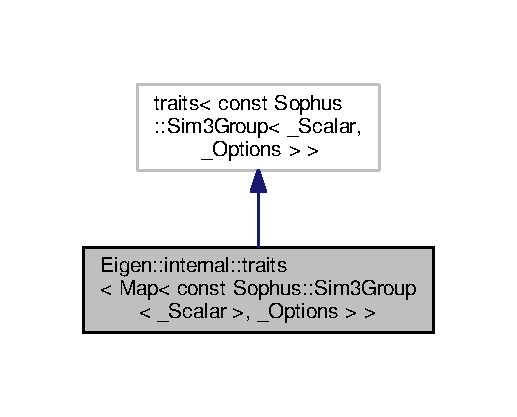
\includegraphics[width=248pt]{struct_eigen_1_1internal_1_1traits_3_01_map_3_01const_01_sophus_1_1_sim3_group_3_01___scalar_01_6359c2cbf8fcc77d54a9a9d69f096544}
\end{center}
\end{figure}


Collaboration diagram for Eigen\+:\+:internal\+:\+:traits$<$ Map$<$ const Sophus\+:\+:Sim3\+Group$<$ \+\_\+\+Scalar $>$, \+\_\+\+Options $>$ $>$\+:
\nopagebreak
\begin{figure}[H]
\begin{center}
\leavevmode
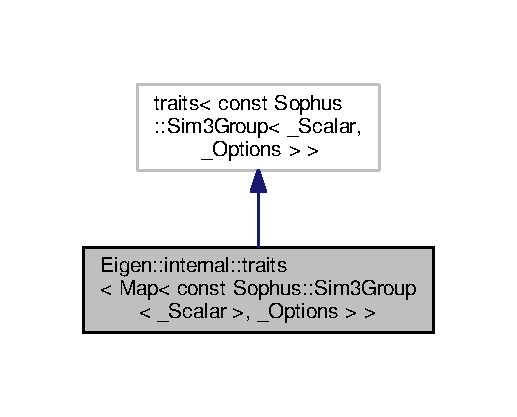
\includegraphics[width=248pt]{struct_eigen_1_1internal_1_1traits_3_01_map_3_01const_01_sophus_1_1_sim3_group_3_01___scalar_01_4099b912049e4b7374d31dd9d38ebf7f}
\end{center}
\end{figure}
\subsection*{Public Types}
\begin{DoxyCompactItemize}
\item 
typedef \+\_\+\+Scalar {\bfseries Scalar}\hypertarget{struct_eigen_1_1internal_1_1traits_3_01_map_3_01const_01_sophus_1_1_sim3_group_3_01___scalar_01_4_00_01___options_01_4_01_4_a16b31ac5dedde7a41bbaa8917ae901cd}{}\label{struct_eigen_1_1internal_1_1traits_3_01_map_3_01const_01_sophus_1_1_sim3_group_3_01___scalar_01_4_00_01___options_01_4_01_4_a16b31ac5dedde7a41bbaa8917ae901cd}

\item 
typedef Map$<$ const Matrix$<$ Scalar, 3, 1 $>$, \+\_\+\+Options $>$ {\bfseries Translation\+Type}\hypertarget{struct_eigen_1_1internal_1_1traits_3_01_map_3_01const_01_sophus_1_1_sim3_group_3_01___scalar_01_4_00_01___options_01_4_01_4_ad8e858a82f8c7f04dcf684d8c536b854}{}\label{struct_eigen_1_1internal_1_1traits_3_01_map_3_01const_01_sophus_1_1_sim3_group_3_01___scalar_01_4_00_01___options_01_4_01_4_ad8e858a82f8c7f04dcf684d8c536b854}

\item 
typedef Map$<$ const \hyperlink{class_sophus_1_1_rx_s_o3_group}{Sophus\+::\+Rx\+S\+O3\+Group}$<$ Scalar $>$, \+\_\+\+Options $>$ {\bfseries Rx\+S\+O3\+Type}\hypertarget{struct_eigen_1_1internal_1_1traits_3_01_map_3_01const_01_sophus_1_1_sim3_group_3_01___scalar_01_4_00_01___options_01_4_01_4_ae49d24c0c32a2912fc43df617eb199da}{}\label{struct_eigen_1_1internal_1_1traits_3_01_map_3_01const_01_sophus_1_1_sim3_group_3_01___scalar_01_4_00_01___options_01_4_01_4_ae49d24c0c32a2912fc43df617eb199da}

\end{DoxyCompactItemize}


\subsection{Detailed Description}
\subsubsection*{template$<$typename \+\_\+\+Scalar, int \+\_\+\+Options$>$\\*
struct Eigen\+::internal\+::traits$<$ Map$<$ const Sophus\+::\+Sim3\+Group$<$ \+\_\+\+Scalar $>$, \+\_\+\+Options $>$ $>$}



Definition at line 66 of file sim3.\+hpp.



The documentation for this struct was generated from the following file\+:\begin{DoxyCompactItemize}
\item 
include/\+Sophus/sophus/sim3.\+hpp\end{DoxyCompactItemize}

\hypertarget{struct_eigen_1_1internal_1_1traits_3_01_map_3_01const_01_sophus_1_1_s_o2_group_3_01___scalar_01_4_00_01___options_01_4_01_4}{}\section{Eigen\+:\+:internal\+:\+:traits$<$ Map$<$ const Sophus\+:\+:S\+O2\+Group$<$ \+\_\+\+Scalar $>$, \+\_\+\+Options $>$ $>$ Struct Template Reference}
\label{struct_eigen_1_1internal_1_1traits_3_01_map_3_01const_01_sophus_1_1_s_o2_group_3_01___scalar_01_4_00_01___options_01_4_01_4}\index{Eigen\+::internal\+::traits$<$ Map$<$ const Sophus\+::\+S\+O2\+Group$<$ \+\_\+\+Scalar $>$, \+\_\+\+Options $>$ $>$@{Eigen\+::internal\+::traits$<$ Map$<$ const Sophus\+::\+S\+O2\+Group$<$ \+\_\+\+Scalar $>$, \+\_\+\+Options $>$ $>$}}


Inheritance diagram for Eigen\+:\+:internal\+:\+:traits$<$ Map$<$ const Sophus\+:\+:S\+O2\+Group$<$ \+\_\+\+Scalar $>$, \+\_\+\+Options $>$ $>$\+:
\nopagebreak
\begin{figure}[H]
\begin{center}
\leavevmode
\includegraphics[width=245pt]{struct_eigen_1_1internal_1_1traits_3_01_map_3_01const_01_sophus_1_1_s_o2_group_3_01___scalar_01_75cb7900d1ac15d034e976b692579c81}
\end{center}
\end{figure}


Collaboration diagram for Eigen\+:\+:internal\+:\+:traits$<$ Map$<$ const Sophus\+:\+:S\+O2\+Group$<$ \+\_\+\+Scalar $>$, \+\_\+\+Options $>$ $>$\+:
\nopagebreak
\begin{figure}[H]
\begin{center}
\leavevmode
\includegraphics[width=245pt]{struct_eigen_1_1internal_1_1traits_3_01_map_3_01const_01_sophus_1_1_s_o2_group_3_01___scalar_01_f3203b9333f1813ea2d82ac40bd58298}
\end{center}
\end{figure}
\subsection*{Public Types}
\begin{DoxyCompactItemize}
\item 
typedef \+\_\+\+Scalar {\bfseries Scalar}\hypertarget{struct_eigen_1_1internal_1_1traits_3_01_map_3_01const_01_sophus_1_1_s_o2_group_3_01___scalar_01_4_00_01___options_01_4_01_4_a4824c3f0c34ba642e1d6443d2374b04f}{}\label{struct_eigen_1_1internal_1_1traits_3_01_map_3_01const_01_sophus_1_1_s_o2_group_3_01___scalar_01_4_00_01___options_01_4_01_4_a4824c3f0c34ba642e1d6443d2374b04f}

\item 
typedef Map$<$ const Matrix$<$ Scalar, 2, 1 $>$, \+\_\+\+Options $>$ {\bfseries Complex\+Type}\hypertarget{struct_eigen_1_1internal_1_1traits_3_01_map_3_01const_01_sophus_1_1_s_o2_group_3_01___scalar_01_4_00_01___options_01_4_01_4_ab4466e39ebed24f825f123878f28a77d}{}\label{struct_eigen_1_1internal_1_1traits_3_01_map_3_01const_01_sophus_1_1_s_o2_group_3_01___scalar_01_4_00_01___options_01_4_01_4_ab4466e39ebed24f825f123878f28a77d}

\end{DoxyCompactItemize}


\subsection{Detailed Description}
\subsubsection*{template$<$typename \+\_\+\+Scalar, int \+\_\+\+Options$>$\\*
struct Eigen\+::internal\+::traits$<$ Map$<$ const Sophus\+::\+S\+O2\+Group$<$ \+\_\+\+Scalar $>$, \+\_\+\+Options $>$ $>$}



Definition at line 66 of file so2.\+hpp.



The documentation for this struct was generated from the following file\+:\begin{DoxyCompactItemize}
\item 
include/\+Sophus/sophus/so2.\+hpp\end{DoxyCompactItemize}

\hypertarget{struct_eigen_1_1internal_1_1traits_3_01_map_3_01const_01_sophus_1_1_s_o3_group_3_01___scalar_01_4_00_01___options_01_4_01_4}{}\section{Eigen\+:\+:internal\+:\+:traits$<$ Map$<$ const Sophus\+:\+:S\+O3\+Group$<$ \+\_\+\+Scalar $>$, \+\_\+\+Options $>$ $>$ Struct Template Reference}
\label{struct_eigen_1_1internal_1_1traits_3_01_map_3_01const_01_sophus_1_1_s_o3_group_3_01___scalar_01_4_00_01___options_01_4_01_4}\index{Eigen\+::internal\+::traits$<$ Map$<$ const Sophus\+::\+S\+O3\+Group$<$ \+\_\+\+Scalar $>$, \+\_\+\+Options $>$ $>$@{Eigen\+::internal\+::traits$<$ Map$<$ const Sophus\+::\+S\+O3\+Group$<$ \+\_\+\+Scalar $>$, \+\_\+\+Options $>$ $>$}}


Inheritance diagram for Eigen\+:\+:internal\+:\+:traits$<$ Map$<$ const Sophus\+:\+:S\+O3\+Group$<$ \+\_\+\+Scalar $>$, \+\_\+\+Options $>$ $>$\+:
\nopagebreak
\begin{figure}[H]
\begin{center}
\leavevmode
\includegraphics[width=245pt]{struct_eigen_1_1internal_1_1traits_3_01_map_3_01const_01_sophus_1_1_s_o3_group_3_01___scalar_01_3fbed213f5b350c4a602acc1636357a2}
\end{center}
\end{figure}


Collaboration diagram for Eigen\+:\+:internal\+:\+:traits$<$ Map$<$ const Sophus\+:\+:S\+O3\+Group$<$ \+\_\+\+Scalar $>$, \+\_\+\+Options $>$ $>$\+:
\nopagebreak
\begin{figure}[H]
\begin{center}
\leavevmode
\includegraphics[width=245pt]{struct_eigen_1_1internal_1_1traits_3_01_map_3_01const_01_sophus_1_1_s_o3_group_3_01___scalar_01_fcaf1bfa9f755c257921a0a3fd6432be}
\end{center}
\end{figure}
\subsection*{Public Types}
\begin{DoxyCompactItemize}
\item 
typedef \+\_\+\+Scalar {\bfseries Scalar}\hypertarget{struct_eigen_1_1internal_1_1traits_3_01_map_3_01const_01_sophus_1_1_s_o3_group_3_01___scalar_01_4_00_01___options_01_4_01_4_a08dbe18456b568af29d3c3548307d106}{}\label{struct_eigen_1_1internal_1_1traits_3_01_map_3_01const_01_sophus_1_1_s_o3_group_3_01___scalar_01_4_00_01___options_01_4_01_4_a08dbe18456b568af29d3c3548307d106}

\item 
typedef Map$<$ const Quaternion$<$ Scalar $>$, \+\_\+\+Options $>$ {\bfseries Quaternion\+Type}\hypertarget{struct_eigen_1_1internal_1_1traits_3_01_map_3_01const_01_sophus_1_1_s_o3_group_3_01___scalar_01_4_00_01___options_01_4_01_4_a5a6d66441e7043e0b26514632be9b9cf}{}\label{struct_eigen_1_1internal_1_1traits_3_01_map_3_01const_01_sophus_1_1_s_o3_group_3_01___scalar_01_4_00_01___options_01_4_01_4_a5a6d66441e7043e0b26514632be9b9cf}

\end{DoxyCompactItemize}


\subsection{Detailed Description}
\subsubsection*{template$<$typename \+\_\+\+Scalar, int \+\_\+\+Options$>$\\*
struct Eigen\+::internal\+::traits$<$ Map$<$ const Sophus\+::\+S\+O3\+Group$<$ \+\_\+\+Scalar $>$, \+\_\+\+Options $>$ $>$}



Definition at line 61 of file so3.\+hpp.



The documentation for this struct was generated from the following file\+:\begin{DoxyCompactItemize}
\item 
include/\+Sophus/sophus/so3.\+hpp\end{DoxyCompactItemize}

\hypertarget{struct_eigen_1_1internal_1_1traits_3_01_map_3_01_sophus_1_1_rx_s_o3_group_3_01___scalar_01_4_00_01___options_01_4_01_4}{}\section{Eigen\+:\+:internal\+:\+:traits$<$ Map$<$ Sophus\+:\+:Rx\+S\+O3\+Group$<$ \+\_\+\+Scalar $>$, \+\_\+\+Options $>$ $>$ Struct Template Reference}
\label{struct_eigen_1_1internal_1_1traits_3_01_map_3_01_sophus_1_1_rx_s_o3_group_3_01___scalar_01_4_00_01___options_01_4_01_4}\index{Eigen\+::internal\+::traits$<$ Map$<$ Sophus\+::\+Rx\+S\+O3\+Group$<$ \+\_\+\+Scalar $>$, \+\_\+\+Options $>$ $>$@{Eigen\+::internal\+::traits$<$ Map$<$ Sophus\+::\+Rx\+S\+O3\+Group$<$ \+\_\+\+Scalar $>$, \+\_\+\+Options $>$ $>$}}


Inheritance diagram for Eigen\+:\+:internal\+:\+:traits$<$ Map$<$ Sophus\+:\+:Rx\+S\+O3\+Group$<$ \+\_\+\+Scalar $>$, \+\_\+\+Options $>$ $>$\+:
\nopagebreak
\begin{figure}[H]
\begin{center}
\leavevmode
\includegraphics[width=231pt]{struct_eigen_1_1internal_1_1traits_3_01_map_3_01_sophus_1_1_rx_s_o3_group_3_01___scalar_01_4_00_7550b7457758b50dc514ea3270050fb7}
\end{center}
\end{figure}


Collaboration diagram for Eigen\+:\+:internal\+:\+:traits$<$ Map$<$ Sophus\+:\+:Rx\+S\+O3\+Group$<$ \+\_\+\+Scalar $>$, \+\_\+\+Options $>$ $>$\+:
\nopagebreak
\begin{figure}[H]
\begin{center}
\leavevmode
\includegraphics[width=231pt]{struct_eigen_1_1internal_1_1traits_3_01_map_3_01_sophus_1_1_rx_s_o3_group_3_01___scalar_01_4_00_3fd307b06f7ae7f0244bbc8eeb5f035e}
\end{center}
\end{figure}
\subsection*{Public Types}
\begin{DoxyCompactItemize}
\item 
typedef \+\_\+\+Scalar {\bfseries Scalar}\hypertarget{struct_eigen_1_1internal_1_1traits_3_01_map_3_01_sophus_1_1_rx_s_o3_group_3_01___scalar_01_4_00_01___options_01_4_01_4_a154ccaa06c68bd744ad4b625d3faa791}{}\label{struct_eigen_1_1internal_1_1traits_3_01_map_3_01_sophus_1_1_rx_s_o3_group_3_01___scalar_01_4_00_01___options_01_4_01_4_a154ccaa06c68bd744ad4b625d3faa791}

\item 
typedef Map$<$ Quaternion$<$ Scalar $>$, \+\_\+\+Options $>$ {\bfseries Quaternion\+Type}\hypertarget{struct_eigen_1_1internal_1_1traits_3_01_map_3_01_sophus_1_1_rx_s_o3_group_3_01___scalar_01_4_00_01___options_01_4_01_4_a5509a89c29e9b459ad066ea17f2ef931}{}\label{struct_eigen_1_1internal_1_1traits_3_01_map_3_01_sophus_1_1_rx_s_o3_group_3_01___scalar_01_4_00_01___options_01_4_01_4_a5509a89c29e9b459ad066ea17f2ef931}

\end{DoxyCompactItemize}


\subsection{Detailed Description}
\subsubsection*{template$<$typename \+\_\+\+Scalar, int \+\_\+\+Options$>$\\*
struct Eigen\+::internal\+::traits$<$ Map$<$ Sophus\+::\+Rx\+S\+O3\+Group$<$ \+\_\+\+Scalar $>$, \+\_\+\+Options $>$ $>$}



Definition at line 54 of file rxso3.\+hpp.



The documentation for this struct was generated from the following file\+:\begin{DoxyCompactItemize}
\item 
include/\+Sophus/sophus/rxso3.\+hpp\end{DoxyCompactItemize}

\hypertarget{struct_eigen_1_1internal_1_1traits_3_01_map_3_01_sophus_1_1_s_e2_group_3_01___scalar_01_4_00_01___options_01_4_01_4}{}\section{Eigen\+:\+:internal\+:\+:traits$<$ Map$<$ Sophus\+:\+:S\+E2\+Group$<$ \+\_\+\+Scalar $>$, \+\_\+\+Options $>$ $>$ Struct Template Reference}
\label{struct_eigen_1_1internal_1_1traits_3_01_map_3_01_sophus_1_1_s_e2_group_3_01___scalar_01_4_00_01___options_01_4_01_4}\index{Eigen\+::internal\+::traits$<$ Map$<$ Sophus\+::\+S\+E2\+Group$<$ \+\_\+\+Scalar $>$, \+\_\+\+Options $>$ $>$@{Eigen\+::internal\+::traits$<$ Map$<$ Sophus\+::\+S\+E2\+Group$<$ \+\_\+\+Scalar $>$, \+\_\+\+Options $>$ $>$}}


Inheritance diagram for Eigen\+:\+:internal\+:\+:traits$<$ Map$<$ Sophus\+:\+:S\+E2\+Group$<$ \+\_\+\+Scalar $>$, \+\_\+\+Options $>$ $>$\+:
\nopagebreak
\begin{figure}[H]
\begin{center}
\leavevmode
\includegraphics[width=235pt]{struct_eigen_1_1internal_1_1traits_3_01_map_3_01_sophus_1_1_s_e2_group_3_01___scalar_01_4_00_01_810fbac80203e679e65324f0ff2e4255}
\end{center}
\end{figure}


Collaboration diagram for Eigen\+:\+:internal\+:\+:traits$<$ Map$<$ Sophus\+:\+:S\+E2\+Group$<$ \+\_\+\+Scalar $>$, \+\_\+\+Options $>$ $>$\+:
\nopagebreak
\begin{figure}[H]
\begin{center}
\leavevmode
\includegraphics[width=235pt]{struct_eigen_1_1internal_1_1traits_3_01_map_3_01_sophus_1_1_s_e2_group_3_01___scalar_01_4_00_01_aa767b2a9f583195514bf750c40a08d4}
\end{center}
\end{figure}
\subsection*{Public Types}
\begin{DoxyCompactItemize}
\item 
typedef \+\_\+\+Scalar {\bfseries Scalar}\hypertarget{struct_eigen_1_1internal_1_1traits_3_01_map_3_01_sophus_1_1_s_e2_group_3_01___scalar_01_4_00_01___options_01_4_01_4_a831a2d38ef48b2ecb345d43f58ce1477}{}\label{struct_eigen_1_1internal_1_1traits_3_01_map_3_01_sophus_1_1_s_e2_group_3_01___scalar_01_4_00_01___options_01_4_01_4_a831a2d38ef48b2ecb345d43f58ce1477}

\item 
typedef Map$<$ Matrix$<$ Scalar, 2, 1 $>$, \+\_\+\+Options $>$ {\bfseries Translation\+Type}\hypertarget{struct_eigen_1_1internal_1_1traits_3_01_map_3_01_sophus_1_1_s_e2_group_3_01___scalar_01_4_00_01___options_01_4_01_4_ae36348f3d5d8e9abb291d4ec09967e34}{}\label{struct_eigen_1_1internal_1_1traits_3_01_map_3_01_sophus_1_1_s_e2_group_3_01___scalar_01_4_00_01___options_01_4_01_4_ae36348f3d5d8e9abb291d4ec09967e34}

\item 
typedef Map$<$ \hyperlink{class_sophus_1_1_s_o2_group}{Sophus\+::\+S\+O2\+Group}$<$ Scalar $>$, \+\_\+\+Options $>$ {\bfseries S\+O2\+Type}\hypertarget{struct_eigen_1_1internal_1_1traits_3_01_map_3_01_sophus_1_1_s_e2_group_3_01___scalar_01_4_00_01___options_01_4_01_4_ae915b7930e5ea24556663518837d9a5c}{}\label{struct_eigen_1_1internal_1_1traits_3_01_map_3_01_sophus_1_1_s_e2_group_3_01___scalar_01_4_00_01___options_01_4_01_4_ae915b7930e5ea24556663518837d9a5c}

\end{DoxyCompactItemize}


\subsection{Detailed Description}
\subsubsection*{template$<$typename \+\_\+\+Scalar, int \+\_\+\+Options$>$\\*
struct Eigen\+::internal\+::traits$<$ Map$<$ Sophus\+::\+S\+E2\+Group$<$ \+\_\+\+Scalar $>$, \+\_\+\+Options $>$ $>$}



Definition at line 54 of file se2.\+hpp.



The documentation for this struct was generated from the following file\+:\begin{DoxyCompactItemize}
\item 
include/\+Sophus/sophus/se2.\+hpp\end{DoxyCompactItemize}

\hypertarget{struct_eigen_1_1internal_1_1traits_3_01_map_3_01_sophus_1_1_s_e3_group_3_01___scalar_01_4_00_01___options_01_4_01_4}{}\section{Eigen\+:\+:internal\+:\+:traits$<$ Map$<$ Sophus\+:\+:S\+E3\+Group$<$ \+\_\+\+Scalar $>$, \+\_\+\+Options $>$ $>$ Struct Template Reference}
\label{struct_eigen_1_1internal_1_1traits_3_01_map_3_01_sophus_1_1_s_e3_group_3_01___scalar_01_4_00_01___options_01_4_01_4}\index{Eigen\+::internal\+::traits$<$ Map$<$ Sophus\+::\+S\+E3\+Group$<$ \+\_\+\+Scalar $>$, \+\_\+\+Options $>$ $>$@{Eigen\+::internal\+::traits$<$ Map$<$ Sophus\+::\+S\+E3\+Group$<$ \+\_\+\+Scalar $>$, \+\_\+\+Options $>$ $>$}}


Inheritance diagram for Eigen\+:\+:internal\+:\+:traits$<$ Map$<$ Sophus\+:\+:S\+E3\+Group$<$ \+\_\+\+Scalar $>$, \+\_\+\+Options $>$ $>$\+:
\nopagebreak
\begin{figure}[H]
\begin{center}
\leavevmode
\includegraphics[width=235pt]{struct_eigen_1_1internal_1_1traits_3_01_map_3_01_sophus_1_1_s_e3_group_3_01___scalar_01_4_00_01_7c582174955688be9f4d161a19f89577}
\end{center}
\end{figure}


Collaboration diagram for Eigen\+:\+:internal\+:\+:traits$<$ Map$<$ Sophus\+:\+:S\+E3\+Group$<$ \+\_\+\+Scalar $>$, \+\_\+\+Options $>$ $>$\+:
\nopagebreak
\begin{figure}[H]
\begin{center}
\leavevmode
\includegraphics[width=235pt]{struct_eigen_1_1internal_1_1traits_3_01_map_3_01_sophus_1_1_s_e3_group_3_01___scalar_01_4_00_01_2a0483a3750a0ceb59dc03e56a24ed74}
\end{center}
\end{figure}
\subsection*{Public Types}
\begin{DoxyCompactItemize}
\item 
typedef \+\_\+\+Scalar {\bfseries Scalar}\hypertarget{struct_eigen_1_1internal_1_1traits_3_01_map_3_01_sophus_1_1_s_e3_group_3_01___scalar_01_4_00_01___options_01_4_01_4_a00a43c378601d006c2b1200a303289a1}{}\label{struct_eigen_1_1internal_1_1traits_3_01_map_3_01_sophus_1_1_s_e3_group_3_01___scalar_01_4_00_01___options_01_4_01_4_a00a43c378601d006c2b1200a303289a1}

\item 
typedef Map$<$ Matrix$<$ Scalar, 3, 1 $>$, \+\_\+\+Options $>$ {\bfseries Translation\+Type}\hypertarget{struct_eigen_1_1internal_1_1traits_3_01_map_3_01_sophus_1_1_s_e3_group_3_01___scalar_01_4_00_01___options_01_4_01_4_a0b153a0b93d8eb3299e3958e2ce5c938}{}\label{struct_eigen_1_1internal_1_1traits_3_01_map_3_01_sophus_1_1_s_e3_group_3_01___scalar_01_4_00_01___options_01_4_01_4_a0b153a0b93d8eb3299e3958e2ce5c938}

\item 
typedef Map$<$ \hyperlink{class_sophus_1_1_s_o3_group}{Sophus\+::\+S\+O3\+Group}$<$ Scalar $>$, \+\_\+\+Options $>$ {\bfseries S\+O3\+Type}\hypertarget{struct_eigen_1_1internal_1_1traits_3_01_map_3_01_sophus_1_1_s_e3_group_3_01___scalar_01_4_00_01___options_01_4_01_4_a85702dd0a64aa4c2db7b7c04f007648b}{}\label{struct_eigen_1_1internal_1_1traits_3_01_map_3_01_sophus_1_1_s_e3_group_3_01___scalar_01_4_00_01___options_01_4_01_4_a85702dd0a64aa4c2db7b7c04f007648b}

\end{DoxyCompactItemize}


\subsection{Detailed Description}
\subsubsection*{template$<$typename \+\_\+\+Scalar, int \+\_\+\+Options$>$\\*
struct Eigen\+::internal\+::traits$<$ Map$<$ Sophus\+::\+S\+E3\+Group$<$ \+\_\+\+Scalar $>$, \+\_\+\+Options $>$ $>$}



Definition at line 59 of file se3.\+hpp.



The documentation for this struct was generated from the following file\+:\begin{DoxyCompactItemize}
\item 
include/\+Sophus/sophus/se3.\+hpp\end{DoxyCompactItemize}

\hypertarget{struct_eigen_1_1internal_1_1traits_3_01_map_3_01_sophus_1_1_sim3_group_3_01___scalar_01_4_00_01___options_01_4_01_4}{}\section{Eigen\+:\+:internal\+:\+:traits$<$ Map$<$ Sophus\+:\+:Sim3\+Group$<$ \+\_\+\+Scalar $>$, \+\_\+\+Options $>$ $>$ Struct Template Reference}
\label{struct_eigen_1_1internal_1_1traits_3_01_map_3_01_sophus_1_1_sim3_group_3_01___scalar_01_4_00_01___options_01_4_01_4}\index{Eigen\+::internal\+::traits$<$ Map$<$ Sophus\+::\+Sim3\+Group$<$ \+\_\+\+Scalar $>$, \+\_\+\+Options $>$ $>$@{Eigen\+::internal\+::traits$<$ Map$<$ Sophus\+::\+Sim3\+Group$<$ \+\_\+\+Scalar $>$, \+\_\+\+Options $>$ $>$}}


Inheritance diagram for Eigen\+:\+:internal\+:\+:traits$<$ Map$<$ Sophus\+:\+:Sim3\+Group$<$ \+\_\+\+Scalar $>$, \+\_\+\+Options $>$ $>$\+:
\nopagebreak
\begin{figure}[H]
\begin{center}
\leavevmode
\includegraphics[width=221pt]{struct_eigen_1_1internal_1_1traits_3_01_map_3_01_sophus_1_1_sim3_group_3_01___scalar_01_4_00_01_1de7e4eff97b0c568bd49784f0f8ff30}
\end{center}
\end{figure}


Collaboration diagram for Eigen\+:\+:internal\+:\+:traits$<$ Map$<$ Sophus\+:\+:Sim3\+Group$<$ \+\_\+\+Scalar $>$, \+\_\+\+Options $>$ $>$\+:
\nopagebreak
\begin{figure}[H]
\begin{center}
\leavevmode
\includegraphics[width=221pt]{struct_eigen_1_1internal_1_1traits_3_01_map_3_01_sophus_1_1_sim3_group_3_01___scalar_01_4_00_01_48dec31b44a7e1dd9f2cb942569b6e43}
\end{center}
\end{figure}
\subsection*{Public Types}
\begin{DoxyCompactItemize}
\item 
typedef \+\_\+\+Scalar {\bfseries Scalar}\hypertarget{struct_eigen_1_1internal_1_1traits_3_01_map_3_01_sophus_1_1_sim3_group_3_01___scalar_01_4_00_01___options_01_4_01_4_afcd1cb515492262eccb85f1e79b1118a}{}\label{struct_eigen_1_1internal_1_1traits_3_01_map_3_01_sophus_1_1_sim3_group_3_01___scalar_01_4_00_01___options_01_4_01_4_afcd1cb515492262eccb85f1e79b1118a}

\item 
typedef Map$<$ Matrix$<$ Scalar, 3, 1 $>$, \+\_\+\+Options $>$ {\bfseries Translation\+Type}\hypertarget{struct_eigen_1_1internal_1_1traits_3_01_map_3_01_sophus_1_1_sim3_group_3_01___scalar_01_4_00_01___options_01_4_01_4_a221f209e15bfcbdb266b363488dbe4d1}{}\label{struct_eigen_1_1internal_1_1traits_3_01_map_3_01_sophus_1_1_sim3_group_3_01___scalar_01_4_00_01___options_01_4_01_4_a221f209e15bfcbdb266b363488dbe4d1}

\item 
typedef Map$<$ \hyperlink{class_sophus_1_1_rx_s_o3_group}{Sophus\+::\+Rx\+S\+O3\+Group}$<$ Scalar $>$, \+\_\+\+Options $>$ {\bfseries Rx\+S\+O3\+Type}\hypertarget{struct_eigen_1_1internal_1_1traits_3_01_map_3_01_sophus_1_1_sim3_group_3_01___scalar_01_4_00_01___options_01_4_01_4_a805b8b91d146515bf0895eeffc26fce5}{}\label{struct_eigen_1_1internal_1_1traits_3_01_map_3_01_sophus_1_1_sim3_group_3_01___scalar_01_4_00_01___options_01_4_01_4_a805b8b91d146515bf0895eeffc26fce5}

\end{DoxyCompactItemize}


\subsection{Detailed Description}
\subsubsection*{template$<$typename \+\_\+\+Scalar, int \+\_\+\+Options$>$\\*
struct Eigen\+::internal\+::traits$<$ Map$<$ Sophus\+::\+Sim3\+Group$<$ \+\_\+\+Scalar $>$, \+\_\+\+Options $>$ $>$}



Definition at line 58 of file sim3.\+hpp.



The documentation for this struct was generated from the following file\+:\begin{DoxyCompactItemize}
\item 
include/\+Sophus/sophus/sim3.\+hpp\end{DoxyCompactItemize}

\hypertarget{struct_eigen_1_1internal_1_1traits_3_01_map_3_01_sophus_1_1_s_o2_group_3_01___scalar_01_4_00_01___options_01_4_01_4}{}\section{Eigen\+:\+:internal\+:\+:traits$<$ Map$<$ Sophus\+:\+:S\+O2\+Group$<$ \+\_\+\+Scalar $>$, \+\_\+\+Options $>$ $>$ Struct Template Reference}
\label{struct_eigen_1_1internal_1_1traits_3_01_map_3_01_sophus_1_1_s_o2_group_3_01___scalar_01_4_00_01___options_01_4_01_4}\index{Eigen\+::internal\+::traits$<$ Map$<$ Sophus\+::\+S\+O2\+Group$<$ \+\_\+\+Scalar $>$, \+\_\+\+Options $>$ $>$@{Eigen\+::internal\+::traits$<$ Map$<$ Sophus\+::\+S\+O2\+Group$<$ \+\_\+\+Scalar $>$, \+\_\+\+Options $>$ $>$}}


Inheritance diagram for Eigen\+:\+:internal\+:\+:traits$<$ Map$<$ Sophus\+:\+:S\+O2\+Group$<$ \+\_\+\+Scalar $>$, \+\_\+\+Options $>$ $>$\+:
\nopagebreak
\begin{figure}[H]
\begin{center}
\leavevmode
\includegraphics[width=235pt]{struct_eigen_1_1internal_1_1traits_3_01_map_3_01_sophus_1_1_s_o2_group_3_01___scalar_01_4_00_01_bf56f312ddf275fb7036c655b98f5183}
\end{center}
\end{figure}


Collaboration diagram for Eigen\+:\+:internal\+:\+:traits$<$ Map$<$ Sophus\+:\+:S\+O2\+Group$<$ \+\_\+\+Scalar $>$, \+\_\+\+Options $>$ $>$\+:
\nopagebreak
\begin{figure}[H]
\begin{center}
\leavevmode
\includegraphics[width=235pt]{struct_eigen_1_1internal_1_1traits_3_01_map_3_01_sophus_1_1_s_o2_group_3_01___scalar_01_4_00_01_7195f98ff6afc2a2016e754beff77e35}
\end{center}
\end{figure}
\subsection*{Public Types}
\begin{DoxyCompactItemize}
\item 
typedef \+\_\+\+Scalar {\bfseries Scalar}\hypertarget{struct_eigen_1_1internal_1_1traits_3_01_map_3_01_sophus_1_1_s_o2_group_3_01___scalar_01_4_00_01___options_01_4_01_4_a439c80ff12c86be62ec6664d13491d8e}{}\label{struct_eigen_1_1internal_1_1traits_3_01_map_3_01_sophus_1_1_s_o2_group_3_01___scalar_01_4_00_01___options_01_4_01_4_a439c80ff12c86be62ec6664d13491d8e}

\item 
typedef Map$<$ Matrix$<$ Scalar, 2, 1 $>$, \+\_\+\+Options $>$ {\bfseries Complex\+Type}\hypertarget{struct_eigen_1_1internal_1_1traits_3_01_map_3_01_sophus_1_1_s_o2_group_3_01___scalar_01_4_00_01___options_01_4_01_4_a020c05fa1834097b5a4e450d89fc40e0}{}\label{struct_eigen_1_1internal_1_1traits_3_01_map_3_01_sophus_1_1_s_o2_group_3_01___scalar_01_4_00_01___options_01_4_01_4_a020c05fa1834097b5a4e450d89fc40e0}

\end{DoxyCompactItemize}


\subsection{Detailed Description}
\subsubsection*{template$<$typename \+\_\+\+Scalar, int \+\_\+\+Options$>$\\*
struct Eigen\+::internal\+::traits$<$ Map$<$ Sophus\+::\+S\+O2\+Group$<$ \+\_\+\+Scalar $>$, \+\_\+\+Options $>$ $>$}



Definition at line 59 of file so2.\+hpp.



The documentation for this struct was generated from the following file\+:\begin{DoxyCompactItemize}
\item 
include/\+Sophus/sophus/so2.\+hpp\end{DoxyCompactItemize}

\hypertarget{struct_eigen_1_1internal_1_1traits_3_01_map_3_01_sophus_1_1_s_o3_group_3_01___scalar_01_4_00_01___options_01_4_01_4}{}\section{Eigen\+:\+:internal\+:\+:traits$<$ Map$<$ Sophus\+:\+:S\+O3\+Group$<$ \+\_\+\+Scalar $>$, \+\_\+\+Options $>$ $>$ Struct Template Reference}
\label{struct_eigen_1_1internal_1_1traits_3_01_map_3_01_sophus_1_1_s_o3_group_3_01___scalar_01_4_00_01___options_01_4_01_4}\index{Eigen\+::internal\+::traits$<$ Map$<$ Sophus\+::\+S\+O3\+Group$<$ \+\_\+\+Scalar $>$, \+\_\+\+Options $>$ $>$@{Eigen\+::internal\+::traits$<$ Map$<$ Sophus\+::\+S\+O3\+Group$<$ \+\_\+\+Scalar $>$, \+\_\+\+Options $>$ $>$}}


Inheritance diagram for Eigen\+:\+:internal\+:\+:traits$<$ Map$<$ Sophus\+:\+:S\+O3\+Group$<$ \+\_\+\+Scalar $>$, \+\_\+\+Options $>$ $>$\+:
\nopagebreak
\begin{figure}[H]
\begin{center}
\leavevmode
\includegraphics[width=235pt]{struct_eigen_1_1internal_1_1traits_3_01_map_3_01_sophus_1_1_s_o3_group_3_01___scalar_01_4_00_01_0329c94ee5f31c540202b49673be2390}
\end{center}
\end{figure}


Collaboration diagram for Eigen\+:\+:internal\+:\+:traits$<$ Map$<$ Sophus\+:\+:S\+O3\+Group$<$ \+\_\+\+Scalar $>$, \+\_\+\+Options $>$ $>$\+:
\nopagebreak
\begin{figure}[H]
\begin{center}
\leavevmode
\includegraphics[width=235pt]{struct_eigen_1_1internal_1_1traits_3_01_map_3_01_sophus_1_1_s_o3_group_3_01___scalar_01_4_00_01_d8eb6d87ccab4c92b994c86e08d5a55f}
\end{center}
\end{figure}
\subsection*{Public Types}
\begin{DoxyCompactItemize}
\item 
typedef \+\_\+\+Scalar {\bfseries Scalar}\hypertarget{struct_eigen_1_1internal_1_1traits_3_01_map_3_01_sophus_1_1_s_o3_group_3_01___scalar_01_4_00_01___options_01_4_01_4_a28eff2bf15b05221714925b13d0a1ad4}{}\label{struct_eigen_1_1internal_1_1traits_3_01_map_3_01_sophus_1_1_s_o3_group_3_01___scalar_01_4_00_01___options_01_4_01_4_a28eff2bf15b05221714925b13d0a1ad4}

\item 
typedef Map$<$ Quaternion$<$ Scalar $>$, \+\_\+\+Options $>$ {\bfseries Quaternion\+Type}\hypertarget{struct_eigen_1_1internal_1_1traits_3_01_map_3_01_sophus_1_1_s_o3_group_3_01___scalar_01_4_00_01___options_01_4_01_4_a1045cb02afb45f2c092a98d65bbee511}{}\label{struct_eigen_1_1internal_1_1traits_3_01_map_3_01_sophus_1_1_s_o3_group_3_01___scalar_01_4_00_01___options_01_4_01_4_a1045cb02afb45f2c092a98d65bbee511}

\end{DoxyCompactItemize}


\subsection{Detailed Description}
\subsubsection*{template$<$typename \+\_\+\+Scalar, int \+\_\+\+Options$>$\\*
struct Eigen\+::internal\+::traits$<$ Map$<$ Sophus\+::\+S\+O3\+Group$<$ \+\_\+\+Scalar $>$, \+\_\+\+Options $>$ $>$}



Definition at line 54 of file so3.\+hpp.



The documentation for this struct was generated from the following file\+:\begin{DoxyCompactItemize}
\item 
include/\+Sophus/sophus/so3.\+hpp\end{DoxyCompactItemize}

\hypertarget{struct_eigen_1_1internal_1_1traits_3_01_sophus_1_1_rx_s_o3_group_3_01___scalar_00_01___options_01_4_01_4}{}\section{Eigen\+:\+:internal\+:\+:traits$<$ Sophus\+:\+:Rx\+S\+O3\+Group$<$ \+\_\+\+Scalar, \+\_\+\+Options $>$ $>$ Struct Template Reference}
\label{struct_eigen_1_1internal_1_1traits_3_01_sophus_1_1_rx_s_o3_group_3_01___scalar_00_01___options_01_4_01_4}\index{Eigen\+::internal\+::traits$<$ Sophus\+::\+Rx\+S\+O3\+Group$<$ \+\_\+\+Scalar, \+\_\+\+Options $>$ $>$@{Eigen\+::internal\+::traits$<$ Sophus\+::\+Rx\+S\+O3\+Group$<$ \+\_\+\+Scalar, \+\_\+\+Options $>$ $>$}}


Inheritance diagram for Eigen\+:\+:internal\+:\+:traits$<$ Sophus\+:\+:Rx\+S\+O3\+Group$<$ \+\_\+\+Scalar, \+\_\+\+Options $>$ $>$\+:
\nopagebreak
\begin{figure}[H]
\begin{center}
\leavevmode
\includegraphics[width=231pt]{struct_eigen_1_1internal_1_1traits_3_01_sophus_1_1_rx_s_o3_group_3_01___scalar_00_01___options_01_4_01_4__inherit__graph}
\end{center}
\end{figure}
\subsection*{Public Types}
\begin{DoxyCompactItemize}
\item 
typedef \+\_\+\+Scalar {\bfseries Scalar}\hypertarget{struct_eigen_1_1internal_1_1traits_3_01_sophus_1_1_rx_s_o3_group_3_01___scalar_00_01___options_01_4_01_4_a0e0d77361db8041b68303f4da97c6309}{}\label{struct_eigen_1_1internal_1_1traits_3_01_sophus_1_1_rx_s_o3_group_3_01___scalar_00_01___options_01_4_01_4_a0e0d77361db8041b68303f4da97c6309}

\item 
typedef Quaternion$<$ Scalar $>$ {\bfseries Quaternion\+Type}\hypertarget{struct_eigen_1_1internal_1_1traits_3_01_sophus_1_1_rx_s_o3_group_3_01___scalar_00_01___options_01_4_01_4_ab699bd038a65bf712da4d899b90738e0}{}\label{struct_eigen_1_1internal_1_1traits_3_01_sophus_1_1_rx_s_o3_group_3_01___scalar_00_01___options_01_4_01_4_ab699bd038a65bf712da4d899b90738e0}

\end{DoxyCompactItemize}


\subsection{Detailed Description}
\subsubsection*{template$<$typename \+\_\+\+Scalar, int \+\_\+\+Options$>$\\*
struct Eigen\+::internal\+::traits$<$ Sophus\+::\+Rx\+S\+O3\+Group$<$ \+\_\+\+Scalar, \+\_\+\+Options $>$ $>$}



Definition at line 48 of file rxso3.\+hpp.



The documentation for this struct was generated from the following file\+:\begin{DoxyCompactItemize}
\item 
include/\+Sophus/sophus/rxso3.\+hpp\end{DoxyCompactItemize}

\hypertarget{struct_eigen_1_1internal_1_1traits_3_01_sophus_1_1_s_e2_group_3_01___scalar_00_01___options_01_4_01_4}{}\section{Eigen\+:\+:internal\+:\+:traits$<$ Sophus\+:\+:S\+E2\+Group$<$ \+\_\+\+Scalar, \+\_\+\+Options $>$ $>$ Struct Template Reference}
\label{struct_eigen_1_1internal_1_1traits_3_01_sophus_1_1_s_e2_group_3_01___scalar_00_01___options_01_4_01_4}\index{Eigen\+::internal\+::traits$<$ Sophus\+::\+S\+E2\+Group$<$ \+\_\+\+Scalar, \+\_\+\+Options $>$ $>$@{Eigen\+::internal\+::traits$<$ Sophus\+::\+S\+E2\+Group$<$ \+\_\+\+Scalar, \+\_\+\+Options $>$ $>$}}


Inheritance diagram for Eigen\+:\+:internal\+:\+:traits$<$ Sophus\+:\+:S\+E2\+Group$<$ \+\_\+\+Scalar, \+\_\+\+Options $>$ $>$\+:
\nopagebreak
\begin{figure}[H]
\begin{center}
\leavevmode
\includegraphics[width=235pt]{struct_eigen_1_1internal_1_1traits_3_01_sophus_1_1_s_e2_group_3_01___scalar_00_01___options_01_4_01_4__inherit__graph}
\end{center}
\end{figure}
\subsection*{Public Types}
\begin{DoxyCompactItemize}
\item 
typedef \+\_\+\+Scalar {\bfseries Scalar}\hypertarget{struct_eigen_1_1internal_1_1traits_3_01_sophus_1_1_s_e2_group_3_01___scalar_00_01___options_01_4_01_4_a664d628ffd6164ce7bdbd9ad95d90059}{}\label{struct_eigen_1_1internal_1_1traits_3_01_sophus_1_1_s_e2_group_3_01___scalar_00_01___options_01_4_01_4_a664d628ffd6164ce7bdbd9ad95d90059}

\item 
typedef Matrix$<$ Scalar, 2, 1 $>$ {\bfseries Translation\+Type}\hypertarget{struct_eigen_1_1internal_1_1traits_3_01_sophus_1_1_s_e2_group_3_01___scalar_00_01___options_01_4_01_4_af44e0fdd79fea705e426f4397a1b9412}{}\label{struct_eigen_1_1internal_1_1traits_3_01_sophus_1_1_s_e2_group_3_01___scalar_00_01___options_01_4_01_4_af44e0fdd79fea705e426f4397a1b9412}

\item 
typedef \hyperlink{class_sophus_1_1_s_o2_group}{Sophus\+::\+S\+O2\+Group}$<$ Scalar $>$ {\bfseries S\+O2\+Type}\hypertarget{struct_eigen_1_1internal_1_1traits_3_01_sophus_1_1_s_e2_group_3_01___scalar_00_01___options_01_4_01_4_a49cc921045132b2d1f69a20b48878245}{}\label{struct_eigen_1_1internal_1_1traits_3_01_sophus_1_1_s_e2_group_3_01___scalar_00_01___options_01_4_01_4_a49cc921045132b2d1f69a20b48878245}

\end{DoxyCompactItemize}


\subsection{Detailed Description}
\subsubsection*{template$<$typename \+\_\+\+Scalar, int \+\_\+\+Options$>$\\*
struct Eigen\+::internal\+::traits$<$ Sophus\+::\+S\+E2\+Group$<$ \+\_\+\+Scalar, \+\_\+\+Options $>$ $>$}



Definition at line 47 of file se2.\+hpp.



The documentation for this struct was generated from the following file\+:\begin{DoxyCompactItemize}
\item 
include/\+Sophus/sophus/se2.\+hpp\end{DoxyCompactItemize}

\hypertarget{struct_eigen_1_1internal_1_1traits_3_01_sophus_1_1_s_e3_group_3_01___scalar_00_01___options_01_4_01_4}{}\section{Eigen\+:\+:internal\+:\+:traits$<$ Sophus\+:\+:S\+E3\+Group$<$ \+\_\+\+Scalar, \+\_\+\+Options $>$ $>$ Struct Template Reference}
\label{struct_eigen_1_1internal_1_1traits_3_01_sophus_1_1_s_e3_group_3_01___scalar_00_01___options_01_4_01_4}\index{Eigen\+::internal\+::traits$<$ Sophus\+::\+S\+E3\+Group$<$ \+\_\+\+Scalar, \+\_\+\+Options $>$ $>$@{Eigen\+::internal\+::traits$<$ Sophus\+::\+S\+E3\+Group$<$ \+\_\+\+Scalar, \+\_\+\+Options $>$ $>$}}


Inheritance diagram for Eigen\+:\+:internal\+:\+:traits$<$ Sophus\+:\+:S\+E3\+Group$<$ \+\_\+\+Scalar, \+\_\+\+Options $>$ $>$\+:
\nopagebreak
\begin{figure}[H]
\begin{center}
\leavevmode
\includegraphics[width=235pt]{struct_eigen_1_1internal_1_1traits_3_01_sophus_1_1_s_e3_group_3_01___scalar_00_01___options_01_4_01_4__inherit__graph}
\end{center}
\end{figure}
\subsection*{Public Types}
\begin{DoxyCompactItemize}
\item 
typedef \+\_\+\+Scalar {\bfseries Scalar}\hypertarget{struct_eigen_1_1internal_1_1traits_3_01_sophus_1_1_s_e3_group_3_01___scalar_00_01___options_01_4_01_4_a14579916ade4d76c6bd4ae6616f964eb}{}\label{struct_eigen_1_1internal_1_1traits_3_01_sophus_1_1_s_e3_group_3_01___scalar_00_01___options_01_4_01_4_a14579916ade4d76c6bd4ae6616f964eb}

\item 
typedef Matrix$<$ Scalar, 3, 1 $>$ {\bfseries Translation\+Type}\hypertarget{struct_eigen_1_1internal_1_1traits_3_01_sophus_1_1_s_e3_group_3_01___scalar_00_01___options_01_4_01_4_a4e495364f43038efc48b8d42bb799e37}{}\label{struct_eigen_1_1internal_1_1traits_3_01_sophus_1_1_s_e3_group_3_01___scalar_00_01___options_01_4_01_4_a4e495364f43038efc48b8d42bb799e37}

\item 
typedef \hyperlink{class_sophus_1_1_s_o3_group}{Sophus\+::\+S\+O3\+Group}$<$ Scalar $>$ {\bfseries S\+O3\+Type}\hypertarget{struct_eigen_1_1internal_1_1traits_3_01_sophus_1_1_s_e3_group_3_01___scalar_00_01___options_01_4_01_4_a4fdc8aa587c44cb43db8211ee1105a23}{}\label{struct_eigen_1_1internal_1_1traits_3_01_sophus_1_1_s_e3_group_3_01___scalar_00_01___options_01_4_01_4_a4fdc8aa587c44cb43db8211ee1105a23}

\end{DoxyCompactItemize}


\subsection{Detailed Description}
\subsubsection*{template$<$typename \+\_\+\+Scalar, int \+\_\+\+Options$>$\\*
struct Eigen\+::internal\+::traits$<$ Sophus\+::\+S\+E3\+Group$<$ \+\_\+\+Scalar, \+\_\+\+Options $>$ $>$}



Definition at line 52 of file se3.\+hpp.



The documentation for this struct was generated from the following file\+:\begin{DoxyCompactItemize}
\item 
include/\+Sophus/sophus/se3.\+hpp\end{DoxyCompactItemize}

\hypertarget{struct_eigen_1_1internal_1_1traits_3_01_sophus_1_1_sim3_group_3_01___scalar_00_01___options_01_4_01_4}{}\section{Eigen\+:\+:internal\+:\+:traits$<$ Sophus\+:\+:Sim3\+Group$<$ \+\_\+\+Scalar, \+\_\+\+Options $>$ $>$ Struct Template Reference}
\label{struct_eigen_1_1internal_1_1traits_3_01_sophus_1_1_sim3_group_3_01___scalar_00_01___options_01_4_01_4}\index{Eigen\+::internal\+::traits$<$ Sophus\+::\+Sim3\+Group$<$ \+\_\+\+Scalar, \+\_\+\+Options $>$ $>$@{Eigen\+::internal\+::traits$<$ Sophus\+::\+Sim3\+Group$<$ \+\_\+\+Scalar, \+\_\+\+Options $>$ $>$}}


Inheritance diagram for Eigen\+:\+:internal\+:\+:traits$<$ Sophus\+:\+:Sim3\+Group$<$ \+\_\+\+Scalar, \+\_\+\+Options $>$ $>$\+:
\nopagebreak
\begin{figure}[H]
\begin{center}
\leavevmode
\includegraphics[width=221pt]{struct_eigen_1_1internal_1_1traits_3_01_sophus_1_1_sim3_group_3_01___scalar_00_01___options_01_4_01_4__inherit__graph}
\end{center}
\end{figure}
\subsection*{Public Types}
\begin{DoxyCompactItemize}
\item 
typedef \+\_\+\+Scalar {\bfseries Scalar}\hypertarget{struct_eigen_1_1internal_1_1traits_3_01_sophus_1_1_sim3_group_3_01___scalar_00_01___options_01_4_01_4_acfdcab003f951d272e4ba196c1fca790}{}\label{struct_eigen_1_1internal_1_1traits_3_01_sophus_1_1_sim3_group_3_01___scalar_00_01___options_01_4_01_4_acfdcab003f951d272e4ba196c1fca790}

\item 
typedef Matrix$<$ Scalar, 3, 1 $>$ {\bfseries Translation\+Type}\hypertarget{struct_eigen_1_1internal_1_1traits_3_01_sophus_1_1_sim3_group_3_01___scalar_00_01___options_01_4_01_4_ad1187abb4e1ddd88eae8e60c804e84b6}{}\label{struct_eigen_1_1internal_1_1traits_3_01_sophus_1_1_sim3_group_3_01___scalar_00_01___options_01_4_01_4_ad1187abb4e1ddd88eae8e60c804e84b6}

\item 
typedef \hyperlink{class_sophus_1_1_rx_s_o3_group}{Sophus\+::\+Rx\+S\+O3\+Group}$<$ Scalar $>$ {\bfseries Rx\+S\+O3\+Type}\hypertarget{struct_eigen_1_1internal_1_1traits_3_01_sophus_1_1_sim3_group_3_01___scalar_00_01___options_01_4_01_4_a1342fc05f9b0c462978d53bf78ea490d}{}\label{struct_eigen_1_1internal_1_1traits_3_01_sophus_1_1_sim3_group_3_01___scalar_00_01___options_01_4_01_4_a1342fc05f9b0c462978d53bf78ea490d}

\end{DoxyCompactItemize}


\subsection{Detailed Description}
\subsubsection*{template$<$typename \+\_\+\+Scalar, int \+\_\+\+Options$>$\\*
struct Eigen\+::internal\+::traits$<$ Sophus\+::\+Sim3\+Group$<$ \+\_\+\+Scalar, \+\_\+\+Options $>$ $>$}



Definition at line 51 of file sim3.\+hpp.



The documentation for this struct was generated from the following file\+:\begin{DoxyCompactItemize}
\item 
include/\+Sophus/sophus/sim3.\+hpp\end{DoxyCompactItemize}

\hypertarget{struct_eigen_1_1internal_1_1traits_3_01_sophus_1_1_s_o2_group_3_01___scalar_00_01___options_01_4_01_4}{}\section{Eigen\+:\+:internal\+:\+:traits$<$ Sophus\+:\+:S\+O2\+Group$<$ \+\_\+\+Scalar, \+\_\+\+Options $>$ $>$ Struct Template Reference}
\label{struct_eigen_1_1internal_1_1traits_3_01_sophus_1_1_s_o2_group_3_01___scalar_00_01___options_01_4_01_4}\index{Eigen\+::internal\+::traits$<$ Sophus\+::\+S\+O2\+Group$<$ \+\_\+\+Scalar, \+\_\+\+Options $>$ $>$@{Eigen\+::internal\+::traits$<$ Sophus\+::\+S\+O2\+Group$<$ \+\_\+\+Scalar, \+\_\+\+Options $>$ $>$}}


Inheritance diagram for Eigen\+:\+:internal\+:\+:traits$<$ Sophus\+:\+:S\+O2\+Group$<$ \+\_\+\+Scalar, \+\_\+\+Options $>$ $>$\+:
\nopagebreak
\begin{figure}[H]
\begin{center}
\leavevmode
\includegraphics[width=235pt]{struct_eigen_1_1internal_1_1traits_3_01_sophus_1_1_s_o2_group_3_01___scalar_00_01___options_01_4_01_4__inherit__graph}
\end{center}
\end{figure}
\subsection*{Public Types}
\begin{DoxyCompactItemize}
\item 
typedef \+\_\+\+Scalar {\bfseries Scalar}\hypertarget{struct_eigen_1_1internal_1_1traits_3_01_sophus_1_1_s_o2_group_3_01___scalar_00_01___options_01_4_01_4_ac3bb3283c5bb5a0e895da736441a1217}{}\label{struct_eigen_1_1internal_1_1traits_3_01_sophus_1_1_s_o2_group_3_01___scalar_00_01___options_01_4_01_4_ac3bb3283c5bb5a0e895da736441a1217}

\item 
typedef Matrix$<$ Scalar, 2, 1 $>$ {\bfseries Complex\+Type}\hypertarget{struct_eigen_1_1internal_1_1traits_3_01_sophus_1_1_s_o2_group_3_01___scalar_00_01___options_01_4_01_4_a89825a8472878143fb665bdcc9c1c78f}{}\label{struct_eigen_1_1internal_1_1traits_3_01_sophus_1_1_s_o2_group_3_01___scalar_00_01___options_01_4_01_4_a89825a8472878143fb665bdcc9c1c78f}

\end{DoxyCompactItemize}


\subsection{Detailed Description}
\subsubsection*{template$<$typename \+\_\+\+Scalar, int \+\_\+\+Options$>$\\*
struct Eigen\+::internal\+::traits$<$ Sophus\+::\+S\+O2\+Group$<$ \+\_\+\+Scalar, \+\_\+\+Options $>$ $>$}



Definition at line 53 of file so2.\+hpp.



The documentation for this struct was generated from the following file\+:\begin{DoxyCompactItemize}
\item 
include/\+Sophus/sophus/so2.\+hpp\end{DoxyCompactItemize}

\hypertarget{struct_eigen_1_1internal_1_1traits_3_01_sophus_1_1_s_o3_group_3_01___scalar_00_01___options_01_4_01_4}{}\section{Eigen\+:\+:internal\+:\+:traits$<$ Sophus\+:\+:S\+O3\+Group$<$ \+\_\+\+Scalar, \+\_\+\+Options $>$ $>$ Struct Template Reference}
\label{struct_eigen_1_1internal_1_1traits_3_01_sophus_1_1_s_o3_group_3_01___scalar_00_01___options_01_4_01_4}\index{Eigen\+::internal\+::traits$<$ Sophus\+::\+S\+O3\+Group$<$ \+\_\+\+Scalar, \+\_\+\+Options $>$ $>$@{Eigen\+::internal\+::traits$<$ Sophus\+::\+S\+O3\+Group$<$ \+\_\+\+Scalar, \+\_\+\+Options $>$ $>$}}


Inheritance diagram for Eigen\+:\+:internal\+:\+:traits$<$ Sophus\+:\+:S\+O3\+Group$<$ \+\_\+\+Scalar, \+\_\+\+Options $>$ $>$\+:
\nopagebreak
\begin{figure}[H]
\begin{center}
\leavevmode
\includegraphics[width=235pt]{struct_eigen_1_1internal_1_1traits_3_01_sophus_1_1_s_o3_group_3_01___scalar_00_01___options_01_4_01_4__inherit__graph}
\end{center}
\end{figure}
\subsection*{Public Types}
\begin{DoxyCompactItemize}
\item 
typedef \+\_\+\+Scalar {\bfseries Scalar}\hypertarget{struct_eigen_1_1internal_1_1traits_3_01_sophus_1_1_s_o3_group_3_01___scalar_00_01___options_01_4_01_4_a474f07e710c0e41889b61c06447e2aac}{}\label{struct_eigen_1_1internal_1_1traits_3_01_sophus_1_1_s_o3_group_3_01___scalar_00_01___options_01_4_01_4_a474f07e710c0e41889b61c06447e2aac}

\item 
typedef Quaternion$<$ Scalar $>$ {\bfseries Quaternion\+Type}\hypertarget{struct_eigen_1_1internal_1_1traits_3_01_sophus_1_1_s_o3_group_3_01___scalar_00_01___options_01_4_01_4_ab85eb0f122badc3f37807365c822e11c}{}\label{struct_eigen_1_1internal_1_1traits_3_01_sophus_1_1_s_o3_group_3_01___scalar_00_01___options_01_4_01_4_ab85eb0f122badc3f37807365c822e11c}

\end{DoxyCompactItemize}


\subsection{Detailed Description}
\subsubsection*{template$<$typename \+\_\+\+Scalar, int \+\_\+\+Options$>$\\*
struct Eigen\+::internal\+::traits$<$ Sophus\+::\+S\+O3\+Group$<$ \+\_\+\+Scalar, \+\_\+\+Options $>$ $>$}



Definition at line 48 of file so3.\+hpp.



The documentation for this struct was generated from the following file\+:\begin{DoxyCompactItemize}
\item 
include/\+Sophus/sophus/so3.\+hpp\end{DoxyCompactItemize}

\chapter{File Documentation}
\hypertarget{_control_8h}{}\section{include/\+Control.h File Reference}
\label{_control_8h}\index{include/\+Control.\+h@{include/\+Control.\+h}}


\hyperlink{class_control}{Control} header file.  


{\ttfamily \#include $<$ros/ros.\+h$>$}\\*
{\ttfamily \#include \char`\"{}../include/\+Path\+Planning.\+h\char`\"{}}\\*
{\ttfamily \#include \char`\"{}geometry\+\_\+msgs/\+Twist.\+h\char`\"{}}\\*
{\ttfamily \#include \char`\"{}geometry\+\_\+msgs/\+Point.\+h\char`\"{}}\\*
{\ttfamily \#include \char`\"{}geometry\+\_\+msgs/\+Pose.\+h\char`\"{}}\\*
{\ttfamily \#include $<$tf/tf.\+h$>$}\\*
{\ttfamily \#include \char`\"{}nav\+\_\+msgs/\+Odometry.\+h\char`\"{}}\\*
{\ttfamily \#include \char`\"{}std\+\_\+msgs/\+Empty.\+h\char`\"{}}\\*
{\ttfamily \#include \char`\"{}../include/\+P\+I\+D.\+h\char`\"{}}\\*
{\ttfamily \#include $<$cmath$>$}\\*
{\ttfamily \#include $<$math.\+h$>$}\\*
Include dependency graph for Control.\+h\+:
\nopagebreak
\begin{figure}[H]
\begin{center}
\leavevmode
\includegraphics[width=350pt]{_control_8h__incl}
\end{center}
\end{figure}
This graph shows which files directly or indirectly include this file\+:
\nopagebreak
\begin{figure}[H]
\begin{center}
\leavevmode
\includegraphics[width=350pt]{_control_8h__dep__incl}
\end{center}
\end{figure}
\subsection*{Classes}
\begin{DoxyCompactItemize}
\item 
class \hyperlink{class_control}{Control}
\end{DoxyCompactItemize}


\subsection{Detailed Description}
\hyperlink{class_control}{Control} header file. 

M\+IT License

Copyright (c) 2018 Venkatraman Narayanan, Amrish Baskaran

Permission is hereby granted, free of charge, to any person obtaining a copy of this software and associated documentation files (the \char`\"{}\+Software\char`\"{}), to deal

in the Software without restriction, including without limitation the rights to use, copy, modify, merge, publish, distribute, sublicense, and/or sell copies of the Software, and to permit persons to whom the Software is furnished to do so, subject to the following conditions\+:

The above copyright notice and this permission notice shall be included in all copies or substantial portions of the Software.

T\+HE S\+O\+F\+T\+W\+A\+RE IS P\+R\+O\+V\+I\+D\+ED \char`\"{}\+A\+S I\+S\char`\"{}, W\+I\+T\+H\+O\+UT W\+A\+R\+R\+A\+N\+TY OF A\+NY K\+I\+ND, E\+X\+P\+R\+E\+SS OR I\+M\+P\+L\+I\+ED, I\+N\+C\+L\+U\+D\+I\+NG B\+UT N\+OT L\+I\+M\+I\+T\+ED TO T\+HE W\+A\+R\+R\+A\+N\+T\+I\+ES OF M\+E\+R\+C\+H\+A\+N\+T\+A\+B\+I\+L\+I\+TY, F\+I\+T\+N\+E\+SS F\+OR A P\+A\+R\+T\+I\+C\+U\+L\+AR P\+U\+R\+P\+O\+SE A\+ND N\+O\+N\+I\+N\+F\+R\+I\+N\+G\+E\+M\+E\+NT. IN NO E\+V\+E\+NT S\+H\+A\+LL T\+HE A\+U\+T\+H\+O\+RS OR C\+O\+P\+Y\+R\+I\+G\+HT H\+O\+L\+D\+E\+RS BE L\+I\+A\+B\+LE F\+OR A\+NY C\+L\+A\+IM, D\+A\+M\+A\+G\+ES OR O\+T\+H\+ER L\+I\+A\+B\+I\+L\+I\+TY, W\+H\+E\+T\+H\+ER IN AN A\+C\+T\+I\+ON OF C\+O\+N\+T\+R\+A\+CT, T\+O\+RT OR O\+T\+H\+E\+R\+W\+I\+SE, A\+R\+I\+S\+I\+NG F\+R\+OM, O\+UT OF OR IN C\+O\+N\+N\+E\+C\+T\+I\+ON W\+I\+TH T\+HE S\+O\+F\+T\+W\+A\+RE OR T\+HE U\+SE OR O\+T\+H\+ER D\+E\+A\+L\+I\+N\+GS IN T\+HE S\+O\+F\+T\+W\+A\+RE.

Venkatraman Narayanan (vijay4313)  Amrish Baskaran (amrish1222) \begin{DoxyCopyright}{Copyright}
M\+IT 
\end{DoxyCopyright}

\hypertarget{_image_processor_8h}{}\section{include/\+Image\+Processor.h File Reference}
\label{_image_processor_8h}\index{include/\+Image\+Processor.\+h@{include/\+Image\+Processor.\+h}}


\hyperlink{class_image_processor}{Image\+Processor} header file.  


{\ttfamily \#include $<$opencv2/imgproc/imgproc.\+hpp$>$}\\*
{\ttfamily \#include $<$opencv2/highgui/highgui.\+hpp$>$}\\*
{\ttfamily \#include $<$opencv2/opencv.\+hpp$>$}\\*
{\ttfamily \#include \char`\"{}opencv2/objdetect/objdetect.\+hpp\char`\"{}}\\*
{\ttfamily \#include $<$intelli\+\_\+bot/\+Pedestrians.\+h$>$}\\*
{\ttfamily \#include $<$intelli\+\_\+bot/bbox.\+h$>$}\\*
Include dependency graph for Image\+Processor.\+h\+:
\nopagebreak
\begin{figure}[H]
\begin{center}
\leavevmode
\includegraphics[width=350pt]{_image_processor_8h__incl}
\end{center}
\end{figure}
This graph shows which files directly or indirectly include this file\+:
\nopagebreak
\begin{figure}[H]
\begin{center}
\leavevmode
\includegraphics[width=350pt]{_image_processor_8h__dep__incl}
\end{center}
\end{figure}
\subsection*{Classes}
\begin{DoxyCompactItemize}
\item 
class \hyperlink{class_image_processor}{Image\+Processor}
\end{DoxyCompactItemize}


\subsection{Detailed Description}
\hyperlink{class_image_processor}{Image\+Processor} header file. 

M\+IT License

Copyright (c) 2018 Venkatraman Narayanan, Amrish Baskaran

Permission is hereby granted, free of charge, to any person obtaining a copy of this software and associated documentation files (the \char`\"{}\+Software\char`\"{}), to deal

in the Software without restriction, including without limitation the rights to use, copy, modify, merge, publish, distribute, sublicense, and/or sell copies of the Software, and to permit persons to whom the Software is furnished to do so, subject to the following conditions\+:

The above copyright notice and this permission notice shall be included in all copies or substantial portions of the Software.

T\+HE S\+O\+F\+T\+W\+A\+RE IS P\+R\+O\+V\+I\+D\+ED \char`\"{}\+A\+S I\+S\char`\"{}, W\+I\+T\+H\+O\+UT W\+A\+R\+R\+A\+N\+TY OF A\+NY K\+I\+ND, E\+X\+P\+R\+E\+SS OR I\+M\+P\+L\+I\+ED, I\+N\+C\+L\+U\+D\+I\+NG B\+UT N\+OT L\+I\+M\+I\+T\+ED TO T\+HE W\+A\+R\+R\+A\+N\+T\+I\+ES OF M\+E\+R\+C\+H\+A\+N\+T\+A\+B\+I\+L\+I\+TY, F\+I\+T\+N\+E\+SS F\+OR A P\+A\+R\+T\+I\+C\+U\+L\+AR P\+U\+R\+P\+O\+SE A\+ND N\+O\+N\+I\+N\+F\+R\+I\+N\+G\+E\+M\+E\+NT. IN NO E\+V\+E\+NT S\+H\+A\+LL T\+HE A\+U\+T\+H\+O\+RS OR C\+O\+P\+Y\+R\+I\+G\+HT H\+O\+L\+D\+E\+RS BE L\+I\+A\+B\+LE F\+OR A\+NY C\+L\+A\+IM, D\+A\+M\+A\+G\+ES OR O\+T\+H\+ER L\+I\+A\+B\+I\+L\+I\+TY, W\+H\+E\+T\+H\+ER IN AN A\+C\+T\+I\+ON OF C\+O\+N\+T\+R\+A\+CT, T\+O\+RT OR O\+T\+H\+E\+R\+W\+I\+SE, A\+R\+I\+S\+I\+NG F\+R\+OM, O\+UT OF OR IN C\+O\+N\+N\+E\+C\+T\+I\+ON W\+I\+TH T\+HE S\+O\+F\+T\+W\+A\+RE OR T\+HE U\+SE OR O\+T\+H\+ER D\+E\+A\+L\+I\+N\+GS IN T\+HE S\+O\+F\+T\+W\+A\+RE.

Venkatraman Narayanan (vijay4313)  Amrish Baskaran (amrish1222) \begin{DoxyCopyright}{Copyright}
M\+IT 
\end{DoxyCopyright}

\hypertarget{_object_detector_8h}{}\section{include/\+Object\+Detector.h File Reference}
\label{_object_detector_8h}\index{include/\+Object\+Detector.\+h@{include/\+Object\+Detector.\+h}}


\hyperlink{class_control}{Control} header file.  


{\ttfamily \#include $<$ros/ros.\+h$>$}\\*
{\ttfamily \#include $<$image\+\_\+transport/image\+\_\+transport.\+h$>$}\\*
{\ttfamily \#include $<$cv\+\_\+bridge/cv\+\_\+bridge.\+h$>$}\\*
{\ttfamily \#include $<$sensor\+\_\+msgs/image\+\_\+encodings.\+h$>$}\\*
{\ttfamily \#include $<$intelli\+\_\+bot/\+Pedestrians.\+h$>$}\\*
{\ttfamily \#include $<$intelli\+\_\+bot/bbox.\+h$>$}\\*
{\ttfamily \#include \char`\"{}../include/\+Image\+Processor.\+h\char`\"{}}\\*
{\ttfamily \#include \char`\"{}../include/\+Sophus/sophus/sim3.\+hpp\char`\"{}}\\*
{\ttfamily \#include \char`\"{}geometry\+\_\+msgs/\+Twist.\+h\char`\"{}}\\*
{\ttfamily \#include \char`\"{}visualization\+\_\+msgs/\+Marker.\+h\char`\"{}}\\*
{\ttfamily \#include \char`\"{}intelli\+\_\+bot/keyframe\+Msg.\+h\char`\"{}}\\*
{\ttfamily \#include $<$tf/transform\+\_\+listener.\+h$>$}\\*
{\ttfamily \#include $<$tf/transform\+\_\+broadcaster.\+h$>$}\\*
{\ttfamily \#include $<$tf/tf.\+h$>$}\\*
{\ttfamily \#include \char`\"{}geometry\+\_\+msgs/\+Point.\+h\char`\"{}}\\*
Include dependency graph for Object\+Detector.\+h\+:
\nopagebreak
\begin{figure}[H]
\begin{center}
\leavevmode
\includegraphics[width=350pt]{_object_detector_8h__incl}
\end{center}
\end{figure}
This graph shows which files directly or indirectly include this file\+:
\nopagebreak
\begin{figure}[H]
\begin{center}
\leavevmode
\includegraphics[width=350pt]{_object_detector_8h__dep__incl}
\end{center}
\end{figure}
\subsection*{Classes}
\begin{DoxyCompactItemize}
\item 
class \hyperlink{class_object_detector}{Object\+Detector}
\end{DoxyCompactItemize}


\subsection{Detailed Description}
\hyperlink{class_control}{Control} header file. 

M\+IT License

Copyright (c) 2018 Venkatraman Narayanan, Amrish Baskaran

Permission is hereby granted, free of charge, to any person obtaining a copy of this software and associated documentation files (the \char`\"{}\+Software\char`\"{}), to deal

in the Software without restriction, including without limitation the rights to use, copy, modify, merge, publish, distribute, sublicense, and/or sell copies of the Software, and to permit persons to whom the Software is furnished to do so, subject to the following conditions\+:

The above copyright notice and this permission notice shall be included in all copies or substantial portions of the Software.

T\+HE S\+O\+F\+T\+W\+A\+RE IS P\+R\+O\+V\+I\+D\+ED \char`\"{}\+A\+S I\+S\char`\"{}, W\+I\+T\+H\+O\+UT W\+A\+R\+R\+A\+N\+TY OF A\+NY K\+I\+ND, E\+X\+P\+R\+E\+SS OR I\+M\+P\+L\+I\+ED, I\+N\+C\+L\+U\+D\+I\+NG B\+UT N\+OT L\+I\+M\+I\+T\+ED TO T\+HE W\+A\+R\+R\+A\+N\+T\+I\+ES OF M\+E\+R\+C\+H\+A\+N\+T\+A\+B\+I\+L\+I\+TY, F\+I\+T\+N\+E\+SS F\+OR A P\+A\+R\+T\+I\+C\+U\+L\+AR P\+U\+R\+P\+O\+SE A\+ND N\+O\+N\+I\+N\+F\+R\+I\+N\+G\+E\+M\+E\+NT. IN NO E\+V\+E\+NT S\+H\+A\+LL T\+HE A\+U\+T\+H\+O\+RS OR C\+O\+P\+Y\+R\+I\+G\+HT H\+O\+L\+D\+E\+RS BE L\+I\+A\+B\+LE F\+OR A\+NY C\+L\+A\+IM, D\+A\+M\+A\+G\+ES OR O\+T\+H\+ER L\+I\+A\+B\+I\+L\+I\+TY, W\+H\+E\+T\+H\+ER IN AN A\+C\+T\+I\+ON OF C\+O\+N\+T\+R\+A\+CT, T\+O\+RT OR O\+T\+H\+E\+R\+W\+I\+SE, A\+R\+I\+S\+I\+NG F\+R\+OM, O\+UT OF OR IN C\+O\+N\+N\+E\+C\+T\+I\+ON W\+I\+TH T\+HE S\+O\+F\+T\+W\+A\+RE OR T\+HE U\+SE OR O\+T\+H\+ER D\+E\+A\+L\+I\+N\+GS IN T\+HE S\+O\+F\+T\+W\+A\+RE.

Venkatraman Narayanan (vijay4313)  Amrish Baskaran (amrish1222) \begin{DoxyCopyright}{Copyright}
M\+IT 
\end{DoxyCopyright}

\hypertarget{_path_planning_8h}{}\section{include/\+Path\+Planning.h File Reference}
\label{_path_planning_8h}\index{include/\+Path\+Planning.\+h@{include/\+Path\+Planning.\+h}}


\hyperlink{class_path_planning}{Path\+Planning} header file.  


{\ttfamily \#include $<$vector$>$}\\*
{\ttfamily \#include $<$tf2/\+Linear\+Math/\+Quaternion.\+h$>$}\\*
{\ttfamily \#include $<$geometry\+\_\+msgs/\+Pose.\+h$>$}\\*
Include dependency graph for Path\+Planning.\+h\+:
\nopagebreak
\begin{figure}[H]
\begin{center}
\leavevmode
\includegraphics[width=350pt]{_path_planning_8h__incl}
\end{center}
\end{figure}
This graph shows which files directly or indirectly include this file\+:
\nopagebreak
\begin{figure}[H]
\begin{center}
\leavevmode
\includegraphics[width=350pt]{_path_planning_8h__dep__incl}
\end{center}
\end{figure}
\subsection*{Classes}
\begin{DoxyCompactItemize}
\item 
class \hyperlink{class_path_planning}{Path\+Planning}
\item 
struct \hyperlink{struct_path_planning_1_1point3d}{Path\+Planning\+::point3d}
\begin{DoxyCompactList}\small\item\em \hyperlink{struct_path_planning_1_1point3d}{point3d} structure used to define x,y,z position. \end{DoxyCompactList}\end{DoxyCompactItemize}


\subsection{Detailed Description}
\hyperlink{class_path_planning}{Path\+Planning} header file. 

M\+IT License

Copyright (c) 2018 Venkatraman Narayanan, Amrish Baskaran

Permission is hereby granted, free of charge, to any person obtaining a copy of this software and associated documentation files (the \char`\"{}\+Software\char`\"{}), to deal

in the Software without restriction, including without limitation the rights to use, copy, modify, merge, publish, distribute, sublicense, and/or sell copies of the Software, and to permit persons to whom the Software is furnished to do so, subject to the following conditions\+:

The above copyright notice and this permission notice shall be included in all copies or substantial portions of the Software.

T\+HE S\+O\+F\+T\+W\+A\+RE IS P\+R\+O\+V\+I\+D\+ED \char`\"{}\+A\+S I\+S\char`\"{}, W\+I\+T\+H\+O\+UT W\+A\+R\+R\+A\+N\+TY OF A\+NY K\+I\+ND, E\+X\+P\+R\+E\+SS OR I\+M\+P\+L\+I\+ED, I\+N\+C\+L\+U\+D\+I\+NG B\+UT N\+OT L\+I\+M\+I\+T\+ED TO T\+HE W\+A\+R\+R\+A\+N\+T\+I\+ES OF M\+E\+R\+C\+H\+A\+N\+T\+A\+B\+I\+L\+I\+TY, F\+I\+T\+N\+E\+SS F\+OR A P\+A\+R\+T\+I\+C\+U\+L\+AR P\+U\+R\+P\+O\+SE A\+ND N\+O\+N\+I\+N\+F\+R\+I\+N\+G\+E\+M\+E\+NT. IN NO E\+V\+E\+NT S\+H\+A\+LL T\+HE A\+U\+T\+H\+O\+RS OR C\+O\+P\+Y\+R\+I\+G\+HT H\+O\+L\+D\+E\+RS BE L\+I\+A\+B\+LE F\+OR A\+NY C\+L\+A\+IM, D\+A\+M\+A\+G\+ES OR O\+T\+H\+ER L\+I\+A\+B\+I\+L\+I\+TY, W\+H\+E\+T\+H\+ER IN AN A\+C\+T\+I\+ON OF C\+O\+N\+T\+R\+A\+CT, T\+O\+RT OR O\+T\+H\+E\+R\+W\+I\+SE, A\+R\+I\+S\+I\+NG F\+R\+OM, O\+UT OF OR IN C\+O\+N\+N\+E\+C\+T\+I\+ON W\+I\+TH T\+HE S\+O\+F\+T\+W\+A\+RE OR T\+HE U\+SE OR O\+T\+H\+ER D\+E\+A\+L\+I\+N\+GS IN T\+HE S\+O\+F\+T\+W\+A\+RE.

Venkatraman Narayanan (vijay4313)  Amrish Baskaran (amrish1222) \begin{DoxyCopyright}{Copyright}
M\+IT 
\end{DoxyCopyright}

\hypertarget{_p_i_d_8h}{}\section{include/\+P\+ID.h File Reference}
\label{_p_i_d_8h}\index{include/\+P\+I\+D.\+h@{include/\+P\+I\+D.\+h}}


\hyperlink{class_p_i_d}{P\+ID} header file.  


{\ttfamily \#include $<$iostream$>$}\\*
Include dependency graph for P\+I\+D.\+h\+:
\nopagebreak
\begin{figure}[H]
\begin{center}
\leavevmode
\includegraphics[width=156pt]{_p_i_d_8h__incl}
\end{center}
\end{figure}
This graph shows which files directly or indirectly include this file\+:
\nopagebreak
\begin{figure}[H]
\begin{center}
\leavevmode
\includegraphics[width=350pt]{_p_i_d_8h__dep__incl}
\end{center}
\end{figure}
\subsection*{Classes}
\begin{DoxyCompactItemize}
\item 
class \hyperlink{class_p_i_d}{P\+ID}
\end{DoxyCompactItemize}


\subsection{Detailed Description}
\hyperlink{class_p_i_d}{P\+ID} header file. 

M\+IT License

Copyright (c) 2018 Venkatraman Narayanan, Amrish Baskaran

Permission is hereby granted, free of charge, to any person obtaining a copy of this software and associated documentation files (the \char`\"{}\+Software\char`\"{}), to deal

in the Software without restriction, including without limitation the rights to use, copy, modify, merge, publish, distribute, sublicense, and/or sell copies of the Software, and to permit persons to whom the Software is furnished to do so, subject to the following conditions\+:

The above copyright notice and this permission notice shall be included in all copies or substantial portions of the Software.

T\+HE S\+O\+F\+T\+W\+A\+RE IS P\+R\+O\+V\+I\+D\+ED \char`\"{}\+A\+S I\+S\char`\"{}, W\+I\+T\+H\+O\+UT W\+A\+R\+R\+A\+N\+TY OF A\+NY K\+I\+ND, E\+X\+P\+R\+E\+SS OR I\+M\+P\+L\+I\+ED, I\+N\+C\+L\+U\+D\+I\+NG B\+UT N\+OT L\+I\+M\+I\+T\+ED TO T\+HE W\+A\+R\+R\+A\+N\+T\+I\+ES OF M\+E\+R\+C\+H\+A\+N\+T\+A\+B\+I\+L\+I\+TY, F\+I\+T\+N\+E\+SS F\+OR A P\+A\+R\+T\+I\+C\+U\+L\+AR P\+U\+R\+P\+O\+SE A\+ND N\+O\+N\+I\+N\+F\+R\+I\+N\+G\+E\+M\+E\+NT. IN NO E\+V\+E\+NT S\+H\+A\+LL T\+HE A\+U\+T\+H\+O\+RS OR C\+O\+P\+Y\+R\+I\+G\+HT H\+O\+L\+D\+E\+RS BE L\+I\+A\+B\+LE F\+OR A\+NY C\+L\+A\+IM, D\+A\+M\+A\+G\+ES OR O\+T\+H\+ER L\+I\+A\+B\+I\+L\+I\+TY, W\+H\+E\+T\+H\+ER IN AN A\+C\+T\+I\+ON OF C\+O\+N\+T\+R\+A\+CT, T\+O\+RT OR O\+T\+H\+E\+R\+W\+I\+SE, A\+R\+I\+S\+I\+NG F\+R\+OM, O\+UT OF OR IN C\+O\+N\+N\+E\+C\+T\+I\+ON W\+I\+TH T\+HE S\+O\+F\+T\+W\+A\+RE OR T\+HE U\+SE OR O\+T\+H\+ER D\+E\+A\+L\+I\+N\+GS IN T\+HE S\+O\+F\+T\+W\+A\+RE.

Venkatraman Narayanan (vijay4313)  Amrish Baskaran (amrish1222) \begin{DoxyCopyright}{Copyright}
M\+IT 
\end{DoxyCopyright}

\hypertarget{_control_8cpp}{}\section{src/\+Control.cpp File Reference}
\label{_control_8cpp}\index{src/\+Control.\+cpp@{src/\+Control.\+cpp}}


\hyperlink{class_control}{Control} Source file.  


{\ttfamily \#include $<$ros/ros.\+h$>$}\\*
{\ttfamily \#include $<$tf/tf.\+h$>$}\\*
{\ttfamily \#include $<$math.\+h$>$}\\*
{\ttfamily \#include $<$cmath$>$}\\*
{\ttfamily \#include \char`\"{}../include/\+Control.\+h\char`\"{}}\\*
{\ttfamily \#include \char`\"{}../include/\+Path\+Planning.\+h\char`\"{}}\\*
{\ttfamily \#include \char`\"{}geometry\+\_\+msgs/\+Twist.\+h\char`\"{}}\\*
{\ttfamily \#include \char`\"{}geometry\+\_\+msgs/\+Point.\+h\char`\"{}}\\*
{\ttfamily \#include \char`\"{}geometry\+\_\+msgs/\+Pose.\+h\char`\"{}}\\*
{\ttfamily \#include \char`\"{}nav\+\_\+msgs/\+Odometry.\+h\char`\"{}}\\*
{\ttfamily \#include \char`\"{}std\+\_\+msgs/\+Empty.\+h\char`\"{}}\\*
{\ttfamily \#include \char`\"{}../include/\+P\+I\+D.\+h\char`\"{}}\\*
Include dependency graph for Control.\+cpp\+:
\nopagebreak
\begin{figure}[H]
\begin{center}
\leavevmode
\includegraphics[width=350pt]{_control_8cpp__incl}
\end{center}
\end{figure}


\subsection{Detailed Description}
\hyperlink{class_control}{Control} Source file. 

M\+IT License

Copyright (c) 2018 Venkatraman Narayanan, Amrish Baskaran

Permission is hereby granted, free of charge, to any person obtaining a copy of this software and associated documentation files (the \char`\"{}\+Software\char`\"{}), to deal

in the Software without restriction, including without limitation the rights to use, copy, modify, merge, publish, distribute, sublicense, and/or sell copies of the Software, and to permit persons to whom the Software is furnished to do so, subject to the following conditions\+:

The above copyright notice and this permission notice shall be included in all copies or substantial portions of the Software.

T\+HE S\+O\+F\+T\+W\+A\+RE IS P\+R\+O\+V\+I\+D\+ED \char`\"{}\+A\+S I\+S\char`\"{}, W\+I\+T\+H\+O\+UT W\+A\+R\+R\+A\+N\+TY OF A\+NY K\+I\+ND, E\+X\+P\+R\+E\+SS OR I\+M\+P\+L\+I\+ED, I\+N\+C\+L\+U\+D\+I\+NG B\+UT N\+OT L\+I\+M\+I\+T\+ED TO T\+HE W\+A\+R\+R\+A\+N\+T\+I\+ES OF M\+E\+R\+C\+H\+A\+N\+T\+A\+B\+I\+L\+I\+TY, F\+I\+T\+N\+E\+SS F\+OR A P\+A\+R\+T\+I\+C\+U\+L\+AR P\+U\+R\+P\+O\+SE A\+ND N\+O\+N\+I\+N\+F\+R\+I\+N\+G\+E\+M\+E\+NT. IN NO E\+V\+E\+NT S\+H\+A\+LL T\+HE A\+U\+T\+H\+O\+RS OR C\+O\+P\+Y\+R\+I\+G\+HT H\+O\+L\+D\+E\+RS BE L\+I\+A\+B\+LE F\+OR A\+NY C\+L\+A\+IM, D\+A\+M\+A\+G\+ES OR O\+T\+H\+ER L\+I\+A\+B\+I\+L\+I\+TY, W\+H\+E\+T\+H\+ER IN AN A\+C\+T\+I\+ON OF C\+O\+N\+T\+R\+A\+CT, T\+O\+RT OR O\+T\+H\+E\+R\+W\+I\+SE, A\+R\+I\+S\+I\+NG F\+R\+OM, O\+UT OF OR IN C\+O\+N\+N\+E\+C\+T\+I\+ON W\+I\+TH T\+HE S\+O\+F\+T\+W\+A\+RE OR T\+HE U\+SE OR O\+T\+H\+ER D\+E\+A\+L\+I\+N\+GS IN T\+HE S\+O\+F\+T\+W\+A\+RE.

Venkatraman Narayanan (vijay4313)  Amrish Baskaran (amrish1222) \begin{DoxyCopyright}{Copyright}
M\+IT 
\end{DoxyCopyright}

\hypertarget{controller_node_8cpp}{}\section{src/controller\+Node.cpp File Reference}
\label{controller_node_8cpp}\index{src/controller\+Node.\+cpp@{src/controller\+Node.\+cpp}}


\hyperlink{class_control}{Control} Node generator.  


{\ttfamily \#include \char`\"{}ros/ros.\+h\char`\"{}}\\*
{\ttfamily \#include \char`\"{}../include/\+Control.\+h\char`\"{}}\\*
Include dependency graph for controller\+Node.\+cpp\+:
\nopagebreak
\begin{figure}[H]
\begin{center}
\leavevmode
\includegraphics[width=350pt]{controller_node_8cpp__incl}
\end{center}
\end{figure}
\subsection*{Functions}
\begin{DoxyCompactItemize}
\item 
int {\bfseries main} (int argc, char $\ast$$\ast$argv)\hypertarget{controller_node_8cpp_a3c04138a5bfe5d72780bb7e82a18e627}{}\label{controller_node_8cpp_a3c04138a5bfe5d72780bb7e82a18e627}

\end{DoxyCompactItemize}


\subsection{Detailed Description}
\hyperlink{class_control}{Control} Node generator. 

M\+IT License

Copyright (c) 2018 Venkatraman Narayanan, Amrish Baskaran

Permission is hereby granted, free of charge, to any person obtaining a copy of this software and associated documentation files (the \char`\"{}\+Software\char`\"{}), to deal

in the Software without restriction, including without limitation the rights to use, copy, modify, merge, publish, distribute, sublicense, and/or sell copies of the Software, and to permit persons to whom the Software is furnished to do so, subject to the following conditions\+:

The above copyright notice and this permission notice shall be included in all copies or substantial portions of the Software.

T\+HE S\+O\+F\+T\+W\+A\+RE IS P\+R\+O\+V\+I\+D\+ED \char`\"{}\+A\+S I\+S\char`\"{}, W\+I\+T\+H\+O\+UT W\+A\+R\+R\+A\+N\+TY OF A\+NY K\+I\+ND, E\+X\+P\+R\+E\+SS OR I\+M\+P\+L\+I\+ED, I\+N\+C\+L\+U\+D\+I\+NG B\+UT N\+OT L\+I\+M\+I\+T\+ED TO T\+HE W\+A\+R\+R\+A\+N\+T\+I\+ES OF M\+E\+R\+C\+H\+A\+N\+T\+A\+B\+I\+L\+I\+TY, F\+I\+T\+N\+E\+SS F\+OR A P\+A\+R\+T\+I\+C\+U\+L\+AR P\+U\+R\+P\+O\+SE A\+ND N\+O\+N\+I\+N\+F\+R\+I\+N\+G\+E\+M\+E\+NT. IN NO E\+V\+E\+NT S\+H\+A\+LL T\+HE A\+U\+T\+H\+O\+RS OR C\+O\+P\+Y\+R\+I\+G\+HT H\+O\+L\+D\+E\+RS BE L\+I\+A\+B\+LE F\+OR A\+NY C\+L\+A\+IM, D\+A\+M\+A\+G\+ES OR O\+T\+H\+ER L\+I\+A\+B\+I\+L\+I\+TY, W\+H\+E\+T\+H\+ER IN AN A\+C\+T\+I\+ON OF C\+O\+N\+T\+R\+A\+CT, T\+O\+RT OR O\+T\+H\+E\+R\+W\+I\+SE, A\+R\+I\+S\+I\+NG F\+R\+OM, O\+UT OF OR IN C\+O\+N\+N\+E\+C\+T\+I\+ON W\+I\+TH T\+HE S\+O\+F\+T\+W\+A\+RE OR T\+HE U\+SE OR O\+T\+H\+ER D\+E\+A\+L\+I\+N\+GS IN T\+HE S\+O\+F\+T\+W\+A\+RE.

Venkatraman Narayanan (vijay4313)  Amrish Baskaran (amrish1222) \begin{DoxyCopyright}{Copyright}
M\+IT 
\end{DoxyCopyright}

\hypertarget{_image_processor_8cpp}{}\section{src/\+Image\+Processor.cpp File Reference}
\label{_image_processor_8cpp}\index{src/\+Image\+Processor.\+cpp@{src/\+Image\+Processor.\+cpp}}


\hyperlink{class_image_processor}{Image\+Processor} routine file.  


{\ttfamily \#include \char`\"{}../include/\+Image\+Processor.\+h\char`\"{}}\\*
{\ttfamily \#include $<$intelli\+\_\+bot/\+Pedestrians.\+h$>$}\\*
{\ttfamily \#include $<$intelli\+\_\+bot/bbox.\+h$>$}\\*
{\ttfamily \#include $<$opencv2/highgui/highgui.\+hpp$>$}\\*
{\ttfamily \#include $<$opencv2/opencv.\+hpp$>$}\\*
{\ttfamily \#include $<$opencv2/imgproc/imgproc.\+hpp$>$}\\*
{\ttfamily \#include \char`\"{}opencv2/objdetect/objdetect.\+hpp\char`\"{}}\\*
Include dependency graph for Image\+Processor.\+cpp\+:
\nopagebreak
\begin{figure}[H]
\begin{center}
\leavevmode
\includegraphics[width=350pt]{_image_processor_8cpp__incl}
\end{center}
\end{figure}


\subsection{Detailed Description}
\hyperlink{class_image_processor}{Image\+Processor} routine file. 

M\+IT License

Copyright (c) 2018 Venkatraman Narayanan, Amrish Baskaran

Permission is hereby granted, free of charge, to any person obtaining a copy of this software and associated documentation files (the \char`\"{}\+Software\char`\"{}), to deal

in the Software without restriction, including without limitation the rights to use, copy, modify, merge, publish, distribute, sublicense, and/or sell copies of the Software, and to permit persons to whom the Software is furnished to do so, subject to the following conditions\+:

The above copyright notice and this permission notice shall be included in all copies or substantial portions of the Software.

T\+HE S\+O\+F\+T\+W\+A\+RE IS P\+R\+O\+V\+I\+D\+ED \char`\"{}\+A\+S I\+S\char`\"{}, W\+I\+T\+H\+O\+UT W\+A\+R\+R\+A\+N\+TY OF A\+NY K\+I\+ND, E\+X\+P\+R\+E\+SS OR I\+M\+P\+L\+I\+ED, I\+N\+C\+L\+U\+D\+I\+NG B\+UT N\+OT L\+I\+M\+I\+T\+ED TO T\+HE W\+A\+R\+R\+A\+N\+T\+I\+ES OF M\+E\+R\+C\+H\+A\+N\+T\+A\+B\+I\+L\+I\+TY, F\+I\+T\+N\+E\+SS F\+OR A P\+A\+R\+T\+I\+C\+U\+L\+AR P\+U\+R\+P\+O\+SE A\+ND N\+O\+N\+I\+N\+F\+R\+I\+N\+G\+E\+M\+E\+NT. IN NO E\+V\+E\+NT S\+H\+A\+LL T\+HE A\+U\+T\+H\+O\+RS OR C\+O\+P\+Y\+R\+I\+G\+HT H\+O\+L\+D\+E\+RS BE L\+I\+A\+B\+LE F\+OR A\+NY C\+L\+A\+IM, D\+A\+M\+A\+G\+ES OR O\+T\+H\+ER L\+I\+A\+B\+I\+L\+I\+TY, W\+H\+E\+T\+H\+ER IN AN A\+C\+T\+I\+ON OF C\+O\+N\+T\+R\+A\+CT, T\+O\+RT OR O\+T\+H\+E\+R\+W\+I\+SE, A\+R\+I\+S\+I\+NG F\+R\+OM, O\+UT OF OR IN C\+O\+N\+N\+E\+C\+T\+I\+ON W\+I\+TH T\+HE S\+O\+F\+T\+W\+A\+RE OR T\+HE U\+SE OR O\+T\+H\+ER D\+E\+A\+L\+I\+N\+GS IN T\+HE S\+O\+F\+T\+W\+A\+RE.

Venkatraman Narayanan (vijay4313)  Amrish Baskaran (amrish1222) \begin{DoxyCopyright}{Copyright}
M\+IT 
\end{DoxyCopyright}

\hypertarget{_object_detector_8cpp}{}\section{src/\+Object\+Detector.cpp File Reference}
\label{_object_detector_8cpp}\index{src/\+Object\+Detector.\+cpp@{src/\+Object\+Detector.\+cpp}}


\hyperlink{class_object_detector}{Object\+Detector} routine file.  


{\ttfamily \#include \char`\"{}../include/\+Object\+Detector.\+h\char`\"{}}\\*
{\ttfamily \#include $<$ros/ros.\+h$>$}\\*
{\ttfamily \#include $<$image\+\_\+transport/image\+\_\+transport.\+h$>$}\\*
{\ttfamily \#include $<$cv\+\_\+bridge/cv\+\_\+bridge.\+h$>$}\\*
{\ttfamily \#include $<$sensor\+\_\+msgs/image\+\_\+encodings.\+h$>$}\\*
{\ttfamily \#include $<$intelli\+\_\+bot/\+Pedestrians.\+h$>$}\\*
{\ttfamily \#include $<$intelli\+\_\+bot/bbox.\+h$>$}\\*
{\ttfamily \#include $<$tf/transform\+\_\+broadcaster.\+h$>$}\\*
{\ttfamily \#include $<$tf/tf.\+h$>$}\\*
{\ttfamily \#include $<$tf/transform\+\_\+listener.\+h$>$}\\*
{\ttfamily \#include \char`\"{}../include/\+Image\+Processor.\+h\char`\"{}}\\*
{\ttfamily \#include \char`\"{}../include/\+Sophus/sophus/sim3.\+hpp\char`\"{}}\\*
{\ttfamily \#include \char`\"{}geometry\+\_\+msgs/\+Twist.\+h\char`\"{}}\\*
{\ttfamily \#include \char`\"{}visualization\+\_\+msgs/\+Marker.\+h\char`\"{}}\\*
{\ttfamily \#include \char`\"{}intelli\+\_\+bot/keyframe\+Msg.\+h\char`\"{}}\\*
{\ttfamily \#include \char`\"{}geometry\+\_\+msgs/\+Point.\+h\char`\"{}}\\*
Include dependency graph for Object\+Detector.\+cpp\+:
\nopagebreak
\begin{figure}[H]
\begin{center}
\leavevmode
\includegraphics[width=350pt]{_object_detector_8cpp__incl}
\end{center}
\end{figure}


\subsection{Detailed Description}
\hyperlink{class_object_detector}{Object\+Detector} routine file. 

M\+IT License

Copyright (c) 2018 Venkatraman Narayanan, Amrish Baskaran

Permission is hereby granted, free of charge, to any person obtaining a copy of this software and associated documentation files (the \char`\"{}\+Software\char`\"{}), to deal

in the Software without restriction, including without limitation the rights to use, copy, modify, merge, publish, distribute, sublicense, and/or sell copies of the Software, and to permit persons to whom the Software is furnished to do so, subject to the following conditions\+:

The above copyright notice and this permission notice shall be included in all copies or substantial portions of the Software.

T\+HE S\+O\+F\+T\+W\+A\+RE IS P\+R\+O\+V\+I\+D\+ED \char`\"{}\+A\+S I\+S\char`\"{}, W\+I\+T\+H\+O\+UT W\+A\+R\+R\+A\+N\+TY OF A\+NY K\+I\+ND, E\+X\+P\+R\+E\+SS OR I\+M\+P\+L\+I\+ED, I\+N\+C\+L\+U\+D\+I\+NG B\+UT N\+OT L\+I\+M\+I\+T\+ED TO T\+HE W\+A\+R\+R\+A\+N\+T\+I\+ES OF M\+E\+R\+C\+H\+A\+N\+T\+A\+B\+I\+L\+I\+TY, F\+I\+T\+N\+E\+SS F\+OR A P\+A\+R\+T\+I\+C\+U\+L\+AR P\+U\+R\+P\+O\+SE A\+ND N\+O\+N\+I\+N\+F\+R\+I\+N\+G\+E\+M\+E\+NT. IN NO E\+V\+E\+NT S\+H\+A\+LL T\+HE A\+U\+T\+H\+O\+RS OR C\+O\+P\+Y\+R\+I\+G\+HT H\+O\+L\+D\+E\+RS BE L\+I\+A\+B\+LE F\+OR A\+NY C\+L\+A\+IM, D\+A\+M\+A\+G\+ES OR O\+T\+H\+ER L\+I\+A\+B\+I\+L\+I\+TY, W\+H\+E\+T\+H\+ER IN AN A\+C\+T\+I\+ON OF C\+O\+N\+T\+R\+A\+CT, T\+O\+RT OR O\+T\+H\+E\+R\+W\+I\+SE, A\+R\+I\+S\+I\+NG F\+R\+OM, O\+UT OF OR IN C\+O\+N\+N\+E\+C\+T\+I\+ON W\+I\+TH T\+HE S\+O\+F\+T\+W\+A\+RE OR T\+HE U\+SE OR O\+T\+H\+ER D\+E\+A\+L\+I\+N\+GS IN T\+HE S\+O\+F\+T\+W\+A\+RE.

Venkatraman Narayanan (vijay4313)  Amrish Baskaran (amrish1222) \begin{DoxyCopyright}{Copyright}
M\+IT 
\end{DoxyCopyright}

\hypertarget{object_detector_node_8cpp}{}\section{src/object\+Detector\+Node.cpp File Reference}
\label{object_detector_node_8cpp}\index{src/object\+Detector\+Node.\+cpp@{src/object\+Detector\+Node.\+cpp}}


object\+Detector\+Node routine  


{\ttfamily \#include \char`\"{}ros/ros.\+h\char`\"{}}\\*
{\ttfamily \#include \char`\"{}../include/\+Object\+Detector.\+h\char`\"{}}\\*
Include dependency graph for object\+Detector\+Node.\+cpp\+:
\nopagebreak
\begin{figure}[H]
\begin{center}
\leavevmode
\includegraphics[width=350pt]{object_detector_node_8cpp__incl}
\end{center}
\end{figure}
\subsection*{Functions}
\begin{DoxyCompactItemize}
\item 
int {\bfseries main} (int argc, char $\ast$$\ast$argv)\hypertarget{object_detector_node_8cpp_a3c04138a5bfe5d72780bb7e82a18e627}{}\label{object_detector_node_8cpp_a3c04138a5bfe5d72780bb7e82a18e627}

\end{DoxyCompactItemize}


\subsection{Detailed Description}
object\+Detector\+Node routine 

M\+IT License

Copyright (c) 2018 Venkatraman Narayanan, Amrish Baskaran

Permission is hereby granted, free of charge, to any person obtaining a copy of this software and associated documentation files (the \char`\"{}\+Software\char`\"{}), to deal

in the Software without restriction, including without limitation the rights to use, copy, modify, merge, publish, distribute, sublicense, and/or sell copies of the Software, and to permit persons to whom the Software is furnished to do so, subject to the following conditions\+:

The above copyright notice and this permission notice shall be included in all copies or substantial portions of the Software.

T\+HE S\+O\+F\+T\+W\+A\+RE IS P\+R\+O\+V\+I\+D\+ED \char`\"{}\+A\+S I\+S\char`\"{}, W\+I\+T\+H\+O\+UT W\+A\+R\+R\+A\+N\+TY OF A\+NY K\+I\+ND, E\+X\+P\+R\+E\+SS OR I\+M\+P\+L\+I\+ED, I\+N\+C\+L\+U\+D\+I\+NG B\+UT N\+OT L\+I\+M\+I\+T\+ED TO T\+HE W\+A\+R\+R\+A\+N\+T\+I\+ES OF M\+E\+R\+C\+H\+A\+N\+T\+A\+B\+I\+L\+I\+TY, F\+I\+T\+N\+E\+SS F\+OR A P\+A\+R\+T\+I\+C\+U\+L\+AR P\+U\+R\+P\+O\+SE A\+ND N\+O\+N\+I\+N\+F\+R\+I\+N\+G\+E\+M\+E\+NT. IN NO E\+V\+E\+NT S\+H\+A\+LL T\+HE A\+U\+T\+H\+O\+RS OR C\+O\+P\+Y\+R\+I\+G\+HT H\+O\+L\+D\+E\+RS BE L\+I\+A\+B\+LE F\+OR A\+NY C\+L\+A\+IM, D\+A\+M\+A\+G\+ES OR O\+T\+H\+ER L\+I\+A\+B\+I\+L\+I\+TY, W\+H\+E\+T\+H\+ER IN AN A\+C\+T\+I\+ON OF C\+O\+N\+T\+R\+A\+CT, T\+O\+RT OR O\+T\+H\+E\+R\+W\+I\+SE, A\+R\+I\+S\+I\+NG F\+R\+OM, O\+UT OF OR IN C\+O\+N\+N\+E\+C\+T\+I\+ON W\+I\+TH T\+HE S\+O\+F\+T\+W\+A\+RE OR T\+HE U\+SE OR O\+T\+H\+ER D\+E\+A\+L\+I\+N\+GS IN T\+HE S\+O\+F\+T\+W\+A\+RE.

\begin{DoxyAuthor}{Author}
Venkatraman Narayanan 

Amrish Baskaran 
\end{DoxyAuthor}
\begin{DoxyCopyright}{Copyright}
M\+IT 
\end{DoxyCopyright}
\begin{DoxyDate}{Date}
11/27/2018 
\end{DoxyDate}

\hypertarget{_path_planning_8cpp}{}\section{src/\+Path\+Planning.cpp File Reference}
\label{_path_planning_8cpp}\index{src/\+Path\+Planning.\+cpp@{src/\+Path\+Planning.\+cpp}}


\hyperlink{class_path_planning}{Path\+Planning} source file.  


{\ttfamily \#include \char`\"{}../include/\+Path\+Planning.\+h\char`\"{}}\\*
{\ttfamily \#include $<$geometry\+\_\+msgs/\+Pose.\+h$>$}\\*
{\ttfamily \#include $<$tf2/\+Linear\+Math/\+Quaternion.\+h$>$}\\*
{\ttfamily \#include $<$vector$>$}\\*
Include dependency graph for Path\+Planning.\+cpp\+:
\nopagebreak
\begin{figure}[H]
\begin{center}
\leavevmode
\includegraphics[width=350pt]{_path_planning_8cpp__incl}
\end{center}
\end{figure}


\subsection{Detailed Description}
\hyperlink{class_path_planning}{Path\+Planning} source file. 

M\+IT License

Copyright (c) 2018 Venkatraman Narayanan, Amrish Baskaran

Permission is hereby granted, free of charge, to any person obtaining a copy of this software and associated documentation files (the \char`\"{}\+Software\char`\"{}), to deal

in the Software without restriction, including without limitation the rights to use, copy, modify, merge, publish, distribute, sublicense, and/or sell copies of the Software, and to permit persons to whom the Software is furnished to do so, subject to the following conditions\+:

The above copyright notice and this permission notice shall be included in all copies or substantial portions of the Software.

T\+HE S\+O\+F\+T\+W\+A\+RE IS P\+R\+O\+V\+I\+D\+ED \char`\"{}\+A\+S I\+S\char`\"{}, W\+I\+T\+H\+O\+UT W\+A\+R\+R\+A\+N\+TY OF A\+NY K\+I\+ND, E\+X\+P\+R\+E\+SS OR I\+M\+P\+L\+I\+ED, I\+N\+C\+L\+U\+D\+I\+NG B\+UT N\+OT L\+I\+M\+I\+T\+ED TO T\+HE W\+A\+R\+R\+A\+N\+T\+I\+ES OF M\+E\+R\+C\+H\+A\+N\+T\+A\+B\+I\+L\+I\+TY, F\+I\+T\+N\+E\+SS F\+OR A P\+A\+R\+T\+I\+C\+U\+L\+AR P\+U\+R\+P\+O\+SE A\+ND N\+O\+N\+I\+N\+F\+R\+I\+N\+G\+E\+M\+E\+NT. IN NO E\+V\+E\+NT S\+H\+A\+LL T\+HE A\+U\+T\+H\+O\+RS OR C\+O\+P\+Y\+R\+I\+G\+HT H\+O\+L\+D\+E\+RS BE L\+I\+A\+B\+LE F\+OR A\+NY C\+L\+A\+IM, D\+A\+M\+A\+G\+ES OR O\+T\+H\+ER L\+I\+A\+B\+I\+L\+I\+TY, W\+H\+E\+T\+H\+ER IN AN A\+C\+T\+I\+ON OF C\+O\+N\+T\+R\+A\+CT, T\+O\+RT OR O\+T\+H\+E\+R\+W\+I\+SE, A\+R\+I\+S\+I\+NG F\+R\+OM, O\+UT OF OR IN C\+O\+N\+N\+E\+C\+T\+I\+ON W\+I\+TH T\+HE S\+O\+F\+T\+W\+A\+RE OR T\+HE U\+SE OR O\+T\+H\+ER D\+E\+A\+L\+I\+N\+GS IN T\+HE S\+O\+F\+T\+W\+A\+RE.

Venkatraman Narayanan (vijay4313)  Amrish Baskaran (amrish1222) \begin{DoxyCopyright}{Copyright}
M\+IT 
\end{DoxyCopyright}

\hypertarget{_p_i_d_8cpp}{}\section{src/\+P\+ID.cpp File Reference}
\label{_p_i_d_8cpp}\index{src/\+P\+I\+D.\+cpp@{src/\+P\+I\+D.\+cpp}}


\hyperlink{class_p_i_d}{P\+ID} routine.  


{\ttfamily \#include \char`\"{}../include/\+P\+I\+D.\+h\char`\"{}}\\*
Include dependency graph for P\+I\+D.\+cpp\+:
\nopagebreak
\begin{figure}[H]
\begin{center}
\leavevmode
\includegraphics[width=165pt]{_p_i_d_8cpp__incl}
\end{center}
\end{figure}


\subsection{Detailed Description}
\hyperlink{class_p_i_d}{P\+ID} routine. 

M\+IT License

Copyright (c) 2018 Venkatraman Narayanan, Amrish Baskaran

Permission is hereby granted, free of charge, to any person obtaining a copy of this software and associated documentation files (the \char`\"{}\+Software\char`\"{}), to deal

in the Software without restriction, including without limitation the rights to use, copy, modify, merge, publish, distribute, sublicense, and/or sell copies of the Software, and to permit persons to whom the Software is furnished to do so, subject to the following conditions\+:

The above copyright notice and this permission notice shall be included in all copies or substantial portions of the Software.

T\+HE S\+O\+F\+T\+W\+A\+RE IS P\+R\+O\+V\+I\+D\+ED \char`\"{}\+A\+S I\+S\char`\"{}, W\+I\+T\+H\+O\+UT W\+A\+R\+R\+A\+N\+TY OF A\+NY K\+I\+ND, E\+X\+P\+R\+E\+SS OR I\+M\+P\+L\+I\+ED, I\+N\+C\+L\+U\+D\+I\+NG B\+UT N\+OT L\+I\+M\+I\+T\+ED TO T\+HE W\+A\+R\+R\+A\+N\+T\+I\+ES OF M\+E\+R\+C\+H\+A\+N\+T\+A\+B\+I\+L\+I\+TY, F\+I\+T\+N\+E\+SS F\+OR A P\+A\+R\+T\+I\+C\+U\+L\+AR P\+U\+R\+P\+O\+SE A\+ND N\+O\+N\+I\+N\+F\+R\+I\+N\+G\+E\+M\+E\+NT. IN NO E\+V\+E\+NT S\+H\+A\+LL T\+HE A\+U\+T\+H\+O\+RS OR C\+O\+P\+Y\+R\+I\+G\+HT H\+O\+L\+D\+E\+RS BE L\+I\+A\+B\+LE F\+OR A\+NY C\+L\+A\+IM, D\+A\+M\+A\+G\+ES OR O\+T\+H\+ER L\+I\+A\+B\+I\+L\+I\+TY, W\+H\+E\+T\+H\+ER IN AN A\+C\+T\+I\+ON OF C\+O\+N\+T\+R\+A\+CT, T\+O\+RT OR O\+T\+H\+E\+R\+W\+I\+SE, A\+R\+I\+S\+I\+NG F\+R\+OM, O\+UT OF OR IN C\+O\+N\+N\+E\+C\+T\+I\+ON W\+I\+TH T\+HE S\+O\+F\+T\+W\+A\+RE OR T\+HE U\+SE OR O\+T\+H\+ER D\+E\+A\+L\+I\+N\+GS IN T\+HE S\+O\+F\+T\+W\+A\+RE.

Venkatraman Narayanan (vijay4313)  Amrish Baskaran (amrish1222) \begin{DoxyCopyright}{Copyright}
M\+IT 
\end{DoxyCopyright}

\hypertarget{_control_test_8cpp}{}\section{test/\+Control\+Test.cpp File Reference}
\label{_control_test_8cpp}\index{test/\+Control\+Test.\+cpp@{test/\+Control\+Test.\+cpp}}


Routine to test \hyperlink{class_control}{Control} Class.  


{\ttfamily \#include $<$ros/ros.\+h$>$}\\*
{\ttfamily \#include $<$tf/tf.\+h$>$}\\*
{\ttfamily \#include $<$math.\+h$>$}\\*
{\ttfamily \#include $<$gtest/gtest.\+h$>$}\\*
{\ttfamily \#include $<$cmath$>$}\\*
{\ttfamily \#include \char`\"{}../include/\+Control.\+h\char`\"{}}\\*
{\ttfamily \#include \char`\"{}../include/\+Path\+Planning.\+h\char`\"{}}\\*
{\ttfamily \#include \char`\"{}geometry\+\_\+msgs/\+Twist.\+h\char`\"{}}\\*
{\ttfamily \#include \char`\"{}geometry\+\_\+msgs/\+Point.\+h\char`\"{}}\\*
{\ttfamily \#include \char`\"{}geometry\+\_\+msgs/\+Pose.\+h\char`\"{}}\\*
{\ttfamily \#include \char`\"{}nav\+\_\+msgs/\+Odometry.\+h\char`\"{}}\\*
{\ttfamily \#include \char`\"{}std\+\_\+msgs/\+Empty.\+h\char`\"{}}\\*
{\ttfamily \#include \char`\"{}../include/\+P\+I\+D.\+h\char`\"{}}\\*
Include dependency graph for Control\+Test.\+cpp\+:
\nopagebreak
\begin{figure}[H]
\begin{center}
\leavevmode
\includegraphics[width=350pt]{_control_test_8cpp__incl}
\end{center}
\end{figure}
\subsection*{Classes}
\begin{DoxyCompactItemize}
\item 
class \hyperlink{class_control_test}{Control\+Test}
\begin{DoxyCompactList}\small\item\em \hyperlink{class_control}{Control} test class to check the working of control ros class. \end{DoxyCompactList}\end{DoxyCompactItemize}
\subsection*{Functions}
\begin{DoxyCompactItemize}
\item 
\hyperlink{_control_test_8cpp_a81b6431609c5603e5009e403908cd499}{T\+E\+ST} (Test\+Node\+Control, publish\+Test)\hypertarget{_control_test_8cpp_a81b6431609c5603e5009e403908cd499}{}\label{_control_test_8cpp_a81b6431609c5603e5009e403908cd499}

\begin{DoxyCompactList}\small\item\em Testing function for checking publishing of velocity and take\+Off msg. \end{DoxyCompactList}\end{DoxyCompactItemize}


\subsection{Detailed Description}
Routine to test \hyperlink{class_control}{Control} Class. 

M\+IT License

Copyright (c) 2018 Venkatraman Narayanan, Amrish Baskaran

Permission is hereby granted, free of charge, to any person obtaining a copy of this software and associated documentation files (the \char`\"{}\+Software\char`\"{}), to deal

in the Software without restriction, including without limitation the rights to use, copy, modify, merge, publish, distribute, sublicense, and/or sell copies of the Software, and to permit persons to whom the Software is furnished to do so, subject to the following conditions\+:

The above copyright notice and this permission notice shall be included in all copies or substantial portions of the Software.

T\+HE S\+O\+F\+T\+W\+A\+RE IS P\+R\+O\+V\+I\+D\+ED \char`\"{}\+A\+S I\+S\char`\"{}, W\+I\+T\+H\+O\+UT W\+A\+R\+R\+A\+N\+TY OF A\+NY K\+I\+ND, E\+X\+P\+R\+E\+SS OR I\+M\+P\+L\+I\+ED, I\+N\+C\+L\+U\+D\+I\+NG B\+UT N\+OT L\+I\+M\+I\+T\+ED TO T\+HE W\+A\+R\+R\+A\+N\+T\+I\+ES OF M\+E\+R\+C\+H\+A\+N\+T\+A\+B\+I\+L\+I\+TY, F\+I\+T\+N\+E\+SS F\+OR A P\+A\+R\+T\+I\+C\+U\+L\+AR P\+U\+R\+P\+O\+SE A\+ND N\+O\+N\+I\+N\+F\+R\+I\+N\+G\+E\+M\+E\+NT. IN NO E\+V\+E\+NT S\+H\+A\+LL T\+HE A\+U\+T\+H\+O\+RS OR C\+O\+P\+Y\+R\+I\+G\+HT H\+O\+L\+D\+E\+RS BE L\+I\+A\+B\+LE F\+OR A\+NY C\+L\+A\+IM, D\+A\+M\+A\+G\+ES OR O\+T\+H\+ER L\+I\+A\+B\+I\+L\+I\+TY, W\+H\+E\+T\+H\+ER IN AN A\+C\+T\+I\+ON OF C\+O\+N\+T\+R\+A\+CT, T\+O\+RT OR O\+T\+H\+E\+R\+W\+I\+SE, A\+R\+I\+S\+I\+NG F\+R\+OM, O\+UT OF OR IN C\+O\+N\+N\+E\+C\+T\+I\+ON W\+I\+TH T\+HE S\+O\+F\+T\+W\+A\+RE OR T\+HE U\+SE OR O\+T\+H\+ER D\+E\+A\+L\+I\+N\+GS IN T\+HE S\+O\+F\+T\+W\+A\+RE.

Venkatraman Narayanan (vijay4313)  Amrish Baskaran (amrish1222) \begin{DoxyCopyright}{Copyright}
M\+IT 
\end{DoxyCopyright}

\hypertarget{_image_processor__test_8cpp}{}\section{test/\+Image\+Processor\+\_\+test.cpp File Reference}
\label{_image_processor__test_8cpp}\index{test/\+Image\+Processor\+\_\+test.\+cpp@{test/\+Image\+Processor\+\_\+test.\+cpp}}


Routine to test \hyperlink{class_image_processor}{Image\+Processor} Class.  


{\ttfamily \#include $<$gtest/gtest.\+h$>$}\\*
{\ttfamily \#include $<$intelli\+\_\+bot/\+Pedestrians.\+h$>$}\\*
{\ttfamily \#include $<$intelli\+\_\+bot/bbox.\+h$>$}\\*
{\ttfamily \#include $<$string$>$}\\*
{\ttfamily \#include $<$opencv2/core/core.\+hpp$>$}\\*
{\ttfamily \#include $<$opencv2/imgproc/imgproc.\+hpp$>$}\\*
{\ttfamily \#include $<$opencv2/highgui/highgui.\+hpp$>$}\\*
{\ttfamily \#include $<$opencv2/opencv.\+hpp$>$}\\*
{\ttfamily \#include \char`\"{}opencv2/objdetect/objdetect.\+hpp\char`\"{}}\\*
{\ttfamily \#include \char`\"{}ros/package.\+h\char`\"{}}\\*
{\ttfamily \#include \char`\"{}ros/ros.\+h\char`\"{}}\\*
{\ttfamily \#include \char`\"{}../include/\+Image\+Processor.\+h\char`\"{}}\\*
Include dependency graph for Image\+Processor\+\_\+test.\+cpp\+:
\nopagebreak
\begin{figure}[H]
\begin{center}
\leavevmode
\includegraphics[width=350pt]{_image_processor__test_8cpp__incl}
\end{center}
\end{figure}
\subsection*{Functions}
\begin{DoxyCompactItemize}
\item 
\hyperlink{_image_processor__test_8cpp_af4bee0d0fd0a671b47002148ef3d3023}{T\+E\+ST} (Image\+Processor\+Test, ped\+Msg\+Test)\hypertarget{_image_processor__test_8cpp_af4bee0d0fd0a671b47002148ef3d3023}{}\label{_image_processor__test_8cpp_af4bee0d0fd0a671b47002148ef3d3023}

\begin{DoxyCompactList}\small\item\em testing whether human detected at correct location from image \end{DoxyCompactList}\item 
\hyperlink{_image_processor__test_8cpp_a2089b1e9dab1704781f59d300bb4342f}{T\+E\+ST} (Image\+Processor\+Test, get\+Img\+Test)\hypertarget{_image_processor__test_8cpp_a2089b1e9dab1704781f59d300bb4342f}{}\label{_image_processor__test_8cpp_a2089b1e9dab1704781f59d300bb4342f}

\begin{DoxyCompactList}\small\item\em Checking if bounding box is place correctly on a static image of a human. \end{DoxyCompactList}\end{DoxyCompactItemize}


\subsection{Detailed Description}
Routine to test \hyperlink{class_image_processor}{Image\+Processor} Class. 

M\+IT License

Copyright (c) 2018 Venkatraman Narayanan, Amrish Baskaran

Permission is hereby granted, free of charge, to any person obtaining a copy of this software and associated documentation files (the \char`\"{}\+Software\char`\"{}), to deal

in the Software without restriction, including without limitation the rights to use, copy, modify, merge, publish, distribute, sublicense, and/or sell copies of the Software, and to permit persons to whom the Software is furnished to do so, subject to the following conditions\+:

The above copyright notice and this permission notice shall be included in all copies or substantial portions of the Software.

T\+HE S\+O\+F\+T\+W\+A\+RE IS P\+R\+O\+V\+I\+D\+ED \char`\"{}\+A\+S I\+S\char`\"{}, W\+I\+T\+H\+O\+UT W\+A\+R\+R\+A\+N\+TY OF A\+NY K\+I\+ND, E\+X\+P\+R\+E\+SS OR I\+M\+P\+L\+I\+ED, I\+N\+C\+L\+U\+D\+I\+NG B\+UT N\+OT L\+I\+M\+I\+T\+ED TO T\+HE W\+A\+R\+R\+A\+N\+T\+I\+ES OF M\+E\+R\+C\+H\+A\+N\+T\+A\+B\+I\+L\+I\+TY, F\+I\+T\+N\+E\+SS F\+OR A P\+A\+R\+T\+I\+C\+U\+L\+AR P\+U\+R\+P\+O\+SE A\+ND N\+O\+N\+I\+N\+F\+R\+I\+N\+G\+E\+M\+E\+NT. IN NO E\+V\+E\+NT S\+H\+A\+LL T\+HE A\+U\+T\+H\+O\+RS OR C\+O\+P\+Y\+R\+I\+G\+HT H\+O\+L\+D\+E\+RS BE L\+I\+A\+B\+LE F\+OR A\+NY C\+L\+A\+IM, D\+A\+M\+A\+G\+ES OR O\+T\+H\+ER L\+I\+A\+B\+I\+L\+I\+TY, W\+H\+E\+T\+H\+ER IN AN A\+C\+T\+I\+ON OF C\+O\+N\+T\+R\+A\+CT, T\+O\+RT OR O\+T\+H\+E\+R\+W\+I\+SE, A\+R\+I\+S\+I\+NG F\+R\+OM, O\+UT OF OR IN C\+O\+N\+N\+E\+C\+T\+I\+ON W\+I\+TH T\+HE S\+O\+F\+T\+W\+A\+RE OR T\+HE U\+SE OR O\+T\+H\+ER D\+E\+A\+L\+I\+N\+GS IN T\+HE S\+O\+F\+T\+W\+A\+RE.

Venkatraman Narayanan (vijay4313)  Amrish Baskaran (amrish1222) \begin{DoxyCopyright}{Copyright}
M\+IT 
\end{DoxyCopyright}

\hypertarget{main_8cpp}{}\section{test/main.cpp File Reference}
\label{main_8cpp}\index{test/main.\+cpp@{test/main.\+cpp}}


R\+OS package test main routine.  


{\ttfamily \#include $<$gtest/gtest.\+h$>$}\\*
{\ttfamily \#include $<$ros/ros.\+h$>$}\\*
Include dependency graph for main.\+cpp\+:
\nopagebreak
\begin{figure}[H]
\begin{center}
\leavevmode
\includegraphics[width=224pt]{main_8cpp__incl}
\end{center}
\end{figure}
\subsection*{Functions}
\begin{DoxyCompactItemize}
\item 
int {\bfseries main} (int argc, char $\ast$$\ast$argv)\hypertarget{main_8cpp_a3c04138a5bfe5d72780bb7e82a18e627}{}\label{main_8cpp_a3c04138a5bfe5d72780bb7e82a18e627}

\end{DoxyCompactItemize}


\subsection{Detailed Description}
R\+OS package test main routine. 

M\+IT License

Copyright (c) 2018 Venkatraman Narayanan, Amrish Baskaran

Permission is hereby granted, free of charge, to any person obtaining a copy of this software and associated documentation files (the \char`\"{}\+Software\char`\"{}), to deal

in the Software without restriction, including without limitation the rights to use, copy, modify, merge, publish, distribute, sublicense, and/or sell copies of the Software, and to permit persons to whom the Software is furnished to do so, subject to the following conditions\+:

The above copyright notice and this permission notice shall be included in all copies or substantial portions of the Software.

T\+HE S\+O\+F\+T\+W\+A\+RE IS P\+R\+O\+V\+I\+D\+ED \char`\"{}\+A\+S I\+S\char`\"{}, W\+I\+T\+H\+O\+UT W\+A\+R\+R\+A\+N\+TY OF A\+NY K\+I\+ND, E\+X\+P\+R\+E\+SS OR I\+M\+P\+L\+I\+ED, I\+N\+C\+L\+U\+D\+I\+NG B\+UT N\+OT L\+I\+M\+I\+T\+ED TO T\+HE W\+A\+R\+R\+A\+N\+T\+I\+ES OF M\+E\+R\+C\+H\+A\+N\+T\+A\+B\+I\+L\+I\+TY, F\+I\+T\+N\+E\+SS F\+OR A P\+A\+R\+T\+I\+C\+U\+L\+AR P\+U\+R\+P\+O\+SE A\+ND N\+O\+N\+I\+N\+F\+R\+I\+N\+G\+E\+M\+E\+NT. IN NO E\+V\+E\+NT S\+H\+A\+LL T\+HE A\+U\+T\+H\+O\+RS OR C\+O\+P\+Y\+R\+I\+G\+HT H\+O\+L\+D\+E\+RS BE L\+I\+A\+B\+LE F\+OR A\+NY C\+L\+A\+IM, D\+A\+M\+A\+G\+ES OR O\+T\+H\+ER L\+I\+A\+B\+I\+L\+I\+TY, W\+H\+E\+T\+H\+ER IN AN A\+C\+T\+I\+ON OF C\+O\+N\+T\+R\+A\+CT, T\+O\+RT OR O\+T\+H\+E\+R\+W\+I\+SE, A\+R\+I\+S\+I\+NG F\+R\+OM, O\+UT OF OR IN C\+O\+N\+N\+E\+C\+T\+I\+ON W\+I\+TH T\+HE S\+O\+F\+T\+W\+A\+RE OR T\+HE U\+SE OR O\+T\+H\+ER D\+E\+A\+L\+I\+N\+GS IN T\+HE S\+O\+F\+T\+W\+A\+RE.

\begin{DoxyAuthor}{Author}
Venkatraman Narayanan (vijay4313) 

Amrish Baskaran (amrish1222) 
\end{DoxyAuthor}
\begin{DoxyCopyright}{Copyright}
M\+IT 
\end{DoxyCopyright}
\begin{DoxyDate}{Date}
11/13/2018
\end{DoxyDate}
\hypertarget{object_detector_test_8cpp_DESCRIPTION}{}\subsection{D\+E\+S\+C\+R\+I\+P\+T\+I\+ON}\label{object_detector_test_8cpp_DESCRIPTION}
A simple testing routine handler for the R\+OS package 
\hypertarget{object_detector_test_8cpp}{}\section{test/object\+Detector\+Test.cpp File Reference}
\label{object_detector_test_8cpp}\index{test/object\+Detector\+Test.\+cpp@{test/object\+Detector\+Test.\+cpp}}


object\+Detector class test  


{\ttfamily \#include $<$ros/ros.\+h$>$}\\*
{\ttfamily \#include $<$gtest/gtest.\+h$>$}\\*
{\ttfamily \#include $<$image\+\_\+transport/image\+\_\+transport.\+h$>$}\\*
{\ttfamily \#include $<$cv\+\_\+bridge/cv\+\_\+bridge.\+h$>$}\\*
{\ttfamily \#include $<$sensor\+\_\+msgs/image\+\_\+encodings.\+h$>$}\\*
{\ttfamily \#include $<$intelli\+\_\+bot/\+Pedestrians.\+h$>$}\\*
{\ttfamily \#include $<$intelli\+\_\+bot/bbox.\+h$>$}\\*
{\ttfamily \#include $<$tf/transform\+\_\+listener.\+h$>$}\\*
{\ttfamily \#include $<$tf/transform\+\_\+broadcaster.\+h$>$}\\*
{\ttfamily \#include $<$tf/tf.\+h$>$}\\*
{\ttfamily \#include \char`\"{}../include/\+Object\+Detector.\+h\char`\"{}}\\*
{\ttfamily \#include \char`\"{}../include/\+Image\+Processor.\+h\char`\"{}}\\*
{\ttfamily \#include \char`\"{}../include/\+Sophus/sophus/sim3.\+hpp\char`\"{}}\\*
{\ttfamily \#include \char`\"{}geometry\+\_\+msgs/\+Twist.\+h\char`\"{}}\\*
{\ttfamily \#include \char`\"{}visualization\+\_\+msgs/\+Marker.\+h\char`\"{}}\\*
{\ttfamily \#include \char`\"{}intelli\+\_\+bot/keyframe\+Msg.\+h\char`\"{}}\\*
{\ttfamily \#include \char`\"{}geometry\+\_\+msgs/\+Point.\+h\char`\"{}}\\*
Include dependency graph for object\+Detector\+Test.\+cpp\+:
\nopagebreak
\begin{figure}[H]
\begin{center}
\leavevmode
\includegraphics[width=350pt]{object_detector_test_8cpp__incl}
\end{center}
\end{figure}
\subsection*{Classes}
\begin{DoxyCompactItemize}
\item 
class \hyperlink{classpoint3_d}{point3D}
\end{DoxyCompactItemize}
\subsection*{Functions}
\begin{DoxyCompactItemize}
\item 
\hyperlink{object_detector_test_8cpp_a327ef0d1c104ace49e303872b72d3a59}{T\+E\+ST} (Test\+Node\+Object\+Detect, detection\+Image\+Test)\hypertarget{object_detector_test_8cpp_a327ef0d1c104ace49e303872b72d3a59}{}\label{object_detector_test_8cpp_a327ef0d1c104ace49e303872b72d3a59}

\begin{DoxyCompactList}\small\item\em Test for human location using image detection. \end{DoxyCompactList}\item 
\hyperlink{object_detector_test_8cpp_a3b24b290fa44623d09e2ba657c9dad69}{T\+E\+ST} (Test\+Node\+Object\+Detect, detection3\+D\+Point\+Test)\hypertarget{object_detector_test_8cpp_a3b24b290fa44623d09e2ba657c9dad69}{}\label{object_detector_test_8cpp_a3b24b290fa44623d09e2ba657c9dad69}

\begin{DoxyCompactList}\small\item\em test for checking 3D point location of marker \end{DoxyCompactList}\end{DoxyCompactItemize}


\subsection{Detailed Description}
object\+Detector class test 

M\+IT License

Copyright (c) 2018 Venkatraman Narayanan, Amrish Baskaran

Permission is hereby granted, free of charge, to any person obtaining a copy of this software and associated documentation files (the \char`\"{}\+Software\char`\"{}), to deal

in the Software without restriction, including without limitation the rights to use, copy, modify, merge, publish, distribute, sublicense, and/or sell copies of the Software, and to permit persons to whom the Software is furnished to do so, subject to the following conditions\+:

The above copyright notice and this permission notice shall be included in all copies or substantial portions of the Software.

T\+HE S\+O\+F\+T\+W\+A\+RE IS P\+R\+O\+V\+I\+D\+ED \char`\"{}\+A\+S I\+S\char`\"{}, W\+I\+T\+H\+O\+UT W\+A\+R\+R\+A\+N\+TY OF A\+NY K\+I\+ND, E\+X\+P\+R\+E\+SS OR I\+M\+P\+L\+I\+ED, I\+N\+C\+L\+U\+D\+I\+NG B\+UT N\+OT L\+I\+M\+I\+T\+ED TO T\+HE W\+A\+R\+R\+A\+N\+T\+I\+ES OF M\+E\+R\+C\+H\+A\+N\+T\+A\+B\+I\+L\+I\+TY, F\+I\+T\+N\+E\+SS F\+OR A P\+A\+R\+T\+I\+C\+U\+L\+AR P\+U\+R\+P\+O\+SE A\+ND N\+O\+N\+I\+N\+F\+R\+I\+N\+G\+E\+M\+E\+NT. IN NO E\+V\+E\+NT S\+H\+A\+LL T\+HE A\+U\+T\+H\+O\+RS OR C\+O\+P\+Y\+R\+I\+G\+HT H\+O\+L\+D\+E\+RS BE L\+I\+A\+B\+LE F\+OR A\+NY C\+L\+A\+IM, D\+A\+M\+A\+G\+ES OR O\+T\+H\+ER L\+I\+A\+B\+I\+L\+I\+TY, W\+H\+E\+T\+H\+ER IN AN A\+C\+T\+I\+ON OF C\+O\+N\+T\+R\+A\+CT, T\+O\+RT OR O\+T\+H\+E\+R\+W\+I\+SE, A\+R\+I\+S\+I\+NG F\+R\+OM, O\+UT OF OR IN C\+O\+N\+N\+E\+C\+T\+I\+ON W\+I\+TH T\+HE S\+O\+F\+T\+W\+A\+RE OR T\+HE U\+SE OR O\+T\+H\+ER D\+E\+A\+L\+I\+N\+GS IN T\+HE S\+O\+F\+T\+W\+A\+RE.

\begin{DoxyAuthor}{Author}
Amrish Baskaran(amrish1222) 
\end{DoxyAuthor}
\begin{DoxyCopyright}{Copyright}
M\+IT 
\end{DoxyCopyright}
\begin{DoxyDate}{Date}
12/8/2018 
\end{DoxyDate}
\hypertarget{object_detector_test_8cpp_DESCRIPTION}{}\subsection{D\+E\+S\+C\+R\+I\+P\+T\+I\+ON}\label{object_detector_test_8cpp_DESCRIPTION}
A simple testing routine handler for the R\+OS package 
\hypertarget{path_planning_test_8cpp}{}\section{test/path\+Planning\+Test.cpp File Reference}
\label{path_planning_test_8cpp}\index{test/path\+Planning\+Test.\+cpp@{test/path\+Planning\+Test.\+cpp}}


\hyperlink{class_path_planning}{Path\+Planning} class test.  


{\ttfamily \#include $<$ros/ros.\+h$>$}\\*
{\ttfamily \#include $<$gtest/gtest.\+h$>$}\\*
{\ttfamily \#include $<$geometry\+\_\+msgs/\+Pose.\+h$>$}\\*
{\ttfamily \#include \char`\"{}../include/\+Path\+Planning.\+h\char`\"{}}\\*
Include dependency graph for path\+Planning\+Test.\+cpp\+:
\nopagebreak
\begin{figure}[H]
\begin{center}
\leavevmode
\includegraphics[width=350pt]{path_planning_test_8cpp__incl}
\end{center}
\end{figure}
\subsection*{Functions}
\begin{DoxyCompactItemize}
\item 
\hyperlink{path_planning_test_8cpp_a6ede24065643301af5a11def9b3c1dc0}{T\+E\+ST} (path\+Planning\+Test, path\+Generation\+Test)\hypertarget{path_planning_test_8cpp_a6ede24065643301af5a11def9b3c1dc0}{}\label{path_planning_test_8cpp_a6ede24065643301af5a11def9b3c1dc0}

\begin{DoxyCompactList}\small\item\em Test for Path generation using the \hyperlink{class_path_planning}{Path\+Planning} class. \end{DoxyCompactList}\end{DoxyCompactItemize}


\subsection{Detailed Description}
\hyperlink{class_path_planning}{Path\+Planning} class test. 

M\+IT License

Copyright (c) 2018 Venkatraman Narayanan, Amrish Baskaran

Permission is hereby granted, free of charge, to any person obtaining a copy of this software and associated documentation files (the \char`\"{}\+Software\char`\"{}), to deal

in the Software without restriction, including without limitation the rights to use, copy, modify, merge, publish, distribute, sublicense, and/or sell copies of the Software, and to permit persons to whom the Software is furnished to do so, subject to the following conditions\+:

The above copyright notice and this permission notice shall be included in all copies or substantial portions of the Software.

T\+HE S\+O\+F\+T\+W\+A\+RE IS P\+R\+O\+V\+I\+D\+ED \char`\"{}\+A\+S I\+S\char`\"{}, W\+I\+T\+H\+O\+UT W\+A\+R\+R\+A\+N\+TY OF A\+NY K\+I\+ND, E\+X\+P\+R\+E\+SS OR I\+M\+P\+L\+I\+ED, I\+N\+C\+L\+U\+D\+I\+NG B\+UT N\+OT L\+I\+M\+I\+T\+ED TO T\+HE W\+A\+R\+R\+A\+N\+T\+I\+ES OF M\+E\+R\+C\+H\+A\+N\+T\+A\+B\+I\+L\+I\+TY, F\+I\+T\+N\+E\+SS F\+OR A P\+A\+R\+T\+I\+C\+U\+L\+AR P\+U\+R\+P\+O\+SE A\+ND N\+O\+N\+I\+N\+F\+R\+I\+N\+G\+E\+M\+E\+NT. IN NO E\+V\+E\+NT S\+H\+A\+LL T\+HE A\+U\+T\+H\+O\+RS OR C\+O\+P\+Y\+R\+I\+G\+HT H\+O\+L\+D\+E\+RS BE L\+I\+A\+B\+LE F\+OR A\+NY C\+L\+A\+IM, D\+A\+M\+A\+G\+ES OR O\+T\+H\+ER L\+I\+A\+B\+I\+L\+I\+TY, W\+H\+E\+T\+H\+ER IN AN A\+C\+T\+I\+ON OF C\+O\+N\+T\+R\+A\+CT, T\+O\+RT OR O\+T\+H\+E\+R\+W\+I\+SE, A\+R\+I\+S\+I\+NG F\+R\+OM, O\+UT OF OR IN C\+O\+N\+N\+E\+C\+T\+I\+ON W\+I\+TH T\+HE S\+O\+F\+T\+W\+A\+RE OR T\+HE U\+SE OR O\+T\+H\+ER D\+E\+A\+L\+I\+N\+GS IN T\+HE S\+O\+F\+T\+W\+A\+RE.

\begin{DoxyAuthor}{Author}
Amrish Baskaran(amrish1222) 
\end{DoxyAuthor}
\begin{DoxyCopyright}{Copyright}
M\+IT 
\end{DoxyCopyright}
\begin{DoxyDate}{Date}
12/10/2018 
\end{DoxyDate}

%--- End generated contents ---

% Index
\backmatter
\newpage
\phantomsection
\clearemptydoublepage
\addcontentsline{toc}{chapter}{Index}
\printindex

\end{document}
